%!TEX TS-program = pdflatex
% dissertation.tex -- main dissertation file
%
% Wisconsin dissertation template
% Copyright (c) 2008-2009 William C. Benton.  All rights reserved.
%
% This program can redistributed and/or modified under the terms
% of the LaTeX Project Public License Distributed from CTAN
% archives in directory macros/latex/base/lppl.txt; either
% version 1 of the License, or (at your option) any later version.
%
% This program includes other software that is licensed under the
% terms of the LPPL and the Perl Artistic License; see README for details.
%
% You, the user, still hold the copyright to any document you produce
% with this software (like your dissertation).
%

%%% You'll want ``oneside'' for the deposit version, but probably not for any versions that don't need to meet the UW requirements
\documentclass[12pt,oneside,letterpaper]{memoir}

% preamble.tex -- packages to include
%
% Wisconsin dissertation template
% Copyright (c) 2008 William C. Benton.  All rights reserved.
%
% This program can redistributed and/or modified under the terms
% of the LaTeX Project Public License Distributed from CTAN
% archives in directory macros/latex/base/lppl.txt; either
% version 1 of the License, or (at your option) any later version.
%
% This program includes other software that is licensed under the
% terms of the LPPL and the Perl Artistic License; see README for details.
%
% You, the user, still hold the copyright to any document you produce
% with this software (like your dissertation).

% Thesis packages
\usepackage{bpchem}


%% You should use natbib
\IfFileExists{natbib.sty}{%
%\usepackage{natbib}
\usepackage[sort&compress,numbers,super]{natbib}
}{}
\usepackage{multibib}
\newcites{pubs}{Published Work and Work in Preparation}

%% You probably need appendix, if you want appendices
\IfFileExists{appendix.sty}{%
\usepackage{appendix}%
}{}

%% the spacing in memoir is weird, you'll need to use this
\DisemulatePackage{setspace}
\usepackage[onehalfspacing]{setspace}

%% geometry package to help with margins on title page
\usepackage{geometry}

%% List setup; the ``hanglist`` environment will allow you to have
%% nicely-typeset enumerated lists (i.e. with the numbers hanging in
%% the margins).  You need at least version 2.1 of enumitem.sty.  If
%% you don't have enumitem installed at all, hanglist will just be an
%% alias for enumerate.
\IfFileExists{enumitem.sty}{%
\usepackage[loadonly]{enumitem}[2007/06/30]%
\newlist{hanglist}{enumerate}{1}% 
\setlist[hanglist]{label=\arabic*.}%
\setlist[hanglist,1]{leftmargin=0pt}%
}{%
\newenvironment{hanglist}{\begin{enumerate}}{\end{enumerate}}%
}

%% Comment out any of these that you don't want
\usepackage{amssymb}
\usepackage{amsmath}
\usepackage{amsthm}
%\usepackage{theorem}
\usepackage{hyperref}

\IfFileExists{mathpartir.sty}{%
\usepackage{mathpartir}%
}{}

%%%%% LISTINGS package and setup
\IfFileExists{listings.sty}{%
\usepackage{listings}%
}{}



%% Get rid of ugly borders around PDF hyperlinks (e.g. for cross-references, bib entries, or URLs)
\hypersetup{pdfborder = 0 0 0}

%% You want microtype.
\IfFileExists{microtype.sty}{%
\usepackage[protrusion=true,expansion=true]{microtype}%
}{}

%\pagestyle{thesisdraft}

% Surround parts of graphics with box
\usepackage{boxedminipage}

%% booktabs (thx to Nate Rosenblum for bringing this beautiful package
%% to my attention)
\IfFileExists{booktabs.sty}{%
\usepackage{booktabs}%
}{}

% This is now the recommended way for checking for PDFLaTeX:
\usepackage{ifpdf}

%% Avoid ugly "Type 3" fonts
\usepackage{lmodern}
\usepackage[LY1]{fontenc}

%% Substitute your favorite serif and sans fonts here....
\IfFileExists{tgpagella.sty}{%
% TeX Gyre pagella, like Palatino
\usepackage{tgpagella}%
}{}

\usepackage[LY1]{eulervm}

\ifpdf
\usepackage[pdftex]{graphicx}
\else
\usepackage{graphicx}
\fi

\usepackage{makeidx}
\makeindex

{\theoremstyle{plain}
\newtheorem{thm}{Theorem}[chapter]
\newtheorem{cor}[thm]{Corollary}
\newtheorem{define}[thm]{Definition}
\newtheorem{exmpl}[thm]{Example}
}
{\theoremstyle{remark}
\newtheorem{rmk}[thm]{Remark}
}

\newtheoremstyle{customsty1}
{3pt}%
{3pt}%
{}% --- body font
{}% --- indent amount
{\bfseries}% --- Theorem head font
{:}% --- Punctuation after head
{.5em}% --- space after head
{}% --- theorem head spec (can be left empty, meaning 'normal')

% Define 'newtheorems' that use ``customsty1''
{\theoremstyle{customsty1} 
}


%%% NB: the ``deposit'' chapter- and page- styles should conform to UW
%%% requirements.  If you are producing a pretty version of your
%%% dissertation for web use later, you will certainly want to make
%%% your own chapter and page styles.

\makechapterstyle{deposit}{%
  \renewcommand{\chapterheadstart}{}
  \renewcommand{\printchaptername}{}
  \renewcommand{\chapternamenum}{}
  \renewcommand{\printchapternum}{\parbox{2em}{\MakeLowercase{\Large\scshape\thechapter{}}} }
  \renewcommand{\afterchapternum}{}
  \renewcommand{\printchaptertitle}[1]{%
  \raggedright\Large\scshape\MakeLowercase{##1}}
  \renewcommand{\afterchaptertitle}{%
  \vskip\onelineskip \hrule\vskip\onelineskip}
}

\makepagestyle{deposit}
 
\makeatletter
 
% Table of contents numbering
\renewcommand{\chaptermark}[1]{\markboth{#1}{}}
\renewcommand{\sectionmark}[1]{\markboth{#1}{}}
\renewcommand{\subsectionmark}[1]{\markboth{#1}{}}
\setcounter{tocdepth}{4}
\setcounter{secnumdepth}{2}
 
\makeevenfoot{deposit}{}{}{}
\makeoddfoot{deposit}{}{}{}
\makeevenhead{deposit}{\thepage}{}{}
\makeoddhead{deposit}{}{}{\thepage}
\makeatother

% Glossary
\usepackage[acronym,toc]{glossaries}
\makeglossaries
 
%%% The glossary entry the acronym links to   
\newglossaryentry{saptg}{name={SAPT},
    description={Symmetry-Adapted Perturbation Theory, a perturbative
treatment of intermolecular interactions which is pretty cool}
    }

%%% define the acronym and use the see= option
\newglossaryentry{sapt}{type=\acronymtype, name={SAPT},
description={Symmetry-Adapted Perturbation Theory},
text={SAPT},
short={SAPT},
long={Symmetry-Adapted Perturbation Theory},
first={Symmetry-Adapted Perturbation Theory (SAPT)\glsadd{saptg}}, 
see=[Glossary:]{saptg},
    }

\newglossaryentry{ind}{name={induction},
    description={FILL  }
    }


\newglossaryentry{ccsdtf}{name={CCSD(T)-f12},
    description={Explicitly-correlated CCSD(T). Given a sufficiently large
(\avdz or \avtz) basis set, used throughout this work as a `gold-standard'
estimate of the exact \acrlong{pes}}
    }

\newglossaryentry{ccsdt}{name={CCSD(T)},
    description={Coupled Cluster methods including singles, doubles, and
perturbative triples excitations. CCSD(T). Given a sufficiently large
(\avqz or better) basis set, can be used as a `gold-standard'
estimate of the exact \acrlong{pes}}
    }


\newglossaryentry{lmoeda}{name={LMO-EDA},
    description={FILL  }
    }


\newacronym{dft}{DFT}{Density Functional Theory}
\newacronym{dftsapt}{DFT-SAPT}{Density Functional Theory Symmetry-Adapted
Perturbation Theory}

\newacronym{dma}{DMA}{Distributed Multipole Analysis}

\newacronym{dhf}{$\delta \text{HF}$}{Delta-Hartree Fock}

\newglossaryentry{eda}{type=\acronymtype, name={EDA},
description={Energy Decomposition Analysis},
text={EDA},
short={EDA},
long={Energy Decomposition Analysis},
first={Energy Decomposition Analysis (EDA)},
firstplural={Energy Decomposition Analyses (EDAs)},
plural={EDAs},
descriptionplural={Energy Decomposition Analyses},
    }

\newglossaryentry{abintff}{name={ab-initio force field},
    description={force field developed from first-principles by fitting
parameters to electronic structure calculations}
    }

\newacronym{pes}{PES}{Potential Energy Surface}


\newacronym{mof}{MOF}{Metal-Organic Framework}
\newacronym{cus}{CUS}{Coordinatively-Unsaturated}



%%% set up page numbering for chapter pages to satisfy UW requirements
%%% NB: You will want to delete until the ``SNIP'' mark if you are
%%% making a ``nice'' copy
\copypagestyle{chapter}{plain}
\makeoddfoot{chapter}{}{}{}
\makeevenhead{chapter}{\thepage}{}{}
\makeoddhead{chapter}{}{}{\thepage}
%%% SNIP

%%% bib nonsense
\makeatletter
\newenvironment{wb-bib}[1]{%
  \chapter*{references}
\ifnobibintoc\else 
\phantomsection 
\addcontentsline{toc}{chapter}{References} 
\fi 
\prebibhook
  \begin{bibitemlist}{#1}}{\end{bibitemlist}\postbibhook}

\AtBeginDocument{%
  \@ifpackageloaded{natbib}{% natbib is loaded
    \addtodef{\endthebibliography}{}{\vskip-\lastskip\postbibhook}
    \@ifpackagewith{natbib}{sectionbib}{% with sectionbib option
      \renewcommand{\bibsection}{\@memb@bsec}}%
      {\renewcommand{\bibsection}{\@memb@bchap}}}%
  {}
  \@ifpackagewith{chapterbib}{sectionbib}{%
    \renewcommand{\sectionbib}[2]{}
    \renewcommand{\bibsection}{\@memb@bsec}}{}
}
\makeatother


% Options: capitalize, nameinlink, noabbrev
\usepackage[capitalize]{cleveref}

% defs.tex -- wbepi environment for chapter epigraphs and other useful defs.
%
% Wisconsin dissertation template
% Copyright (c) 2008 William C. Benton.  All rights reserved.
%
% This program can redistributed and/or modified under the terms
% of the LaTeX Project Public License Distributed from CTAN
% archives in directory macros/latex/base/lppl.txt; either
% version 1 of the License, or (at your option) any later version.
%
% This program includes other software that is licensed under the
% terms of the LPPL and the Perl Artistic License; see README for details.
%
% You, the user, still hold the copyright to any document you produce
% with this software (like your dissertation).


%% put lstnewenvironment declarations here, if you're using listings

%% end lstnewenvironment declarations

%% I put convenience definitions that will go in several chapters here

%%%%% begin convenience definitions
% Labeling conventions
%figref
\newcommand{\figref}[1]{Figure~\ref{#1}}
\newcommand{\tabref}[1]{Table~\ref{#1}}
\newcommand{\secref}[1]{Section~\ref{#1}}
\newcommand{\chref}[1]{Chapter~\ref{#1}}
\newcommand{\appendixref}[1]{Appendix~\ref{#1}}

% Citations
\newcommand*{\citen}{}% generate error, if `\citen` is already in use
\DeclareRobustCommand*{\citen}[1]{%
  \begingroup
    \romannumeral-`\x % remove space at the beginning of \setcitestyle
    \setcitestyle{numbers}%
    ref. \cite{#1}%
  \endgroup
}
\newcommand*{\citens}{}% generate error, if `\citen` is already in use
\DeclareRobustCommand*{\citens}[1]{%
  \begingroup
    \romannumeral-`\x % remove space at the beginning of \setcitestyle
    \setcitestyle{numbers}%
    refs. \cite{#1}%
  \endgroup
}


% Electronic structure acronyms
\newcommand{\sapt}{\gls{sapt}\xspace}
\newcommand{\dftsapt}{\acrshort{dftsapt}\xspace}
\newcommand{\dft}{\gls{dft}\xspace}
\newcommand{\pes}{\gls{pes}\xspace}
\newcommand{\ccsdtf}{\Gls{ccsdtf}\xspace}
\newcommand{\ccsdt}{\Gls{ccsdt}\xspace}
\newcommand{\lmoeda}{\Gls{lmoeda}\xspace}
\newcommand{\eda}{\Gls{eda}\xspace}
\newcommand{\edas}{\Glspl{eda}\xspace}

% Chemical compounds
\newcommand{\co}{\ch{CO2}\xspace}
\newcommand{\mgmof}{\BPChem{Mg-MOF-74}\xspace}
\newcommand{\comof}{\BPChem{Co-MOF-74}\xspace}

% MOFs
\newcommand{\mof}{\gls{mof}\xspace}
\newcommand{\mofs}{\glspl{mof}\xspace}
\newcommand{\cus}{\gls{cus}\xspace}

% Units
\newcommand{\kjmol}[1]{{#1}~kJ/mol}

% Basis sets
\newcommand{\avdz}{aVDZ\xspace}
\newcommand{\avtz}{aVTZ\xspace}
\newcommand{\avqz}{aVQZ\xspace}


\makeatletter
\newcommand{\wb@episource}{}
\newenvironment{wbepi}[1]{\begin{quote}\renewcommand{\wb@episource}{#1}\itshape}{\par\upshape \raggedleft --- \textsc{\wb@episource}\\ \end{quote}}
%\@addtoreset{@ppsaveapp}{chapter}
\makeatother

%%%%% SVN
\IfFileExists{svn-multi.sty}{%
\usepackage{svn-multi}%
%%% Uncomment the second one and comment out the first one if you want
%%% to include subversion revision information in each file.
\newcommand{\vcinfo}{}%
%\newcommand{\vcinfo}{\begin{centering}\fbox{\fbox{\parbox{5in}{Author: \svnauthor\\Revision: \svnfilerev\\Last changed on: \svnfiledate\\URL: \svnkw{HeadURL}}}}\\[1em]\end{centering}}%
}{%
\newcommand{\svnidlong}[4]{}%
\newcommand{\svnfilerev}{}%
\newcommand{\svnauthor}{}%
\newcommand{\svnfiledate}{}%
\newcommand{\svnkw}{}%
\newcommand{\vcinfo}{}%
}

%%%%% end convenience definitions

% thesisdefs.tex

% This is mostly adapted from withesis.cls.  The original copyright
% notice for withesis.cls follows, preceded by two percent signs (%%):

%% withesis.cls
%% LaTeX Style file for the University of Wisconsin-Madison Thesis Format
%% Adapted from the Purdue University Thesis Format
%% Originally by Dave Kraynie
%% Edits by Darrell McCauley
%% Adapted to UW-Madison format by Eric Benedict  (Noted with <EB>)
%% Updated to LaTeX2e by Eric Benedict 24 July 00
%% 
%%=============================================================================
%% Licensed under the Perl Artistic License.
%% see: http://www.ctan.org/tex-archive/help/Catalogue/licenses.artistic.html
%% for more info...
%%=============================================================================

% withesis.cls is available from CTAN.  The modifications to this file
% are also licensed under the Perl Artistic License.

% --wb, 2008

\makeatletter

\newcounter {tocpage}
\newcounter {lofpage}
\newcounter {lotpage}
\newcounter {listofheading}

\newcommand\@thesistitlemedskip{0.25in}
\newcommand\@thesistitlebigskip{0.55in}
\newcommand{\degree}[1]{\gdef\@degree{#1}}
\newcommand{\project}{\gdef\@doctype{A masters project report}}
\newcommand{\prelim}{\gdef\@doctype{A preliminary report}}
\newcommand{\thesis}{\gdef\@doctype{A thesis}}
\newcommand{\dissertation}{\gdef\@doctype{A dissertation}}
\newcommand{\department}[1]{\gdef\@department{(#1)}}
\newcommand{\oralexamdate}[1]{\gdef\@oralexamdate{#1}} 
\newcommand{\committeeone}[1]{\gdef\@committeeone{#1}}
\newcommand{\committeetwo}[1]{\gdef\@committeetwo{#1}}
\newcommand{\committeethree}[1]{\gdef\@committeethree{#1}}
\newcommand{\committeefour}[1]{\gdef\@committeefour{#1}}
\newcommand{\committeefive}[1]{\gdef\@committeefive{#1}}
\newcommand{\committeesix}[1]{\gdef\@committeesix{#1}}
\newcommand{\committeeseven}[1]{\gdef\@committeeseven{#1}}

\newenvironment{titlepage}
 {\@restonecolfalse\if@twocolumn\@restonecoltrue\onecolumn
  \else \newpage \fi \thispagestyle{empty}
% \c@page\z@ -- deleted: count title page in thesis
}{\if@restonecol\twocolumn \else \newpage \fi}

\gdef\@degree{Doctor of Philosophy}    %Default is PhD
\gdef\@doctype{A dissertation}         %Default is dissertation

\gdef\@department{(Electrical Engineering)} % Default is Electical Engineering
\gdef\@oralexamdate{}
\gdef\@committeeone{}
\gdef\@committeetwo{}
\gdef\@committeethree{}
\gdef\@committeefour{}
\gdef\@committeefive{}
\gdef\@committeesix{}
\gdef\@committeeseven{}



\renewcommand{\maketitle}{%
  \begin{titlepage}
%-----------------------------------------------------------------------------
% -- The thesis office doesn't like thanks on title page.  Put it in
% -- the acknowledgments.  This is here so you don't have to change
% -- your titlepage when converting from report style. -> from Purdue, but I
%        left it here since it seems compatible with UW-Madison, Eric
%-----------------------------------------------------------------------------
    \def\thanks##1{\typeout{Warning: `thanks' deleted from thesis titlepage.}}
    \let\footnotesize\small \let\footnoterule\relax \setcounter{page}{1}
 %sets new margins for title page so that committee members can be placed there

   % \vspace*{0.1in}
    \begin{center}
      {\textbf{\expandafter\uppercase\expandafter{\@title}}} \\[\@thesistitlebigskip]
       by \\[\@thesistitlemedskip]
      \@author \\[\@thesistitlebigskip]
      \@doctype\ submitted in partial fulfillment of \\
      the requirements for the degree of\\[\@thesistitlebigskip]
      \@degree \\[\@thesistitlemedskip]
      \@department \\[\@thesistitlebigskip]
      at the \\[\@thesistitlebigskip]
      UNIVERSITY OF WISCONSIN--MADISON\\[\@thesistitlebigskip]
      \@date \\[\@thesistitlebigskip]
    \end{center}
% section added by Steven Baumgart on 3/2012
% adds committee list to the title page
% add or delete committee members as you need to, these are defined in the dissertation.tex document 
% comment out other things as you need to as well. - SB

\noindent Date of final oral examination: \@oralexamdate \hspace*{\fill} \\[\@thesistitlemedskip]
\noindent The dissertation is approved by the following members of the Final Oral Committee:\\*
\indent \@committeeone\\*
\indent \@committeetwo\\*
\indent \@committeethree\\*
\indent \@committeefour\\*
\indent \@committeefive
%\indent \@committeesix\\* %if you uncomment any of these you the last line needs to have no line break ``//*``
%\indent \@committeeseven


  \end{titlepage}

  \setcounter{footnote}{0}
  \setcounter{page}{1} %title page is NOT counted
  \let\thanks\relax
  \let\maketitle\relax \let\degree\relax \let\project\relax \let\prelim\relax
  \let\department\relax
  \gdef\@thanks{}\gdef\@degree{}\gdef\@doctype{}
  \gdef\@department{}
  %\gdef\@author{}\gdef\@title{}
}


%=============================================================================
% ABSTRACT
%=============================================================================
% The abstract should begin with two single-spaced lines describing
% the author and title in a standard format.  After these lines comes
% the standard abstract.
%=============================================================================
\def\abstract{
  \chapter*{Abstract}
  \addcontentsline{toc}{chapter}{Abstract}
  \relax\markboth{Abstract}{Abstract}}
\def\endabstract{\par\newpage}


%=============================================================================
% UMI ABSTRACT
%=============================================================================
% The UMI abstract should begin with the author and title in a standard format.
% After the author comes the advisor and university. After these lines comes
% a bunch of double spaced text to make up the standard abstract.
% After the abstract, the advisor's approval signature follows.
% This page is not numbered and is delivered seperately to the thesis office.
%=============================================================================

\def\advisortitle#1{\gdef\@advisortitle{#1}}
\def\advisorname#1{\gdef\@advisorname{#1}}
\gdef\@advisortitle{Professor}
\gdef\@advisorname{Cheer E.\ Place}

\def\umiabstract{
             \thispagestyle{empty}
                  \addtocounter{page}{-1}
                \begin{center}
                  {\textbf{\expandafter\uppercase\expandafter{\@title}}}\\
                  \vspace{12pt}
                  \@author \\
                  \vspace{12pt}
                  Under the supervision of \@advisortitle\ \@advisorname\\
                  At the University of Wisconsin-Madison
                \end{center}
}

\def\endumiabstract{\vfill \hfill\@advisorname\par\newpage}


%============================================================================
% VERBATIMFILE
%============================================================================
% \verbatimfile{<filename>}    for verbatim inclusion of a file
% - Note that the precise layout of line breaks in this file is important!
% - added the \singlespace - EB
%============================================================================
\def\verbatimfile#1{\begingroup \singlespace
                    \@verbatim \frenchspacing \@vobeyspaces
                    \input#1 \endgroup
}


%=============================================================================
% SEPARATOR Pages
%   Creates a blank page with a text centered horizontally and vertically.
%   The page is neither counted nor numbered.
%   These pages are required in the thesis format before sections such
%   as appendices, vita, bibliography, etc.
%=============================================================================
\def\separatorpage#1{
  \newpage
  \thispagestyle{empty}
  \addtocounter{page}{-1}
  \null
  \vfil\vfil
  \begin{center}
    {\textbf{#1}}
  \end{center}
  \vfil\vfil
  \newpage}


%=============================================================================
% COPYRIGHTPAGE
%=============================================================================
% The copyright must do the following:
% - start a new page with no number
% - place the copyright text centered at the bottom.
%=============================================================================
\def\copyrightpage{
  \newpage
  \thispagestyle{empty}    % No page number
  \addtocounter{page}{-1}
  \chapter*{}            % Required for \vfill to work
  \begin{center}
   \vfill
   \copyright\ Copyright by \@author\ \@date\\
   All Rights Reserved
  \end{center}}


%=============================================================================
% GLOSSARY
%=============================================================================
% The glossary environment must do the following:
% - produce the table of contents entry for the glossary
% - start a new page with GLOSSARY centered two inches from the top
%=============================================================================
\def\glossary{
  \chapter*{GLOSSARY}
  \addcontentsline{toc}{chapter}{Glossary}}
\def\endglossary{\par\newpage}

%=============================================================================
% NOMENCLATURE
%=============================================================================
% The nomenclature environment must do the following:
% - produce the table of contents entry for the nomenclature section
% - start a new page with NOMENCLATURE centered two inches from the top
%=============================================================================
\def\nomenclature{\separatorpage{DISCARD THIS PAGE}
  \chapter*{Nomenclature}
  \addcontentsline{toc}{chapter}{NOMENCLATURE}}
\def\endnomenclature{\par\newpage}

%=============================================================================
% CONVENTIONS
%=============================================================================
% The conventions environment must do the following:
% - produce the table of contents entry for the nomenclature section
% - start a new page with CONVENTIONS centered two inches from the top
%=============================================================================
\def\conventions{\separatorpage{DISCARD THIS PAGE}
  \chapter*{Conventions}
  \addcontentsline{toc}{chapter}{CONVENTIONS}}
\def\endconventions{\par\newpage}


%=============================================================================
% COLOPHON
%=============================================================================
% The colophon environment must do the following:
% - produce the table of contents entry for the nomenclature section
% - start a new page with COLOPHON centered two inches from the top
%=============================================================================
\def\colophon{\separatorpage{DISCARD THIS PAGE}
  \chapter*{Colophon}
  \addcontentsline{toc}{chapter}{Colophon}}
\def\endcolophon{\par\newpage}

%=============================================================================
% LIST OF SYMBOLS
%=============================================================================
% The list of symbols environment must do the following:
% - produce the table of contents entry for the list of symbols section
% - start a new page with LIST OF SYMBOLS centered two inches from the top
%=============================================================================
\def\listofsymbols{\separatorpage{DISCARD THIS PAGE}
  \eject
  \chapter*{LIST OF SYMBOLS}
  \addcontentsline{toc}{chapter}{LIST OF SYMBOLS}}
\def\endlistofsymbols{\par\newpage}

%=============================================================================
% VITA
%=============================================================================
% The vita environment must do the following:
% - produce a separator page with the word vita centered
% - produce the table of contents entry for the vita
% - start a new page with VITA centered two inches from the top
%=============================================================================
\def\vita{
%  \separatorpage{VITA}         % UW doesn't require this EB
  \chapter*{VITA}
  \addcontentsline{toc}{chapter}{VITA}}
\def\endvita{\par\newpage}

%=============================================================================
% ACKNOWLEDGMENTS
%=============================================================================
% The acknowledgments environment must do the following:
% - start a new page with ACKNOWLEDGMENTS centered two inches from the top
%=============================================================================
\def\acks{
  \chapter*{Acknowledgments}
}
\def\endacks{\par\newpage}

%=============================================================================
% DEDICATION
%=============================================================================
% The dedication environment must do the following:
% - start a new page
% - center the text vertically
% - include the text in a center environment
%=============================================================================
\def\dedication{
  \newpage
  \null\vfil
  \begin{center}}
\def\enddedication{\end{center}\par\vfil\newpage}

%=============================================================================
% DATE
%=============================================================================
%\def\today{\ifcase\month\or
  %January\or February\or March\or April\or May\or June\or
  %July\or August\or September\or October\or November\or December\fi
  %\space\number\day, \number\year}
\newcount\@testday
\def\today{\@testday=\day
  \ifnum\@testday>30 \advance\@testday by -30
  \else\ifnum\@testday>20 \advance\@testday by -20
  \fi\fi
  \number\day\ \
  \ifcase\month\or
    January \or February \or March \or April \or May \or June \or
    July \or August \or September \or October \or November \or December
    \fi\ \number\year
}


%  Single counter for theorems and theorem-like environments:
\newtheorem{theorem}{Theorem}[chapter]
\newtheorem{assertion}[theorem]{Assertion}
\newtheorem{claim}[theorem]{Claim}
\newtheorem{conjecture}[theorem]{Conjecture}
\newtheorem{corollary}[theorem]{Corollary}
\newtheorem{definition}[theorem]{Definition}
\newtheorem{example}[theorem]{Example}
\newtheorem{figger}[theorem]{Figure}
\newtheorem{lemma}[theorem]{Lemma}
\newtheorem{prop}[theorem]{Proposition}
\newtheorem{remark}[theorem]{Remark}

%=============================================================================
% TABLE OF CONTENTS; LIST OF FIGURES; LIST OF TABLES
%=============================================================================
% In report style, \tableofcontents, \listoffigures, etc. are always
% set in single-column style.  @restonecol is used to keep track of
% whether we need to switch back to double column style after the toc.
%
% The only known problem now is that the first page with the new
% layout is too long.  The problem seems to be that the change to
% textheight doesn't take place on the first page.  Even if it's the
% first line in the table of contents macro.  Presumably the same
% problem also occurs in the lof and lot.
%
% I'm taking a shot at fixing the problem by dropping in a throw-away
% page between the change to the height parameters and the start of
% the chapter.  Isn't elegance wonderful?
%
%=============================================================================

% \def\@tableof#1#2#3#4#5{
% { % limit scope of following declarations!!
%   \@restonecolfalse\if@twocolumn\@restonecoltrue\onecolumn\fi
%   \addtolength{\textheight}{-40pt}       % -24-16
%   \addtolength{\majorheadskip}{-40pt}    % -24-16
%   \addtolength{\headheight}{52pt}        %  36+16
%   \addtolength{\headsep}{-12pt}          % -12
%   \separatorpage{DISCARD THIS PAGE}
%   \chapter*{#1}
%   #5
%   \relax\markboth{#1}{#1}
%   \hbox to \hsize{#2 \hfil Page}
%   \singlespace
%   \setcounter{#3}{0}
%   \setcounter{listofheading}{1}  % change from 0 to 1 by mccauley, 14may93
%   \def\@oddhead{\vbox to \headheight{\vspace{4pt}
%     \hbox to \hsize{\hfil\textrm{\thepage}} \vfil
%     \ifnum\value{#3}=1
%       \ifnum\value{listofheading}=2
%         \hbox to \hsize{Appendix\hfil} \vspace{4pt} \fi
%       \ifnum\value{listofheading}=1
%         \stepcounter{listofheading} \fi
%       \hbox to \hsize{#2 \hfil Page}
%     \else
%       \setcounter{#3}{1}
%     \fi}}
%   \def\@evenhead{\vbox to \headheight{\vspace{4pt}
%     \hbox to \hsize{\textrm{\thepage}\hfil} \vfil
%     \ifnum\value{#3}=1
%       \ifnum\value{listofheading}=2
%         \hbox to \hsize{Appendix\hfil} \vspace{4pt} \fi
%       \ifnum\value{listofheading}=1
%         \stepcounter{listofheading} \fi
%       \hbox to \hsize{#2 \hfil Page}
%     \else
%       \setcounter{#3}{1}
%     \fi}}
%   \@starttoc{#4}  \if@restonecol\twocolumn\fi
%   \newpage
% }}
% 
% \def\tableofcontents{\@tableof{TABLE OF CONTENTS}{}{tocpage}{toc}{}}
% 
% \def\listoffigures{
%   \@tableof{LIST OF FIGURES}{Figure}{lofpage}{lof}
%   {\protect\addcontentsline{toc}{chapter}{LIST OF FIGURES}}}
% 
% \def\listoftables{
%   \@tableof{LIST OF TABLES}{Table}{lotpage}{lot}
%   {\protect\addcontentsline{toc}{chapter}{LIST OF TABLES}}}

%=============================================================================
% BIBLIOGRAPHY
%=============================================================================
% The thebibliography environment executes the following commands:
%
%  o start a new 'chapter' with BIBLIOGRAPHY as the heading
%  o produce a separator page for the bibliography
%
%  \def\newblock{\hskip .11em plus .33em minus -.07em} --
%      Defines the `closed' format, where the blocks (major units of
%      information) of an entry run together.
%
%  \sloppy  -- Used because it's rather hard to do line breaks in
%      bibliographies,
%
%  \sfcode`\.=1000\relax --
%      Causes a `.' (period) not to produce an end-of-sentence space.
%=============================================================================
% \altbibtitle
%   The default title for the References chapter is ``LIST OF REFERENCES''
%   Since some people prefer ``BIBLIOGRAPHY'', the command
%   \altbibtitle has been added to change the chapter title.
%   This command does nothing more than change REFERENCES to BIBLIOGRAPHY
%============================================================================
\def\@bibchaptitle{Bibliography}
\def\altbibtitle{\def\@bibchaptitle{Bibliography}}
\def\thebibliography#1{
  %\separatorpage{\@bibchaptitle}
  \global\@bibpresenttrue
  \chapter*{\@bibchaptitle\markboth{\@bibchaptitle}{\@bibchaptitle}}
  \addcontentsline{toc}{chapter}{\@bibchaptitle}
  \vspace{0.375in}    % added to match 4 line requirement
  \interlinepenalty=10000 % added to prevent breaking of bib entries
  \singlespace\list
  {[\arabic{enumi}]}{\settowidth\labelwidth{[#1]}\leftmargin\labelwidth
    \advance\leftmargin\labelsep \usecounter{enumi}}
  \def\newblock{\hskip .11em plus .33em minus -.07em}
  \sloppy
  \sfcode`\.=1000\relax}
\let\endthebibliography=\endlist



\makeatother

\svnidlong{$LastChangedBy$}{$LastChangedRevision$}{$LastChangedDate$}{$HeadURL: http://freevariable.com/dissertation/branches/diss-template/dissertation.tex $} 

\clearpage\pagenumbering{roman}  % This makes the page numbers Roman (i, ii, etc)

\title{
Novel Functional Forms and Parameterization Methods for Ab Initio Force Field Development
}
\author{Mary J.~Van Vleet}
\department{Chemistry}
\oralexamdate{08/15/17}
\committeeone{J.R. Schmidt, Associate Professor, Chemistry}
\committeetwo{Clark R. Landis, Professor, Chemistry}
\committeethree{Qiang Cui, Professor, Chemistry}
\committeefour{Arun Yethiraj, Professor, Chemistry}
\committeefive{Reid Van Lehn, Assistant Professor, Chemical and Biological Engineering }

% if you use any additional committe members you will need to uncomment
% the corresponding lines 107 and/or 108 in thesisdef.tex You may also need
% to adjust the value for \newcommand\@thesistitlemedskip{0.25in} and 
% \newcommand\@thesistitlebigskip{0.55in} in line 32 to get it to all fit
%\committeesix{Iam A. Professor, Associate Professor, Geography}
%\committeeseven{Iam A. Professor, Professor, Computer Sciences}


\date{2017}

\includeonly{frontmatter/frontmatter,intro/main,
                % background/main,
                isotropic/main,
                anisotropic/main,
                appendices/main,
                        }
                        %workflow/main,pointer/main}

\begin{document}

%%% Uncomment the following if your .bib contains references that you will not 
%%% explicitly cite, but that should be in the final bibliography:
% \nocite{*}

\ifpdf
\DeclareGraphicsExtensions{.pdf, .jpg, .tif}
\else
\DeclareGraphicsExtensions{.eps, .jpg}
\fi

\newgeometry{left=1in,right=1in,bottom=1in,top=1in}
\maketitle
\restoregeometry %sets the margins back to normal

%% Add \part declarations if you want, but it's not necessary

\svnidlong{$LastChangedBy$}{$LastChangedRevision$}{$LastChangedDate$}{$HeadURL: http://freevariable.com/dissertation/branches/diss-template/frontmatter/frontmatter.tex $}
\vcinfo{}

%%% SOME OF THIS CODE IS ADAPTED FROM THE VENERABLE withesis.cls

% COPYRIGHT PAGE
%  - To include a copyright page use \copyrightpage
\copyrightpage

% DEDICATION
\begin{dedication}
	\emph{Soli Deo gloria.}
\end{dedication}

%% BEGIN PAGESTYLE

%%% You can pick a pagestyle if you want; see the memoir class
%%% documentation for more info.  The default ``deposit'' option meets
%%% the UW thesis typesetting requirements but is probably
%%% unsatisfactory for making a version of your dissertation that
%%% won't be deposited to the graduate school (e.g. for web or a nice
%%% printed copy)

\chapterstyle{deposit}
\pagestyle{deposit}


% ACKNOWLEDGMENTS
\begin{acks}
\begin{wbepi}{David C.~Makinson (1965)}
It is customary for authors of academic books to include in their prefaces statements such as this: ``I am indebted to ... for their invaluable help; however, any errors which remain are my sole responsibility.'' Occasionally an author will go further. Rather than say that if there are any mistakes then he is responsible for them, he will say that there will inevitably be some mistakes and he is responsible for them....

Although the shouldering of all responsibility is usually a social ritual, the admission that errors exist is not --- it is often a sincere avowal of belief. But this appears to present a living and everyday example of a situation which philosophers have commonly dismissed as absurd; that it is sometimes rational to hold logically incompatible beliefs.
\end{wbepi}

%% Above is the famous ``preface paradox,'' which illustrates how to use the \texttt{wbepi} environment for epigraphs at the beginning of chapters.  You probably also want to thank the Academy.

\end{acks}

% CONTENTS, TABLES, FIGURES
\renewcommand{\printtoctitle}[1]{\chapter*{#1}}
\renewcommand{\printloftitle}[1]{\chapter*{#1}}
\renewcommand{\printlottitle}[1]{\chapter*{#1}}

\renewcommand{\tocmark}{}
\renewcommand{\lofmark}{}
\renewcommand{\lotmark}{}

\renewcommand{\tocheadstart}{}
\renewcommand{\lofheadstart}{}
\renewcommand{\lotheadstart}{}

\renewcommand{\aftertoctitle}{}
\renewcommand{\afterloftitle}{}
\renewcommand{\afterlottitle}{}

\renewcommand{\cftchapterfont}{\normalfont} 
\renewcommand{\cftsectionfont}{\itshape} 
\renewcommand{\cftchapterpagefont}{\normalfont} 
\renewcommand{\cftchapterpresnum}{\bfseries} 
\renewcommand{\cftchapterleader}{} 
\renewcommand{\cftsectionleader}{} 
\renewcommand{\cftchapterafterpnum}{\cftparfillskip} 
\renewcommand{\cftsectionafterpnum}{\cftparfillskip} 

% \captionnamefont{\small\sffamily} 
% \captiontitlefont{\small\sffamily} 

% \renewcommand{\contentsname}{contents}
% \renewcommand{\listfigurename}{list of figures}
% \renewcommand{\listtablename}{list of tables}

\tableofcontents

\clearpage
\listoftables

\clearpage
\listoffigures

\clearpage
% NOMENCLATURE
% \begin{conventions}
% % \begin{description}
% % \item{\makebox[0.75in][l]{term}
% %        \parbox[t]{5in}{definition\\}}
% % \end{description}
% \input{conventions}
% \end{conventions}

\advisorname{J.R. Schmidt}
\advisortitle{Professor}
% ABSTRACT
\begin{umiabstract}
  \textbf{FIXME:  basically a placeholder; do not believe}

\svnidlong{$LastChangedBy$}{$LastChangedRevision$}{$LastChangedDate$}{$HeadURL: http://freevariable.com/dissertation/branches/diss-template/frontmatter/abstract.tex $}
\vcinfo{}

I did some research, read a bunch of papers, published a couple myself, (pick one):
\begin{enumerate}
	\item ran some experiments and made some graphs,
	\item proved some theorems
\end{enumerate}
and now I have a job.  I've assembled this document in the last couple of months so you will let me leave.  Thanks!
\end{umiabstract}

\begin{abstract}
  \textbf{FIXME:  basically a placeholder; do not believe}

\svnidlong{$LastChangedBy$}{$LastChangedRevision$}{$LastChangedDate$}{$HeadURL: http://freevariable.com/dissertation/branches/diss-template/frontmatter/abstract.tex $}
\vcinfo{}

I did some research, read a bunch of papers, published a couple myself, (pick one):
\begin{enumerate}
	\item ran some experiments and made some graphs,
	\item proved some theorems
\end{enumerate}
and now I have a job.  I've assembled this document in the last couple of months so you will let me leave.  Thanks!
\end{abstract}

% Print your own papers.
% If you print a bibliography within this section, only citations within this
% refsection will be printed.

% Option 1: Make nocite for all of your papers.
% Options 2 would be a seperate file which contains all of your papers.
\nocitepubs{VanVleet2016}
\nocitepubs{VanVleet2017}
\nocitepubs{VanVleet2017a}

\bibliographystylepubs{achemso}
\bibliographypubs{/Users/mvanvleet/Documents/library}


\clearpage\pagenumbering{arabic}

%%% END STUFF TAKEN FROM WITHESIS EXAMPLE FILE


%% Now include the tex files for each chapter, like so (I put these in separate dirs): 
\part{Introduction}
\glsresetall % reset glossary so as to redefine acronyms in each chapter
\begin{chapter}{Introduction}
\label{ch:intro}


\begin{section}{The Importance of Molecular Simulation}
This ref\cite{stone2013theory} is super cool!

What is molecular simulation?
What types of problems can it solve?
How does molecular simulation work? (Be sure to include solving Newton's EQs
of motion and relevant details on the partition function and interaction
energies!)

\end{section}





\end{chapter}

\begin{chapter}{Background}
\label{ch:background}



\begin{section}{Molecular Mechanics and the Theory of Intermolecular Forces}

What is a force field?
What are the important components of a force field, and how do we model them?
%
\begin{subsection}{The Many-Body Expansion}
How do we break apart a force field into manageable pieces? Why does it make
sense to break a force field into 2- and many-body components?

For instance, one could define V2 as the interaction energy of two isolated
atoms, V3 as the corresponding energy of trimers, minus the symmetrized
combination of V2 contributions, etc.

\end{subsection}
\begin{subsection}{Energy Decomposition Schemes}
\begin{subsubsection}{Intramolecular Interactions}
Brief commentary on the non-intermolecular portions of a force field
\end{subsubsection}
\begin{subsubsection}{Electrostatics}
Conceptual description of electrostatics: long-range multipoles and charge
penetration
\end{subsubsection}
\begin{subsubsection}{Exchange}
Quantum-mechanically-based Pauli Exclusion.
Theoretical grounds for exponential behavior
\end{subsubsection}
\begin{subsubsection}{Induction}
Charge transfer.
Polarization.
Polarization Damping.
\end{subsubsection}
\begin{subsubsection}{Dispersion}
Theoretical Formulation.
Damping.
\end{subsubsection}
\end{subsection}
%
\end{section}


\begin{section}{Ab-Initio Force Field Development}
\begin{subsection}{Electronic Structure Benchmarks}
\begin{subsubsection}{SAPT}
General SAPT methodology.
DFT-SAPT.
\end{subsubsection}
\begin{subsubsection}{Coupled-Cluster Methods}
CCSD(T).
CCSD(T)-f12.
\end{subsubsection}
\end{subsection}
\end{section}


\begin{section}{ISA-based methods for force field development}
What is ISA? How can ISA be used to generate parameters for intermolecular
force field development? What progress has been made from this approach?
\end{section}



\end{chapter}


\part{Published Work}
\glsresetall 
\begin{chapter}{Beyond Born--Mayer: Improved Models for Short-Range Repulsion
in Ab Intio Force Fields}
\label{ch:isaff}

%\input{isotropic/isotropic/isa_ff}
%%%%%%%%%%%%%%%%%%%%%%%%%%%%%%%%% Introduction %%%%%%%%%%%%%%%%%%%%%%%%%%%%%%%%%%%%
\begin{section}{Introduction}
\label{sec:isotropic-intro}

%auto-ignore
Molecular simulation is an essential tool for interpreting and predicting
the structure, thermodynamics, and dynamics of chemical and
biochemical systems.  The fundamental inputs into these simulations are the
intra- and intermolecular force fields, which provide simple and
computationally efficient descriptions of molecular interactions.
Consequently, the predictive and explanatory power of molecular simulations
depends on the fidelity of the force field to the underlying (exact) potential
energy surface.

In the case of intermolecular interactions, the dominant contributions for
non-reactive systems can be decomposed into the following
physically-meaningful
energy components: electrostatic, exchange-repulsion, induction and dispersion. 
\cite{stone2013theory,margenau1969theory,Riley2010,Stone2007,Dykstra2000}
At large intermolecular distances, where monomer electron overlap can be
neglected, the physics of intermolecular interactions can be described
entirely on the basis of monomer properties (e.g. multipole moments,
polarizabilities), all of which can be calculated with high accuracy from
first principles. 
\cite{Stone1984}
In conjunction with associated distribution schemes that decompose 
molecular monomer properties into atomic contributions,
\cite{stone2013theory,Stone2007,Williams2003,Misquitta2006,Dehez2001,Stone2005,Misquitta2014}
these monomer properties lead to an accurate and computationally efficient
model of `long-range' intermolecular interactions as a sum of atom-atom terms, which
can be straightforwardly included in common molecular simulation packages.

At shorter separations, where the molecular electron density
overlap cannot be neglected, the asymptotic description of
intermolecular interactions breaks down due to the influence of Pauli
repulsion, charge penetration and charge transfer.  These effects
can be quantitatively described using modern electronic
structure methods,\cite{Riley2010,Jeziorski1994,Szalewicz2012,Raghavachari1989,Grimme2011} 
but are far more challenging to model accurately using computationally
inexpensive force fields.
For efficiency and ease of parameterization, most simple force fields use a single
`repulsive' term to model the cumulative influence of (chemically distinct)
short-range interactions. 
These simple models have seen comparatively little progress over the past
eighty years, and the Lennard-Jones\cite{Lennard-Jones1931} (${A}/{r^{12}}$)
and Born-Mayer \cite{Born1932,Buckingham1938}
($A\exp(-Br)$) forms continue as popular descriptions of
short-range effects in standard force fields despite some well-known
limitations (\emph{vide infra}).  

Because the prediction of physical and chemical properties depends on
the choice of short-range interaction model,
\cite{Nezbeda2005,
Galliero2008,Gordon2006,Ruckenstein1997,Galliero2007,Wu2000,Errington1998,McGrath2010,
Parker2015,Sherrill2009,Zgarbova2010,
Bastea2003,Errington1999,Ross1980}
it is essential to develop sufficiently accurate short-range force fields.
This is particularly true in the case of ab initio force field development.
A principle goal
of such a first-principles approach is the reproduction of a calculated
potential energy surface (PES), thus (ideally) yielding accurate predictions
of bulk properties.
\cite{Schmidt2015}
 Substantial deviations between a fitted and calculated PES
lead to non-trivial challenges in the parameterization process, which
in turn can often degrade the quality of property predictions.
The challenge of reproducing an ab initio PES becomes particularly
pronounced at short inter-molecular separations, where many common force field
functional forms are insufficiently accurate.  For example, the popular
Lennard-Jones ($A/{r^{12}}$) functional form is well-known to be substantially
too repulsive at short contacts as compared to the exact
potential.
\cite{Abrahamson1963,Mackerell2004,Parker2015,Sherrill2009,Zgarbova2010}
While the Born-Mayer ($A\exp(-Br)$) functional form is more
physically-justified\cite{Buckingham1938} and fares
better in this regard,\cite{Abrahamson1963} substantial deviations often
persist.\cite{Halgren1992} In addition, parameterization of the Born-Mayer form
is complicated by the strong coupling of the pre-exponential ($A$) and exponent
($B$) parameters, hindering the transferability of the resulting force field.
These considerations, along with the observed sensitivity of
structural and dynamic properties to the treatment of short-range
repulsion,\cite{Nezbeda2005} highlight the need for new approaches
to model short-range repulsive interactions.

Our primary goal in this Chapter is to derive a simple and accurate description
of short-range interactions in molecular systems that improves upon both the
standard Lennard-Jones and Born-Mayer potentials in terms of accuracy,
transferability, and ease of parameterization. Our focus is on ab
initio force field development, and thus we will use the
fidelity of a given force field with respect to an accurate ab initio PES as a
principle metric of force field quality. We note
that other metrics may be more appropriate for the development of empirical
potentials, where Lennard-Jones or Born-Mayer forms may yield highly accurate
`effective' potentials when parameterized against select bulk properties.
Nonetheless, we anticipate that the models proposed in this Chapter may prove
useful for empirical force field development in cases where a more
physically-motivated functional form is necessary.
\cite{Parker2015,Sherrill2009,Zgarbova2010}

The outline of this Chapter is thus as follows: first, we derive a new functional form
capable of describing short-range repulsion from first principles, and show how the
standard Born-Mayer form follows as an approximation to this more exact model.
Our generalization of the Born-Mayer functional form allows for an
improved description of a variety of short-range effects,
namely electrostatic charge penetration, exchange-repulsion, and density
overlap effects on induction and dispersion. Crucially, we also demonstrate how the associated
atomic exponents can be extracted from
first-principles monomer charge densities via an iterated stockholder atoms
(ISA) density partitioning scheme, thereby reducing the number of required
fitting parameters compared to the Born-Mayer model.
Benchmarking this `Slater-ISA' methodology (functional form and atomic
exponents) against high-level ab initio
calculations and experiment, we find that the approach exhibits increased
accuracy, transferability, and robustness as compared to a typical
Lennard-Jones or Born-Mayer potential.
In addition, we show how the ISA-derived exponents
can be adapted for use within the standard Born-Mayer form (Born-Mayer-sISA),
while still retaining retaining many of the advantages of the Slater-ISA
approach. As such, our methodology also offers an opportunity to dramatically
simplify the development of both empirically-parameterized and ab initio
simulation potentials based upon the standard Born-Mayer form.



\end{section}
%%%%%%%%%%%%%%%%%%%%%%%%%%%%%%%%% Introduction %%%%%%%%%%%%%%%%%%%%%%%%%%%%%%%%%%%%




%%%%%%%%%%%%%%%%%%%%%%%%%%%%%%%%%%% Theory %%%%%%%%%%%%%%%%%%%%%%%%%%%%%%%%%%%%%%%%
\begin{section}{Theory}
\label{sec:isotropic-theory}

%% Application of overlap model to molecules like Cl2, F2, N2:
%% \cite{Wheatley1990}

%% More complicated atomic density partitioning by Mitchell and Price:
%% \cite{Mitchell2000}

%% Study of heteroatomic species, confirmation of model for homoatomic and
%% jellyium species:
%% \cite{Ihm1990}
%% 
%% Overlap model for inert gas atoms, suggestion of $S^2/R$ term, combing rules for
%% mixed systems:
%% \cite{Nyeland1986}`
%% 
%% Overlap model (both orbital and density) for EFP methods:
%% \cite{Soderhjelm2006}
%% 
%% Molecule justification for overlap model:
%% \cite{Wheatley1990,Mitchell2000,Soderhjelm2006}

%% Add (and read) Overlap Model Papers: see refs 23, 38-46 in \cite{Day2003};
%% check with Alston and Anthony for what they know about this.

We begin with a formal treatment of the overlap model for the
exchange-repulsion between two isolated atoms, and then extend 
these results to develop a generalized model for the short-range 
interactions in both atomic and molecular systems. 
Finally, we show how the conventional Born-Mayer model can be derived as an
approximation to this more rigorous treatment.

\begin{subsection}{Models for the exchange-repulsion between isolated atoms}
\label{sec:isotropic-homoatomic_vrep}

It is well known that the exchange-repulsion interaction between two
closed-shell atoms $i$ and $j$ is proportional, or very nearly proportional, 
to the overlap of their respective charge densities:
\cite{Kim1981}
%
\begin{gather}
\label{eq:isotropic-atomic_vrep}
%\begin{split}
\erep_{ij} \approx \vrep_{ij} = K_{ij}(S_{\rho}^{ij})^{\gamma} \\
\label{eq:isotropic-overlap}
S^{ij}_{\rho} = \int \rho_i(\mathbf{r}) \rho_j(\mathbf{r}) d^3\mathbf{r}.
%\end{split}
\end{gather}
%
Here and throughout, we use $E$ to denote quantum mechanical energies,
and $V$ to denote the corresponding model/force field energies.
Recently two of us have
provided a theoretical justification for this repulsion hypothesis (or overlap
model), and have shown that
$\gamma=1$ provided that asymptotically-correct densities are used to
compute both the atomic densities and $\erep_{ij}$.\cite{Stone2007,Misquitta2015a} 
As this is the case for the calculations in this work, we assume $\gamma=1$
throughout the Chapter.

The overlap model has frequently been utilized in the literature
and has been found to yield essentially quantitative accuracy for a wide variety of
chemical systems.\cite{Kim1981,Nyeland1986,Ihm1990} 
Prior work exploiting the overlap model has generally followed
one of two strategies. Striving for quantitative accuracy, several
groups have developed approaches to evaluate \cref{eq:isotropic-overlap}
via either numerical integration or density fitting of ab-initio molecular
electron densities, $\rho_{i}$ (e.g. SIBFA, GEM, effective fragment potentials).
\cite{Duke2014,Elking2010,Cisneros2006a,Chaudret2014,Chaudret2013,Ohrn2016,
Gresh2007,Gordon2001,Xie2007,Xie2009}
%CITE: SIBFA, X-pol, EFP, etc.
These force fields, while often extremely accurate, lack the simple closed-form analytical expressions that
define standard force fields (such as the Lennard-Jones or Born-Mayer models) and thus are often
much more computationally expensive than conventional models.

In contrast, and similar to our objectives, the overlap model has also been used in the development of standard
force fields. In this case, the molecular electron density as well as the overlap
itself is drastically simplified in order to yield a simple closed-form
expression that can be used within a conventional molecular simulation package.
\cite{Kim1981,Nyeland1986,Ihm1990} 
As we show below, the Born-Mayer model can be `derived' via such an approach.  At the expense of some accuracy, the resulting
overlap-based force fields exhibit high computational efficiency and employ well-known functional forms.

Building on this prior work, our present goal
is to derive rigorous analytical expressions and improved approximations for
both $\rho_{i}$ and \cref{eq:isotropic-overlap}, facilitating the construction of ab initio force fields
that exhibit simplicity, high computational efficiency, fidelity to the underlying PES, and (with only trivial modifications) compatibility with standard simulation packages.
%
We first start with the case of isolated atoms, where it is well-known that the
atomic electron density decays asymptotically as
%
\begin{align}
\rho_{r \to \infty}(r) \propto r^{2\beta} e^{-2\alpha r}
\end{align}
%
where the exponent $\alpha = \sqrt{2I}$ is fixed by the vertical ionization potential
$I$, $\beta= -1 + \frac{Q}{\alpha}$, 
and $Q=Z-N+1$
for an
atom with nuclear charge $+Z$ and electronic charge $-N$.
\cite{PatilT-AsymptoticMethods,Hoffmann-Ostenhof1977,Amovilli2006,Misquitta2015a}
The exponential term dominates the asymptotic form of the density,
and the $r$-dependent prefactor may be neglected \cite{Nyeland1986, Ihm1990, Bunge1986, Misquitta2014}.
In this case, the density takes the even simpler form
%
\begin{align}
\label{eq:isotropic-rho_tail}
\rho_{r \to \infty}(r) \approx De^{-B r},
\end{align}
%
where $D$ is a constant that effectively absorbs the 
missing $r$-dependent pre-factor and $B$ is an exponent that is now only approximately equal to 
$2\alpha$. 

In the case of two identical atoms, 
substitution into \cref{eq:isotropic-overlap} yields a simple expression for the density overlap, $S_{\rho}$,
\cite{Tai1986,Rosen1931}
%
\begin{align}
\label{eq:isotropic-simple_overlap}
\begin{split}
S^{ii}_{\rho} = \frac{\pi D^2}{ B^{3}} P(B r_{ii}) \exp(-B r_{ii}) \\
P(B r_{ii}) = \frac13 (B r_{ii})^2 + B r_{ii} + 1 
\end{split}
\end{align}
%
as well as (via \cref{eq:isotropic-atomic_vrep}) the exchange-repulsion energy\cite{Ihm1990,Rappe1992}:
%
\begin{align}
\label{eq:isotropic-homoatomic_vrep}
\vrep_{ii} = \Aex{ii} P(B r_{ii}) \exp(-B r_{ii}).
\end{align}
%
Here, $r_{ii}$ represents an interatomic distance, and $\Aex{ii}$
indicates a proportionality constant that is typically fit to calculated
values of the exchange-repulsion energy. The only approximations thus far
are the use of the overlap model and the simplified asymptotic form of 
the atomic charge density.
%

%% \end{subsection}
%% \begin{subsection}{Exchange-Repulsion for Atoms}
%% \label{sec:isotropic-heteroatomic_vrep}


For the general case of two hetero-atoms, substitution of
\cref{eq:isotropic-rho_tail} into \cref{eq:isotropic-overlap} yields the more complicated expression
\cite{Tai1986,Rosen1931}
\begin{align}
\label{eq:isotropic-complicated_overlap}
\begin{split}
S^{ij}_{\rho} = &
\frac{16\pi D_i D_j \exp(-\{B_i + B_j\}r_{ij}/2)}{(B_i^2-B_j^2)^3r_{ij}}
\times \\
\Bigg [ &
\left(\frac{B_i - B_j}{2}\right)^2 
\bigg(\exp \left(\{B_i-B_j\}\frac{r_{ij}}{2}\right) - \exp \left(-\{B_i-B_j\}\frac{r_{ij}}{2}\right) \bigg) \\
& \qquad \times \left( \left(\frac{B_i + B_j}{2}\right)^2r_{ij}^2 + (B_i + B_j)r_{ij} + 2 \right) \\
& - \left(\frac{B_i + B_j}{2}\right)^2 \exp \left(\{B_i-B_j\}\frac{r_{ij}}{2}\right)
\times \left( \left(\frac{B_i - B_j}{2}\right)^2r_{ij}^2 - (B_i - B_j)r_{ij} + 2 \right) \\
& + \left(\frac{B_i + B_j}{2}\right)^2 \exp \left(-\{B_i-B_j\}\frac{r_{ij}}{2}\right)
\times \left( \left(\frac{B_i - B_j}{2}\right)^2r_{ij}^2 + (B_i - B_j)r_{ij} + 2 \right)
\Bigg ],
\end{split}
\end{align}
%
which is too
cumbersome to serve as a practical force field functional form.
However, since the above expression reduces to
\cref{eq:isotropic-simple_overlap} in the limit $B_i = B_j$, 
and because $|B_i - B_j|$ is small for most atom pairs,
we have found that \cref{eq:isotropic-complicated_overlap} may be approximated
using \cref{eq:isotropic-simple_overlap} with an \emph{effective} atomic exponent $B$. 
An expansion of \cref{eq:isotropic-complicated_overlap} about $B_i = B_j$
suggests that this effective exponent should be given by the arithmetic mean,
$\B = \frac12 (B_i + B_j)$. However, a Waldman-Hagler style analysis \cite{Waldman1993}
(\cref{sec:bij_combo_rule}) suggests instead that a more suitable
exponent is given by the geometric mean combination rule,
%
\begin{align}
\label{eq:isotropic-isaff_bij}
B = \B \equiv \sqrt{B_iB_j}.
\end{align}
% 
As shown in the \si of \citen{VanVleet2016}, this approximate overlap model (\cref{eq:isotropic-simple_overlap} and
\cref{eq:isotropic-isaff_bij}) is of comparable accuracy to the exact overlap from 
\cref{eq:isotropic-complicated_overlap}. 
Thus the density overlap and (force field) exchange energies of arbitrary hetero-atoms
take the simple forms
%
\begin{align}
\label{eq:isotropic-isaff_overlap}
S^{ij}_{\rho} &= D_{ij} P(B_{ij}, r_{ij}) \exp(-B_{ij}r_{ij}) \\
D_{ij} &= \pi D_i D_j B_{ij}^{-3} \\
P(B_{ij},r_{ij}) &= \frac13 (B_{ij} r_{ij})^2 + B_{ij} r_{ij} + 1
\end{align}
%
and
%
\begin{align}
\label{eq:isotropic-isaff_vrep}
\vrep_{ij} = A^{exch}_{ij} P(B_{ij} r_{ij}) \exp(-B_{ij}r_{ij}).
\end{align}
%
Due to the connection with the overlap between two s-type Slater orbitals, we refer
to \cref{eq:isotropic-isaff_vrep} as the Slater functional form. Note that this expression reduces
to the standard Born-Mayer function by making the further approximation $P(B_{ij}
r_{ij}) = 1$, although it is known\cite{Ihm1990, McDaniel2012} that 
this is a poor approximation with the $B_{ij}$ as defined above.
Instead, as we shall demonstrate in \cref{sec:isotropic-results}, the
exponents \B need to be scaled for accurate use with a Born-Mayer functional form.

Variants of the polynomial
pre-factor from \cref{eq:isotropic-isaff_overlap} have previously been recognized and
used in intermolecular interaction models.
\cite{Buckingham1938,McDaniel2012,Rappe1992}
Early work by \citeboth{Buckingham1938} hypothesized that the functional form
of \cref{eq:isotropic-isaff_vrep} would be more accurate than the Born-Mayer
form, though no attempt was made to provide a closed-form expression for
$P$. More recent potentials have incorporated a low-order
polynomial into the exchange repulsion term, either by direct parameterization
\cite{Podeszwa2006, Bukowski2006, Jeziorska2007, Sum2002, Konieczny2015} 
or indirectly by fitting the exchange to ${S_{\rho}}/{r^2}$ rather than
to $S_{\rho}$ itself.
\cite{Kita1976a,Nyeland1986,Ihm1990}
\citeauthor{Kita1976a} have derived (but not tested) \cref{eq:isotropic-homoatomic_vrep} for
the homoatomic case.
\cite{Kita1976a}
Recently, and most similar to the spirit of the present Chapter,
York and co-workers have derived a model based upon the overlap of Slater-type orbitals
for use in QM/MM simulations, yielding an expression identical to
\cref{eq:isotropic-complicated_overlap}.
\cite{Kuechler2015,Giese2007,Giese2013} 
Those authors treated $D_i$ and $D_j$ as empirical fitting
parameters and estimated atomic exponents ($B_i$ and $B_j$) via atomic-charge dependent functions.
In contrast, we will demonstrate that utilization of the far simpler
functional form from \cref{eq:isotropic-isaff_vrep},
in conjunction with exponents calculated from analysis of the first-principles molecular electron density,
yields much higher computational efficiency and simplifies the
parameterization process without significant loss of accuracy.

%% We believe that we are the first to provide a simple and general closed-form
%% expression for both $P$ and $\vrep_{ij}$ that requires no additional
%% parameterization compared to the Born-Mayer model and is (\emph{vide infra})
%% amenable to the simple combining rules typical of standard force fields.

For an arbitrary pair of interacting atoms, $\Aex{ij}$ can be obtained by
fitting to calculated exchange-repulsion energies. However, assuming that the
overlap proportionality factor $K_{ij}$ is a universal
constant (or, alternatively, separable 
with $K_{ij} = K_iK_j$), then 
\begin{align}
\label{eq:isotropic-isaff_aij}
\Aex{ij} = \left(K_i\sqrt{\frac{\pi}{B_i^3}}D_i\right)
\left(K_j\sqrt{\frac{\pi} {B_j^3}} D_j\right) \equiv \Aex{i}\Aex{j},
\end{align}
%
thus providing a combination rule for heteroatomic interaction in
terms of purely atomic quantities. The universality and separability
of $K_{ij}$ are, at present, empirically rather than theoretically justified.
\cite{Day2003,Stone2007,Nobeli1998}
The $\Aex{i}$ can then be obtained, for
example, by a straightforward fitting of calculated ab initio
\emph{homoatomic} exchange-repulsion energies.

\end{subsection}
\begin{subsection}{Models for other short-range interactions between isolated atoms}
\label{sec:isotropic-heteroatomic_vsr}

Beyond the exchange-repulsion, the density-overlap model may also be used
to model other short-range interaction components, such as the electrostatic
charge penetration energy and the short-range induction and dispersion
energies (that is, the portion modulated by charge overlap).  Indeed, it has 
been demonstrated that the electrostatic charge penetration energy is
approximately proportional to the exchange-repulsion energy, and consequently
to the charge density overlap,
\cite{Stone2007,Misquitta2014}
which has provided a successful basis for modeling the electrostatic charge
penetration energy.
\cite{McDaniel2013,Totton2010}
While the relation between short-range induction and charge overlap
is less clear, 
recent results have demonstrated that the charge-transfer energy, which is the
dominant short-range component of the induction energy,\cite{Misquitta2013} is
approximately proportional to the first-order exchange energy,
\cite{Misquitta2015a,Misquitta2015b}
and prior work has successfully used the overlap hypothesis to
describe the short-range induction.
\cite{Stone2007,Totton2010,McDaniel2013}
We therefore model the electrostatic charge penetration and short-range 
induction interactions as
\begin{align}
\vcp_{ij} &= \Apen{ij} P(B_{ij}, r_{ij}) \exp(-B_{ij}r_{ij}) \\
\intertext{and}
\vsrind_{ij} &= \Aind{ij} P(B_{ij}, r_{ij}) \exp(-B_{ij}r_{ij}).
\end{align}
%
Aside from the pre-factors \A, these expressions are
identical to that for the exchange-repulsion term.

The behavior of the dispersion interaction at short distances poses a special
challenge. In order to model the short-range dispersion and to resolve the 
unphysical, mathematical divergence of the ${1}/{r^n}$ terms
as $r \rightarrow 0$, \citeauthor{Tang1984} have shown
that the terms in the dispersion expansion should be damped using an 
appropriate incomplete gamma function 
\begin{align}
\label{eq:isotropic-ttdamp}
f_n(x) &= 1 - e^{-x} \sum \limits_{k=0}^n \frac{(x)^k}{k!} \\
x &= -\frac{d}{dr}\left[\ln \vrep(r)\right] \ r
\end{align}
that accounts for both exchange and charge penetration effects. 
\cite{Tang1984,Tang1992}
Note that the form of this damping factor depends on the model used for
exchange repulsion.
For the Slater functional form (\cref{eq:isotropic-isaff_vrep}),
\begin{align}
\label{eq:isotropic-isaff_ttdamp}
x_{\text{Slater}} &= B_{ij}r_{ij} - \frac{2 B_{ij}^2 r_{ij} + 3 B_{ij} }
{ B_{ij}^2 r_{ij}^2 + 3 B_{ij} r_{ij} + 3} r_{ij}.
\end{align}
Alternatively, if we replace the Slater functional form with the less accurate
Born-Mayer expression, $x$ simplifies to the result originally given by Tang
and Toennies:
\begin{align}
\label{eq:isotropic-saptff_ttdamp}
x_{\text{Born-Mayer}} &= B_{ij}r_{ij} .
\end{align}

\end{subsection}
\begin{subsection}{Models for short-range interactions between molecules}

The overlap repulsion hypothesis can be extended to molecules
\cite{Stone2007,Wheatley1990,Mitchell2000,Soderhjelm2006,Day2003}
by writing the molecular density $\rho_I$ as a superposition of atomic
densities
\begin{align}
\rho_I(\mathbf{r}) = \sum \limits_{i \in I} \rho_i(\mathbf{r})
\end{align}
where $i$ represents an atom in molecule $I$. In this case, 
%
\begin{gather}
\vrep_{IJ} = \sum \limits_{i \in I} \sum \limits_{j \in J} \vrep_{ij} \\
\label{eq:isotropic-molecular_overlap}
\vrep_{ij} = K_{ij}S^{ij}_{\rho} = \int \rho_i(\mathbf{r}) \rho_j(\mathbf{r}) d^3\mathbf{r} .
\end{gather}
%
Note that the form of \cref{eq:isotropic-molecular_overlap} is identical to the
corresponding expression between isolated atoms, but requires partitioning of
the molecular charge density into atom-in-molecule densities, $\rho_i$, each
decaying according to an effective atom-in-molecule density decay exponent,
$B_i$.

In principle, such atom-in-molecule exponents could be estimated from the 
ionization potentials of the corresponding isolated atoms, \cite{McDaniel2013,Rappe1992} 
but this approach neglects the influence of the molecular environment.
A more appealing possibility is to directly evaluate the
atom-in-molecule densities via partitioning of the calculated monomer
densities. Density partitioning has not yet (to our knowledge) been
applied in the context of the overlap model to solve for
\cref{eq:isotropic-molecular_overlap}, 
however
several successful efforts in force field development have recently relied on
an atoms-in-molecule approach in order to obtain accurate scaling
relationships for intermolecular force field parameters.\cite{Tkatchenko2012,Tkatchenko2009,Cole2016}
In particular, \citeauthor{Cole2016} utilized a density-derived electrostatic
and chemical (DDEC) partitioning scheme 
\cite{Manz2010,Manz2012}
to generate Lennard-Jones dispersion and short-range repulsion parameters,
though the latter parameters were calculated implicitly by enforcing the
coincidence of the potential minimum and the calculated atomic radius. 
%JRS: I removed the detailed description of the Cole paper; thought it is similar, really all they are doing
%is estimating disperion via scaling, like the others. Their approach to estimate the "`short range"' part is
%merely a side effect!

While no unique atom-in-molecule density partitioning scheme exists, an ideal approach
should yield atom-in-molecule densities that strongly resemble those of
isolated atoms, e.g. maximally spherical and asymptotically
exponential.\cite{Yu2011, Levy1984, Misquitta2014, kitaigorodsky2012molecular} 
The recently developed iterated stockholder partitioning of 
\citeauthor{Lillestolen2008} 
obeys this first important constraint of sphericity. 
\cite{Lillestolen2008,Lillestolen2009}
As a non-trivial extension of the original Hirshfeld method,
\cite{Hirshfeld1977}
iterated stockholder atom (ISA) densities are defined as
%
\begin{align}
\rho_i(\mathbf{r}) = \rho_I(\mathbf{r}) 
\frac{ w_i(\mathbf{r}) }{ \sum \limits_{a \in I} w_a(\mathbf{r}) }
\end{align}
%
where the converged shape functions $w_i(\mathbf{r})$ are spherical averages of the
atomic densities $\rho_i(\mathbf{r})$:
%
\begin{align}
w_i(\mathbf{r}) = \langle \rho_i(\mathbf{r}) \rangle_{\text{sph}}.
\end{align}
This formulation ensures, by construction, that the sum of atomic densities
reproduces the overall molecular density. Furthermore, the maximally spherical nature
of the atom-in-molecule densities naturally facilitates a description of short-range
interactions via a simple isotropic site-site model.

\citeauthor{Misquitta2014} have developed a rapidly convergent
implementation of the ISA procedure (\bsisa\cite{Misquitta2014}) using a basis set expansion
which, in addition to exhibiting good convergence with respect to basis set,
also leads to asymptotically-exponential atomic densities.
Consequently, the \bsisa method is our preferred density partitioning scheme.
%
As an example, the spherically-averaged atomic densities for acetone are shown in
\cref{fig:isotropic-bsisa}. For simplicity, and because a full treatment
of the anisotropy is beyond the scope of this Chapter, we subsequently refer to
the spherically-averaged atomic densities (i.e. the shape functions,
$w_i(r)$) as atomic or atom-in-molecule densities.

    %%%%%%%%% Acetone-ISA %%%%%%%%%%%%%%%%%%%%
    \begin{figure}
    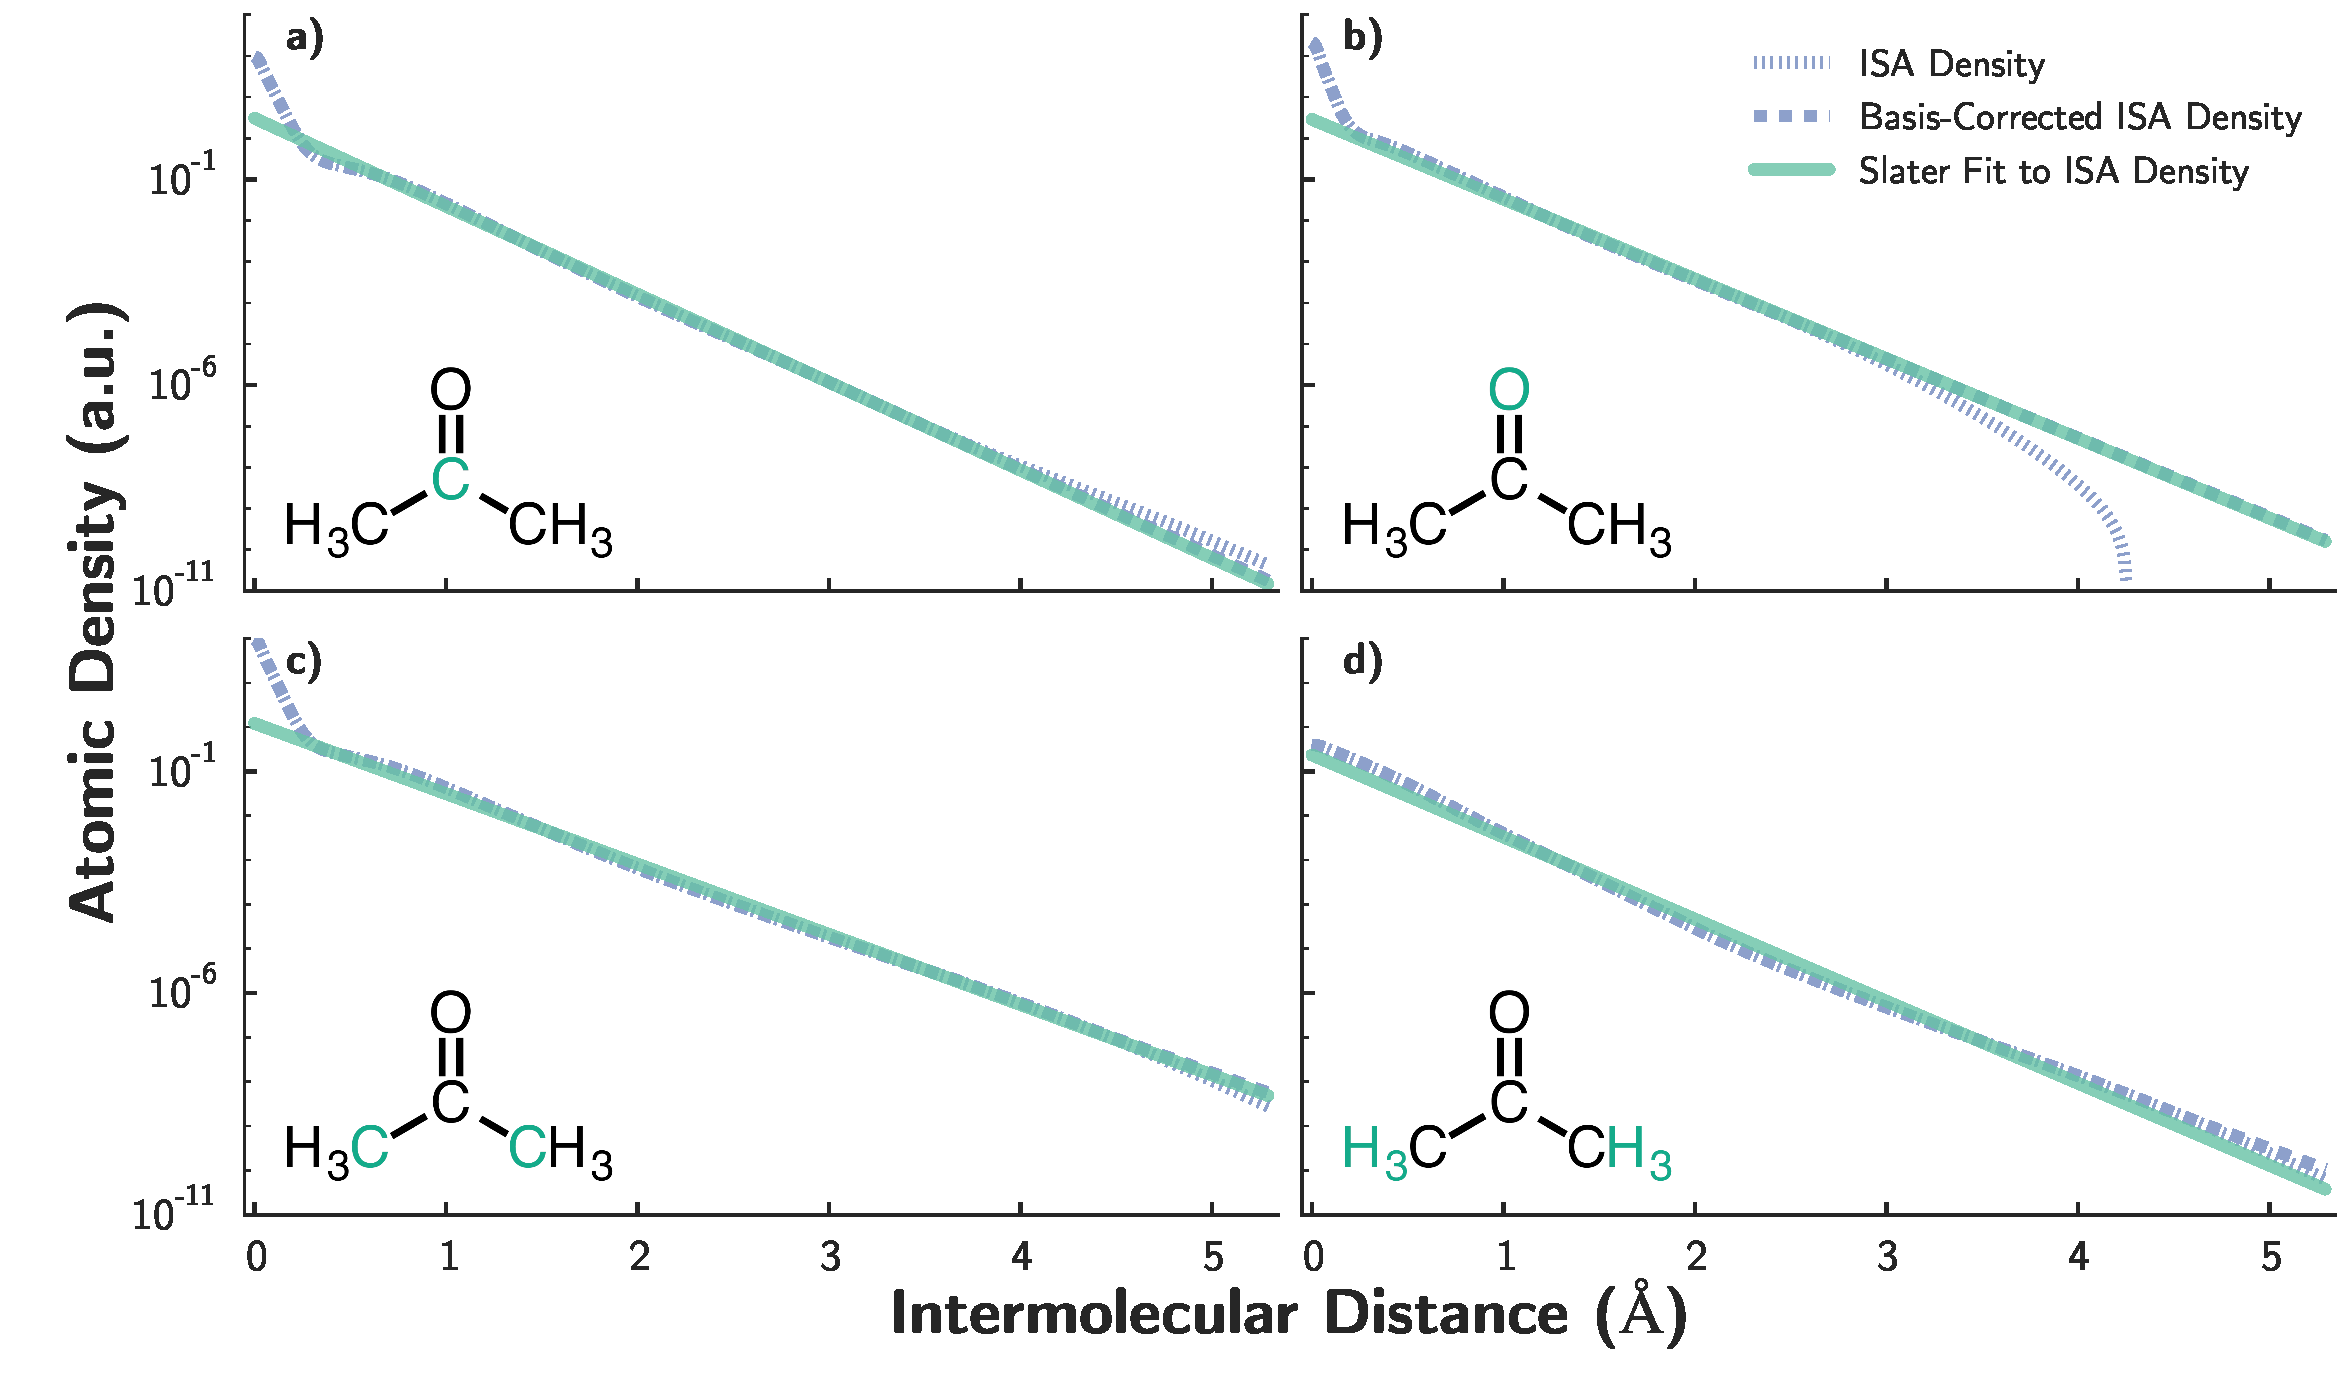
\includegraphics[width=0.9\textwidth]{isotropic/acetone_isa.pdf}  
    \caption{
        \bsisa and fitted shape functions for each atom type in acetone: a) carbonyl carbon,
        b) oxygen, c) methyl carbon, d) hydrogen. \bsisa shape functions (dotted line)
        for each atom type have been obtained at a
        PBE0/aug-cc-pVTZ level of theory. A modified \bsisa shape
        function (dashed line) corrects the tail-region of the \bsisa function to
        account for basis set deficiencies in the \bsisa algorithm. A single Slater
        orbital of the form $D_i^{\text{ISA}}\exp(-\Bisa{i} r)$ (solid line) is fit to the basis-corrected
        \bsisa shape function, and the obtained $\Bisa{i}$ value is used as an atomic exponent
        in the functional form of \isaff. Results for acetone are typical of
        molecules studied in this Chapter.
    		   }
    \label{fig:isotropic-bsisa}
    \end{figure}
    %%%%%%%%% Acetone-ISA %%%%%%%%%%%%%%%%%%%%

%ASK: Change 'basis-corrected' to 'tail-corrected?'
From \cref{fig:isotropic-bsisa} we see that the ISA atomic shape functions (that is, the
spherically-averaged ISA atoms-in-molecule density) 
decay exponentially outside the core region.
However, note that the exponents governing the spherical density decay, $\Bisa{i}$, 
differ from those of the free atoms. The ISA densities have been observed to account
for electron movement in the molecule, and the consequent density changes
brought about by this movement tend to be manifested in the region of the 
density tails. \cite{Misquitta2014}
The ISA exponents can be obtained by a weighted least-squares fit to the \bsisa atomic density
(see \cref{sec:isotropic-methods} for details), with the resulting fitted
atomic densities shown in \cref{fig:isotropic-bsisa}. 
Note that even a single exponential is remarkably successful in reproducing the
entirety of the valence atomic density.

Given these fitted ISA exponents, we can now apply
our short-range interaction formalism to polyatomics,
%
\begin{align}
\label{eq:isotropic-isaff_sr}
\begin{split}
V^{sr} &= \sum\limits_{ij} \Asr{ij} P(B_{ij}, r_{ij}) \exp(-B_{ij}r_{ij}) \\
P(B_{ij},r_{ij}) &= \frac13 (B_{ij} r_{ij})^2 + B_{ij} r_{ij} + 1 \\
    \Asr{ij} &= \Asr{i}\Asr{j} \\
    \B &= \sqrt{\Bisa{i}\Bisa{j}} \\
\end{split}
\end{align}
%
where the molecular
short-range energy is now a sum of atom-atom contributions. In conjunction
with appropriately damped atomic dispersion (\cref{eq:isotropic-ttdamp,eq:isotropic-isaff_ttdamp}), \cref{eq:isotropic-isaff_sr}  completely defines our new
short-range force field. We refer to this new functional form and set of atomic
exponents as the \isaff.

\end{subsection}


\end{section}
%%%%%%%%%%%%%%%%%%%%%%%%%%%%%%%%%%% Theory %%%%%%%%%%%%%%%%%%%%%%%%%%%%%%%%%%%%%%%%





%%%%%%%%%%%%%%%%%%%%%%%%%%%% Computational Details %%%%%%%%%%%%%%%%%%%%%%%%%%%%%%%%
\begin{section}{Computational Methods}
\label{sec:isotropic-methods}

%auto-ignore
To evaluate the \isaffold against conventional Born-Mayer and/or Lennard-Jones models, we compare the
ability of each resulting short-range force field to reproduce benchmark ab
initio intermolecular interaction energies for a collection of representative
dimers. Such a metric is directly relevant for ab initio force field
development. Even for an empirically-parameterized force field, however,
fidelity to an accurate ab initio potential should be well correlated with the
highest level of accuracy and transferability achievable with a given
short-range methodology. 

We have developed the \isaffold, Born-Mayer, and Lennard-Jones force fields using 
benchmark energies calculated using the symmetry-adapted perturbation theory
based on density-functional theory (DFT-SAPT or SAPT(DFT) 
\cite{Misquitta2002,Misquitta2003,Misquitta2005,Heßelmann2005a,Podeszwa2006a,Heßelmann2002,Heßelmann2003,Heßelmann2002a,Jansen2001}).
DFT-SAPT provides interaction energies that are comparable in accuracy to 
those from CCSD(T) and which are rigorously free from basis set superposition error.
\cite{Podeszwa2005a,Riley2010}
Additionally, at second-order, DFT-SAPT also provides an explicit interaction
energy decomposition into physically-meaningful contributions: 
the electrostatic, exchange-repulsion, induction, and dispersion energies.
This decomposition is vital to the development of models as it allows the
development of separate terms for each type of short-range interaction. 
Terms of third and higher order are estimated using the \dhf correction 
\cite{Jeziorska1987} which contains mainly higher-order induction contributions.
Following prior work,\cite{Yu2011,McDaniel2013} and for the purposes of
fitting to the DFT-SAPT data, we keep the second-order induction term and the
\dhf term separate.
%

Since the Slater-ISA and Born-Mayer force fields describe only short-range interactions (i.e. those terms which are modulated by
the overlap of the monomer electron densities), they must both be supplemented with additional long-range
terms that describe the electrostatic, polarization, and dispersion
interactions. Here we have chosen a long-range potential of the form 
%
\begin{align}
\label{eq:isotropic-elr}
\vlr &= V_{\text{multipole}} + V_{\text{dispersion}} + \vdrude \\
\intertext{where}
V_{\text{multipole}} &= \sum \limits_{ij} \vmultipole
\intertext{includes distributed multipole contributions from each atom up to
quadrupoles,} 
V_{\text{dispersion}} &= - \sum\limits_{ij}\sum\limits_{n=3}^{6} \frac{C_{ij,2n}}{r_{ij}^{2n}} 
\label{eq:isotropic-dispersion}
\end{align}
describes isotropic dispersion, and 
\vdrude is the polarization energy modeled by Drude oscillators 
\cite{drude1902theory, Lamoureux2003}
as in
\citen{McDaniel2013}.
%
The accuracy of each of these terms is expected to minimize errors in the
long-range potential, simplifying the comparison between short-range force field functional forms.
Nonetheless, we expect that our results will be qualitatively insensitive to
the particular choice of long-range force field and acknowledge that simpler alternatives may
be preferred for the development of highly efficient simulation potentials.
In the case of the Lennard-Jones force field, we replace \cref{eq:isotropic-dispersion} with
the simple $C_{ij,6}/r_{ij}^{6}$ dispersion term that is standard to the
Lennard-Jones model. 

We used a test set consisting of one atom (argon) and 
12 small organic molecules (see \cref{fig:isotropic-molecules}) from which dimer
potentials could be generated (we will use the term `dimer' to mean two,
potentially dissimilar, interacting molecules or atoms), 
yielding 91 dimer combinations (13 homo-monomeric, 78 hetero-monomeric).
This wide range of systems allowed us to evaluate both the accuracy and
transferability of the Slater-ISA model compared to conventional Born-Mayer
and/or Lennard-Jones models.

    %%%%%%%%% 91 Dimer Test Set %%%%%%%%%%%%%
    \begin{figure}
      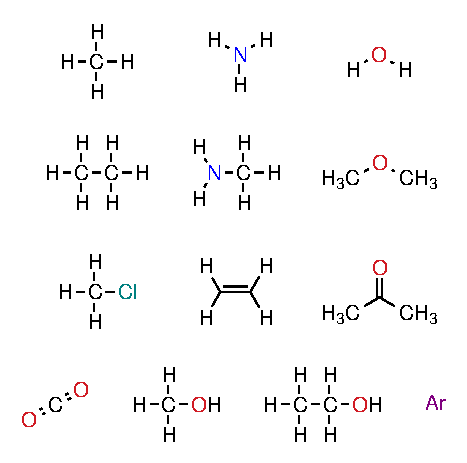
\includegraphics[width=0.6\textwidth]{isotropic/91_dimer_test_set.eps}
      \caption{
        The 13 small molecules included in the 91 dimer (13 homomonomeric, 78
        heteromonomeric) test set. Cartesian geometries for all of these
        molecules are given in \cref{sec:appendices-monomers}.
              }
      \label{fig:isotropic-molecules}
    \end{figure}
    %%%%%%%%% 91 Dimer Test Set %%%%%%%%%%%%%

A detailed description of this overall methodology is provided below.

\begin{subsection}{Construction of the 91 dimer test set}

Monomer geometries for each of the 13 small molecules were taken from the
experimental NIST
\mbox[CCCBDB] database\cite{Johnson2015NIST} and can be found in
\cref{sec:appendices-monomers}.
For acetone and methyl amine, experimental geometries were
unavailable, and thus
the computational NIST \mbox[CCCBDB] database was used to obtain geometries at
a high level of theory (B3LYP/\avtz for acetone, CCSD(T)/6-311G* for methyl
amine).
For each of the 91 dimers, a training set was constructed
using \saptpbeo interaction energies calculated at 1000 quasi-random dimer
configurations. These configurations were generated using Shoemake's
algorithm,\cite{Shoemake1992} subject to the constraint that the nearest atom pairs
be separated by between 0.75 and 1.3 of the sum of their van der Waals radii. 
This ensured adequate sampling of the potential 
energy surface in the region of the repulsive wall.
The DFT-SAPT interaction energies were evaluated using an asymptotically corrected
PBE0 functional (PBE0/AC) with monomer vertical (first) ionization potentials
computed using the $\Delta$-DFT approach at a PBE0/\avtz level of theory.
Unless otherwise noted, all DFT-SAPT calculations used an \avtz basis set in the 
dimer-centered form with midbond functions (the so-called DC+ form),
and were performed using the MOLPRO2009 software suite.\cite{MOLPRO-WIREs}
The midbond set consisted of a 5s3p1d1f even-tempered basis set with ratios
of 2.5 and centered at $\zeta = 0.5, 0.5, 0.3, 0.3$ for the s,p,d, and f shells,
respectively. This set was placed near the midpoint of the centers of mass of
the two interacting monomers.

A small fraction of DFT-SAPT calculations exhibited unphysical
energies, which were attributed to errors in generating the optimized
effective potential used during the \saptpbeo calculations; these points were
removed from the test set.

\end{subsection}
\begin{subsection}{\bsisa Calculations}


\bsisa atomic densities were obtained using CamCASP 5.8
\cite{camcasp5.8, WCMS:WCMS1172, orient4.8}
following the procedure of \citeauthor{Misquitta2014}\cite{Misquitta2014}
For the \bsisa calculations, an auxiliary basis was constructed from an RI-MP2
\avtz basis set with $s$-functions replaced by the ISA-set2
supplied with the CamCASP program;
CamCASP's ISA-set2 basis was also used for the ISA basis
set.\cite{Misquitta2014} A custom ISA basis set for Ar was used 
(even tempered, $n_{min} = -2, n_{max} = 8$)
\cite{Misquitta2014} 
as no published basis was available.
\bsisa calculations were performed with the A+DF algorithm, which allows the 
ISA functional to be mixed with some fraction, $\zeta$, of the density-fitting functional.
Following the recommendations of \citeauthor{Misquitta2014}\cite{Misquitta2014},
we have used $\zeta=0.1$ for the multipole moment calculations, 
and $\zeta=0.9$ for the density partitioning used to determine the \B coefficients. 


\end{subsection}
\begin{subsection}{Determination of $\Bisa{i}$}


The \bsisa-derived atomic exponents, $\Bisa{i}$, were obtained from a weighted
least-squares fit to the spherically averaged \bsisa atomic densities (shape functions),
$w_i(\mathbf{r})$.
In some cases, numerical instabilities and basis-set limitations of the \bsisa procedure
yielded densities that exhibited non-exponential asymptotic behavior.\cite{Misquitta2014}
To correct for these unphysical densities, we extrapolated the exponential decay
of the valence region to describe the \bsisa tails also. 
Details of this procedure can be found in
\cref{sec:workflow-exponent_algorithm}.
The ISA atom-in-molecule exponents were then derived via a log-weighted fit to
the tail-corrected shape-functions $w^a(\mathbf{r})$ for densities within the cutoff
$10^{-2} > w^a > 10^{-20}$ a.u.  This region was chosen to
reproduce the charge density most accurately in the valence regimes most likely to be relevant to
intermolecular interactions.


\end{subsection}
\begin{subsection}{Force Field Functional Forms and Parameterization}
    \label{sec:isotropic-FF-forms}

The general structure of the force fields \vtot for both the \isaffold and the 
Born-Mayer-type models are given by the following equations:

\begin{align}
%
\begin{split}
\label{eq:isotropic-bothff}
\vtot &= \sum\limits_{ij} \vrep_{ij} + \velst_{ij} + \vind_{ij} + \vdhf_{ij} +
\vdisp_{ij} \\[10pt]
\vrep_{ij} &= \Aex{ij} P(B_{ij}, r_{ij}) \exp(-B_{ij}r_{ij}) \\
\velst_{ij} &= -\Ael{ij} P(B_{ij}, r_{ij}) \exp(-B_{ij}r_{ij}) + \vmultipole \\
\vind_{ij} &= -\Aind{ij} P(B_{ij}, r_{ij}) \exp(-B_{ij}r_{ij}) + \vdrudeind \\
\vdhf_{ij} &= -\Adhf{ij} P(B_{ij}, r_{ij}) \exp(-B_{ij}r_{ij}) +
\vdrudescf \\
\vdisp_{ij} &= - \sum\limits_{n=3}^{6} f_{2n}(x) \frac{C_{ij,2n}}{r_{ij}^{2n}} \\
\A &= A_iA_j \\
\C &= \sqrt{C_{i,n}C_{j,n}} \\
f_{2n}(x) &= 1 - e^{-x} \sum \limits_{k=0}^{2n} \frac{(x)^k}{k!} \\
\end{split}
%
\intertext{For the \isaffold:}
%
\begin{split}
\label{eq:isotropic-isaff}
B_i &= \Bisa{i} \\
\B &= \sqrt{B_iB_j} \\
P(B_{ij},r_{ij}) &= \frac13 (B_{ij} r_{ij})^2 + B_{ij} r_{ij} + 1 \\
x &= B_{ij}r_{ij} - \frac{2 B_{ij}^2 r_{ij} + 3 B_{ij} }
{ B_{ij}^2 r_{ij}^2 + 3 B_{ij} r_{ij} + 3} r_{ij}
\end{split}
%
\intertext{For all Born-Mayer type models:}
%
\begin{split}
P(B_{ij},r_{ij}) &= 1 \\
x &= B_{ij}r_{ij}
\end{split}
%
\intertext{For the \saptff:}
%
\begin{split}
\label{eq:isotropic-saptff}
B_i &\equiv \Bip{i} = 2\sqrt{2I_i} \\
\B &= \frac{B_iB_j(B_i + B_j)}{B_i^2 + B_j^2}
\end{split}
%
\intertext{For the \bmsisaff:}
%
\begin{split}
    B_i &= 0.84\Bisa{i} \\
    \B &= \sqrt{B_iB_j}
\end{split}
%
\end{align}
%

Of the parameters in these force fields, only the coefficients $A_i$ were fit
to reproduce DFT-SAPT dimer energies (details below). All other force field
parameters were derived from first-principles atom or atom-in-molecule properties.
Exponents for the \isaffold and the \bmsisaff were derived from \bsisa calculations,
while exponents for the \saptff were determined from vertical ionization potentials
of the isolated atoms.
Dispersion coefficients (\C) were either used directly from \citen{McDaniel2013} or
were parameterized using analogous methods in the case of argon.
Distributed multipoles $Q_t^i$ for each system were obtained from the \bsisa-based
distributed multipoles scheme (ISA-DMA) \cite{Misquitta2014}, with the expansion
truncated to rank 2 (quadrupole). 
Note that here, $t=00,10,\dots,22s$ denotes the rank of the multipole in 
the compact notation of \citeboth{stone2013theory}.
% AJM : This is a bit confusing. Can you explain?
(In addition to rank 2 ISA-DMA multipoles, we also tested the use of DMA4
multipoles\cite{Stone2005} 
as well as the use of rank 0 charges obtained from the 
rank truncation or transformation\cite{Ferenczy1997} of either ISA-DMA or DMA4
multipoles; the effect of including a Tang-Toennies damping
factor\cite{McDaniel2013,Tang1984} was studied in all cases.
Each of these alternative long-range electrostatic models proved either
comparably or less accurate for both the \isaffold and the \saptff in terms of their
ability to reproduce the DFT-SAPT electrostatic energy, and are not discussed
further.)
Long-range polarization ($V_{shell}$) was modeled using Drude oscillators in a manner
identical to \citen{McDaniel2013}. As in our prior work, during parameterization,
the Drude energy was partitioned into 2\super{nd} (\vdrudeind) and 
higher order (\vdrudescf) contributions, where \vdrudeind is the Drude oscillator
energy due to static charges (excluding intra-molecular contributions), and
\vdrudescf is the difference between the fully converged Drude energy,
$V_{shell}$, and \vdrudeind.  Force field parameters for all homo-monomeric
systems are located in the \si of \citen{VanVleet2016}. 

A weighted least-squares fitting procedure was used to fit $A_i$
parameters to the benchmark \saptpbeo interaction energies on a 
component-by-component basis.
That is, four separate optimizations\cite{McDaniel2013}  were
performed to directly fit \vrep, \velst, \vind, and \vdhf to, respectively, the
following DFT-SAPT quantities (notation as in \citen{Heßelmann2005a}):
%
\begin{align}
\begin{split}
\erep &\equiv E^{(1)}_{\text{exch}} \\
\eelst &\equiv E^{(1)}_{\text{pol}} \\
\eind &\equiv E^{(2)}_{\text{ind}} + E^{(2)}_{\text{ind-exch}} \\
\edhf &\equiv \delta(\text{HF}).
\end{split}
%
\intertext{
For \vdisp, no parameters were directly fit to the DFT-SAPT dispersion,
}
%
\edisp &\equiv E^{(2)}_{\text{disp}} + E^{(2)}_{\text{disp-exch}},
\end{align}
%
but were instead obtained solely from monomer properties as described above.
Finally, note that no parameters were directly fit to the total DFT-SAPT
energy,
%
\begin{align}
\etot = \erep + \eelst + \eind + \edhf + \edisp,
\end{align}
%
for either the \isaffold or the \saptff. Rather, \vtot was calculated according to \cref{eq:isotropic-bothff}.

Data points for each fit were weighted using a Fermi-Dirac functional form
given by
%
\begin{align}
\label{eq:isotropic-weighting-function}
w_i = \frac{1}{\exp((-E_i - \mu_{\text{eff}})/kT) + 1},
\end{align}
%
where $E_i$ is the reference energy and $\mu_{\text{eff}}$ and $kT$ were treated as
adjustable parameters. The parameter $kT$, which sets the energy scale for the
weighting function, was taken to be $kT = \lambda |E_{\text{min}}|$; here $E_{\text{min}}$
is an estimate of the global minimum well depth. Unless otherwise stated, we have used
$\lambda = 2.0$ and $\mu_{\text{eff}} = 0.0$.   
These defaults were chosen to minimize overall average attractive RMSE for all 91 dimer
sets. 
Increases or decreases in the $\lambda$ factor correspond to the weighting of
more or fewer repulsive configurations, respectively.  

In the case of Lennard-Jones, the standard Lennard-Jones functional form was
used for the van der Waals terms, with Coulomb and polarization terms modeled
exactly as for the \isaffold:
\begin{align}
%
\vtot^{\text{LJ}} &= \sum\limits_{ij} \frac{A_{ij}}{r^{12}_{ij}} - \frac{C_{ij,6}}{r^{6}_{ij}} + \vdrude + \vmultipole
%
\end{align}
%
Lorentz-Berthelot combination rules were used to obtain heteroatomic $A_{ij}$
and $C_{ij}$ parameters. Unlike with the \isaffold and Born-Mayer models, $\vtot^{\text{LJ}}$ was fit to
the total \saptpbeo energy, with $A_{ij}$ and $C_{ij,6}$ as fitting parameters. The
weighting function from \cref{eq:isotropic-weighting-function} was used in fitting.

%% In order to also compare the \isaffold to simple non-polarizable Lennard-Jones force
%% fields, we also parameterized a version of $\vtot^{\text{LJ}}$ using only rank 0 charges and
%% $\vdrude = 0$; these results are shown in the Supporting Information.

\end{subsection}
\begin{subsection}{Potential Energy Surface Scans}


In order to visually assess fit quality, representative one-dimensional scans
of the potential energy surface were calculated for several dimer pairs along
low-energy dimer orientations. For each dimer pair, the minimum energy
configuration of the 1000 random dimer points was selected as a starting
configuration, and additional dimer configurations (not necessarily included in the
original 1000 points) were generated by scanning along some bond vector. In the case of the
ethane dimer, two carbon atoms (one on each monomer) were used; for acetone,
the carbonyl carbon on each monomer defined the bond vector.


\end{subsection}


\begin{subsection}{Molecular Simulations}

All bulk simulations were run using OpenMM release version 7.0.
\cite{Eastman2013}
Enthalpies of vaporization were computed from 
%
\begin{align*}
\Delta H_{\text{vap}} = (E_{\text{pot}}(g) + RT) - E_{\text{pot}}(l)
\end{align*}
%
where $E_{\text{pot}}(g)$ and $E_{\text{pot}}(l)$ were determined from NVT
simulations at the experimental gas and liquid densities, respectively.
Calculated liquid
densities were determined from NPT simulations. In all cases, the OPLS/AA
force field was used for the intramolecular potential.
\cite{Jorgensen1996}
All simulations used a Langevin integrator with a 0.5 fs time step and a 1
ps$^{-1}$ friction coefficient; NPT simulations used a Monte Carlo barostat
with a trial volume step every 5\super{th} move. Periodic boundary conditions,
particle-mesh Ewald, and a non-bonding cutoff of 1.2nm with added long-range
corrections were used to simulate a
unit cell of 222 molecules. After an equilibration period
of at least 600ps, simulation data was gathered from production runs lasting
at least 200ns. 



\end{subsection}


\end{section}
%%%%%%%%%%%%%%%%%%%%%%%%%%%% Computational Details %%%%%%%%%%%%%%%%%%%%%%%%%%%%%%%%




%%%%%%%%%%%%%%%%%%%%%%%%%%%%%%%%%% Results %%%%%%%%%%%%%%%%%%%%%%%%%%%%%%%%%%%%%%%%
\begin{section}{Results and Discussion}
\label{sec:isotropic-results}

%% \begin{subsection}{Overview}

The Slater-ISA methodology for short-range intermolecular interactions has
been derived from a simple but rigorous physical model of overlapping
monomer electron densities. In practice, this approach differs from the
conventional Born-Mayer approach in both the choice of the short-range
functional form (with the latter omitting the polynomial pre-factor) and the
source of the exponents (with the former derived from ISA analysis of the
monomer density). Our principal goal is to examine the influence of these
modifications on the accuracy and transferability of the resulting force
fields.

We initially benchmark the \isaffold against a conventional Born-Mayer potential,
\saptff.
%, where the -IP suffix denotes the fact that the atomic exponents $B_i$ have
%been derived from the isolated atomic ionization potentials.  
The latter approach has been used extensively in prior
work,\cite{Schmidt2015,McDaniel2013} and both approaches use identical numbers of
fitted parameters.  Following prior work, combination rules for the \saptff are as in
\citen{McDaniel2013}. (We have tested the effect of using a geometric mean
for the \saptff; results do not differ qualitatively from those presented
below.) Owing to its popularity, we also compare the \isaffold to a Lennard-Jones
functional form (\ljff).

We first assess the accuracy of the \isaffold, \saptff, and \ljff against benchmark
ab initio intermolecular interaction energies and experimental 2\super{nd}
virial coefficients, enthalpies of vaporization, and liquid densities. 
We next examine parameter transferability, assessing the
extent to which parameters from pure homo-monomeric systems can be re-used
(without further optimization) to describe mixed interactions. To assess 
parameter robustness, we also study the sensitivity of each methodology to
changes in the weighting function (\cref{eq:isotropic-weighting-function}). Finally, we
explore the application of \bsisa-derived exponents within the Born-Mayer
functional form as a straightforward method for simplifying the
parameterization (and potentially increasing the accuracy) of a wide variety of
standard ab initio and empirically-parameterized force fields.


\begin{subsection}{Accuracy: Comparison with DFT-SAPT}

For each of the 91 molecule pairs described in the \nameref{sec:isotropic-methods} section, 
parameters for the \isaffold, \saptff, and \ljff
were fit to reproduce \saptpbeo interaction energies calculated for a set of 1000 dimer
configurations. These 91,000 total configurations and corresponding DFT-SAPT
energies are collectively referred to as the `91 dimer test set'.  As a
primary indication of accuracy, root-mean-square errors (RMSE) and mean signed
errors (MSE), both with respect to DFT-SAPT, were computed for each
methodology and for each dimer pair. Because these RMSE and MSE are dominated by
repulsive contributions, and owing to the thermodynamic importance of
attractive configurations, so-called `attractive RMSE/MSE' were also computed by
excluding net repulsive configurations (as measured by the DFT-SAPT total energy). 
The overall RMSE/MSE for all 91 dimers were then
averaged to produce one `characteristic RMSE/MSE' for the entire test set.  Since
these errors varied considerably in magnitude depending on the dimer in
question, this overall average was taken in the geometric mean sense. (Results
with an arithmetic mean do not differ qualitatively). Note that when computing
the characteristic MSE, only the magnitude of each MSE, \mse, was considered.

Characteristic RMSE and \mse across the 91 dimer test set are shown in \cref{fig:isotropic-rmse}
and \cref{tab:isotropic-rmse}.  Overall, the \isaffold exhibits smaller errors compared
to the \saptff. On average, the characteristic total energy RMSE for the \isaffold
decrease by 33\% relative to the \saptff.  Even excluding repulsive configurations
(dominated by short-range interactions), errors for the \isaffold are lower by 11\%
compared to the \saptff, demonstrating modest gains in accuracy even over the most
energetically-relevant regions of the potential.  
A more detailed analysis of each of the 91 pairs of molecules shows that in an
overwhelming 93\% of such cases, force fields
derived from the Slater-ISA method have smaller RMSEs compared to their
Born-Mayer-IP counterparts (70\% if only attractive configurations are
considered). Regardless of the metric used, the \isaffold produces force
fields with higher fidelity to the underlying benchmark interaction energies.

    %%%%%%%%%%%% Average RMSE %%%%%%%%%%%%%%%
    \begin{figure}
    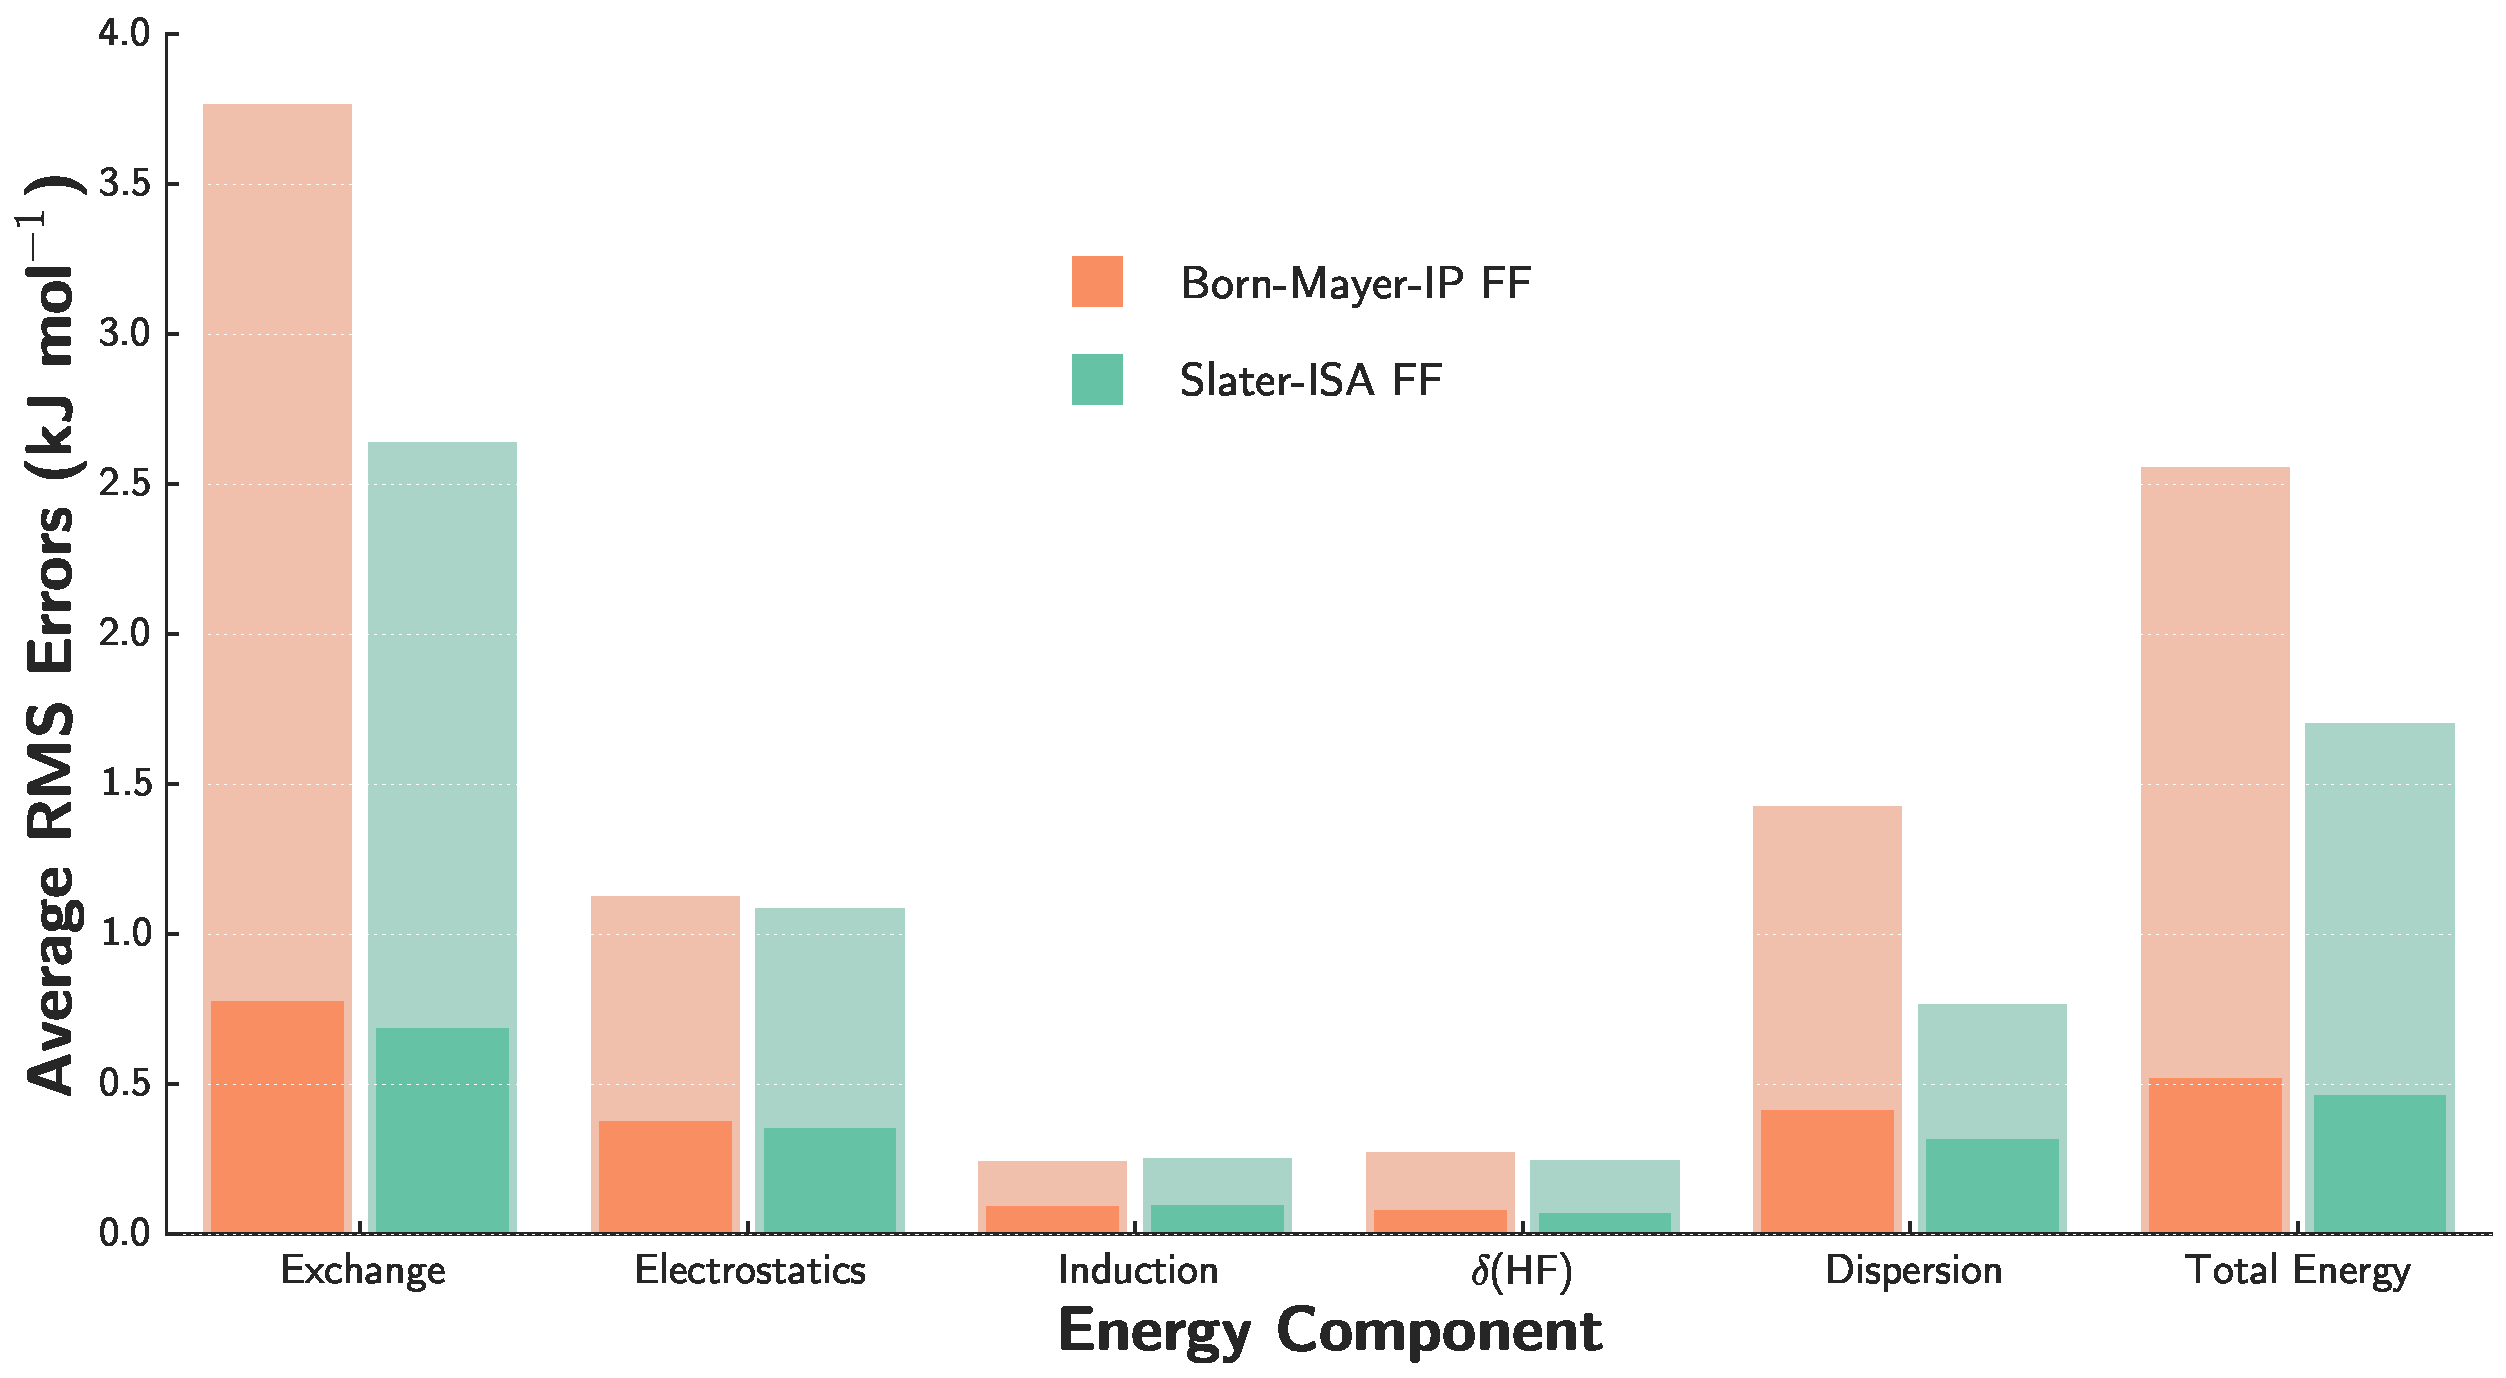
\includegraphics[width=0.9\textwidth]{isotropic/rmse_errors.pdf}
    \caption{
    Characteristic RMSE (as described in the main text) for the \saptff (orange) and the \isaffold (green) over the 91
    dimer test set. The translucent bars represent total RMSE
    for each energy component, while the smaller solid bars represent `Attractive'
    RMSE, in which repulsive points have been excluded.
            }
    \label{fig:isotropic-rmse}
    \end{figure}
    %%%%%%%%%%%% Average RMSE %%%%%%%%%%%%%%%

%%%%%%%%%%%%%%%%%%%%% Average RMSE Table %%%%%%%%%%%%%%%%%%%%%%%%%%%%%%%%%%%
\begin{landscape}
\begin{table}
\footnotesize
\centering
\renewcommand\arraystretch{1.1}
\begin{tabular}{@{}rcccccccc@{}}
\hline
\toprule
& \phantom{} &
  \multicolumn{3}{c}{Dimer-Specific Fits} &
  \phantom{ab} &
  \multicolumn{3}{c}{Transferable Fits} \\
\cmidrule{3-5} \cmidrule{7-9}

Component & & \isaffold & \saptff & \ljff & & \isaffold & \saptff & \ljff \\
     & & \multicolumn{1}{c}{(kJ mol$^{-1}$)} & \multicolumn{1}{c}{(kJ mol$^{-1}$)} &  \multicolumn{1}{c}{(kJ mol$^{-1}$)}
     & & \multicolumn{1}{c}{(kJ mol$^{-1}$)}& \multicolumn{1}{c}{(kJ mol$^{-1}$)} &  \multicolumn{1}{c}{(kJ mol$^{-1}$)}\\
\midrule
Exchange        & &    2.641 (0.686)   &    3.766 (0.775)   &     ---          & &    2.718 (0.720)  &    4.033 (0.836)   &     ---        \\
Electrostatics  & &    1.087 (0.351)   &    1.126 (0.377)   &     ---          & &    1.134 (0.351)  &    1.231 (0.378)   &     ---        \\
Induction       & &    0.251 (0.095)   &    0.241 (0.093)   &     ---          & &    0.278 (0.101)  &    0.265 (0.098)   &     ---        \\
\dhf            & &    0.246 (0.068)   &    0.272 (0.079)   &     ---          & &    0.274 (0.076)  &    0.304 (0.081)   &     ---        \\
Dispersion      & &    0.766 (0.317)   &    1.425 (0.414)   &     ---          & &    0.766 (0.317)  &    1.425 (0.414)   &     ---        \\
\addlinespace
\textbf{
Total Energy}  \\
\emph{RMSE}     & &    1.701 (0.464)   &    2.554 (0.520)   &   1.984 (0.603)  & &    1.650 (0.456)  &    2.698 (0.555)   &  2.054 (0.640) \\
%\addlinespace
%Average Absolute MSE    
\emph{\mse}
                & &    0.216 (0.057)   &    0.539 (0.127)   &    0.322 (0.345) & &    0.175 (0.051)  &    0.569 (0.112)  &    0.311 (0.368) \\
\bottomrule
\hline
\end{tabular}
\caption{
    Comparison of characteristic RMSE (as described in the main text) over the 91 dimer test
set for the \isaffold, \saptff and \ljff.
For the total energy, both characteristic RMSE and MSE have been shown, with
only the magnitude of the MSE, \mse, displayed.
    `Attractive' RMSE, representing the characteristic RMSE for
    the subset of points whose energies are net attractive ($\etot <
    0$), are shown in parentheses to the right of the total RMS
    errors; `attractive' \mse are likewise displayed for the total
    energy.
As discussed in \cref{ss:transferability}, the `Dimer-Specific Fits'
refer to force fields whose parameters have been optimized for each of the 91
dimers separately, whereas the `Transferable Fits' refer
to force fields whose parameters have been optimized for the 13 homodimers and
then applied (without further optimization) to the remaining 78 mixed systems.
    Unless otherwise stated, a default weighting function of $\lambda=2.0$
    (see \cref{eq:isotropic-weighting-function}) has been used for all force fields in
    this Chapter.
	}
\label{tab:isotropic-rmse}
\end{table}
\normalsize
\end{landscape}
%%%%%%%%%%%%%%%%%%%%% Average RMSE Table %%%%%%%%%%%%%%%%%%%%%%%%%%%%%%%%%%%

It is also instructive to consider each energy component individually.  As
might be expected, improvements in the description of \erep are pronounced,
with the characteristic RMSE from the \isaffold being 30\% smaller than that from the \saptff.
Examining each dimer pair separately (see
\cref{sec:isotropic-homomonomeric_fits} for homo-monomeric
fits, representative of the entire test set) we also find that, in general, the \isaffold
is far better at reproducing \emph{trends} in the exchange energy compared to
the \saptff. This qualitative result is also reflected in the smaller \mse
values for the \isaffold as compared to the \saptff.
Nevertheless, there remains a fair amount of scatter in the exchange
energies for several dimer pairs, particularly for molecules with exposed lone
pairs or delocalized $\pi$ systems. We hypothesize that this scatter is due to
a breakdown of the isotropic approximation made in the \nameref{sec:isotropic-theory}
section, a conclusion supported by observations on the pyridine dimer system
recently made by some of us.\cite{Misquitta2015b}
It it therefore quite possible that the observed 30\% RMSE reduction 
underestimates the true error reduction that might be observed
if such anisotropy were accounted for.

From  \cref{fig:isotropic-rmse}, we see that the dispersion energy model from the 
\isaffold is also a substantial improvement; for dispersion, characteristic RMSE
are 46\% smaller for the \isaffold compared to the Born-Mayer model.
This should not be a counter-intuitive result: while both potentials use identical
dispersion coefficients, they differ in the damping model used.
In the \saptff, the standard Tang--Toennies damping model is employed, and 
the damping parameters only depend on free atom ionization potentials; 
in the \isaffold, on the other hand, the damping parameters are obtained from the
ISA shape functions, and thus take 
molecular environment effects into account.
Even when only considering attractive dimer configurations (solid bar in
\cref{fig:isotropic-rmse}), errors in the dispersion energy component are reduced by 23\%,
demonstrating the importance of the damping function across the potential surface. 
From these results, and in agreement with related literature
studies,\cite{Sebetci2010} we conclude that use of
the standard Tang-Toennies damping function based on atomic ionization
potentials
\cite{Tang1984, Misquitta2008a, Price2010, Totton2010a, McDaniel2013, Hermida-Ramon2000, Nyeland1990} 
lacks quantitative predictive power compared to the Slater-ISA model.
Note that neither the \isaffold nor the \saptff are directly fitted to the DFT-SAPT
dispersion energies (all parameters are determined from monomer properties),
making this accuracy particularly striking.  We hypothesize that the effect of
the Slater-ISA approach is greater for dispersion than for first-order exchange
because here (in contrast to the exchange energy) there are no fitted
parameters to compensate for deficiencies in the exponents or functional form
of the \saptff.

In contrast to the exchange and dispersion energies, the \isaffold and the \saptff show nearly identical errors for the
electrostatic and the induction (2\super{nd} order induction plus \dhf) energies.
In these cases, the two models differ only in the parameters and functional form used to represent
the exponentially-dependent short-range terms of these energy components, 
namely the penetration component for the electrostatic term and the 
penetration/charge-transfer term for the induction.
The lack of improvement between the Slater-ISA and Born-Mayer-IP models may
imply that we are not 
able to capture the physics of these particular short-range interactions with
either the Slater-functional of Born-Mayer functional forms.
Alternatively, the assumption that the short-range components of the electrostatic 
and induction energies are proportional to the exchange-repulsion may need to be 
re-examined. As discussed in \cref{sec:isotropic-heteroatomic_vsr},
this proportionality is known to be approximately valid, but as yet there does 
not seem to be a deeper theoretical understanding of these short-range terms
that may lead to a better model.
Nevertheless, absolute errors in the electrostatic and induction components are
relatively small for both models.  Thus overall, the \isaffold functional form
is promising for treating a wide variety of short-range effects. 


%%%%%%%%%%%%%%%%%%%%% Average LJ RMSE Table %%%%%%%%%%%%%%%%%%%%%%%%%%%%%%%%%%%
%\begin{landscape}
\begin{table}
\footnotesize
\centering
\renewcommand\arraystretch{1.1}
\begin{tabular}{@{}rcccccc@{}}
\hline
\toprule
& \phantom{} &
  \multicolumn{2}{c}{\ljff Dimer-Specific Fits} &
  \phantom{ab} &
  \multicolumn{2}{c}{\ljff Transferable Fits} \\
\cmidrule{3-4} \cmidrule{6-7}

%% Component & & \ljff-q0, $\lambda=0.1$ & \ljff-q2, $\lambda=0.1$ & \ljff-q2, $\lambda=2.0$ 
%%           & & \ljff-q0, $\lambda=0.1$ & \ljff-q2, $\lambda=0.1$ & \ljff-q2, $\lambda=2.0$ \\

%%           & & \ljff               & \ljff             %  & \ljff-q0,               
%%           & & \ljff               & \ljff       \\    %  & \ljff-q0,               \\
          & &           $\lambda=2.0$ &           $\lambda=0.1$      %     $\lambda=0.1$ 
          & &           $\lambda=2.0$ &           $\lambda=0.1$   \\ %     $\lambda=0.1$ \\
     & & \multicolumn{1}{c}{(kJ mol$^{-1}$)} & \multicolumn{1}{c}{(kJ mol$^{-1}$)} % &  \multicolumn{1}{c}{(kJ mol$^{-1}$)}
     & & \multicolumn{1}{c}{(kJ mol$^{-1}$)}& \multicolumn{1}{c}{(kJ mol$^{-1}$)}  \\ % &&  \multicolumn{1}{c}{(kJ mol$^{-1}$)}\\
\midrule
%% RMSE             & &  1.984 (0.603)   &  6.058 (0.413)  &  5.116 (0.560)   && 2.054 (0.640)  &  5.760 (0.457)  &  4.513 (0.658) \\
%% Absolute MSE
%%                  & &  0.322 (0.345)   &  1.610 (0.041)  &  0.803 (0.038)   && 0.311 (0.368)  &  1.410 (0.060)  &  0.562 (0.079) \\
\emph{RMSE}             & &  1.984 (0.603)   &  6.058 (0.413)  && 2.054 (0.640)  &  5.760 (0.457)    \\
\emph{\mse}
                 & &  0.322 (0.345)   &  1.610 (0.041)  && 0.311 (0.368)  &  1.410 (0.060)    \\
\bottomrule
\hline
\end{tabular}
\caption{
    Comparison of characteristic RMSE and \mse over the 91 dimer test
set for the various Lennard-Jones models. The LJ models are not parameterized
on a component-by-component basis, thus RMSE/\mse values are only
shown for the total FF energies.
    `Attractive' errors, representing the characteristic RMSE/\mse for
    the subset of points whose energies are net attractive ($\etot <
    0$), are shown in parentheses to the right of the total 
    errors. `Dimer-Specific Fits' and `Transferable Fits' are as in \cref{tab:isotropic-rmse}.
	}
\label{tab:isotropic-lj_rmse}
\end{table}
\normalsize
%\end{landscape}
%%%%%%%%%%%%%%%%%%%%% Average LJ RMSE Table %%%%%%%%%%%%%%%%%%%%%%%%%%%%%%%%%%%


The comparison between the \isaffold and the \ljff is slightly more complicated,
owing to the differences in long-range potential and fitting methodology (see
\cref{sec:isotropic-FF-forms}). As such, we compare the \isaffold to several versions of the
\ljff (for which characteristic RMSE and \mse are shown in 
\cref{tab:isotropic-lj_rmse}). Using the same weighting function and
constraining the Coulombic and polarization terms to be identical to the
\isaffold, we see that the resulting Lennard-Jones force field (\ljff,
$\lambda=2.0$) is significantly worse than the \isaffold, both in terms of total
RMSE and attractive RMSE. Furthermore, by comparing the \mse
of both force fields, we see that errors in
\ljff are much more \emph{systematic} than in the \isaffold: in order to
reproduce the repulsive wall correctly, the Lennard-Jones potential
generally underestimates the well-depth by a considerable fraction (see
the Supporting Information of \citen{VanVleet2016} for ethane as a typical example). 

Given the failure of the \ljff ($\lambda=2.0$) force field to reproduce the
energetically important region of the PES, we also compared the \isaffold to a
`best-case' scenario Lennard-Jones force field which correctly
reproduces the minimum energy region at the expense of the repulsive wall. These
\ljff ($\lambda=0.1$) fits have total RMSE errors nearly 4 times that of the
\isaffold; indeed, the \ljff ($\lambda=0.1$) reproduces the repulsive wall only
qualitatively. Insofar as the repulsive wall is concerned, the \isaffold is far
superior to the Lennard-Jones short-range model. Nevertheless (and much more
importantly for molecular simulation), the attractive region of the potential
is reproduced surprisingly well by \ljff. Characteristic attractive RMSE for
the \ljff ($\lambda=0.1$) are slightly lower than those for \isaffold, although
the former has one additional free parameter per atom type and is also fit directly
to reproduce the total energy. Likewise, attractive \mse between the
\isaffold and the \ljff ($\lambda=0.1$) are comparable. As we show in the
Supporting Information of \citen{VanVleet2016},
however, and as is well known in the literature, weighting the Lennard-Jones potential in this
manner does not necessarily capture important information from the long-range attractive tail or repulsive wall of the PES, such
that the \ljff ($\lambda=0.1$) is not always expected to yield good
property predictions. This latter point will be demonstrated in 
\cref{sec:isotropic-accuracy_experiment}.

In order to compare the performance of the \isaffold against popular standard
force fields, we also developed a `best case scenario' non-polarizable point
charge Lennard-Jones model, results for which are shown in the Supporting
Information of \citen{VanVleet2016}. Unsurprisingly, this force field is worse (in an
RMSE and \mse sense) than all
other force fields studied in this Chapter, thus demonstrating how important
accurate models for long-range electrostatics and polarization are to the
overall accuracy of ab initio force fields.

\begin{subsubsection}{Argon Dimer}

We now turn to several specific case studies. The Ar dimer provides an interesting test
case to examine directly the impact of the polynomial pre-factor included in
the \isaffold functional form. 
Since Ar is an atomic species, we should have $\Bisa{\text{Ar}} = \Bip{\text{Ar}}$.
For numerical reasons, the \isaffold and \saptff exponents differ by 0.03 a.u.;
however, this difference is insignificant, and the two FFs differ mainly in the
polynomial pre-factor.
\cref{fig:isotropic-ar-pes} shows the potential energy
surface (PES) for the argon dimer computed using the \isaffold and the \saptff.
Here the default weighting scheme has been used so as to best reproduce the energetically
attractive region. Note that, while both potentials reproduce the minimum energy
configurations correctly, the \saptff considerably overestimates the exchange energy (and thus
the total energy) along the repulsive wall.
The \isaffold, on the other hand, maintains excellent accuracy in this region of the
potential. This result is particularly notable because the repulsive wall is not heavily weighted in the fit.
(A point 10 kJ mol$^{-1}$ along the repulsive wall, for instance, is weighted only 3\% as
heavily as a point near the bottom of the well).
A similar, though smaller, increase in accuracy is seen in the fit to the
DFT-SAPT dispersion energies, where the \isaffold is better able to model the
energies for shorter interatomic separations.  This increased accuracy is
entirely attributable to the functional form employed, as the dispersion
parameters are identical between the two FFs.

Consistent with prior literature,\cite{Ihm1990, McDaniel2012} these results
suggest that neglect of the polynomial pre-factor $P$ (as in standard
Born-Mayer potentials) is \emph{by itself} a poor approximation. However, as
we show below, the Born-Mayer form can still be used as an accurate model
in conjunction with appropriately scaled atomic exponents. Nonetheless, the
more physically-motivated Slater form provides increased accuracy over a wider
range of separations without recourse to empirical scaling.


    %%%%%%%%%%%% Ar-Ar PES %%%%%%%%%%%%%%%%%%
    \begin{figure}
    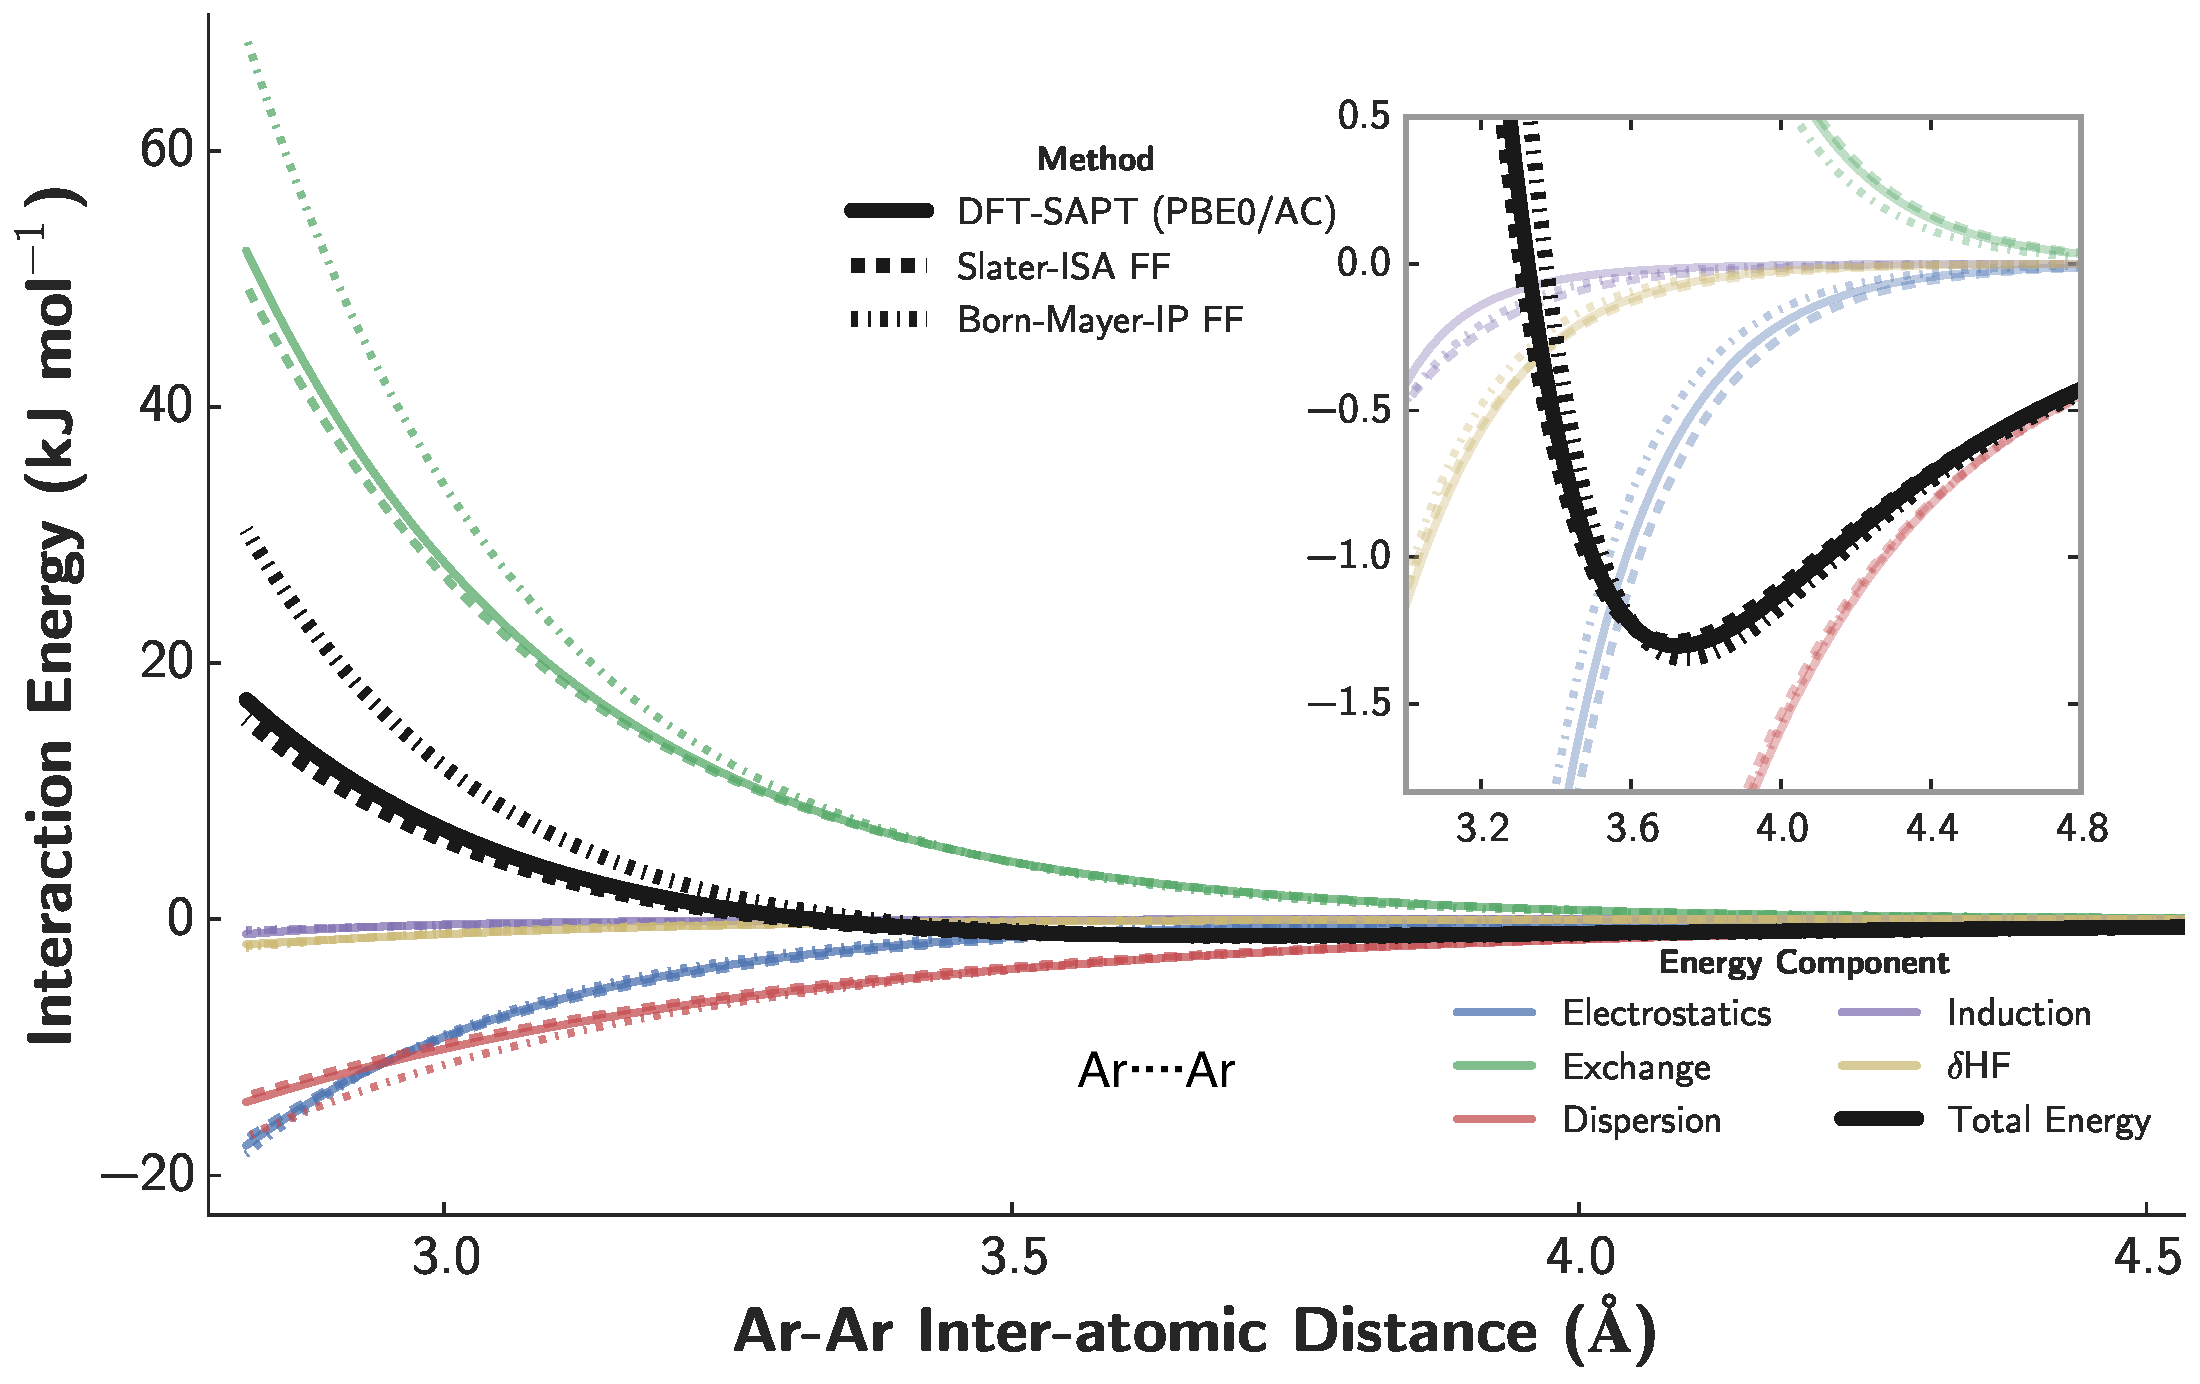
\includegraphics[width=0.9\textwidth]{isotropic/ar_ar_pes.pdf}
    \caption{
    Potential energy surface for the argon dimer. 
    Interaction energies for the \isaffold (dashed curves) and the \saptff (dash-dotted
    curves) are shown alongside benchmark \saptpbeo energies (solid curves). The
    energy decomposition for DFT-SAPT and for each force field is shown for reference.
    }
    \label{fig:isotropic-ar-pes}
    \end{figure}
    %%%%%%%%%%%% Ar-Ar PES %%%%%%%%%%%%%%%%%%

Results for \ljff are shown in the Supporting Information of
\citen{VanVleet2016}; consistent with expectations for the
Lennard-Jones model, the repulsive wall is overestimated by the
$1/r_{ij}^{12}$ short-range functional form, and the magnitude of the
attractive tail region is similarly overestimated by the effective $C_{ij,6}$
dispersion parameter. 
%
Note that this $C_{ij,6}$ coefficient has been fit to the total energy, and thus differs
from the asymptotically-correct $C_{ij,6}$ parameter used for both the \isaffold
and the \saptff. 
An alternative parameterization strategy would have been to use the asymptotically-correct $C_{ij,6}$
parameter in the \ljff, but this would have worsened predictions
along both the repulsive wall and the
minimum energy configurations.


\end{subsubsection}
\begin{subsubsection}{Ethane Dimer}


We next discuss the ethane dimer and show both a scatter plot
of the 1000 dimer interactions (\cref{fig:isotropic-ethane-scatter}) and a cut through the
potential energy surface near the minimum (\cref{fig:isotropic-ethane-pes}) as
indications of force field quality.

    %%%%%%%% Ethane-Ethane Scatter %%%%%%%%%%
    \begin{figure}
    %\includegraphics[width=0.9\textwidth]{ammonia_ff_quality.png}
    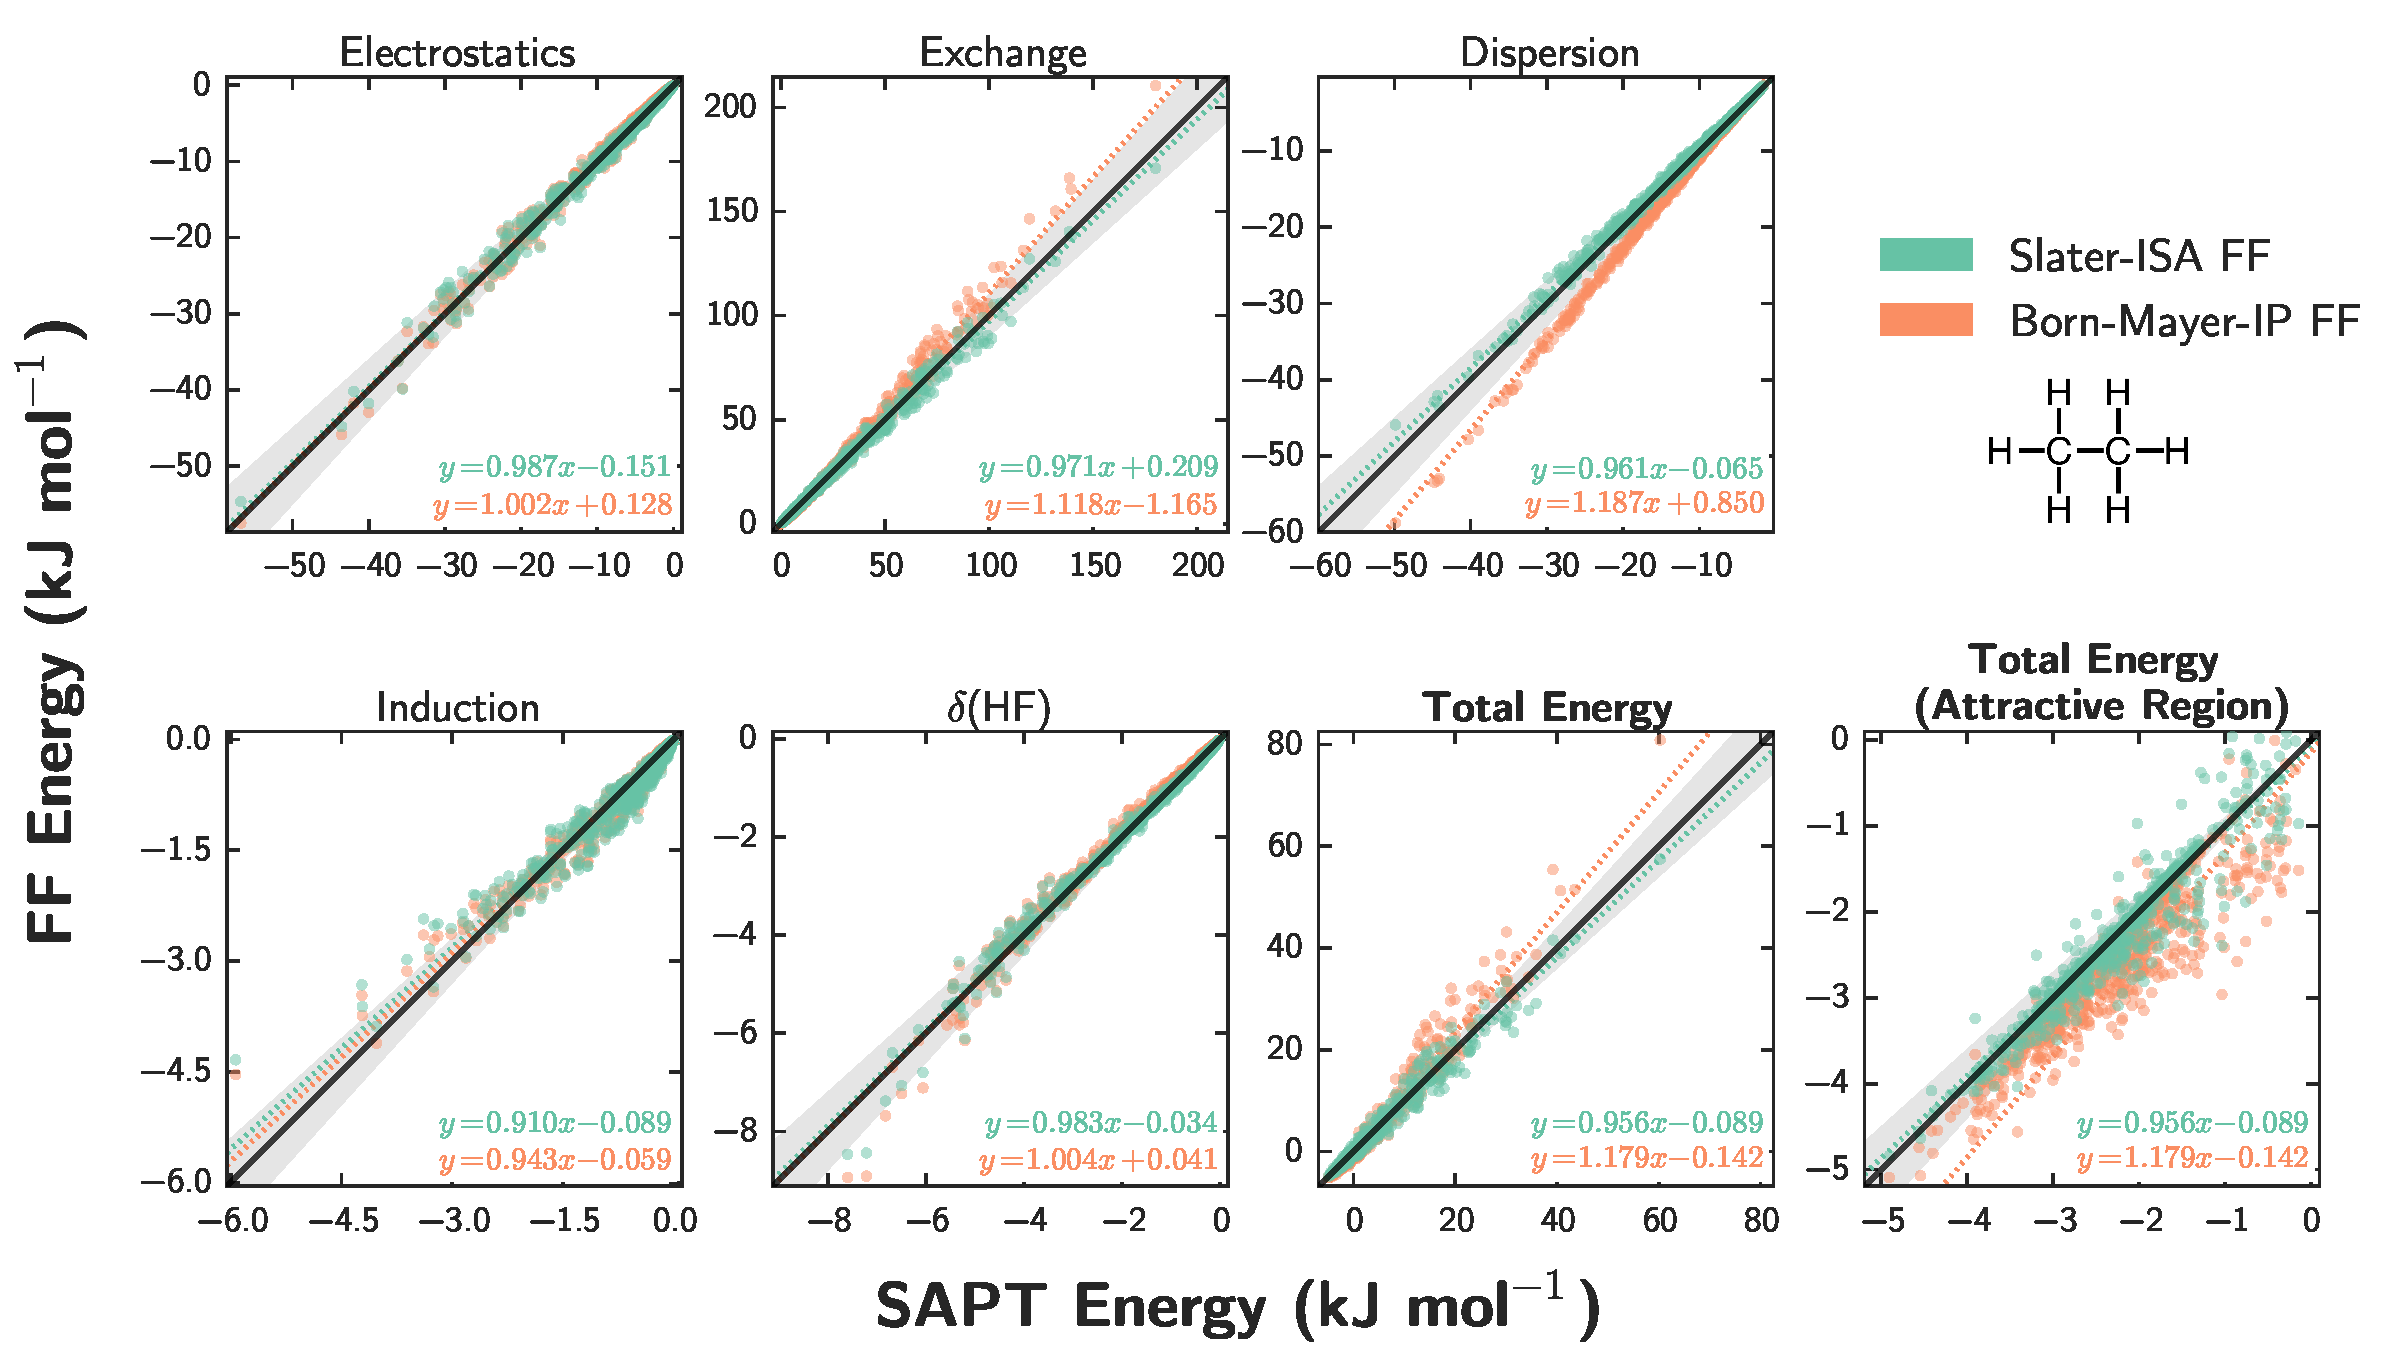
\includegraphics[width=0.9\textwidth]{isotropic/ethane_ethane_scatter.pdf}
    \caption{
    Force field fits for the ethane dimer using the Slater-ISA (green) and
    Born-Mayer-IP (orange) FFs.
    Fits for each energy component are displayed along with two views of the total interaction energy.
    The diagonal line (black) indicates perfect agreement between reference energies
    and each force field, while shaded grey areas represent points within $\pm
    10\%$ agreement of the benchmark. To guide the eye, a line of best fit (dotted
    line) has been computed for each force field and for each energy component.
     }
    \label{fig:isotropic-ethane-scatter}
    \end{figure}
    %%%%%%%% Ethane-Ethane Scatter %%%%%%%%%%

As with the argon dimer, for the ethane dimer the \isaffold produces more
accurate exchange and dispersion energies compared to the \saptff. Here, the
effects of the \isaffold for dispersion are even more pronounced, likely because
the conventional damping of the \saptff is systematically in error due to
differences in both the form of the damping function and exponents. As for the
total interaction energy, we again find that the \saptff exhibits large errors
for repulsive contributions, while the \isaffold naturally reproduces
interactions for both attractive and strongly repulsive configurations.  Even
in the attractive regime, the \saptff is systematically too attractive. These
systematic errors are the result of imperfect error cancellation
between the exchange and dispersion components of the fit, and are discussed in
more detail in Section \ref{sec:isotropic-results-robustness}. 

    %%%%%%%%%%% Ethane-Ethane PES %%%%%%%%%%%
    \begin{figure}
    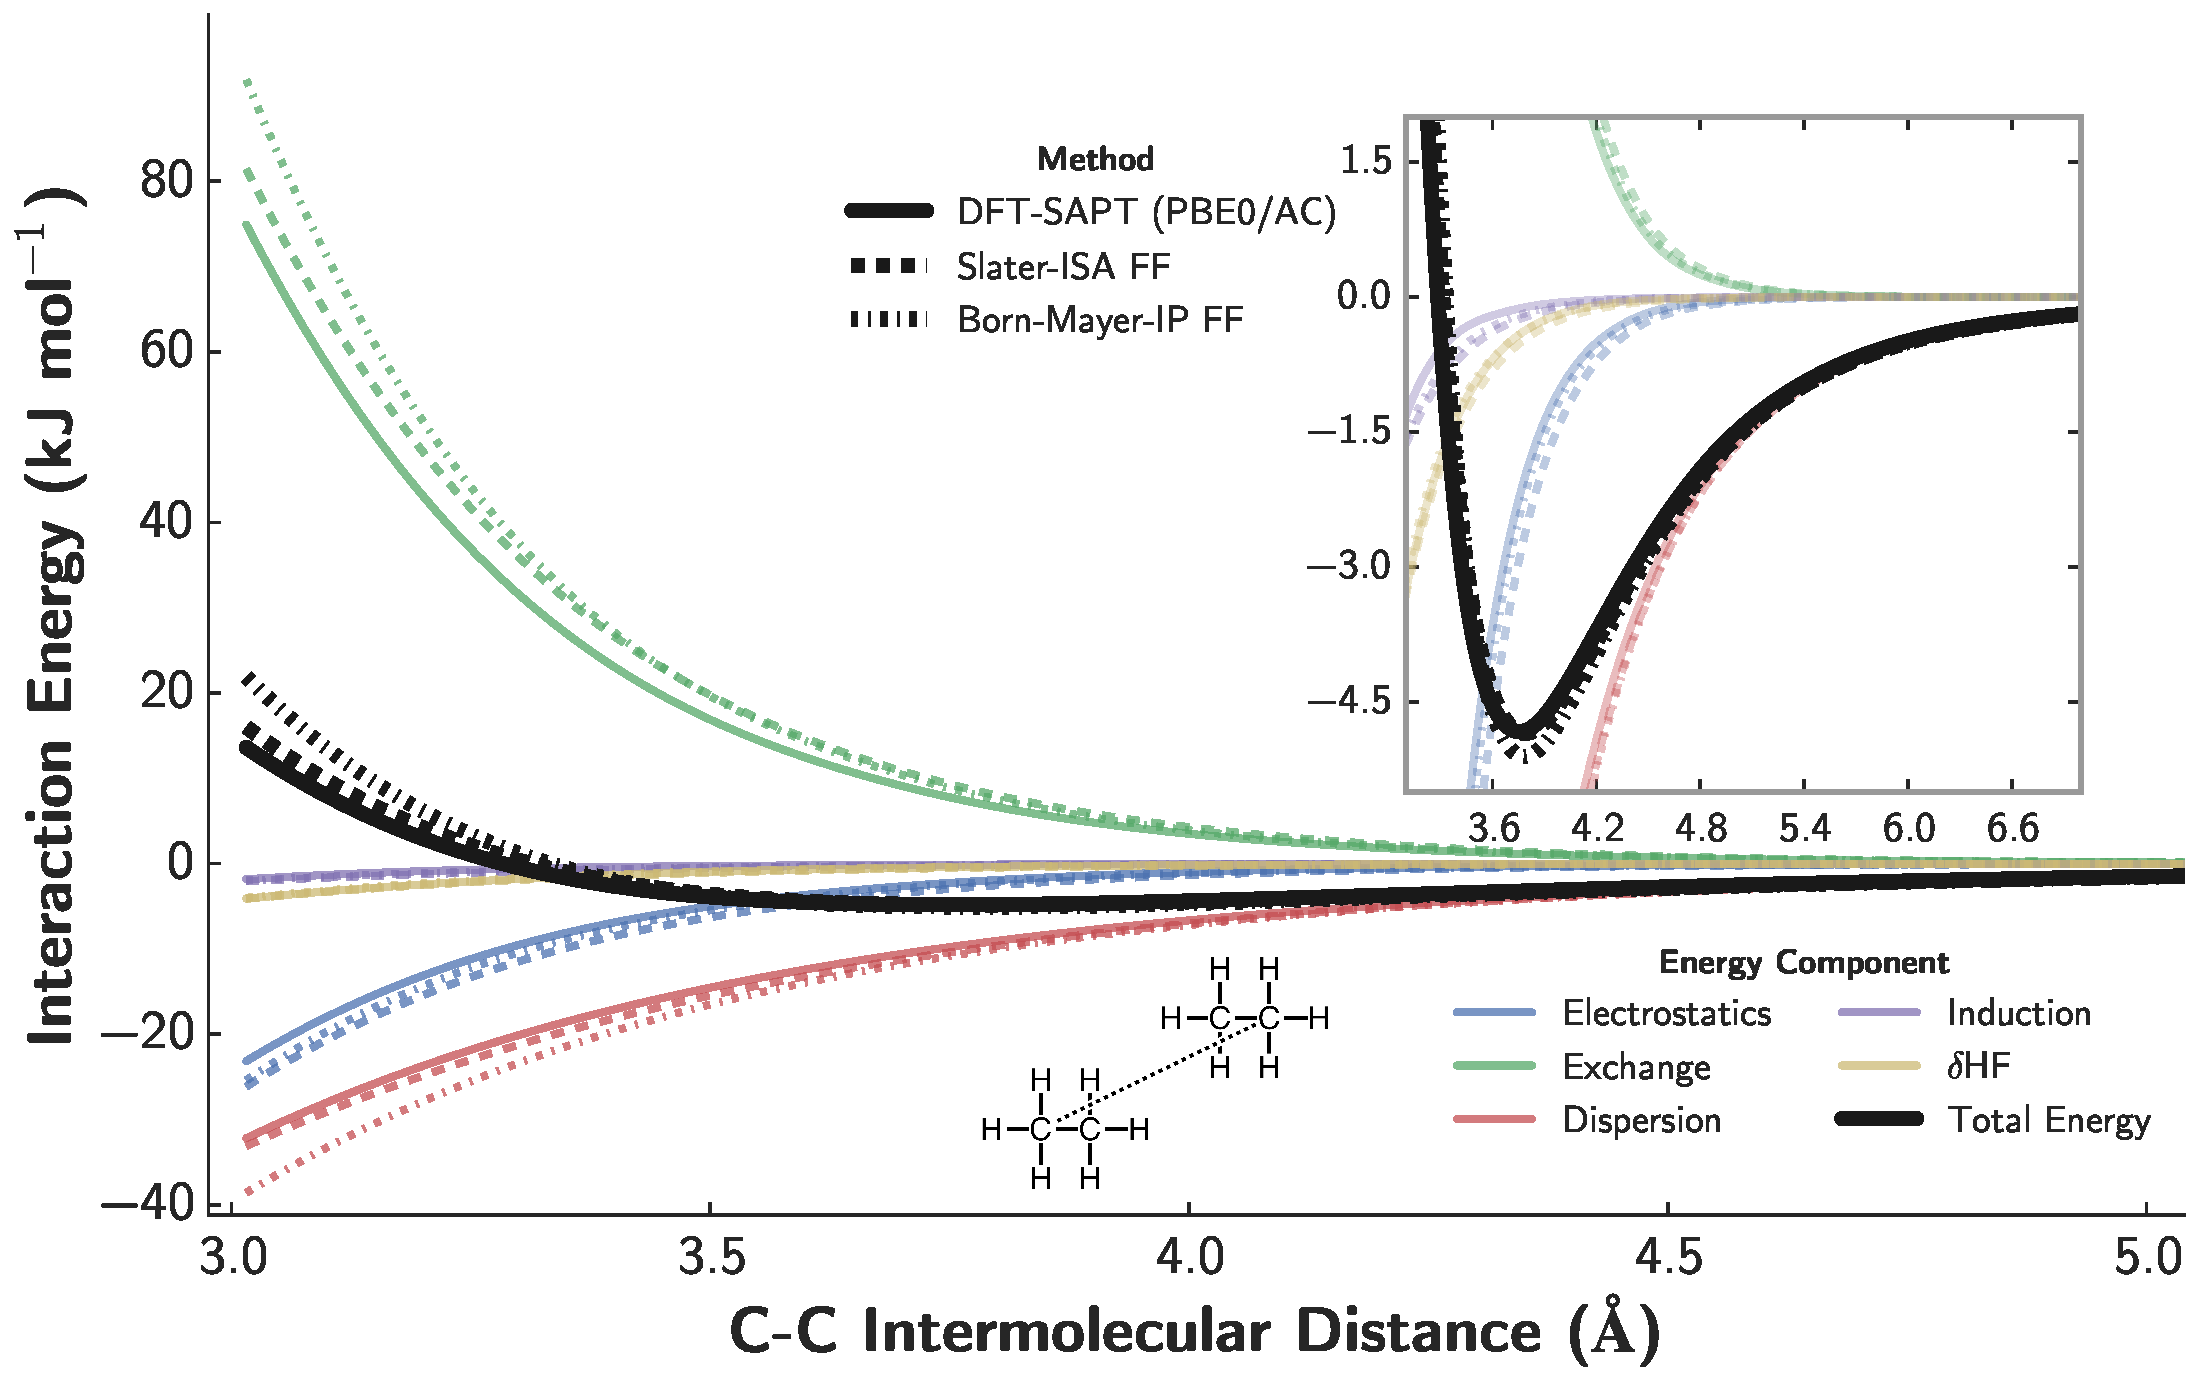
\includegraphics[width=0.9\textwidth]{isotropic/ethane_ethane_pes.pdf}
    \caption{
    A representative potential energy scan near a local minimum for the ethane dimer. 
    Interaction energies for the \isaffold (dashed curves) and the \saptff (dash-dotted
    curves) are shown alongside benchmark \saptpbeo energies (solid curves). The
    energy decomposition for DFT-SAPT and for each force field is shown for reference.
     The ethane dimer configuration in this scan corresponds to the most
    energetically attractive dimer included in the training set; other
    points along this scan are not included in the training set.
    }
    \label{fig:isotropic-ethane-pes}
    \end{figure}
    %%%%%%%%%%% Ethane-Ethane PES %%%%%%%%%%%

Examining a specific cut across the ethane-ethane PES
(\cref{fig:isotropic-ethane-pes}) visually confirms these results.  Both potentials do
an excellent job of reproducing the benchmark DFT-SAPT energies in the minimum
energy region, though the \saptff is slightly too attractive. (Other cuts of
the PES would show the Born-Mayer-IP predictions to be significantly more in error,
consistent with the scatter plots). Along the repulsive wall, however, the
\saptff predictions worsen in comparison to those from the \isaffold. Finally,
the PES shows an increased reliance on error cancellation between the
various energy components for the \saptff compared to the \isaffold.

As shown in the Supporting Information of \citen{VanVleet2016}, the Lennard-Jones force field models
are incapable of reproducing the entirety of the ethane PES; depending on the
weighting function, either the repulsive wall or the attractive well can be
reproduced, however no set of parameters can predict both regions
simultaneously.


\end{subsubsection}
\begin{subsubsection}{Acetone Dimer}

The acetone dimer provides a final interesting example involving a moderately sized
organic molecule.
From both the scatter plots (\cref{fig:isotropic-acetone-scatter}) and the PES cross section
(\cref{fig:isotropic-acetone-pes}), it is evident that both the Slater-ISA and
Born-Mayer-IP force fields do an
excellent job of reproducing DFT-SAPT energies for the low energy dimers.
Along the repulsive wall, however, the \saptff shows larger systematic
errors in each energy component, and seems to rely on error cancellation
to achieve good agreement in the total energy.
This reliance on error cancellation has two negative effects: 
Firstly, the additional scatter in the total energy of the \saptff
fit, especially prominent for attractive configurations, indicates that this
error cancellation is imperfect in certain cases. MSE
for the \isaffold ($-0.0115$ kJ mol$^{-1}$) are an order of magnitude lower than for
the \saptff ($0.182$ kJ mol$^{-1}$) in the attractive region of the potential.  Secondly,
as we shall later explore, reliance on error cancellation likely
contributes to the somewhat decreased transferability of the \saptff as
compared to the \isaffold. 

As shown in the Supporting Information of \citen{VanVleet2016}, the
\ljff predictions for acetone are reasonably good in both the tail and minimum
energy regions of the potential, however the \ljff grossly overpredicts the
\saptpbeo energies along the repulsive wall.

    %%%%%%% Acetone-Acetone Scatter %%%%%%%%%
    \begin{figure}
    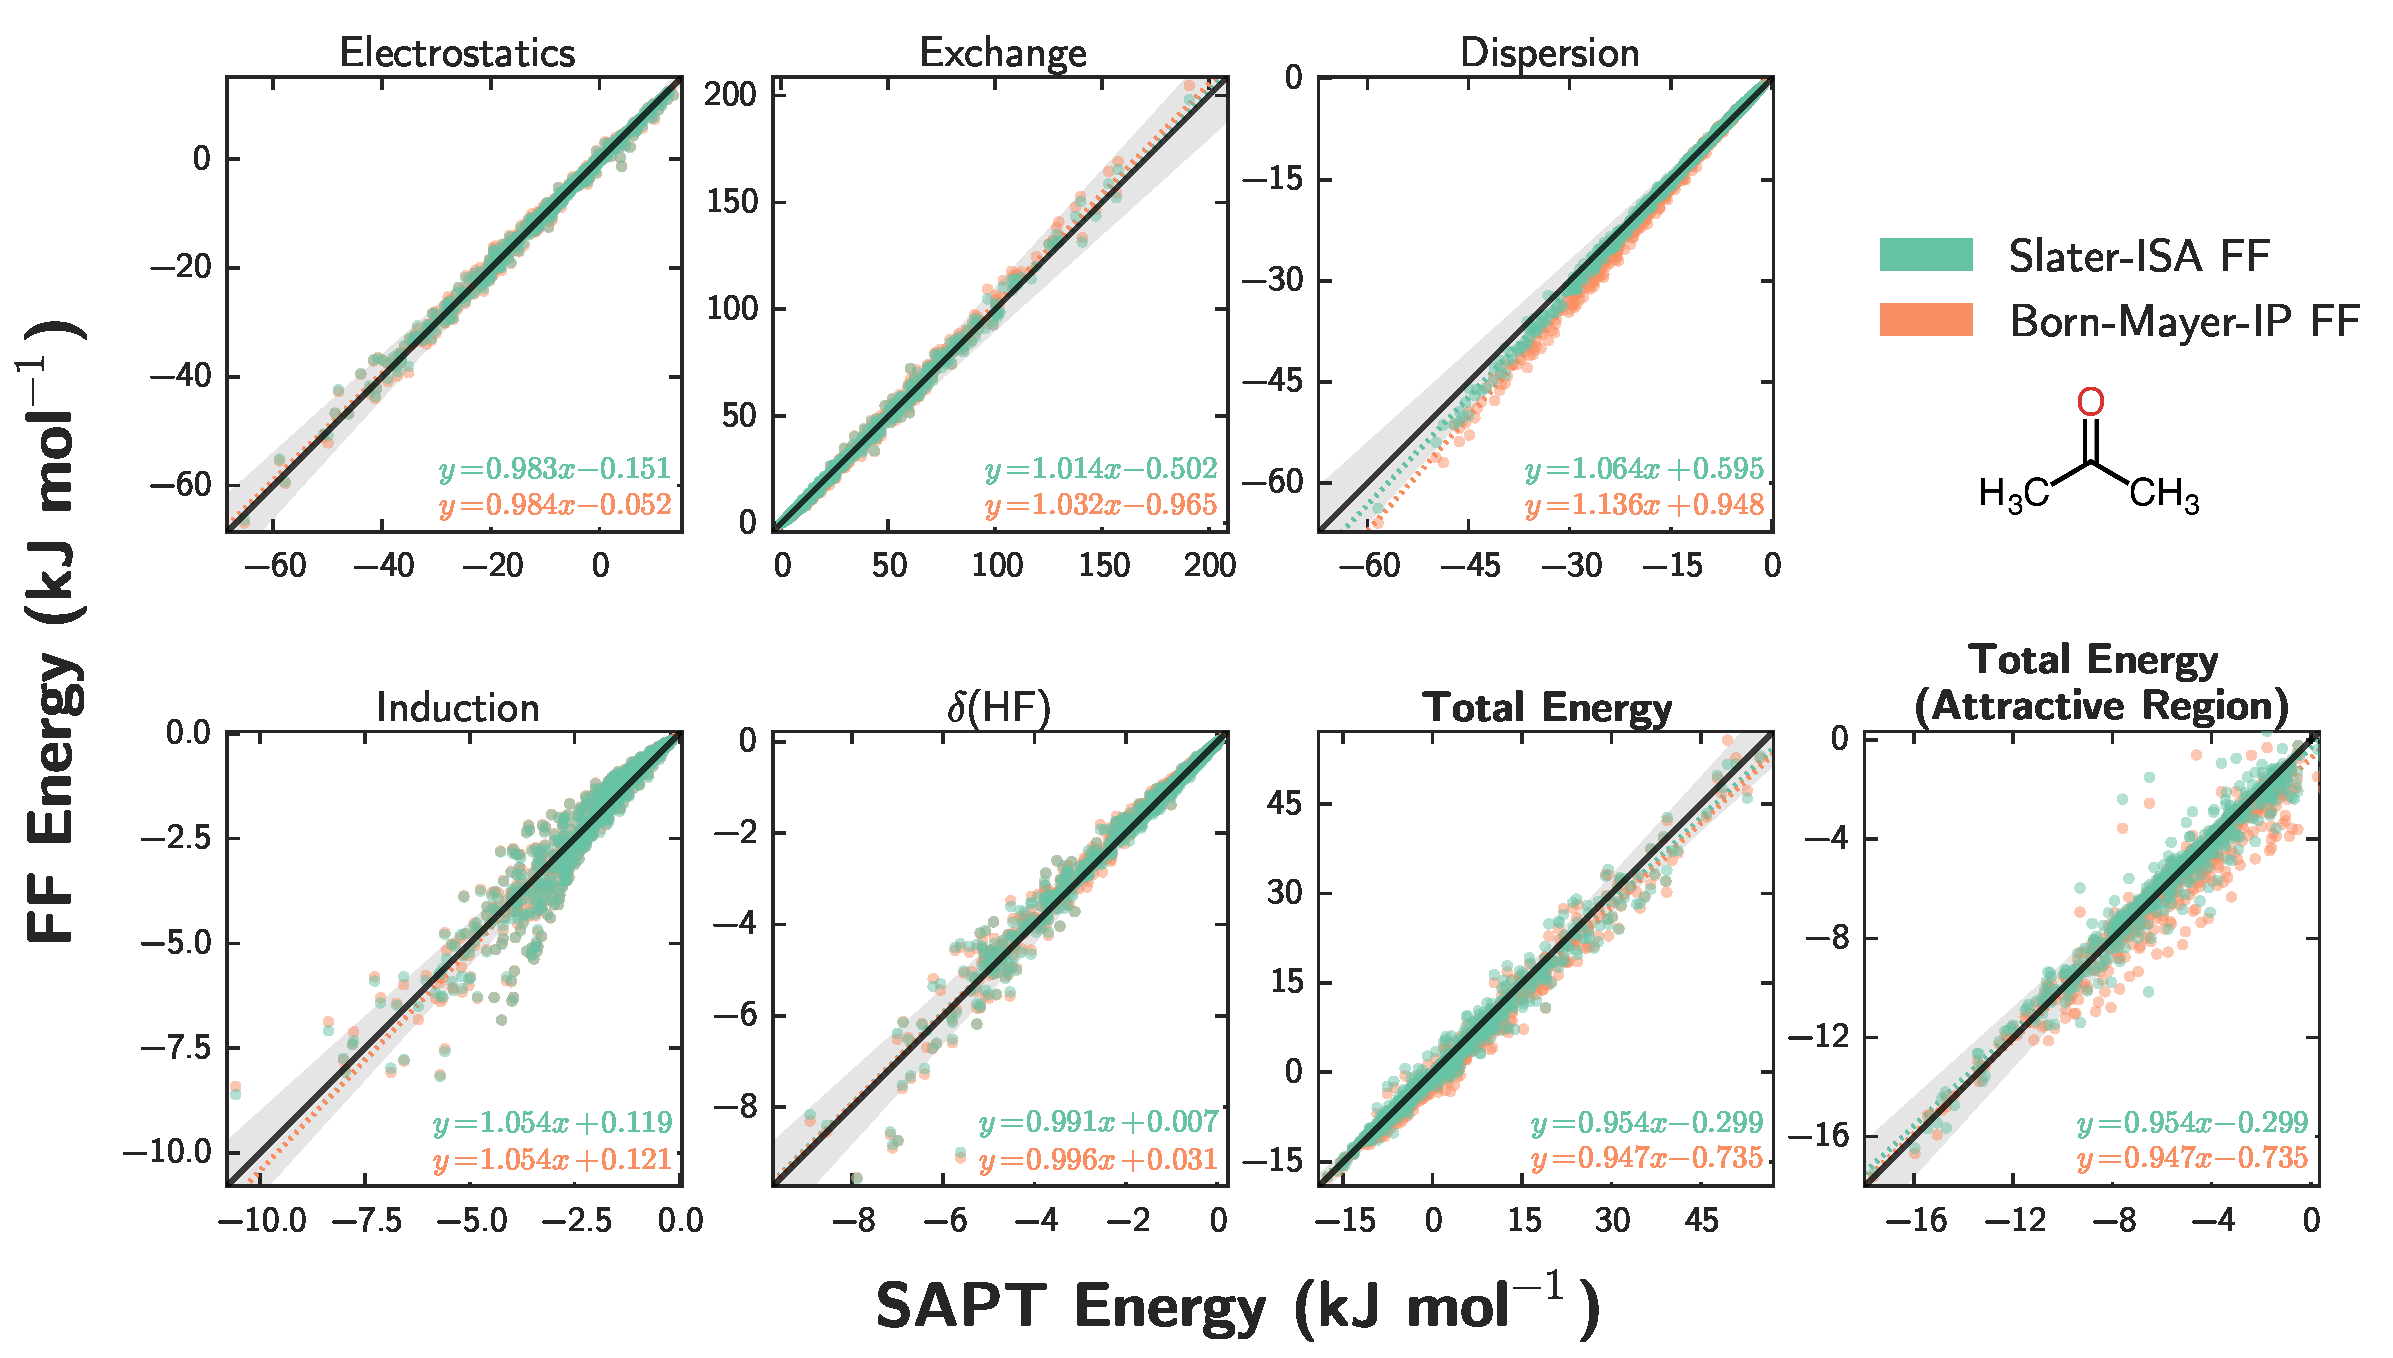
\includegraphics[width=0.9\textwidth]{isotropic/acetone_acetone_scatter.pdf}
    \caption{
    Force field fits for the acetone dimer using the Slater-ISA (green) and
    Born-Mayer-IP (orange) FFs, as in \cref{fig:isotropic-ethane-scatter}.
    %% Fits for each energy component are displayed along with two views of the total interaction energy.
    %% The diagonal line (black) indicates perfect agreement between reference energies
    %% and each force field, while shaded grey areas represent points within $\pm
    %% 10\%$ agreement of the benchmark. To guide the eye, a line of best fit (dotted
    %% line) has been computed for each force field and for each energy component.
            }
    \label{fig:isotropic-acetone-scatter}
    \end{figure}
    %%%%%%% Acetone-Acetone Scatter %%%%%%%%%


    %%%%%%%%%%% Acetone-Acetone PES %%%%%%%%%
    \begin{figure}
    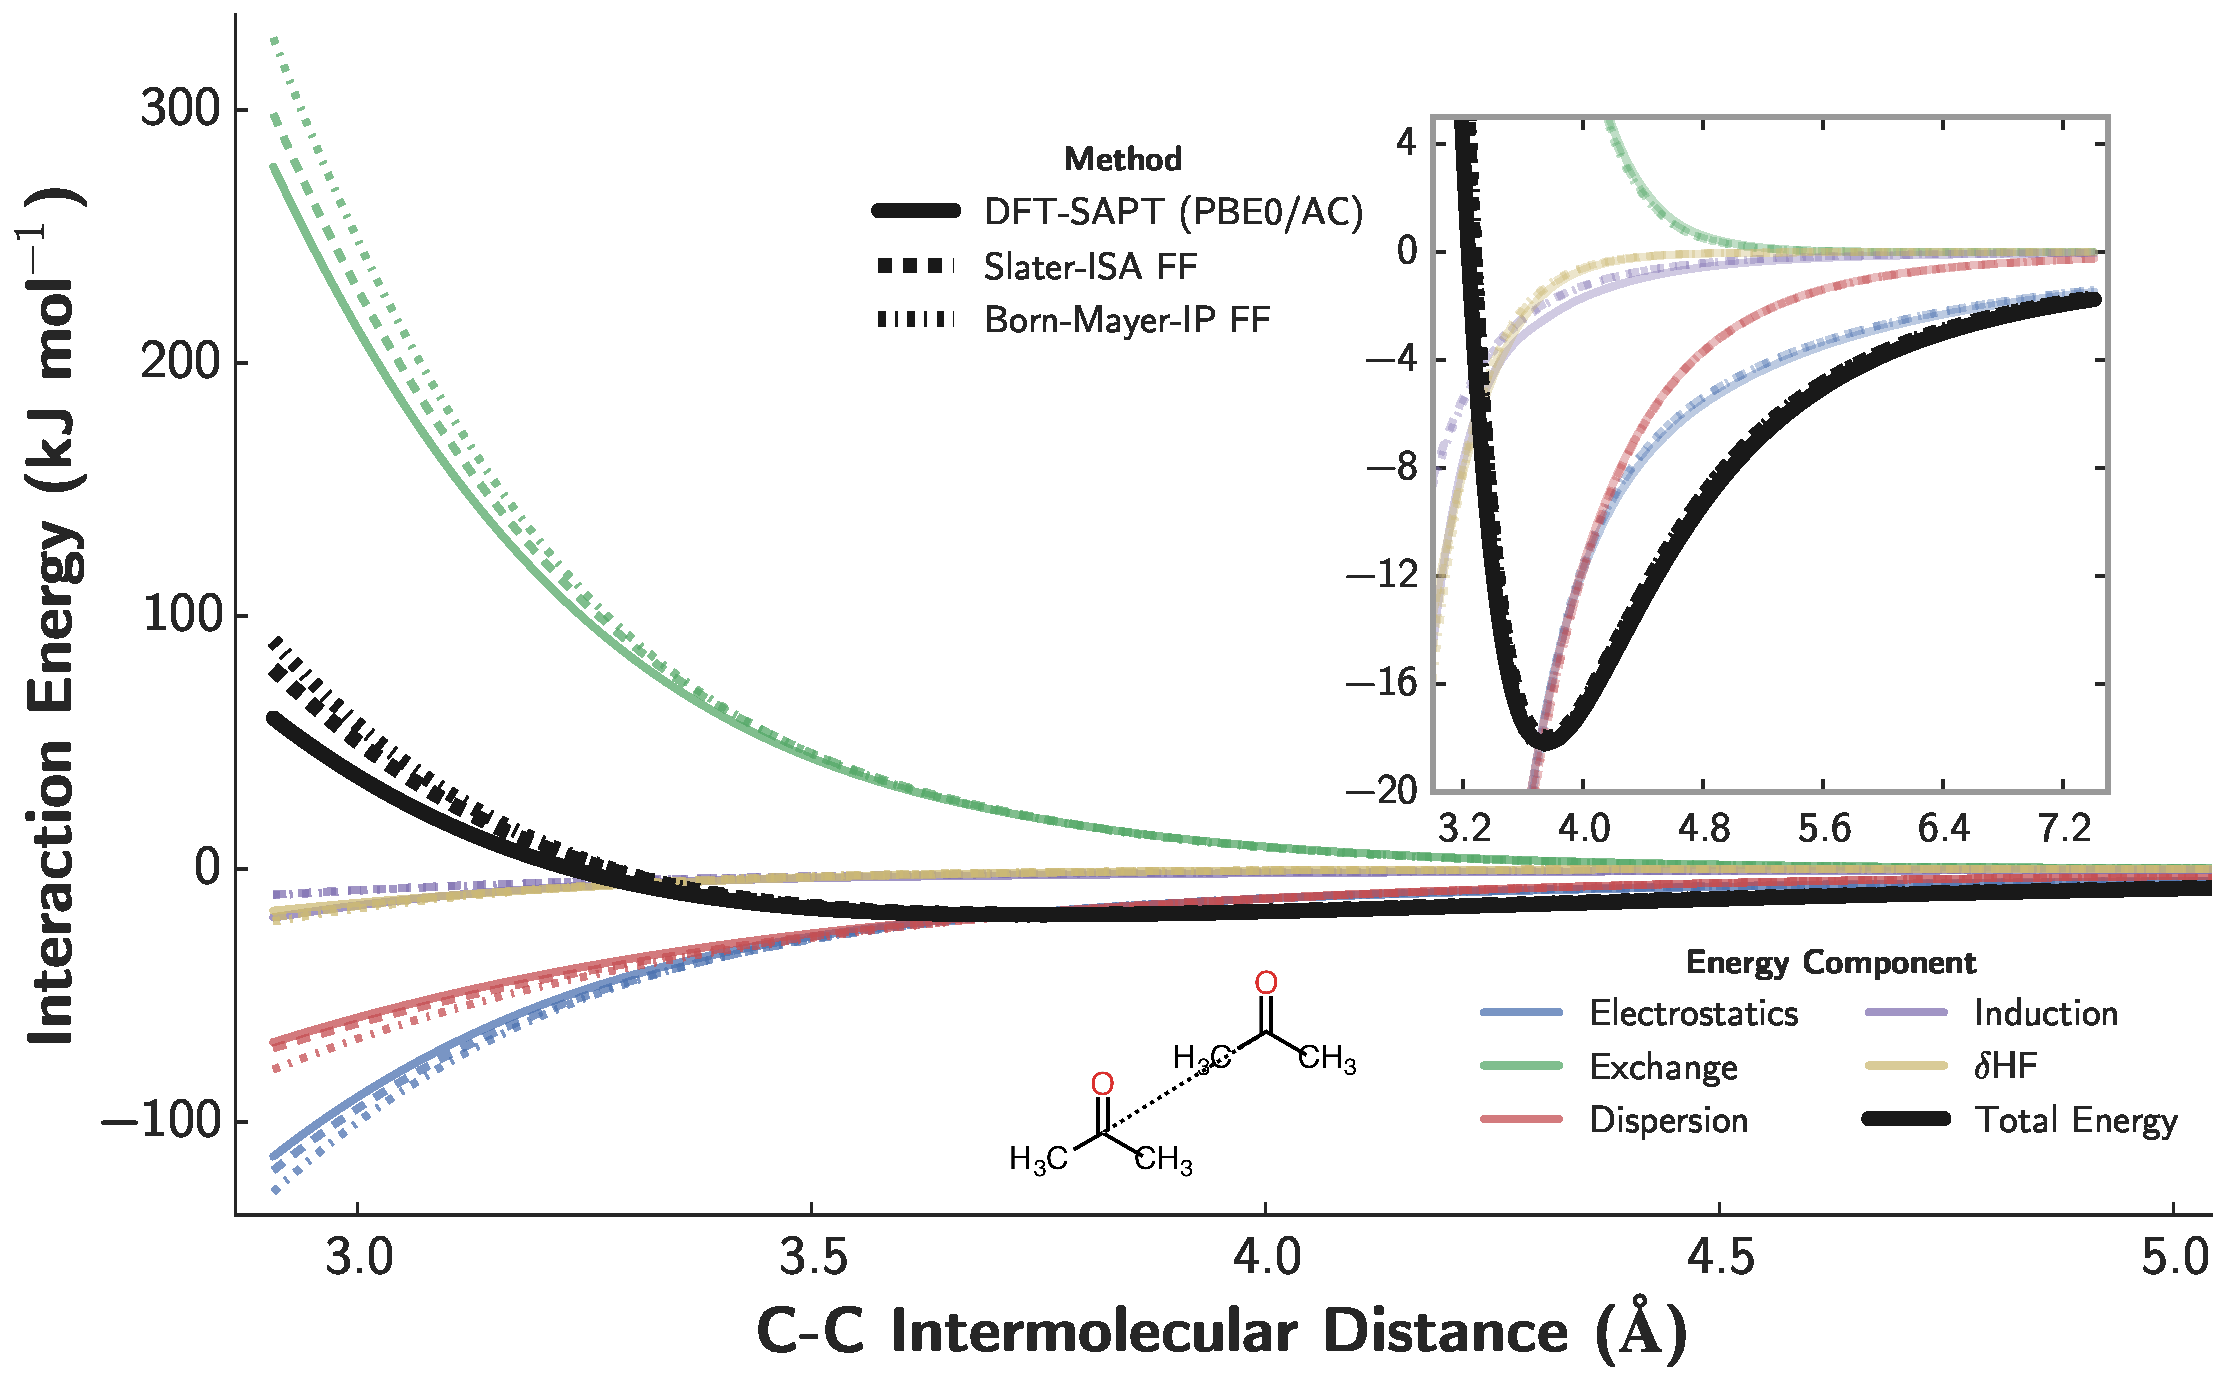
\includegraphics[width=0.9\textwidth]{isotropic/acetone_acetone_pes.pdf}
    \caption{
      A representative potential energy scan near a local minimum for the
      acetone dimer.  Interaction energies for the \isaffold (dashed curves) and
      the \saptff
      (dash-dotted curves) are shown alongside benchmark \saptpbeo energies (solid
      curves). The energy decomposition for DFT-SAPT and for each force field is
      shown for reference.  The intermolecular distance is taken to be the
      internuclear distance between the two carbonyl carbons on each acetone
      monomer.  The configuration in this scan corresponds to the
      most attractive dimer configuration included in the training set for the acetone dimer;
      other points along this scan have not explicitly been included in the training
      set.
      }
    \label{fig:isotropic-acetone-pes}
    \end{figure}
    %%%%%%%%%%% Acetone-Acetone PES %%%%%%%%%


\end{subsubsection}
\end{subsection}
\begin{subsection}{Accuracy: Comparison with experiment}
\label{sec:isotropic-accuracy_experiment}


    %%%%%%%%%%%% Ar-Ar Virial %%%%%%%%%%%%%%%
    \begin{figure}
    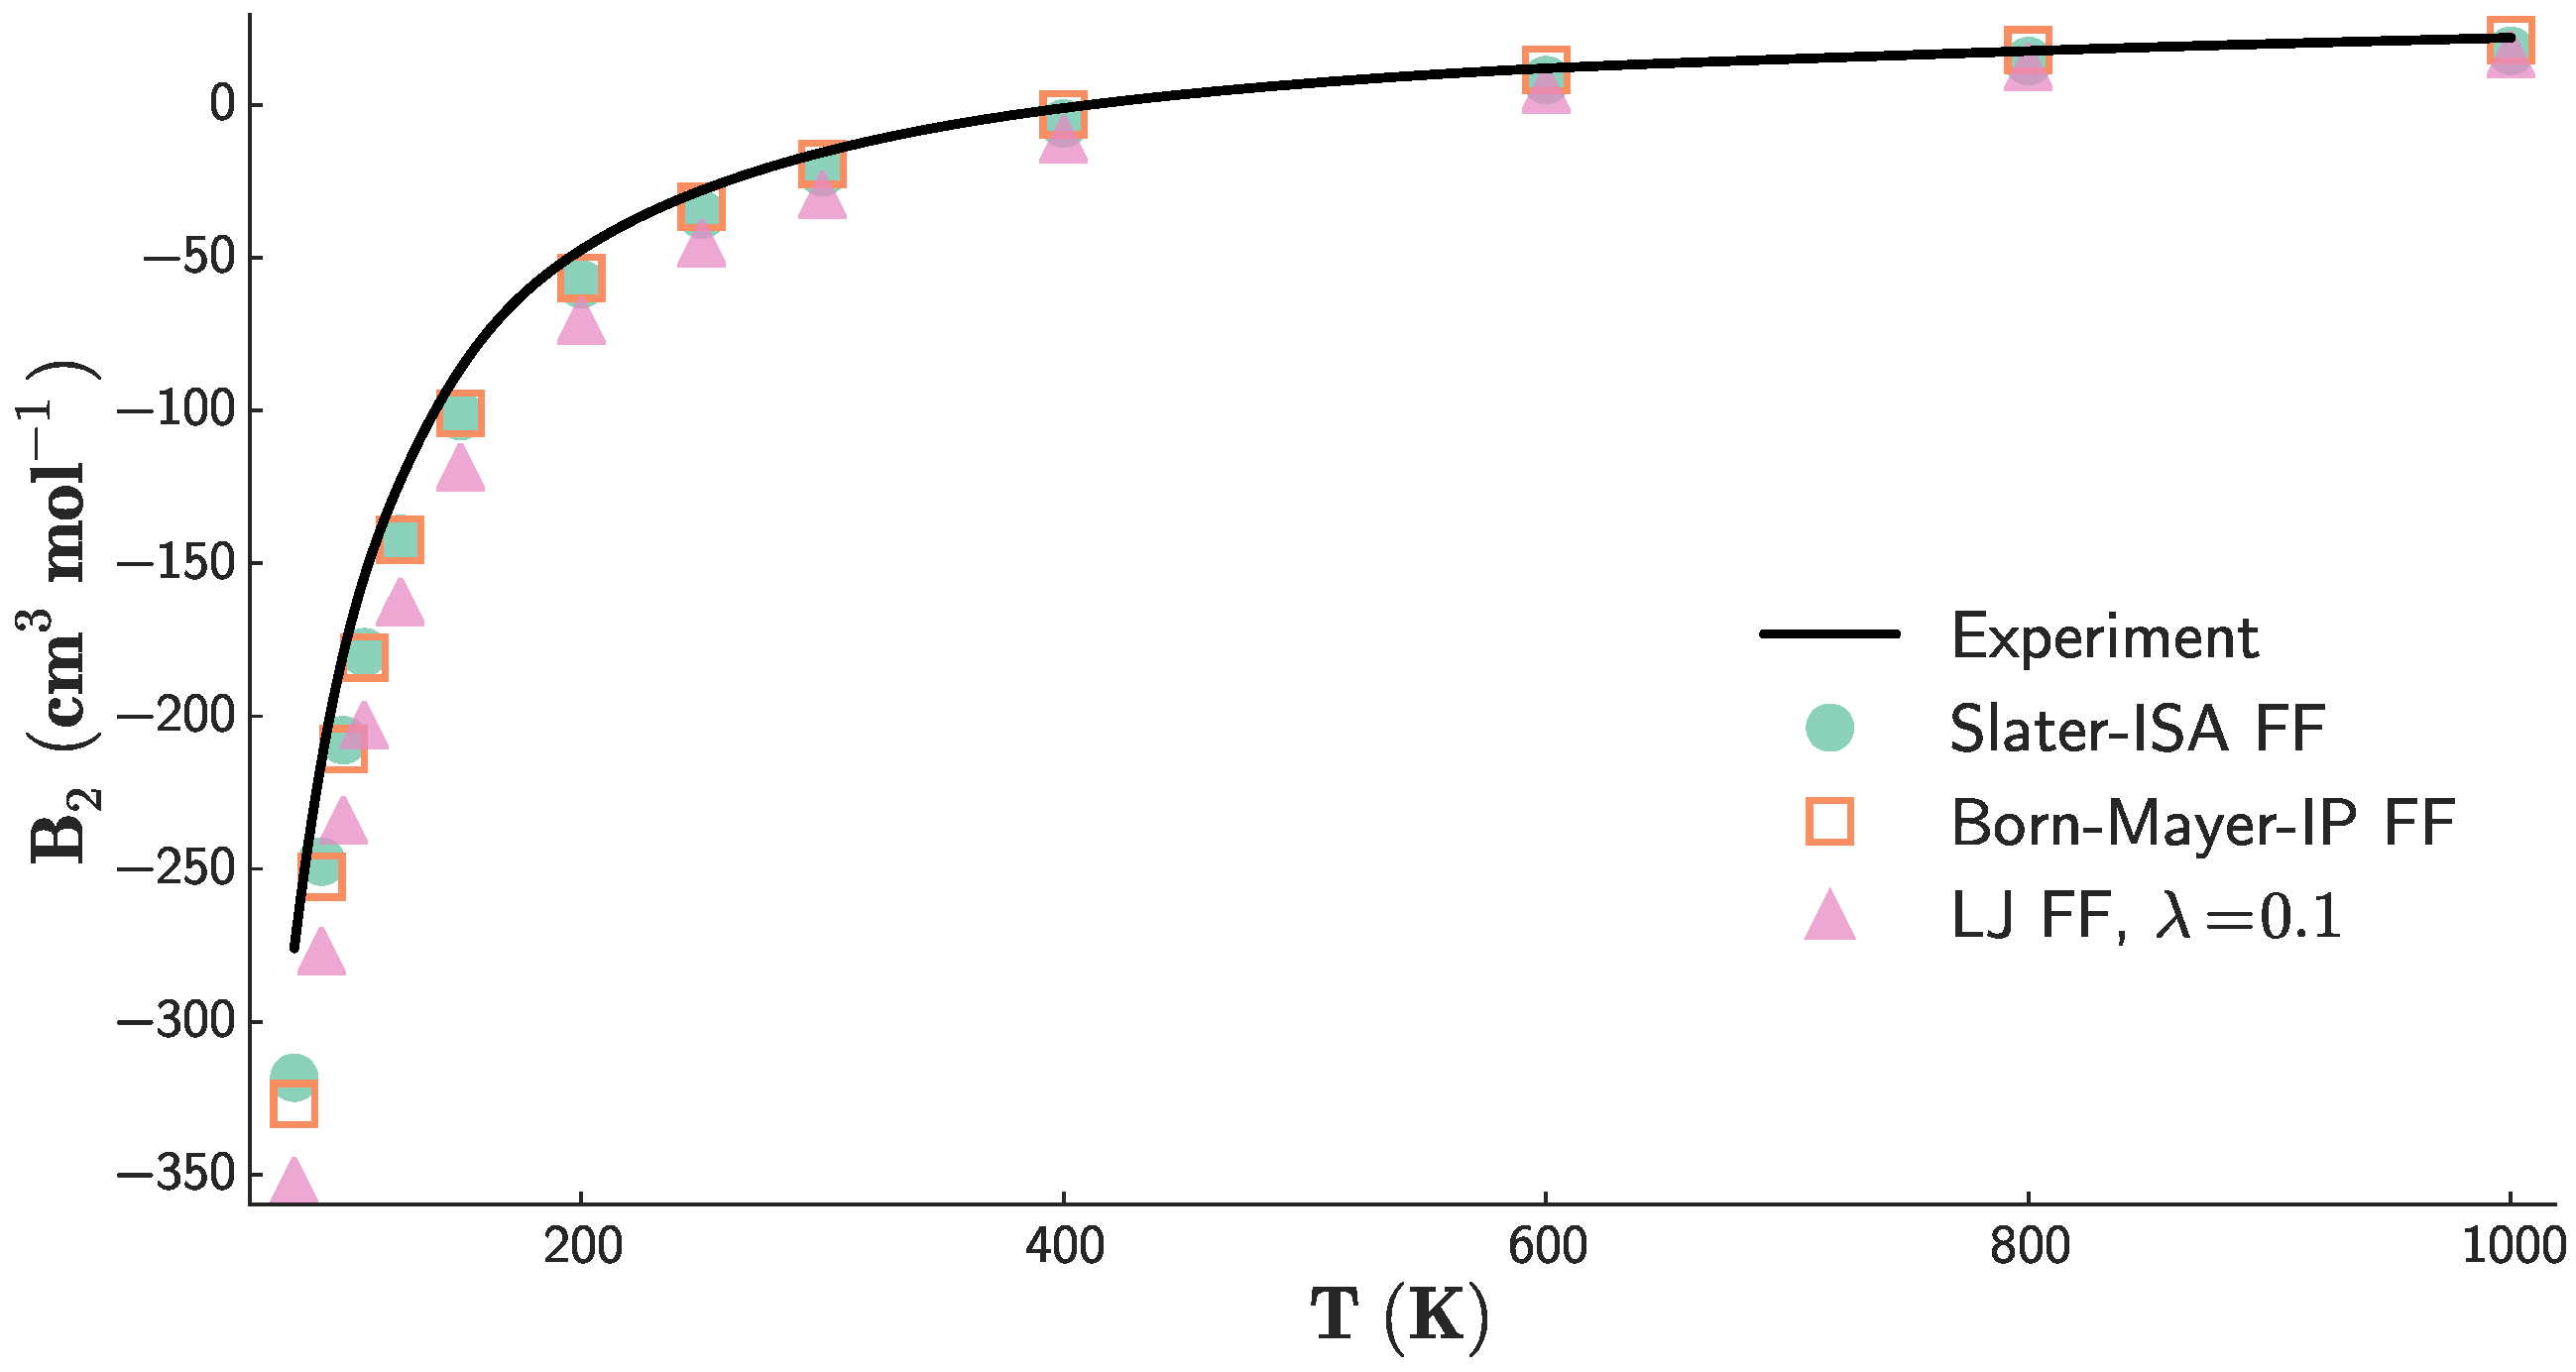
\includegraphics[width=0.9\textwidth]{isotropic/ar_2nd_virial_wi_lj.pdf}
   \caption{
    Second virial coefficients for argon. The Slater-ISA and the Born-Mayer-IP
    FFs are shown as green
    circles and orange squares, respectively; the black line corresponds to
    experiments from \citen{Dymond1980}.
           }
    \label{fig:isotropic-ar-virial}
    \end{figure}
    %%%%%%%%%%%% Ar-Ar Virial %%%%%%%%%%%%%%%

We have benchmarked the above force fields against experimental 
second virial coefficients and, in the case of ethane, enthalpies of
vaporization and liquid densities.
The classical 2\super{nd} virial coefficients were calculated for both argon and
ethane using rigid monomer geometries, following the procedure described in
\citen{McDaniel2013}. 
Enthalpies of
vaporization and liquid densities were calculated using the OpenMM molecular
simulation package
\cite{Eastman2013}
as described in \cref{sec:isotropic-methods}.
Higher-order multipole moments
--- which were negligible for these molecules --- were neglected, and so
only rank $0$ terms were used in these calculations. 
Results are shown in Figures \ref{fig:isotropic-ar-virial} and \ref{fig:isotropic-ethane-virial}
as well as \cref{tab:isotropic-deltah}.


For argon, since both \isaffold and \saptff accurately reproduce the energetics 
of low-energy configurations, it
is unsurprising that both force fields yield accurate virial
coefficients over a wide range of temperatures.  Errors in computed $B_2$
coefficients (for both potentials) are likely attributable to small errors in
the \saptpbeo potential itself,
\cite{Podeszwa2005a}
and, to a much lesser extent, the neglect of nuclear
quantum effects at lower temperatures.
\cite{Vogel2010}
Despite the good (in an RMSE sense) fit quality of the \ljff ($\lambda=0.1$),
this force field overpredicts the magnitude of the 2\super{nd} virial for argon, likely as a
result of the effective dispersion coefficient, which overestimates the
attraction in the tail
region of the PES (see Supporting Information of \citen{VanVleet2016}). Although it is certainly
possible to parameterize a Lennard-Jones model \emph{empirically} for argon,
such a force field would rely on a subtle cancellation of errors between the
minimum energy- and tail-regions of the PES. As the proper balance is
impossible to predict a priori, this result highlights one of the difficulties
of using the less physical LJ model in the development of ab-initio force
fields.

%
    %%%%%%%% Ethane-Ethane Virial %%%%%%%%%%%
    \begin{figure}
    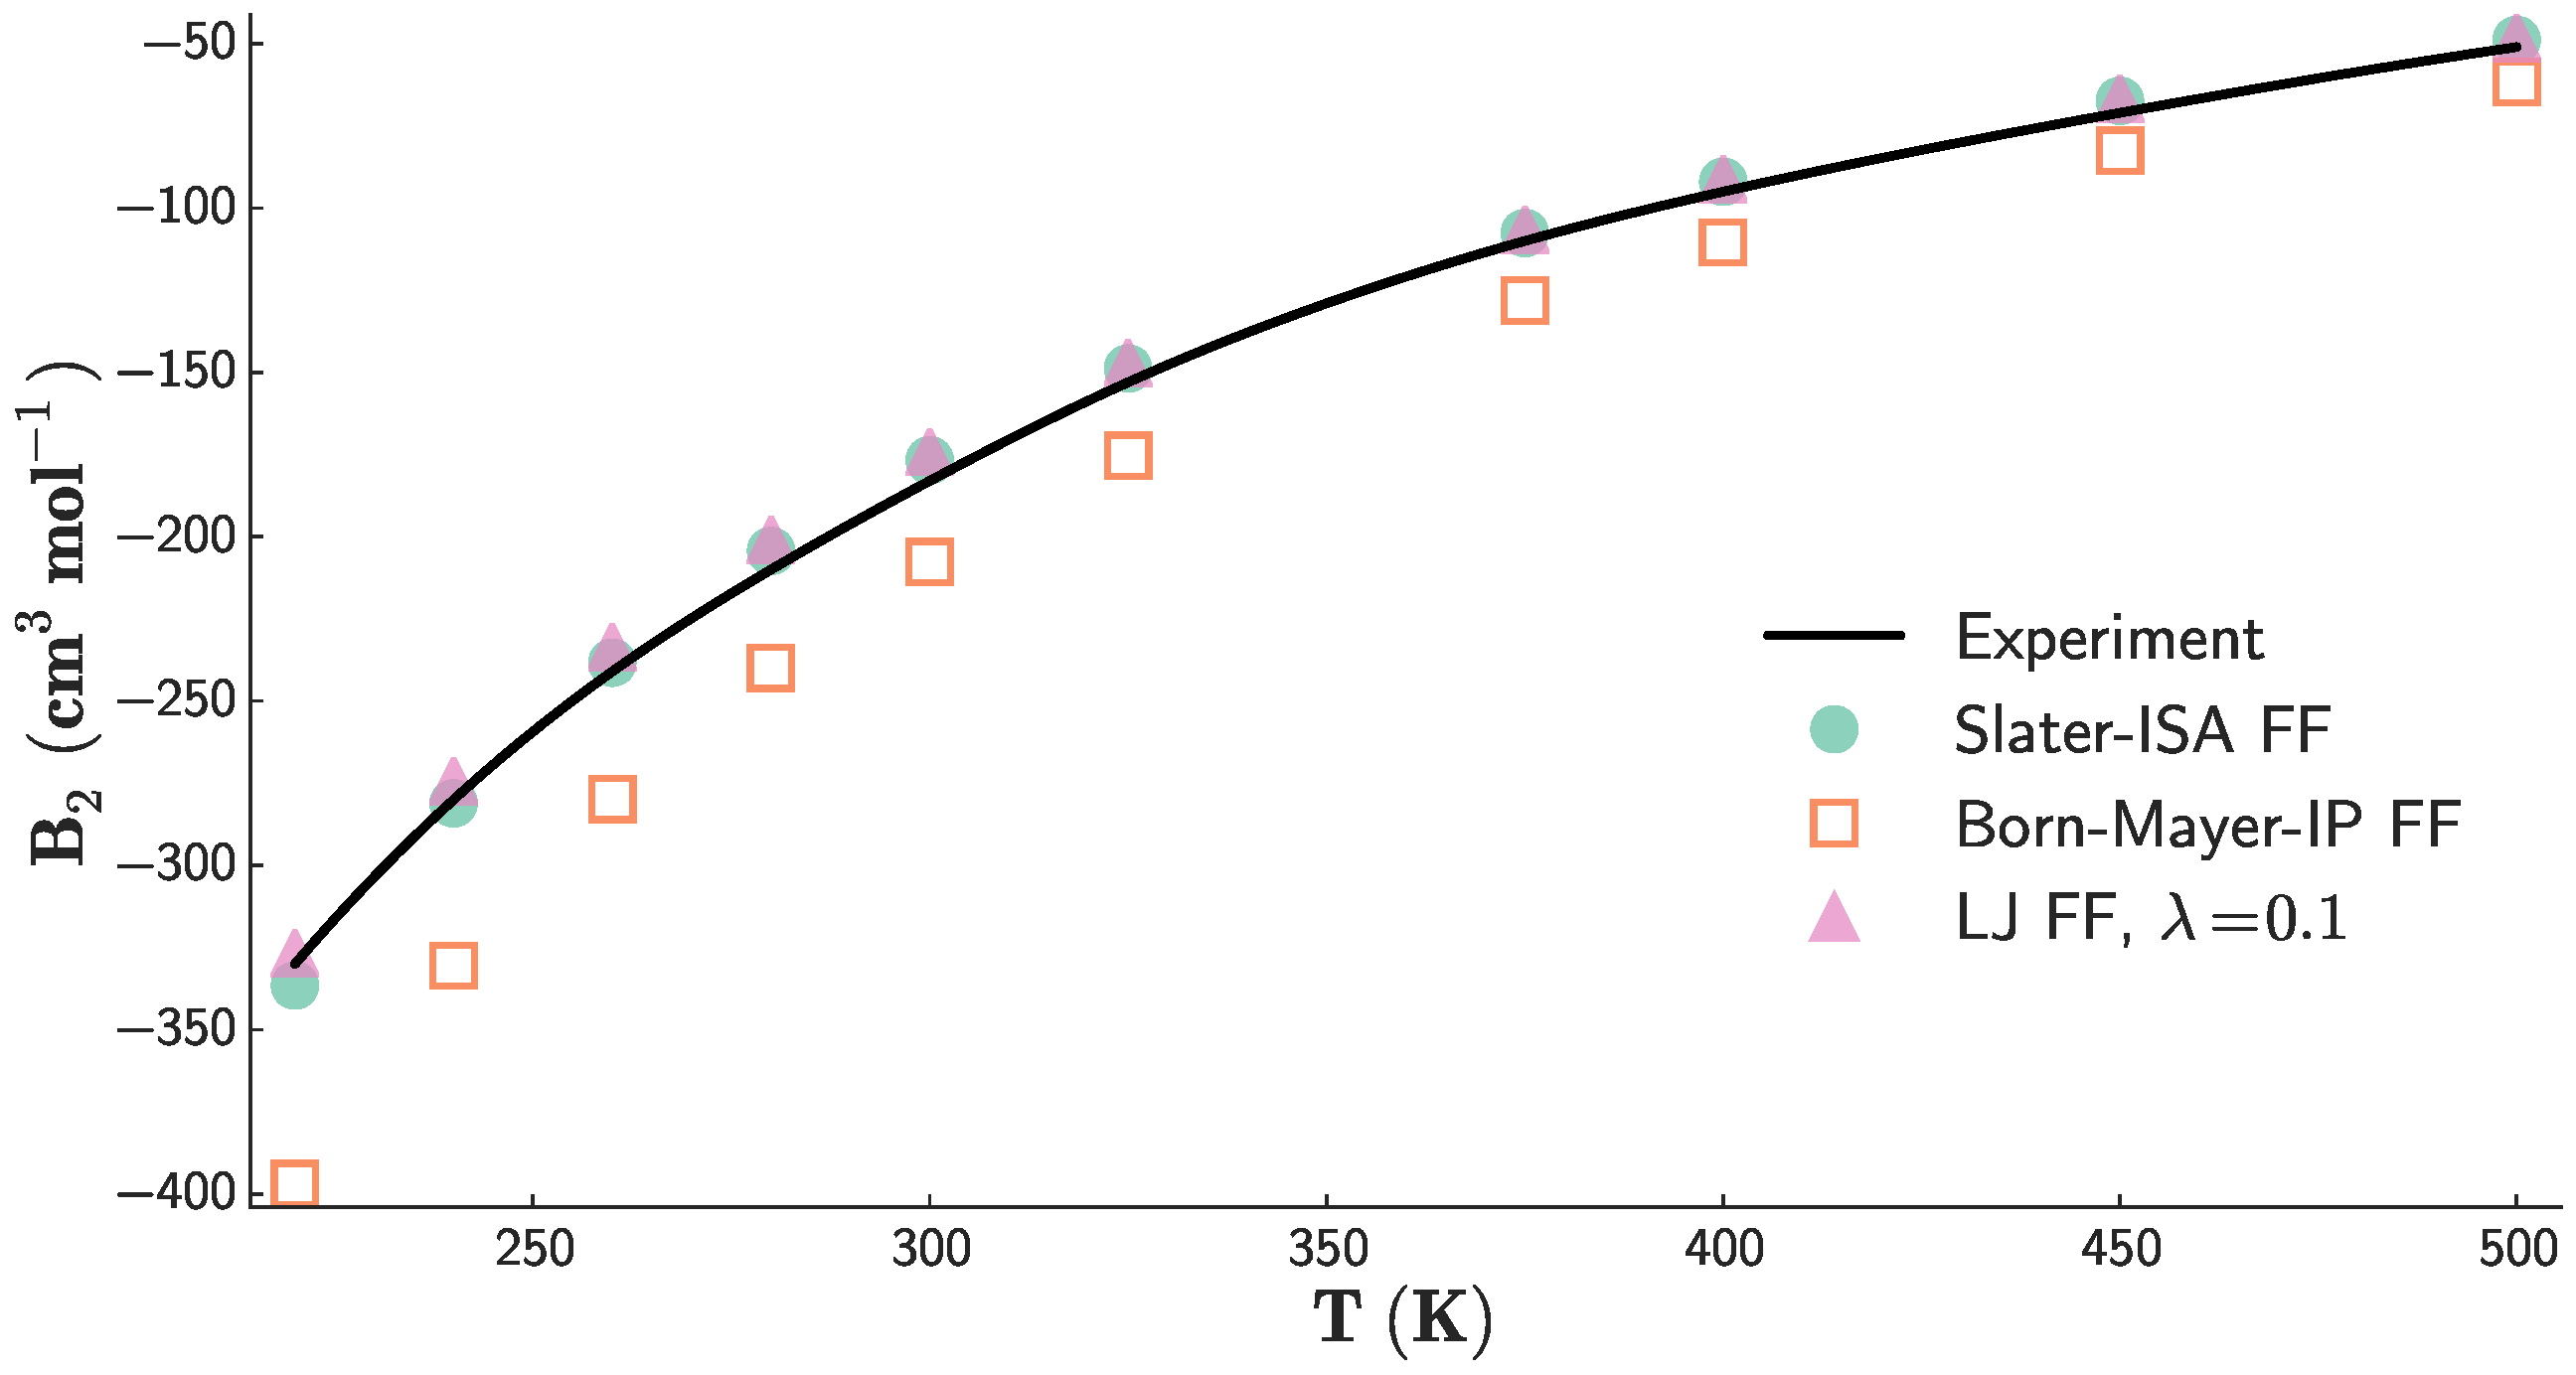
\includegraphics[width=0.9\textwidth]{isotropic/ethane_2nd_virial_wi_lj.pdf}
   \caption{
    Second virial coefficients for ethane. 
    The Slater-ISA and Born-Mayer-IP FFs are shown as green
    circles and orange squares, respectively; the black line corresponds to
    experiments from \citen{Dymond1980}.
    }
    \label{fig:isotropic-ethane-virial}
    \end{figure}
    %%%%%%%% Ethane-Ethane Virial %%%%%%%%%%%
%

In the case of ethane, the \isaffold is in excellent agreement with experiment,
whereas the \saptff underpredicts $B_2$ by as much as 20\%. These results are
indicative, not only of the more accurate functional form and parameterization
of \isaffold, but also of the high accuracy of the underlying \saptpbeo benchmark
energies. In this case, \ljff also correctly predicts the virial.  Using
weighting functions for each model that are optimal for the 91 dimer test set
as a whole ($\lambda = 2.0$ for the \isaffold and the \saptff,
$\lambda = 0.1$ for the \ljff), all force fields produce similar results for
$\Delta H_{\text{vap}}$ and $\rho$ (\cref{tab:isotropic-deltah}). These values are
slightly overestimated by all force fields (especially in the case of the
\saptff), which is to be expected given our neglect of many-body effects.
\citeauthor{McDaniel2014} have calculated the 3-body correction for the
\saptff; using this value as a global 3-body correction for all force fields,
we see that both the Slater-ISA and the Lennard-Jones force fields compare
very favorably to experiment, with the \isaffold perhaps slightly more accurate. 
%TO-DO: Update this once I have saptpbeo-ff results.

\end{subsection}

\begin{subsection}{Transferability}
\label{ss:transferability}

The transferability of interaction potentials is a crucial aspect of practical
molecular simulations. Here we examine `parameter transferability', by which
we mean the extent to which parameters from two homo-monomeric systems can
combined to predict the intermolecular interactions of the resulting mixed
hetero-monomeric system. 
As a measure of parameter transferability, we compared characteristic RMSE
and \mse relative to
the benchmark data for two different parameterization schemes.  For the
`Dimer-Specific Fits', \A parameters were obtained for each of the 91 dimer
pairs individually; these results are identical to those discussed in the
previous two subsections. In contrast, for the `Transferable Fits', the \A
parameters were fit to the 13 homonomeric dimer pairs and were re-used
(without any further optimization) to calculate energies for the 78 mixed
systems using the combination rules listed in \cref{sec:isotropic-FF-forms}.
Results for each parameterization scheme are shown in \cref{tab:isotropic-rmse}. 
From the RMSE and \mse from the competing schemes, 
we see excellent parameter transferability for all force fields studied. 
For the \isaffold, characteristic RMSE and \mse for each component increase by a very small
fraction upon constraining the fit; due to small error cancellation, errors in the
total energy actually \emph{decrease} somewhat with these constraints. 
(This is possible since the total energy is not directly fit.)
The \saptff also displays a significant degree of transferability, though
errors in the total energy increase slightly upon constraining the fit.
As in prior work, the observed parameter transferability for both force fields can be
attributed to our use of a term-by-term parameterization scheme
(\cref{sec:isotropic-FF-forms}),
which serves to minimize error cancellation between energy components and generate a
more physically-meaningful (and thus transferable) set of parameters.
\cite{McDaniel2013,McDaniel2012a}
Finally, note that for four of the five interaction energy components the relative
change in RMSE on constraining the fit is smaller for the \isaffold than
the \saptff. The \dhf term is the exception, but even here the relative 
change in errors from the two methods are comparable. This suggests that the
\isaffold may be the more transferable of the force fields studied.
Nevertheless, the Lennard-Jones model is surprisingly transferable,
likely in part due to the same accurate and transferable `long-range'
electrostatics and polarization as the \isaffold. The non-polarizable, point-charge
Lennard-Jones model (results for which are shown in the Supporting
Information of \citen{VanVleet2016}) displays the least transferability (in both an RMSE and \mse
sense) of all force fields studied.

Although we do not examine it here, we expect that the previously demonstrated success\cite{McDaniel2013, McDaniel2012,
McDaniel2012a, McDaniel2014} of the \saptff with respect to `environment transferability'
--- the extent to which a single set of parameters can model a variety of phases and
molecular environments --- and `atom type transferability' --- the extent to which
atoms in chemically similar environments can accurately be grouped together
into `types' and treated using one parameter set --- 
would also apply to, or even be improved by, \isaffold. These issues are under
investigation in our groups.

\end{subsection}
\begin{subsection}{Robustness}
\label{sec:isotropic-results-robustness}


One of the practical challenges of ab initio force field development is the
robustness of the resulting force field quality with respect to the choice of an
appropriate training set and/or weighting function.  To this end, the default
weighting function (\cref{eq:isotropic-weighting-function}, $\lambda = 2.0$) was varied
to produce unconstrained fits that were skewed either towards attractive
($\lambda = 0.5$) or repulsive ($\lambda = 5.0$) configurations, and pairwise
differences in force field total energies were computed between each weighting
scheme. Characteristic root-mean-square pairwise differences (RMSD) between
each weighting function are shown in
\cref{tab:isotropic-rmsd-weightings}; as before, `attractive RMSD' were
calculated by excluding repulsive points from consideration. Note that, on
average, the default $\lambda = 2.0$ weighting scheme is optimal (in an RMSE
sense) for both the Slater-ISA and Born-Mayer-IP FFs.

Overall, both the \saptff and the \ljff display significant weighting function
sensitivity. This sensitivity is not surprising; as both force fields are
unable to reproduce the entirety of the potential energy surface, changing the
weighting scheme (or equivalently, the balance of configurations in the
training set) alters the parameters in the \saptff or the \ljff models quite 
substantially. Even excluding repulsive configurations, RMSD
of $\sim0.5$ kJ mol$^{-1}$ are typical for the \saptff. RMSD are
somewhat smaller for the \ljff ($\sim0.3$ kJ mol$^{-1}$), however
qualitatively we see that differences in computed force field energies are systematic: smaller weighting
functions capture the minimum energy region of the potential while
overestimating the magnitudes of both the repulsive and tail regions of the
potential, whereas larger weighting functions tend to underestimate the
minimum energy region in order to correctly reproduce the repulsive wall.
Consequently, the Lennard-Jones model shows weighting-function sensitivity in
a manner that is not entirely captured by the RMSD, but is instead
reflected in the greater sensitivity of the \ljff (as compared to the \saptff)
in the prediction of experimental properties (\emph{vide infra}).
 
Note that for practical force field development (as opposed to minimization of
overall RMSE), the default weighting scheme for the \saptff
and the \ljff is suboptimal for many dimers in the test set.  Because both the
\saptff and the \ljff must inherently compromise between accuracy near the
minimum and along the repulsive wall, the weighting function requires
system-specific fine-tuning in order to achieve proper balance. This
empiricism creates significant challenges in the development of ab initio force
fields.

%%%%%%%%%%%%%%%%%%%%% Average RMSD Table %%%%%%%%%%%%%%%%%%%%%%%%%%%%%%%%%%%
\begin{table}[t]
\footnotesize
\centering
\renewcommand\arraystretch{1.1}
\begin{tabular}{@{}rcccccc@{}}
\hline
\toprule
\multirow{2}{*}{Characteristic RMSD} & \phantom{ab} &
  {$\lambda = 0.5$ vs 2.0} & \phantom{ab} &
  {$\lambda = 0.5$ vs 5.0} & \phantom{ab} &
  {$\lambda = 2.0$ vs 5.0} \\
  & \phantom{ab} &
  (kJ mol$^{-1}$) & \phantom{ab} &
  (kJ mol$^{-1}$) & \phantom{ab} &
  (kJ mol$^{-1}$) \\
\midrule
\isaffold    & & 0.742 (0.207) & & 0.990 (0.273) & & 0.306 (0.086) \\
\saptff   & & 1.866 (0.409) & & 2.632 (0.550) & & 0.797 (0.153) \\
\ljff  & & 1.301 (0.216) & & 1.605 (0.309) & & 0.324 (0.099) \\
%\midrule
%\addlinespace                                                                                                           
\bmsisaff & & 0.611 (0.178) & & 0.810 (0.236) & & 0.293 (0.081) \\ 

\bottomrule
\hline
\end{tabular}
\caption{
    Characteristic RMS pairwise differences (RMSD) in force field total energies 
    for different weighting functions with $\lambda$ values as defined in
    \cref{eq:isotropic-weighting-function}; values shown are the (arithmetic mean,
    rather than geometric)
    RMSD across the 91 dimer test set.
    Characteristic `Attractive' RMSD (as defined
    in \cref{tab:isotropic-rmse}) are shown in parentheses to the right of each overall RMSD.
	}
\label{tab:isotropic-rmsd-weightings}
\end{table}
\normalsize
%%%%%%%%%%%%%%%%%%%%% Average RMSD Table %%%%%%%%%%%%%%%%%%%%%%%%%%%%%%%%%%%

By contrast, we find the \isaffold to be robust with respect to the choice of
weighting function due to its more balanced treatment of repulsive and
attractive regions of the potential energy surface.
Average RMSD for the \isaffold are between two to three \emph{times} smaller compared
to the \saptff, and the \isaffold is relatively insensitive to the choice of
weighting function. 
These conclusions hold for both attractive and overall RMSD.
As a result, the Slater-ISA model largely eliminates the need for empirical
fine-tuning of the weighting function, which in turn greatly simplifies the
parameterization process and allows for a more robust prediction of chemical
and physical properties. 

For the ethane dimer, \cref{fig:isotropic-ethane-weighting} shows overall
force field energies for both the Slater-ISA and Born-Mayer-IP FFs for three
weighting functions. Results for the Lennard-Jones models are shown in the SI,
and are qualitatively similar to the \saptff results.
The \saptff fits vary qualitatively with $\lambda$, leading to a relatively large
uncertainty in calculated $B_2$ coefficients, enthalpies of vaporization, and
liquid densities (see \cref{tab:isotropic-deltah}). 
By skewing the fits towards attractive
configurations ($\lambda = 0.5$), the majority of attractive configurations
are predicted without systematic error, though points along the repulsive wall
(including those with net negative energies) are systematically too repulsive. 
Using a scheme which more heavily weights repulsive configurations, the \saptff
regains semi-quantitative accuracy for repulsive configurations, albeit at the expense
of a systematic increase in errors for the attractive dimer configurations.
Finally, we reiterate that the optimal weighting function for the
ethane dimer (here $\lambda = 0.5$ best reproduces the 2\super{nd} virial for
the \saptff) is
by no means universal for the molecules in the 91 dimer test set.

%%%%%%%%%%%%%%%%%%%%% Macroscopic Properties %%%%%%%%%%%%%%%%%%%%%%%%%%%%%%%%%%
\begin{table}
\small
\centering
\renewcommand\arraystretch{1.1}
\begin{tabular}{@{}rcccccc@{}}
\hline
\toprule
& \phantom{} &
  \multicolumn{4}{c}{Weighting Function} \\
\cmidrule{3-6} 

Force Field && $\lambda = 0.1$ &  $\lambda = 0.5$ &  $\lambda = 2.0$ &
$\lambda = 5.0$ & Experiment\\
%&& (default for \ljff)  &             &  (default for \isaffold and \saptff)   & \\

\midrule
\addlinespace
\multicolumn{7}{c}{\textbf{$\boldsymbol{\Delta H_{\text{vap}}}$ (kJ mol\super{-1});
$\boldsymbol{\rho = 0.546}$ g L\super{-1}, $\boldsymbol{T=184}$ K}} \\
%\addlinespace
%% \isaffold  && & 15.28 (14.65) & 15.34 (14.71) & 15.20 (14.57) & \multirow{3}{*}{14.7}\\
%% \saptff && & 15.08 (14.46) & 16.55 (15.92) & 18.59 (17.96) & \\
%% \ljff   && 15.50 (14.87) & 14.56 (13.94) & 11.36 (10.73) & 10.15 ( 9.52) & \\
\isaffold  && 15.3 (14.7)  & 15.3 (14.6) & 15.3 (14.7) & 15.2 (14.6) & \multirow{3}{*}{14.7}\\
\saptff && 14.3 (13.7)  & 15.1 (14.5) & 16.6 (15.9) & 18.6 (18.0) & \\
\ljff   && 15.5 (14.9)  & 14.6 (13.9) & 11.4 (10.7) & 10.1 ( 9.5) & \\
%
\addlinespace
\multicolumn{7}{c}{\textbf{$\boldsymbol{\rho}$ (g L\super{-1}); 
$\boldsymbol{P = 1}$ atm, $\boldsymbol{T=184}$ K}} \\
%\addlinespace
\isaffold  && 0.600 (0.566) & 0.602 (0.568) & 0.600 (0.566) & 0.593 (0.559) & \multirow{3}{*}{0.546} \\
\saptff && 0.521 (0.487) & 0.567 (0.533) & 0.632 (0.598) & 0.678 (0.644) & \\
\ljff   && 0.607 (0.573) & 0.610 (0.576) & 0.555 (0.521) & 0.494 (0.460) \\
\bottomrule
\hline
\end{tabular}
\caption{
    Enthalpies of vaporization and liquid densities for ethane as a function
    of force field and weighting function. Values in parentheses include an
    estimation of the 3-body correction (0.628 kJ mol\super{-1} and 0.034
    g mL\super{-1} for the enthalpy of vaporization and liquid density,
    respectively) as computed in \citen{McDaniel2014}. Experimental data taken
    from \citen{Witt1937} and \citen{Riddick1986}.
	}
\label{tab:isotropic-deltah}
\end{table}
\normalsize
%%%%%%%%%%%%%%%%%%%%% Macroscopic Properties %%%%%%%%%%%%%%%%%%%%%%%%%%%%%%%%%%


    %%%%%%%% Weighting Function Tests %%%%%%%
    \begin{figure}
        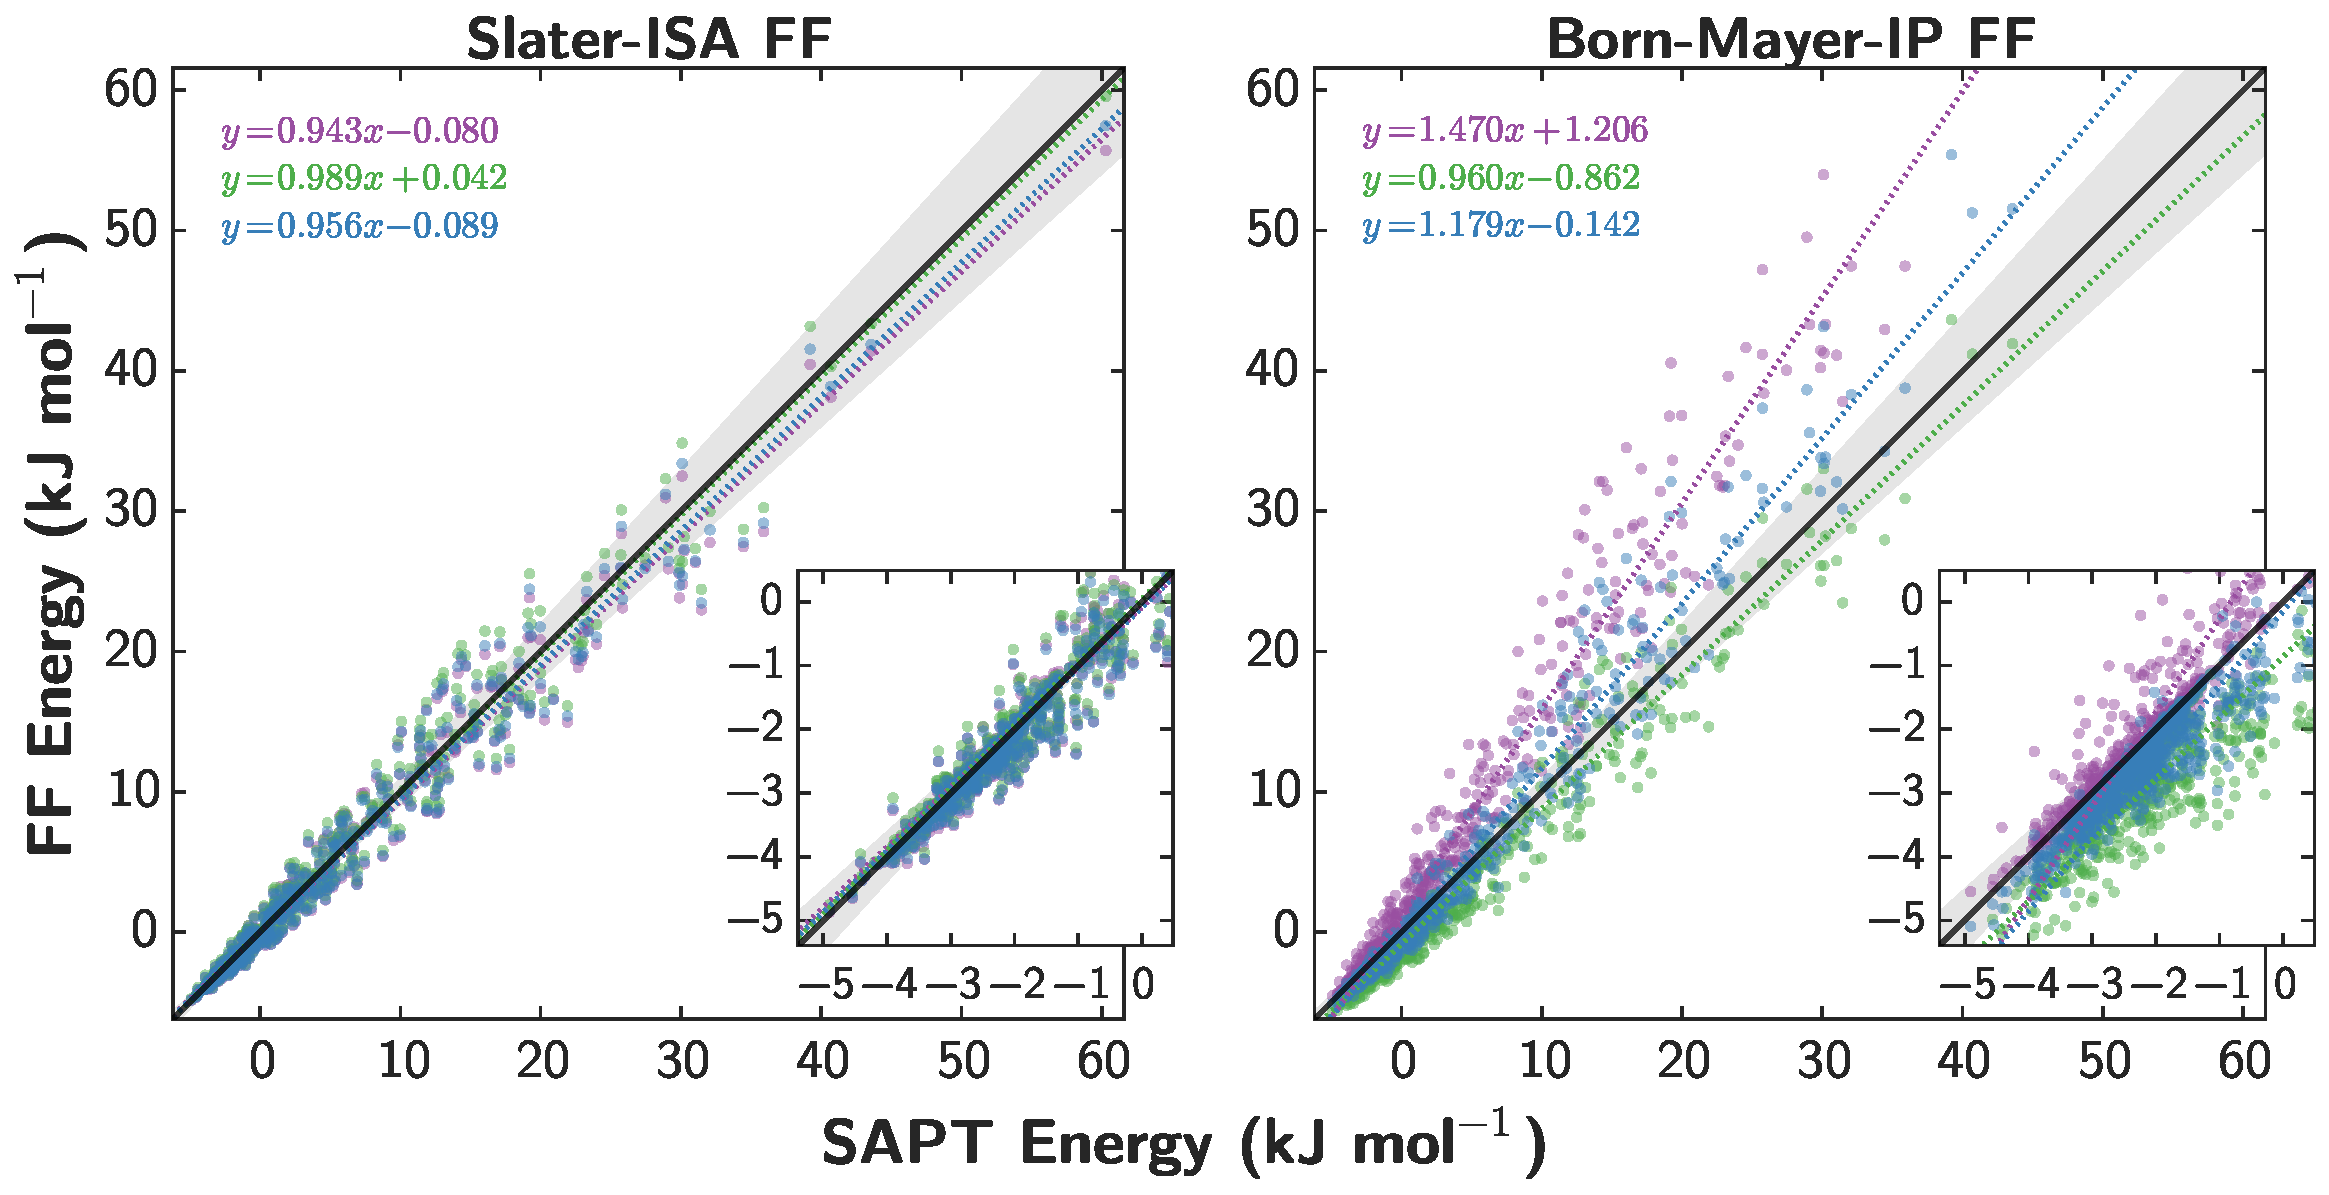
\includegraphics[width=0.9\textwidth]{isotropic/compare_ethane_ethane_scatter.pdf}
      \vfill
      \vfill
        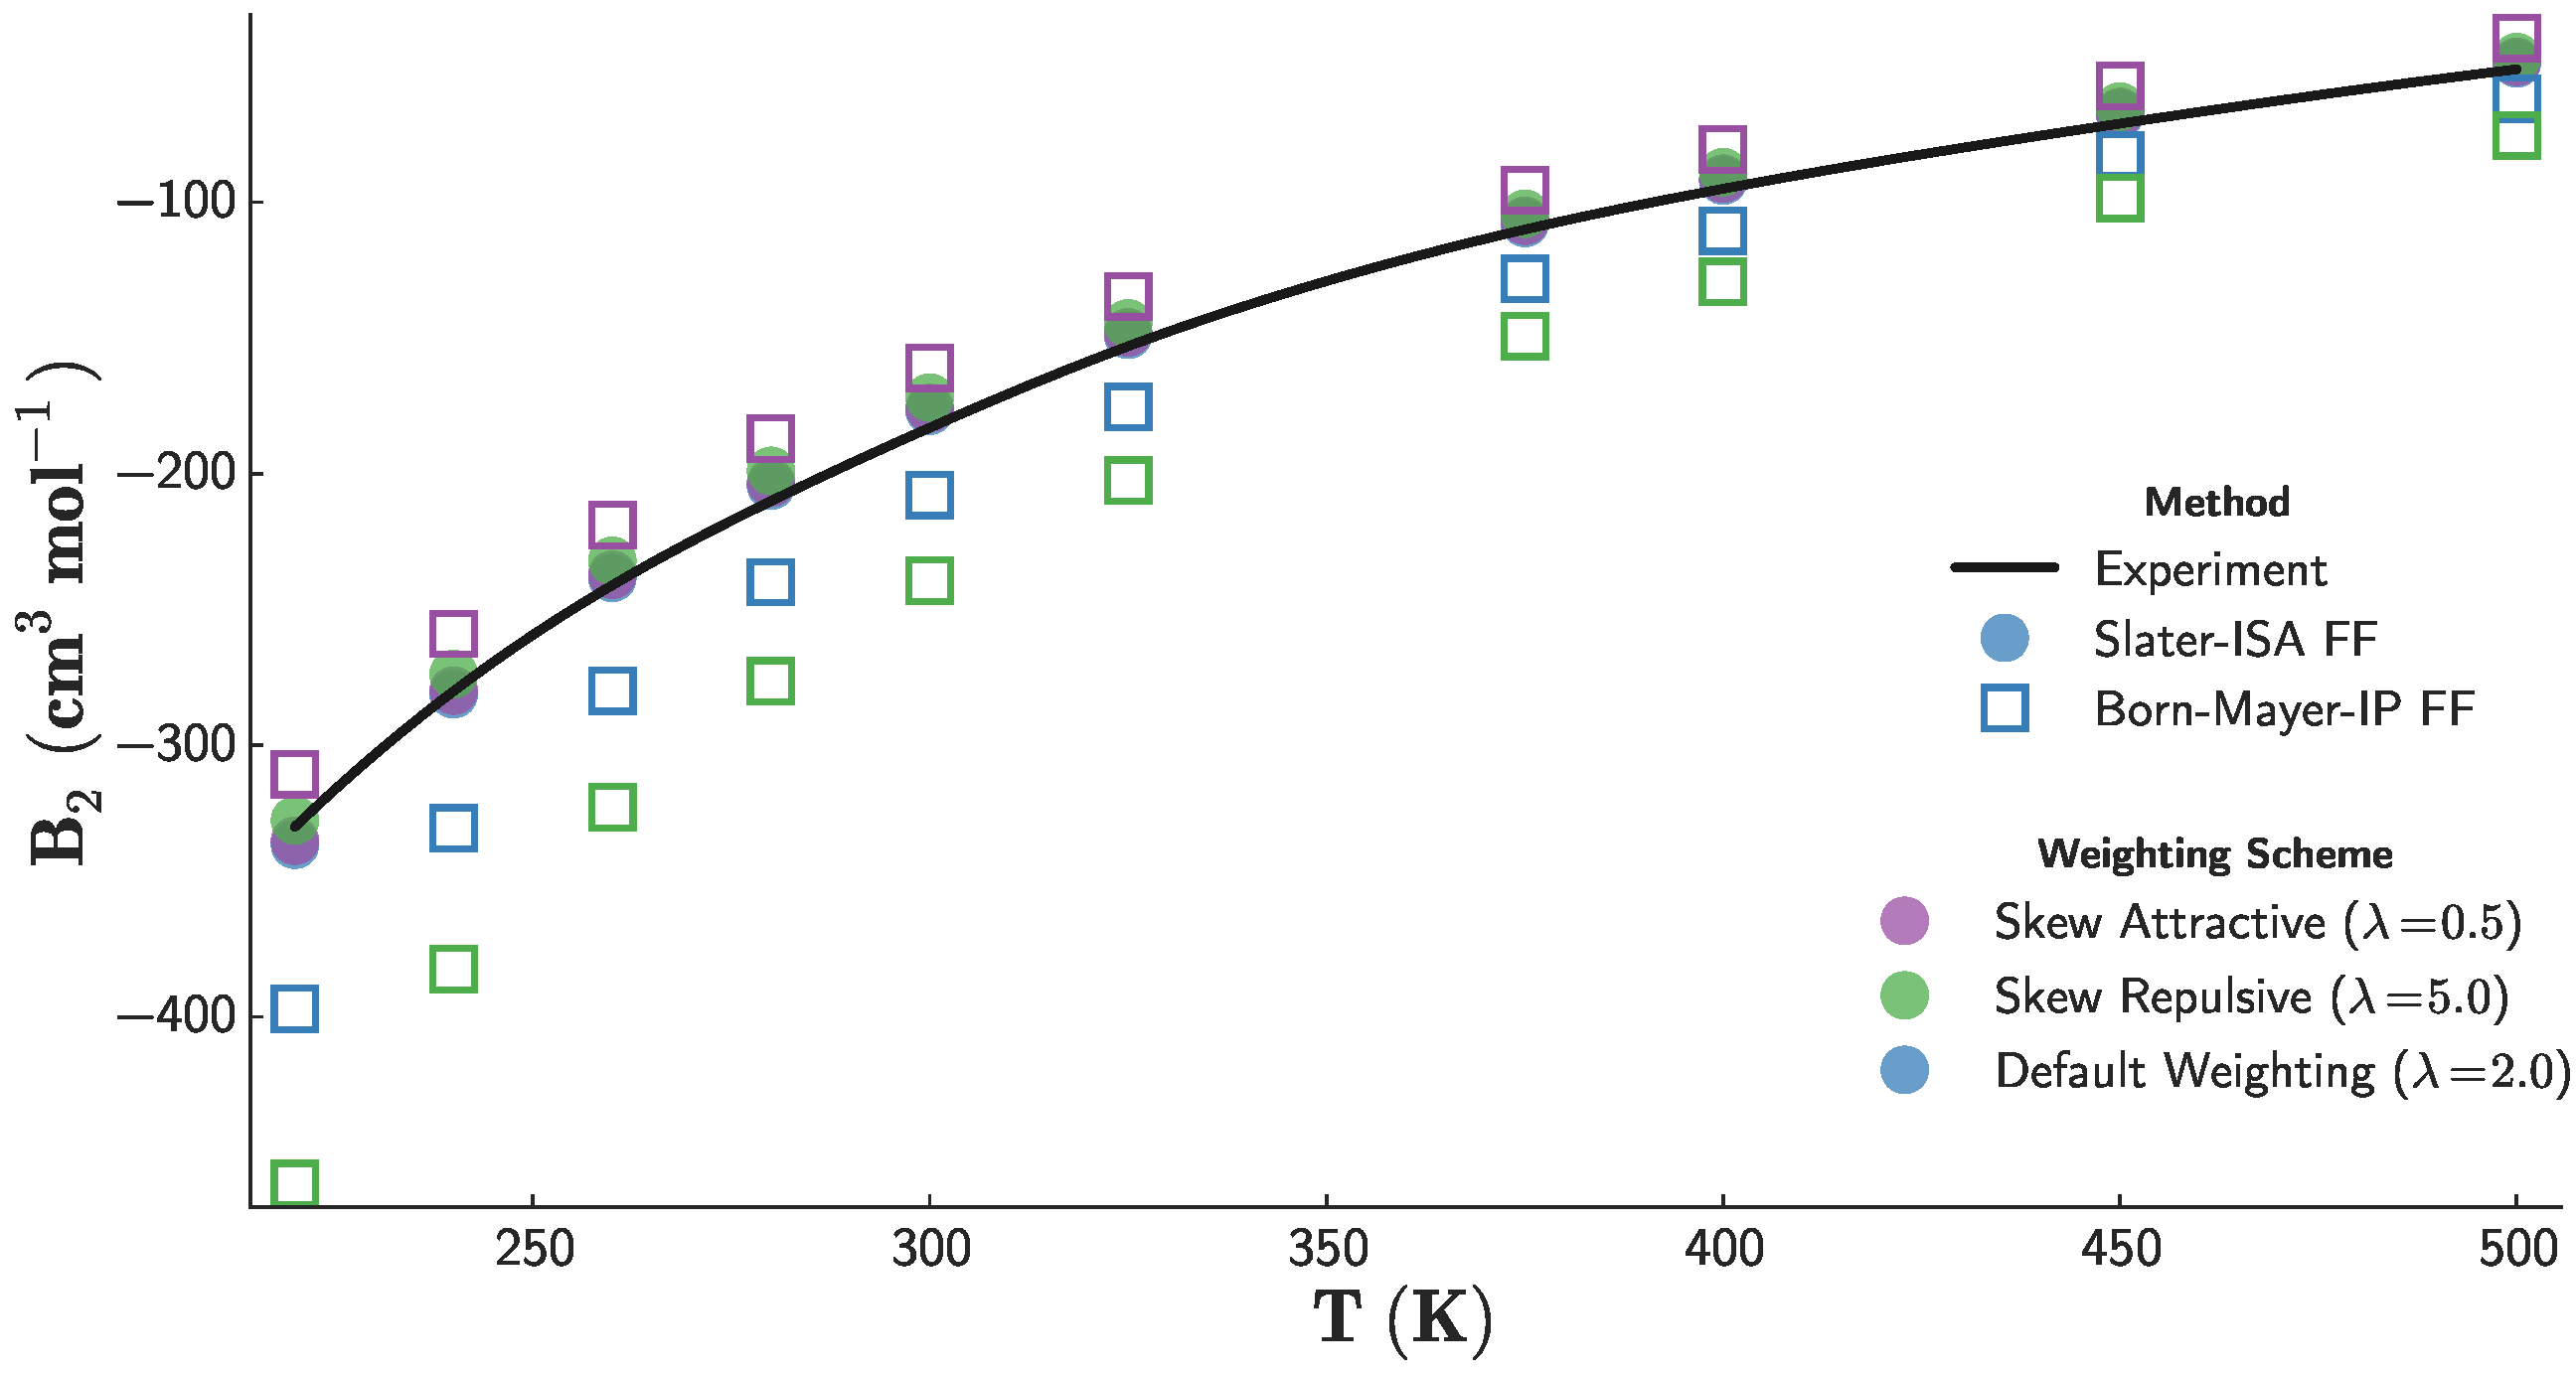
\includegraphics[width=0.9\textwidth]{isotropic/weighted_ethane_2nd_virial.pdf}
      \caption[foo]{
        Comparison of the \isaffold and the \saptff in terms of sensitivity to the
        weighting function employed in parameter optimization for the ethane
        dimer. Three weighting functions, $\lambda = 0.5$ (purple), $\lambda = 2.0$
        (blue), and $\lambda = 5.0$ (green) are shown, with higher $\lambda$ values
        indicating more weighting of repulsive configurations.
        
        (top) Total interaction energies for the \isaffold (left) and the \saptff (right)
        indicating the accuracy of each force field with respect to \saptpbeo benchmark
        energies.  The diagonal line (black) indicates perfect agreement between
        reference energies and each force field, while shaded grey areas represent
        points within $\pm 10\%$ agreement of the benchmark.  To guide the eye, a line
        of best fit (dotted line) has been computed for each force field and for each
        weighting function.
        
        (bottom) Computed 2$^\text{nd}$ virial coefficients for ethane. Data for
        the \isaffold and the \saptff are depicted using shaded circles and open squares,
        respectively; colors for the different weighting functions are as above.
        Experimental data from \citen{Dymond1980} (black line) is also shown.
        %ASK: Do we actually cite Dymond and Smith for this, since it's a compiled
        %work, or do I need to try and dig up the original experimentalist?
    }
    \label{fig:isotropic-ethane-weighting}

    \end{figure}
    %%%%%%%% Weighting Function Tests %%%%%%%

The \isaffold fits for the ethane dimer, on the other hand, are nearly completely
insensitive to the weighting function, leading to little intrinsic uncertainty
in the determination of parameters or in the computation of macroscopic
properties. Some other dimers, particularly those where
atomic anisotropy would be anticipated (e.g., water), exhibited slightly larger
sensitivity to the weighting function. Nevertheless, the
vast majority of dimers in the test set are qualitatively insensitive to the choice of
weighting function, and can be optimized with the default $\lambda = 2.0$
weighting function without yielding undue systematic error in the attractive
region of the potential, thus proving the enhanced robustness of the \isaffold
model relative to conventional force fields.

\end{subsection}
\begin{subsection}{Next-Generation Born-Mayer Models: \bmsisaff}

We hypothesize that the increased accuracy, transferability, and robustness of
the \isaffold is a direct result of its more physically-motivated functional form and
its use of ISA-derived atomic exponents that directly account for the influence
of the molecular environment. Nonetheless, we recognize that the standard
Born-Mayer functional form remains extremely common, both in simulation software and in
existing force fields. It is therefore fruitful to explore the extent to which the \bsisa
exponents themselves could be used in conjunction with a Born-Mayer functional
form. These results are shown in \cref{tab:isotropic-bmsisaff_rmse}.

%%%%%%%%%%%%%%%%%%%%% Average RMSE Table %%%%%%%%%%%%%%%%%%%%%%%%%%%%%%%%%%%
\begin{landscape}
\begin{table}
\footnotesize
\centering
\renewcommand\arraystretch{1.1}
\begin{tabular}{@{}rcccccccc@{}}
\hline
\toprule
& \phantom{ab} &
  \multicolumn{3}{c}{Dimer-Specific Fits} &
  \phantom{ab} &
  \multicolumn{3}{c}{Transferable Fits} \\
\cmidrule{3-5} \cmidrule{7-9}

Component & & \isaffold & Born-Mayer-ISA & Born-Mayer-sISA & & \isaffold & Born-Mayer-ISA & Born-Mayer-sISA  \\
     & & \multicolumn{1}{c}{(kJ mol$^{-1}$)} & \multicolumn{1}{c}{(kJ mol$^{-1}$)} &  \multicolumn{1}{c}{(kJ mol$^{-1}$)}
     & & \multicolumn{1}{c}{(kJ mol$^{-1}$)}& \multicolumn{1}{c}{(kJ mol$^{-1}$)} &  \multicolumn{1}{c}{(kJ mol$^{-1}$)} \\
\midrule
Exchange        & &    2.641 (0.686)   &  7.030 (1.203)     &  2.677 (0.686)  & &    2.718 (0.720)  &  6.968 (1.228)  & 2.764 (0.706) \\
Electrostatics  & &    1.087 (0.351)   &  1.406 (0.589)     &  1.083 (0.352)  & &    1.134 (0.351)  &  1.461 (0.598)  & 1.141 (0.352) \\
Induction       & &    0.251 (0.095)   &  0.229 (0.097)     &  0.250 (0.096)  & &    0.278 (0.101)  &  0.257 (0.101)  & 0.275 (0.101) \\
\dhf            & &    0.246 (0.068)   &  0.327 (0.120)     &  0.248 (0.068)  & &    0.274 (0.076)  &  0.353 (0.122)  & 0.274 (0.076) \\
Dispersion      & &    0.766 (0.317)   &  3.584 (0.890)     &  0.856 (0.336)  & &    0.766 (0.317)  &  3.584 (0.890)  & 0.856 (0.336) \\
\addlinespace                                                                                                           
\textbf{                                                                                                                    
Total Energy}   \\
\emph{RMSE}
                & &    1.701 (0.464)   &  4.934 (1.054)     &  1.751 (0.453)  & &    1.650 (0.456)  &  4.555 (1.035)  & 1.713 (0.446) \\
\emph{\mse}
                & &    0.216 (0.057)   &  1.127 (0.505)     &  0.258 (0.063)  & &    0.175 (0.051)  &  0.882 (0.516)  & 0.245 (0.057) \\
\bottomrule

\hline
\end{tabular}
\caption{
    Comparison of characteristic RMSE (as described in the main text) over the 91 dimer test
set for the 
    Born-Mayer-sISA approximation compared with other methods.
    For the total energy, both RMSE and absolute mean signed errors
    (MSE) have been shown.
    `Attractive' RMSE, representing the characteristic RMSE for
    the subset of points whose energies are net attractive ($\etot <
    0$), are shown in parentheses to the right of the total RMS
    errors; `attractive' \mse are likewise displayed for the total
    energy.
    \isaffold, Born-Mayer-ISA, and \bmsisaff are as described in the main text,
and the `Dimer-Specific' and `Transferable' fits are as described in
\cref{tab:isotropic-rmse}.
	}
\label{tab:isotropic-bmsisaff_rmse}
\end{table}
\normalsize
\end{landscape}
%%%%%%%%%%%%%%%%%%%%% Average RMSE Table %%%%%%%%%%%%%%%%%%%%%%%%%%%%%%%%%%%

As expected, direct insertion of the \bsisa exponents into the
Born-Mayer functional form (Born-Mayer-ISA) does not yield promising results.
Indeed, the Born-Mayer-ISA FF has significantly worse RMSE and \mse than
the \saptff. 
We reiterate that the $P = 1$ approximation from \cref{eq:isotropic-isaff_sr}, yielding the
conventional Born-Mayer form, is by itself a crude model.
Rather, it becomes necessary to accompany this approximation by a
corresponding exponent scale factor, $\xi$:
%
\begin{align}
\label{eq:isotropic-bmsisaff_bi}
B_i &= \xi \Bisa{i}.
\end{align}
%
Following literature precedent, 
\cite{Ihm1990, McDaniel2012}
we hypothesized that $\xi$ could be treated as a
universal constant. To test this conjecture, we computed reference density overlaps for a
variety of isolated atom pairs (details in the Supporting Information of
\citen{VanVleet2016}), and
fitted each of these overlaps to a Born-Mayer function of the form 
$S_{ij} \approx K_{ij}\exp(-\xi \Bisa{ij} \R)$, where $K_{ij} =
\frac{K}{B^{3}_{ij}}$ in line with \cref{eq:isotropic-isaff_aij}. To very good
approximation, both $K$ and $\xi$ can be treated as universal constants;
that is, neither $K$ nor $\xi$ is sensitive to the value of $\Bisa{}$.
However, fitted values of $K$ and $\xi$ do depend strongly on the range of \R values
used in the optimization, yielding estimates ranging from 0.74 to 0.88.

As an alternative, we optimized $\xi$ directly by minimizing RMSE
against the 91 dimer test set. Results from various choices
of $\xi$ can be found in the Supporting Information of \citen{VanVleet2016}.  In agreement
with prior literature and our `first-principles' analysis of overlaps, we find $\xi
= 0.84$ to be optimal for minimizing characteristic overall and attractive RMSE,
though in practice the errors are insensitive to $\xi \in [0.82,0.86]$.
We henceforth use $\xi=0.84$ and refer to to this force field methodology
(Born-Mayer functional form, ISA-derived exponents with
scale factor $\xi=0.84$) as the \bmsisaff. 
Parameters and homo-monomeric fits for the \bmsisaff
can be found in the Supporting Information of \citen{VanVleet2016} and in
\cref{sec:isotropic-homomonomeric_fits}.
 
From \cref{tab:isotropic-bmsisaff_rmse} we see that the \bmsisaff is comparable in
quality to our original \isaffold methodology. 
For all attractive configurations, the \bmsisaff is equally
accurate and transferable (\cref{tab:isotropic-bmsisaff_rmse}). Furthermore, as shown in
\cref{tab:isotropic-rmsd-weightings}, \bmsisaff displays similar parameter robustness
to \isaffold. These results suggest that many of the advantages of the \isaffold
procedure can be captured simply by using the (scaled) ISA exponents.
Note, however, that the optimal scale factor likely exhibits some system dependence,
and furthermore that the enhanced Slater functional form may be important
where an accurate description of highly repulsive configurations is crucial.

We also examined the \isaffold and the \bmsisaff against force
fields where $B_i$ values were instead treated as soft constraints, rather than fixed parameters.
Using entirely unconstrained exponents yields unphysical parameters and a 
severe degradation in force field transferability. Using exponents from the \isaffold and
the \bmsisaff as Bayesian priors (in the sense used in
\citens{Misquitta2015a,Misquitta2015b}), 
we generated two new force fields with optimized exponents, denoted Slater-OPT and Born-Mayer-OPT,
respectively. Characteristic RMSE and \mse for these force fields can be found
in the Supporting Information of \citen{VanVleet2016}.
We find that both methods yield only very minimal improvement, suggesting that the
first-principles ISA exponents are already nearly optimal. Comparing the Born-Mayer-OPT
exponents to those from Slater-ISA, we find a nearly identical average scale factor
of $\gamma = 0.83 \pm 0.07$.  Given that these optimal exponents can now be generated
directly from first principles calculations of the molecular densities via the \bsisa 
approach of \citeauthor{Misquitta2014}, we anticipate that the \bsisa densities and
resulting ISA exponents will be extremely useful in next-generation force field
development in order to greatly simplify force field parameterization.

\end{subsection}


\end{section}
%%%%%%%%%%%%%%%%%%%%%%%%%%%%%%%%%% Results %%%%%%%%%%%%%%%%%%%%%%%%%%%%%%%%%%%%%%%%





%%%%%%%%%%%%%%%%%%%%%%%%%%%%% Conclusions %%%%%%%%%%%%%%%%%%%%%%%%%%%%%%%%%%%%%%%%%
\begin{section}{Conclusions and Recommendations}
\label{sec:isotropic-conclusions}

%auto-ignore
We have presented a new methodology for describing short-range intermolecular
interactions based upon a simple model of atom-in-molecule electron density
overlap. The resulting \isaffold is a simple extension of the conventional
Born-Mayer functional form, supplemented with atomic exponents determined from
an ISA analysis of the molecular electron density. 
In contrast to simple Born-Mayer or Lennard-Jones models, the \isaffold is capable of
reproducing ab initio interaction energies over a wide range of inter-atomic
distances, and displays
extremely low sensitivity to the details of parameterization. Furthermore, the
\isaffold exhibits excellent parameter transferability. We thus recommend
\isaffold for use in the development of future ab initio (and possibly
empirically-parameterized) potentials, particularly where accuracy across wide
regions of the potential surface is paramount. 

More generally, we find that analysis of the ISA densities provides an
excellent first-principles procedure for the determination of atomic-density
decay exponents.  This analysis improves upon existing approaches (which rely
upon exponents derived from atomic radii or ionization
potentials)\cite{Rappe1992, Mayo1990, Lim2009, VanDuin2001} and explicitly
incorporates the influence of the molecular environment.  These exponents can
be used within \isaffold without further parameterization.  Alternatively, in
conjunction with an appropriate scale factor, the exponents can be used to
enhance the accuracy of standard Born-Mayer potentials and/or Tang-Toennies
damping functions. The resulting \bmsisaff retains many of the advantages of
\isaffold, but also maintains compatibility with existing force fields and
simulations packages that do not support the Slater functional form.  
Given that the \bsisa exponents appear to be essentially
optimal with respect to additional empirical optimization, we strongly
recommend use of these first-principles exponents in order to simplify 
(both ab initio and empirical) future force field development involving Born-Mayer
or related functional forms.\cite{Gordon2006}

Overall, \isaffold enables a significantly increase in force field accuracy,
particularly in describing short intermolecular contacts. Nevertheless, the
neglect of atomic anisotropy remains, in some cases, a severe approximation.
\cite{Eramian2013, Badenhoop1997, Kim2014b}
Indeed, it has been shown by many
authors\cite{stone2013theory,Day2003,Totton2010a,Wheatley1990} that
quantitatively accurate \A parameters (and to a lesser extent, \B parameters)
require incorporation of angular dependence for the generation of
highly-accurate force fields. This anisotropy becomes crucial when describing
systems containing lone pairs, hydrogen bonds, and/or $\pi$-interactions.
Promisingly, \bsisa densities naturally describe such anisotropy, 
\cite{Wheatley2012,Misquitta2015a,Misquitta2015b}
and a straightforward method for its inclusion (where essential) in
ab initio force fields is the subject of \cref{ch:mastiff}.


\end{section}
%%%%%%%%%%%%%%%%%%%%%%%%%%%%% Conclusions %%%%%%%%%%%%%%%%%%%%%%%%%%%%%%%%%%%%%%%%%

\begin{subappendices}
%% \documentclass[12pt,letterpaper]{article}
%% \usepackage[margin=1in,bottom=1in]{geometry} % see geometry.pdf on how to lay out the page. There's lots.
%% 
%% \usepackage{hyperref}
%% \usepackage[journal=jacs]{chemstyle} %Other chemical formatting
%% \usepackage{chemscheme} % Chemical graphics
%% \usepackage{chemcompounds}
%% \usepackage{caption}
%% \usepackage{bpchem} % Chemical compounds
%% \usepackage{setspace}
%% \usepackage{fullpage}
%% \usepackage{graphicx}
%% \usepackage{xspace}
%% \usepackage{booktabs}
%% \usepackage{pdflscape}
%% \usepackage[sort&compress,numbers,super]{natbib}
%% \usepackage{bibentry}
%% %\usepackage{xr}
%% %\externaldocument{isa_ff}
%% \usepackage{amsmath}
%% \usepackage{longtable}
%% \usepackage{xfrac}
%% \usepackage{multirow}
%% \usepackage{dcolumn}
%% \usepackage{siunitx}
%% \usepackage{subcaption}
%% 
%% %eqref
%% \usepackage{letltxmacro}
%% \LetLtxMacro{\originaleqref}{\eqref}
%% \renewcommand{\eqref}{eq.~\originaleqref}
%% \newcommand{\Eqref}{Eq.~\originaleqref}
%% 
%% %figref
%% \newcommand{\figref}[1]{Figure~\ref{#1}}
%% \newcommand{\tabref}[1]{Table~\ref{#1}}
%% \newcommand{\secref}[1]{Section~\ref{#1}}
%% 
%% \newcommand{\super}[1]{\textsuperscript{#1}}
%% \newcommand{\sub}[1]{\textsubscript{#1}}
%% \renewcommand{\thefootnote}{\fnsymbol{footnote}}
%% \newcommand{\ra}[1]{\renewcommand{\arraystretch{#1}}}
%% \newcommand{\centercell}[1]{\multicolumn{1}{C}{#1}}
%% 
%% % Supplementary Information Labels
%% \newcommand{\beginsupplement}{%
%%         \setcounter{table}{0}
%%         \renewcommand{\thetable}{S\arabic{table}}%
%%         \setcounter{figure}{0}
%%         \renewcommand{\thefigure}{S\arabic{figure}}%
%%         \setcounter{section}{0}
%%         \renewcommand{\thesection}{S\arabic{section}}%
%%      }
%% 
%% \newcommand*{\citen}[1]{%
%%   \begingroup
%%     \romannumeral-`\x % remove space at the beginning of \setcitestyle
%%     \setcitestyle{numbers}%
%%     ref. \cite{#1}%
%%   \endgroup   
%% }
%% 
% ISA-FF Paper lingo
%% \newcommand{\isa}{BS-ISA\xspace}
%% \newcommand{\isaffold}{Slater-ISA FF\xspace}
%% \newcommand{\saptff}{Born-Mayer-IP FF\xspace}
%% \newcommand{\bmsisaff}{Born-Mayer-sISA FF\xspace}
%% \newcommand{\saptpbeo}{DFT-SAPT (PBE0/AC)\xspace}
%% \newcommand{\avtz}{aug-cc-pVTZ\xspace}
%% \newcommand{\A}{\ensuremath{A_{ij}}\xspace}
%% \newcommand{\B}{\ensuremath{B_{ij}}\xspace}
%% \newcommand{\C}{\ensuremath{C_{ij,n}}\xspace}
%% \newcommand{\R}{\ensuremath{r_{ij}}\xspace}
%% 
%% \newcommand{\dhf}{\ensuremath{\delta^{\text{HF}}}\xspace}
%% 
%% \newcommand{\vtot}{\ensuremath{V_{FF}}\xspace}
%% \newcommand{\vrep}{\ensuremath{V^{exch}}\xspace}
%% \newcommand{\vcp}{\ensuremath{V^{pen}}\xspace}
%% \newcommand{\vsrind}{\ensuremath{V^{ind,sr}}\xspace}
%% \newcommand{\vsrdisp}{\ensuremath{V^{disp,sr}}\xspace}
%% \newcommand{\velst}{\ensuremath{V^{elst}}\xspace}
%% \newcommand{\vind}{\ensuremath{V^{ind}}\xspace}
%% \newcommand{\vdhf}{\ensuremath{V^{\dhf}}\xspace}
%% \newcommand{\vdisp}{\ensuremath{V^{disp}}\xspace}
%% \newcommand{\vlr}{\ensuremath{V_{lr}}\xspace}
%% \newcommand{\vmultipole}{\ensuremath{\sum\limits_{tu}Q_t^iT_{tu}Q_u^j}\xspace}
%% \newcommand{\vdrude}{\ensuremath{V_{shell}}\xspace}
%% \newcommand{\vdrudeind}{\ensuremath{V_{shell}^{(2)}}\xspace}
%% \newcommand{\vdrudescf}{\ensuremath{V_{shell}^{(3-\infty)}}\xspace}
%% 
\newcommand{\sijapprox}{\ensuremath{S^{ij}_{B_i = B_j}}\xspace}
\newcommand{\sijexact}{\ensuremath{S^{ij}_{B_i \ne B_j}}\xspace}
%% 
%% % ISA-FF Paper lingo
%% \newcommand{\isa}{BS-ISA\xspace}
%% \newcommand{\isaffold}{Slater-ISA FF\xspace}
%% \newcommand{\saptff}{Born-Mayer-IP FF\xspace}
%% \newcommand{\bmsisaff}{Born-Mayer-sISA FF\xspace}
%% \newcommand{\ljff}{LJ FF\xspace}
%% \newcommand{\saptpbeo}{DFT-SAPT (PBE0/AC)\xspace}
%% \newcommand{\avtz}{aug-cc-pVTZ\xspace}
%% \newcommand{\A}{\ensuremath{A_{ij}}\xspace}
%% \newcommand{\B}{\ensuremath{B_{ij}}\xspace}
%% \newcommand{\C}{\ensuremath{C_{ij,n}}\xspace}
%% \newcommand{\R}{\ensuremath{r_{ij}}\xspace}
%% 
%% \newcommand{\dhf}{\ensuremath{\delta^{\text{HF}}}\xspace}
%% 
%% \newcommand{\Asr}[1]{\ensuremath{A^{\text{sr}}_{#1}}\xspace}
%% \newcommand{\Aex}[1]{\ensuremath{A^{\text{exch}}_{#1}}\xspace}
%% \newcommand{\Ael}[1]{\ensuremath{A^{\text{elst}}_{#1}}\xspace}
%% \newcommand{\Apen}[1]{\ensuremath{A^{\text{pen}}_{#1}}\xspace}
%% \newcommand{\Aind}[1]{\ensuremath{A^{\text{ind}}_{#1}}\xspace} % AJM Not ind,sr !!!
%% \newcommand{\Adhf}[1]{\ensuremath{A^{\dhf}_{#1}}\xspace} % AJM Not ind,sr !!!
%% 
%% \newcommand{\Bisa}[1]{\ensuremath{B^{\text{ISA}}_{#1}}\xspace}
%% \newcommand{\Bip}[1]{\ensuremath{B^{\text{IP}}_{#1}}\xspace}
%% 
%% \newcommand{\etot}{\ensuremath{E_{\text{int}}}\xspace}
%% \newcommand{\erep}{\ensuremath{E^{\text{exch}}}\xspace}
%% \newcommand{\eelst}{\ensuremath{E^{\text{elst}}}\xspace}
%% \newcommand{\eind}{\ensuremath{E^{\text{ind}}}\xspace}
%% \newcommand{\edhf}{\ensuremath{E^{\dhf}}\xspace}
%% \newcommand{\edisp}{\ensuremath{E^{\text{disp}}}\xspace}
%% 
%% \newcommand{\vtot}{\ensuremath{V_{\text{FF}}}\xspace}
%% \newcommand{\vrep}{\ensuremath{V^{\text{exch}}}\xspace}
%% \newcommand{\vcp}{\ensuremath{V^{\text{pen}}}\xspace}
%% \newcommand{\vsrind}{\ensuremath{V^{\text{ind,sr}}}\xspace}
%% \newcommand{\vsrdisp}{\ensuremath{V^{\text{disp,sr}}}\xspace}
%% \newcommand{\velst}{\ensuremath{V^{\text{elst}}}\xspace}
%% \newcommand{\vind}{\ensuremath{V^{\text{ind}}}\xspace}
%% \newcommand{\vdhf}{\ensuremath{V^{\dhf}}\xspace}
%% \newcommand{\vdisp}{\ensuremath{V^{\text{disp}}}\xspace}
%% \newcommand{\vlr}{\ensuremath{V_{lr}}\xspace}
%% \newcommand{\vmultipole}{\ensuremath{\sum\limits_{tu}Q_t^iT_{tu}Q_u^j}\xspace}
%% \newcommand{\vdrude}{\ensuremath{V_{\text{shell}}}\xspace}
%% \newcommand{\vdrudeind}{\ensuremath{V_{\text{shell}}^{(2)}}\xspace}
%% \newcommand{\vdrudescf}{\ensuremath{V_{\text{shell}}^{(3-\infty)}}\xspace}
%% 
%% \newcommand{\mse}{\ensuremath{\lVert\text{MSE}\rVert}\xspace}
%% 
%% \title{\textbf{Supporting Information} \\ for \\
%% `Beyond Born-Mayer: Improved models for short-range repulsion in ab initio
%% force fields'
%% }
%% \author{Mary J. Van Vleet, Alston J. Misquitta, Athony J. Stone, J.R. Schmidt}
%% %\date{April 23, 2015} % delete this line to display the current date
%% 
%% \begin{document}
%% \beginsupplement
%% \maketitle
%% \tableofcontents
%% 
%% 
%% %%%%%%%%%%%%%%%%%%%%%%%%%%%%%%%%% SI %%%%%%%%%%%%%%%%%%%%%%%%%%%%%%%%%%%%%%%%%%%%%%
%% \onehalfspacing
%% 
\begin{section}{Waldman-Hagler Analysis of $B_{ij}$ Combination Rule}
\label{sec:bij_combo_rule}

The exact expressions for the overlap of two Slater densities 
$\rho_i = D_i \exp(-B_i r)$ and $\rho_j = D_j \exp(-B_j r)$ 
are shown here, first in the limiting case where the two
exponents are equal ($B_i = B_j = B_{ij}$): 

\begin{align}
\label{eq:simple_overlap}
\begin{split}
%S^{ij}_{b_i = b_j} &= D_{ij} P(B_{ij}, r_{ij}) \exp(-B_{ij}r_{ij}) \\
\sijapprox &= D_{ij} P(B_{ij}, r_{ij}) \exp(-B_{ij}r_{ij}) \\
D_{ij} &= \pi D_i D_j B_{ij}^{-3} \\
P(B_{ij},r_{ij}) &= \frac13 (B_{ij} r_{ij})^2 + B_{ij} r_{ij} + 1 ,
\end{split}
\end{align}

and second in the case where $B_i \ne B_j$:

\begin{align}
\label{eq:complicated_overlap}
\begin{split}
%S^{ij}_{b_i\ne b_j} = &
\sijexact = &
\frac{16\pi D_i D_j \exp(-\{B_i + B_j\}r_{ij}/2)}{(B_i^2-B_j^2)^3r_{ij}}
\times \\
\Bigg [ &
\left(\frac{B_i - B_j}{2}\right)^2 
\bigg(\exp \left(\{B_i-B_j\}\frac{r_{ij}}{2}\right) - \exp \left(-\{B_i-B_j\}\frac{r_{ij}}{2}\right) \bigg) \\
& \qquad \times \left( \left(\frac{B_i + B_j}{2}\right)^2r_{ij}^2 + (B_i + B_j)r_{ij} + 2 \right) \\
& - \left(\frac{B_i + B_j}{2}\right)^2 \exp \left(\{B_i-B_j\}\frac{r_{ij}}{2}\right)
\times \left( \left(\frac{B_i - B_j}{2}\right)^2r_{ij}^2 - (B_i - B_j)r_{ij} + 2 \right) \\
& + \left(\frac{B_i + B_j}{2}\right)^2 \exp \left(-\{B_i-B_j\}\frac{r_{ij}}{2}\right)
\times \left( \left(\frac{B_i - B_j}{2}\right)^2r_{ij}^2 + (B_i - B_j)r_{ij} + 2 \right)
\Bigg ] .
\end{split}
\end{align}
Each overlap formula has been given a subscript to indicate
limits on $B_i$ and $B_j$.

Our goal is to ascertain the extent to which \sijexact can
be accurately modeled by the functional form and variables of \sijapprox.
$D_i$ and $D_j$ are pre-factors appearing in both equations, and we set
these variables to unity without loss of generality. To 
find values of \B such that $\sijexact(B_i,B_j,r_{ij}) \approx
\sijapprox(\B,r_{ij})$, we first treat \B as a completely adjustable
parameter, and later test for the existence of some simple combining function
$f$ such that $\B = f(B_i, B_j)$.

To optimize $\B$, we first require a training set of
relevant \sijexact values. $B_i$, $B_j$, and $r_{ij}$ are the only
variables appearing in \sijexact, and we could in principle fit \B values over a
grid of $B_i$, $B_j$ and \R
combinations. However, we are only interested in the subset of 
points which are chemically relevant.
Consequently, we developed a
library of $B_i$ values by deriving exponents from the ionization potentials of the first three rows of
the periodic table (plus bromine and iodine).
For each pair of elements, $B = 2\sqrt{2\text{IP}},$\cite{Yu2011} and a range of \R
values corresponding to 0.8-1.2 times the sum of the van der Waals radii of the two
atoms was selected. \B values in \sijapprox were
then optimized (in a least-squares sense) for each element pair separately;
Mean absolute percent errors (MAPE) for fitted overlaps are shown
in \ref{fig:bij_mape} and in \ref{tab:all_bij_exponents}.


    %%%%%%%%%%%%%%% Bij MAPE %%%%%%%%%%%%%%%%%
    \begin{figure}[t]
    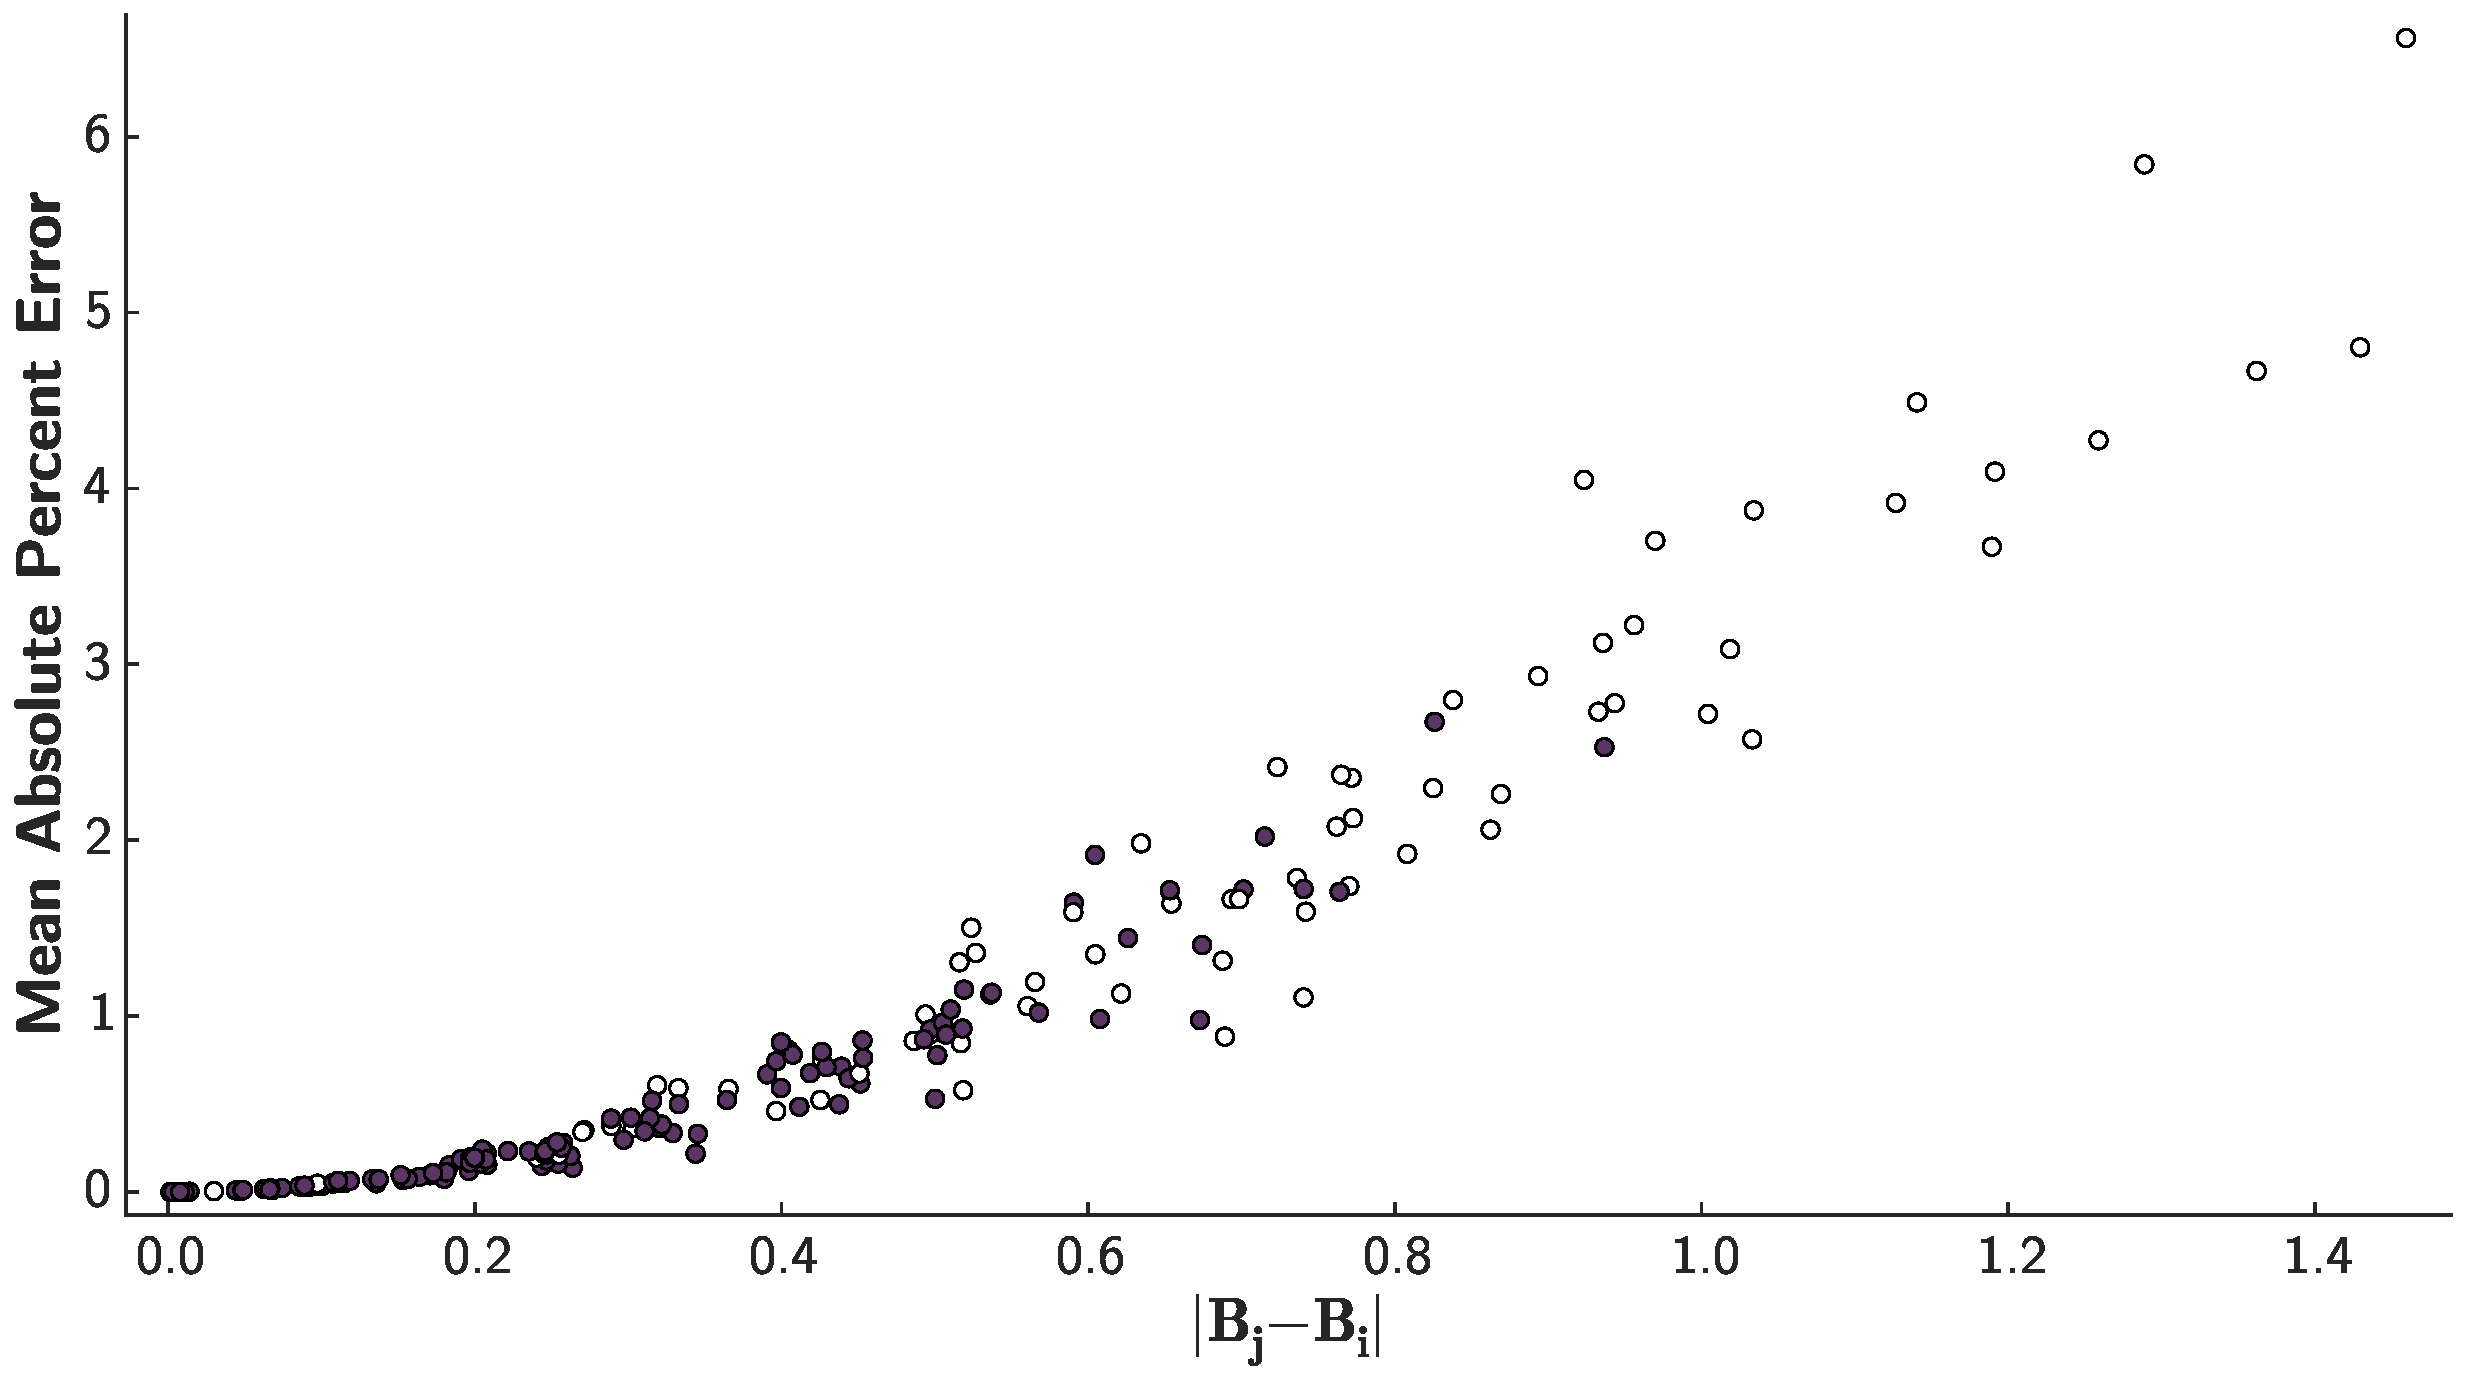
\includegraphics[width=0.9\textwidth]{isotropic/si/bij_mape.pdf}
    \caption{
        Mean absolute percent error of fitted overlap values as a function of the
        absolute difference between $B_i$ and $B_j$ values. Element pairs containing
        He, Li, Ne and/or Na are shown as empty circles.  Deviations below 1\% are
        seen for most element pairs, with noble gases and alkali metals posing a more
        significant challenge. Scatter in the plot is due to small variations in the
        absolute values of \R fit for each pair.  As expected, \sijexact and
        \sijapprox closely agree for $|B_i - B_j| \approx 0$. 
           		  }
    \label{fig:bij_mape}
    \end{figure}
    %%%%%%%%%%%%%%% Bij MAPE %%%%%%%%%%%%%%%%%

Relative errors for fitting are acceptably small for all element pairs.
Excluding certain noble gases and alkali metals (He, Li, Ne,
Na) from consideration, these being the elements with the most disparate $B_i$
values compared to other elements, MAPE drops below 3\% for all pairs, with
the vast majority of MAPE below 1\%. Our focus in this work is primarily on
organic compounds where $|B_i - B_j|$ is small; empirically, these errors always translate to very small
errors in the exchange energy itself.  
Use of an effective \B may require further testing in cases with extremely
disparate $B_i$ and $B_j$ values.

We next tested whether the optimized \B could instead be modeled by
a combination rule $\B = f(B_i,B_j)$.  On the basis of symmetry and scaling
considerations, \citeauthor{Waldman1993} demonstrate that if a
combination rule $f(B_i,B_j)$ exists, a plot of $\sfrac{\B}{B_i}$ vs.
$\sfrac{B_j}{B_i}$ should lie on a single curve.\cite{Waldman1993} Remarkably
(see \ref{fig:bij_combination_rule}), a geometric mean combination rule $\B =
\sqrt{B_iB_j}$ models the fitted \B values near quantitatively. This
result allows the computation of Slater overlaps
using the much simpler
form of \sijapprox (\ref{eq:simple_overlap}) 
from individual atoms-in-molecule exponents $B_i$ and $B_j$.

    %%%%%%%%% Bij Combination Rule %%%%%%%%%%%
    \begin{figure}[t]
    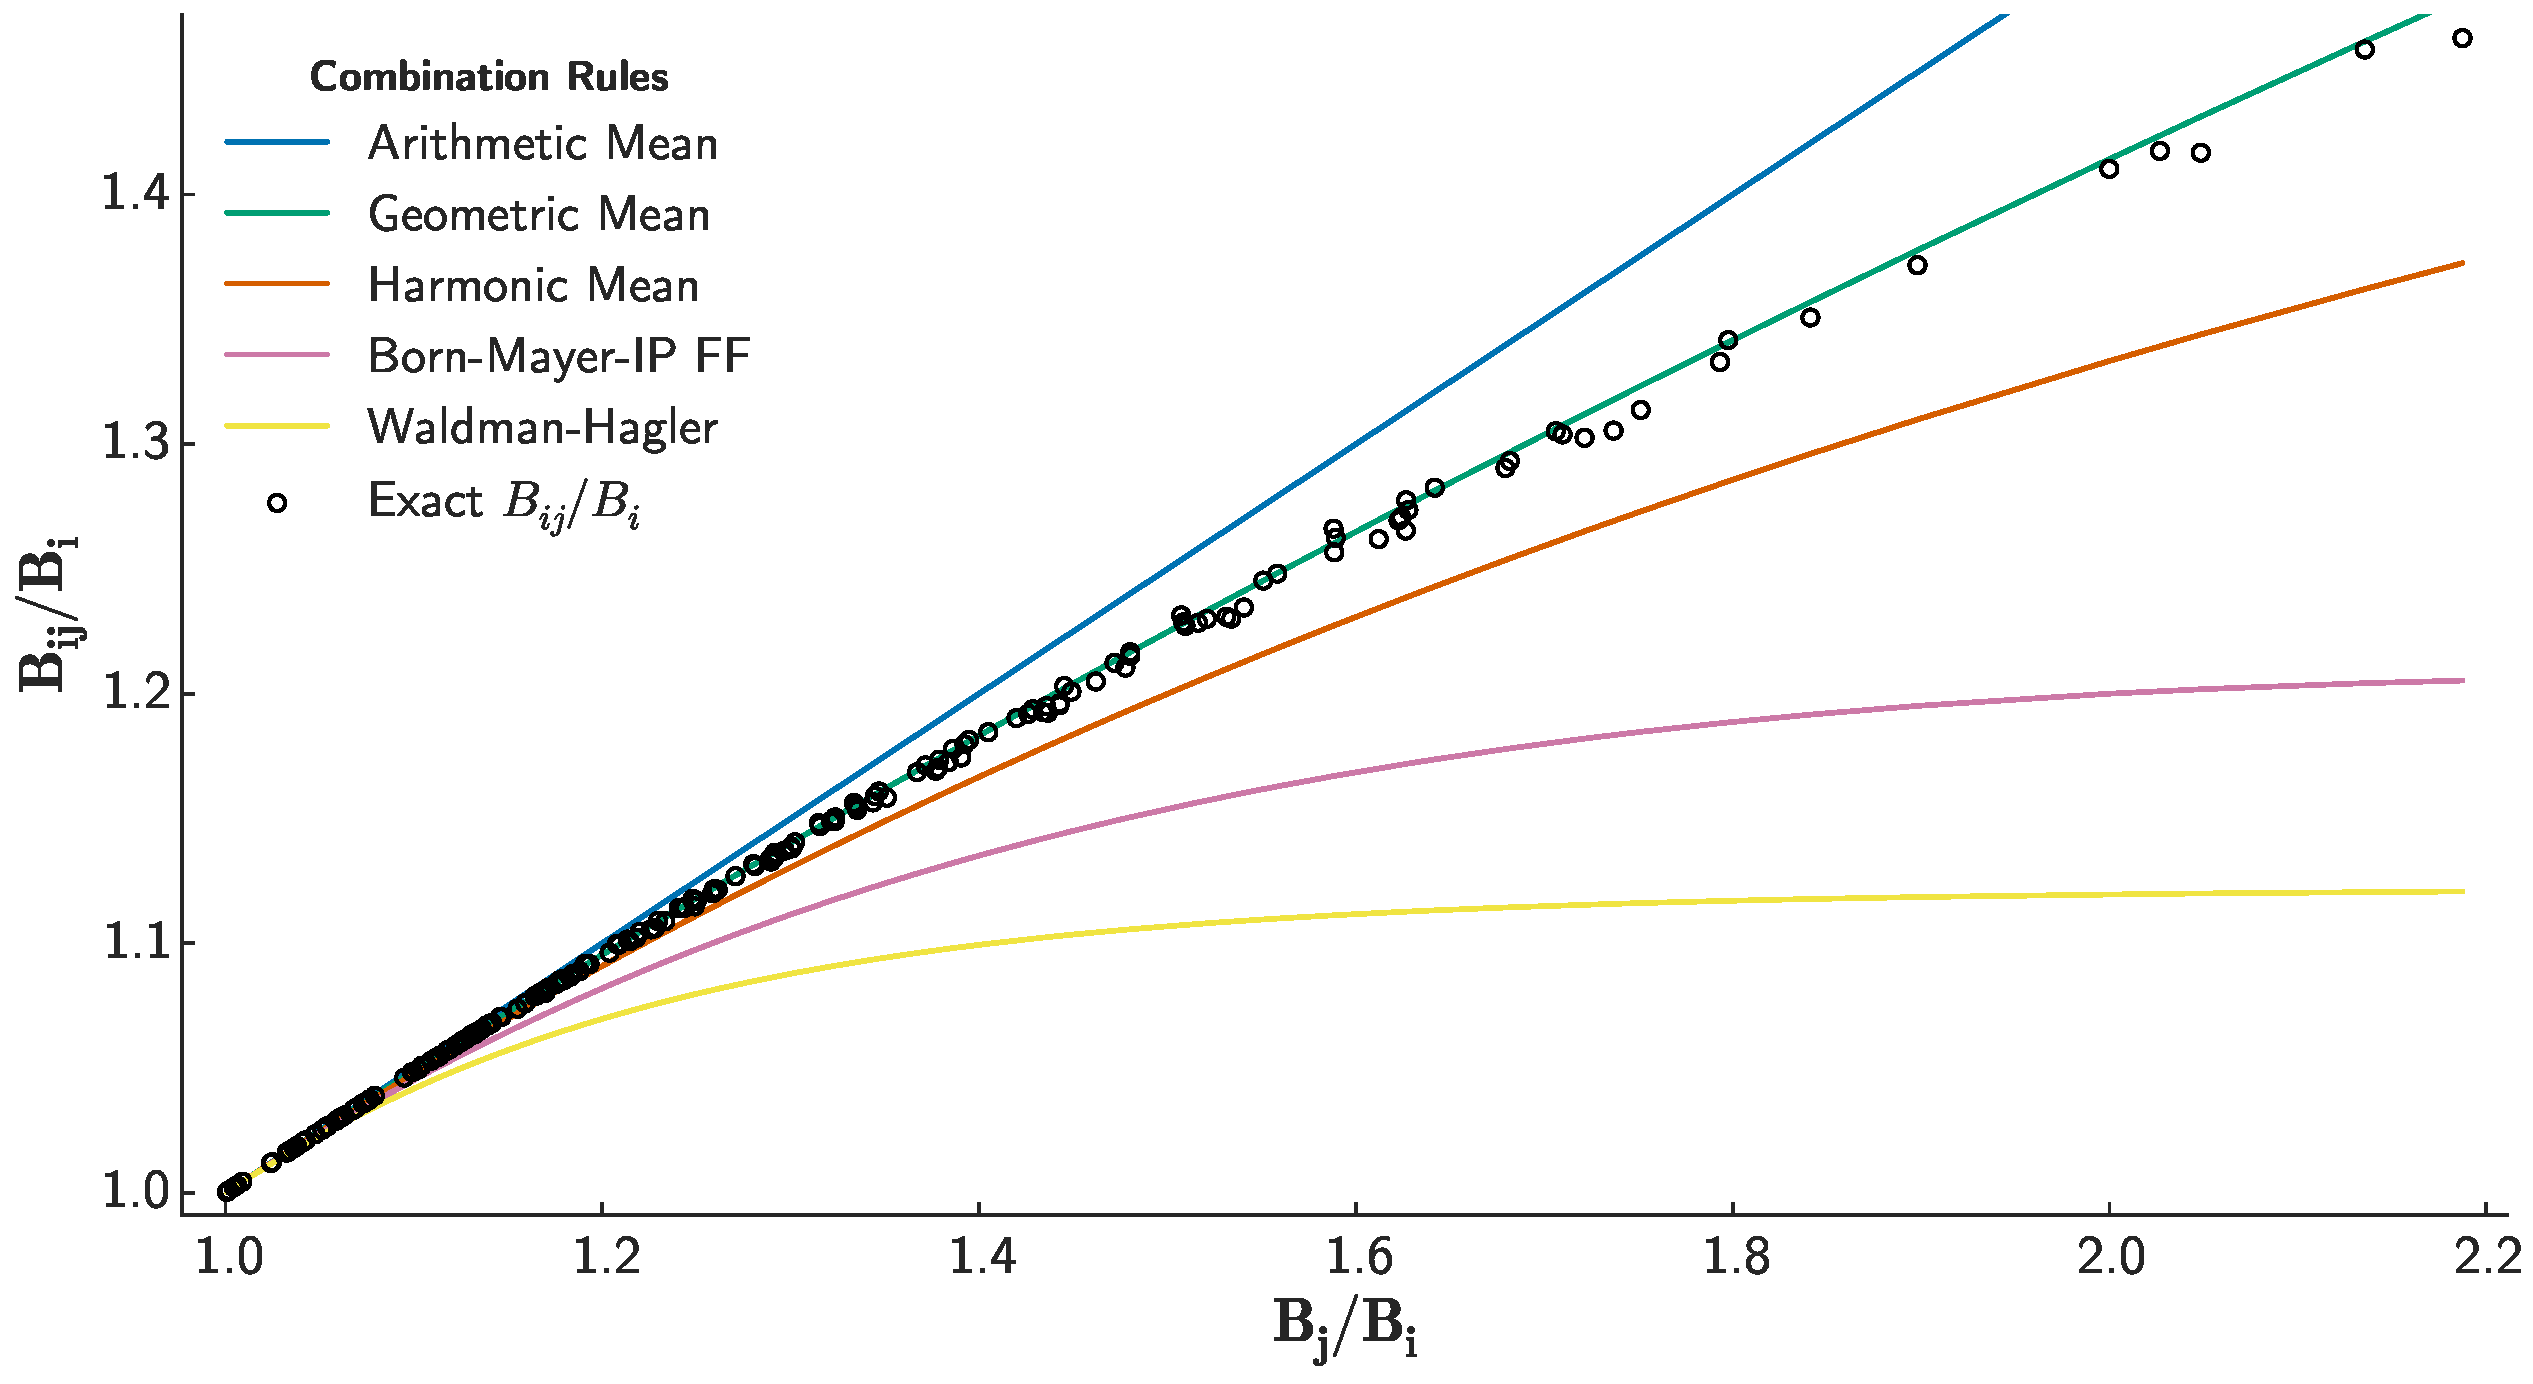
\includegraphics[width=0.9\textwidth]{isotropic/si/bij_combination_rule.pdf}
    \caption{
    Waldman-Hagler-style analsysis of possible $B_{ij}$ combination rules.  Exact
    $B_{ij}$ values are derived from fitting an approximate overlap density of the form $S_{ij}
    = A_{ij} K_2(r_{ij})\exp(-B_{ij}r_{ij})$ to the exact overlap density (as given by Rosen
    and by Tai\cite{Rosen1931,Tai1986}) of two distinct Slater orbitals whose exponents
    correspond to atomic exponents for the elements H-Ar, Cl, Br, and I. For each overlap pair,
    a range of \R values was used from 0.8 to 1.2 times the sum of the pair's van der Waals radii.
    The geometric mean combination rule $B_{ij} = \sqrt{B_iB_j}$ models the exact $B_{ij}$
    values with near-perfect agreement, justifying our choice of combination rule.
           		  }
    \label{fig:bij_combination_rule}        
    \end{figure}
    %%%%%%%%% Bij Combination Rule %%%%%%%%%%%

\end{section}
%% \begin{section}{Force Field Fit Quality: Exact Overlap Model vs. \isaffold}
%% 
%% 
%% A direct test of the approximate overlap model (Equation
%% \ref{eq:simple_overlap} with $B_i$ values extracted from ISA calculations,
%% synonymous with the \isaffold in the main text) is
%% made by directly comparing the accuracy of force fields fit by the exact and
%% approximate overlap models.
%% \ref{tab:rmse_comparison} shows average RMS errors for each energy component
%% that uses an explicit short-range term. 
%% Differences in RMS errors between models are
%% negligible, with use of the more approximate overlap model introducing (at
%% most) an additional 2\% extra error compared to the exact overlap model. 
%% Use of \sijapprox to compute all overlaps is thus
%% well justified.
%% 
%% \begin{table}
%% \centering
%% \renewcommand\arraystretch{1.1}
%% \begin{tabular}{@{}rcccc@{}}
%% \hline
%% \toprule
%% \multirow{2}{*}{Component} & &  \isaffold & Exact Overlap Model & \multirow{2}{*}{$\alpha$}  \\
%%      & & \multicolumn{1}{c}{(kJ mol$^{-1}$)}& \multicolumn{1}{c}{(kJ mol$^{-1}$)} &  \\
%% \midrule
%% Exchange        & &    2.641  (0.686)  &  2.581  (0.679) &  1.023 (1.010) \\
%% Electrostatics  & &    1.087  (0.351)  &  1.083  (0.350) &  1.004 (1.003) \\
%% Induction       & &    0.251  (0.095)  &  0.252  (0.095) &  0.998 (0.999) \\
%% \dhf            & &    0.246  (0.068)  &  0.245  (0.068) &  1.004 (1.007) \\
%% \bottomrule
%% \hline
%% \end{tabular}
%% \caption{
%%     Comparison of geometric mean RMS errors over the 91 dimer test
%%     set for the Approximate Overlap Model (that is, the \isaffold) and the
%%     Exact Overlap Model.  `Attractive' RMS errors, representing the average RMS
%%     error for the subset of points whose energies are net attractive ($\etot < 0$), 
%%     are shown in parentheses to the right of the total average RMS errors.
%%     The average ratio of RMS errors (\isaffold / Exact Overlap Model) for each pair in
%%     the 91 dimer test set, $\alpha$ (dimensionless), is also shown. $\alpha$
%%     values greater than 1 indicate that on average the Exact Overlap Model is more
%%     accurate compared to the \isaffold.
%% 	}
%% \label{tab:rmse_comparison}
%% \end{table}
%% 
%% 
%% \end{section}
%% \clearpage
%% \begin{section}{Extrapolation Algorithm for ISA Exponents}
%% 
%% Unphysical asymptotic charge density decays occasionally arise in the ISA
%% procedure due to basis set incompleteness and numerical instabilities. These
%% unphysical decays can
%% skew optimization of $B_i^{ISA}$ parameters, and need to be corrected.
%% Generally speaking, there exists some range of distances in the valence region
%% that \emph{does} exhibit the expected exponential decay; we extrapolate the
%% decay from this intermediate region to describe the asymptotic region using
%% the following algorithm:
%% 
%% \begin{enumerate}
%% 
%% \item Take the log of each atomic density (henceforth logdens) to linearize
%% the asymptotic density.
%% \label{step1}
%% \item Compute the 2\super{nd} derivative of logdens. This can be
%% done analytically, as the \isa procedure outputs an analytical expression (in
%% terms of Gaussian basis functions) for the atomic density.
%% \label{step2}
%% \item Determine the `intermediate region' of exponential decay by locating the
%% largest range where the 2\super{nd} derivative of logdens is zero
%% to within a fixed tolerance.  Here we utilize a tolerance of 0.3 a.u. (absolute cutoff)
%% or 190\% of the smallest exponent in the Gaussian basis set (relative cutoff),
%% whichever is smaller.  
%% The latter cutoff accounts for the eventual asymptotic Gaussian-type decay
%% dictated by the smallest $\zeta$ in the ISA basis.
%% The endpoints of this intermediate region are denoted $r1$ and $r2$, respectively.
%% \item Calculate the slope $m$ and intercept $b$ for the line defined by
%% $r1$, $r2$, and their respective values of logdens. 
%% \label{step3}
%% \item Replace all values of logdens after $r2$ with $mr + b$.  The resulting
%% atomic density is labeled in the main text as `Asymptotically-corrected ISA
%% densities'.
%% \label{step4}
%% 
%% \end{enumerate}
%% 
%% A visual of these steps is shown in \ref{fig:acetone-extrapolation}.
%% 
%% 
%%     %%%%%%%%% Bij Combination Rule %%%%%%%%%%%
%%     \begin{figure}
%%     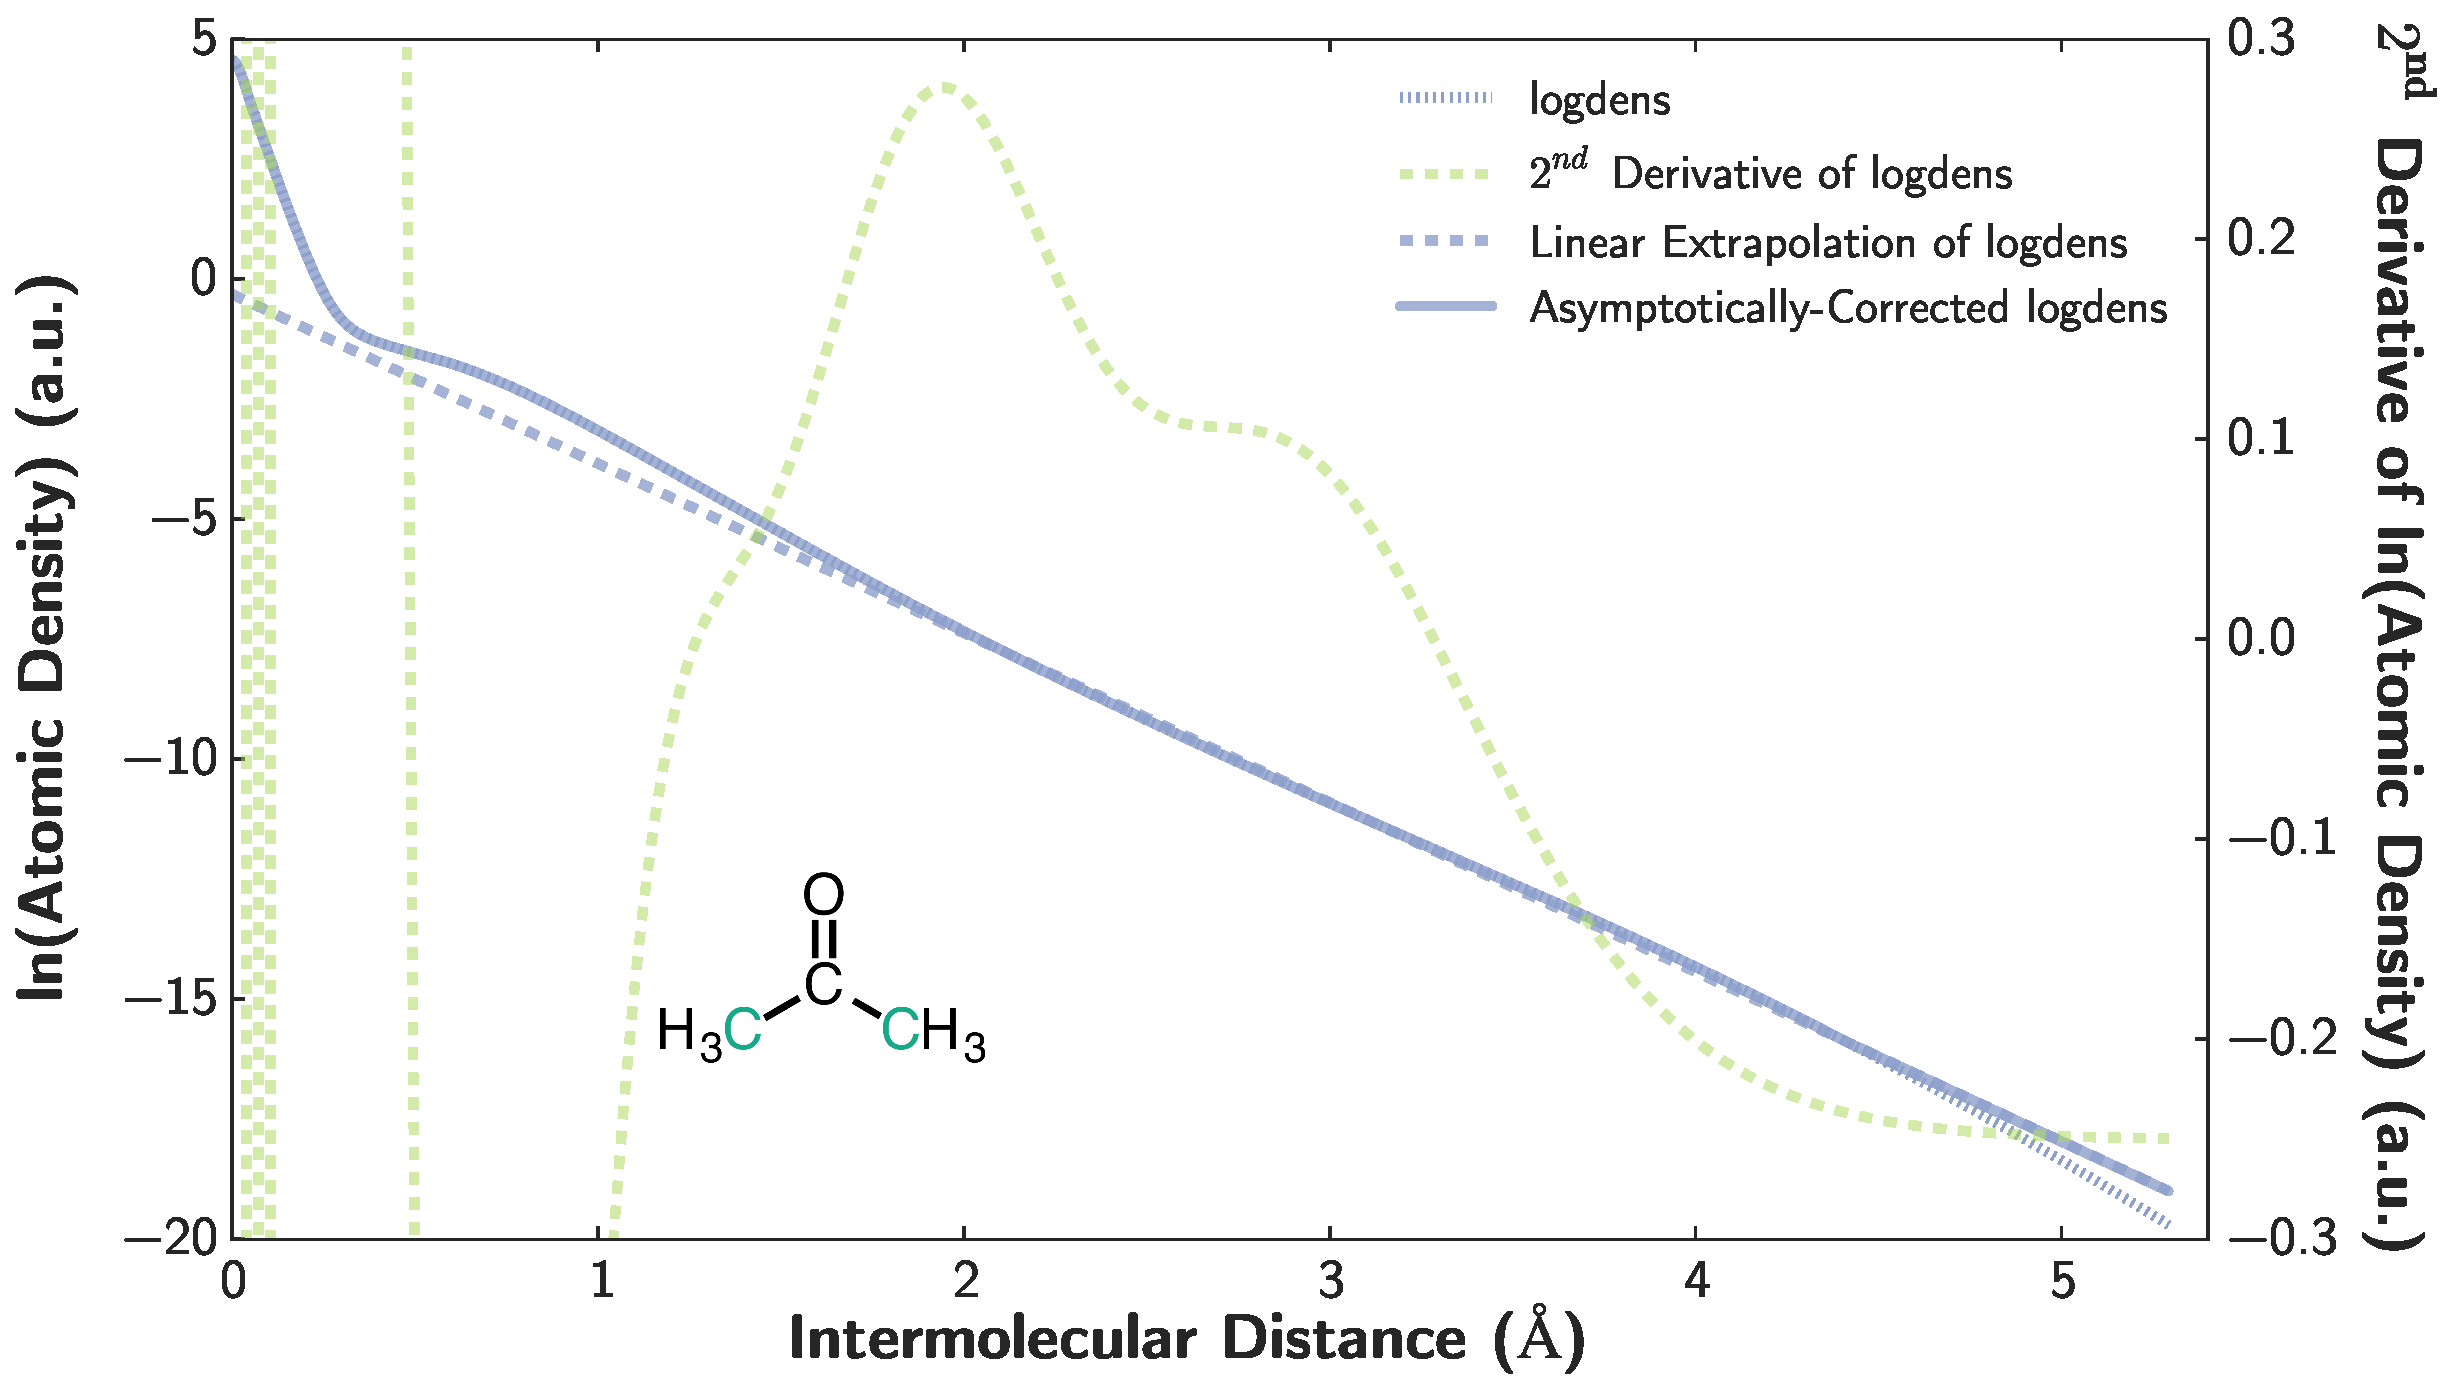
\includegraphics[width=0.9\textwidth]{isotropic/si/acetone_extrapolation.pdf}
%%     \caption{
%%         Linear extrapolation algorithm for the methyl carbon in acetone.
%% Depicted are (in legend order) Steps \ref{step1}, \ref{step2}, \ref{step3},
%% and \ref{step4} in the extrapolation algorithm. Note that some portions of the
%% $2^{nd}$ derivative extend off the graph; also note that most of logdens
%% is located underneath the asymptotically-corrected curve.
%%            		  }
%%     \label{fig:acetone-extrapolation}        
%%     \end{figure}
%%     %%%%%%%%% Bij Combination Rule %%%%%%%%%%%
%% 
%% 
%% 
%% \end{section}
%% \clearpage
%% \begin{section}{Non-polarizable, point-charge Lennard-Jones Force Fields}
%% 
%% As described in the main text, a non-polarizable, rank 0 multipole version of
%% \ljff was fit in order to produce force fields most in line with popular
%% standard force fields. Results for this \ljff are shown in
%% \tabref{tab:lj_rmse}; unsurprisingly, these force fields are less accurate and
%% less transferable compared to \ljff in the main text, which includes
%% polarizability and higher-order multipole moments.
%% 
%% 
%% %%%%%%%%%%%%%%%%%%%%% Average LJ RMSE Table %%%%%%%%%%%%%%%%%%%%%%%%%%%%%%%%%%%
%% %\begin{landscape}
%% \begin{table}
%% \small
%% \centering
%% \renewcommand\arraystretch{1.1}
%% \begin{tabular}{@{}rcccc@{}}
%% \hline
%% \toprule
%% & \phantom{} &
%%   \multicolumn{1}{c}{Dimer-Specific Fits} &
%%   \phantom{ab} &
%%   \multicolumn{1}{c}{Transferable Fits} \\
%% %\cmidrule{2} \cmidrule{3}
%% 
%% %% Component & & \ljff-q0, $\lambda=0.1$ & \ljff-q2, $\lambda=0.1$ & \ljff-q2, $\lambda=2.0$ 
%% %%           & & \ljff-q0, $\lambda=0.1$ & \ljff-q2, $\lambda=0.1$ & \ljff-q2, $\lambda=2.0$ \\
%% %%           & & \ljff-q2,               & \ljff-q2,               & \ljff-q0,               
%% %%           & & \ljff-q2,               & \ljff-q2,               & \ljff-q0,               \\
%% %%           & &           $\lambda=2.0$ &           $\lambda=0.1$ &           $\lambda=0.1$ 
%% %%           & &           $\lambda=2.0$ &           $\lambda=0.1$ &           $\lambda=0.1$ \\
%%      & & \multicolumn{1}{c}{(kJ mol$^{-1}$)} 
%%      & & \multicolumn{1}{c}{(kJ mol$^{-1}$)} \\
%% \midrule
%% %\addlinespace
%% %\textbf{
%% %Total Energy}   \\
%% %\emph{RMSE}             & &  1.984 (0.603)   &  6.058 (0.413)  &  5.116 (0.560)   && 2.054 (0.640)  &  5.760 (0.457)  &  4.513 (0.658) \\
%% \emph{RMSE}             & &    5.116 (0.560)   &&   4.513 (0.658) \\
%% %\addlinespace
%% \emph{\mse}
%%                  %& &  0.322 (0.345)   &  1.610 (0.041)  &  0.803 (0.038)   && 0.311 (0.368)  &  1.410 (0.060)  &  0.562 (0.079) \\
%%                  & &    0.803 (0.038)   &&   0.562 (0.079) \\
%% \bottomrule
%% \hline
%% \end{tabular}
%% \caption{
%%     Comparison of characteristic RMSE and \mse over the 91 dimer test
%%     set for the non-polarizable, rank 0 multipole Lennard-Jones model. The LJ
%%     models are not parameterized on a component-by-component basis, thus
%%     RMSE/\mse values for only the total FF energy is shown.  `Attractive'
%%     errors, representing the average RMSE/\mse for the subset of points
%%     whose energies are net attractive ($\etot < 0$), are shown in parentheses to
%%     the right of the total average RMS errors. `Dimer-Specific Fits' and
%%     `Transferable Fits' are as in the main text.
%% 	}
%% \label{tab:lj_rmse}
%% \end{table}
%% \normalsize
%% %\end{landscape}
%% %%%%%%%%%%%%%%%%%%%%% Average LJ RMSE Table %%%%%%%%%%%%%%%%%%%%%%%%%%%%%%%%%%%
%% 
%% 
%% \end{section}
%% \begin{section}{Born-Mayer-sISA: Scale Factor Tests}
%% 
%% \begin{subsection}{Comparison to $S_{ij}$}
%% 
%% Exact $S_{ij}$ (\eqref{eq:simple_overlap} and \eqref{eq:complicated_overlap})
%% values were computed for various element pairs as in
%% \secref{sec:bij_combo_rule}. Born-Mayer overlaps of the form
%% %
%% \begin{align*}
%% S_{ij} &\approx K_{ij}\exp(-\xi B_{ij} \R) \\
%% \intertext{where}
%% K_{ij} &= \frac{K}{B^{3}_{ij}} \\
%% B_{ij} &= \sqrt{B_i B_j}
%% \end{align*}
%% %
%% were fit to these exact overlaps; $K$ and $\xi$ were optimized as universal
%% parameters by performing a log-weighted fit over the entire set of $S_{ij}$
%% values. 
%% 
%% %%%%%%%%%%%%%%%%%%%%% Optimized S_IJ parameters Table %%%%%%%%%%%%%%%%%%%%%%%%%%%%%%%%%%%
%% \begin{table}
%% \small
%% \centering
%% \renewcommand\arraystretch{1.1}
%% \begin{tabular}{@{}rcccc@{}}
%% \hline
%% \toprule
%% Range of \R & \phantom{ab} & $\xi$ & \phantom{ab} & K \\
%% %% \multicolumn{5}{l}{(Fraction of Van der Waals radii for each atom pair)} \\
%% \midrule
%% {$[0.8,1.2]$} & & 0.738   & & 12.2  \\
%% {$[1.0,2.0]$} & & 0.812   & & 20.9  \\
%% {$[1.0,4.0]$} & & 0.878   & & 42.6  \\ 
%% 
%% \bottomrule
%% \hline
%% \end{tabular}
%% \caption{
%%     Optimized Born-Mayer parameters, $\xi$ and $K$, for fits to \\
%% $S_{ij} \approx \frac{K}{(B_iB_j)^{\sfrac32}}\exp(-\xi \sqrt{B_iB_j} \R)$.
%% $B_i$ and $B_j$ values have been chosen as in \ref{sec:bij_combo_rule}.
%% Tabulated \R ranges are expressed as a fraction of the sum of van der Waals
%% radii for atoms $i$ and $j$.
%% 	}
%% \label{tab:sij_scale_factor}
%% \end{table}
%% \normalsize
%% %%%%%%%%%%%%%%%%%%%%% Optimized S_IJ parameters Table %%%%%%%%%%%%%%%%%%%%%%%%%%%%%%%%%%%
%% 
%% Optimized parameters are shown in \ref{tab:sij_scale_factor} for various
%% ranges of \R.
%% As shown in
%% \ref{tab:sij_scale_factor}, the scale factor $\xi$ is highly sensitive to
%% the values of \R included in the fits, with larger values of \R tending to
%% increase $\xi$. On the other hand, $\xi$ is fairly insensitive to the
%% values of $B_i$ and $B_j$: setting $\xi = \xi_0 + \xi_1 B_{ij}$ does
%% not significantly improve fit quality. On the grounds of our overlap
%% tests, it is difficult to establish a precise value for $\xi$, though our
%% results do suggest that $\xi \sim 0.80$ and is largely independent of
%% the atomic exponents themselves.
%% 
%% \end{subsection}
%% \begin{subsection}{Comparison to \vtot}
%% 
%% Alternatively, we
%% optimized the \bmsisaff scale factor by minimizing errors in the force field 
%% itself. Average RMS errors for a variety of scale factors are shown in
%% \ref{tab:bmsisaff_scale_rmse}. Regardless of whether we consider each energy
%% component separately, or focus on the overall energy, setting $\xi=0.84$
%% is optimal; RMS errors for this choice are
%% comparable to the \isaffold itself.
%% 
%% %%%%%%%%%%%%%%%%%%%%% Average RMSE Table %%%%%%%%%%%%%%%%%%%%%%%%%%%%%%%%%%%
%% \begin{landscape}
%% \begin{table}
%% \small
%% \centering
%% \renewcommand\arraystretch{1.1}
%% \begin{tabular}{@{}rccccccc@{}}
%% \hline
%% \toprule
%% & \phantom{ab} &
%%   \multicolumn{6}{c}{Born-Mayer-sISA Scale Factor} 
%%   \\
%% \cmidrule{3-8}
%% 
%% Component & & $\xi= 0.80$ & $\xi= 0.82$ & $\xi= 0.84$ & $\xi= 0.86$ & $\xi = 0.88$ & $\xi = 0.90$  \\
%%      %% & & \multicolumn{1}{c}{(kJ mol$^{-1}$)} & \multicolumn{1}{c}{(kJ mol$^{-1}$)} &  \multicolumn{1}{c}{(kJ mol$^{-1}$)}
%%      %% & & \multicolumn{1}{c}{(kJ mol$^{-1}$)}& \multicolumn{1}{c}{(kJ mol$^{-1}$)} \\
%% \midrule
%% Exchange        & &  3.078 (0.697)   &    2.690 (0.668) &  2.677 (0.686)  & 2.841 (0.702)  &    3.225 (0.742)  &    3.798 (0.791) \\
%% Electrostatics  & &  1.144 (0.418)   &    1.105 (0.378) &  1.083 (0.352)  &    1.077 (0.342)  &    1.104 (0.354)  &    1.105 (0.373)  \\
%% Induction       & &  0.258 (0.099)   &    0.253 (0.097) &  0.250 (0.096)  &    0.246 (0.095)  &    0.243 (0.094)  &    0.240 (0.094)  \\
%% \dhf            & &  0.241 (0.072)   &    0.244 (0.069) &  0.248 (0.068)  &    0.255 (0.070)  &    0.263 (0.075)  &    0.272 (0.082)  \\
%% Dispersion      & &  0.934 (0.383)   &    0.803 (0.337) &  0.856 (0.336)  &    1.078 (0.370)  &    1.388 (0.426)  &    1.740 (0.496)  \\
%% \addlinespace                                                                                                                        
%% \textbf{                                                                                                                             
%% Total Energy}   & &  1.970 (0.503)   &    1.775 (0.455) &  1.751 (0.453)  &    1.818 (0.465)  &    2.084 (0.516)  &    2.451 (0.577) \\
%% \bottomrule
%% 
%% 
%% \hline
%% \end{tabular}
%% \caption{
%% 	Average RMS errors over the 91 dimer test set for \bmsisaff using different exponential scale factors. 
%% 	All quantities are in kJ mol$^{-1}$ except for scale factors, which are unitless.
%%     `Attractive' RMS errors, representing the average RMS error for
%%     the subset of points whose energies are net attractive (i.e., where $E_{tot} <
%%     0$), are shown in parentheses to the right of the total average RMS errors.
%%     Geometric (rather than arithmetic) averages are used in all cases.
%% 	}
%% \label{tab:bmsisaff_scale_rmse}
%% \end{table}
%% \normalsize
%% \end{landscape}
%% %%%%%%%%%%%%%%%%%%%%% Average RMSE Table %%%%%%%%%%%%%%%%%%%%%%%%%%%%%%%%%%%
%% 
%% \end{subsection}
%% 
%% \end{section}
%% \begin{section}{Slater-OPT and Born-Mayer-OPT Force Fields}
%% 
%% We developed a Slater-OPT force field,
%% identical to the \isaffold except that \B parameters were optimized to reproduce the
%% DFT-SAPT exchange-repulsion energy.
%% Analogously, we developed Born-Mayer-OPT as an
%% extension of the \bmsisaff. Treating \B as a completely
%% unconstrained parameter led to poor dispersion energies and overall
%% transferability, and was not considered further.
%% Instead, exponents were optimized using a harmonic
%% penalty function of the form $k(B-B_0)^2$, with $k=10^{-5}$ a.u.  For
%% Slater-OPT, $B_0$ values were taken from the \isaffold; for Born-Mayer-OPT, the \saptff
%% values were used. 
%% RMS errors for Slater-OPT and Born-Mayer-OPT are shown in
%% \ref{tab:bmopt_rmse}. 
%% For both Dimer-Specific and Transferable fits, Slater-OPT and Born-Mayer-OPT are
%% of comparable quality. Both force fields are only slight improvements to
%% either the \isaffold or the \bmsisaff; considering the extra number of free parameters
%% required to optimize atomic exponents, we consider these results further
%% confirmation of the inherent quality of the ISA exponents.
%% 
%% %%%%%%%%%%%%%%%%%%%%% Average RMSE Table %%%%%%%%%%%%%%%%%%%%%%%%%%%%%%%%%%%
%% %\begin{landscape}
%% \begin{table}
%% \small
%% \centering
%% \renewcommand\arraystretch{1.1}
%% \begin{tabular}{@{}rcccccc@{}}
%% \hline
%% \toprule
%% & \phantom{ab} &
%%   \multicolumn{2}{c}{Dimer-Specific Fits} &
%%   \phantom{ab} &
%%   \multicolumn{2}{c}{Transferable Fits} \\
%% \cmidrule{3-4} \cmidrule{6-7}
%% 
%% Component & & Slater-OPT & Born-Mayer-OPT & & Slater-OPT & Born-Mayer-OPT  \\
%%      & & \multicolumn{1}{c}{(kJ mol$^{-1}$)}  &  \multicolumn{1}{c}{(kJ mol$^{-1}$)}
%%      & & \multicolumn{1}{c}{(kJ mol$^{-1}$)}  &  \multicolumn{1}{c}{(kJ mol$^{-1}$)} \\
%% \midrule
%% Exchange        & &    2.513 (0.636)   &    2.433 (0.639)  & &    2.507 (0.665)  &   2.459 (0.671) \\
%% Electrostatics  & &    1.087 (0.362)   &    1.068 (0.352)  & &    1.129 (0.359)  &   1.113 (0.352) \\
%% Induction       & &    0.256 (0.097)   &    0.252 (0.096)  & &    0.282 (0.102)  &   0.280 (0.102) \\
%% \dhf            & &    0.241 (0.068)   &    0.244 (0.067)  & &    0.272 (0.077)  &   0.276 (0.077) \\
%% Dispersion      & &    0.836 (0.330)   &    0.822 (0.349)  & &    0.823 (0.331)  &   0.820 (0.350) \\
%% \addlinespace                                                                        
%% \textbf{                                                                
%% Total Energy}  \\ 
%% \emph{RMSE}
%%                 & &    1.549 (0.448)   &    1.597 (0.450)  & &    1.482 (0.454)  &   1.532 (0.458) \\
%% \emph{\mse}
%%                 & &    0.160 (0.065)   &    0.160 (0.084)  & &    0.149 (0.057)  &   0.204 (0.130) \\
%% \bottomrule
%% 
%% \hline
%% \end{tabular}
%% \caption{
%%     Comparison of geometric mean RMS errors over the 91 dimer test
%%     set for the Slater-OPT and Born-Mayer-OPT methods.
%%     `Attractive' RMS errors, representing the average RMS
%%     error for the subset of points whose energies are net attractive ($\etot < 0$), 
%%     are shown in parentheses to the right of the total average RMS errors.
%% 	}
%% \label{tab:bmopt_rmse}
%% \end{table}
%% \normalsize
%% %\end{landscape}
%% %%%%%%%%%%%%%%%%%%%%% Average RMSE Table %%%%%%%%%%%%%%%%%%%%%%%%%%%%%%%%%%%
%% 
%% 
%% 
%% 
%% \end{section}
%% 
%% 
%% \begin{section}{Monomer Geometries}
%% 
%% Geometries for each molecule in the 91 dimer test set are listed below, in
%% alphabetical order. Also listed are the relevant energies (highest occupied
%% molecular orbital and ionization potential) for the asymptotic correction
%% required in DFT-SAPT calculations of each molecule. All asymptotic corrections
%% were performed at a PBE0/\avtz level of theory. Distances and energies are in
%% a.u.
%% 
%% \scriptsize
%% \centering
\renewcommand\arraystretch{1.1}
\newcolumntype{L}{D{.}{.}{2,6}}
\begin{longtable}{@{}rLLL@{}}
\caption{Cartesian coordinates for each molecule in the 91 dimer test set. HOMO
and I.P. values, necessary for DFT-SAPT calculations, are also shown. All units
are in a.u.}
\label{tab:geometries}
\\

\endfirsthead

\multicolumn{4}{c}%
{{\bfseries \tablename\ \thetable{} -- continued from previous page}} \\
\hline
\endhead
%% \toprule
%% Atomtype & 
%% \multicolumn{1}{c}{$Q_{00 }$} &
%% \multicolumn{1}{c}{$Q_{10 }$} &
%% \multicolumn{1}{c}{$Q_{11c}$} &
%% \multicolumn{1}{c}{$Q_{11s}$} &
%% \multicolumn{1}{c}{$Q_{20 }$} &
%% \multicolumn{1}{c}{$Q_{21c}$} &
%% \multicolumn{1}{c}{$Q_{21s}$} &
%% \multicolumn{1}{c}{$Q_{22c}$} &
%% \multicolumn{1}{c}{$Q_{22s}$} \\
%% \midrule
%% \endhead
%% 
%% \bottomrule
%% \endfoot

\multicolumn{4}{l}{\textbf{Acetone}}  \\*
\toprule
\input{acetone_geometry.tex}
\bottomrule
\multicolumn{2}{l}{HOMO:} &
-0.266741       
\\*
\multicolumn{2}{l}{I.P.:} &
0.35386979
\\*
\\

\multicolumn{4}{l}{\textbf{Ar}}  \\*
\toprule
\input{ar_geometry.tex}
\bottomrule
\multicolumn{2}{l}{HOMO:} &
-0.440599       
\\*
\multicolumn{2}{l}{I.P.:} &
0.58049447
\\*
\\

\multicolumn{4}{l}{\textbf{Chloromethane}}  \\*
\toprule
\input{chloromethane_geometry.tex}
\bottomrule
\multicolumn{2}{l}{HOMO:} &
-0.313074       
\\*
\multicolumn{2}{l}{I.P.:} &
0.41507894
\\*
\\

\multicolumn{4}{l}{\textbf{CO\sub2}}  \\*
\toprule
\input{co2_geometry.tex}
\bottomrule
\multicolumn{2}{l}{HOMO:} &
-0.394037       
\\*
\multicolumn{2}{l}{I.P.:} &
0.51235857
\\*
\\

\multicolumn{4}{l}{\textbf{Dimethyl Ether}}  \\*
\toprule
\input{dimethyl_ether_geometry.tex}
\bottomrule
\multicolumn{2}{l}{HOMO:} &
-0.272835       
\\*
\multicolumn{2}{l}{I.P.:} &
0.36469012
\\*
\\

\multicolumn{4}{l}{\textbf{Ethane}}  \\*
\toprule
\input{ethane_geometry.tex}
\bottomrule
\multicolumn{2}{l}{HOMO:} &
-0.353672       
\\*
\multicolumn{2}{l}{I.P.:} &
0.45125450
\\*
\\

\multicolumn{4}{l}{\textbf{Ethanol}}  \\*
\toprule
\input{ethanol_geometry.tex}
\bottomrule
\multicolumn{2}{l}{HOMO:} &
-0.287342       
\\*
\multicolumn{2}{l}{I.P.:} &
0.38582676
\\*
\\

\multicolumn{4}{l}{\textbf{Ethene}}  \\*
\toprule
\input{ethene_geometry.tex}
\bottomrule
\multicolumn{2}{l}{HOMO:} &
-0.288580       
\\*
\multicolumn{2}{l}{I.P.:} &
0.38518748
\\*
\\

\multicolumn{4}{l}{\textbf{H\sub2O}}  \\*
\toprule
\input{h2o_geometry.tex}
\bottomrule
\multicolumn{2}{l}{HOMO:} &
-0.333820       
\\*
\multicolumn{2}{l}{I.P.:} &
0.46592291
\\*
\\

\multicolumn{4}{l}{\textbf{Methane}}  \\*
\toprule
\input{methane_geometry.tex}
\bottomrule
\multicolumn{2}{l}{HOMO:} &
-0.403996       
\\*
\multicolumn{2}{l}{I.P.:} &
0.51955025
\\*
\\

\multicolumn{4}{l}{\textbf{Methanol}}  \\*
\toprule
\input{methanol_geometry.tex}
\bottomrule
\multicolumn{2}{l}{HOMO:} &
-0.292049       
\\*
\multicolumn{2}{l}{I.P.:} &
0.39901686
\\*
\\

\multicolumn{4}{l}{\textbf{Methyl Amine}}  \\*
\toprule
\input{methyl_amine_geometry.tex}
\bottomrule
\multicolumn{2}{l}{HOMO:} &
-0.255840       
\\*
\multicolumn{2}{l}{I.P.:} &
0.35552078
\\*
\\

\multicolumn{4}{l}{\textbf{NH\sub3}}  \\*
\toprule
\input{nh3_geometry.tex}
\bottomrule
\multicolumn{2}{l}{HOMO:} &
-0.284421       
\\*
\multicolumn{2}{l}{I.P.:} &
0.39987353
\\*
\\


\end{longtable}



%% \normalsize
%% 
%% 
%% \end{section}
%% \begin{section}{Homomonomeric Parameters}
%% 
%% 
%% Parameters for each molecule (as fit to homomonomeric dimers) are given
%% for the \isaffold, the \saptff, and the \bmsisaff. Multipole moments are listed in
%% the first subsection, as these values are identical for all
%% force fields. The next subsections list $A_i$, $B_{i}$, $C_{i,n}$
%% parameters for each atom type in each molecule, as well as Drude oscillator
%% charges $Q_{drude}$.
%% 
%% \begin{subsection}{Multipole Moments}
%% 
%% Multipole moments for each atom in each molecule are listed in
%% \ref{tab:multipoles}. Multipoles are expressed in spherical form
%% following notation used by \citeauthor{stone2013theory}.\cite{stone2013theory}
%% Note that the global coordinate system is used, with molecular geometries as
%% in \ref{tab:geometries}. 
%% 
%% \scriptsize
%% \centering
\renewcommand\arraystretch{1.1}
\newcolumntype{L}{D{.}{.}{2,6}}
\begin{longtable}{@{}rLLLLLLLLL@{}}
\caption{Multipole moments for each molecule in the 91 dimer test set.}
\label{tab:multipoles}
\\

\toprule
Atomtype & 
\multicolumn{1}{c}{$Q_{00 }$} &
\multicolumn{1}{c}{$Q_{10 }$} &
\multicolumn{1}{c}{$Q_{11c}$} &
\multicolumn{1}{c}{$Q_{11s}$} &
\multicolumn{1}{c}{$Q_{20 }$} &
\multicolumn{1}{c}{$Q_{21c}$} &
\multicolumn{1}{c}{$Q_{21s}$} &
\multicolumn{1}{c}{$Q_{22c}$} &
\multicolumn{1}{c}{$Q_{22s}$} \\
\midrule
\endfirsthead

\multicolumn{10}{c}%
{{\bfseries \tablename\ \thetable{} -- continued from previous page}} \\
\toprule
Atomtype & 
\multicolumn{1}{c}{$Q_{00 }$} &
\multicolumn{1}{c}{$Q_{10 }$} &
\multicolumn{1}{c}{$Q_{11c}$} &
\multicolumn{1}{c}{$Q_{11s}$} &
\multicolumn{1}{c}{$Q_{20 }$} &
\multicolumn{1}{c}{$Q_{21c}$} &
\multicolumn{1}{c}{$Q_{21s}$} &
\multicolumn{1}{c}{$Q_{22c}$} &
\multicolumn{1}{c}{$Q_{22s}$} \\
\midrule
\endhead

\addlinespace
\bottomrule
\endfoot

\addlinespace
\multicolumn{4}{l}{\textbf{Acetone}}  \\*
\input{isotropic/si/acetone_mom.tex}

\addlinespace
\multicolumn{4}{l}{\textbf{Ar}}  \\*
\input{isotropic/si/ar_mom.tex}

\addlinespace
\multicolumn{4}{l}{\textbf{Chloromethane}}  \\*
\input{isotropic/si/chloromethane_mom.tex}

\addlinespace
\multicolumn{4}{l}{\textbf{\co}}  \\*
\input{isotropic/si/co2_mom.tex}

\addlinespace
\multicolumn{4}{l}{\textbf{Dimethyl Ether}}  \\*
\input{isotropic/si/dimethyl_ether_mom.tex}

\addlinespace
\multicolumn{4}{l}{\textbf{Ethane}}  \\*
\input{isotropic/si/ethane_mom.tex}

\addlinespace
\multicolumn{4}{l}{\textbf{Ethanol}}  \\*
\input{isotropic/si/ethanol_mom.tex}

\addlinespace
\multicolumn{4}{l}{\textbf{Ethene}}  \\*
\input{isotropic/si/ethene_mom.tex}

\addlinespace
\multicolumn{4}{l}{\textbf{\co}}  \\*
\input{isotropic/si/h2o_mom.tex}

\addlinespace
\multicolumn{4}{l}{\textbf{Methane}}  \\*
\input{isotropic/si/methane_mom.tex}

\addlinespace
\multicolumn{4}{l}{\textbf{Methanol}}  \\*
\input{isotropic/si/methanol_mom.tex}

\addlinespace
\multicolumn{4}{l}{\textbf{Methyl Amine}}  \\*
\input{isotropic/si/methyl_amine_mom.tex}

\addlinespace
\multicolumn{4}{l}{\textbf{\nh}}  \\*
\input{isotropic/si/nh3_mom.tex}


\end{longtable}


%% C  &  0.0000  & 0.0000  &  0.1880    \\
%% O  &  0.0000  & 0.0000  &  1.3947    \\
%% C  &  0.0000  & 1.2886  &  -0.6129   \\
%% C  &  0.0000  & -1.2886 &  -0.6129   \\
%% H  &  0.0000  & 2.1434  &  0.0583    \\
%% H  &  0.0000  & -2.1434 &  0.0583    \\
%% H  &  0.8772  & 1.3305  &  -1.2617   \\
%% H  &  -0.8772 & 1.3305  &  -1.2617   \\
%% H  &  -0.8772 & -1.3305 &  -1.2617   \\
%% H  &   0.8772 & -1.3305 &  -1.2617   \\
%%                                        
%%                                        
%% Ar &  0.0000  & 0.0000  &  0.0000    \\
%%                                        
%%                                        
%% C  &  0.0000  & 0.0000  &  -1.5159   \\
%% Br &  0.0000  & 0.0000  &  0.4181    \\
%% H  &  0.0000  & 1.0309  &  -1.8455   \\
%% H  &  0.8928  & -0.5155 &  -1.8455   \\
%% H  &  -0.8928 & -0.5155 &  -1.8455   \\
%%                                        
%%                                                                   
%% C  &  0.0000  & 0.0000  &  0.0000    \\
%% Cl &  0.0000  & 0.0000  &  1.7810    \\
%% H  &  1.0424  & 0.0000  &  -0.3901   \\
%% H  &  -0.5212 & 0.9027  &  -0.3901   \\
%% H  &  -0.5212 & -0.9027 &  -0.3901   \\
%%                                        
%%                                                                   
%% C  &  0.0000  & 0.0000  &  0.0000    \\
%% O  &  0.0000  & 0.0000  &  1.1621    \\
%% O  &  0.0000  & 0.0000  &  -1.1621   \\
%%                                        
%%                                                                           
%% O  &  0.0000  & 0.0000  &  0.5952    \\
%% C  &  0.0000  & 1.1669  &  -0.1963   \\
%% C  &  0.0000  & -1.1669 &  -0.1963   \\
%% H  &  0.0000  & 2.0489  &  0.4542    \\
%% H  &  0.0000  & -2.0489 &  0.4542    \\
%% H  &  0.8950  & 1.1787  &  -0.8287   \\
%% H  &  -0.8950 & 1.1787  &  -0.8287   \\
%% H  &  -0.8950 & -1.1787 &  -0.8287   \\
%% H  &  0.8950  & -1.1787 &  -0.8287   \\
%%                                        
%%                                                                   
%% C  &  0.0000  & 0.0000  &  0.7680    \\
%% C  &  0.0000  & 0.0000  &  -0.7680   \\
%% H  &  -1.0192 & 0.0000  &  1.1573    \\
%% H  &  0.5096  & 0.8826  &  1.1573    \\
%% H  &  0.5096  & -0.8826 &  1.1573    \\
%% H  &  1.0192  & 0.0000  &  -1.1573   \\
%% H  &  -0.5096 & -0.8826 &  -1.1573   \\
%% H  &  -0.5096 & 0.8826  &  -1.1573   \\
%%                                        
%%                                                                    
%% C  &  1.1879  & -0.3829 &  0.0000    \\
%% C  &  0.0000  & 0.5526  &  0.0000    \\
%% O  &  -1.1867 & -0.2472 &  0.0000    \\
%% H  &  -1.9237 & 0.3850  &  0.0000    \\
%% H  &  2.0985  & 0.2306  &  0.0000    \\
%% H  &  1.1184  & -1.0093 &  0.8869    \\
%% H  &  1.1184  & -1.0093 &  -0.8869   \\
%% H  &  -0.0227 & 1.1812  &  0.8852    \\
%% H  &  -0.0227 & 1.1812  &  -0.8852   \\
%%                                        
%%                                                                   
%% C  &  0.0000  & 0.0000  &  0.6695    \\
%% C  &  0.0000  & 0.0000  &  -0.6695   \\
%% H  &  0.0000  & 0.9289  &  1.2321    \\
%% H  &  0.0000  & -0.9289 &  1.2321    \\
%% H  &  0.0000  & 0.9289  &  -1.2321   \\
%% H  &  0.0000  & -0.9289 &  -1.2321   \\
%%                                        
%%                                                                  
%% O  &  0.0000  & 0.0000  &  0.1173    \\
%% H  &  0.0000  & 0.7572  &  -0.4692   \\
%% H  &  0.0000  & -0.7572 &  -0.4692   \\
%%                                        
%%                                                                    
%% C  &  0.0000  & 0.0000  &  0.0000    \\
%% H  &  0.6276  & 0.6276  &  0.6276    \\
%% H  &  0.6276  & -0.6276 &  -0.6276   \\
%% H  &  -0.6276 & 0.6276  &  -0.6276   \\
%% H  &  -0.6276 & -0.6276 &  0.6276    \\
%%                                        
%%                                                                     
%% C  &  -0.0503 & 0.6685  &  0.0000    \\
%% O  &  -0.0503 & -0.7585 &  0.0000    \\
%% H  &  -1.0807 & 1.0417  &  0.0000    \\
%% H  &  0.4650  & 1.0417  &  0.8924    \\
%% H  &  0.4650  & 1.0417  &  -0.8924   \\
%% H  &  0.8544  & -1.0677 &  0.0000    \\
%%                                        
%%                                                                            
%% C  &  0.0516  & 0.7071  &  0.0000    \\
%% N  &  0.0516  & -0.7640 &  0.0000    \\
%% H  &  -0.9474 & 1.1766  &  0.0000    \\
%% H  &  0.5950  & 1.0631  &  0.8831    \\
%% H  &  0.5950  & 1.0631  &  -0.8831   \\
%% H  &  -0.4565 & -1.0985 &  -0.8137   \\
%% H  &  -0.4565 & -1.0985 &  0.8137    \\
%%                                        
%%                                                                    
%% N  &  0.0000  & 0.0000  &  0.0000    \\
%% H  &  0.0000  & -0.9377 &  -0.3816   \\
%% H  &  0.8121  & 0.4689  &  -0.3816   \\
%% H  &  -0.8121 & 0.4689  &  -0.3816   \\
%% 

%% \normalsize
%% 
%% \end{subsection}
%% \clearpage
%% \begin{subsection}{\isaffold Parameters}
%% 
%% $A_i$, $B_i$, $C_{i,n}$ parameters for the \isaffold are listed in \ref{tab:isaffold}.
%% \A, \B, and $C_{ij,n}$ parameters can be determined from the following
%% combination rules:
%% \begin{align*}
%% \A &= A_iA_j \\
%% \B &= \sqrt{B_iB_j} \\
%% C_{ij,n} &= \sqrt{C_{i,n}C_{j,n}}
%% \end{align*}
%% %
%% Parameters are given for each unique atom type in each molecule; where
%% multiple atom types exist for a particular element, atom types are labeled 
%% first with the element name and second by connectivity. Thus the carbonyl
%% carbon in acetone is labeled `CO', whereas the methyl carbon is labeled `CH'.
%% 
%% The total force field energy is defined by the following equations:
%% %
%% \begin{align*}
%% B_i &= B_i^{ISA} \\
%% P(B_{ij},r_{ij}) &= \frac13 (B_{ij} r_{ij})^2 + B_{ij} r_{ij} + 1 \\
%% x &= B_{ij}r_{ij} - \frac{2 B_{ij}^2 r_{ij} + 3 B_{ij} }
%% { B_{ij}^2 r_{ij}^2 + 3 B_{ij} r_{ij} + 3} r_{ij} \\
%% f_{2n}(x) &= 1 - e^{-x} \sum \limits_{k=0}^{2n} \frac{(x)^k}{k!} \\
%% \vrep_{ij} &= A_{ij}^{exch} P(B_{ij}, r_{ij}) \exp(-B_{ij}r_{ij}) \\
%% \velst_{ij} &= -A_{ij}^{elst} P(B_{ij}, r_{ij}) \exp(-B_{ij}r_{ij}) + \vmultipole \\
%% \vind_{ij} &= -A_{ij}^{ind} P(B_{ij}, r_{ij}) \exp(-B_{ij}r_{ij}) + \vdrudeind \\
%% \vdhf_{ij} &= -A_{ij}^{\dhf} P(B_{ij}, r_{ij}) \exp(-B_{ij}r_{ij}) +
%% \vdrudescf \\
%% \vdisp_{ij} &= - \sum\limits_{n=3}^{6} f_{2n}(x) \frac{C_{ij,2n}}{r_{ij}^{2n}} \\
%% \\
%% \vtot &= \sum\limits_{ij} \velst_{ij} + \vrep_{ij} + \vind_{ij} + \vdhf_{ij} + \vdisp_{ij}
%% \end{align*}
%% %
%% The Tang-Toennies damping function $f$ is defined in the main text; the
%% polarization energy $\vdrude = \vdrudeind + \vdrudescf$ arising from drude oscillators is defined in
%% \citen{Yu2011}.
%% 
%% \scriptsize
%% \input{all_isaffold_params.tex}
%% \normalsize
%% 
%% \end{subsection}
%% \clearpage
%% \begin{subsection}{\saptff Parameters}
%% 
%% $A_i$, $B_i$, $C_{i,n}$ parameters for the \saptff are listed in \ref{tab:saptff}.
%% \A, \B, and $C_{ij,n}$ parameters can be determined from the following
%% combination rules:
%% \begin{align*}
%% \A &= A_iA_j \\
%% \B &= \frac{B_iB_j(B_i + B_j)}{B_i^2 + B_j^2} \\
%% C_{ij,n} &= \sqrt{C_{i,n}C_{j,n}}
%% \end{align*}
%% %
%% Parameters are given for each unique atom type in each molecule; where
%% multiple atom types exist for a particular element, atom types are labeled 
%% first with the element name and second by connectivity. Thus the carbonyl
%% carbon in acetone is labeled `CO', whereas the methyl carbon is labeled `CH'.
%% 
%% The total force field energy is defined by the following equations:
%% %
%% \begin{align*}
%% B_i &= 2\sqrt{2IP_i} \\
%% P(B_{ij},r_{ij}) &= 1 \\
%% x &= B_{ij}r_{ij} \\
%% f_{2n}(x) &= 1 - e^{-x} \sum \limits_{k=0}^{2n} \frac{(x)^k}{k!} \\
%% \vrep_{ij} &= A_{ij}^{exch} P(B_{ij}, r_{ij}) \exp(-B_{ij}r_{ij}) \\
%% \velst_{ij} &= -A_{ij}^{elst} P(B_{ij}, r_{ij}) \exp(-B_{ij}r_{ij}) + \vmultipole \\
%% \vind_{ij} &= -A_{ij}^{ind} P(B_{ij}, r_{ij}) \exp(-B_{ij}r_{ij}) + \vdrudeind \\
%% \vdhf_{ij} &= -A_{ij}^{\dhf} P(B_{ij}, r_{ij}) \exp(-B_{ij}r_{ij}) +
%% \vdrudescf \\
%% \vdisp_{ij} &= - \sum\limits_{n=3}^{6} f_{2n}(x) \frac{C_{ij,2n}}{r_{ij}^{2n}} \\
%% \\
%% \vtot &= \sum\limits_{ij} \velst_{ij} + \vrep_{ij} + \vind_{ij} + \vdhf_{ij} +
%% \vdisp_{ij}
%% \end{align*}
%% %
%% The Tang-Toennies damping function $f$ is defined in the main text; the
%% polarization energy $E_{pol}$ arising from drude oscillators is defined in
%% \citen{Yu2011}.
%% 
%% \scriptsize
%% \newcolumntype{L}{D{.}{.}{2,6}}
\newcolumntype{C}{D{.}{.}{2,3}}
\newcolumntype{d}{D{.}{.}{4,3}}
\newcolumntype{E}{D{.}{.}{5,3}}
\newcolumntype{F}{D{.}{.}{6,3}}
\newcolumntype{Q}{D{.}{.}{2,4}}
\begin{center}
\begin{longtable}{@{}rLLLLLCdEFQ@{}}
\caption{\saptff parameters.}
\label{tab:saptff}
\\


\toprule
%Atomtype & $A_{exch}$ & $A_{elst}$  & $A_{ind}$ & $A_{\deltaHF}$ & $B$ & $C_6$ &  $C_8$ & $C_{10}$ & $C_{12}$  & $Q_{drude}$ \\
Atomtype & 
\multicolumn{1}{c}{$A_{exch}$}  & 
\multicolumn{1}{c}{$A_{elst}$}   & 
\multicolumn{1}{c}{$A_{ind}$} & 
\multicolumn{1}{c}{$A_{\delta HF}$} & 
\multicolumn{1}{c}{$B$} & 
\multicolumn{1}{c}{$C_6$} &  
\multicolumn{1}{c}{$C_8$} & 
\multicolumn{1}{c}{$C_{10}$} & 
\multicolumn{1}{c}{$C_{12}$}  & 
\multicolumn{1}{c}{$Q_{drude}$} \\
\midrule
\endfirsthead

\multicolumn{11}{c}%
{{\bfseries \tablename\ \thetable{} -- continued from previous page}} \\
\toprule
%Atomtype & $A_{exch}$ & $A_{elst}$  & $A_{ind}$ & $A_{\deltaHF}$ & $B$ & $C_6$ &  $C_8$ & $C_{10}$ & $C_{12}$  & $Q_{drude}$ \\
Atomtype & 
\multicolumn{1}{c}{$A_{exch}$}  & 
\multicolumn{1}{c}{$A_{elst}$}   & 
\multicolumn{1}{c}{$A_{ind}$} & 
\multicolumn{1}{c}{$A_{\delta HF}$} & 
\multicolumn{1}{c}{$B$} & 
\multicolumn{1}{c}{$C_6$} &  
\multicolumn{1}{c}{$C_8$} & 
\multicolumn{1}{c}{$C_{10}$} & 
\multicolumn{1}{c}{$C_{12}$}  & 
\multicolumn{1}{c}{$Q_{drude}$} \\
\midrule
\endhead

\bottomrule
\endfoot

\multicolumn{3}{l}{\textbf{Acetone}}  \\
CO    & 5.567455  & 2.919090  & 2.729352  & 0.705232  & 1.819469  &    13.406 &   145.511 &  6091.546 & 80859.461      & -0.4541 \\
OC    & 12.941114  & 8.025300  & 0.409461  & 3.556175  & 2.000912  &    22.881 &   353.876 & 10131.697 & 174478.272    & -0.9327 \\
CH    & 10.952564  & 6.356726  & 0.000000  & 0.230007  & 1.819469  &    23.494 &   353.376 &  4001.387 & 41152.121     & -1.2947 \\
HC    & 2.111731  & 1.047688  & 0.616407  & 0.767149  & 1.999464  &     2.245 &    42.098 &  1104.938 &     0.000      & 0.0000 \\
\addlinespace

\multicolumn{3}{l}{\textbf{Ar}}  \\
Ar    & 50.711700  & 26.176317  & 5.968585  & 9.099102  & 2.152496  &    71.007 &  1556.382 & 37687.507 & 709695.360   & -1.0694 \\
\addlinespace

\multicolumn{3}{l}{\textbf{Chloromethane}}  \\
H     & 1.773426  & 0.876699  & 0.418998  & 0.906852  & 1.999464  &     2.245 &    42.098 &  1104.938 &     0.000       & 0.0000 \\
C     & 12.813654  & 7.191403  & 1.079346  & 0.000000  & 1.819469  &    23.494 &   353.376 &  4001.387 & 41152.121      & -1.2833 \\
Cl    & 34.276817  & 20.817366  & 7.997654  & 5.798695  & 1.952538  &    93.240 &  1615.853 & 65715.929 & 1310829.439   & -1.2661 \\
\addlinespace

\multicolumn{3}{l}{\textbf{\co}}  \\
C     & 5.176487  & 2.984618  & 2.277174  & 0.274561  & 1.819469  &    19.902 &   392.050 &  6560.549 & 144984.178     & -0.8645 \\
O     & 11.349651  & 6.499242  & 0.865006  & 2.716049  & 2.000912  &    15.043 &   264.275 &  6361.827 & 104726.425    & -0.7611 \\
\addlinespace

\multicolumn{3}{l}{\textbf{Dimethyl Ether}}  \\
H     & 2.329781  & 1.183750  & 0.564499  & 0.806639  & 1.999464  &     2.245 &    42.098 &  1104.938 &     0.000      & 0.0000 \\
C     & 8.563364  & 4.968189  & 0.131071  & 0.074779  & 1.819469  &    23.494 &   353.376 &  4001.387 & 41152.121      & -1.3211 \\
O     & 11.989376  & 7.808839  & 1.317489  & 3.114127  & 2.000912  &    12.235 &   266.573 &  6615.160 & 125669.048    & -0.0001 \\
\addlinespace

\multicolumn{3}{l}{\textbf{Ethane}}  \\
H     & 2.250973  & 1.158733  & 0.485471  & 0.781917  & 1.999464  &     2.245 &    42.098 &  1104.938 &     0.000     & 0.0000 \\
C     & 10.461511  & 5.586592  & 0.612844  & 0.406278  & 1.819469  &    23.494 &   353.376 &  4001.387 & 41152.121    & -1.2959 \\
\addlinespace

\multicolumn{3}{l}{\textbf{Ethanol}}  \\
CO    & 8.222663  & 5.833862  & 0.000000  & 0.000000  & 1.819469  &    23.494 &   353.376 &  4001.387 & 41152.121     & -1.2545 \\
OH    & 13.923864  & 8.979075  & 0.940969  & 3.229934  & 2.000912  &    14.592 &   320.063 &  8074.269 & 154258.592   & -0.8362 \\
HC    & 2.149784  & 1.068436  & 0.570784  & 0.766874  & 1.999464  &     2.245 &    42.098 &  1104.938 &     0.000     & 0.0000 \\
HO    & 1.019177  & 0.356079  & 0.751733  & 0.328847  & 1.999464  &     1.627 &    16.150 &   918.236 &     0.000     & 0.0000 \\
CH    & 10.141256  & 5.806452  & 0.278019  & 0.593277  & 1.819469  &    23.494 &   353.376 &  4001.387 & 41152.121    & -1.1875 \\
\addlinespace

\multicolumn{3}{l}{\textbf{Ethene}}  \\
C     & 15.765638  & 9.111034  & 1.960627  & 2.997793  & 1.819469  &    28.252 &   422.533 &  9835.457 & 152927.660   & -1.2627 \\
H     & 1.601044  & 0.584328  & 0.335499  & 0.611640  & 1.999464  &     2.245 &    42.098 &  1104.938 &     0.000     & 0.0000 \\
\addlinespace

\multicolumn{3}{l}{\textbf{\ho}}  \\
H     & 1.141499  & 0.446043  & 0.697274  & 0.318684  & 1.999464  &     0.776 &     3.042 &   270.370 &     0.000      & 0.0000 \\
O     & 13.932606  & 9.201940  & 0.282581  & 2.951132  & 2.000912  &    25.358 &   536.662 & 12267.338 & 220953.821    & -0.9794 \\
\addlinespace

\multicolumn{3}{l}{\textbf{Methane}}  \\
C     & 11.713473  & 6.761088  & 0.527832  & 0.632892  & 1.819469  &    23.494 &   353.376 &  4001.387 & 41152.121    & -1.2959 \\
H     & 2.225001  & 1.035042  & 0.508080  & 0.739327  & 1.999464  &     2.245 &    42.098 &  1104.938 &     0.000     & 0.0000 \\
\addlinespace

\multicolumn{3}{l}{\textbf{Methanol}}  \\
CO    & 7.433631  & 4.180536  & 0.401704  & 0.000000  & 1.819469  &    23.494 &   353.376 &  4001.387 & 41152.121      & -1.2724 \\
OH    & 13.542794  & 8.726014  & 0.795157  & 3.058222  & 2.000912  &    14.592 &   320.063 &  8074.269 & 154258.592    & -0.8102 \\
HO    & 0.922058  & 0.309528  & 0.702616  & 0.306417  & 1.999464  &     1.627 &    16.150 &   918.236 &     0.000      & 0.0000 \\
HC    & 2.230349  & 1.176985  & 0.567045  & 0.789220  & 1.999464  &     2.245 &    42.098 &  1104.938 &     0.000      & 0.0000 \\
\addlinespace

\multicolumn{3}{l}{\textbf{Methyl Amine}}  \\
HN    & 1.224682  & 0.421352  & 0.547503  & 0.429622  & 1.999464  &     1.627 &    16.150 &   918.236 &     0.000      & 0.0000 \\
N     & 23.338368  & 15.290981  & 1.429713  & 4.422039  & 2.067111  &    22.664 &   623.023 & 19359.417 & 472166.465   & -1.1026 \\
C     & 10.818390  & 6.130391  & 0.375108  & 0.000000  & 1.819469  &    23.494 &   353.376 &  4001.387 & 41152.121     & -1.2667 \\
HC    & 2.000843  & 1.025883  & 0.546828  & 0.808373  & 1.999464  &     2.245 &    42.098 &  1104.938 &     0.000      & 0.0000 \\
\addlinespace

\multicolumn{3}{l}{\textbf{\nh}}  \\
H     & 1.291205  & 0.567250  & 0.560466  & 0.444433  & 1.999464  &     1.627 &    16.150 &   918.236 &     0.000      & -1.1928 \\
N     & 23.837579  & 14.999330  & 0.902266  & 4.021003  & 2.067111  &    22.664 &   623.023 & 19359.417 & 472166.465   & 0.0000 \\
\addlinespace


\end{longtable}
\end{center}

%% \normalsize
%% %
%% \end{subsection}
%% \clearpage
%% \begin{subsection}{\bmsisaff Parameters}
%% 
%% $A_i$, $B_i$, $C_{i,n}$ parameters for the \bmsisaff are listed in \ref{tab:bmsisaff}.
%% \A, \B, and $C_{ij,n}$ parameters can be determined from the following
%% combination rules:
%% \begin{align*}
%% \A &= A_iA_j \\
%% \B &= \sqrt{B_iB_j} \\
%% C_{ij,n} &= \sqrt{C_{i,n}C_{j,n}}
%% \end{align*}
%% %
%% Parameters are given for each unique atom type in each molecule; where
%% multiple atom types exist for a particular element, atom types are labeled 
%% first with the element name and second by connectivity. Thus the carbonyl
%% carbon in acetone is labeled `CO', whereas the methyl carbon is labeled `CH'.
%% 
%% The total force field energy is defined by the following equations:
%% %
%% \begin{align*}
%% B_i &= 0.84B_i^{ISA} \\
%% P(B_{ij},r_{ij}) &= 1 \\
%% x &= B_{ij}r_{ij} \\
%% f_{2n}(x) &= 1 - e^{-x} \sum \limits_{k=0}^{2n} \frac{(x)^k}{k!} \\
%% \vrep_{ij} &= A_{ij}^{exch} P(B_{ij}, r_{ij}) \exp(-B_{ij}r_{ij}) \\
%% \velst_{ij} &= -A_{ij}^{elst} P(B_{ij}, r_{ij}) \exp(-B_{ij}r_{ij}) + \vmultipole \\
%% \vind_{ij} &= -A_{ij}^{ind} P(B_{ij}, r_{ij}) \exp(-B_{ij}r_{ij}) + \vdrudeind \\
%% \vdhf_{ij} &= -A_{ij}^{\dhf} P(B_{ij}, r_{ij}) \exp(-B_{ij}r_{ij}) +
%% \vdrudescf \\
%% \vdisp_{ij} &= - \sum\limits_{n=3}^{6} f_{2n}(x) \frac{C_{ij,2n}}{r_{ij}^{2n}} \\
%% \\
%% \vtot &= \sum\limits_{ij} \velst_{ij} + \vrep_{ij} + \vind_{ij} + \vdhf_{ij} + \vdisp_{ij}
%% \end{align*}
%% %
%% The Tang-Toennies damping function $f$ is defined in the main text; the
%% polarization energy $\vdrude = \vdrudeind + \vdrudescf$ arising from drude oscillators is defined in
%% \citen{Yu2011}.
%% 
%% \scriptsize
%% \newcolumntype{L}{D{.}{.}{2,6}}
\newcolumntype{C}{D{.}{.}{2,3}}
\newcolumntype{d}{D{.}{.}{4,3}}
\newcolumntype{E}{D{.}{.}{5,3}}
\newcolumntype{F}{D{.}{.}{6,3}}
\newcolumntype{Q}{D{.}{.}{2,4}}
\begin{center}
\begin{longtable}{@{}rLLLLLCdEFQ@{}}
\caption{\bmsisaff parameters.}
\label{tab:bmsisaff}
\\


\toprule
%Atomtype & $A_{exch}$ & $A_{elst}$  & $A_{ind}$ & $A_{\deltaHF}$ & $B$ & $C_6$ &  $C_8$ & $C_{10}$ & $C_{12}$  & $Q_{drude}$ \\
Atomtype & 
\multicolumn{1}{c}{$A_{exch}$}  & 
\multicolumn{1}{c}{$A_{elst}$}   & 
\multicolumn{1}{c}{$A_{ind}$} & 
\multicolumn{1}{c}{$A_{\delta HF}$} & 
\multicolumn{1}{c}{$B$} & 
\multicolumn{1}{c}{$C_6$} &  
\multicolumn{1}{c}{$C_8$} & 
\multicolumn{1}{c}{$C_{10}$} & 
\multicolumn{1}{c}{$C_{12}$}  & 
\multicolumn{1}{c}{$Q_{drude}$} \\
\midrule
\endfirsthead

\multicolumn{11}{c}%
{{\bfseries \tablename\ \thetable{} -- continued from previous page}} \\
\toprule
%Atomtype & $A_{exch}$ & $A_{elst}$  & $A_{ind}$ & $A_{\deltaHF}$ & $B$ & $C_6$ &  $C_8$ & $C_{10}$ & $C_{12}$  & $Q_{drude}$ \\
Atomtype & 
\multicolumn{1}{c}{$A_{exch}$}  & 
\multicolumn{1}{c}{$A_{elst}$}   & 
\multicolumn{1}{c}{$A_{ind}$} & 
\multicolumn{1}{c}{$A_{\delta HF}$} & 
\multicolumn{1}{c}{$B$} & 
\multicolumn{1}{c}{$C_6$} &  
\multicolumn{1}{c}{$C_8$} & 
\multicolumn{1}{c}{$C_{10}$} & 
\multicolumn{1}{c}{$C_{12}$}  & 
\multicolumn{1}{c}{$Q_{drude}$} \\
\midrule
\endhead

\bottomrule
\endfoot

\multicolumn{3}{l}{\textbf{Acetone}}  \\
CO    & 11.298138  & 6.260674  & 6.375244  & 1.474927  & 2.187934  &       13.406 &      145.511 &     6091.546 &    80859.461 & -0.4541 \\
OC    & 12.485402  & 7.747160  & 0.426691  & 3.414128  & 1.982936  &       22.881 &      353.876 &    10131.697 &   174478.272 & -0.9327 \\
CH    & 6.752770  & 3.978541  & 0.000000  & 0.139991  & 1.623387  &       23.494 &      353.376 &     4001.387 &    41152.121  & -1.2947 \\
HC    & 1.703654  & 0.836792  & 0.517761  & 0.641695  & 1.904091  &        2.245 &       42.098 &     1104.938 &        0.000  & 0.0000 \\
\addlinespace                                                                                                                                
                                                                                                                                             
\multicolumn{3}{l}{\textbf{Ar}}  \\                                                                                                          
Ar    & 17.754951  & 10.759634  & 2.431058  & 3.745351  & 1.833974  &      71.007 &     1556.382 &    37687.507 &   709695.360 & -1.0694 \\
\addlinespace                                                                                                                                
                                                                                                                                             
\multicolumn{3}{l}{\textbf{Chloromethane}}  \\                                                                                               
H     & 2.839538  & 1.357582  & 0.664424  & 1.323373  & 2.202323  &        2.245 &       42.098 &     1104.938 &        0.000   & 0.0000 \\
C     & 19.308314  & 10.282602  & 1.457576  & 0.000000  & 1.969771  &       23.494 &      353.376 &     4001.387 &    41152.121 & -1.2833 \\
Cl    & 17.706793  & 11.554461  & 4.398795  & 3.296506  & 1.724341  &       93.240 &     1615.853 &    65715.929 &  1310829.439 & -1.2661 \\
\addlinespace                                                                                                                                
                                                                                                                                             
\multicolumn{3}{l}{\textbf{\co}}  \\
C     & 8.367127  & 4.534796  & 3.258447  & 0.502437  & 1.957087  &       19.902 &      392.050 &     6560.549 &   144984.178  & -0.8645 \\
O     & 14.291097  & 8.007681  & 1.115752  & 3.326093  & 2.091479  &       15.043 &      264.275 &     6361.827 &   104726.425 & -0.7611 \\
\addlinespace                                                                                                                                
                                                                                                                                             
\multicolumn{3}{l}{\textbf{Dimethyl Ether}}  \\
H     & 1.669015  & 0.824934  & 0.413473  & 0.583661  & 1.821054  &        2.245 &       42.098 &     1104.938 &        0.000  & 0.0000 \\
C     & 5.566661  & 3.695046  & 0.009130  & 0.000000  & 1.699411  &       23.494 &      353.376 &     4001.387 &    41152.121  & -1.3211 \\
O     & 12.945665  & 8.498393  & 1.411434  & 3.323600  & 2.049622  &       12.235 &      266.573 &     6615.160 &   125669.048 & -0.0001 \\
\addlinespace                                                                                                                                
                                                                                                                                             
\multicolumn{3}{l}{\textbf{Ethane}}  \\                                                                                                      
H     & 1.817180  & 0.907864  & 0.387236  & 0.628205  & 1.873370  &        2.245 &       42.098 &     1104.938 &        0.000  &  0.0000 \\
C     & 6.043273  & 3.920646  & 0.401363  & 0.227334  & 1.684262  &       23.494 &      353.376 &     4001.387 &    41152.121  & -1.2959 \\
\addlinespace                                                                                                                                
                                                                                                                                             
\multicolumn{3}{l}{\textbf{Ethanol}}  \\                                                                                                     
CO    & 9.226602  & 7.053649  & 0.000000  & 0.000000  & 1.880131  &       23.494 &      353.376 &     4001.387 &    41152.121  & -1.2545 \\
OH    & 13.217432  & 8.587995  & 0.791412  & 3.010794  & 1.986430  &       14.592 &      320.063 &     8074.269 &   154258.592 & -0.8362 \\
HC    & 1.619514  & 0.783441  & 0.436133  & 0.585641  & 1.853547  &        2.245 &       42.098 &     1104.938 &        0.000  & 0.0000 \\
HO    & 0.577312  & 0.197433  & 0.455572  & 0.189697  & 1.717096  &        1.627 &       16.150 &      918.236 &        0.000  & 0.0000 \\
CH    & 6.248381  & 3.766536  & 0.169208  & 0.364715  & 1.644136  &       23.494 &      353.376 &     4001.387 &    41152.121  & -1.1875 \\
\addlinespace                                                                                                                                
                                                                                                                                             
\multicolumn{3}{l}{\textbf{Ethene}}  \\                                                                                                      
C     & 8.247499  & 5.331602  & 1.119056  & 1.784735  & 1.610627  &       28.252 &      422.533 &     9835.457 &   152927.660 & -1.2627 \\
H     & 1.870937  & 0.594220  & 0.392884  & 0.678627  & 2.069785  &        2.245 &       42.098 &     1104.938 &        0.000 & 0.0000 \\
\addlinespace                                                                                                                                
                                                                                                                                             
\multicolumn{3}{l}{\textbf{\ho}}  \\
H     & 0.788146  & 0.300709  & 0.513573  & 0.220782  & 1.820336  &        0.776 &        3.042 &      270.370 &        0.000  & 0.0000 \\
O     & 11.526687  & 7.698249  & 0.177170  & 2.460372  & 1.922518  &       25.358 &      536.662 &    12267.338 &   220953.821 & -0.9794 \\
\addlinespace                                                                                                                                
                                                                                                                                             
\multicolumn{3}{l}{\textbf{Methane}}  \\                                                                                                     
C     & 6.266192  & 4.123257  & 0.269389  & 0.480514  & 1.609652  &       23.494 &      353.376 &     4001.387 &    41152.121 & -1.2959 \\
H     & 2.471370  & 1.103960  & 0.572840  & 0.792712  & 2.053012  &        2.245 &       42.098 &     1104.938 &        0.000 & 0.0000 \\
\addlinespace                                                                                                                                
                                                                                                                                             
\multicolumn{3}{l}{\textbf{Methanol}}  \\                                                                                                    
CO    & 5.275558  & 3.097679  & 0.245621  & 0.000000  & 1.692810  &       23.494 &      353.376 &     4001.387 &    41152.121  & -1.2724 \\
OH    & 13.144521  & 8.507288  & 0.717814  & 2.940249  & 1.993383  &       14.592 &      320.063 &     8074.269 &   154258.592 & -0.8102 \\
HO    & 0.548765  & 0.182757  & 0.445382  & 0.190565  & 1.747651  &        1.627 &       16.150 &      918.236 &        0.000  & 0.0000 \\
HC    & 1.656132  & 0.867569  & 0.436199  & 0.594834  & 1.849448  &        2.245 &       42.098 &     1104.938 &        0.000  & 0.0000 \\
\addlinespace                                                                                                                                
                                                                                                                                             
\multicolumn{3}{l}{\textbf{Methyl Amine}}  \\                                                                                                
HN    & 0.868281  & 0.222074  & 0.455689  & 0.311158  & 1.902013  &        1.627 &       16.150 &      918.236 &        0.000  & 0.0000 \\
N     & 9.399190  & 6.470677  & 0.592158  & 1.969396  & 1.696933  &       22.664 &      623.023 &    19359.417 &   472166.465  & -1.1026 \\
C     & 7.274600  & 5.119244  & 0.292498  & 0.000000  & 1.720403  &       23.494 &      353.376 &     4001.387 &    41152.121  & -1.2667 \\
HC    & 1.572214  & 0.728368  & 0.413461  & 0.613379  & 1.849682  &        2.245 &       42.098 &     1104.938 &        0.000  & 0.0000 \\
\addlinespace                                                                                                                                
                                                                                                                                             
\multicolumn{3}{l}{\textbf{\nh}}  \\
H     & 1.346119  & 0.487459  & 0.631866  & 0.455708  & 2.064071  &        1.627 &       16.150 &      918.236 &        0.000  & -1.1928 \\
N     & 7.875825  & 5.515104  & 0.323871  & 1.528953  & 1.630995  &       22.664 &      623.023 &    19359.417 &   472166.465  & 0.0000 \\
\addlinespace


\end{longtable}
\end{center}

%% \normalsize
%% 
%% \end{subsection}
%% \end{section}
\begin{section}{Force Field Fits for Homomonomeric Systems}

Scatter plots are shown for each homomonomeric system as
an indication of force field quality with respect to \saptpbeo benchmark energies
(\ref{fig:all-scatter}). 
As in the main text, fits for each energy component are displayed along with
two views of the total interaction energy.  

    %%%%%%%% All Scatter %%%%%%%%%%
    \begin{figure}
    \begin{subfigure}{\textwidth}
        \caption{Acetone Dimer}
        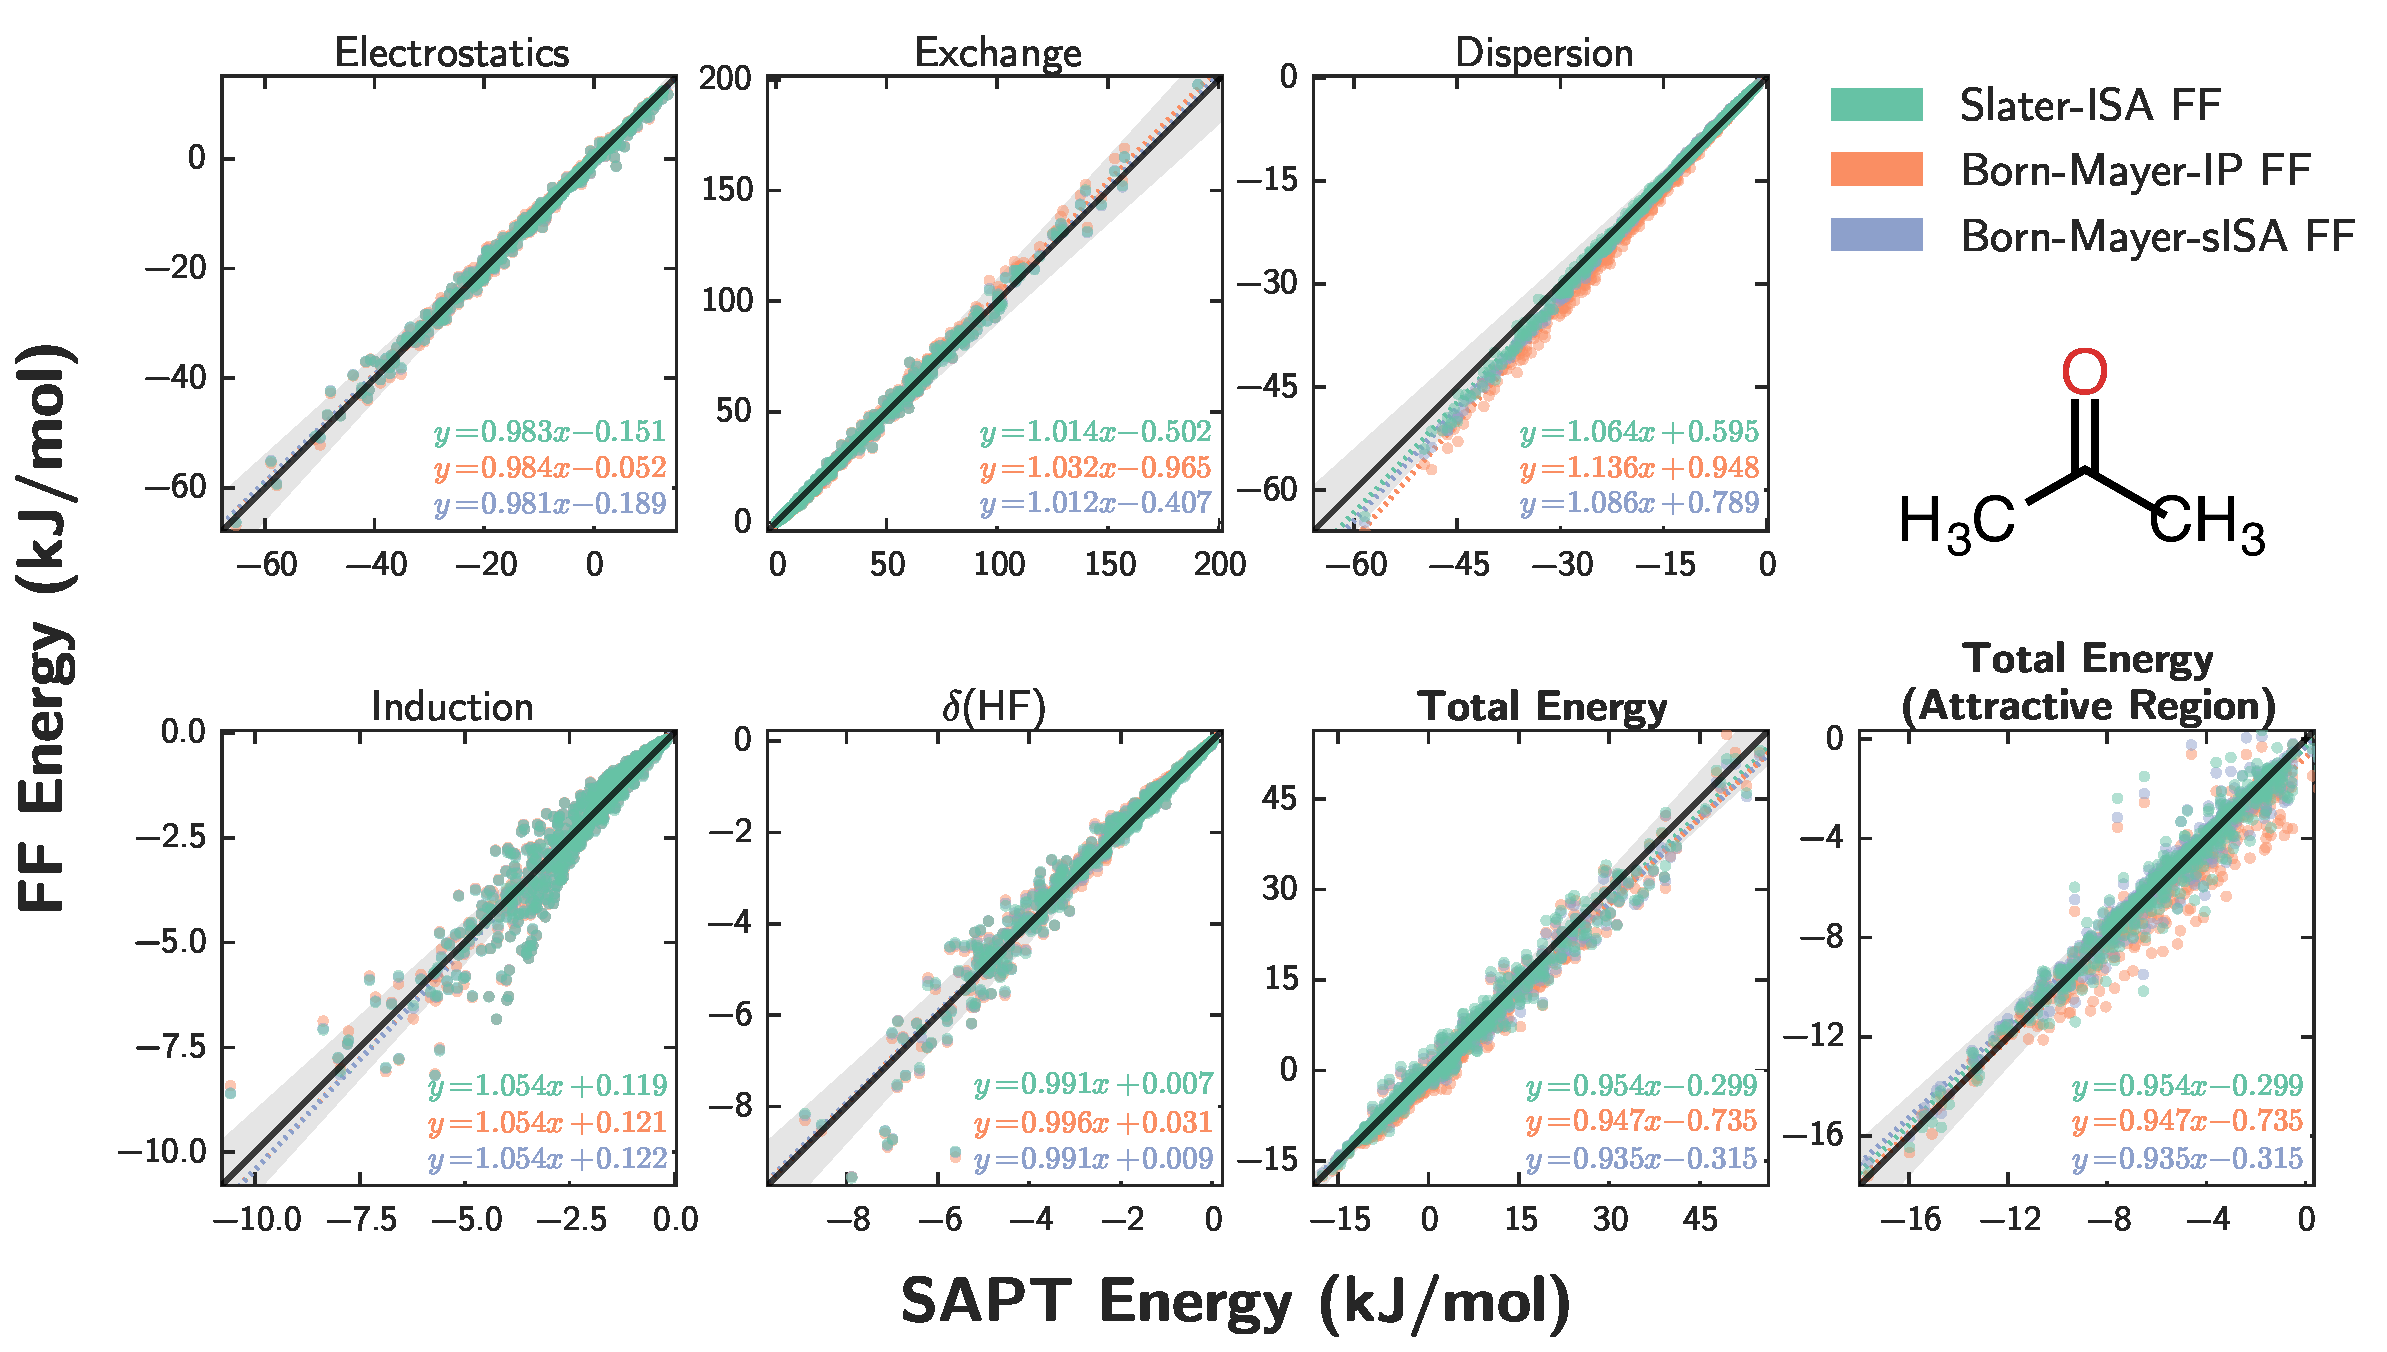
\includegraphics[width=0.9\textwidth]{isotropic/si/acetone_acetone_scatter.pdf}
    \end{subfigure}
    \begin{subfigure}{\textwidth}
        \caption{Ar Dimer}
        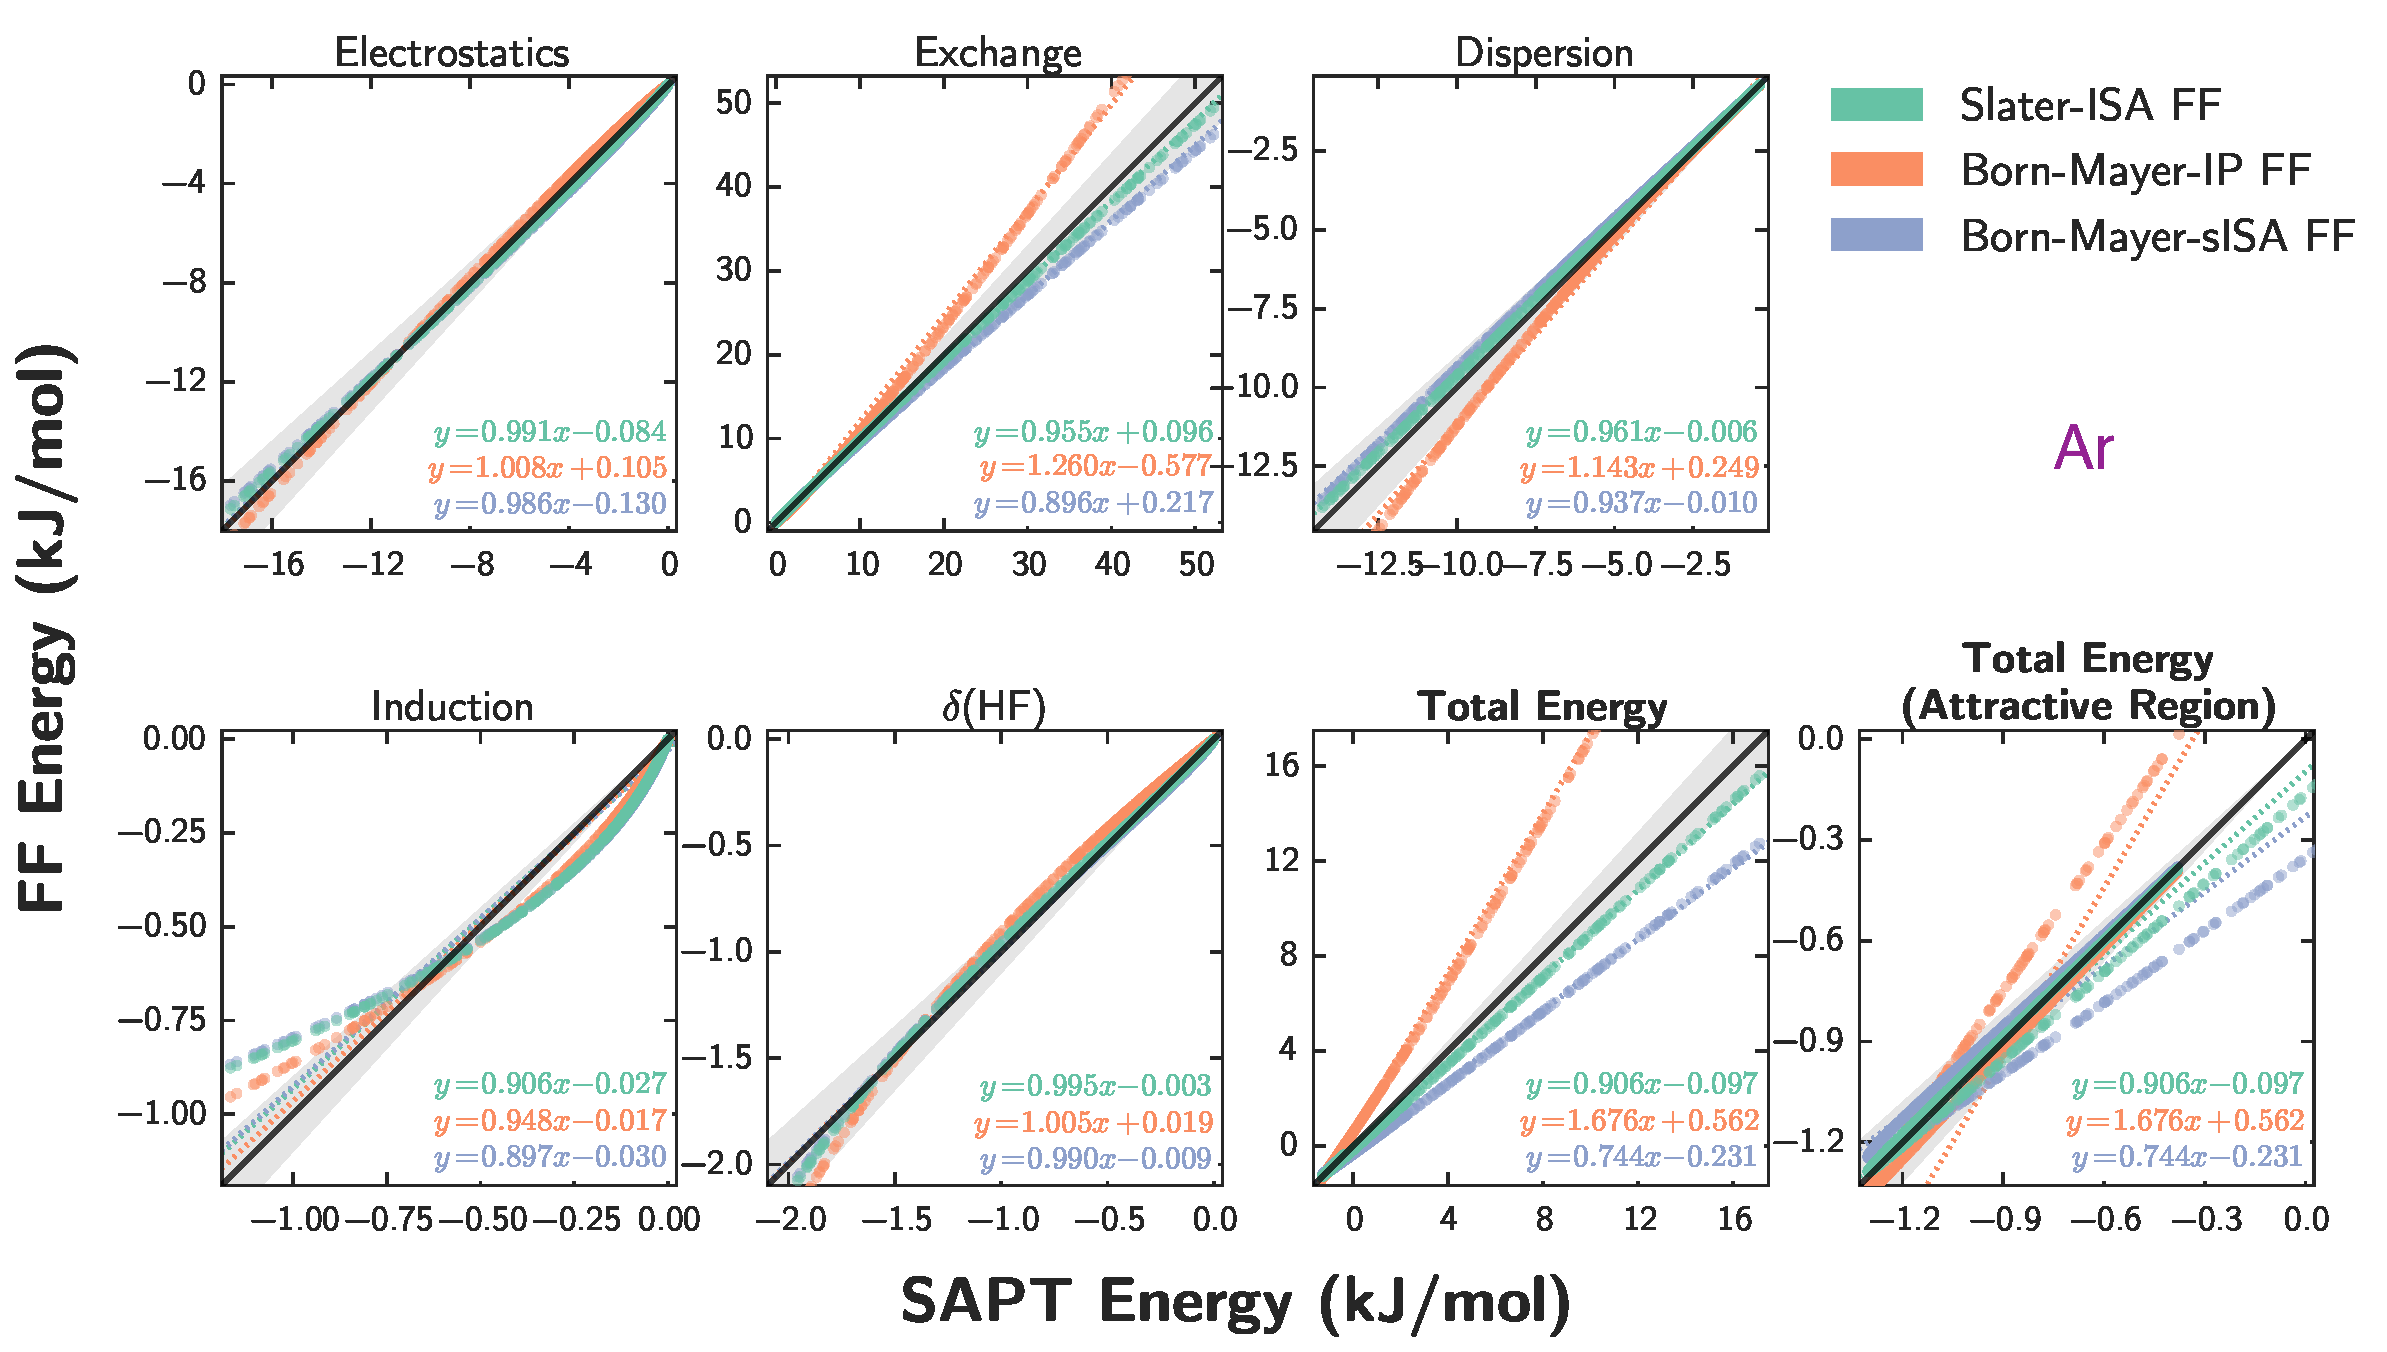
\includegraphics[width=0.9\textwidth]{isotropic/si/ar_ar_scatter.pdf}
    \end{subfigure}
    \end{figure}
    \begin{figure}
    \ContinuedFloat
    \begin{subfigure}{\textwidth}
        \caption{Chloromethane Dimer}
        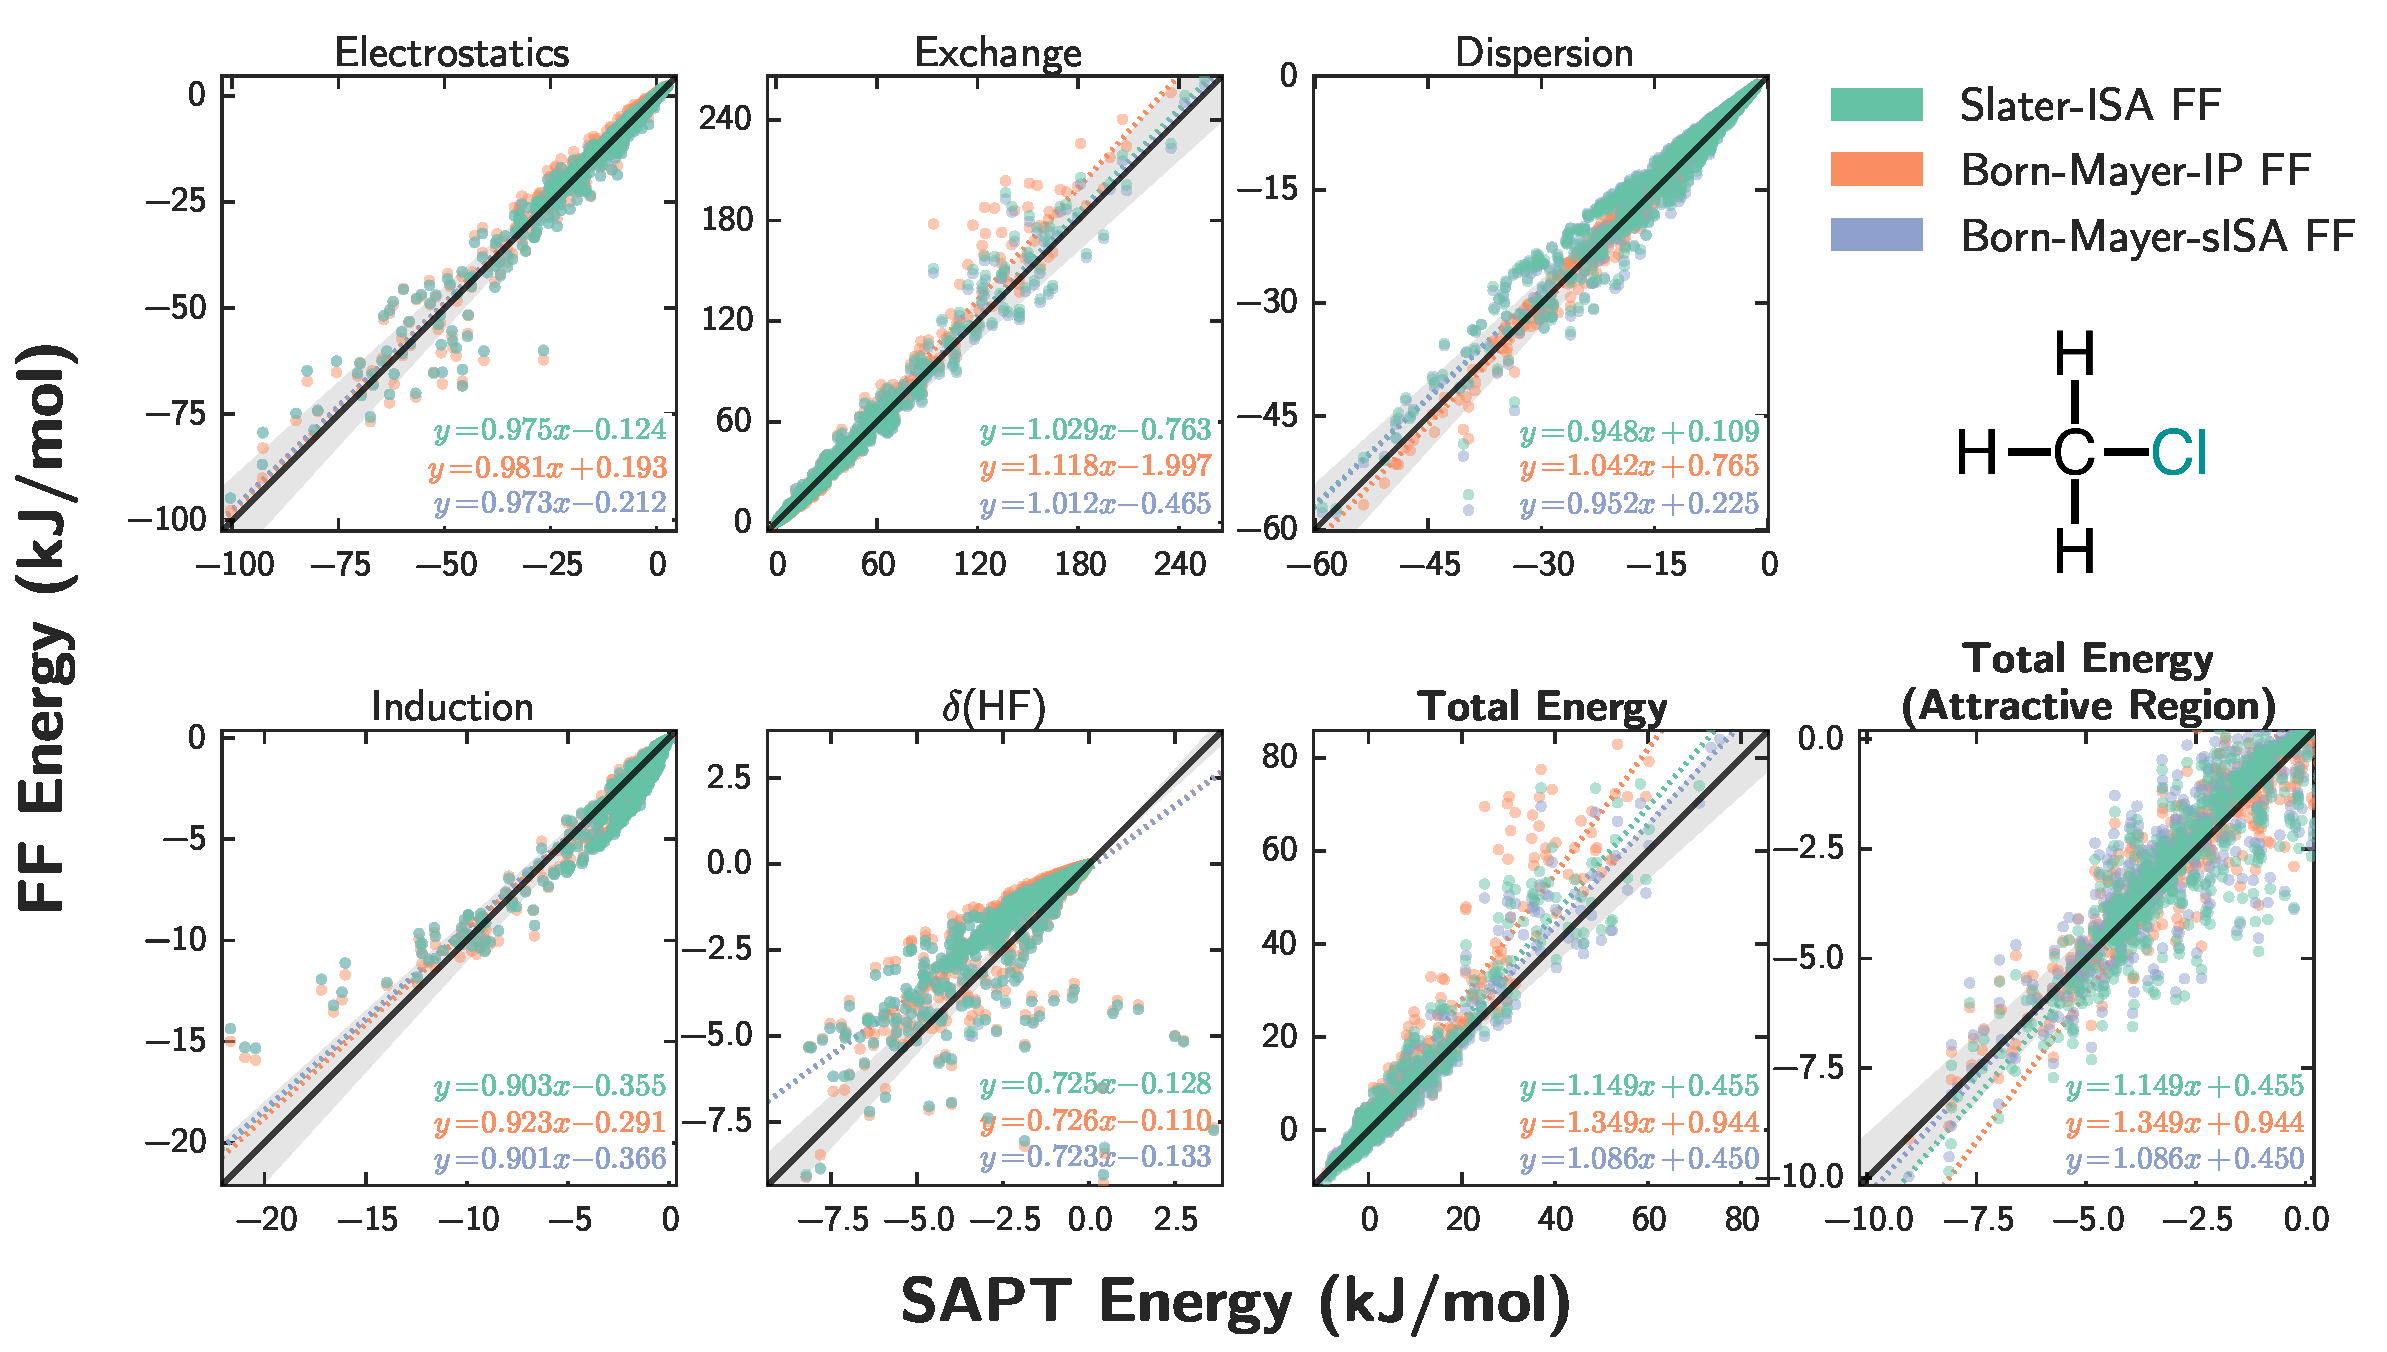
\includegraphics[width=0.9\textwidth]{isotropic/si/chloromethane_chloromethane_scatter.pdf}
    \end{subfigure}
    \begin{subfigure}{\textwidth}
        \caption{\co Dimer}
        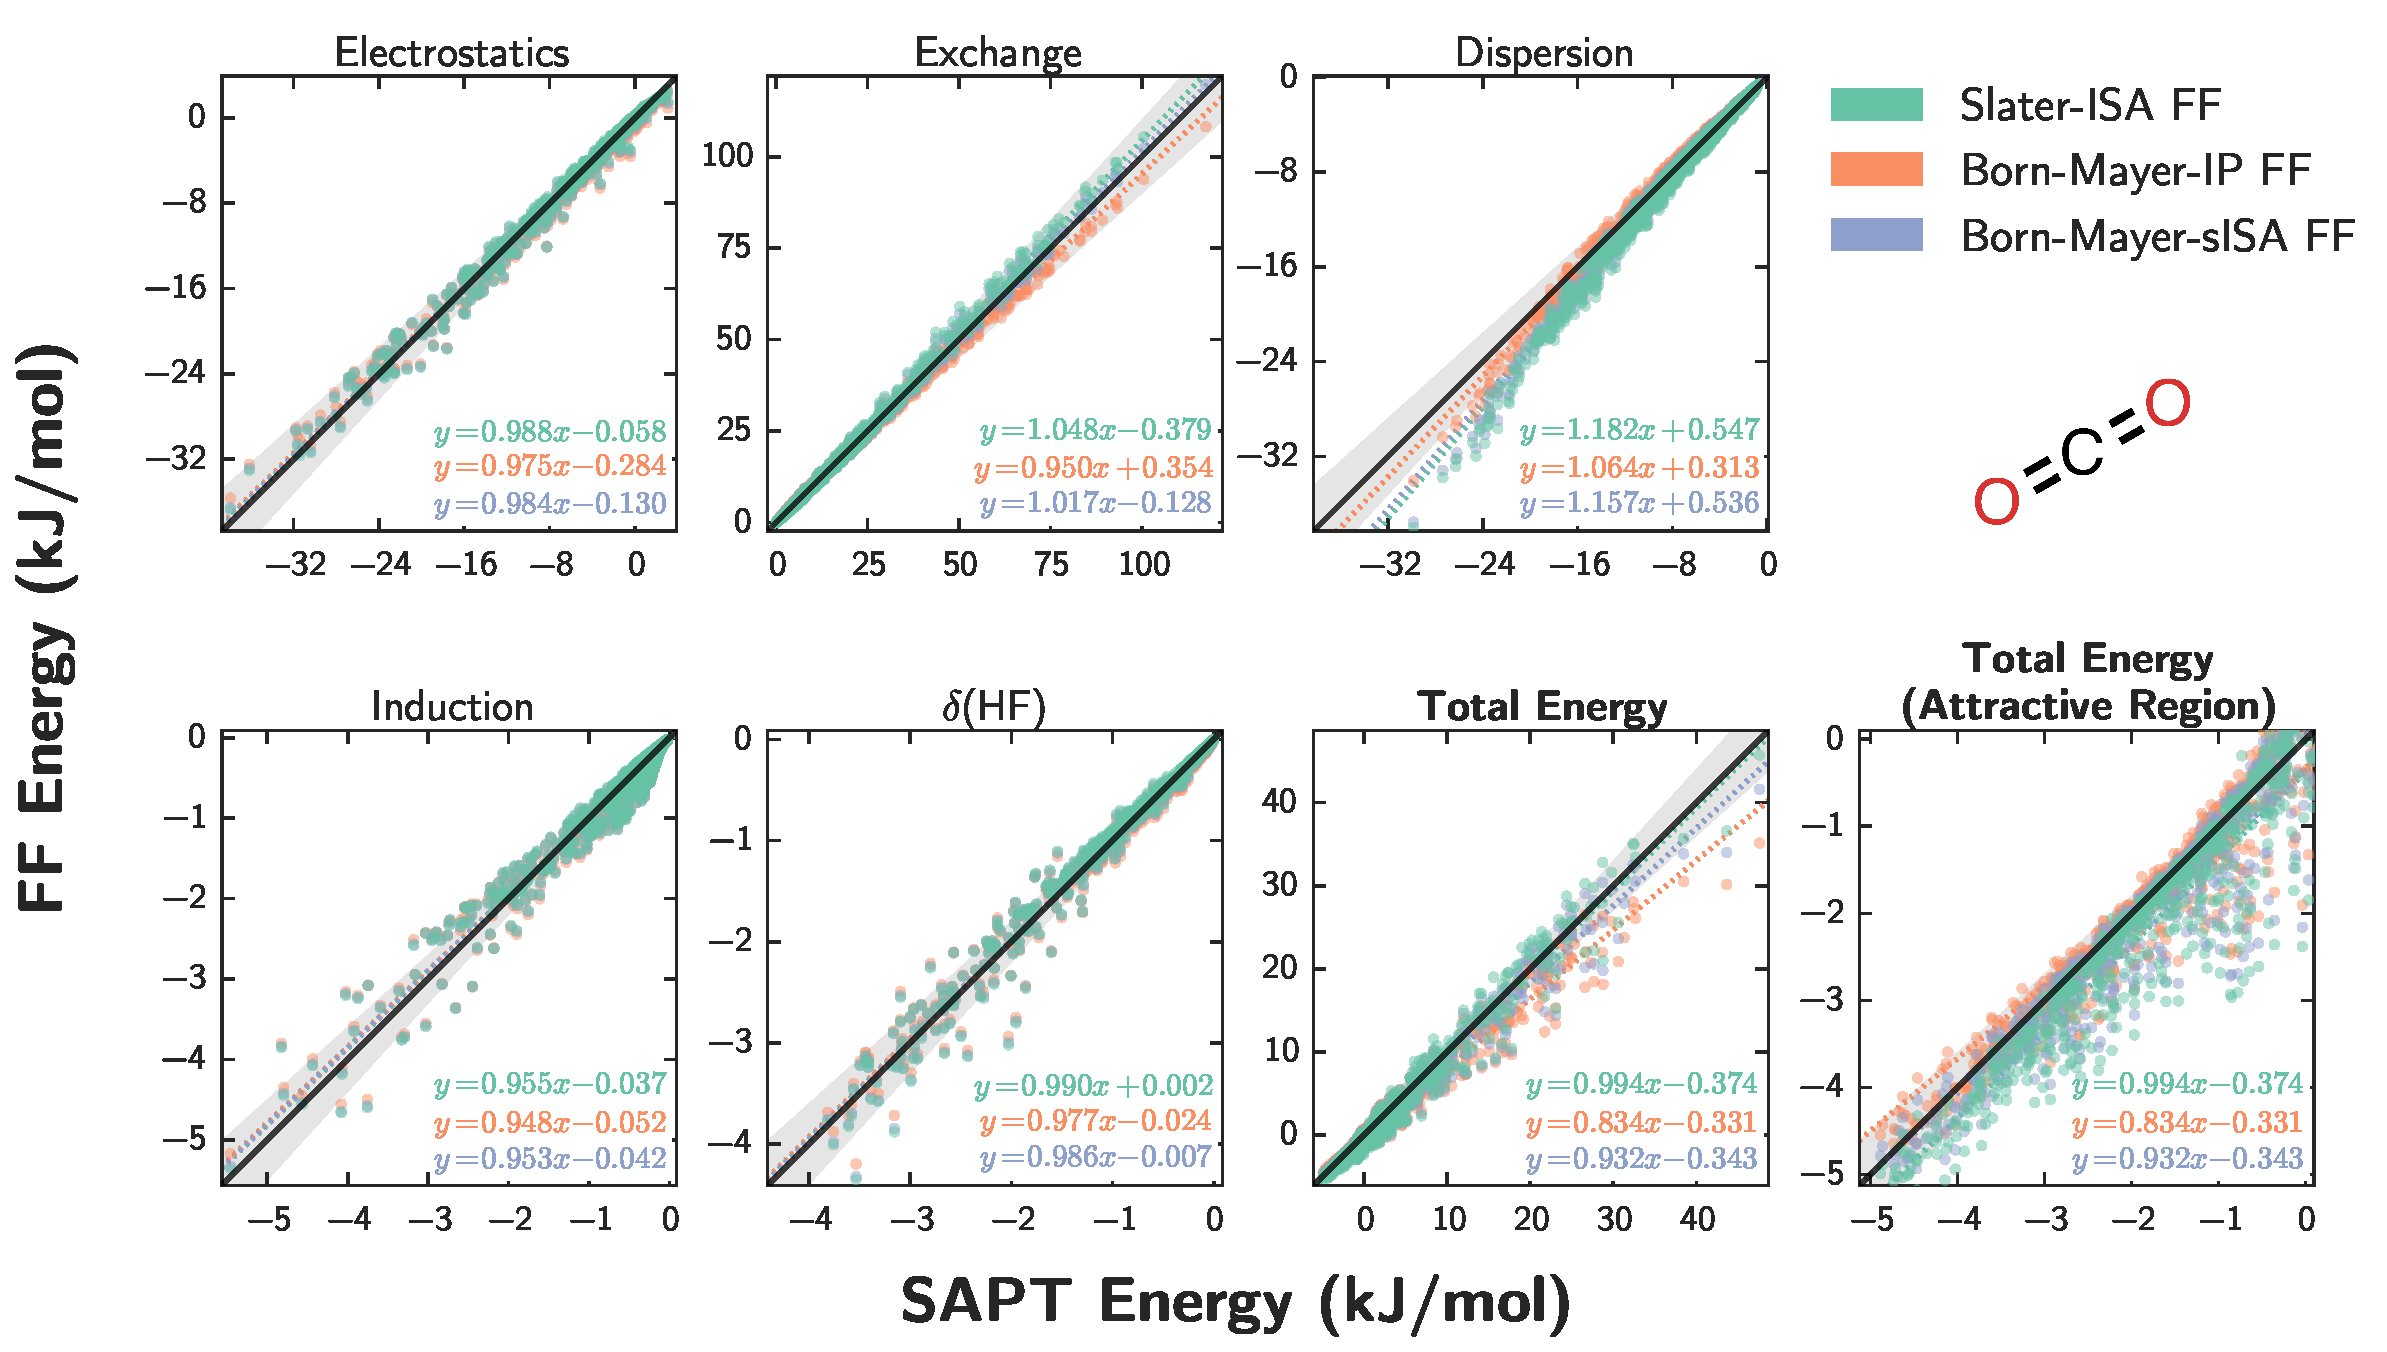
\includegraphics[width=0.9\textwidth]{isotropic/si/co2_co2_scatter.pdf}
    \end{subfigure}
    \end{figure}
    \begin{figure}
    \ContinuedFloat
    \begin{subfigure}{\textwidth}
        \caption{Dimethyl Ether Dimer}
        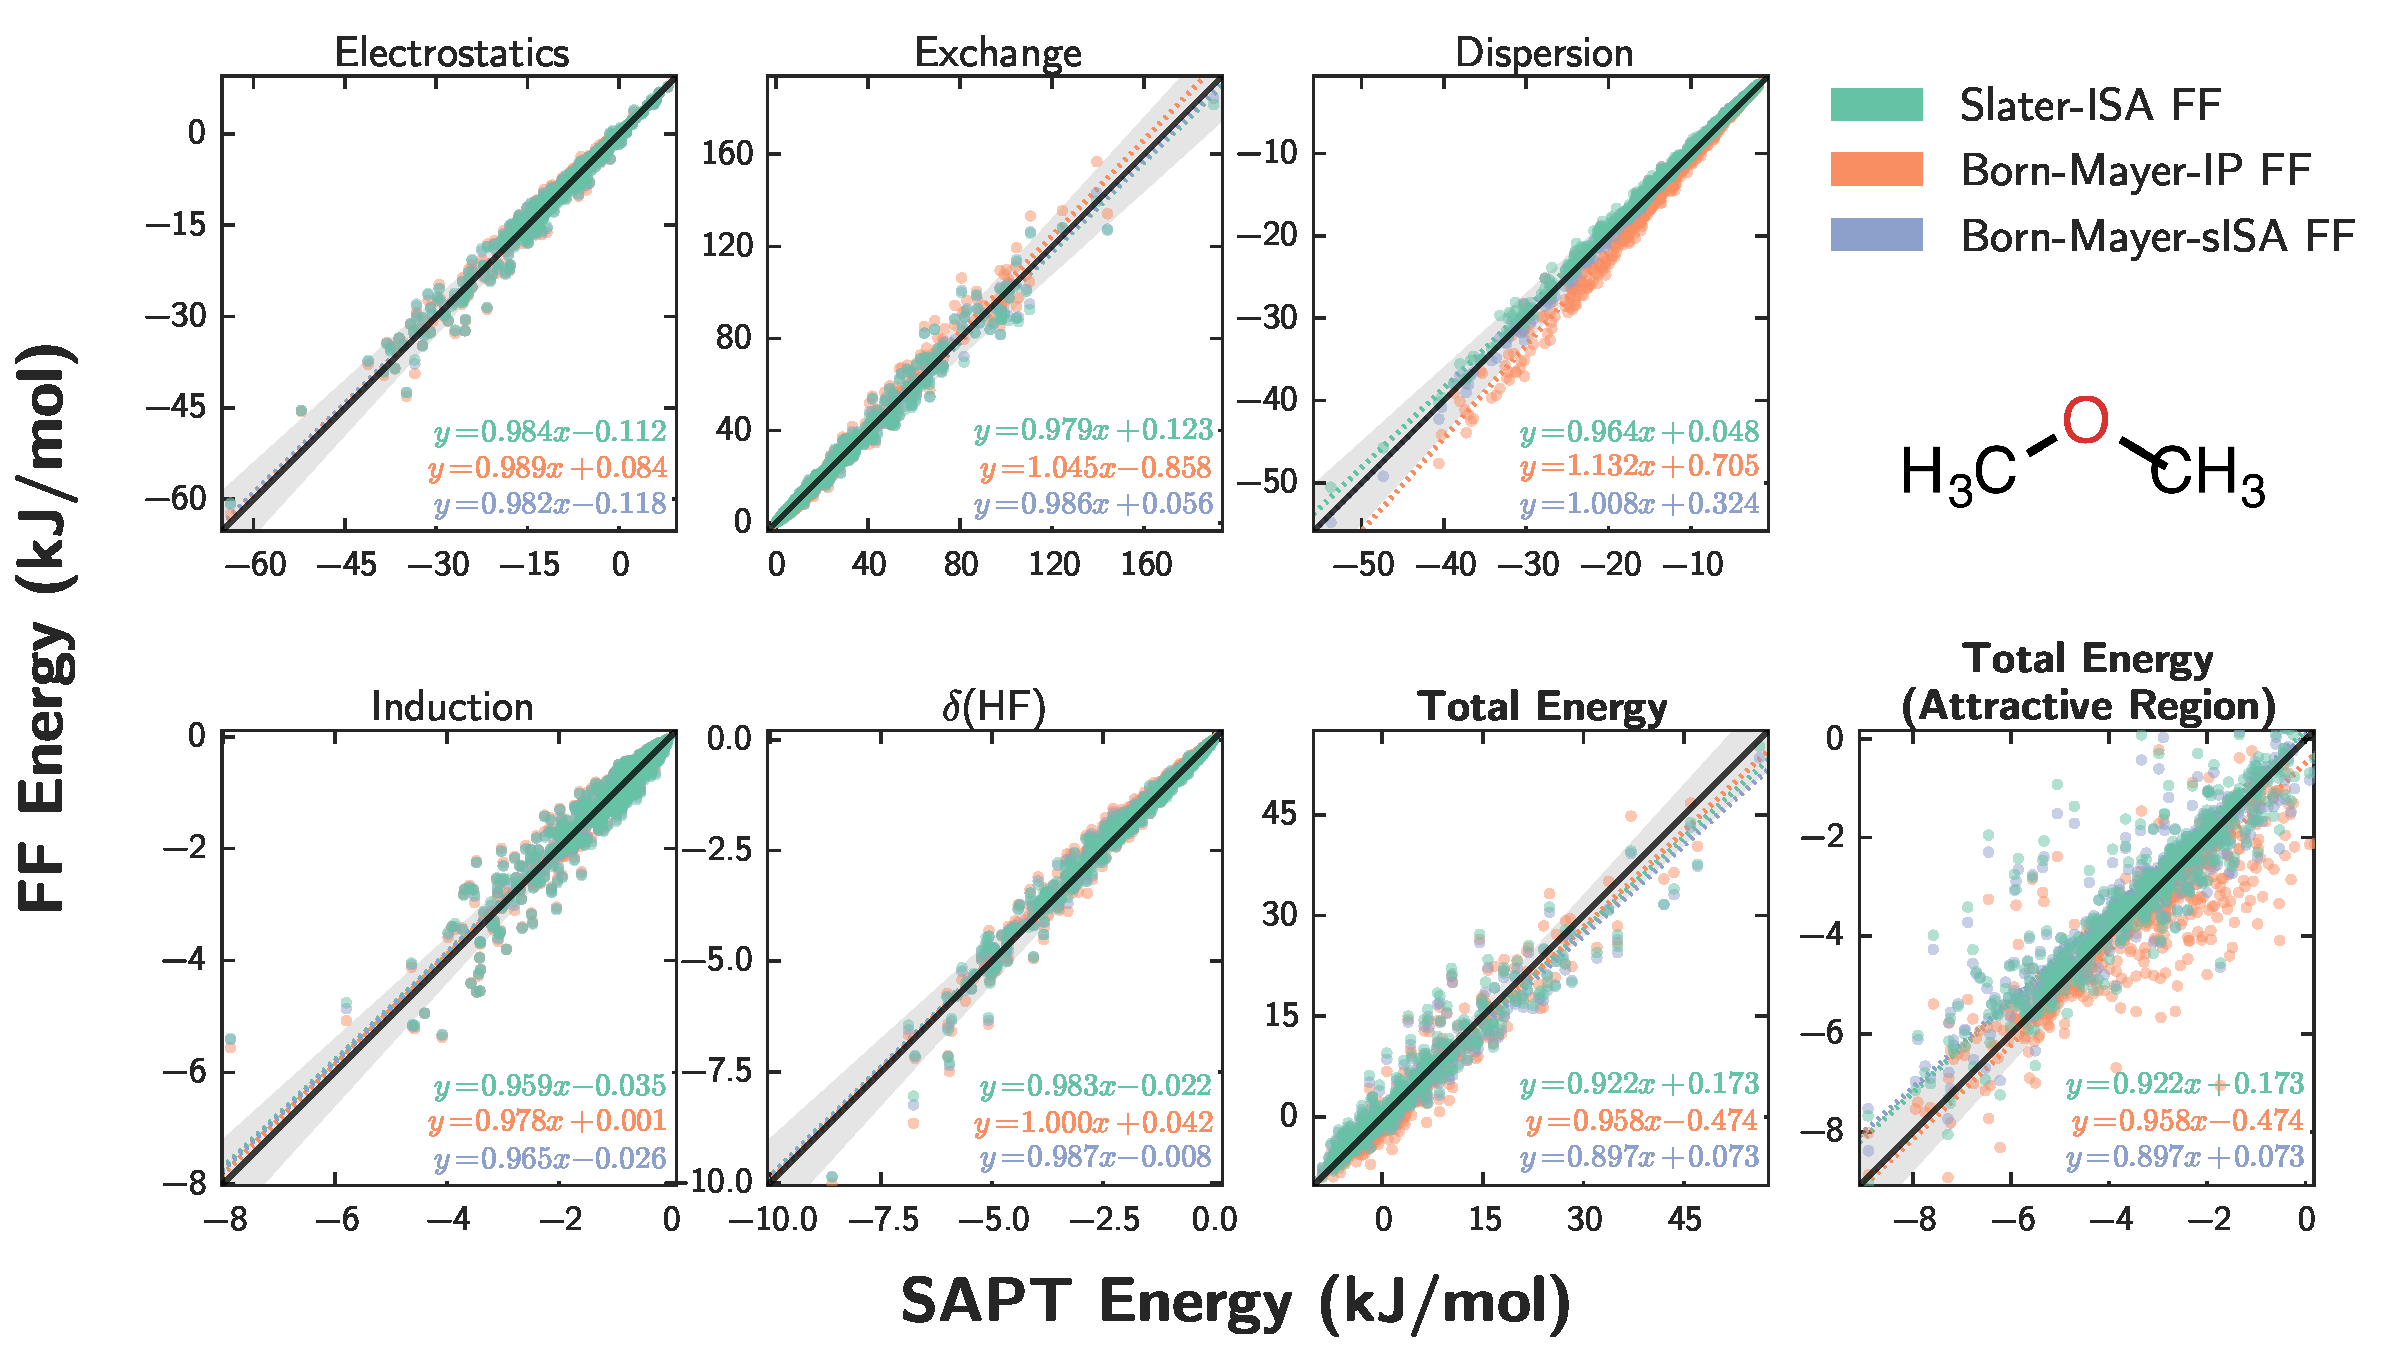
\includegraphics[width=0.9\textwidth]{isotropic/si/dimethyl_ether_dimethyl_ether_scatter.pdf}
    \end{subfigure}
    \begin{subfigure}{\textwidth}
        \caption{Ethane Dimer}
        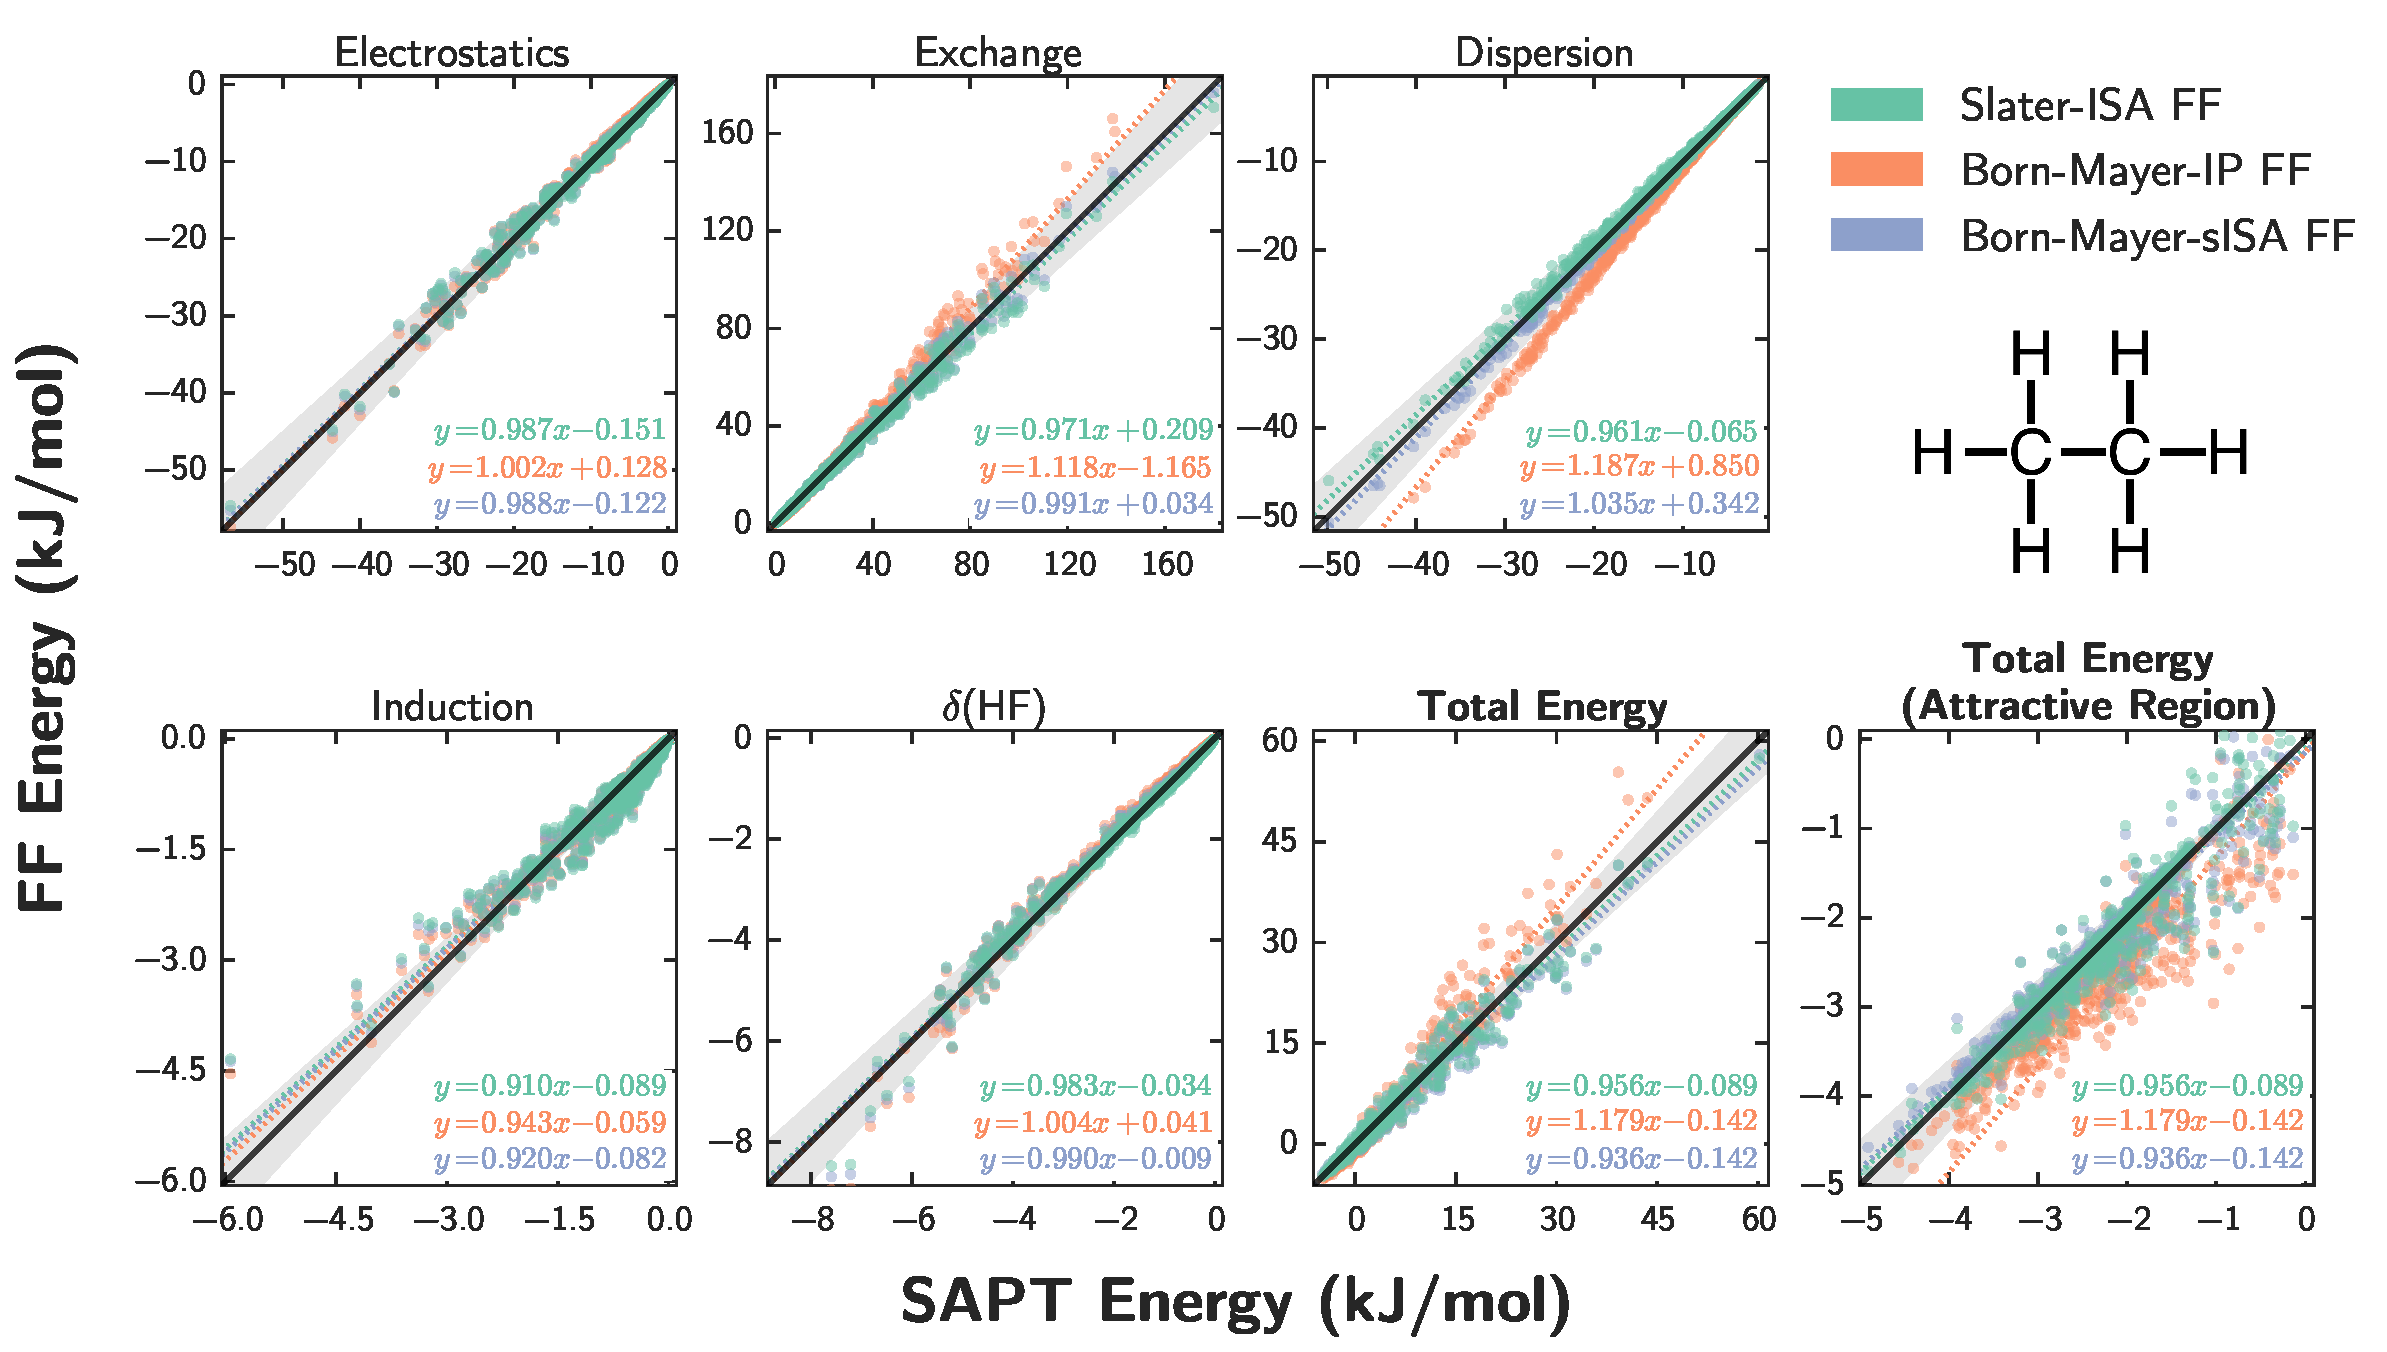
\includegraphics[width=0.9\textwidth]{isotropic/si/ethane_ethane_scatter.pdf}
    \end{subfigure}
    \end{figure}
    \begin{figure}
    \ContinuedFloat
    \begin{subfigure}{\textwidth}
        \caption{Ethanol Dimer}
        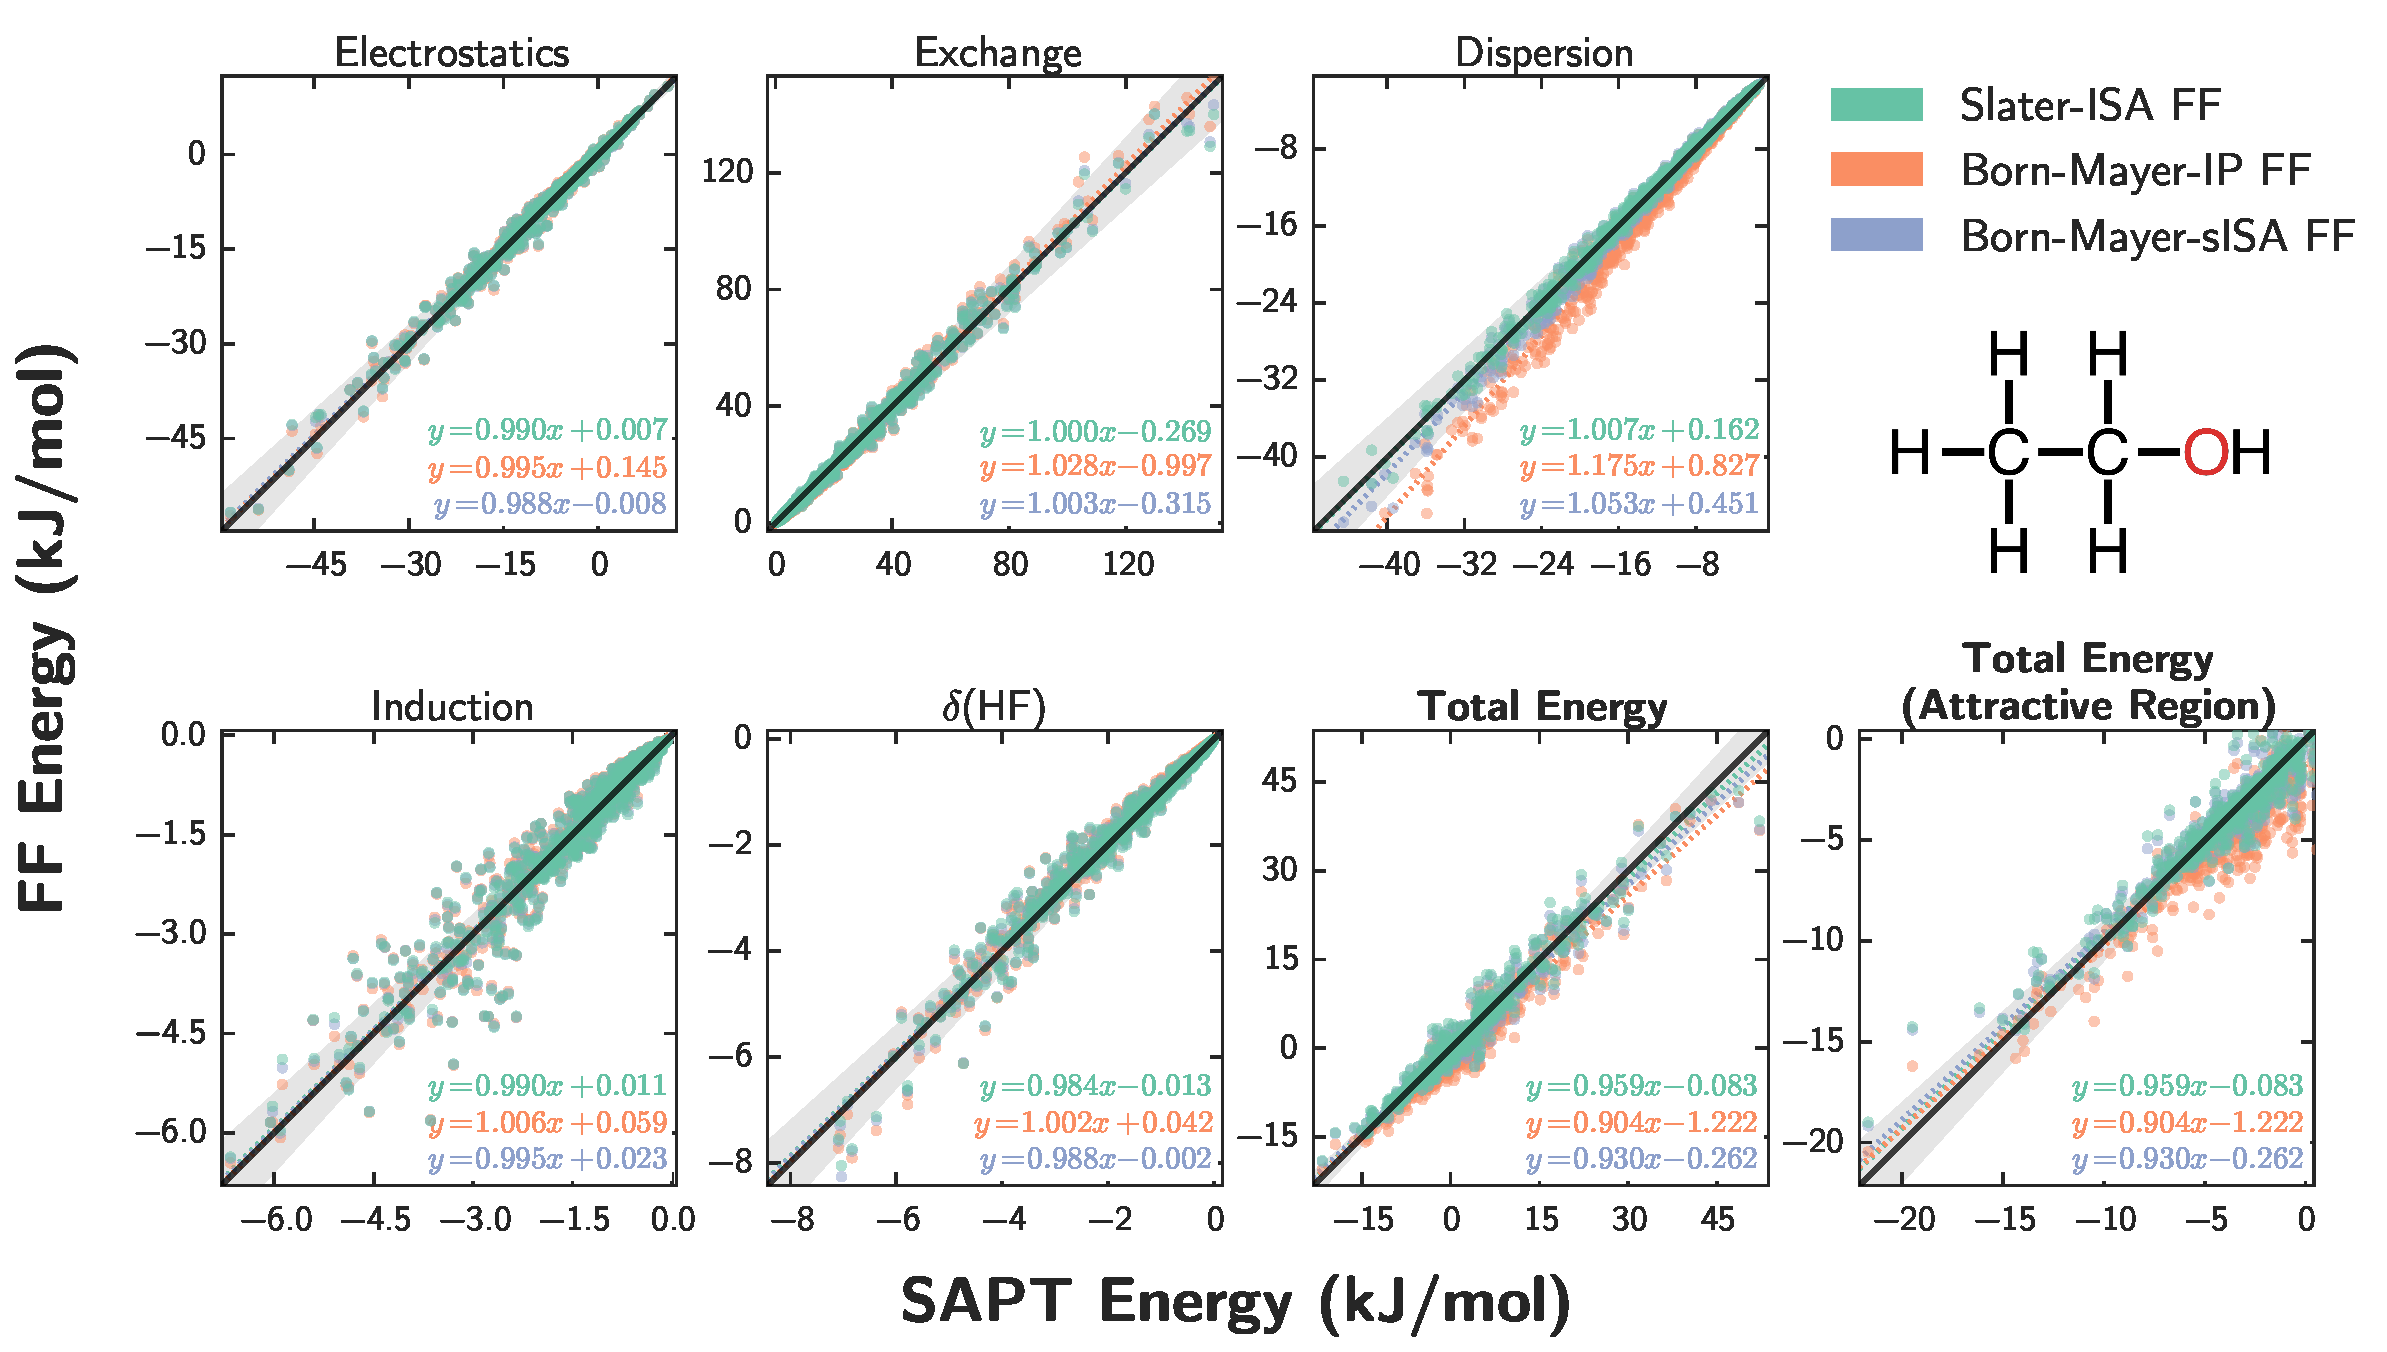
\includegraphics[width=0.9\textwidth]{isotropic/si/ethanol_ethanol_scatter.pdf}
    \end{subfigure}
    \begin{subfigure}{\textwidth}
        \caption{Ethene Dimer}
        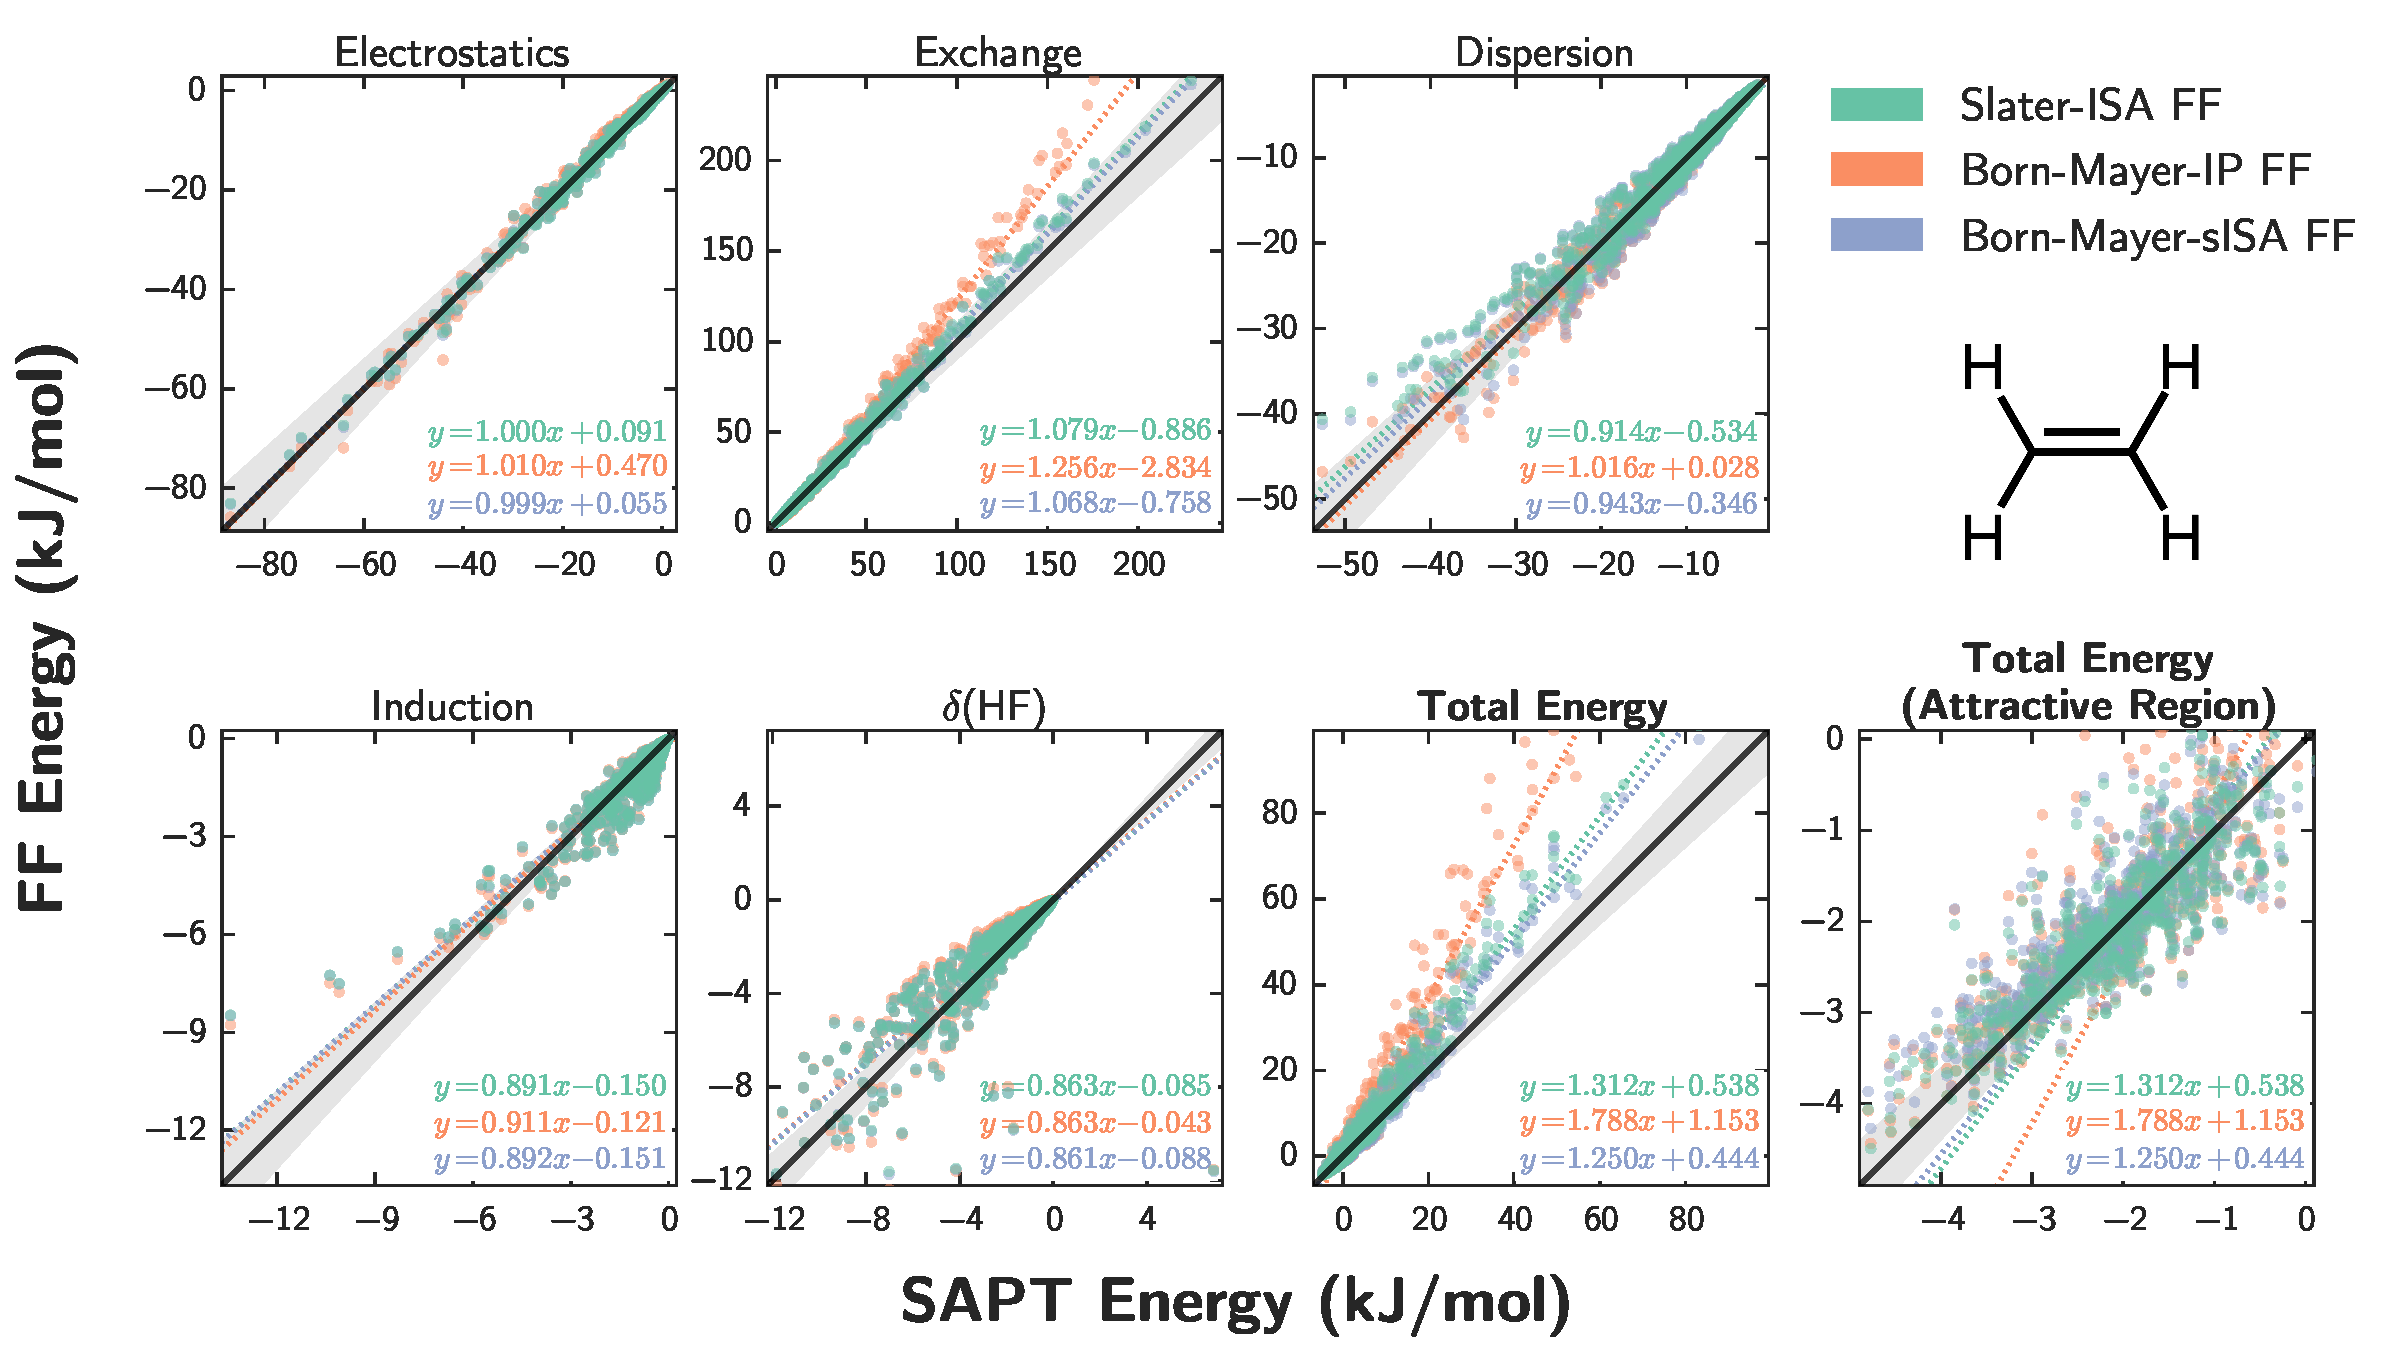
\includegraphics[width=0.9\textwidth]{isotropic/si/ethene_ethene_scatter.pdf}
    \end{subfigure}
    \end{figure}
    \begin{figure}
    \ContinuedFloat
    \begin{subfigure}{\textwidth}
        \caption{\ho Dimer}
        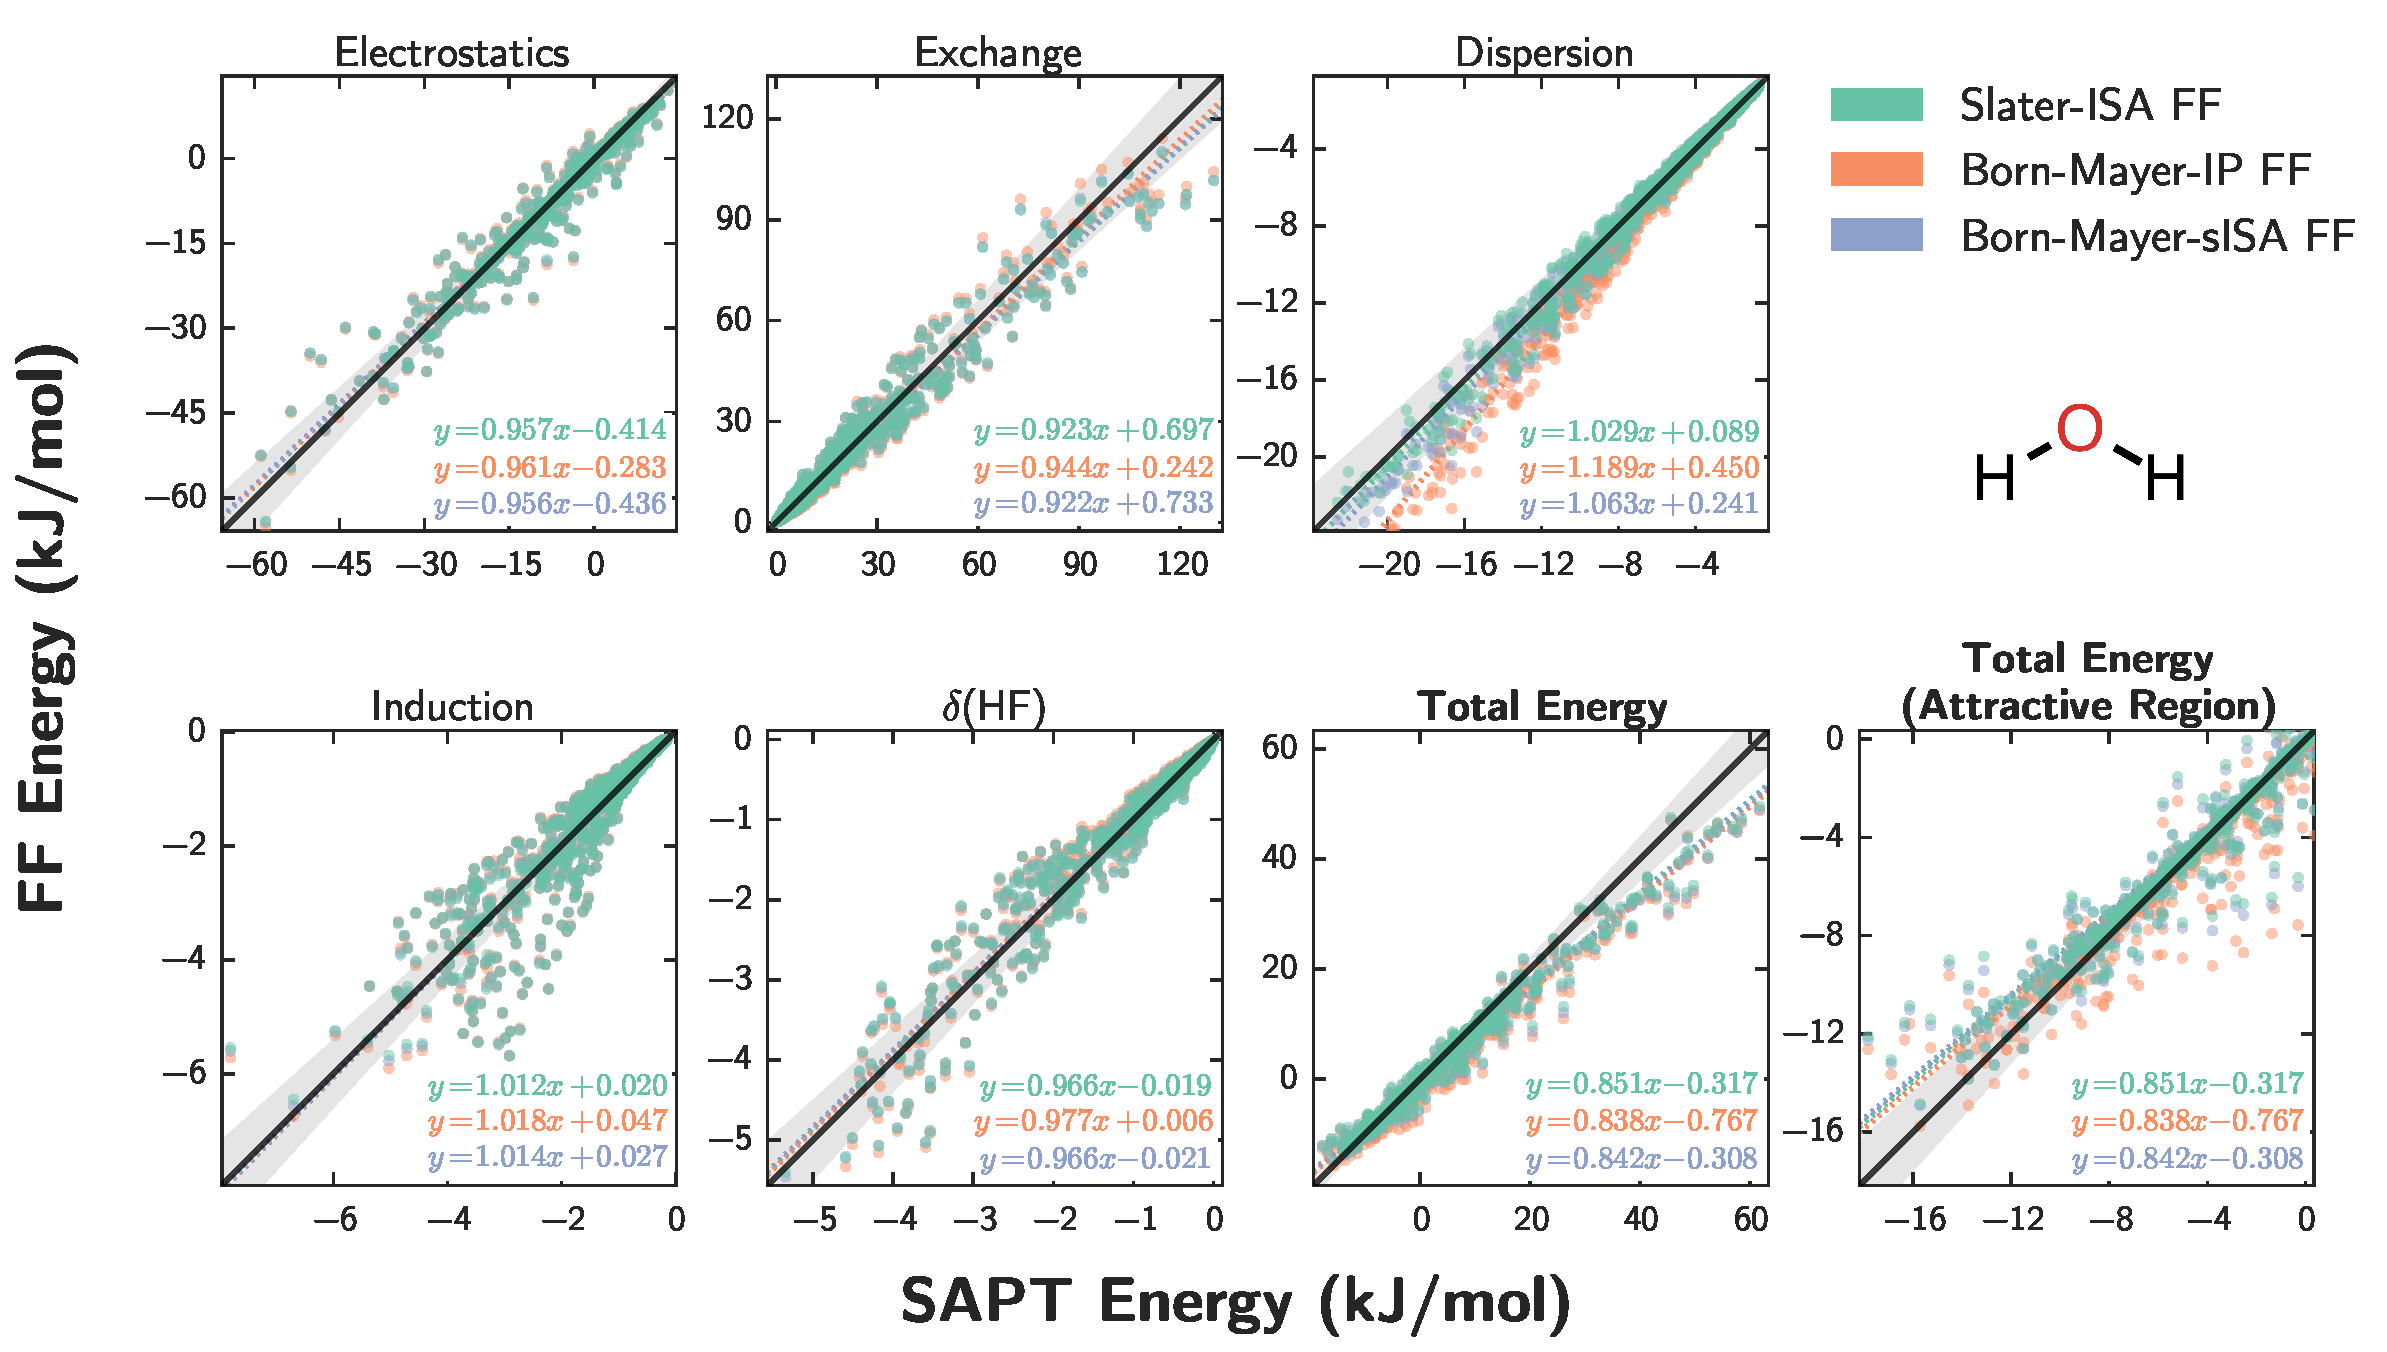
\includegraphics[width=0.9\textwidth]{isotropic/si/h2o_h2o_scatter.pdf}
    \end{subfigure}
    \begin{subfigure}{\textwidth}
        \caption{Methane Dimer}
        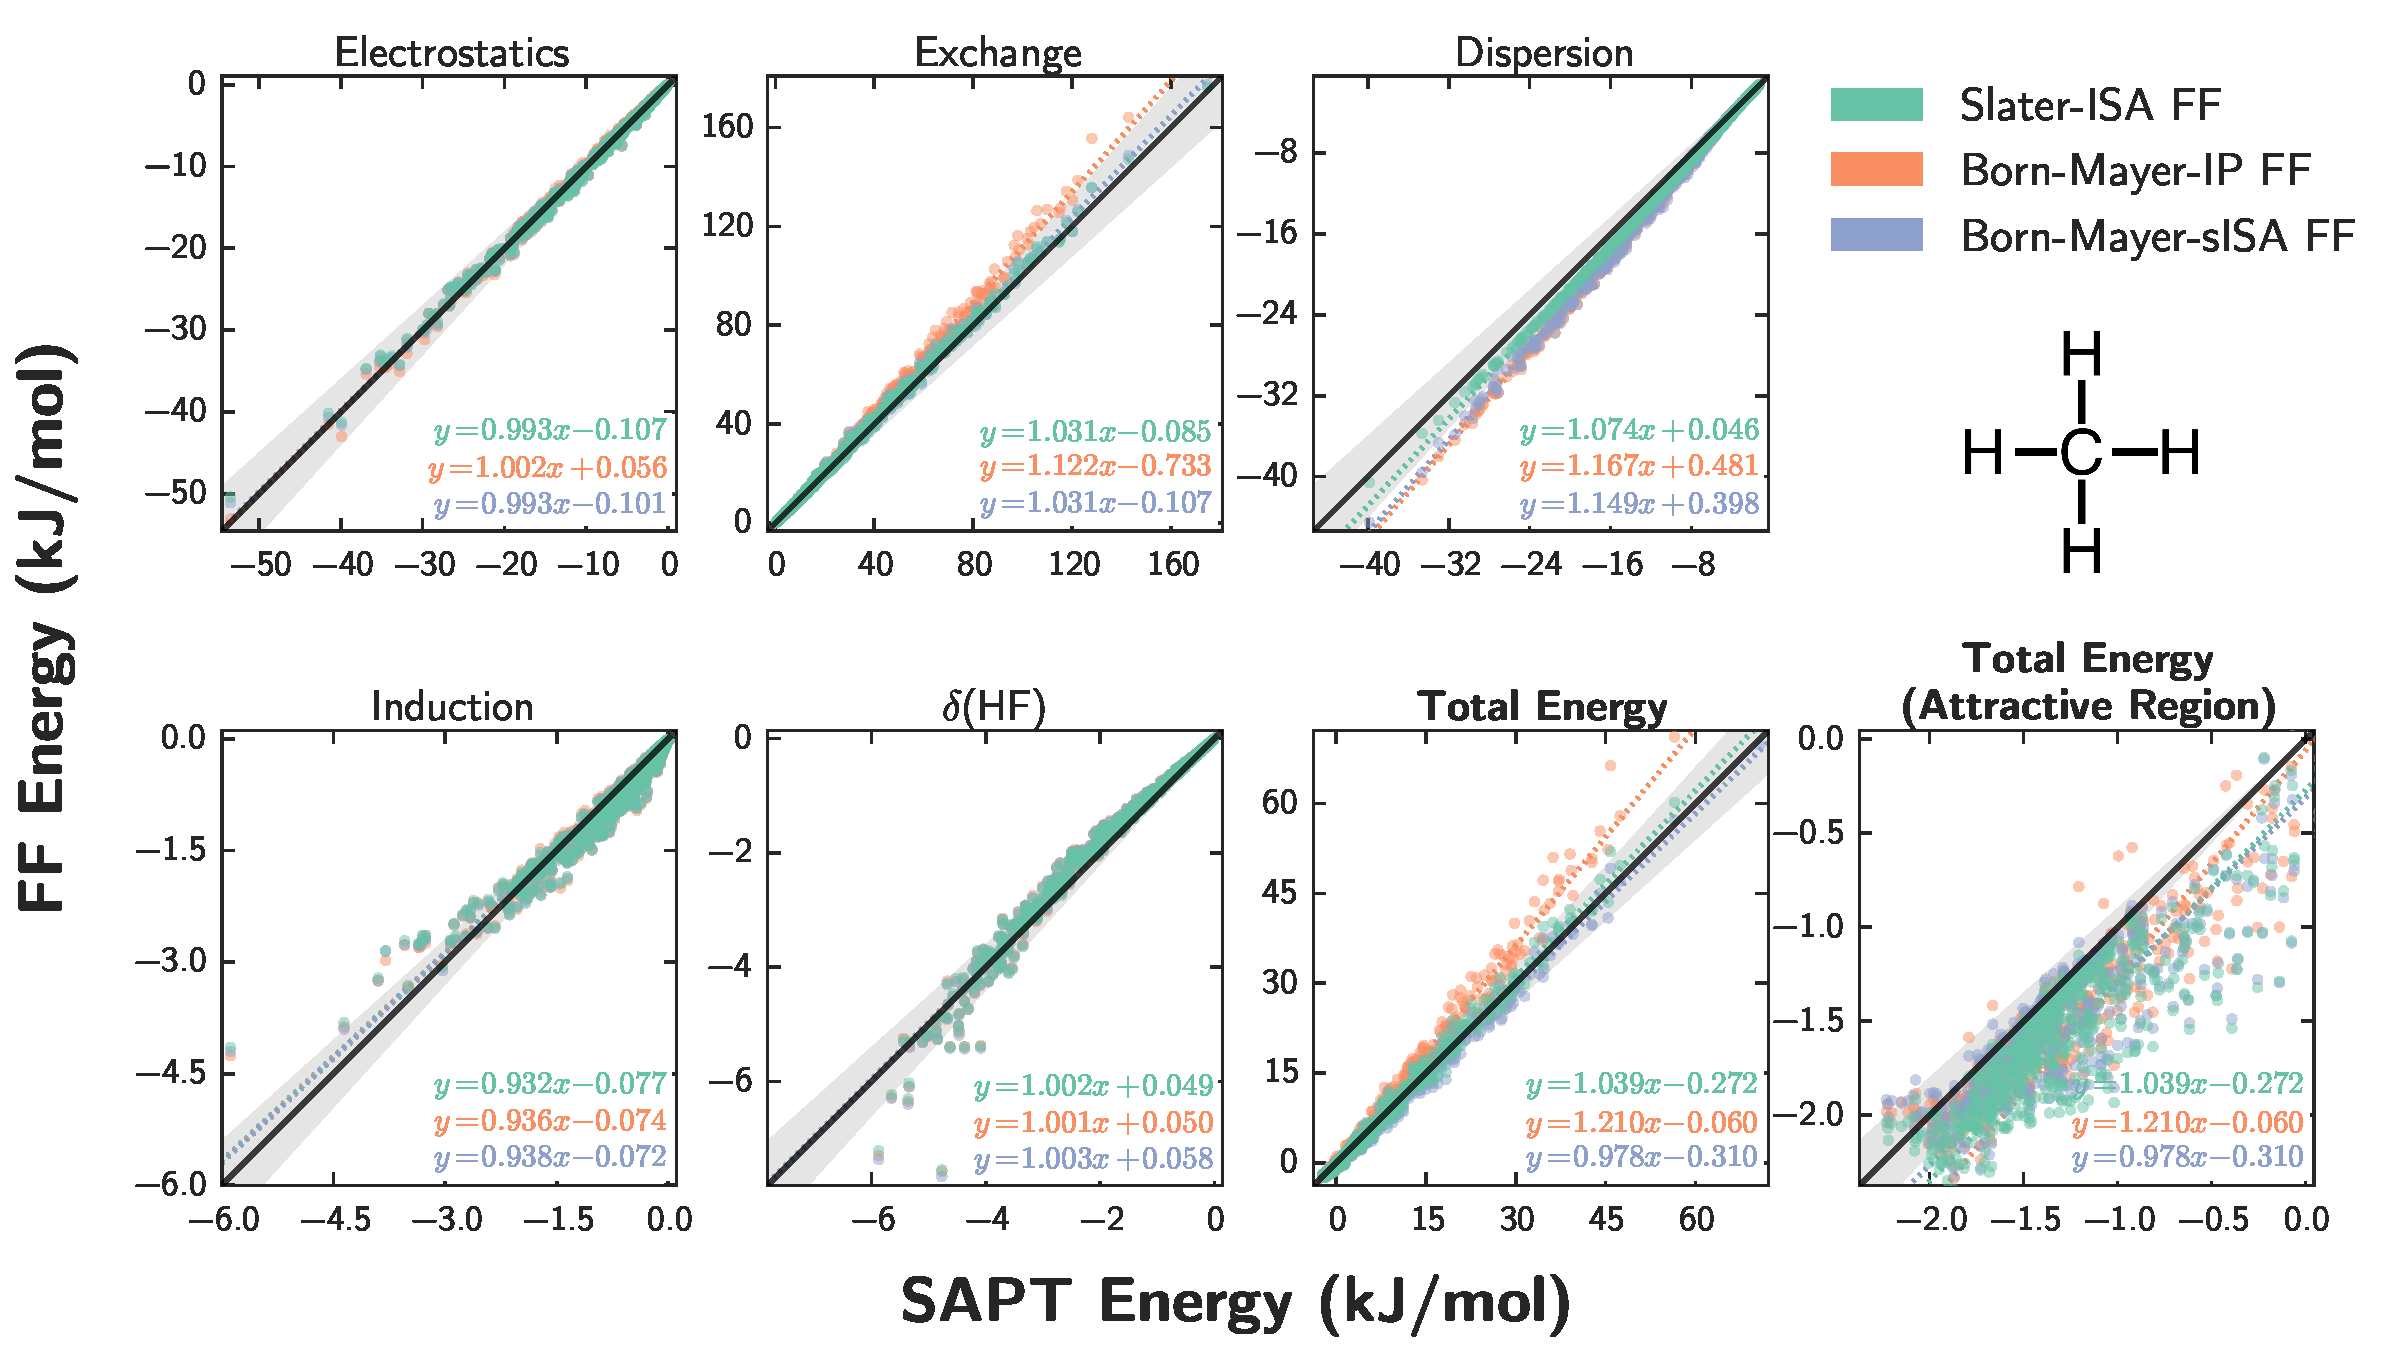
\includegraphics[width=0.9\textwidth]{isotropic/si/methane_methane_scatter.pdf}
    \end{subfigure}
    \end{figure}
    \begin{figure}
    \ContinuedFloat
    \begin{subfigure}{\textwidth}
        \caption{Methanol Dimer}
        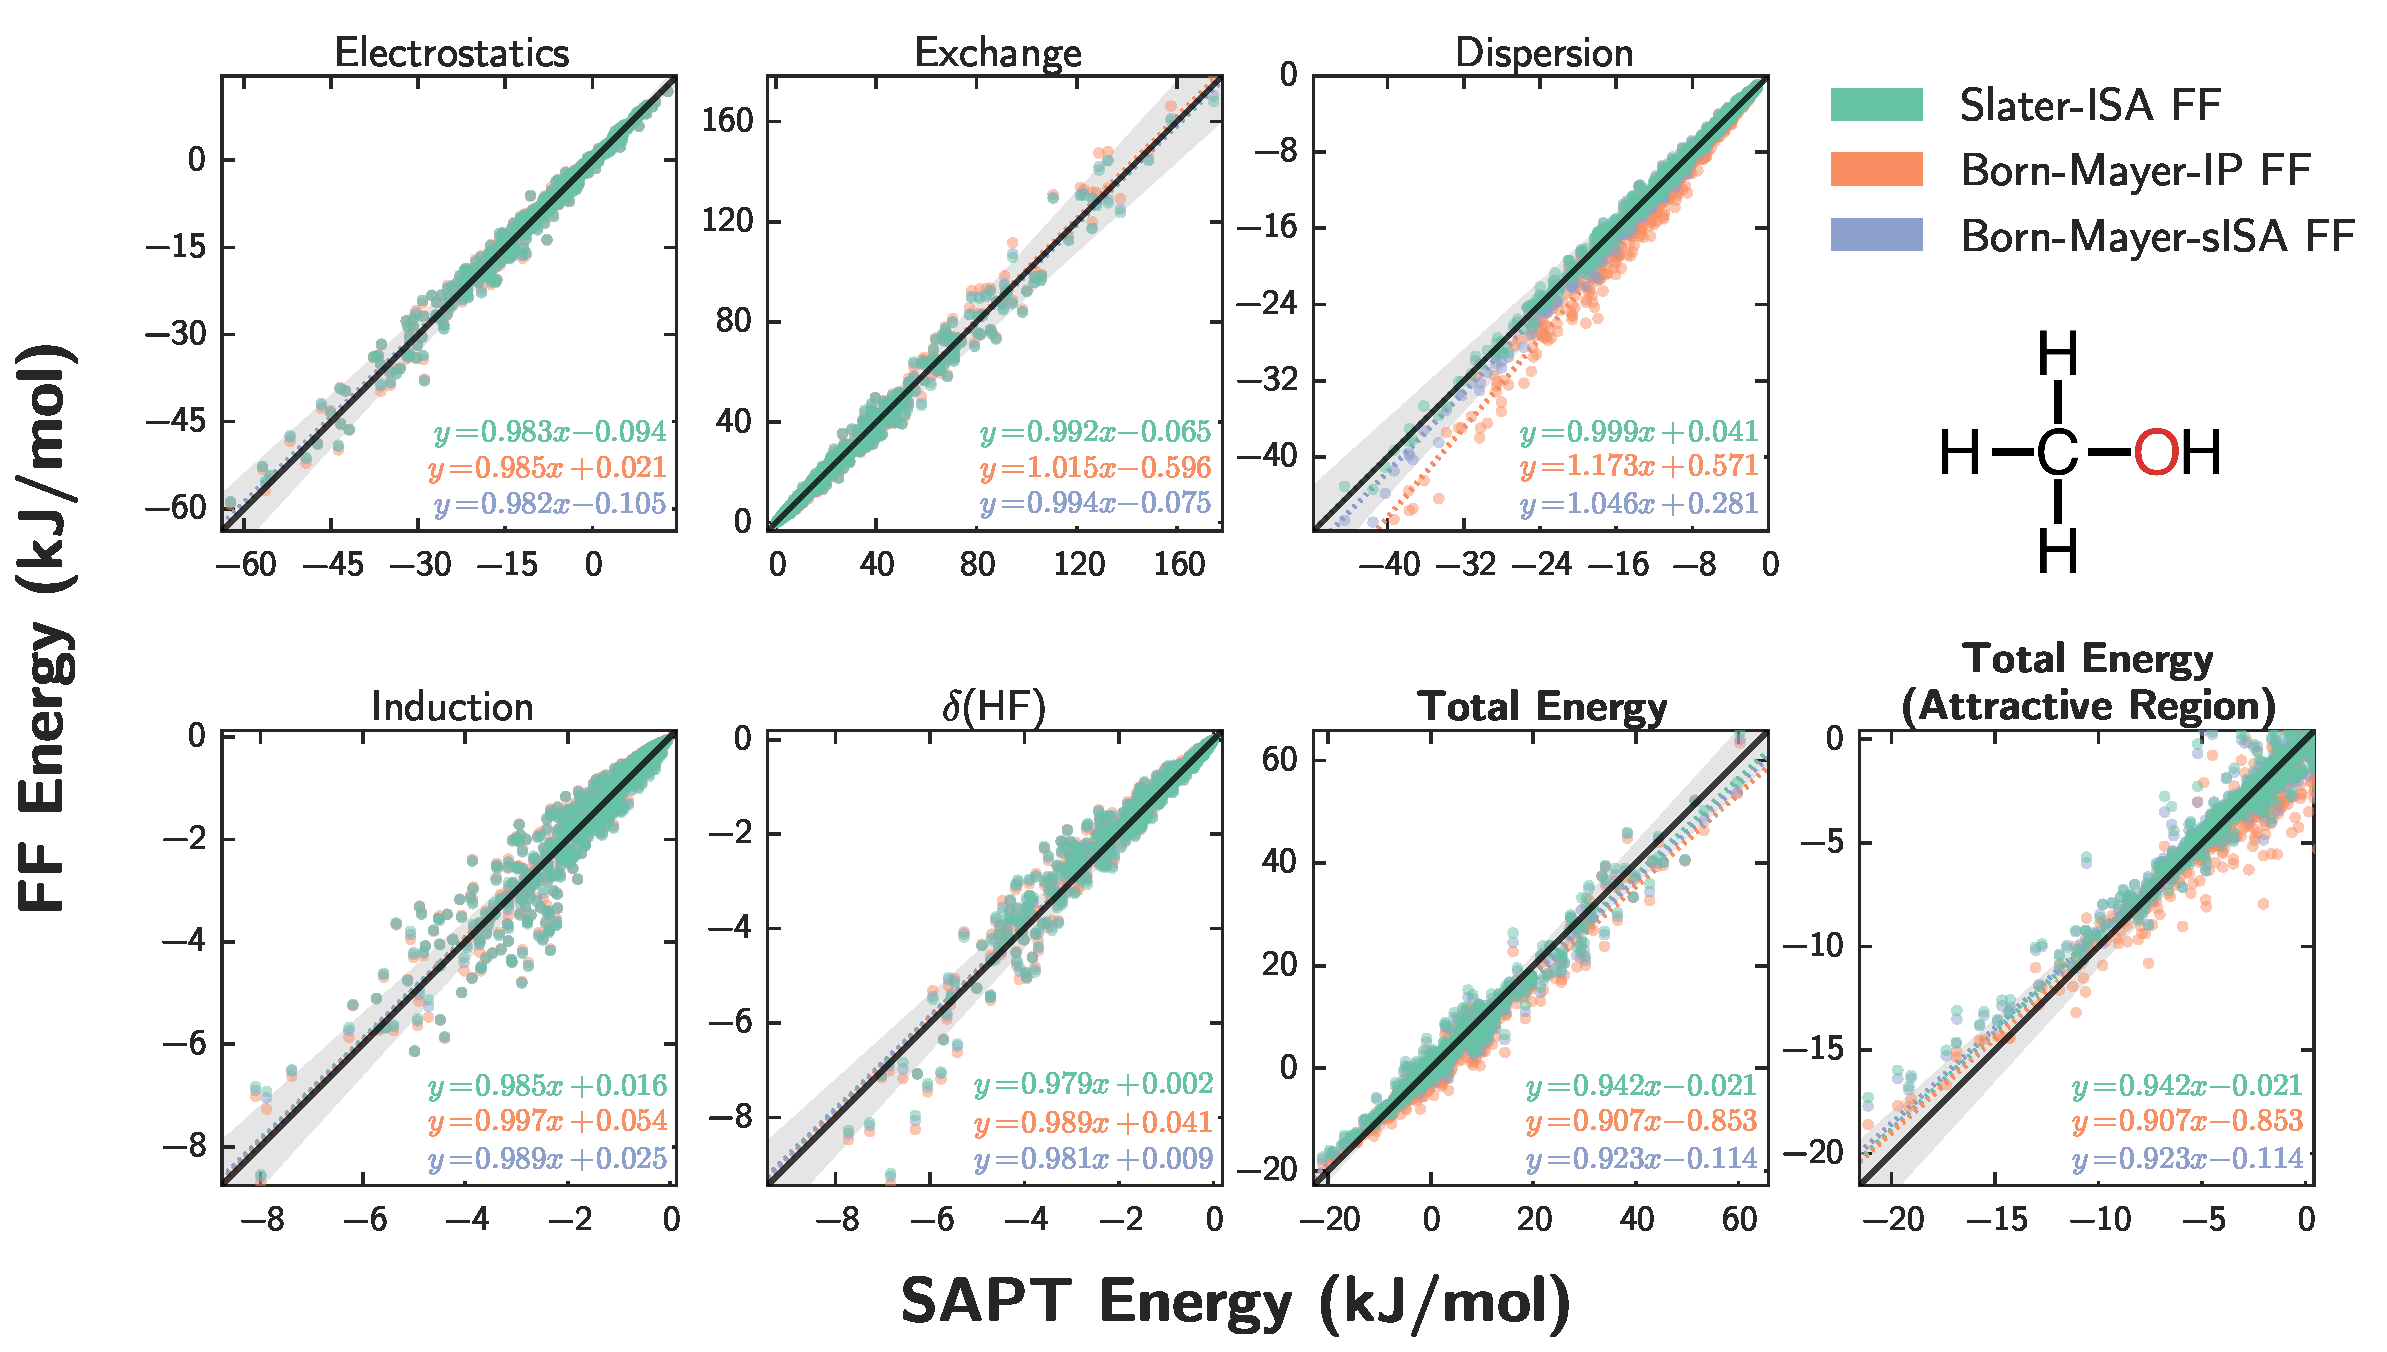
\includegraphics[width=0.9\textwidth]{isotropic/si/methanol_methanol_scatter.pdf}
    \end{subfigure}
    \begin{subfigure}{\textwidth}
        \caption{Methyl Amine Dimer}
        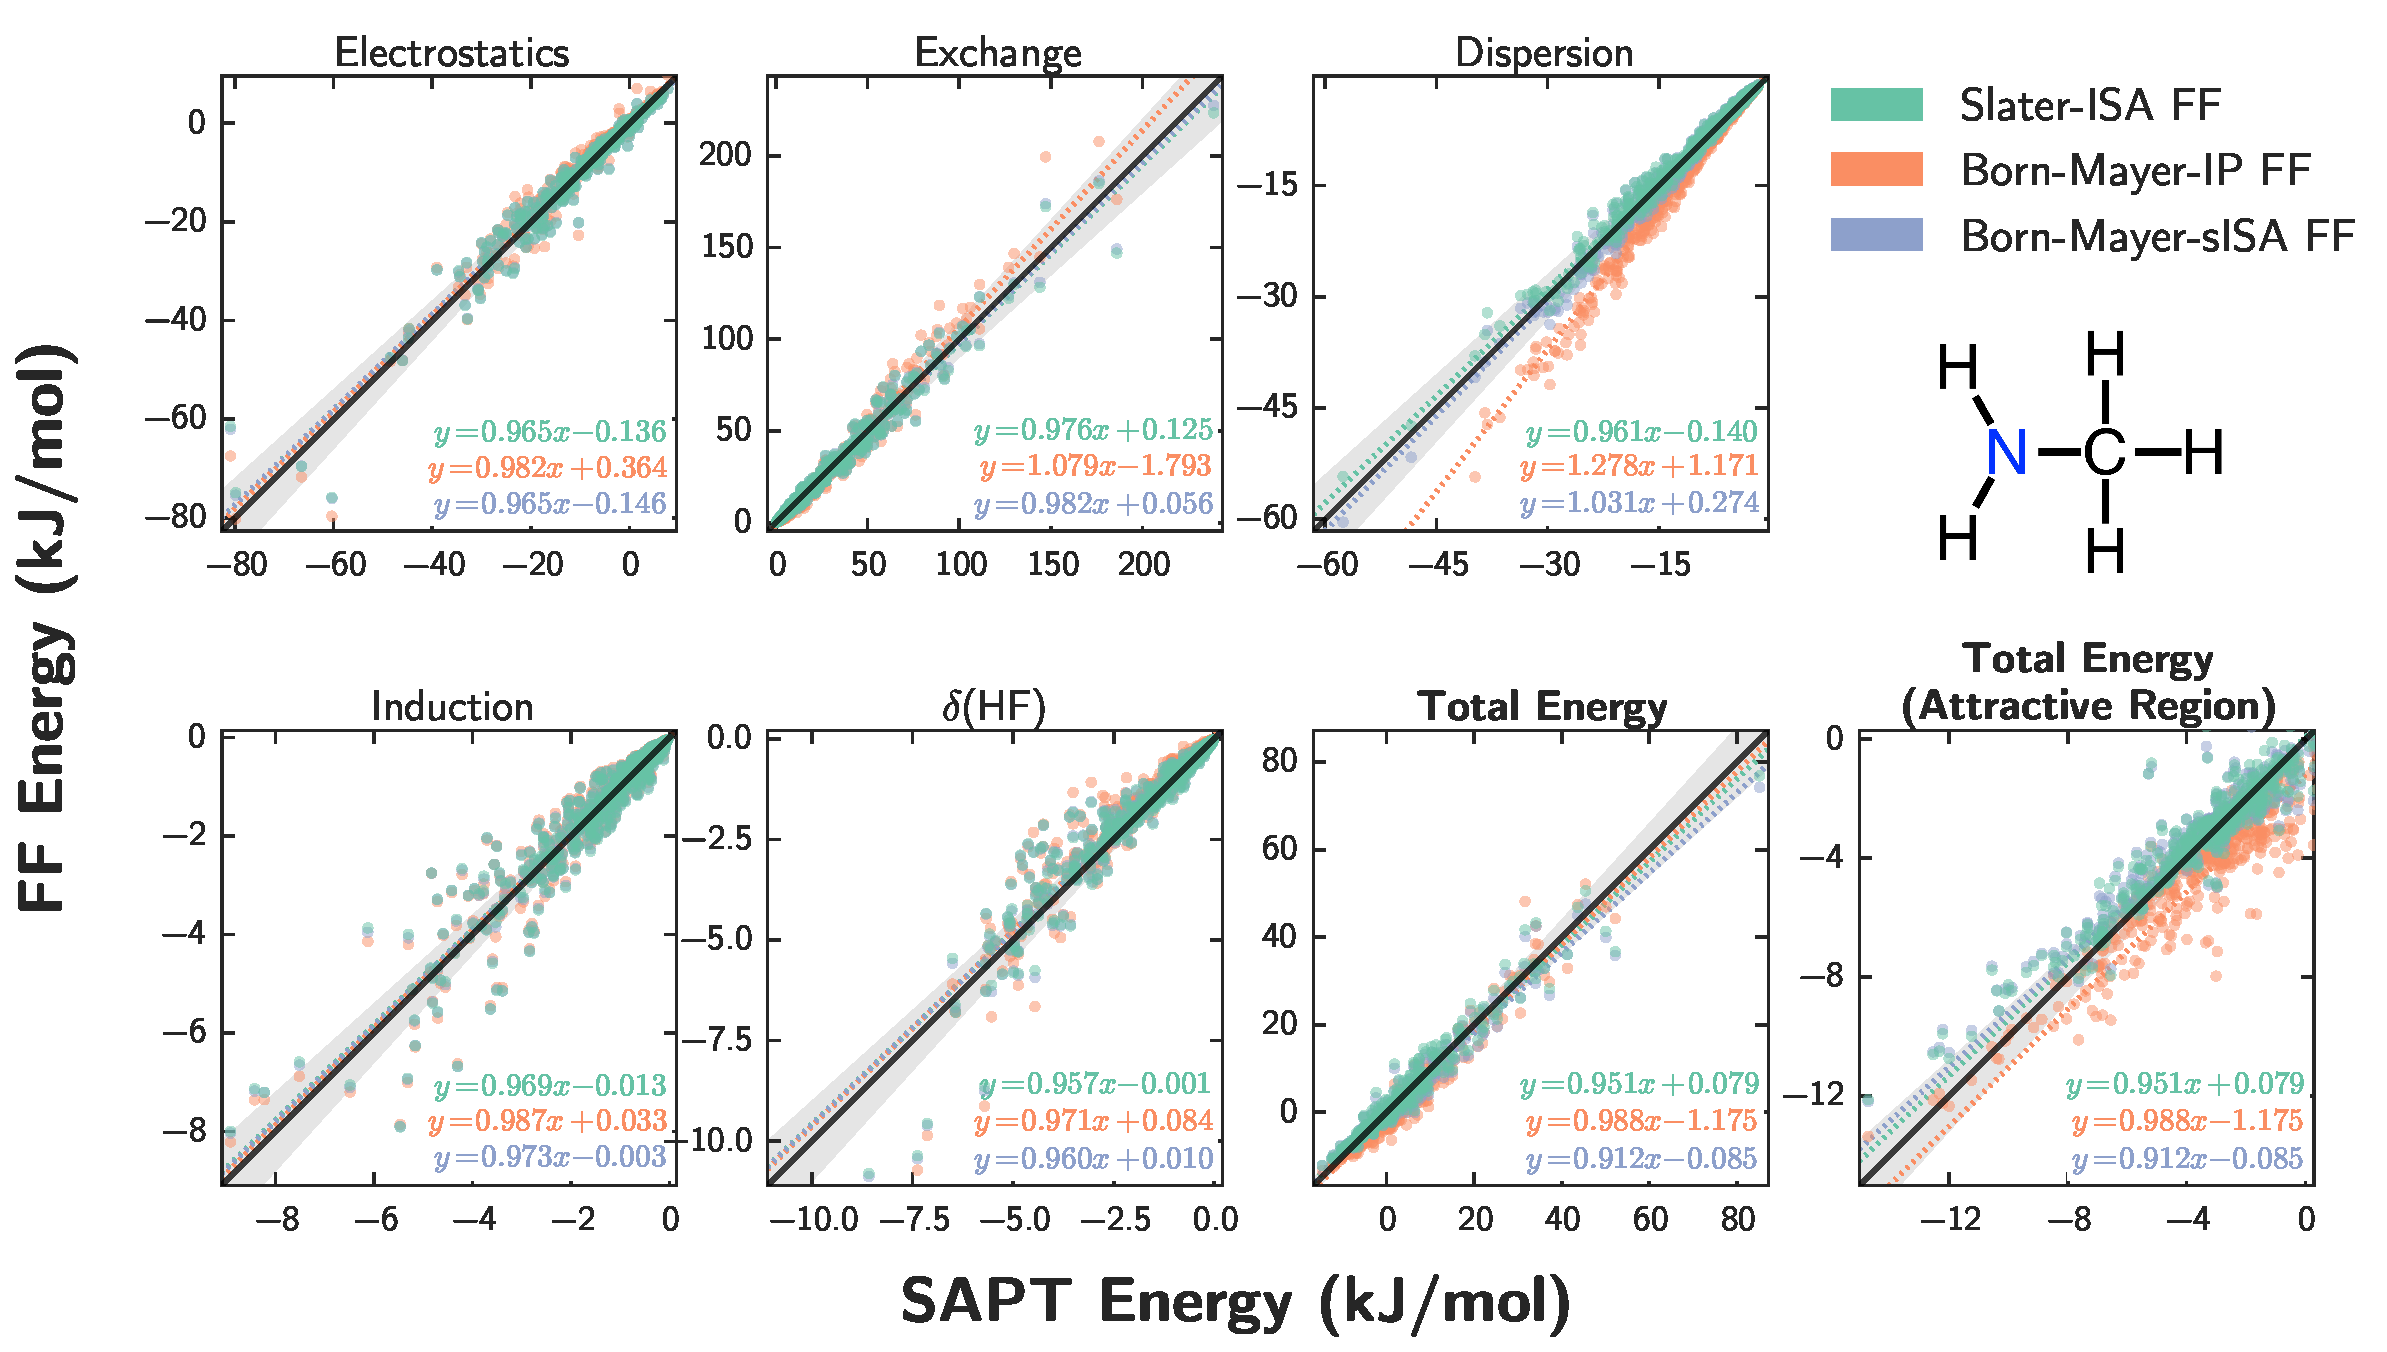
\includegraphics[width=0.9\textwidth]{isotropic/si/methyl_amine_methyl_amine_scatter.pdf}
    \end{subfigure}
    \end{figure}
    \begin{figure}
    \ContinuedFloat
    \begin{subfigure}{\textwidth}
        \caption{\nh Dimer}
        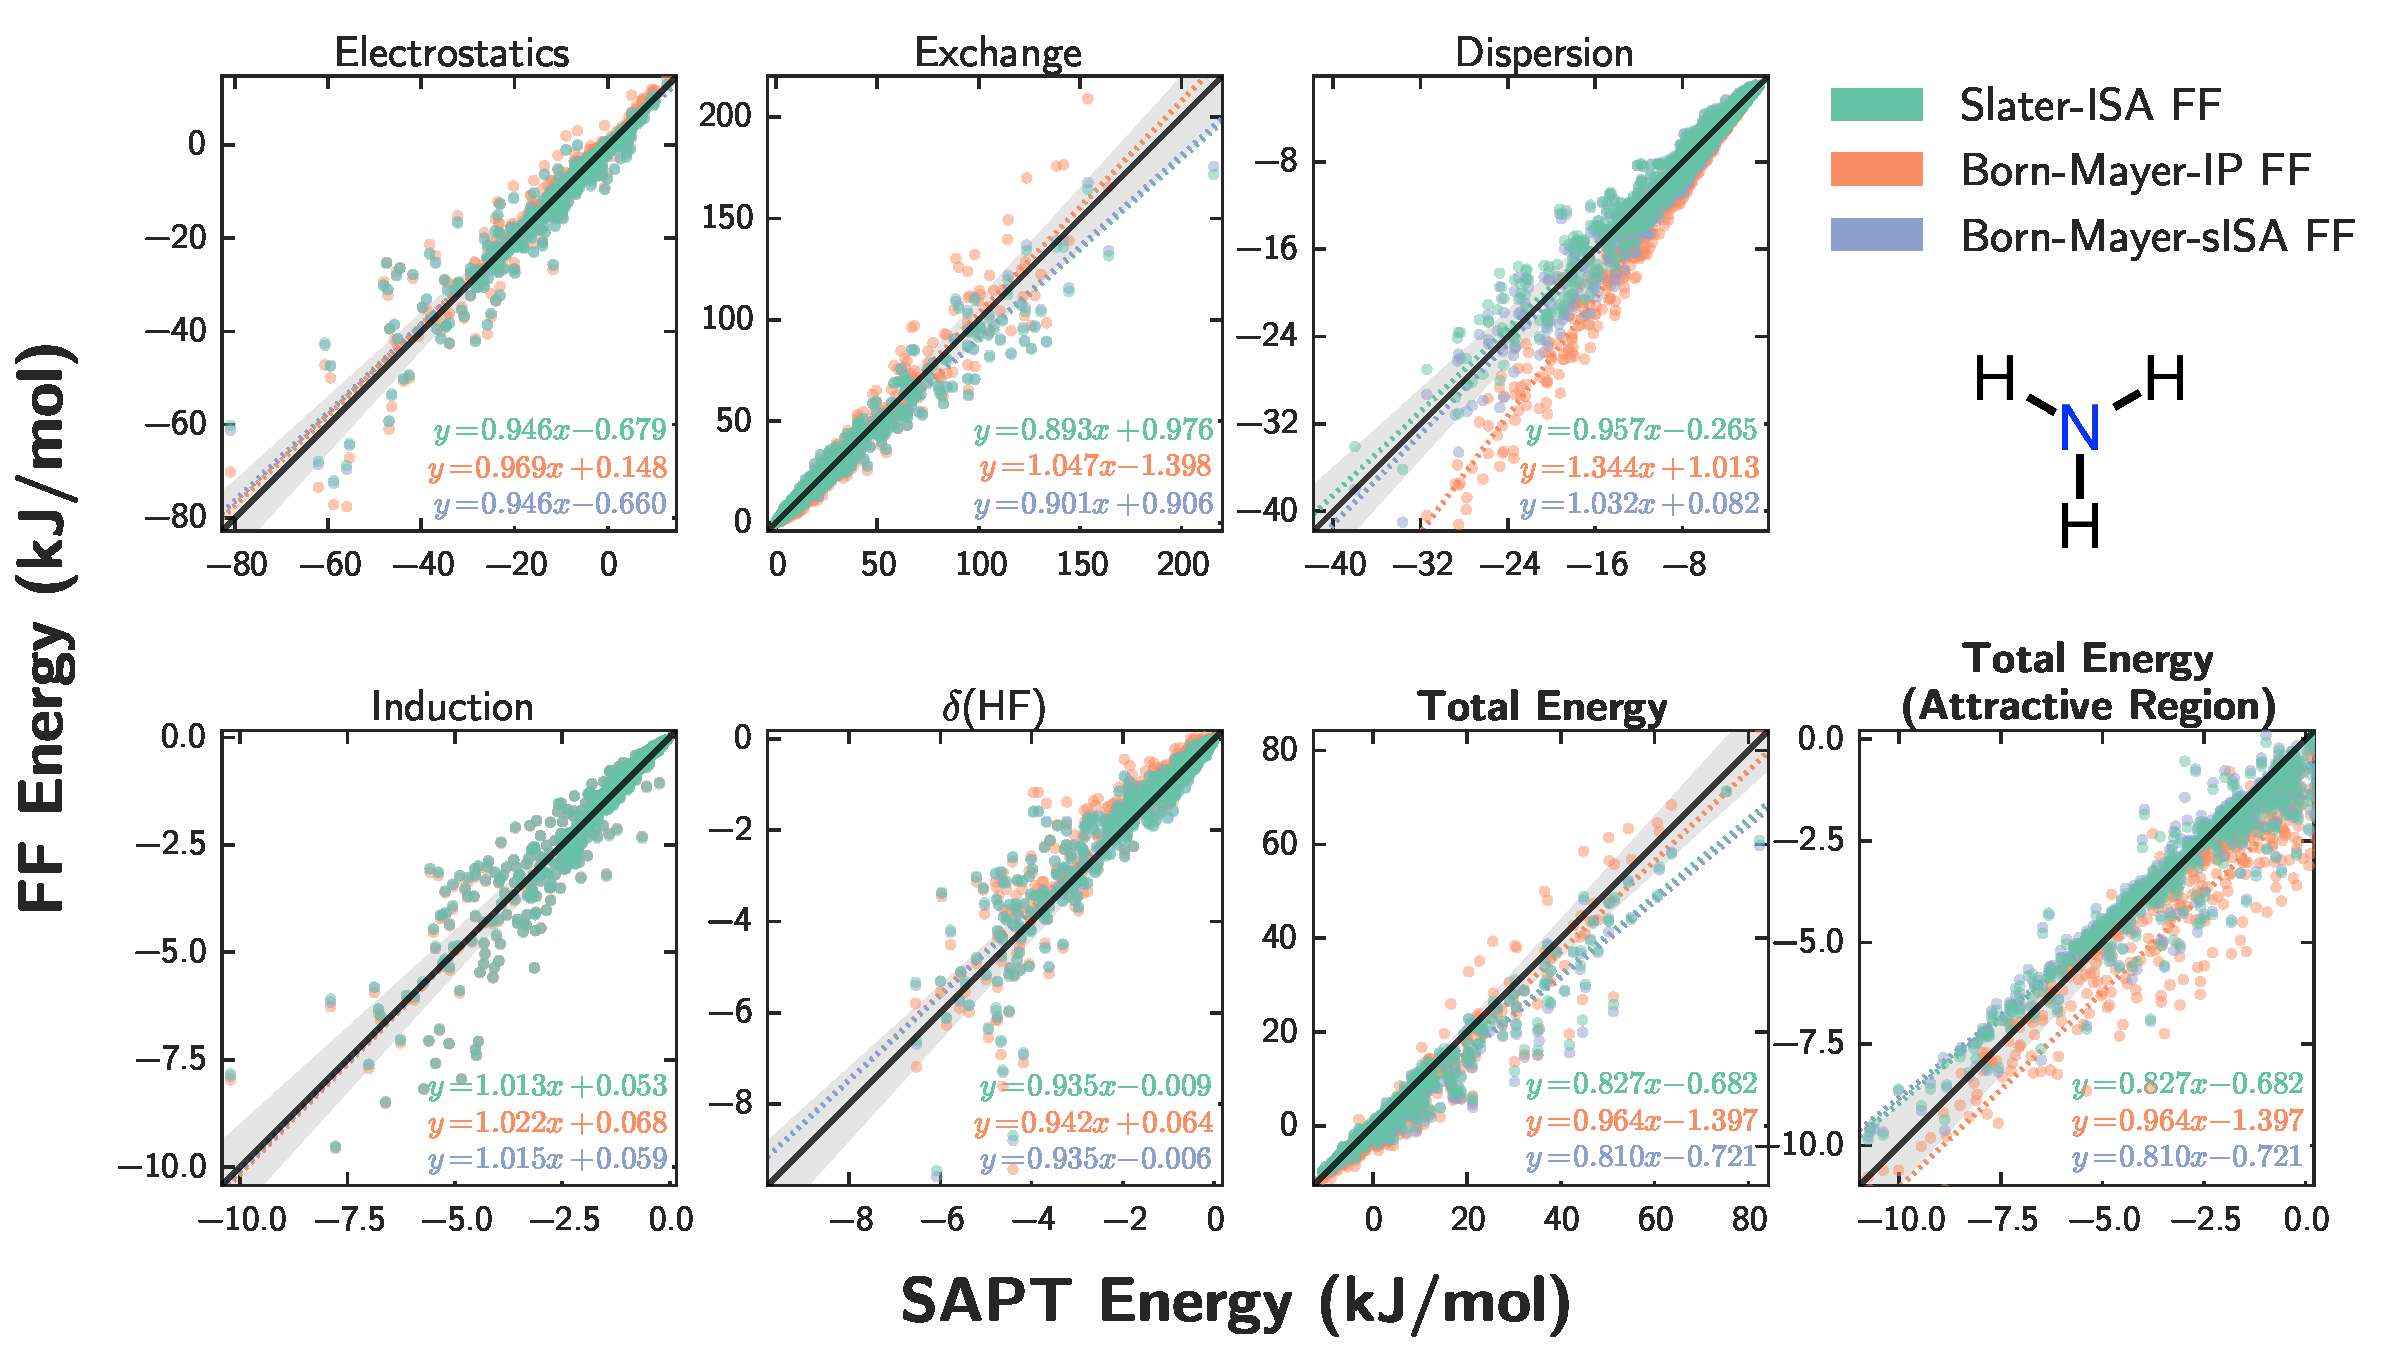
\includegraphics[width=0.9\textwidth]{isotropic/si/nh3_nh3_scatter.pdf}
    \end{subfigure}
    \caption{
    Force field fits for the homomoneric systems using the \isaffold (green), \saptff
(orange) and \bmsisaff (blue).
    Fits for each energy component are displayed along with two views of the total interaction energy.
    The $y=x$ line (black) indicates perfect agreement between reference energies
    and each force field, while shaded grey areas represent points within $\pm
    10\%$ agreement of the benchmark. To guide the eye, a line of best fit (dotted
    line) has been computed for each force field and for each energy component.
     }
    \label{fig:all-scatter}
    \end{figure}
    %%%%%%%% All Scatter %%%%%%%%%%






\end{section}
%% \clearpage
%% \begin{section}{Force Field Accuracy for \ljff}
%% 
%%     %%%%%%%%%%%% Ar-Ar PES %%%%%%%%%%%%%%%%%%
%%     \begin{figure}
%%     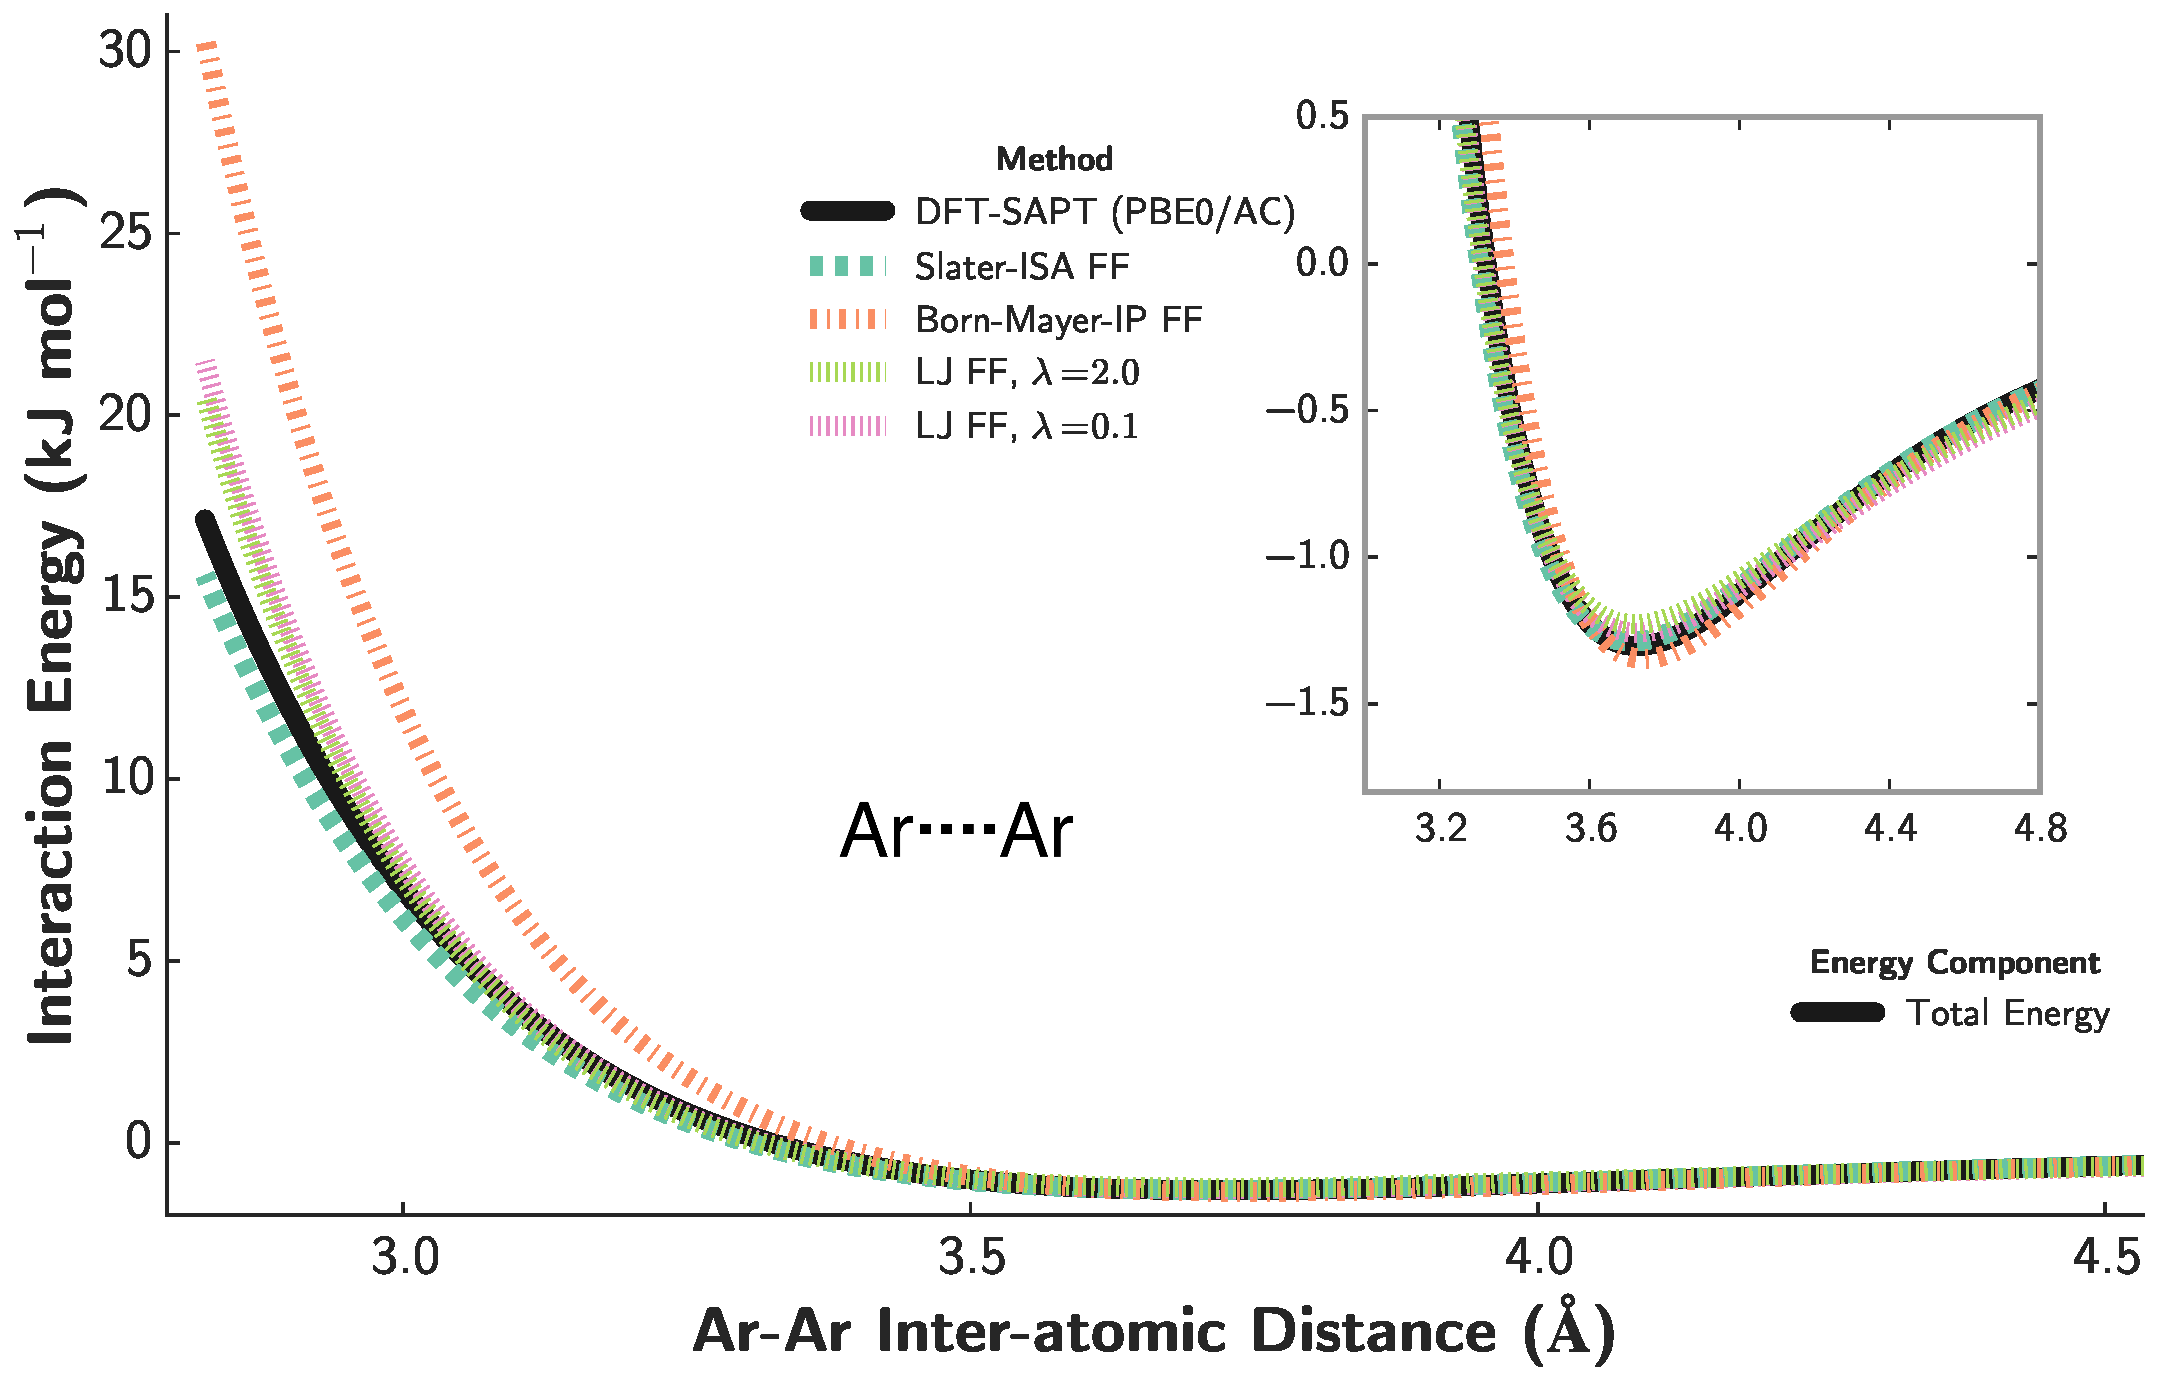
\includegraphics[width=0.9\textwidth]{isotropic/si/ar_ar_pes_wi_lj.pdf}
%%     \caption{
%%     Potential energy surface for the argon dimer. 
%%     Interaction energies for the \isaffold (dashed curves), \saptff (dash-dotted
%%     curves), and \ljff (dotted curves) are shown alongside benchmark \saptpbeo energies (solid curves). 
%%     Note that, for the \ljff force fields, 
%%     the magnitude of the attractive tail region is overestimated by the
%%     effective $C_{ij,6}$ dispersion parameter.
%%     }
%%     \label{fig:ar-pes}
%%     \end{figure}
%%     %%%%%%%%%%%% Ar-Ar PES %%%%%%%%%%%%%%%%%%
%% 
%% 
%%     %%%%%%%% Ethane-Ethane Scatter %%%%%%%%%%
%%     \begin{figure}
%%     %\includegraphics[width=0.9\textwidth]{isotropic/si/ammonia_ff_quality.png}
%%     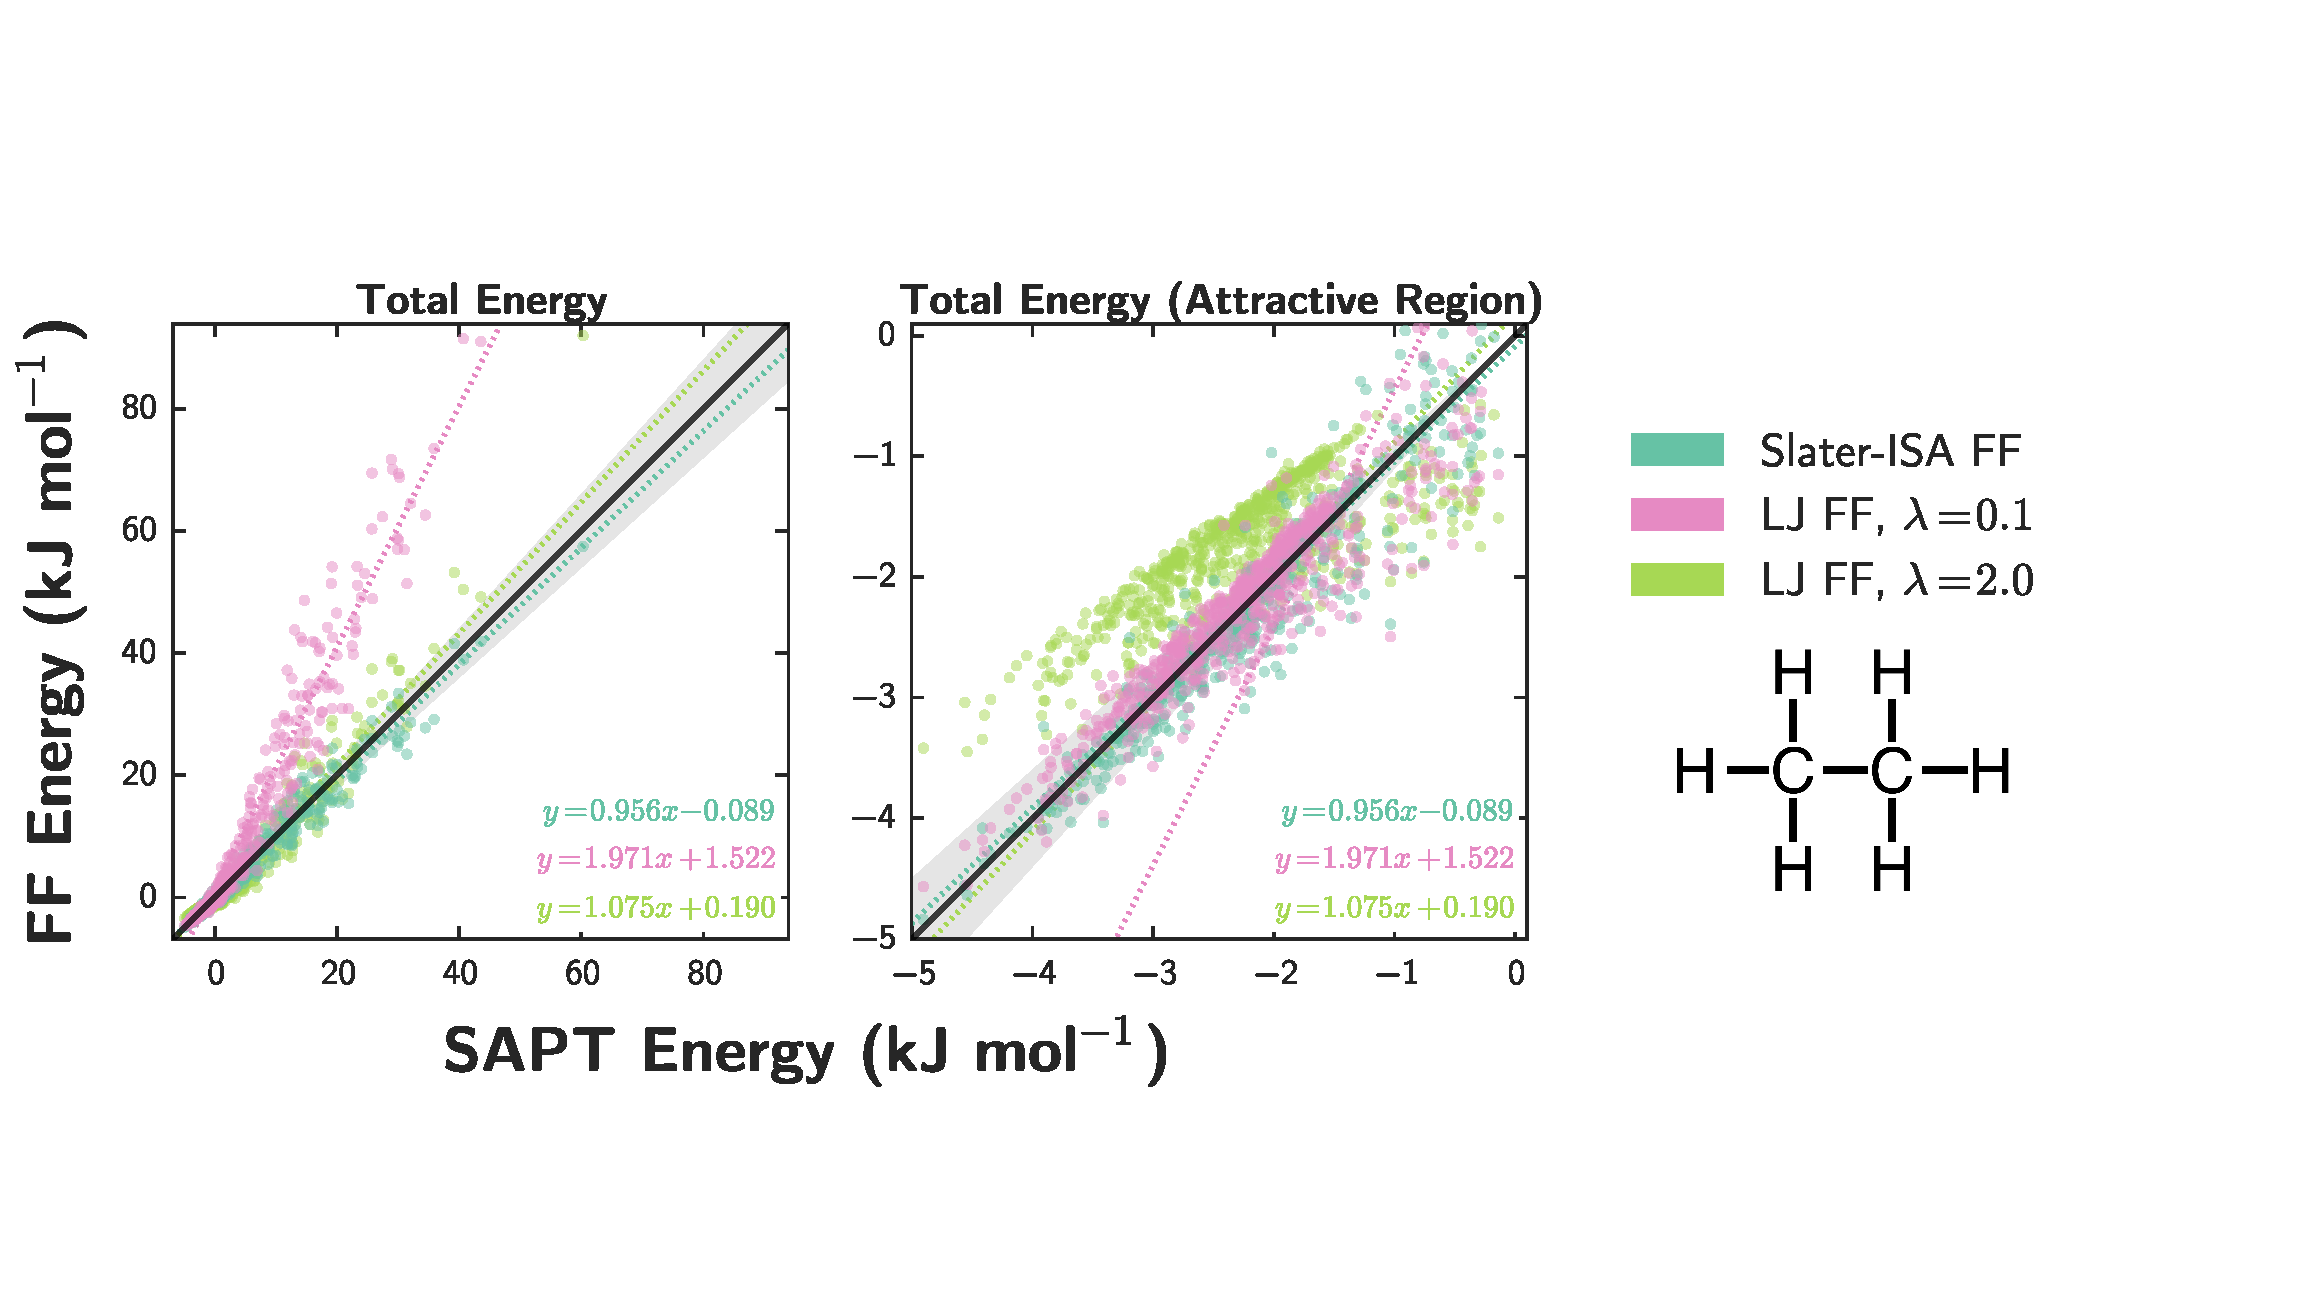
\includegraphics[width=0.9\textwidth]{isotropic/si/ethane_ethane_lj_scatter.pdf}
%%     \caption[foo]{
%%     Fits for two views of the total interaction energy for 
%%     the ethane dimer using the Slater-ISA (teal),
%%     LJ $\lambda = 0.1$ (pink) and LJ $\lambda = 2.0$ (lime green) FFs.
%%     The diagonal line (black) indicates perfect agreement between reference energies
%%     and each force field, while shaded grey areas represent points within $\pm
%%     10\%$ agreement of the benchmark. To guide the eye, a line of best fit (dotted
%%     line) has been computed for each force field.
%%      }
%%     \label{fig:ethane-scatter}
%%     \end{figure}
%%     %%%%%%%% Ethane-Ethane Scatter %%%%%%%%%%
%% 
%%     %%%%%%%%%%% Ethane-Ethane PES %%%%%%%%%%%
%%     \begin{figure}
%%     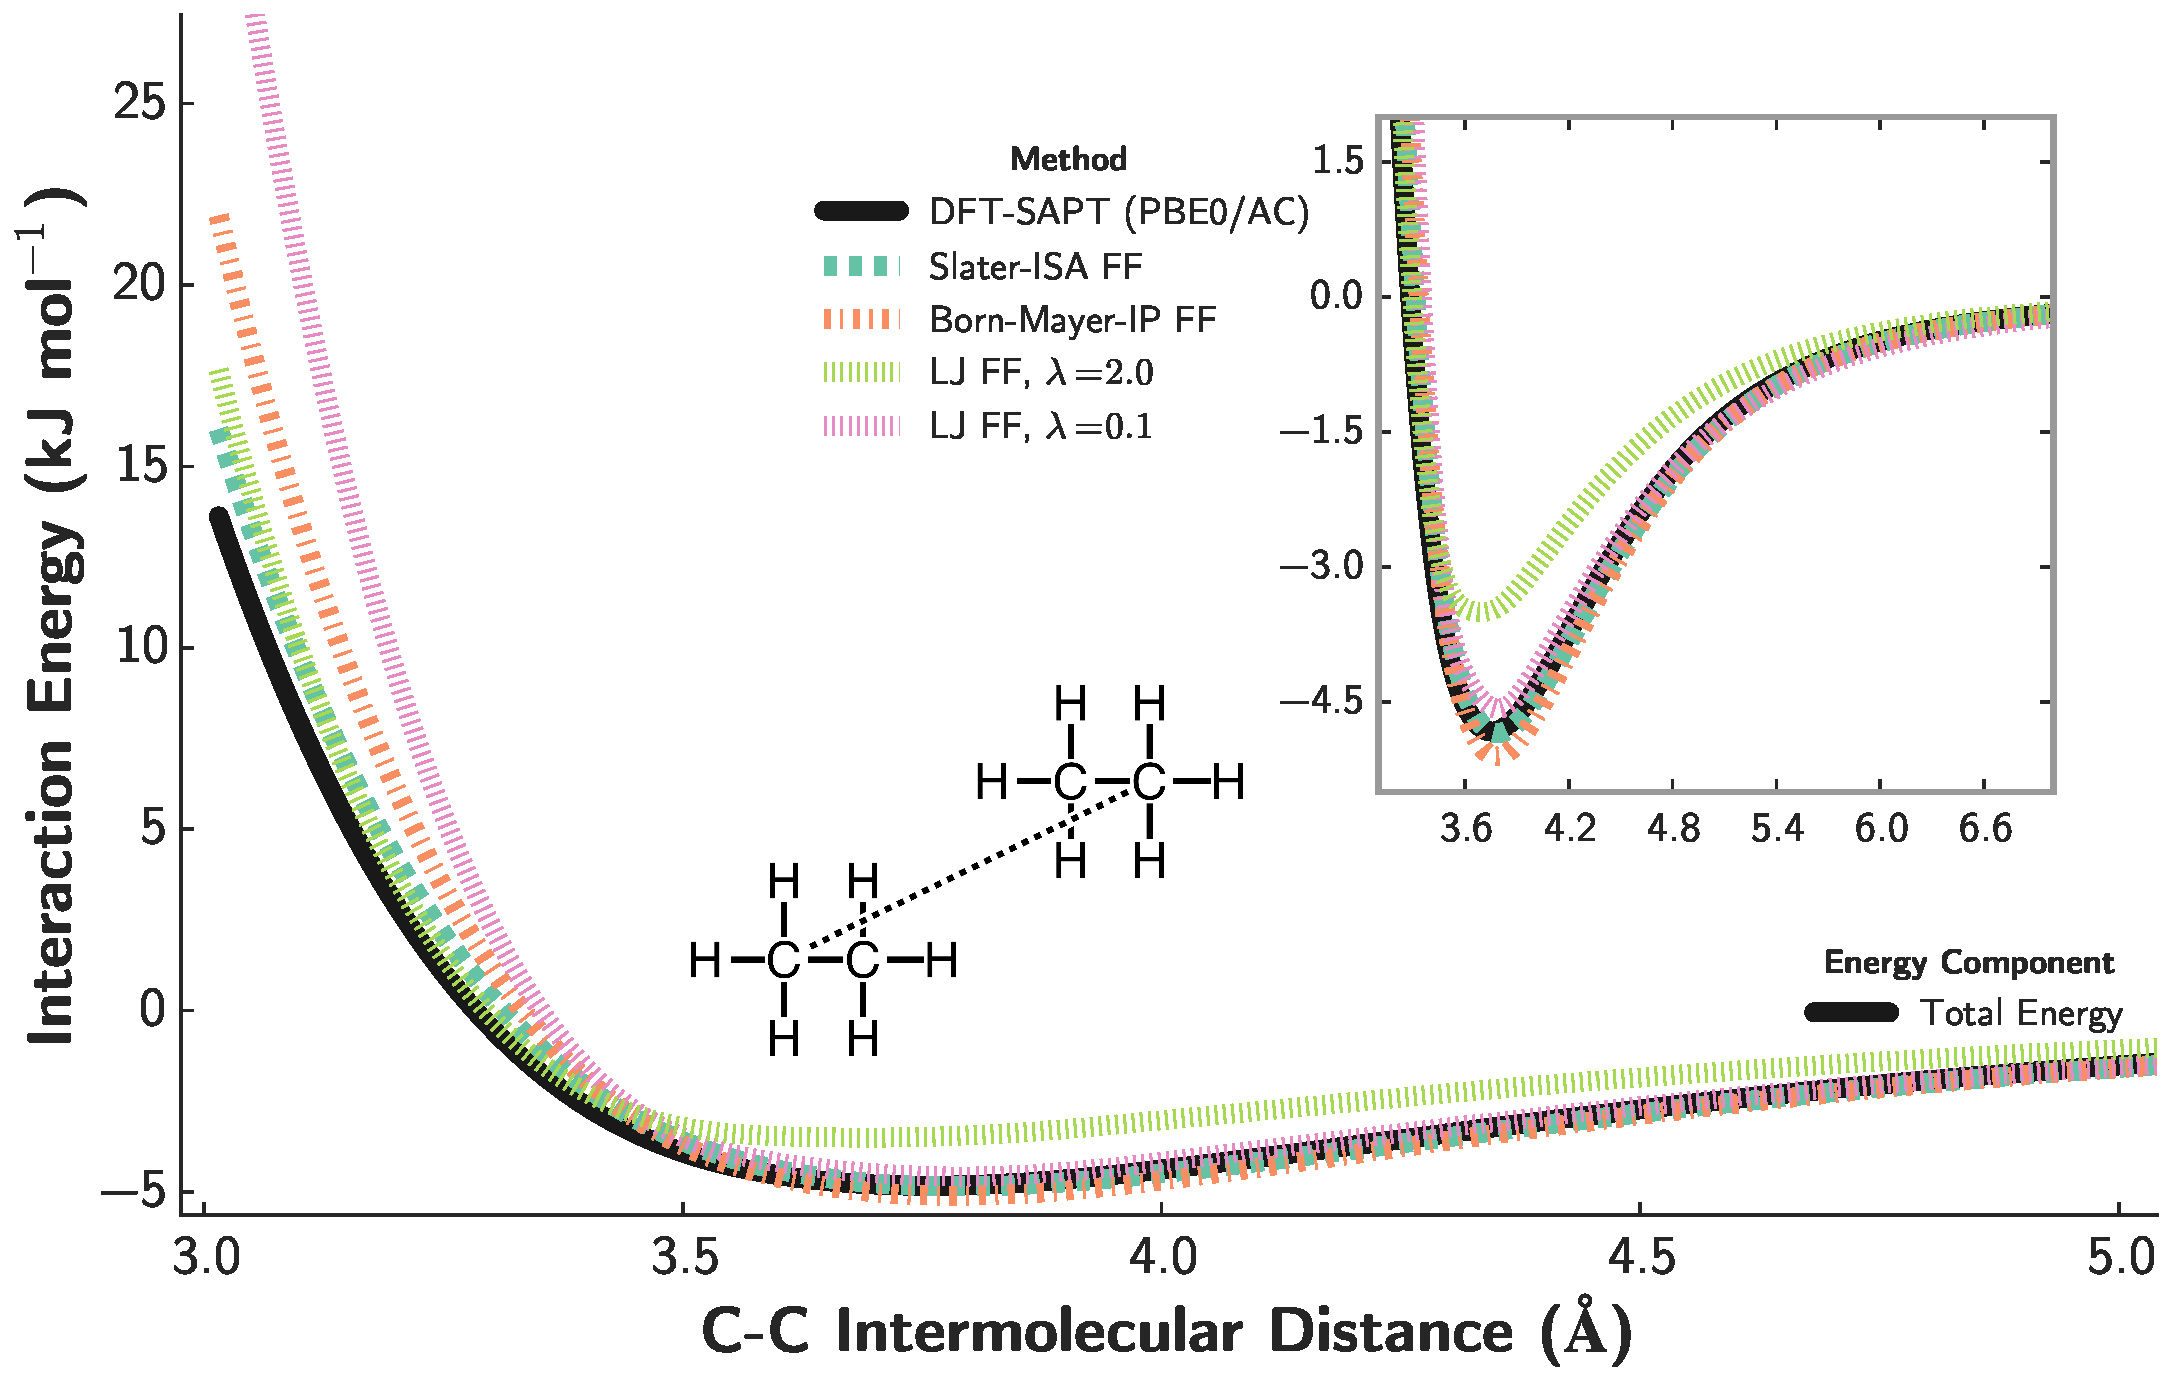
\includegraphics[width=0.9\textwidth]{isotropic/si/ethane_ethane_pes_wi_lj.pdf}
%%     \caption{
%%     A representative potential energy scan near a local minimum for the ethane dimer. 
%%     Interaction energies for the \isaffold (dashed curves), \saptff (dash-dotted
%%     curves), and \ljff (dotted curves)  are shown alongside benchmark \saptpbeo energies (solid curves). The
%%     energy decomposition for DFT-SAPT and for each force field is shown for reference.
%%      The ethane dimer configuration in this scan corresponds to the most
%%     energetically attractive dimer included in the training set; other
%%     points along this scan are not included in the training set.
%%     }
%%     \label{fig:ethane-pes}
%%     \end{figure}
%%     %%%%%%%%%%% Ethane-Ethane PES %%%%%%%%%%%
%% 
%%     %%%%%%%% Acetone-Acetone Scatter %%%%%%%%%%
%%     \begin{figure}
%%     %\includegraphics[width=0.9\textwidth]{isotropic/si/ammonia_ff_quality.png}
%%     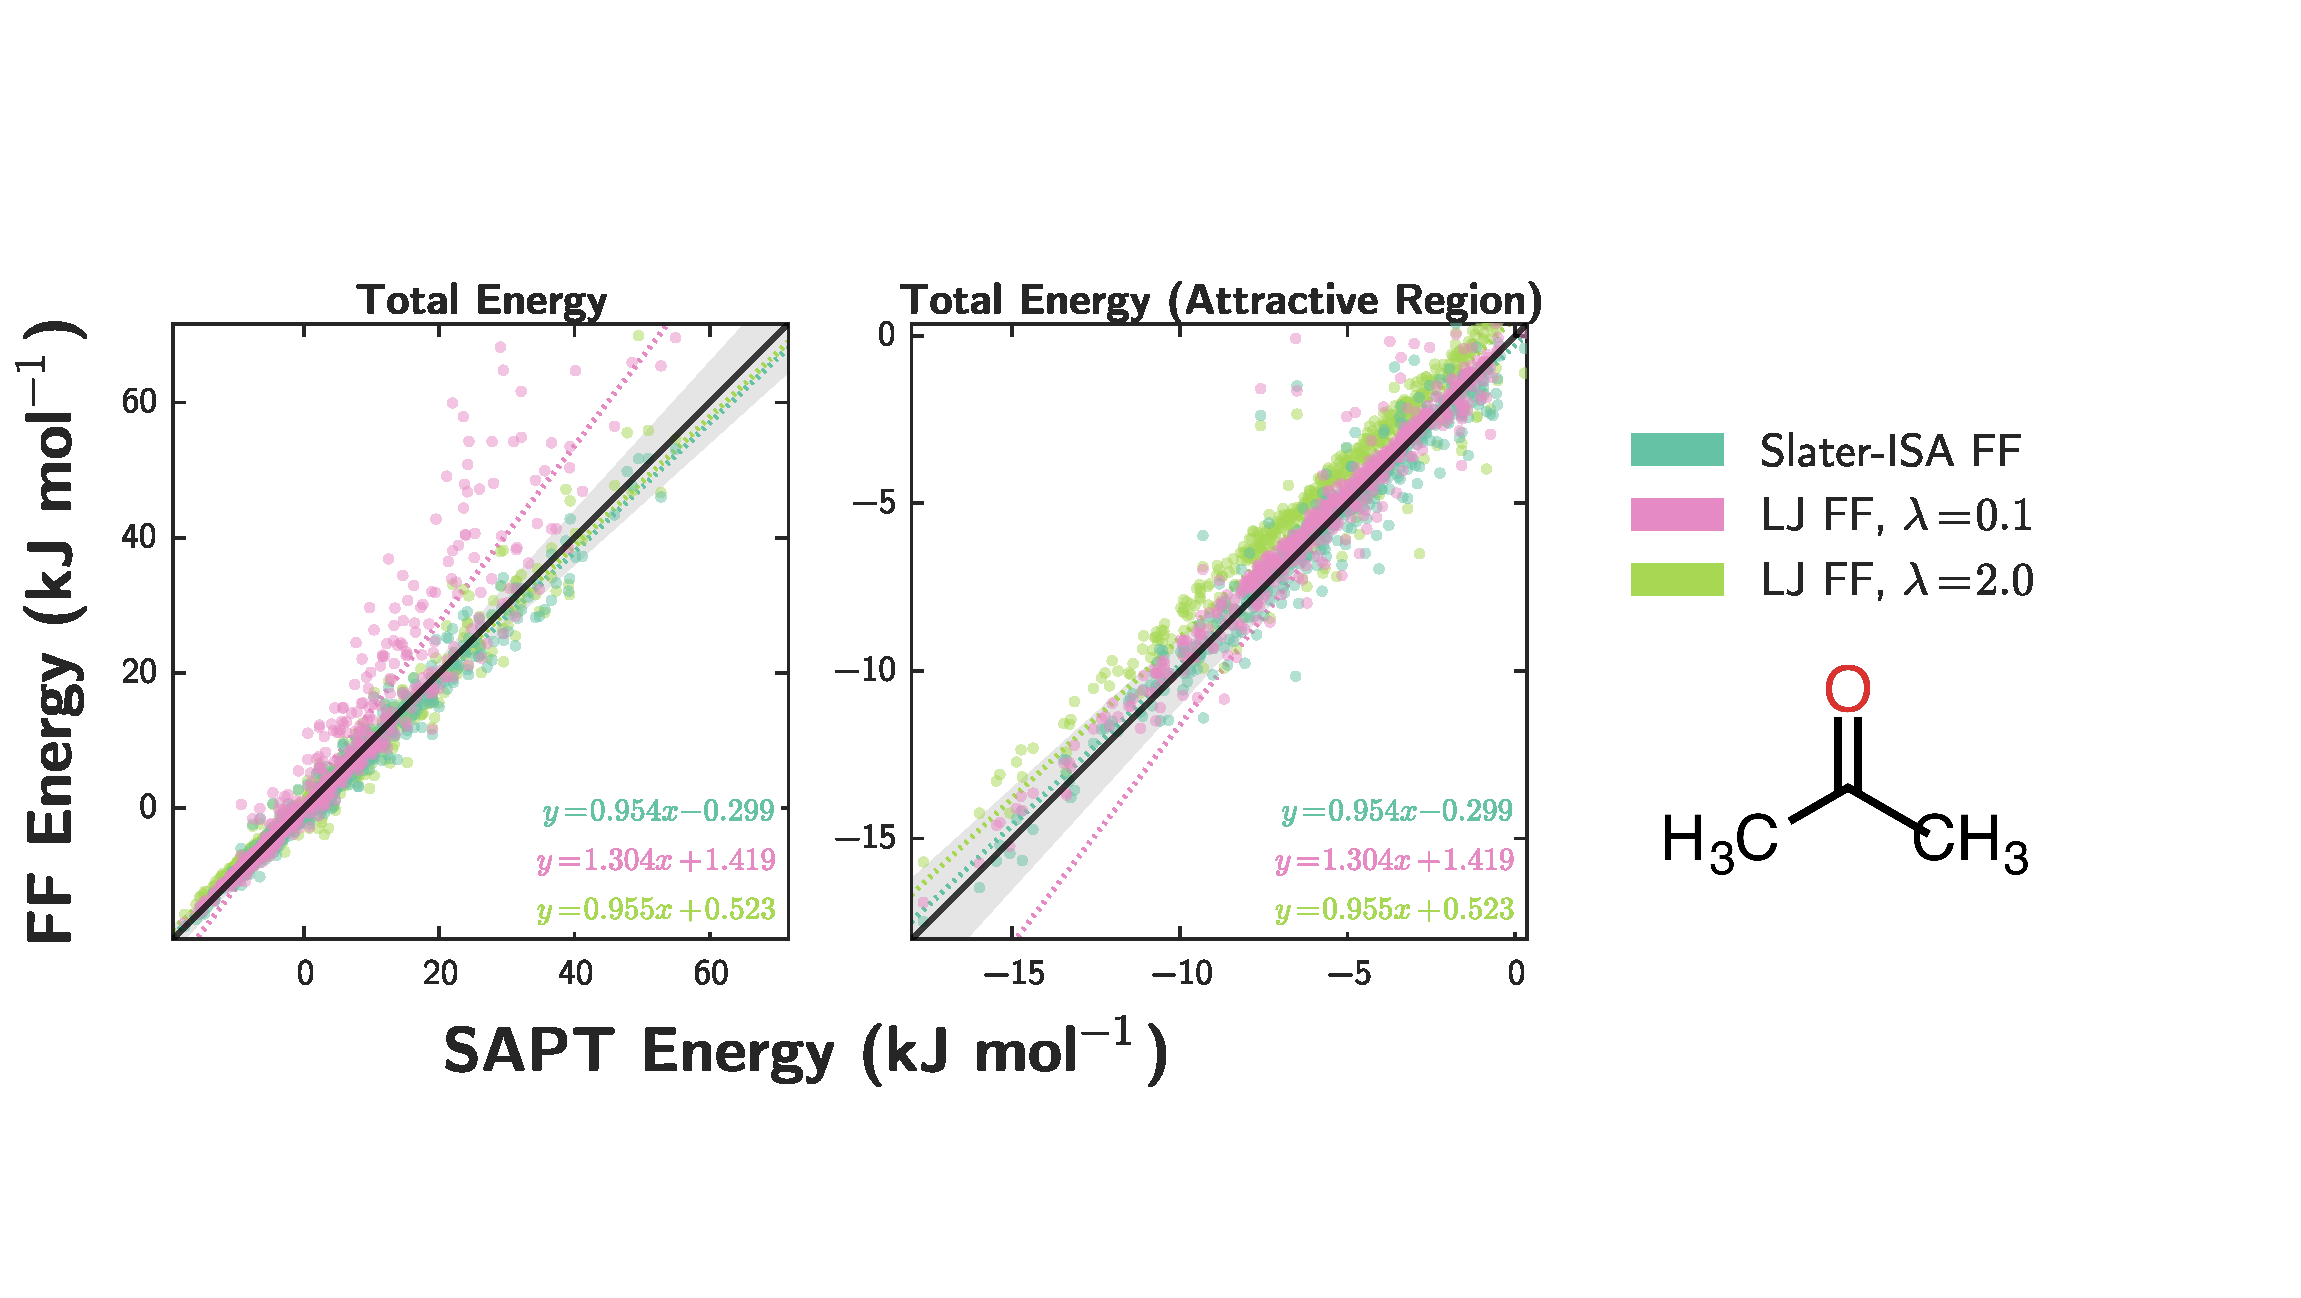
\includegraphics[width=0.9\textwidth]{isotropic/si/acetone_acetone_lj_scatter.pdf}
%%     \caption{
%%     Force field fits for the acetone dimer using the Slater-ISA (teal), LJ
%% $\lambda = 0.1$ (pink) and LJ $\lambda = 2.0$ (lime green) FFs.
%%     Fits for two views of the total interaction energy are displayed.
%%     The diagonal line (black) indicates perfect agreement between reference energies
%%     and each force field, while shaded grey areas represent points within $\pm
%%     10\%$ agreement of the benchmark. To guide the eye, a line of best fit (dotted
%%     line) has been computed for each force field.
%%      }
%%     \label{fig:acetone-scatter}
%%     \end{figure}
%%     %%%%%%%% Acetone-Acetone Scatter %%%%%%%%%%
%% 
%%     %%%%%%%%%%% Acetone-Acetone PES %%%%%%%%%%%
%%     \begin{figure}
%%     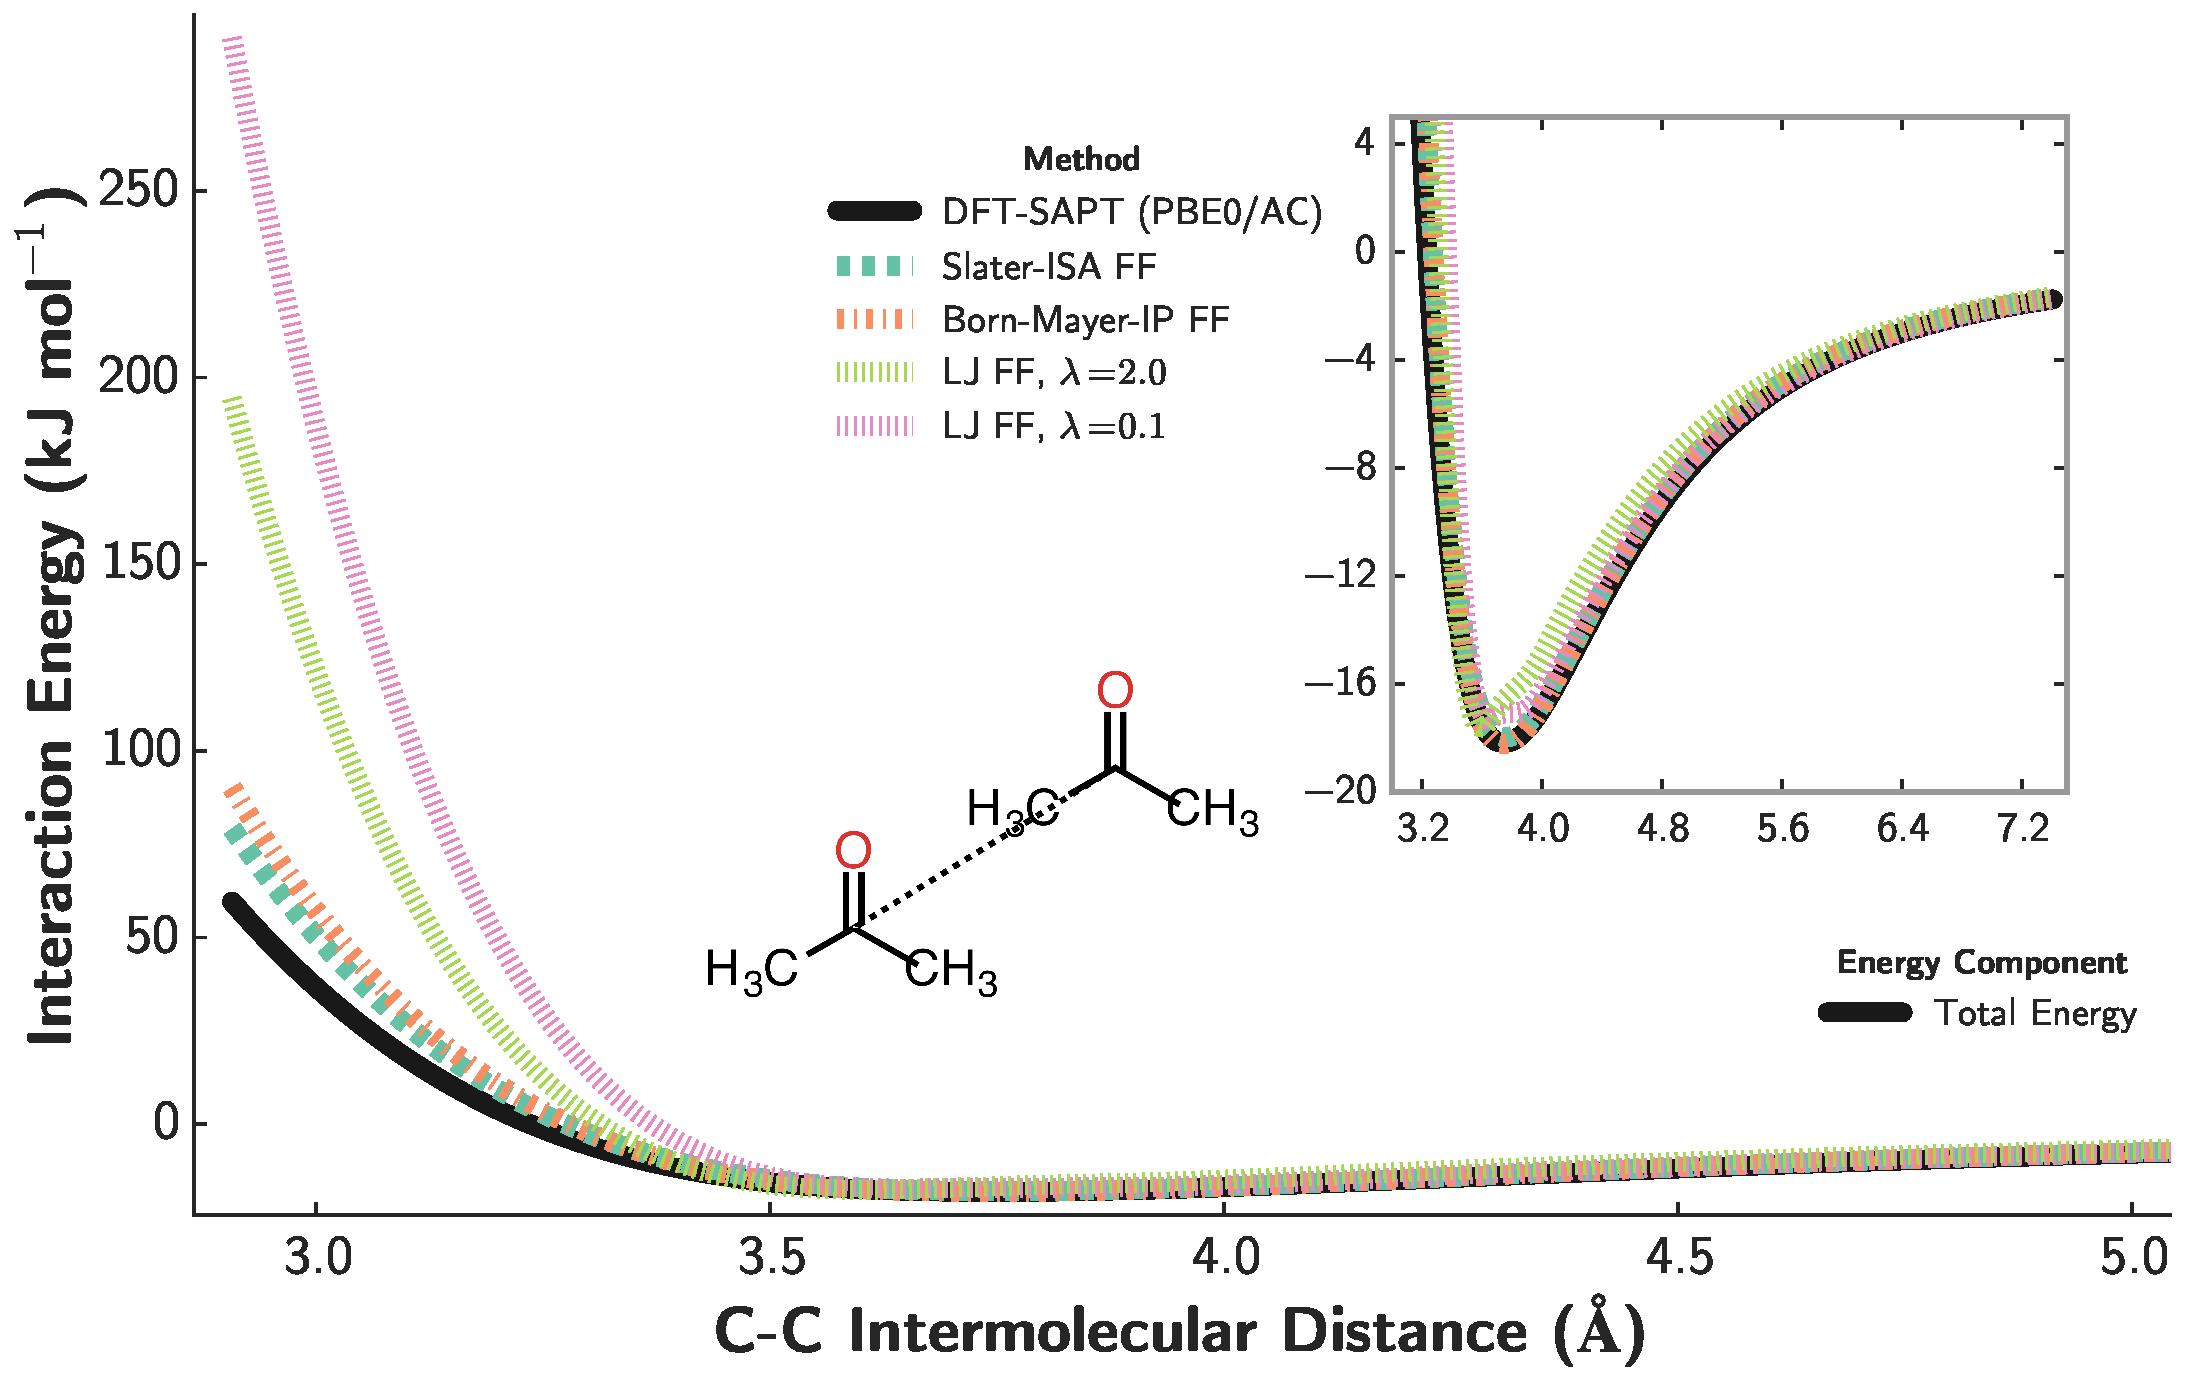
\includegraphics[width=0.9\textwidth]{isotropic/si/acetone_acetone_pes_wi_lj.pdf}
%%     \caption{
%%     A representative potential energy scan near a local minimum for the acetone dimer. 
%%     Interaction energies for the \isaffold (dashed curves), \saptff (dash-dotted
%%     curves), and \ljff (dotted curves) are shown alongside benchmark \saptpbeo energies (solid curves). The
%%     energy decomposition for DFT-SAPT and for each force field is shown for reference.
%%       The intermolecular distance is taken to be the
%%       internuclear distance between the two carbonyl carbons on each acetone
%%       monomer.  
%%      The acetone dimer configuration in this scan corresponds to the most
%%     energetically attractive dimer included in the training set; other
%%     points along this scan are not included in the training set.
%%     }
%%     \label{fig:acetone-pes}
%%     \end{figure}
%%     %%%%%%%%%%% Acetone-Acetone PES %%%%%%%%%%%
%% 
%% 
%% \end{section}
%% \clearpage
%% \begin{section}{Parameter Robustness for Argon}
%% 
%% Argon parameters were tested for robustness by changing the weighting function
%% as described in the main text. As with ethane, optimized \isaffold \A parameters are
%% much less sensitive to the choice of weighting function compared to
%% the \saptff. As a result, the \isaffold shows decreased uncertainty when computing
%% the 2\super{nd} virial coefficient. Virial coefficients for the \saptff, on the
%% other hand, depend more strongly on the choice of weighting function. The
%% fortuitous agreement with experiment for the \saptff with $\lambda = 0.5$ may
%% point to inaccuracies in the DFT-SAPT potential itself, but is not indicative of
%% enhanced force field fitting quality. (Indeed,
%% \ref{fig:ar-weighting} shows that this weighting function leads to the worst
%% agreement with DFT-SAPT compared to other $\lambda$ values). Overall, the
%% argon fits demonstrate increased parameter robustness for the \isaffold.
%% 
%% 
%%     %%%%%%%% Weighting Function Tests %%%%%%%
%%     \begin{figure}
%%     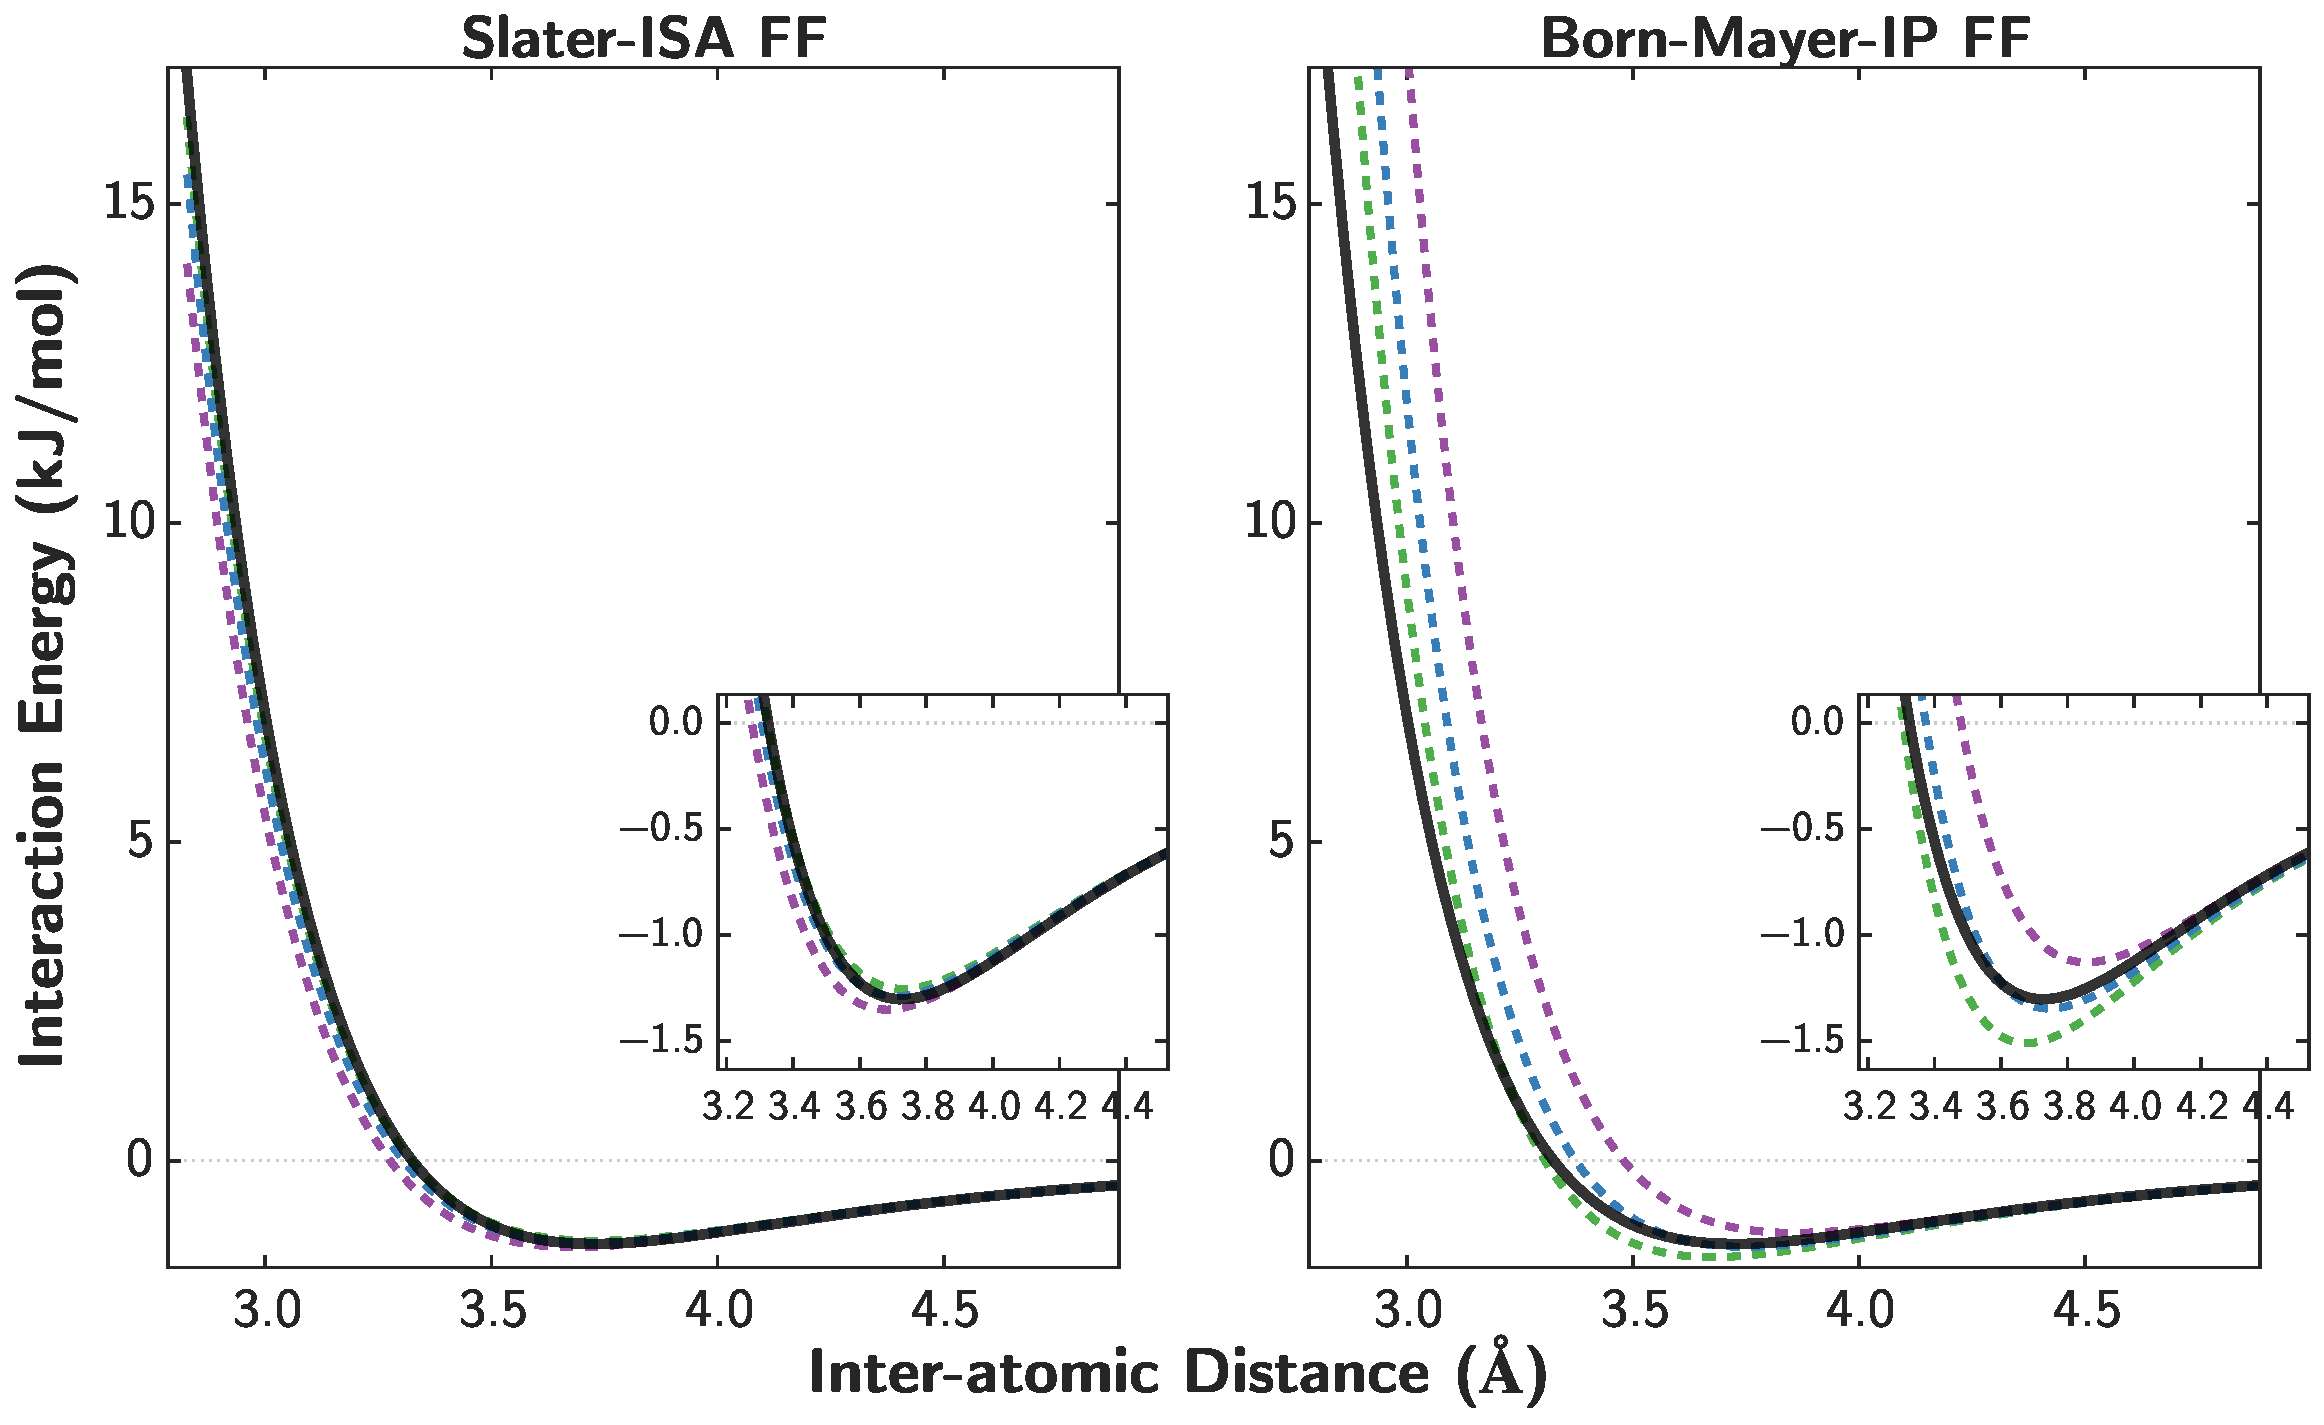
\includegraphics[width=0.8\textwidth]{isotropic/si/compare_ar_ar_scan.pdf}
%%     \vspace{10 mm}
%%     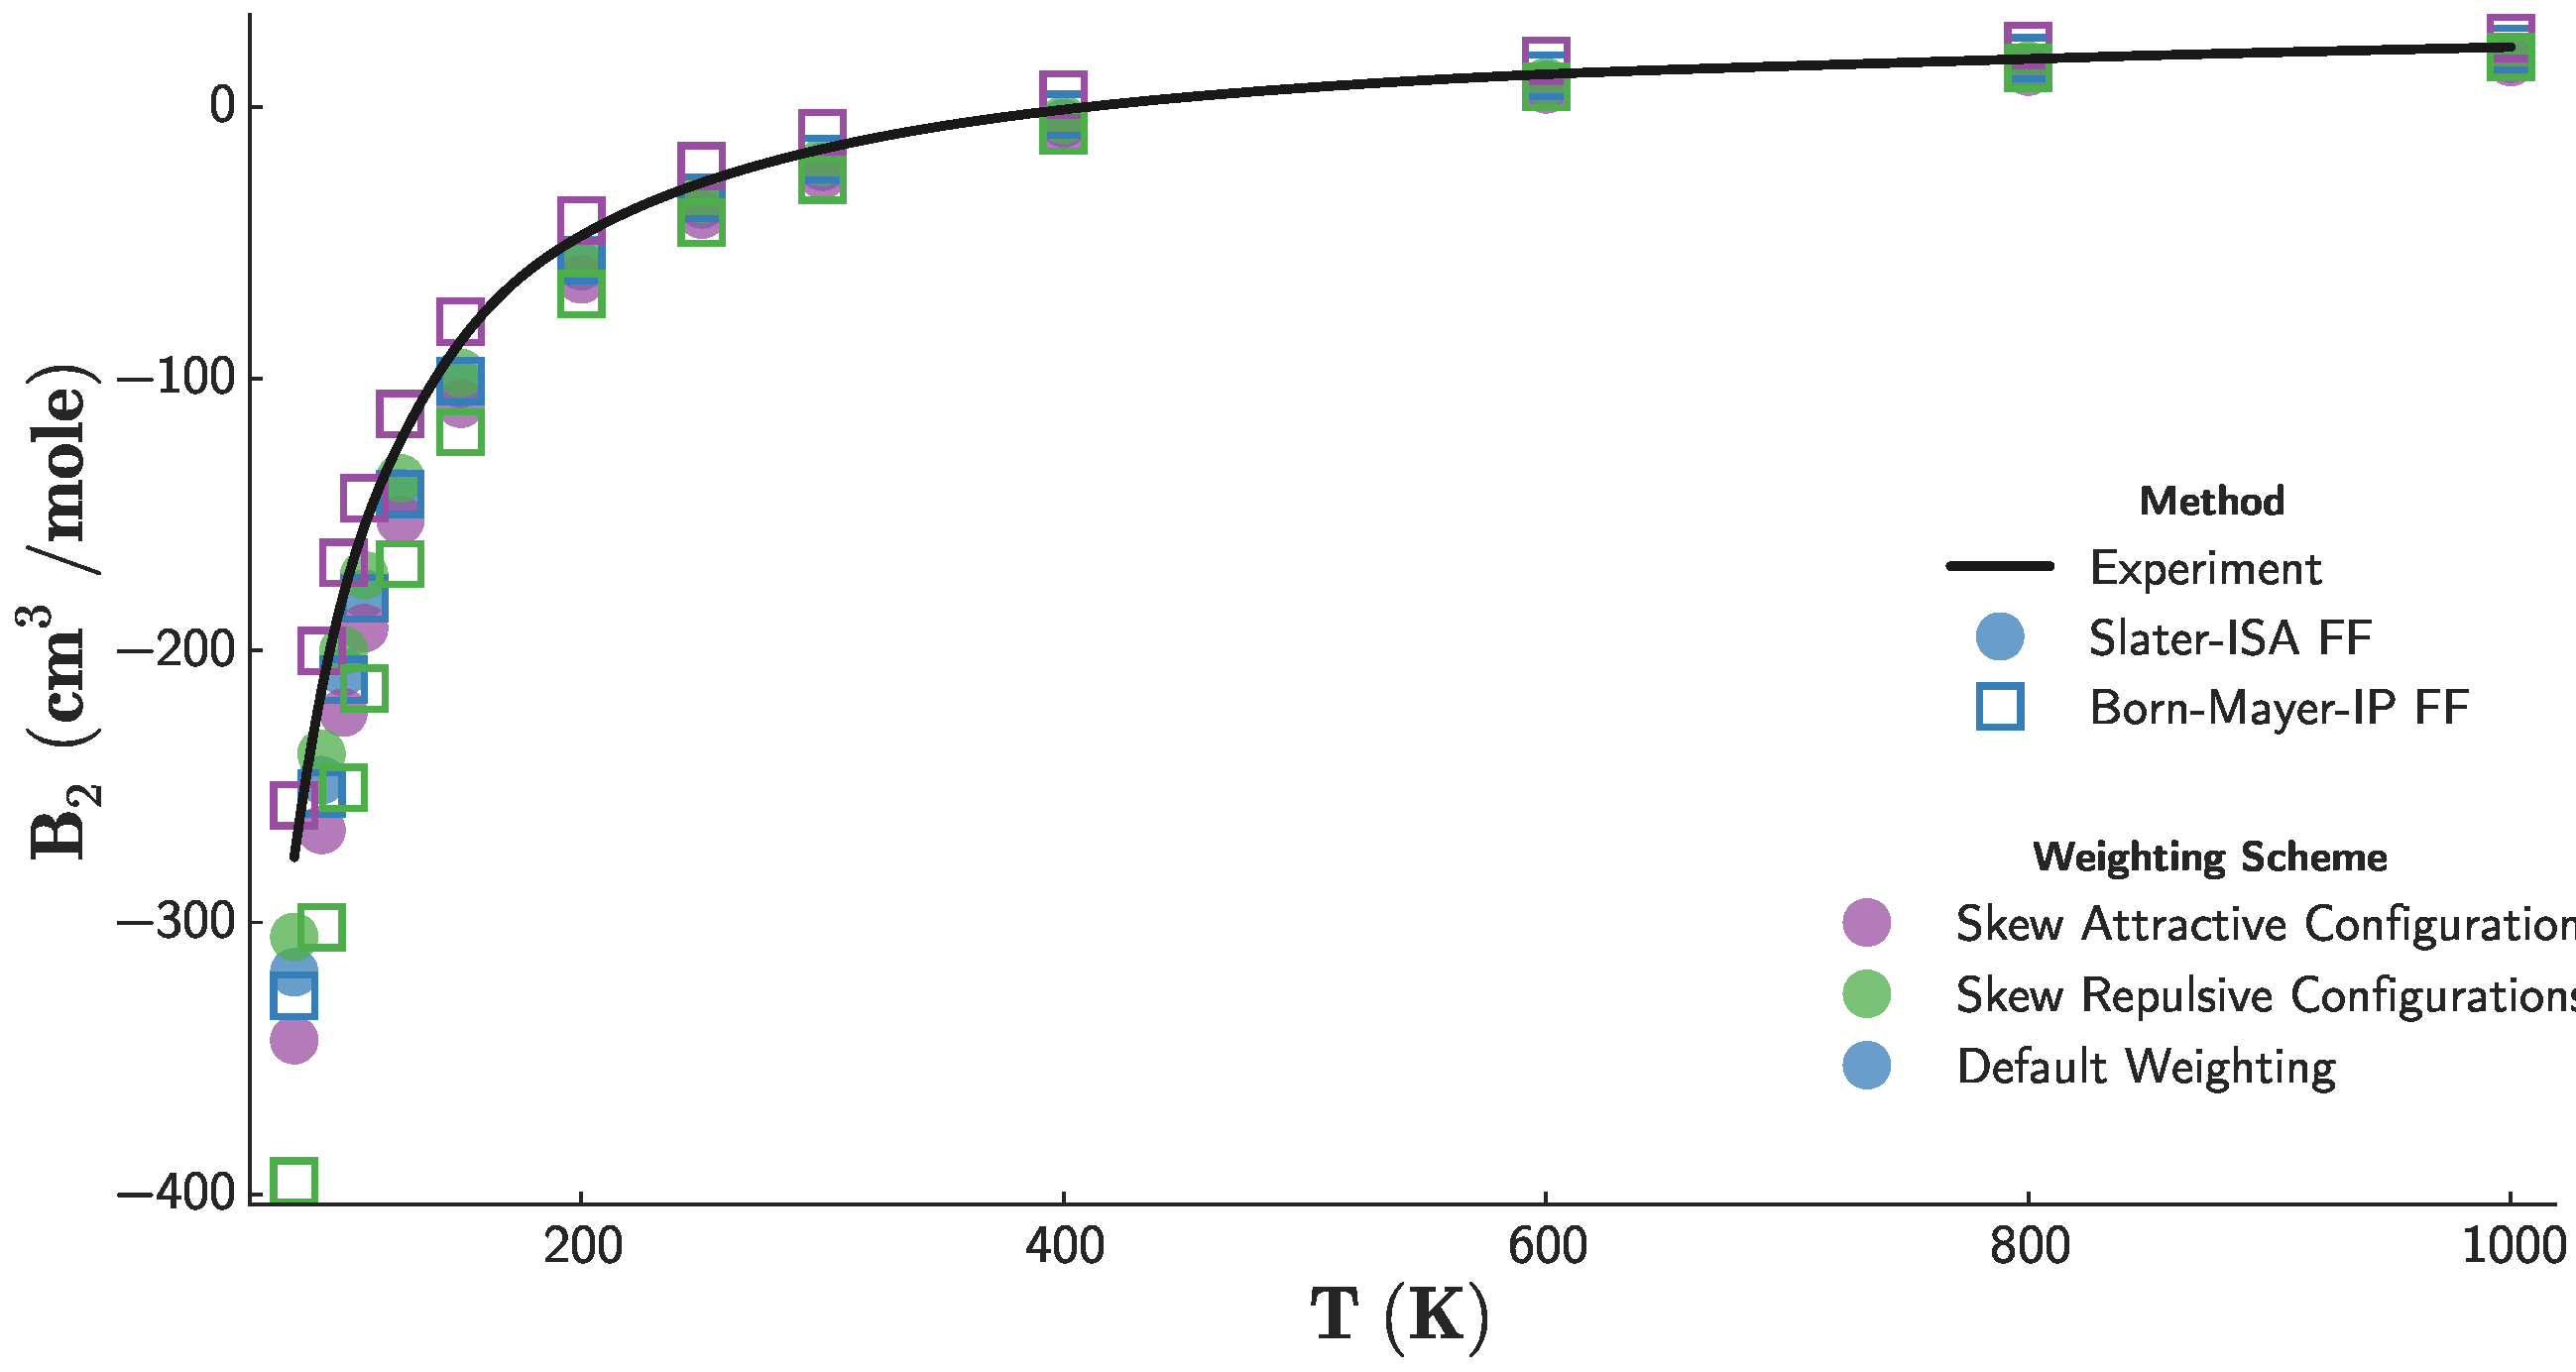
\includegraphics[width=0.8\textwidth]{isotropic/si/weighted_ar_2nd_virial.pdf}
%%     \caption[foo]{
%%         Comparison of the \isaffold and the \saptff in terms of sensitivity to the
%%         weighting function employed in parameter optimization for the Ar 
%%         dimer. Three weighting functions, $\lambda = 0.5$ (purple), $\lambda = 2.0$
%%         (blue), and $\lambda = 5.0$ (green) are shown, with higher $\lambda$ values
%%         indicating more weighting of repulsive configurations.
%%               
%%         (top) Total interaction energies for the \isaffold (left) and the \saptff (right)
%%         indicating the accuracy of each force field with respect to \saptpbeo benchmark
%%         energies. DFT-SAPT energies are shown as black solid lines, force field fits with
%%         dotted lines. Colors for the different weighting functions is as above.
%%               
%%         (bottom) Computed 2$^\text{nd}$ virial coefficients for argon. Data for
%%         the \isaffold and \saptff are depicted using open circles and shaded squares,
%%         respectively; coloration for the different weighting functions is as above.
%%         Experimental data from \citeauthor{Dymond1980} (black line) is also shown.
%%       %ASK: Do we actually cite Dymond and Smith for this, since it's a compiled
%%       %work, or do I need to try and dig up the original experimentallist?
%%     }
%%     \label{fig:ar-weighting}
%% 
%%     \end{figure}
%%     %%%%%%%% Weighting Function Tests %%%%%%%
%% 
%% \end{section}
%% 
%% 
%% \clearpage
%% \begin{section}{Parameter Robustness for Ethane; \ljff results}
%% 
%% 
%% Ethane parameters were tested for robustness by changing the weighting function
%% as described in the main text. Optimized \isaffold \A parameters are
%% much less sensitive to the choice of weighting function compared to
%% the \ljff. As a result, the \isaffold shows decreased uncertainty when computing
%% the 2\super{nd} virial coefficient. Virial coefficients for the \ljff, on the
%% other hand, depend more strongly on the choice of weighting function. 
%% 
%% 
%%     %%%%%%%% Weighting Function Tests %%%%%%%
%%     \begin{figure}
%%     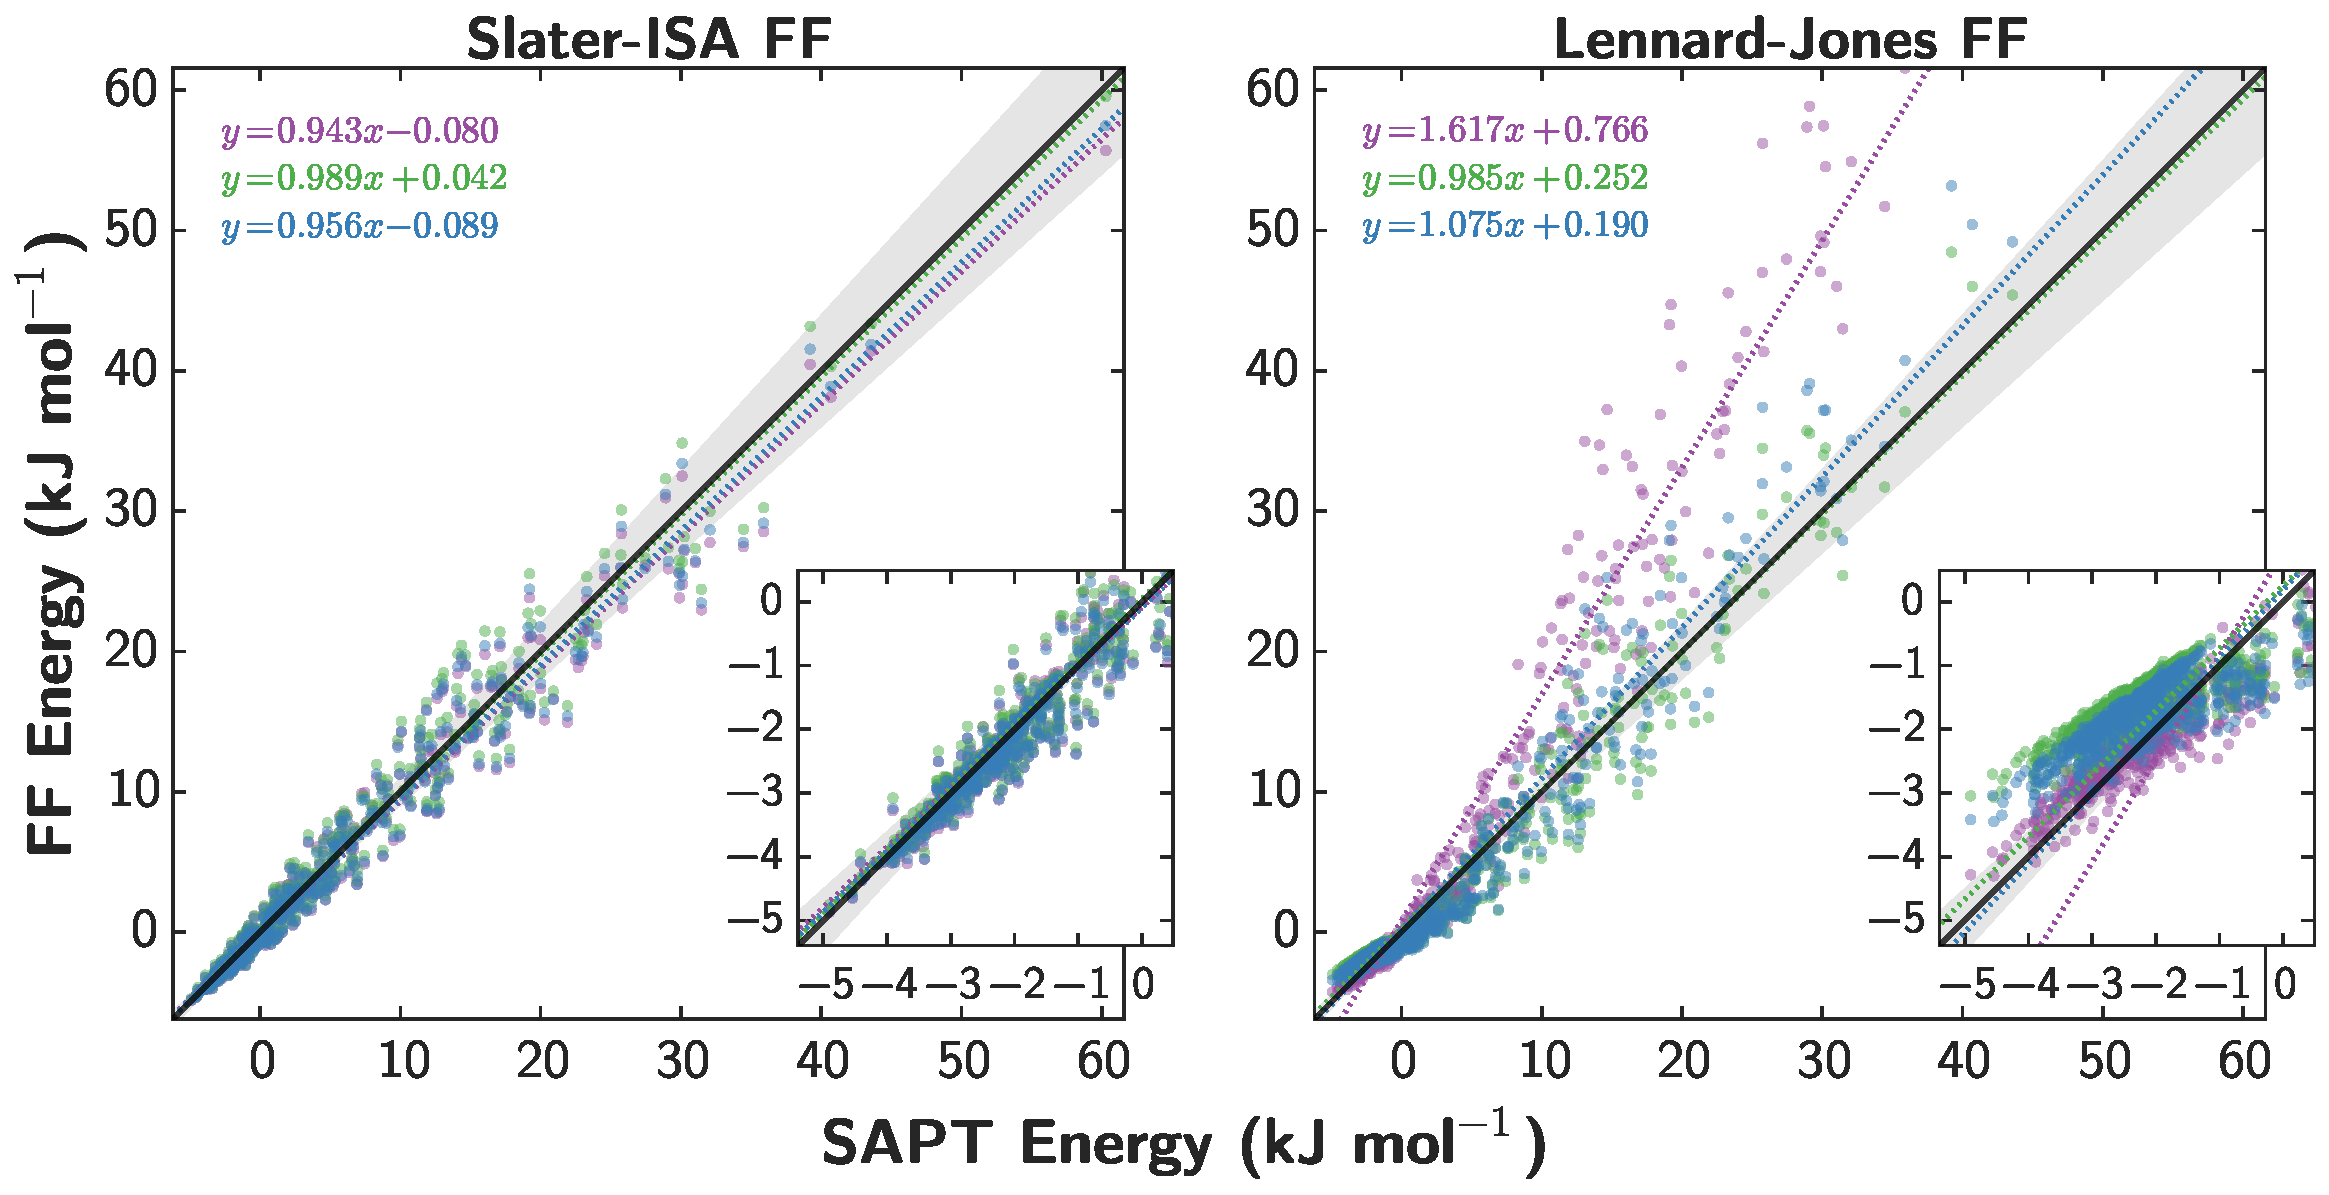
\includegraphics[width=0.8\textwidth]{isotropic/si/compare_lj_ethane_ethane_scatter.pdf}
%%     \vspace{10 mm}
%%     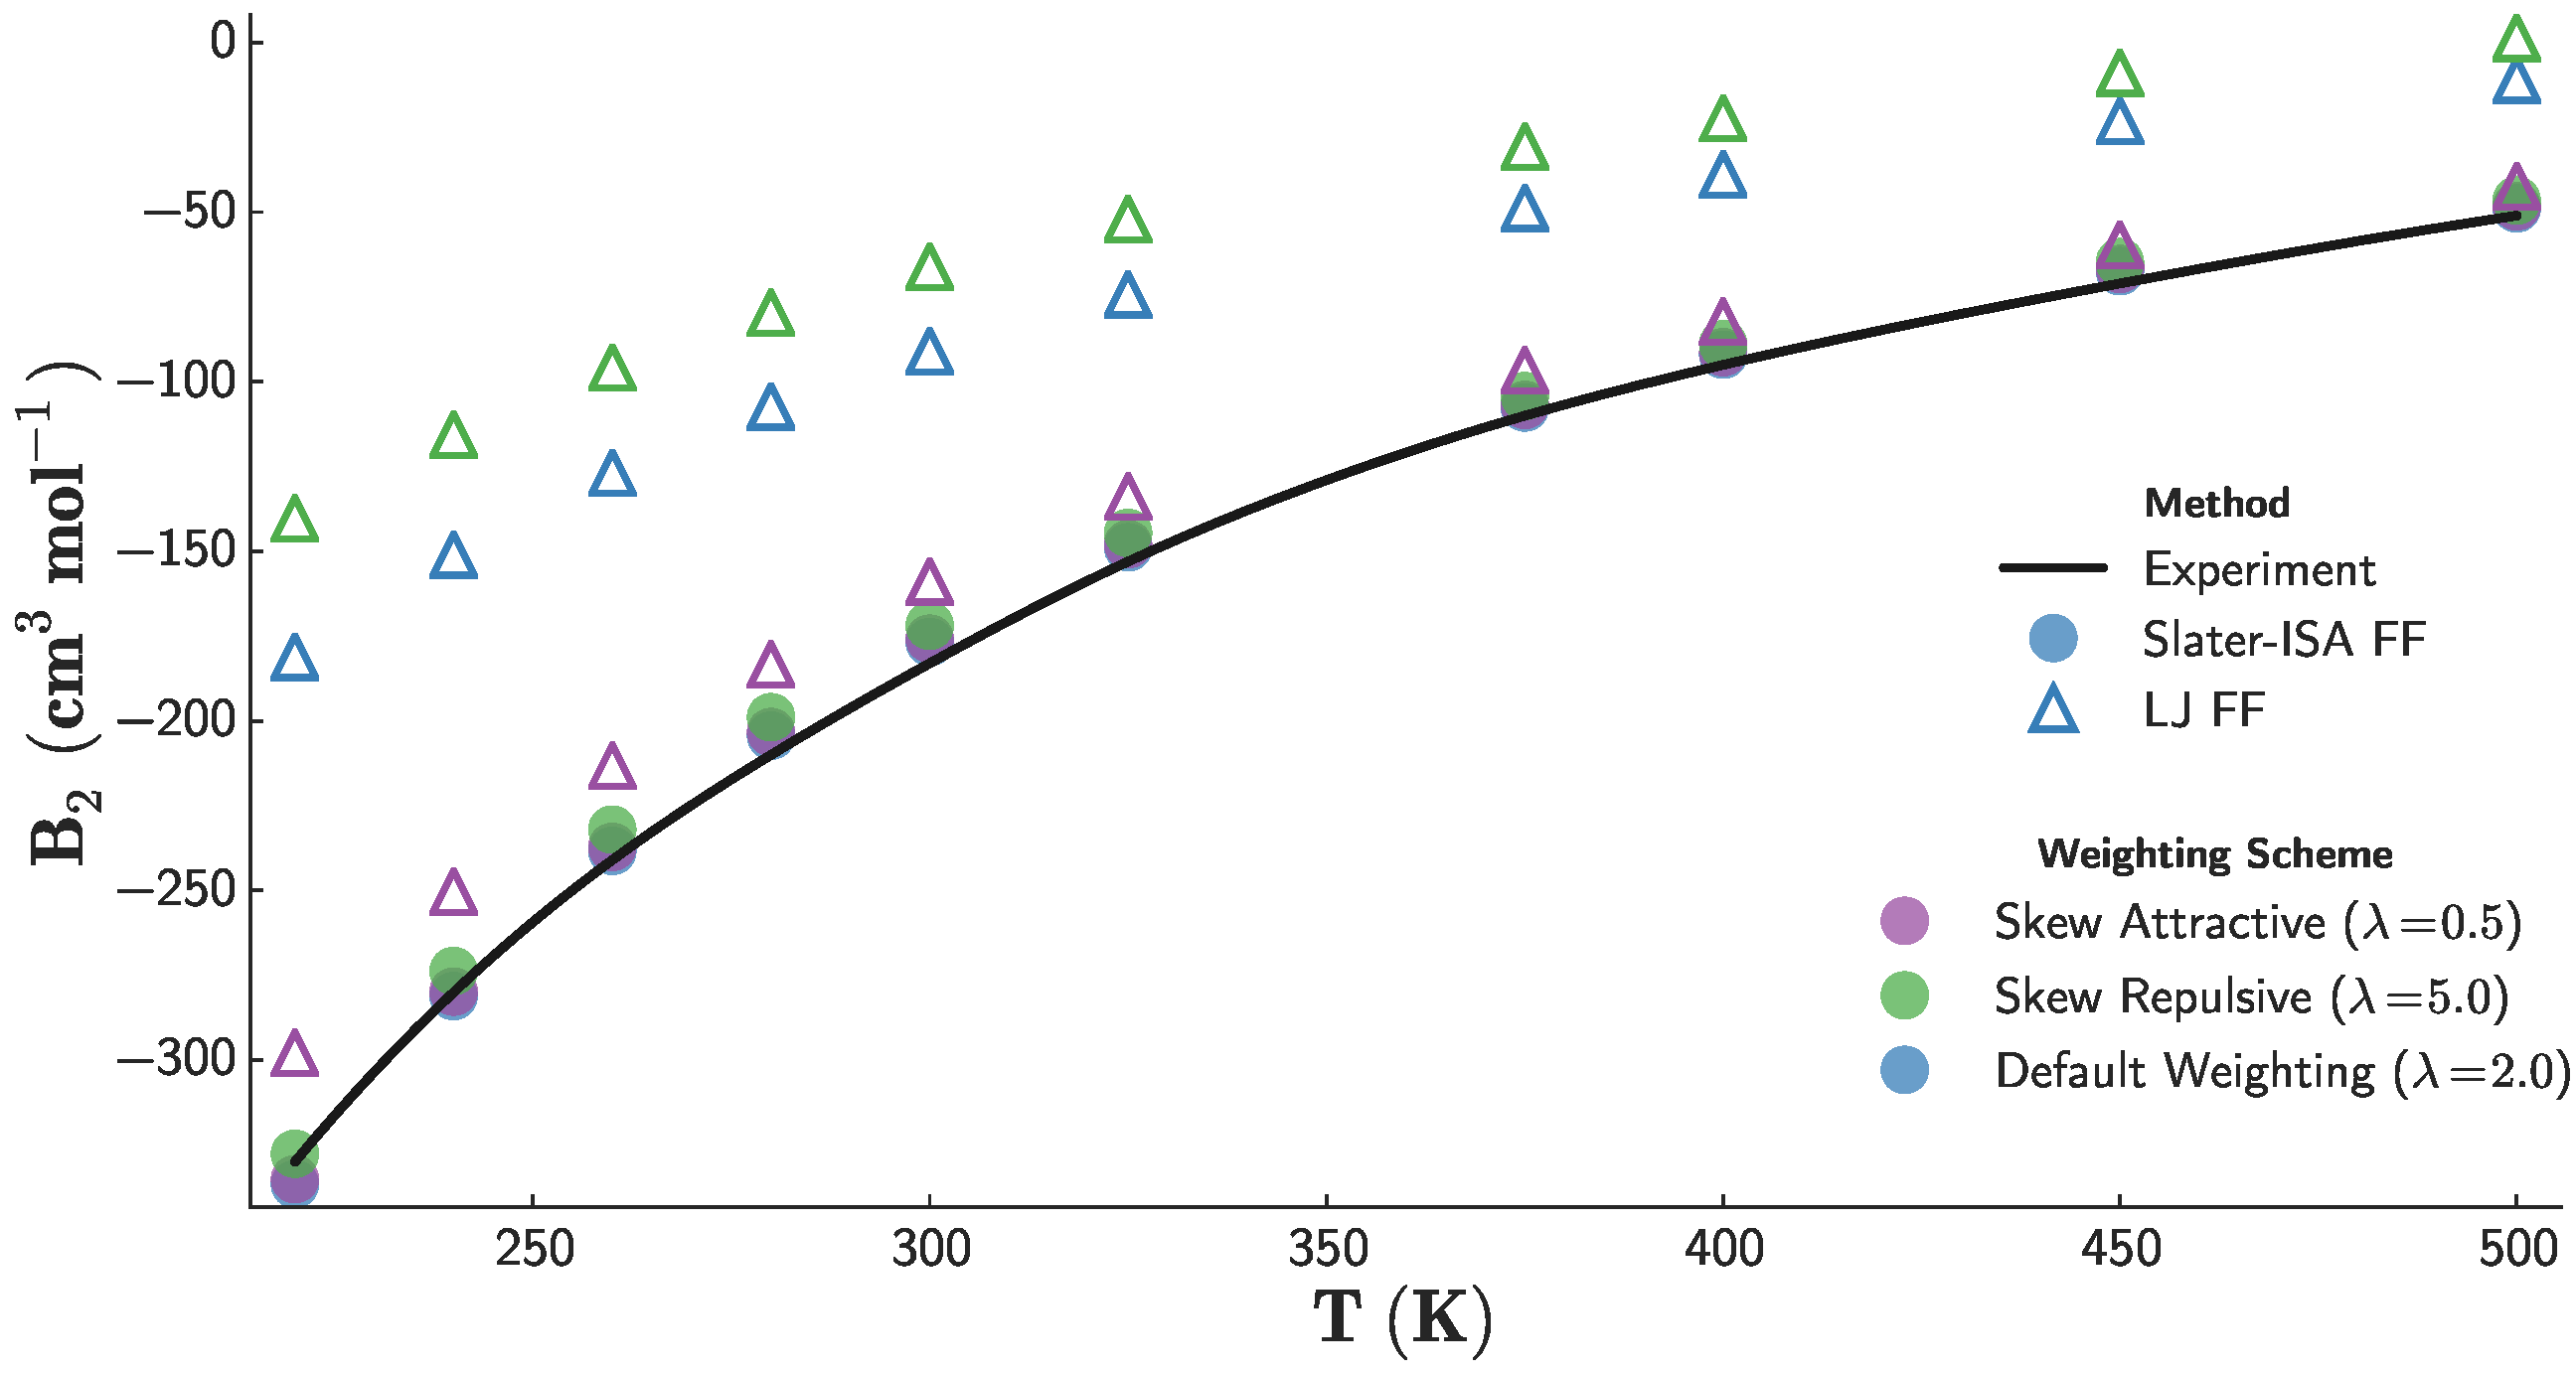
\includegraphics[width=0.8\textwidth]{isotropic/si/weighted_ethane_2nd_virial_lj.pdf}
%%     \caption[foo]{
%%         Comparison of the \isaffold and the \ljff in terms of sensitivity to the
%%         weighting function employed in parameter optimization for the ethane
%%         dimer. Three weighting functions, $\lambda = 0.5$ (purple), $\lambda = 2.0$
%%         (blue), and $\lambda = 5.0$ (green) are shown, with higher $\lambda$ values
%%         indicating more weighting of repulsive configurations.
%% 
%%         (top) Total interaction energies for the \isaffold (left) and the \ljff (right)
%%         indicating the accuracy of each force field with respect to \saptpbeo benchmark
%%         energies.  The diagonal line (black) indicates perfect agreement between
%%         reference energies and each force field, while shaded grey areas represent
%%         points within $\pm 10\%$ agreement of the benchmark.  To guide the eye, a line
%%         of best fit (dotted line) has been computed for each force field and for each
%%         weighting function.
%%               
%%         (bottom) Computed 2$^\text{nd}$ virial coefficients for argon. Data for
%%         the \isaffold and the \saptff are depicted using open circles and shaded squares,
%%         respectively; coloration for the different weighting functions is as above.
%%         Experimental data from \citeauthor{Dymond1980} (black line) is also shown.
%%       %ASK: Do we actually cite Dymond and Smith for this, since it's a compiled
%%       %work, or do I need to try and dig up the original experimentallist?
%%     }
%%     \label{fig:ar-weighting}
%% 
%%     \end{figure}
%%     %%%%%%%% Weighting Function Tests %%%%%%%
%% \end{section}
%% 
%% 
%% \pagebreak
%% \scriptsize
%% %% \begin{table}
\centering
\renewcommand\arraystretch{1.1}
\begin{longtable}{@{}ccccccc@{}}
\caption{Fitted values for Bij for a variety of element pairs. All values are
given in atomic units, except for RMS errors, which are a unitless normalized
overlap.} \label{tab:all_bij_exponents} \\

\hline
\toprule
$i$ &  $j$  &        $B_i$     &     $B_j$     &    $B_{ij}$   &      RMSE   & MAPE   \\    
\midrule
\endfirsthead

\multicolumn{6}{c}%
{{\bfseries \tablename\ \thetable{} -- continued from previous page}} \\
\hline
\toprule
$i$ &  $j$  &        $B_i$     &     $B_j$     &    $B_{ij}$   &      RMSE  & MAPE    \\    
\midrule
\endhead

\bottomrule
\hline
\endfoot

H  &  He    &     1.99946394   &   2.68859863  &    2.31740474 &  0.00044277657  &  0.882930\\
H  &  Li    &     1.99946394   &   1.25901971  &    1.59404909 &  0.00064319203  &  1.106033\\
H  &  Be    &     1.99946394   &   1.65554322  &    1.82052039 &  0.00012960395  &  0.217206\\
H  &  B     &     1.99946394   &   1.56191136  &    1.76768239 &  0.00022762336  &  0.498291\\
H  &  C     &     1.99946394   &   1.81946896  &    1.90742066 &  3.6383389e-05  &  0.074853\\
H  &  N     &     1.99946394   &   2.06711073  &    2.03302187 &  4.9406068e-06  &  0.009742\\
H  &  O     &     1.99946394   &   2.00091172  &    2.00019722 &  9.9506754e-08  &  0.000183\\
H  &  F     &     1.99946394   &   2.26322976  &    2.12730789 &  7.0666272e-05  &  0.137228\\
H  &  Ne    &     1.99946394   &   2.51791099  &    2.24270366 &  0.00026455338  &  0.578093\\
H  &  Na    &     1.99946394   &   1.22917354  &    1.57023314 &  0.00074952732  &  1.738728\\
H  &  Mg    &     1.99946394   &   1.49931366  &    1.73354253 &   0.0002881065  &  0.529739\\
H  &  Al    &     1.99946394   &   1.32657183  &    1.63349076 &  0.00053449852  &  0.976877\\
H  &  Si    &     1.99946394   &   1.54808130  &    1.75910683 &  0.00024917876  &  0.617006\\
H  &  P     &     1.99946394   &   1.75585679  &    1.87377325 &  6.8182489e-05  &  0.148197\\
H  &  S     &     1.99946394   &   1.74521745  &    1.86810662 &  7.4332699e-05  &  0.160880\\
H  &  Cl    &     1.99946394   &   1.95253790  &    1.97586738 &  2.5436846e-06  &  0.005705\\
H  &  Ar    &     1.99946394   &   2.15249556  &    2.07440522 &  2.5899665e-05  &  0.068500\\
H  &  Br    &     1.99946394   &   1.86365053  &    1.93033996 &   2.112332e-05  &  0.048965\\
H  &  I     &     1.99946394   &   1.75289066  &    1.87194355 &  7.1892596e-05  &  0.178949\\
He &  Li    &     2.68859863   &   1.25901971  &    1.83579487 &   0.0020586815  &  4.802329\\
He &  Be    &     2.68859863   &   1.65554322  &    2.10352673 &   0.0010603604  &  2.573450\\
He &  B     &     2.68859863   &   1.56191136  &    2.03442611 &     0.00129508  &  3.918107\\
He &  C     &     2.68859863   &   1.81946896  &    2.20238570 &  0.00075763278  &  2.262394\\
He &  N     &     2.68859863   &   2.06711073  &    2.35237454 &   0.0003780889  &  1.127971\\
He &  O     &     2.68859863   &   2.00091172  &    2.31393264 &  0.00046386026  &  1.314845\\
He &  F     &     2.68859863   &   2.26322976  &    2.46423057 &   0.0001731239  &  0.522637\\
He &  Ne    &     2.68859863   &   2.51791099  &    2.60133215 &  2.7253815e-05  &  0.094670\\
He &  Na    &     2.68859863   &   1.22917354  &    1.79792813 &   0.0021797532  &  6.560866\\
He &  Mg    &     2.68859863   &   1.49931366  &    1.99849093 &   0.0014277708  &  3.668547\\
He &  Al    &     2.68859863   &   1.32657183  &    1.88040364 &   0.0018777097  &  4.668027\\
He &  Si    &     2.68859863   &   1.54808130  &    2.02089719 &    0.001334628  &  4.489483\\
He &  P     &     2.68859863   &   1.75585679  &    2.16119527 &  0.00087958401  &  2.730605\\
He &  S     &     2.68859863   &   1.74521745  &    2.15451616 &  0.00090006465  &  2.778815\\
He &  Cl    &     2.68859863   &   1.95253790  &    2.28271739 &  0.00054130424  &  1.785225\\
He &  Ar    &     2.68859863   &   2.15249556  &    2.39953728 &  0.00028412395  &  1.122892\\
He &  Br    &     2.68859863   &   1.86365053  &    2.22767127 &  0.00068597032  &  2.295912\\
He &  I     &     2.68859863   &   1.75289066  &    2.15618545 &      0.0008917  &  3.122234\\
Li &  Be    &     1.25901971   &   1.65554322  &    1.44552618 &  0.00021566494  &  0.459735\\
Li &  B     &     1.25901971   &   1.56191136  &    1.40276036 &  0.00013669061  &  0.361720\\
Li &  C     &     1.25901971   &   1.81946896  &    1.51465672 &  0.00042489929  &  1.056460\\
Li &  N     &     1.25901971   &   2.06711073  &    1.61476325 &  0.00080816618  &  1.922263\\
Li &  O     &     1.25901971   &   2.00091172  &    1.58945583 &  0.00069142836  &  1.593136\\
Li &  F     &     1.25901971   &   2.26322976  &    1.68919749 &   0.0011668895  &  2.718352\\
Li &  Ne    &     1.25901971   &   2.51791099  &    1.77555429 &   0.0017026265  &  4.273871\\
Li &  Na    &     1.25901971   &   1.22917354  &    1.24402068 &  1.5533688e-06  &  0.004373\\
Li &  Mg    &     1.25901971   &   1.49931366  &    1.37457277 &  8.4735331e-05  &  0.195212\\
Li &  Al    &     1.25901971   &   1.32657183  &    1.29242716 &  7.1019258e-06  &  0.016335\\
Li &  Si    &     1.25901971   &   1.54808130  &    1.39618447 &  0.00012793291  &  0.374607\\
Li &  P     &     1.25901971   &   1.75585679  &    1.48750641 &  0.00034426274  &  0.896554\\
Li &  S     &     1.25901971   &   1.74521745  &    1.48302253 &  0.00033062213  &  0.858653\\
Li &  Cl    &     1.25901971   &   1.95253790  &    1.56786800 &  0.00063028803  &  1.664314\\
Li &  Ar    &     1.25901971   &   2.15249556  &    1.64158799 &  0.00099309611  &  2.932927\\
Li &  Br    &     1.25901971   &   1.86365053  &    1.53172970 &  0.00049638053  &  1.350986\\
Li &  I     &     1.25901971   &   1.75289066  &    1.48527643 &  0.00034799167  &  1.009017\\
Be &  B     &     1.65554322   &   1.56191136  &    1.60804807 &  1.1972231e-05  &  0.031893\\
Be &  C     &     1.65554322   &   1.81946896  &    1.73554580 &  3.3972736e-05  &  0.085743\\
Be &  N     &     1.65554322   &   2.06711073  &    1.84956812 &   0.0001992019  &  0.484038\\
Be &  O     &     1.65554322   &   2.00091172  &    1.82001716 &  0.00014155775  &  0.330806\\
Be &  F     &     1.65554322   &   2.26322976  &    1.93457449 &  0.00041123838  &  0.983581\\
Be &  Ne    &     1.65554322   &   2.51791099  &    2.03628351 &  0.00078343308  &  2.059895\\
Be &  Na    &     1.65554322   &   1.22917354  &    1.42686604 &  0.00026737271  &  0.745777\\
Be &  Mg    &     1.65554322   &   1.49931366  &    1.57563633 &  3.2478195e-05  &  0.074055\\
Be &  Al    &     1.65554322   &   1.32657183  &    1.48286105 &  0.00014866739  &  0.335525\\
Be &  Si    &     1.65554322   &   1.54808130  &    1.60086762 &   1.615263e-05  &  0.048036\\
Be &  P     &     1.65554322   &   1.75585679  &    1.70494709 &  1.3101092e-05  &  0.034696\\
Be &  S     &     1.65554322   &   1.74521745  &    1.69977980 &  1.0504303e-05  &  0.027715\\
Be &  Cl    &     1.65554322   &   1.95253790  &    1.79750301 &  0.00010922498  &  0.297117\\
Be &  Ar    &     1.65554322   &   2.15249556  &    1.88512628 &  0.00029576275  &  0.923403\\
Be &  Br    &     1.65554322   &   1.86365053  &    1.75630627 &  5.5219463e-05  &  0.154638\\
Be &  I     &     1.65554322   &   1.75289066  &    1.70346914 &  1.2636043e-05  &  0.037713\\
B  &  C     &     1.56191136   &   1.81946896  &    1.68526246 &   8.896852e-05  &  0.279460\\
B  &  N     &     1.56191136   &   2.06711073  &    1.79465183 &  0.00031660316  &  0.962841\\
B  &  O     &     1.56191136   &   2.00091172  &    1.76649990 &  0.00024246047  &  0.712022\\
B  &  F     &     1.56191136   &   2.26322976  &    1.87554766 &  0.00057369687  &  1.719903\\
B  &  Ne    &     1.56191136   &   2.51791099  &    1.97105959 &  0.00099084843  &  3.222525\\
B  &  Na    &     1.56191136   &   1.22917354  &    1.38509763 &  0.00017473338  &  0.590078\\
B  &  Mg    &     1.56191136   &   1.49931366  &    1.53029477 &  5.6807294e-06  &  0.016154\\
B  &  Al    &     1.56191136   &   1.32657183  &    1.43954012 &  8.2359665e-05  &  0.230371\\
B  &  Si    &     1.56191136   &   1.54808130  &    1.55498504 &  3.4970147e-07  &  0.001260\\
B  &  P     &     1.56191136   &   1.75585679  &    1.65571982 &  5.1764703e-05  &  0.169673\\
B  &  S     &     1.56191136   &   1.74521745  &    1.65073751 &  4.6359978e-05  &  0.151426\\
B  &  Cl    &     1.56191136   &   1.95253790  &    1.74462228 &  0.00019882685  &  0.668654\\
B  &  Ar    &     1.56191136   &   2.15249556  &    1.82774537 &  0.00043254436  &  1.644894\\
B  &  Br    &     1.56191136   &   1.86365053  &    1.70507656 &  0.00012232055  &  0.422076\\
B  &  I     &     1.56191136   &   1.75289066  &    1.65418604 &  5.1089297e-05  &  0.186574\\
C  &  N     &     1.81946896   &   2.06711073  &    1.93878424 &  7.2588349e-05  &  0.213967\\
C  &  O     &     1.81946896   &   2.00091172  &    1.90779431 &  3.9381872e-05  &  0.111509\\
C  &  F     &     1.81946896   &   2.26322976  &    2.02729827 &  0.00022128603  &  0.646349\\
C  &  Ne    &     1.81946896   &   2.51791099  &    2.13356824 &  0.00051712548  &  1.665041\\
C  &  Na    &     1.81946896   &   1.22917354  &    1.49359005 &  0.00049650546  &  1.590315\\
C  &  Mg    &     1.81946896   &   1.49931366  &    1.65145683 &  0.00013523926  &  0.364498\\
C  &  Al    &     1.81946896   &   1.32657183  &    1.55375705 &  0.00032909645  &  0.868090\\
C  &  Si    &     1.81946896   &   1.54808130  &    1.67745495 &  0.00010070423  &  0.351275\\
C  &  P     &     1.81946896   &   1.75585679  &    1.78734889 &  5.2847945e-06  &  0.016690\\
C  &  S     &     1.81946896   &   1.74521745  &    1.78191233 &  7.1848878e-06  &  0.022600\\
C  &  Cl    &     1.81946896   &   1.95253790  &    1.88462580 &  2.1955555e-05  &  0.071858\\
C  &  Ar    &     1.81946896   &   2.15249556  &    1.97704725 &   0.0001323859  &  0.499304\\
C  &  Br    &     1.81946896   &   1.86365053  &    1.84141110 &  2.5492317e-06  &  0.008538\\
C  &  I     &     1.81946896   &   1.75289066  &    1.78581710 &  5.8824253e-06  &  0.020847\\
N  &  O     &     2.06711073   &   2.00091172  &    2.03371451 &   5.041231e-06  &  0.013929\\
N  &  F     &     2.06711073   &   2.26322976  &    2.16254689 &    4.15042e-05  &  0.119485\\
N  &  Ne    &     2.06711073   &   2.51791099  &    2.27840189 &  0.00020910088  &  0.673215\\
N  &  Na    &     2.06711073   &   1.22917354  &    1.58958212 &  0.00090815621  &  2.796799\\
N  &  Mg    &     2.06711073   &   1.49931366  &    1.75954426 &  0.00039310972  &  1.019328\\
N  &  Al    &     2.06711073   &   1.32657183  &    1.65570661 &  0.00068105488  &  1.722447\\
N  &  Si    &     2.06711073   &   1.54808130  &    1.78559923 &  0.00033982883  &  1.150687\\
N  &  P     &     2.06711073   &   1.75585679  &    1.90415582 &  0.00011669305  &  0.359120\\
N  &  S     &     2.06711073   &   1.74521745  &    1.89832775 &  0.00012494822  &  0.382742\\
N  &  Cl    &     2.06711073   &   1.95253790  &    2.00885032 &  1.5404889e-05  &  0.049510\\
N  &  Ar    &     2.06711073   &   2.15249556  &    2.10924579 &  8.3837241e-06  &  0.031515\\
N  &  Br    &     2.06711073   &   1.86365053  &    1.96222048 &   4.938888e-05  &  0.162281\\
N  &  I     &     2.06711073   &   1.75289066  &    1.90214169 &  0.00012093134  &  0.419448\\
O  &  F     &     2.00091172   &   2.26322976  &    2.12742019 &  7.4513608e-05  &  0.204667\\
O  &  Ne    &     2.00091172   &   2.51791099  &    2.24105845 &  0.00027602296  &  0.845765\\
O  &  Na    &     2.00091172   &   1.22917354  &    1.56546880 &  0.00078625246  &  2.354990\\
O  &  Mg    &     2.00091172   &   1.49931366  &    1.73176044 &  0.00031061975  &  0.777382\\
O  &  Al    &     2.00091172   &   1.32657183  &    1.62980355 &  0.00057319586  &  1.403523\\
O  &  Si    &     2.00091172   &   1.54808130  &    1.75782981 &  0.00026287602  &  0.860753\\
O  &  P     &     2.00091172   &   1.75585679  &    1.87387688 &  7.3175089e-05  &  0.216650\\
O  &  S     &     2.00091172   &   1.74521745  &    1.86815729 &  7.9760452e-05  &  0.235090\\
O  &  Cl    &     2.00091172   &   1.95253790  &    1.97655937 &  2.8387158e-06  &  0.008742\\
O  &  Ar    &     2.00091172   &   2.15249556  &    2.07494432 &  2.6479263e-05  &  0.095246\\
O  &  Br    &     2.00091172   &   1.86365053  &    1.93085797 &  2.2760392e-05  &  0.071837\\
O  &  I     &     2.00091172   &   1.75289066  &    1.87203787 &  7.6356395e-05  &  0.255064\\
F  &  Ne    &     2.26322976   &   2.51791099  &    2.38617019 &  6.4967098e-05  &  0.211473\\
F  &  Na    &     2.26322976   &   1.22917354  &    1.66029149 &   0.0012830926  &  3.875179\\
F  &  Mg    &     2.26322976   &   1.49931366  &    1.83986590 &  0.00066962961  &  1.706670\\
F  &  Al    &     2.26322976   &   1.32657183  &    1.73140874 &   0.0010196712  &  2.528620\\
F  &  Si    &     2.26322976   &   1.54808130  &    1.86526151 &  0.00060490347  &  2.020578\\
F  &  P     &     2.26322976   &   1.75585679  &    1.99065290 &  0.00029360355  &  0.894671\\
F  &  S     &     2.26322976   &   1.74521745  &    1.98453998 &  0.00030630021  &  0.928727\\
F  &  Cl    &     2.26322976   &   1.95253790  &    2.10087150 &  0.00010755539  &  0.344316\\
F  &  Ar    &     2.26322976   &   2.15249556  &    2.20694293 &  1.3485721e-05  &  0.050987\\
F  &  Br    &     2.26322976   &   1.86365053  &    2.05158173 &  0.00018081195  &  0.590554\\
F  &  I     &     2.26322976   &   1.75289066  &    1.98794200 &  0.00030142935  &  1.036990\\
Ne &  Na    &     2.51791099   &   1.22917354  &    1.74146757 &   0.0018171227  &  5.842510\\
Ne &  Mg    &     2.51791099   &   1.49931366  &    1.93474540 &   0.0011134419  &  3.086201\\
Ne &  Al    &     2.51791099   &   1.32657183  &    1.81962923 &    0.001531155  &  4.095464\\
Ne &  Si    &     2.51791099   &   1.54808130  &    1.95888870 &   0.0010266525  &  3.702217\\
Ne &  P     &     2.51791099   &   1.75585679  &    2.09400464 &  0.00062146304  &  2.076964\\
Ne &  S     &     2.51791099   &   1.74521745  &    2.08750459 &  0.00063928574  &  2.124924\\
Ne &  Cl    &     2.51791099   &   1.95253790  &    2.21174754 &  0.00033656173  &  1.193911\\
Ne &  Ar    &     2.51791099   &   2.15249556  &    2.32497739 &  0.00013843693  &  0.584890\\
Ne &  Br    &     2.51791099   &   1.86365053  &    2.15873868 &      0.0004557  &  1.639505\\
Ne &  I     &     2.51791099   &   1.75289066  &    2.09004196 &  0.00063134274  &  2.372214\\
Na &  Mg    &     1.22917354   &   1.49931366  &    1.35766104 &  0.00011473889  &  0.341738\\
Na &  Al    &     1.22917354   &   1.32657183  &    1.27699602 &  1.5803838e-05  &  0.046721\\
Na &  Si    &     1.22917354   &   1.54808130  &    1.37861851 &  0.00016394224  &  0.606312\\
Na &  P     &     1.22917354   &   1.75585679  &    1.46734689 &  0.00040724885  &  1.358887\\
Na &  S     &     1.22917354   &   1.74521745  &    1.46301699 &  0.00039233117  &  1.305796\\
Na &  Cl    &     1.22917354   &   1.95253790  &    1.54462666 &  0.00071489747  &  2.415615\\
Na &  Ar    &     1.22917354   &   2.15249556  &    1.61475657 &   0.0010865392  &  4.048855\\
Na &  Br    &     1.22917354   &   1.86365053  &    1.50991318 &  0.00057095415  &  1.982122\\
Na &  I     &     1.22917354   &   1.75289066  &    1.46507909 &  0.00040898615  &  1.502211\\
Mg &  Al    &     1.49931366   &   1.32657183  &    1.41054381 &  4.3759475e-05  &  0.106460\\
Mg &  Si    &     1.49931366   &   1.54808130  &    1.52349731 &  3.5595022e-06  &  0.011234\\
Mg &  P     &     1.49931366   &   1.75585679  &    1.62233525 &  8.9250076e-05  &  0.251892\\
Mg &  S     &     1.49931366   &   1.74521745  &    1.61744114 &  8.2197924e-05  &  0.231214\\
Mg &  Cl    &     1.49931366   &   1.95253790  &    1.70986111 &  0.00026403315  &  0.761802\\
Mg &  Ar    &     1.49931366   &   2.15249556  &    1.79169870 &  0.00052474149  &  1.715332\\
Mg &  Br    &     1.49931366   &   1.86365053  &    1.67083027 &  0.00017608345  &  0.522795\\
Mg &  I     &     1.49931366   &   1.75289066  &    1.62071071 &  8.9123446e-05  &  0.281480\\
Al &  Si    &     1.32657183   &   1.54808130  &    1.43295795 &  7.4878405e-05  &  0.231698\\
Al &  P     &     1.32657183   &   1.75585679  &    1.52615042 &  0.00025709446  &  0.709802\\
Al &  S     &     1.32657183   &   1.74521745  &    1.52156219 &  0.00024519155  &  0.674974\\
Al &  Cl    &     1.32657183   &   1.95253790  &    1.60826232 &  0.00051441718  &  1.443233\\
Al &  Ar    &     1.32657183   &   2.15249556  &    1.68396084 &   0.0008502512  &  2.673094\\
Al &  Br    &     1.32657183   &   1.86365053  &    1.57145555 &  0.00039199648  &  1.132597\\
Al &  I     &     1.32657183   &   1.75289066  &    1.52414100 &  0.00025909364  &  0.796534\\
Si &  P     &     1.54808130   &   1.75585679  &    1.64816385 &  6.0537472e-05  &  0.219836\\
Si &  S     &     1.54808130   &   1.74521745  &    1.64322319 &  5.4646042e-05  &  0.197756\\
Si &  Cl    &     1.54808130   &   1.95253790  &    1.73616531 &  0.00021653004  &  0.806893\\
Si &  Ar    &     1.54808130   &   2.15249556  &    1.81809419 &  0.00045725342  &  1.916727\\
Si &  Br    &     1.54808130   &   1.86365053  &    1.69704848 &  0.00013598439  &  0.519161\\
Si &  I     &     1.54808130   &   1.75289066  &    1.64662155 &   5.971014e-05  &  0.240522\\
P  &  S     &     1.75585679   &   1.74521745  &    1.75053498 &  2.2383111e-07  &  0.000726\\
P  &  Cl    &     1.75585679   &   1.95253790  &    1.85109487 &  4.8767404e-05  &  0.166222\\
P  &  Ar    &     1.75585679   &   2.15249556  &    1.94118289 &  0.00019034099  &  0.743408\\
P  &  Br    &     1.75585679   &   1.86365053  &    1.80880477 &  1.5089803e-05  &  0.052666\\
P  &  I     &     1.75585679   &   1.75289066  &    1.75438024 &  8.3311914e-08  &  0.000297\\
S  &  Cl    &     1.74521745   &   1.95253790  &    1.84542979 &  5.4259063e-05  &  0.184109\\
S  &  Ar    &     1.74521745   &   2.15249556  &    1.93516069 &  0.00020092813  &  0.780785\\
S  &  Br    &     1.74521745   &   1.86365053  &    1.80328668 &  1.8231579e-05  &  0.063360\\
S  &  I     &     1.74521745   &   1.75289066  &    1.74905593 &  1.5042953e-07  &  0.000542\\
Cl &  Ar    &     1.95253790   &   2.15249556  &    2.04925011 &  4.7026489e-05  &  0.193758\\
Cl &  Br    &     1.95253790   &   1.86365053  &    1.90746100 &  9.8799774e-06  &  0.035850\\
Cl &  I     &     1.95253790   &   1.75289066  &    1.84935929 &  5.0999292e-05  &  0.194814\\
Ar &  Br    &     2.15249556   &   1.86365053  &    2.00111347 &  9.9755127e-05  &  0.417023\\
Ar &  I     &     2.15249556   &   1.75289066  &    1.93889388 &  0.00019497498  &  0.849907\\
Br &  I     &     1.86365053   &   1.75289066  &    1.80721936 &  1.6163908e-05  &  0.063089\\
%\bottomrule
\end{longtable}
%% \end{table}

%% \normalsize
%% 
%% %% \end{section}
%% 
%% 
%% \singlespacing
%% 
%% \renewcommand{\baselinestretch}{1}
%% 
%% \bibliographystyle{achemso}
%% \bibliography{/Users/Mary/Documents/library}
%% %\bibliography{rp_extras}
%% 
%% 
%% \end{document}
 
\end{subappendices}


\end{chapter}

\glsresetall 
\begin{chapter}{\mastiff: A General Approach for Incorporating Atomic-level
Anisotropy in Ab Initio Force Fields}
\label{ch:mastiff}

%%%%%%%%%%%%%%%%%%%%%%%%%%%%%%%%% Introduction %%%%%%%%%%%%%%%%%%%%%%%%%%%%%%%%%%%%
\begin{section}{Introduction}
\label{sec:intro}

%auto-ignore
Classical molecular simulation is a standard tool for
interpreting and predicting the chemistry of an incredible host of systems ranging
from simple liquids to complex materials and biomolecules. Such simulations
always require, as input, a mathematical description of the
system's potential energy surface (PES). In principle, the
PES for most chemical systems can accurately be determined 
from one of several high-level electronic structure methods;
\cite{Rezac2016,Chalasinski2000,Jan2016}
nevertheless, these calculations are currently too expensive to use
in simulations of large systems and/or long timescales. 
\cite{Hassanali2014}
Consequently, most routine
molecular simulation today is performed with the aid of force fields:
computationally-inexpensive, parameterized mathematical expressions that
approximate the exact PES. Because the accuracy and predictive capabilities of
molecular simulation are directly tied to the underlying force
field, one of the central challenges of molecular
simulation is the development of highly accurate force fields. For ab initio
force field development, this accuracy is 
principally defined by a force field's fidelity to the underlying exact PES. 

As of now, several common
shortcomings\cite{Zgarbova2010} inhibit the accuracy and predictive capabilities of
standard ab initio force fields, and these limitations must be systematically addressed
in order to generate improved, `next-generation' force fields. One important
shortcoming, which will be the focus of this Chapter, is the so-called
`sum-of-spheres' approximation,\cite{Stone1988} in which it is assumed that the
non-bonding interactions between molecules can be treated as a superposition
of interactions between pairs of spherically-symmetric atoms.
Put differently, the sum-of-spheres, or `isotropic atom-atom', approximation assumes that the 
exact PES, \etot (which depends
both on the center of mass distance $R$ and relative orientation $\Omega$ between molecules),
can be modeled as
\begin{align}
\label{eq:sos_approx}
\etot(R,\Omega) \approx \sum\limits_{ij} f(r_{ij}) \equiv \vtot,
\end{align}
where the above sum runs over all
non-bonded pairs of atoms $i$ and $j$ with interatomic separation $r_{ij}$,
and $f(r_{ij})$ is an arbitrary, distance-dependent function that defines the pairwise
interaction.
Here and throughout, we use $E$ to denote the true PES, and $V$ to denote the
corresponding model/force field prediction. 
With some exceptions (vida infra), nearly all standard intermolecular force
fields ---
ranging from the popular ``Lennard-Jones plus point charges'' model to more complex
functional forms\cite{Schmidt2015}
---
explicitly make use of the isotropic atom-atom model.

Notwithstanding the popularity of the model, there is good experimental and
theoretical evidence to suggest that the sum-of-spheres approximation does not
hold in practice.\cite{stone2013theory,Stone1988,Price2000} 
Importantly, and as we argue in
\cref{sec:results}, models which include anisotropic (multipolar) electrostatics, but
otherwise employ the sum-of-spheres approximation, are an improved but
\emph{still incomplete} model for
describing the atomic-level anisotropy of intermolecular interactions.
Experimentally, it has long been known that 
atom-in-molecule charge densities, as determined from x-ray diffraction, can exhibit significant
non-spherical features, such as with lone pair or $\pi$ electron
densities.\cite{Coppens1979} Furthermore, statistical analyses of the
Cambridge Structural Database 
% cite this? is it the cambridge structural database or crystal structure
% database?
have shown that the the van der Waals radii of atoms-in-molecules (as measured
from interatomic closest contact distances)
are not isotropically
distributed, but rather show strong orientation dependencies, particularly for
halogens and other heteroatoms.
\cite{Bondi1964,Nyburg1985,Batsanov2001,Auffinger2004,Lommerse1996,Eramian2013} 
These experimental studies are corroborated by a significant body of
theoretical research on both the anisotropy of the atomic van der Waals radii
as well as the non-spherical features of the atomic charge densities themselves.
\cite{Wheatley2012,Kramer2014,Lommerse1996, Badenhoop1997a,Kim2014b,Bankiewicz2012}
These studies suggest
that the sum-of-spheres approximation is an insufficiently
flexible model for the subset of intermolecular interactions that arise from
atomically non-spherical charge
densities, and may help explain known difficulties in generating accurate
isotropic atom-atom force fields for such important chemical interactions as 
$\pi$-interactions,\cite{Chessari2002,Sponer2013,Sherrill2009}
$\sigma$-bonding,\cite{Bartocci2015,Rendine2011,Politzer2008}
and hydrogen bonding,\cite{Cisneros2016a}
(see \citen{Cardamone2014} and references therein).

Motivated by these observations,
a small but important  body of work has been
devoted to directly addressing the limitations of the isotropic atom-atom
model in the context of `next-generation' force field development. As will be discussed in
detail below (see \cref{sec:prior_work}), the general conclusion from these
studies is that many components of intermolecular interactions
(specifically electrostatics, exchange-repulsion, induction, and
dispersion)
can be more accurately modeled by functional forms that go beyond the
sum-of-spheres approximation.
\cite{Price2000,Hagler2015,Ren2003}
While few intermolecular potentials (and virtually no standard force fields
amenable to routine molecular simulation) explicitly account for atomic-level anisotropy
for each component of intermolecular interactions, several recent standard force fields
have incorporated atomic-level anisotropy into their description of 
long-range electrostatics.\cite{Cardamone2014} Some of these potentials
(notably AMOEBA\cite{Ponder2010,Ren2003,Shi2013} and some water
potentials\cite{Cisneros2016a,Cardamone2014}) 
are already employed in large-scale molecular simulation, often with very
encouraging success.\cite{Cardamone2014}
Furthermore, others have shown that anisotropic potentials (some of which additionally
model the anisotropy of exchange-repulsion
and/or dispersion) lead to significant improvements in predicting 
molecular crystal structures.
\cite{Cardamone2014,Price2010a,Day1999,Day2003,Price2008,Misquitta2016,Misquitta2008a}
%TODO: Cite SIBFA and NEMO here?
These and other results strongly 
%% indicate that formulating a complete
%% model for atomic-level anisotropy is 
%% a promising strategy for the development of improved `next-generation' intermolecular force
%% fields, and 
suggest that a complete incorporation of atomic anistropy into next-generation
force fields
will lead to increasingly accurate and
predictive molecular simulations in a wider variety of chemical interactions.
\cite{Hagler2015}

Given the
importance of atomic-level anisotropy in defining intermolecular
interactions,
and the critical role that computationally-affordable standard force
fields play in enabling molecular simulation, our present goal is to
develop a general methodology for standard
force field development that can both universally account for atomic-level anisotropy in all
components of intermolecular interactions \emph{and} that can be routinely
employed in large-scale molecular simulation. 
Furthermore, and in line with our usual goals for force field
development,\cite{Schmidt2015}
our aim is to develop a first-principles-based model that is as accurate and transferable as possible, all while
maintaining a simple, computationally-tractable functional form that allows
for robust parameterization and avoids over-/under-fitting.
Thus, building on prior work (both our own
\cite{VanVleet2016,Schmidt2015,Misquitta2014,Stone2007} 
and from other groups
\cite{Price2000}),
we present here a general ansatz for anisotropic force field development
that, at minimal computational overhead, incorporates atomic-level anisotropy
into all aspects of intermolecular interactions (electrostatics,
exchange, induction, and dispersion) and that accounts for this anisotropy,
not only in the asymptotic limit of large intermolecular separations, 
but also in the region of non-negligible electron density
overlap.
After motivating and establishing the
functional forms used in our anisotropic force fields, we next demonstrate,
using a large library of dimer interactions between organic
molecules, the excellent accuracy and transferability of these new force
fields with respect to the reproduction of high-quality ab initio potential
energy surfaces. Lastly, we showcase how these new force fields can be used
in molecular simulation, and benchmark the
accuracy of our models with regards to a variety of experimental properties. 
The theory and results presented in this Chapter should be
of general utility in improving the accuracy of (particularly ab initio
generated) force fields, such that the complex, inherently anisotropic details of
intermolecular interactions may eventually be routinely incorporated into
increasingly rigorous and predictive molecular simulation.



\end{section}
%%%%%%%%%%%%%%%%%%%%%%%%%%%%%%%%% Introduction %%%%%%%%%%%%%%%%%%%%%%%%%%%%%%%%%%%%





%%%%%%%%%%%%%%%%%%%%%%%%%%%%%%%%% Prior Work %%%%%%%%%%%%%%%%%%%%%%%%%%%%%%%%%%%%%%
\begin{section}{Background}
\label{sec:prior_work}

Before presenting our development methodology for atomically-anisotropic
potentials, we provide the reader with a summary of prior approaches to ab
initio force field development and to models going beyond the sum-of-spheres
approximation.
In discussing the effects of anisotropic charge distributions on 
intermolecular potentials, here and throughout we employ the fairly standard\cite{Phipps2015}
decomposition of interaction energies into physically-meaningful components of electrostatics,
exchange-repulsion, induction (which includes both polarization and
charge-transfer), and dispersion. Many studies on atomically-anisotropic force
field development have focused on 
incorporating anisotropy on a component-by-component basis, and so for clarity we discuss
anisotropic modeling schemes for each energy component individually. 
As in \cref{ch:isaff},\cite{VanVleet2016} we find it useful to separate and
discuss in turn the so-called `long-range' effects (multipolar electrostatics,
polarization,
and dispersion)
from those `short-range' effects that arise only at
shorter intermolecular separations due to the non-negligible overlap of
monomer electron densities (e.g. charge penetration and exchange-repulsion).
Finally, we take advantage of the many-body
expansion\cite{Elrodt1997,Stone2007} to separately consider
into two- and many-body contributions, and primarily focus our discussion on
improvements to the two-body interaction energies themselves.


%% Lastly, and is also standard,\cite{Stone2007,McDaniel2014} we use a
%% `many-body expansion' to further decompose the total interaction
%% potential for a generic $N$-particle system into a sum of $n$-body
%% interactions:\cite{Elrodt1997,Stone2007}
%% %
%% \begin{align}
%% V_N(\vec r_1 ,\vec r_2 ,\dots,\vec r_N ) = 
%%     \sum\limits_{i < j}^{N} V_2(\vec r_i, \vec r_j) + 
%%     \sum\limits_{i < j < k}^{N} \Delta V_3(\vec r_i, \vec r_j, \vec r_k) + \dots
%% \end{align}
%% %
%% Here $V_2$ is referred to as the ``pair'' (alternately ``dimer'' or ``binary'') potential, and $\Delta V_3$ represents
%% the non-additive contributions 
%% to the interaction energies of 3-body clusters,
%% $\Delta V_3 = V_3 -  \sum_{i < j}^{3} V_2(\vec r_i, \vec r_j)$.
%% Aside from polarization, for which the complete $N$-body effects can be
%% straightforwardly evaluated,\cite{Stone2007,Rick2002} the many-body expansion is usually
%% rapidly convergent.\cite{Stone2007,stone2013theory}
%% %% , and typically only $V_2$ and
%% %%  $\Delta V_3$ are required to completely describe
%% %% $V_N$.\cite{Stone2007,stone2013theory} 
%% In fact, the sum of $V_2$ and $N$-body
%% induction accounts for upwards of 95\%
%% of the total interaction energy,\cite{McDaniel2014}
%% such that the accuracy of a given ab initio force field depends primarily on
%% the accuracy of the terms that describe the pair potential itself. 
%% For this reason, our focus in this work will be on the effects of atomic-level anisotropy
%% in descriptions of $V_2$ and the many-body induction. Additional
%% many-body effects can then be added, when important, to generate a complete
%% model of the $N$-body potential.\cite{McDaniel2014}

%
%DISCUSS: Should we include a discussion of prior work on anisotropic pair potentials?
%
% \cite{Pack1978}: Anisotropic pair-potential for CO2, one of the first of its
% kind.
%

\begin{subsection}{Prior Models for Long-Range Interactions}

The importance of atomic-level anisotropy in modeling long-range interactions,
particularly as it pertains to electrostatics, is quite well studied. A number
of groups have found that using atomic multipoles (rather than simple point
charges) greatly improves both the electrostatic potential\cite{Williams1988,Kramer2014} and 
the resulting electrostatic interaction energies.
\cite{Cardamone2014,Ren2003,Shi2013,Demerdash2014,Chaudret2014a,Giese2013,Cisneros2006,Elking2010}
Though not without additional computational cost, atomic multipoles are now
routinely employed in a number of popular force fields.
\cite{Ren2003,Shi2013,Cisneros2016a} 
% Cite other multipolar force fields?
As an alternate, and often more computationally-affordable approach, other groups have
used off-atom point charges to effectively account for anisotropic charge
densities.
\cite{Dixon1997,Harder2006,Rendine2011,Chaudret2013}
In line with chemical intuition, 
improvements from use of atomic multipoles/off-site charges are often particularly important in describing the
electric fields generated by heteroatoms and carbons in multiple bonding environments.
\cite{Mu2014,Wikfeldt2013}

The induction and dispersion energies have also been shown to exhibit
anisotropies that go beyond the sum-of-spheres model. For instance, it has
been suggested that anisotropic polarizabilities (which effect both polarization
and dispersion) are required to avoid an artificial over-stabilization of base
stacking energies in
biomolecules.\cite{Sponer2013} 
In order to more accurately treat polarization, several molecular mechanics potentials have
made use of either off-site\cite{Piquemal2007} or explicitly anisotropic
polarizabilities.\cite{Harder2006,Loboda2016}. 
Similarly, the importance of anisotropic dispersion interactions has also been
established,
\cite{Misquitta2008,Langhoff1971,Williams2003,Stone2007,Krishtal2011}
particularly for $\pi$-stacking interactions,\cite{Sponer2013,Zgarbova2010}
and select potentials have incorporated directional dependence into the functional
form for dispersion by expanding dispersion coefficients in terms of spherical
harmonics or, more generally,
\sfunc (discussed in \cref{sec:appendix}).\cite{Misquitta2008,Misquitta2016} 
% Cite s-functions

\end{subsection}
\begin{subsection}{Prior Models for Short-Range Interactions}

At closer intermolecular separations, where overlapping electron densities between
monomers leads to exchange-repulsion and charge-penetration effects, anisotropy is also
important. Exchange-repulsion has known orientation
dependencies which can play a quantitative role in 
halogen bonding\cite{Bartocci2015,Stone2013} and other chemical interactions, and many
%TODO: look up importance of exchange-repulsion for other types of
%interactions
authors have worked on developing different models for describing the
anisotropy of exchange-repulsion.
Some potentials (albeit not those that are
amenable to large-scale molecular simulation) have numerically computed overlap
integrals that can be used in conjunction with 
he density-overlap model popularised by
\citeauthor{Wheatley1990}\cite{Wheatley1990,Kita1976a,Kim1981,Nyeland1986,Ihm1990}
to quantify anisotropic exchange-repulsion, charge transfer, and/or charge
penetration interactions.
\cite{Duke2014a,Cisneros2006,Elking2010,Chaudret2014a,Gavezzotti2003,Torheyden2006}
Taking a more analytical approach, many other potentials have extended the Born--Mayer functional
form\cite{Born1932} to allow for orientation-dependent pre-factors,
\cite{Stone2007,Mitchell2001,Price2000,Stone1988,Day2003,Torheyden2006,Totton2010,Misquitta2016,Price2010a} 
and model short-range effects using an anisotropic functional form originally
proposed by \citeauthor{Stone1988}:
%
\begin{align}
\vrep_{ij} = G\exp[-\alpha_{ij}(R_{ij} - \rho_{ij}(\Omega_{ij}))].
\end{align}
%
Here $G$ is not a parameter, but rather an energy unit,\cite{stone2013theory}
%TODO: steal Stone's language to describe this
and $\alpha$ and $\rho$ represent, respectively, the hardness and shape of the
potential. In principle, one might also allow $\alpha$ to have orientation
dependence, however this seems unnecessary in practice, as the
hardness of the potential has been empirically found to behave more
isotropically than its shape.\cite{stone2013theory} Similar to treatments of
anisotropic electrostatics, this functional form typically expresses
orientation dependence, $\Omega_{ij}$, in terms of spherical harmonics
and/or $\bar{S}$-functions.\cite{stone2013theory}

Finally, we note that, aside from exchange-repulsion, 
we are aware of relatively little research on the development of simple
analytical expressions for the anisotropy of other overlap effects, such as electrostatic/inductive
charge penetration, charge-transfer, or short-range dispersion. 

\end{subsection}


\end{section}
%%%%%%%%%%%%%%%%%%%%%%%%%%%%%%%%% Prior Work %%%%%%%%%%%%%%%%%%%%%%%%%%%%%%%%%%%%%%




%%%%%%%%%%%%%%%%%%%%%%%%%%%%%%%%%%% Theory %%%%%%%%%%%%%%%%%%%%%%%%%%%%%%%%%%%%%%%%
\begin{section}{Theory and Motivation}
\label{sec:theory}

Building on the extensive prior work that has led to a better understanding of
atomic-level anisotropy and its effect(s) on intermolecular interactions, we
now outline a methodology whereby atomic-level anisotropy can be incorporated
into standard force fields amenable to large-scale molecular
simulation. 
%% Before continuing, we must note that, especially given the diversity of prior approaches
%% used to treat atomic-level anisotropy, there is likely no one correct answer
%% as to how force fields should be extended to move beyond the sum-of-spheres
%% approximation. Indeed, we do not wish to provide the reader with the false
%% impression that our ansatz is the best, or only, way to model anisotropy.
%% Rather, 
In particular, we aim to present a general methodology that optimally incorporates
atomically-anisotropic effects given the following 
goals for ab initio force field development:

%TODO: Find a good place to include a discussion of ab-inito vs. empirical
%force field development

\begin{enumerate}
\item \textbf{Chemical accuracy with respect to ab initio benchmarks:} For systems that can be directly parameterized against
high quality ab initio PES, the force field should exhibit chemical
accuracy (average errors smaller than 1\kjmolold)
with respect to the ab initio benchmark; furthermore, any errors in the force
field should be random rather than systematic
%% \item \textbf{Chemical accuracy with respect to experiment:} Force fields for a given
%% compound should achieve chemical accuracy with respect to experimental
%% properties across all known phases (solid, liquid, supercritical, etc.) 
\item \textbf{Transferability across chemical environments:} Given force fields for two different pure systems, we
should be able to accurately calculate (via simple
combination rules and without additional
parameterization) the PES of any system that
is a mixture of the pure systems
%% \item \textbf{Universality:} There should be one universally-applicable (and
%% ideally automatable) methodology for force field
%% development that allows us to model (without over-reliance on chemical intuition or ad-hoc
%% inclusion of molecule-specific terms, parameters, or interaction sites) all
%% manner of intermolecular interactions; in other words, the same functinal
%% forms and parameterization scheme should be equally applicable to descriptions
%% of lone pairs, $\pi$ electrons, $\sigma$ holes, etc.
%% \item \textbf{Robustness:} The chosen force field development methodology should not be
%% overly sensitive to the details of parameterization, and the chosen
%% parameterization scheme should not result in either under- or over-fitting of
%% the potential
\item \textbf{Simplicity:} The force field should be restricted to functional forms
that are already compatible with, or could be easily implemented in, common
molecular simulation packages
\item \textbf{Computational tractability:} The force field should be of minimal computational cost
relative to existing polarizable multipolar force fields\cite{Shi2013}
\end{enumerate}

Given these goals, we now outline a detailed methodology for incorporating
atomic-level anisotropy into each component (electrostatic,
exchange-repulsion, induction, and dispersion) of intermolecular interactions,
beginning with a new model for
short-range overlap effects and concluding with some new and/or revised
theories for treating long-range interactions.

\begin{subsection}{Anisotropic Models for Short-Range Interactions}

% \begin{subsubsection}{A Note on Coordinate Systems}
% \end{subsubsection}

\begin{subsubsection}{Exchange-Repulsion}
\label{sec:exchange_theory}

We begin by considering the exchange-repulsion, $\erep_{ij}$ that arises from the overlap of
electron densities from two non-spherical atoms-in-molecules, $i$ and $j$. Here and
throughout, we closely follow the notation and theory used by
\citeauthor{stone2013theory}.\cite{stone2013theory}
Without loss of
generality, we can express the exchange repulsion between these two atoms as a
function of their interatomic distance, $r_{ij}$, and relative
orientation, $\Omega_{ij}$. Furthermore, we can mathematically describe this relative
orientation by assigning local coordinate axes to each $i$ and $j$, such that
the exchange energy is given by
%
\begin{align}
\label{eq:general_anisotropic_repulsion}
\erep_{ij}(r_{ij},\Omega_{ij}) \equiv
\erep_{ij}(r_{ij},\theta_i,\phi_i,\theta_j,\phi_j),
\end{align}
%
where $\theta_i$ and $\phi_i$ are the polar coordinates, expressed in the local
coordinate system of atom $i$, that describe the position of atom $j$.
Correspondingly, $\theta_j$ and $\phi_j$ define the position of $i$ in terms
of the local coordinate system of $j$. In principle the choice of these local coordinate
frames is arbitrary. However, for the models introduced below,
parameterization can be dramatically simplified by taking advantage of the
local symmetry of an atom in its molecular environment and aligning the local
coordinate frame with the principal axis of this local
symmetry.\cite{stone2013theory} Some examples of these local axes are shown in
\cref{fig:local_axis}.

          \begin{figure}
          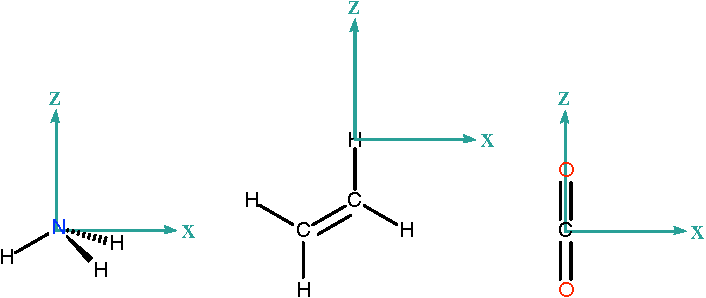
\includegraphics[width=0.9\textwidth]{anisotropic/figures/local_coords-crop.pdf}  
          \caption{Local axis system, shown for select atoms in molecules.}
          \label{fig:local_axis}
          \end{figure}

We next make an ansatz that \cref{eq:general_anisotropic_repulsion} is
separable into radial- and angular-dependent contributions,
%
\begin{align}
\label{eq:separable_anisotropic_repulsion}
%\erep_{ij}(r_{ij},\theta_i,\phi_i,\theta_j,\phi_j) \approx f(r_{ij})g(\theta_i,\phi_i,\theta_j,\phi_j),
\erep_{ij}(r_{ij},\theta_i,\phi_i,\theta_j,\phi_j) \approx 
\vrep_{ij}(r_{ij},\theta_i,\phi_i,\theta_j,\phi_j) = \fij \gij
\end{align}
%
thus subdividing the problem of finding a general functional form for $\erep_{ij}$ into
two more tractable tasks. First, we must find an ideal sum-of-spheres model to
describe the radial (isotropic) dependence of the force field, and second, we must find
a way to model the orientation dependence as a multiplicative
pre-factor to \fij.

% TODO: Include a discussion of additional forms for \fij that might serve as
% good functional forms upon which gij can be added?
Given that the only requirement for \fij is that it be isotropic, how should a
suitable model for \fij be chosen?
Indeed, all standard isotropic force fields are of this general form, and thus
might serve as a suitable starting point for anisotropic force field development.
For reasons discussed below, in this Chapter we employ 
a simple and accurate model (\isaffold) from \cref{ch:isaff} for \fij. This
model can be
derived from first-principles by approximating $\erep_{ij}$ as proportional to
the overlap %, $S_{\rho}^{ij}$,
between spherically-symmetric atom-in-molecule (AIM) electron densities, each with density
\begin{align}
\rho_i(r) = D_i \exp^{-B_i r},
\end{align}
where $D_i$ and $B_i$ are both atom type-specific constants that can be parameterized from
molecular electron densities and that represent, respectively,
the shape and hardness of the AIM density. Using this approximation to the
overlap model,
\cite{Kim1981,Nyeland1986,Ihm1990,Stone2007,Wheatley1990,Mitchell2000,Soderhjelm2006,Day2003}
the exchange energy between two atoms is then modeled by
%
\begin{align}
\begin{split}
\label{eq:fij}
\erep_{ij} \approx \vrep_{ij} &\propto S_{\rho}^{ij} \\
&\approx \Aex{ij} \left( \frac{ (\B\R)^2}{3} + \B\R + 1 \right) \exp(-\B\R) 
\end{split}
\intertext{with combining rules} 
\begin{split}
\label{eq:aij}
\Aex{ij} 
&\equiv \Aex{i}\Aex{j},\\
\B &\equiv \sqrt{B_iB_j}. \\
\end{split}
%
\end{align}
%
$S_{\rho}^{ij}$ is the electron density overlap between atoms and \A is
a fitted proportionality constant.

Here and throughout we use \cref{eq:fij}
as our
model for \fij. This choice is primarily justified in \cref{ch:isaff} by the
previously-demonstrated accuracy of the Slater-ISA formalism as compared to other
sum-of-spheres models for repulsion.\cite{VanVleet2016} 
Furthermore, and especially for simple test cases where one
might expect the sum-of-spheres approximation to hold (such as with argon, methane, or ethane), we have shown (see
\cref{ch:isaff}) that the \isaffold
correctly models intermolecular potential energy surfaces for a sizable library of intermolecular
interactions over the asymptotic, attractive, and repulsive regions of
the PES.

In addition to this empirical motivation for using the Slater-ISA formalism,
there are good theoretical grounds to utilize it as a model for \fij.
Specifically, the AIM densities used to parameterize \isaffold are
partitioned using an iterated stockholder atoms (ISA) procedure,
and the resulting density profiles are guaranteed to be maximally spherical.
\cite{Misquitta2014,Lillestolen2008,Lillestolen2009}
%DISCUSS: Alston, to what extent is this true? That is, are the BS-ISA
%densities algorithmically guaranteed to converge to maximally-spherical
%shapes, or does this just empirically seem to be true in practice?
This condition of `maximum sphericity' has two consequences. First, it
suggests that the resulting \isaffold should be an optimal, or nearly optimal,
isotropic atom-atom model. In other words, there is good reason to hope that
our model for \fij completely accounts for
the radial dependence of the potential, and consequently that models for \gij
will truly represent the orientation dependence rather than simply over-fitting
residual errors from the radial functional form, thus retaining high
transferability. 
Second, and relatedly,  having
maximally-spherical ISA densities suggests that anisotropic effects should be a
minimal perturbation to the PES. This means that, to a first-order
approximation, \gij is simply equal to 1. Furthermore, the non-spherical
components of the ISA densities should provide us
with guidance as to which atom types might require anisotropic treatment.

With the functional form for \fij determined, we now describe our
model for \gij. As motivated in \appendixref{sec:appendix}, and under
the ansatz of radial and angular separability,
an approximate, transferable, and orientation-dependent expression for \Aex{i} can be obtained
by expanding \Aex{i} in a
basis of 
renormalized spherical harmonics,
\begin{align}
\label{eq:sph_harm}
C_{lm}(\theta,\phi) = \sqrt{\frac{4\pi}{2l+1}}Y_{lm}(\theta,\phi).
\end{align}
thus yielding
%
\begin{align}
\label{eq:gij}
\begin{split}
\Aex{i}(\theta_i,\phi_i) &= 
\Aex{i,\text{iso}}\big(1 + \aniso{exch} \big), \\
\aniso{exch} &\equiv \sum\limits_{l>0,k} \aex  C_{lk}(\theta_i,\phi_i)
\end{split}
\end{align}
%
for \Aex{i} and subsequently
%
\begin{align}
\label{eq:vex}
\vrep_{ij} &= \Aex{ij}(\Omega_{ij})
        \left( \frac{ (\B\R)^2}{3} + \B\R + 1 \right) \exp(-\B\R)
\end{align}
with
\begin{align}
\Aex{ij}(\Omega_{ij}) &= \Aex{i}(\theta_i,\phi_i)\Aex{j}(\theta_j,\phi_j)
\end{align}
%
for the exchange-repulsion potential. Note that, with the exception of the
now orientation-dependent \Aex{i}, the atomically-anisotropic model in \cref{eq:vex} is identical to
our previously-defined isotropic model (\cref{eq:fij}). 

In terms of parameterization for our newly-developed anisotropic model, note
that the \aex are free parameters which must be fit to ab initio
data. 
Still, we and others have found the expansion in \cref{eq:gij} to be very quickly convergent,
\cite{Stone2007,Mitchell2001,Price2000,Stone1988,Day2003,Torheyden2006,Totton2010,Misquitta2016,Price2010a}
 especially given a proper choice of coordinate
system that eliminates many expansion terms via symmetry. In practice, only
symmetry-allowed terms up
to $l=2$ seem to be required for heteroatoms, carbons in multiple bonding
environments, and select hydrogens (see
equations in \cref{sec:results}), while many other atom types require no anisotropic
parameters whatsoever. Encouragingly,
isotropic atom types are easily modeled within
this formalism simply by setting $\aniso{} = 0$.

\end{subsubsection}
\begin{subsubsection}{Other Short-Range Effects}

As in \cref{ch:isaff},\cite{VanVleet2016} we have found that other short-range effects, namely charge
penetration and short-range induction, can be modeled as proportional to
exchange-repulsion. We take the same approach in the present Chapter, and
the functional form for these two short-range effects is given by
\cref{eq:vex}, with `exch' superscripts replaced by the appropriate short-range
energy term (see \cref{sec:methods}).
Additionally, for induction, the long-range polarization must be damped, and
for now this damping is modeled isotropically
as in the AMOEBA force field.\cite{Shi2013} 
%
Finally, to model short-range dispersion, we
take the same Tang-Toennies\cite{Tang1984,Tang1992} damping approach as in
\cref{ch:isaff}.\cite{VanVleet2016} Because the argument to the damping function is given by 
\[
x = -\frac{d}{dr}\left[\ln \vrep(r)\right] \ r,
\]
and because anisotropy only enters into the functional form as a
multiplicative pre-factor, our functional form for damping remains unchanged
compared to our previously-derived isotropic model.\cite{VanVleet2016}

\end{subsubsection}
\end{subsection}

\begin{subsection}{Anisotropic Models for Long-Range Interactions}

\begin{subsubsection}{Electrostatics}

Theories for including anisotropy in long-range electrostatics are well
established, and we refer the reader
elsewhere for complete details on the required formalisms for distributed multipole approaches.
\cite{stone2013theory,Stone2007}
In the present Chapter, 
\[
V^{\text{multipole}}_{ij} = \vmultipole
\]
with multipolar interaction tensor $T$ and parameterized moments $Q$ for all
multipole moments $tu$ up to (in the present Chapter) rank 2.

On the grounds of increased accuracy and ease of parameterization, here we have chosen 
to use a multipolar approach to describe the anisotropy of
long-range electrostatics,
However, for increased computational efficiency, off-site point charge models
\cite{Cardamone2014}
could also be utilized.

\end{subsubsection}
\begin{subsubsection}{Induction}

Just as with electrostatics, long-range induction should properly be described
by a distributed multipole expansion of interacting atomic
polarizabilities.\cite{Stone2007,Misquitta2016} Indeed, it has been shown
that inclusion of higher-order and/or anisotropic polarizabilities greatly
reduces errors in the two-body induction potential relative to commonly-used isotropic
dipole polarizability models.\cite{Misquitta2008b,Holt2008,Holt2010,Schmidt2015,Shi2013}
Because the model for the two-body induction also determines the many-body
polarization energy, the proper treatment of induced multipoles becomes especially
important in condensed phase simulation.\cite{stone2013theory,Schmidt2015,Shi2013}

Owing to the increased computational cost of these higher-order and anisotropic polarizability
models, and because such functional forms are (as of now, and to our
knowledge) not fully implemented in common molecular simulation packages, we
neglect
both higher-order and anisotropic contributions to the long-range induction in
the present Chapter. As
we shall show, however, errors in the induction potential limit the overall accuracy of
our force fields for extremely polar molecules (notably water), and
further improvements will likely require us to generate improved models for long-range induction. 

\end{subsubsection}
\begin{subsubsection}{Dispersion}

Past research\cite{stone2013theory} has motivated an anisotropic atom-atom model for dispersion 
of the form
%
% TODO: Check the limits on this equation
\begin{align}
\label{eq:stone_disp}
\vdisp_{ij} = - \sum\limits_{n=6} \frac{C_{ij,n}(\Omega_{ij})}{\R^n}
\end{align}
%
Note that, in this equation, both odd and even powers of $n$ are allowed in the
dispersion expansion.
In order to make this model both computationally efficient and maximally compatible with our previous isotropic
model for dispersion, 
%% and in a manner analogous to our treatment of
%% short-range overlap effects, 
we choose (as an ansatz) to model the dispersion anisotropy as an
orientation-dependent prefactor that effects all isotropic $C_6 - C_{12}$ dispersion
coefficients equally:
%
\begin{align}
\label{eq:mastiff_disp}
\vdisp_{ij} &= - \Adisp{i}\Adisp{j}\sum\limits_{n=3}^{6} \frac{C_{ij,2n}}{\R^{2n}} 
\intertext{with}
\label{eq:mastiff_disp2}
\Adisp{i} &= 1 + \aniso{disp}
\end{align}
%
and \aniso{disp} as in \cref{eq:gij}.
%% Because $C_{00}(\theta,\phi) = 1$, the anisotropy expansion proposed above has
%% no effect on the average magnitude of the various dispersion coefficients.
Once again, \cref{eq:mastiff_disp} reduces to the isotropic case by setting
$\aniso{disp} = 0$.
%
We must note that, though the functional form in \cref{eq:mastiff_disp} bears many similarities to
\cref{eq:stone_disp}, (unphysically) no odd powers of $r$ show
up in our proposed model for dispersion. Furthermore, 
the model utilizes the same anisotropic expansion for each dispersion
coefficient.
Nonetheless, we will show in \cref{sec:results}
that this model yields significant accuracy gains in the dispersion energy
with only minimal additional parameterization and model expense.

\end{subsubsection}


\end{subsection}


\end{section}
%%%%%%%%%%%%%%%%%%%%%%%%%%%%%%%%%%% Theory %%%%%%%%%%%%%%%%%%%%%%%%%%%%%%%%%%%%%%%%





%%%%%%%%%%%%%%%%%%%%%%%%%%%% Computational Details %%%%%%%%%%%%%%%%%%%%%%%%%%%%%%%%
\begin{section}{Technical Details}
\label{sec:methods}

\begin{subsection}{The 91 Dimer Test Set}

Our benchmarking procedures
are the same as in \cref{ch:isaff},\cite{VanVleet2016}
and we briefly summarize the relevant technical details. A full discussion of
results and example calculations are presented in \cref{sec:results}.

We have previously developed a large library of benchmark energies
for interactions between the following 13 atomic and organic species: acetone, argon, ammonia, carbon dioxide,
chloromethane, dimethyl ether, ethane, ethanol, ethene, methane, methanol,
methyl amine, and water. Using these 13 monomers, we have generated a library of dimer interaction
energies for each of the 91 possible unique dimer combinations (13 homomonomeric, 78
heteromonomeric). For each of these dimer combinations, interaction energies were
computed at a DFT-SAPT
\cite{Misquitta2002,Misquitta2003,Misquitta2005,Heßelmann2005a,Podeszwa2006a,Heßelmann2002,Heßelmann2003,Heßelmann2002a,Jansen2001}
level of theory for 1000 quasi-randomly chosen dimer configurations,
representing 91,000 benchmark interaction energies in total. 
As described below, parameters for a given force field methodology are then
fit on a component-by-component basis to reproduce the benchmark DFT-SAPT energies. 

\end{subsection}
\begin{subsection}{Parameter Determination}

We will present three types of force field fitting methodologies in this
Chapter,
termed \isoff, \isaff, and \anisoff (alternately referred to as \mastiff, as
discussed below). The nomenclature of each
name refers to, first, the isotropic/anisotropic treatment of multipolar
electrostatics and, second, the isotropic/anisotropic treatment of dispersion
and short-range effects. 
All studied force fields
use the following general functional form:
%
\begin{align}
%
\label{eq:ff_form}
\vtot &= \sum\limits_{ij} \vrep_{ij} + \velst_{ij} + \vind_{ij} + \vdhf_{ij} +
\vdisp_{ij} 
\intertext{where}
\begin{split}
\label{eq:ff_details}
\vrep_{ij} &= \Aex{ij} P(B_{ij}, r_{ij}) \exp(-B_{ij}r_{ij}) \\
\velst_{ij} &= -\Ael{ij} P(B_{ij}, r_{ij}) \exp(-B_{ij}r_{ij}) + \vmultipole
\\
\vind_{ij} &= -\Aind{ij} P(B_{ij}, r_{ij}) \exp(-B_{ij}r_{ij}) + \vdrudeind \\
\vdhf_{ij} &= -\Adhf{ij} P(B_{ij}, r_{ij}) \exp(-B_{ij}r_{ij}) +
\vdrudescf \\
\vdisp_{ij} &= - \Adisp{ij} \sum\limits_{n=3}^{6} f_{2n}(x) \frac{C_{ij,2n}}{r_{ij}^{2n}}
\\
P(B_{ij},r_{ij}) &= \frac13 (B_{ij} r_{ij})^2 + B_{ij} r_{ij} + 1 \\
\A &= A_iA_j \\
\B &= \sqrt{B_iB_j} \\
\C &= \sqrt{C_{i,2n}C_{j,2n}} \\
f_{2n}(x) &= 1 - e^{-x} \sum \limits_{k=0}^{2n} \frac{(x)^k}{k!} \\
x &= B_{ij}r_{ij} - \frac{2 B_{ij}^2 r_{ij} + 3 B_{ij} }
{ B_{ij}^2 r_{ij}^2 + 3 B_{ij} r_{ij} + 3} r_{ij}
\end{split}
\end{align}
%
For both \isoff and \isaff, $A_i$ is a fit parameter, and
$\Adisp{ij} = 1$. For \isoff (our completely isotropic model), the multipole expansion
\vmultipole is truncated to point charges, whereas \isaff and \mastiff both use a
multipole
expansion up to quadrupoles.
Finally, for
our anisotropic model, \mastiff, 
each $A_i$ is treated as an orientation-dependent function, and is represented
by the spherical harmonic
expansion 
\begin{align}
\label{eq:v_aniso}
\begin{split}
A_{i}(\theta_i,\phi_i) &= 
A_{i,\text{iso}}\big(1 + \aniso{} \big), \\
\aniso{} &\equiv \sum\limits_{l>0,k} a_{i,lk}  C_{lk}(\theta_i,\phi_i)
\end{split}
\end{align}
where $A_{i,\text{iso}}$ and $a_{i,lk}$ are fitted parameters with the
exception that $A_{i,\text{iso}}^{\text{disp}} = 1$.

%% %
%% \begin{align}
%% \label{eq:a_params}
%% A_{i}(\theta_i,\phi_i) = A_{i,\text{iso}}\left(1 + \sum\limits_{l>0k} a_{i,lk}
%% C_{lk}(\theta_i,\phi_i)\right)
%% \end{align}
%% %

Because DFT-SAPT provides a physically-meaningful energy decomposition into electrostatic,
exchange-repulsion, induction, and dispersion terms, parameters for each term in
\cref{eq:ff_form} are directly fit to model the corresponding DFT-SAPT energy
(see \citen{VanVleet2016} and references therein for details on the DFT-SAPT
terminology): 
%
\begin{align}
\begin{split}
\vrep \approx \erep &\equiv E^{(1)}_{\text{exch}} \\
\velst \approx \eelst &\equiv E^{(1)}_{\text{pol}} \\
\vind \approx \eind &\equiv E^{(2)}_{\text{ind}} + E^{(2)}_{\text{ind-exch}} \\
\vdhf \approx \edhf &\equiv \delta(\text{HF}) \\
\vdisp \approx \edisp &\equiv E^{(2)}_{\text{disp}} + E^{(2)}_{\text{disp-exch}}.
\end{split}
\end{align}
%
Fitting parameters on a component-by-component basis helps ensure parameter
transferability and minimizes reliance on error cancellation. Note that no
parameters are fit to reproduce the total energy and that,
because the DFT-SAPT energy decomposition is only calculated to second-order, 
third- and higher-order terms (mostly consisting of higher-order induction)
are estimated by \edhf.

\begin{subsubsection}{Parameters Calculated from Monomer Properties}

Of the parameters listed in \cref{eq:ff_details}, most do not need to be
fit to the DFT-SAPT energies, but can instead be calculated directly on the
basis of monomer electron densities. In particular, all multipolar
coefficients, $Q$, polarizabilities (involved in the calculation of \vdrude),
dispersion coefficients $C$, and atom-in-molecule exponents, $B^{\text{ISA}}$, are calculated in a manner nearly
identical to \citen{VanVleet2016}. Note that, for our atom-in-molecule exponents, we tested
the effects of treating $B^{\text{ISA}}$ both as a hard- and as a
soft-constraint in the final force field fit. While the conclusions from this
study are rather insensitive to this choice of constraint methodology, we have
found that the overall force field quality is somewhat improved by
relaxing the $B^{\text{ISA}}$ coefficients in the presence of a harmonic
penalty function (technical details of which can be
found in the Supporting Information of \citen{VanVleet2016}). The optimized $B$
coefficients in this Chapter are always within 5--10\% of the calculated $B^{\text{ISA}}$
coefficients from \cref{ch:isaff}, demonstrating the good accuracy of the $B^{\text{ISA}}$
calculations themselves.

As a second distinction from our prior work, and for reasons of compatibility
with the OpenMM\cite{Eastman2013} software we use for all molecular dynamics
simulations, here our molecular simulations use an induced
dipole model to describe polarization effects.
Numerical differences between this
model and the drude model used previously are very minor.
Additionally, the Thole-damping functions used in this Chapter follow
the same functional form used in the AMOEBA model,\cite{Ren2003} with a damping
parameter of 0.39. 

\end{subsubsection}
\begin{subsubsection}{Parameters Fit to Dimer Properties}

In addition to the soft-constrained $B$ parameters, all other free parameters
($A$ and $a$ parameters from \cref{eq:ff_form}
and \cref{eq:v_aniso}) are fit to reproduce
DFT-SAPT energies from the 91 dimer test set described above. For each dimer
pair, 4-5 separate optimizations (for exchange, electrostatics, induction,
\dhf, and, for \mastiff, dispersion) were carried out to minimize a weighted
least-squares error, with the weighting function given by a Fermi-Dirac functional
form,
%
\begin{align}
\label{eq:weighting-function}
w_i = \frac{1}{\exp(-E_i/kT) + 1},
\end{align}
%
where $E_i$ is the reference energy and 
the parameter $kT$, which sets the energy scale for the
weighting function, is calculated from an estimate of the global minimum well
depth, 
$E_{\text{min}}$, such that
$kT = 5.0 |E_{\text{min}}|$. 

\end{subsubsection}
\begin{subsubsection}{Local Axis Determination}

Identically to AMOEBA and other force fields that incorporate some degree of
atomic-level anisotropy,\cite{Ren2003,Day2003,Totton2010} we use a z-then-x
convention to describe the relative orientation of atomic species. By design,
the z-axis is chosen to lie parallel to the principal symmetry axis (or
approximate local symmetry axis) of an atom
in its molecular environment, and the xz-plane is similarly chosen to
correspond to a secondary symmetry axis or plane. Based on the assigned symmetry
of the local reference frame, many terms in the
spherical expansion of \cref{eq:gij} can then be set to zero, minimizing the
number of free parameters that need to be fit to a given atom type. 
%TODO: Add to SI
Representative local reference frames are shown for a few atom types in
\cref{fig:local_axis}, and a complete listing of anisotropic atom types
(along with their respective local reference frames and non-zero spherical
harmonic expansion terms)
are given in the \cref{sec:mastiff-local_axis_defs}.

\end{subsubsection}
\begin{subsubsection}{CCSD(T) Force Fields}

DFT-SAPT is known to systematically underestimate the interaction energies of
hydrogen-bonding compounds, and can also exhibit small but important errors
for dispersion-dominated compounds.\cite{Parker2014} Consequently, for
simulations involving \co, \cl, \nh, and \ho, we refit our SAPT-based force
fields to reproduce benchmark supermolecular, counterpoise-corrected CCSD(T)-F12a/aVTZ
calculations on the respective dimers. All calculations were performed using
the Molpro 2012 software.\cite{MOLPRO} Fits were still performed on a
component-by-component basis, with the energy of most components matching the
DFT-SAPT calculations used in \cref{ch:isaff}.\cite{VanVleet2016} However, so that
the total benchmark energy corresponded to the total interaction energy
calculated by CCSD(T)-F12a/aVTZ, the difference between coupled-cluster and
SAPT energies was added to the SAPT dispersion energy,
%
\begin{align}
\begin{split}
\vrep \approx \erep &\equiv E^{(1)}_{\text{exch}} \\
\velst \approx \eelst &\equiv E^{(1)}_{\text{pol}} \\
\vind \approx \eind &\equiv E^{(2)}_{\text{ind}} + E^{(2)}_{\text{ind-exch}} \\
\vdhf \approx \edhf &\equiv \delta(\text{HF}) \\
\vdisp \approx \edisp &\equiv E^{(2)}_{\text{disp}} +
E^{(2)}_{\text{disp-exch}} + \delta(\text{CC}),
\end{split}
\end{align}
%
where $\delta(\text{CC}) \equiv E_{\text{int}}^{\text{CCSD(T)-F12a}} -
E_{\text{int}}^{\text{DFT-SAPT\phantom{()}}}$.
%

In fitting these CCSD(T)-f12a-based force fields, and to account for small
errors in the original SAPT dispersion energy, we somewhat relaxed the
constraint that $\Adisp{} = 1$ for all atom types, and instead let $ 0.7 \le
\Adisp{} \le 1.3$. This constraint relaxation led, in some cases, to modest
improvements in the fitted potential.


\end{subsubsection}

\begin{subsubsection}{\co 3-body potential}
For the \co dimer, we developed a three-body model to
account for three-body dispersion effects. This three-body model is based on
the three-body dispersion Axilrod-Teller-Muto (ATM) type model developed by \citeboth{Oakley2009a}. These
authors fit the ATM term with the constraint that the total molecular $C_9$
coefficient be 1970 a.u. Based on our own calculations using a CCSD/AVTZ
level of theory,\cite{Korona2011} we have obtained an
isotropic molecular $C_9$ coefficient of 2246 a.u.; consequently, a 1.13 universal
scale factor was introduced to the Oakley potential so as to obtain dispersion
energies in line with this new dispersion coefficient.
\end{subsubsection}

\end{subsection}

%% \begin{subsection}{Comparison to Ab Initio Benchmarks}
%% 
%% As in previous work, root-mean-square (\rmse) and mean-signed errors (MSE),
%% both with respect to the DFT-SAPT reference energies,
%% were calculated for each methodology and for each dimer pair. Similarly,
%% `attractive \rmse/MSE' (a\rmse/aMSE) were computed by only considering the
%% subset of dimer configurations with net attractive total energies (as measured
%% by DFT-SAPT). After taking the absolute value of the MSE values, the
%% various error metrics were then averaged in the geometric mean sense to
%% obtain one `characteristic' \rmse or \mse for the entire 91 dimer
%% test set.
%% 
%% \end{subsection}
\begin{subsection}{Simulation Protocols}



\begin{subsubsection}{\deltahsub for \co}

For \co, the molar enthalphy of sublimation was determined according to 
%
\begin{align}
\begin{split}
\deltahsub &= H_{\text{g}} - H_{\text{crys}}  \\
           &= (U_{\text g} + PV_{\text g}) - (U_{\text{el,crystal,0K}} 
                +\Delta U_{\text{el,crystal,0K}\to T_{\text{sub}}} + PV_{\text{crys}} + E_{\text{vib,crystal}}) \\
           &\approx (RT) - \left(U_{\text{el,crystal,0K}} 
                + \int_{0K}^{T_\text{sub}} C_p dT \quad + E_{\text{vib,crystal}}\right) \\
\end{split}
\end{align}
%
which assumes ideal gas behavior and $PV_{\text{g}} >> PV_{\text{crys}}$.
For the crystal, an experimental measure of $C_p$ was obtained from \citen{Giauque1937} and numerically
integrated to obtain a value $\Delta U_{\text{el,crystal,0K}\to
T_{\text{sub}}} = 6.70 \kjmolold$. Theoretical measures of
$E_{\text{vib,crystal}} \approx 2.24 - 2.6 \kjmolold$ were obtained from
(respectively) \citen{Cervinka2017} and \citen{Heit2016a}, 
and
$U_{\text{el,crystal,0K}}$ was determined from the intermolecular force field
using a unit cell geometry taken from experiment.\cite{Simon1980}

\end{subsubsection}
\begin{subsubsection}{Other \co Simulations}

To determine the densities and enthalpies of vaporization used in this Chapter,
simulations were run in OpenMM using NPT and NVT ensembles, respectively. After an
equilibration period of at least 100ps, data was collected for a minimum of 500ps, and
uncertainties were calculated using the block averaging method. Average densities
were obtained directly from simulation, and 
the molar enthalpy of vaporization for \co was determined from the following
formula:
%
\begin{align}
\begin{split}
\deltahvap &= H_{\text{g}} - H_{\text{liq}} \\
           &= U_{\text{g}} - U_{\text{liq}} + P(V_{\text{g}} - V_{\text{liq}})
\end{split}
\end{align}
%
Note that, at the state points studied, the ideal gas approximation is
insufficiently accurate, and thus simulations were run for both the gas and
liquid phases at experimentally-determined
densities and pressures.\cite{Span1996}

\end{subsubsection}
\begin{subsubsection}{2\textsuperscript{nd} Virial Calculations}

Classical second virial coefficients were calculated for \nh, \ho, \co,
and \cl using rigid monomer geometries and following the procedure described in
\citen{McDaniel2013}.


\end{subsubsection}
\end{subsection}




\end{section}
%%%%%%%%%%%%%%%%%%%%%%%%%%%% Computational Details %%%%%%%%%%%%%%%%%%%%%%%%%%%%%%%%




%%%%%%%%%%%%%%%%%%%%%%%%%%%%%%%%%% Results %%%%%%%%%%%%%%%%%%%%%%%%%%%%%%%%%%%%%%%%
\begin{section}{Results and Discussion}
\label{sec:results}


\begin{subsection}{Overview}

We now turn to a discussion of the methods whereby we can compare our newly
developed anisotropic force field methodology to various
sum-of-spheres models. 
As is standard in ab initio force field development, we use a
straightforward metric to evaluate force field quality:
the accuracy with which a given force field functional form can reproduce
high-quality ab initio benchmark energies. Furthermore, and because the
functional forms introduced in \cref{sec:theory} directly affect only the
pairwise-additive portion of the intermolecular potential, we
concentrate our efforts on assessing force field with respect to benchmark
calculations of dimer interaction energies, which directly measure the
two-body portion of a system's total intermolecular interaction energy.
(When required, and as discussed in \cref{sec:co2}, many-body effects can be accounted for separately
and systematically using known methods).\cite{Yu2012b,McDaniel2014}
%
In addition to this primary metric for force field quality, we also evaluate our force
fields for their ability to reproduce select experimental properties.
Importantly, however, 
experimental predictions from an ab initio force field significantly depend, not only on the
fit quality of the pair potential, but also on the 
choice of benchmark electronic structure theory, treatment of many-body and/or quantum
effects, etc. 
Because these factors complicate comparisons to experiment, here
we treat experimental accuracy as an important, but secondary, metric for evaluating force
field accuracy. 

So as to systematically evaluate the effects of anisotropy on the development of
intermolecular potentials, we compare three types of models.
The first model, which we call \isoff, uses a completely isotropic description
of all energy components. Our second model, \isaff, accounts for long-range electrostatic
anisotropy by including multipolar contributions (up to
quadrupoles), but uses an isotropic model for all other terms in the
intermolecular force field.
Note that this model is virtually identical to the \isaffold
model developed in \cref{ch:isaff}, and that this manner of partially
treating anisotropy is very similar in spirit to the popular AMOEBA\cite{Ren2003,Shi2013}
methodology. Finally, we develop \anisoff, which selectively incorporates anisotropy into all
energy components (aside from long-range polarization) of the intermolecular potential.
This model, which we also refer to with the moniker \mastiff (a
\textbf{M}ultipolar, \textbf{A}nisotropic, \textbf{S}later-\textbf{T}ype
\textbf{I}ntermolecular \textbf{F}orce \textbf{F}ield), treats all
electrostatic interactions via a multipole expansion with up to quadrupolar
contributions, and includes anisotropic parameters for other terms of the force field
(short-range interactions plus dispersion) for heteroatoms, atoms in
multiple bonding environments, and associated hydrogens. A complete list of anisotropic atom types is
given in the \cref{sec:mastiff-local_axis_defs}.

\end{subsection}
\begin{subsection}{Accuracy: Comparison with DFT-SAPT}

For each of the 91 dimer combinations described in \cref{sec:methods},
parameters were fit to reproduce \sapt energies calculated for 1000 different
relative orientations of the constituent monomers. 
From these `dimer-specific' fits, and as in
described in \cref{ch:isaff},\cite{VanVleet2016} we then averaged the
root-mean-squared (\rmse) and mean signed errors (\mse) from each of the 91
fits to produce so-called `characteristic \rmse/\mse', metrics
representative of the errors associated with a given force field methodology.
Typically, because the absolute magnitudes of the various energy components
become large in the repulsive portion of the potential, these characteristic
errors are dominated by repulsive
configurations. As such,
we have also calculated `attractive
\rmse/\mse' (a\rmse/a\mse), defined as the characteristic errors for the subset
of configurations with net attractive total interaction energies. 
All computed characteristic \rmse are shown in \cref{fig:rmse}.
Unless otherwise stated, results in this section refer
exclusively to the `Dimer-specific' fits in \cref{fig:rmse}, with an
explanation and full discussion of so-called `Transferable' fits given in
\cref{sec:transferability}.

    %%%%%%%%%%%% Average RMSE %%%%%%%%%%%%%%%
    \begin{figure}
    \centering
    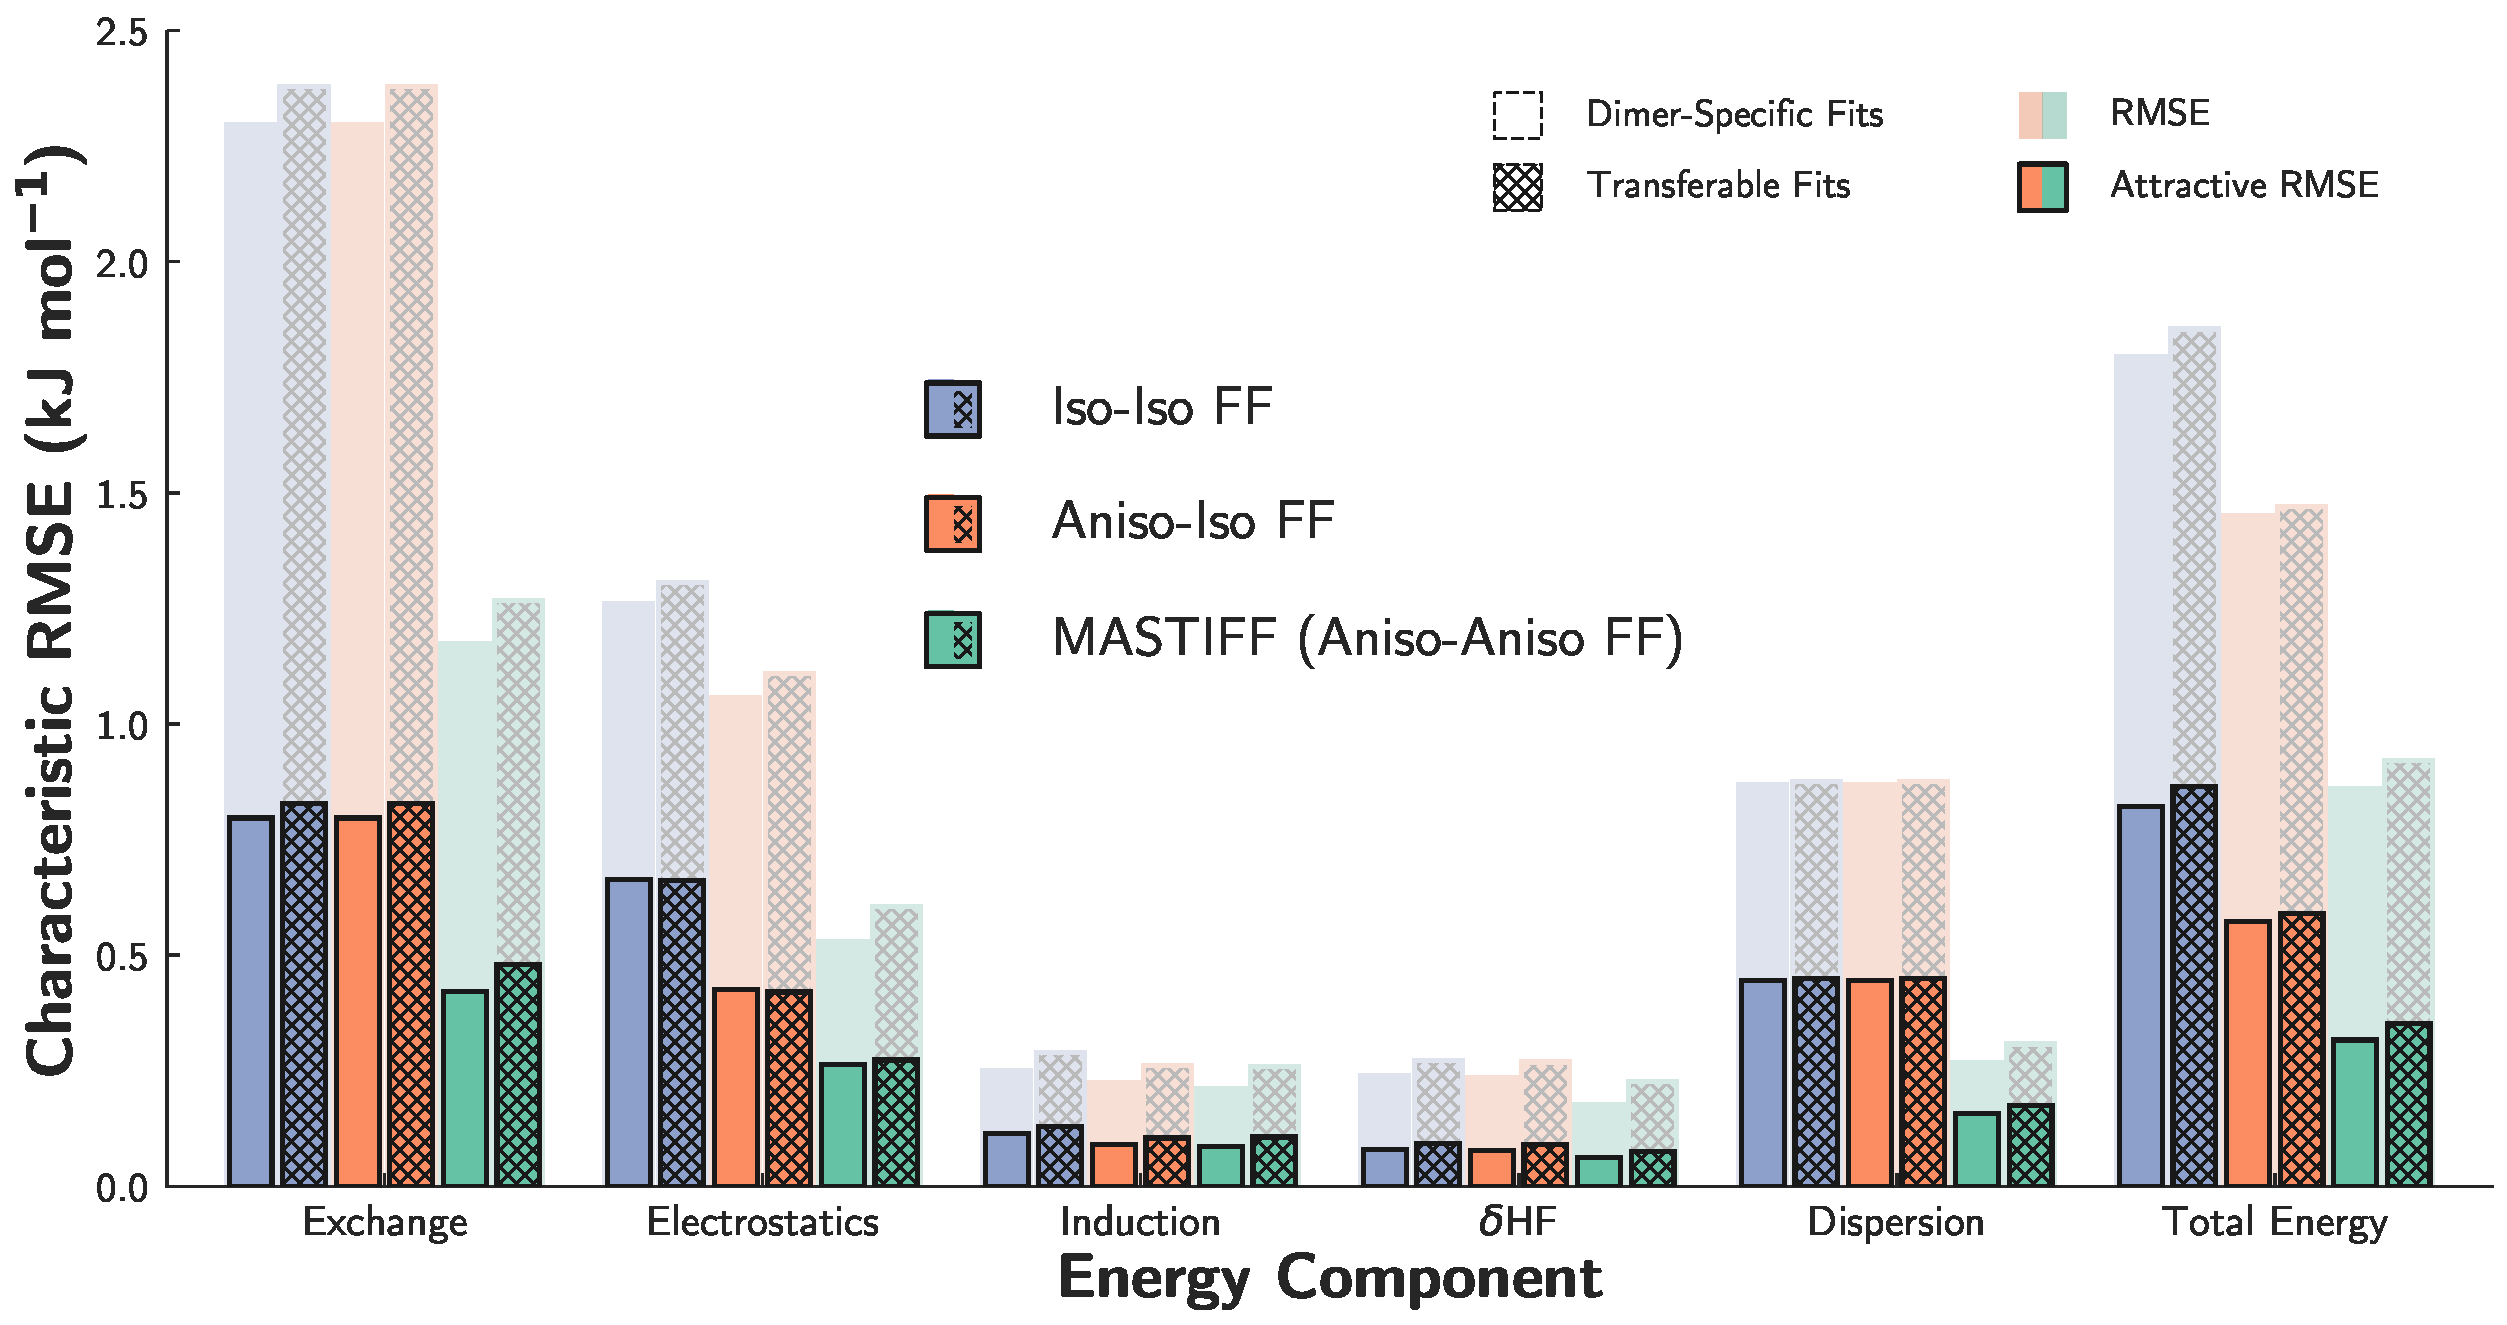
\includegraphics[width=0.9\textwidth]{anisotropic/rmse_comparisons/transferability_rmse_errors.pdf}
    \caption{
    Characteristic RMSE (as described in the main text) for the \isoff
(purple), \isaff (orange), and \mastiff (green) over the 91
    dimer test set. The semi-transparent bars represent total RMSE
    for each energy component, while the smaller solid bars represent `Attractive'
    RMSE, in which repulsive points have been excluded. For each force field,
    two types of fits, dimer-specific (solid) and transferable (hashed lines),
    are displayed; see \cref{sec:transferability} for details. Finally, note that, for \isoff and \isaff, only the electrostatic
    and total energy \rmse's differ. 
            }
    \label{fig:rmse}
    \end{figure}
    %%%%%%%%%%%% Average RMSE %%%%%%%%%%%%%%%

Based on the characteristic \rmse shown in \cref{fig:rmse}, both \isaff
and \mastiff offer substantial improvements over the completely isotropic model
\isoff. Though unsurprising, given the well-studied importance of higher-order
electrostatic multipole moments, \isaff shows reduced \rmse/a\rmse that are (depending on the exact
error metric used)
roughly 30\% smaller than \isoff. 
Both \rmse and a\rmse measures showing similar gains in accuracy,
indicating that inclusion of higher-order multipoles (henceforth
`multipolar electrostatic anisotropy') is important in both
attractive and repulsive regions of the potential. Crucially, inclusion of
additional `short-range anisotropies' (anisotropic
interactions arising from overlap of monomer electron densities, namely
exchange-repulsion and electrostatic/inductive charge penetration) and
long-range `dispersion anisotropy' yields a \emph{further} 40\% reduction in
\rmse/a\rmse for \mastiff as compared to the \isaff.
This latter
result is highly important, as it suggests that, for the generation of highly
accurate ab initio potentials, the combination of short-range
and dispersion anisotropies 
are just as important to include as
multipolar electrostatic anisotropy. Indeed, this substantial increase in
force field accuracy, which arises from a full treatment of anisotropic
effects, and is independent of improvements from multipolar electrostatic anisotropy, 
is one of the most important findings in the present Chapter.
In summary, and encouragingly, the combination of multipolar electrostatic, short-range, and
dispersion anisotropies result in an overall 60\% reduction in \rmse/a\rmse when
comparing \isoff to \mastiff. 

To see exactly how an inclusion of anisotropy impacts each component of the
potential, \cref{fig:rmse} also displays characteristic \rmse/a\rmse for each term
in the force field description as compared to DFT-SAPT. Immediately, one can
see that (aside from induction, discussed below),
an inclusion of atomic-level anisotropy greatly improves the description of
each energy component. Unless otherwise stated, here we report results
for a\rmse and
dimer-specific fits, though similar values are obtained for overall \rmse and
for transferable fits.
Compared to \isoff, exchange errors in \mastiff
are reduced by 47\%. Electrostatic errors are reduced by an even larger
60\%. By evaluating the ratio of electrostatic errors between different
models, we find that $\sfrac{\text{a\rmse \isaff}}{\text{a\rmse \isoff}} = 0.64$
and $\sfrac{\text{a\rmse \mastiff}}{\text{a\rmse \isaff}} = 0.62$, suggesting
that \emph{both} higher-order multipoles and anisotropic charge penetration
terms are necessarily to obtain an accurate description of the DFT-SAPT
electrostatic energy. Finally, via an inclusion of dispersion anisotropy,
a\rmse for dispersion are reduced by a significant
65\%. 
%% Especially for dispersion, some of this error reduction may simply be due to
%% the increased number of free parameters associated with anisotropic atom types.
%% (For dispersion, no free parameters are fit for isotropic atom types, while up
%% to three parameters are fit for anisotropic atom types. For 
%% functional forms describing penetration, by contrast, one free parameter is
%% fit for isotropic atom types, while up to four free parameters are fit for
%% anisotropic interactions). If we relax the constraint from
%% \cref{eq:ff_details} that $\Adisp{} = 1$, thus fitting at least one free
%% parameter per isotropic atom type, we find a somewhat smaller improvement factor for
%% dispersion a\rmse of 47\%, which is more similar to what was observed for the
%% exchange energy. Regardless, it is qualitatively clear that dispersion
%% anisotropy plays an imporant role in determining overall force field accuracy.

Though the trends for exchange, electrostatics, and dispersion universally
suggest the importance of including atomic-level anisotropy, trends for terms
describing the physics of polarization and charge-transfer (represented in
DFT-SAPT by induction and
\dhf) are less encouraging. On the one hand, including higher-order multipoles
substantially lowers \rmse for induction, with $\sfrac{\text{\rmse \isaff}}{\text{\rmse \isoff}} = 0.70$. 
Because both \isoff and \isaff use isotropic polarizabilities, and because the
induction energy fundamentally depends only on the polarizabilities and the
static electric field, this
result is clearly due to an improved treatment of the static electric field
via anisotropy of the multipolar electrostatics.
Once again, this
suggests that an 
anisotropic treatment of long-range electrostatics is crucial for accurate
force field development. On the other hand, our functional form for anisotropic short-range
induction (\cref{eq:ff_form} and \cref{eq:v_aniso}) leads to no improvement in the
induction \rmse, with $\sfrac{\text{\rmse \isaff}}{\text{\rmse \isoff}} =
0.97$. This observed lack of improvement is likely due to a combination of
factors. First, and perhaps most importantly,
we have chosen in this Chapter to use isotropically-averaged dipole
polarizabilities, but as with
electrostatics, anisotropy and higher-order terms have been shown to be important in in the multipole
expansion of atomic dipole polarizabilities. 
\cite{Stone2007,Misquitta2007a,Misquitta2008b,Misquitta2016,Harder2006}
Second, and though probably a smaller source of error,
it is also unclear how to optimally
model the distance dependence of the induction energy at short
intermolecular separations, where penetration and charge-transfer effects
become important and the long-range polarization terms must be damped. 
\cite{VanVleet2016,Liu2017,Misquitta2013,Thole1981} 
Given that the more elaborate short-range form of the 
\mastiff induction model does not result in a tangible improvement, it is quite possible
that alternative formulations are required for an accurate treatment of highly
anisotropic induction.

    %% %%%%%%%%%%%% H2O Comparison %%%%%%%%%%%%%
    %% \begin{figure}[ht]
    %% 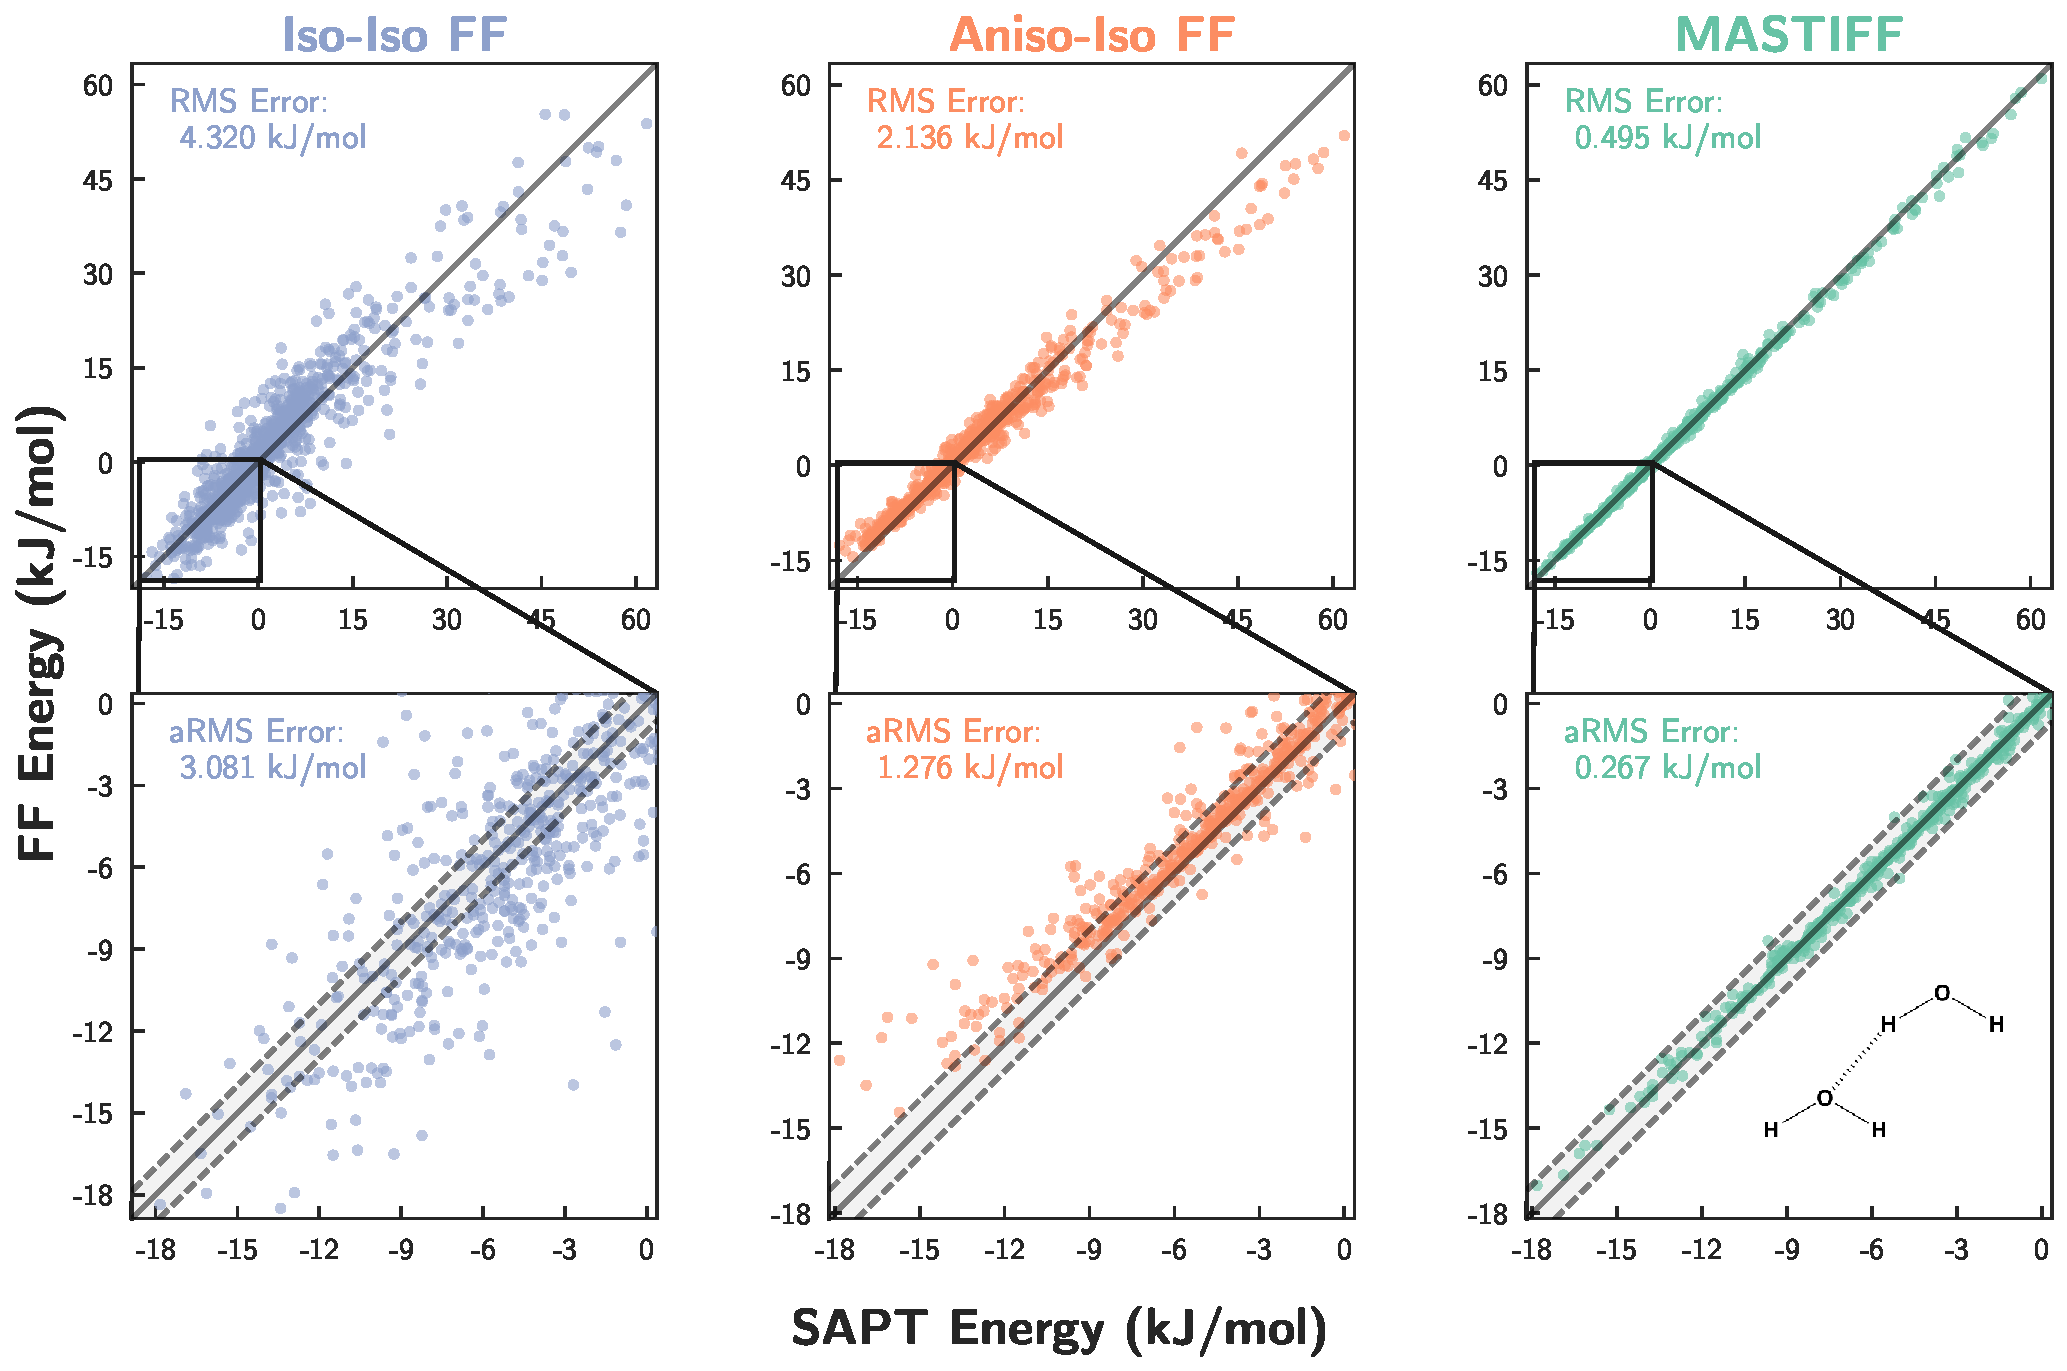
\includegraphics[width=0.9\textwidth]{figures/h2o_h2o_comparison.pdf}
    %% \caption{
    %%     Force field fits for the water dimer using \isoff (purple), \isaff (orange,
    %%     and \mastiff (green).
    %%     Fits for the total energy are displayed along
    %%     with an inset of the attractive regions. The solid $y=x$ line 
    %%     indicates perfect agreement between reference energies and each force field,
    %%     while dotted lines represent $\pm1$ \kjmolold error bounds. \rmse and a\rmse as in
    %%     the main text.
    %%         }
    %% \label{fig:h2o}
    %% \end{figure}
    %% %%%%%%%%%%%% H2O Comparison %%%%%%%%%%%%%

To further analyze the effects of anisotropy on a molecule-by-molecule basis, we have calculated
`improvement ratios', defined as 
$\sfrac{\text{a\rmse \isoff}}{\text{a\rmse \mastiff}}$,
for each energy component and for
each homomonomeric species in the test set, results for which are shown in
\cref{tab:ratios}. 
(Improvement ratios for heteromnomeric species are given in the \si of
\citen{VanVleet2017}, and we additionally provide
scatter plots of each homomonomeric force field fit in \cref{sec:mastiff-fits}.)

The most striking observation from the data presented in \cref{tab:ratios} is that
the improvement ratios vary considerably with molecule. For example, with water
the a\rmse is improved by an order of magnitude when anisotropy is included. On
the other hand, no improvement is seen for hydrocarbons such as ethane and
methane (also see the \cref{sec:mastiff-fits}). Consequently, anisotropy in the short-range expansions
may be necessary for only some atoms types (see \cref{sec:conclusions}). For the molecules
studied in our test set, and in line with chemical intuition, we have found
anisotropy to be particularly important for 
heteroatoms, $\pi$-bonded atoms,
and all hydrogens bonded to anisotropic heavy atoms. 
Appealingly, this distinction between anisotropic and
isotropic atom types 
simplifies force field parameterization and can enable more efficient molecular
simulation (via a more cost-effective treatment of multipolar electrostatics) without sacrificing force field accuracy.
Note that the current empirically-determined
definitions of anisotropic atom types
match both chemical intuition and the more quantitative measures
of atomic anisotropy proposed by other groups.\cite{Kramer2014,Wheatley2012}


    %%%%%%%%%%%% Error Ratios %%%%%%%%%%%%%%%
    \begin{table}[ht]
    \centering
    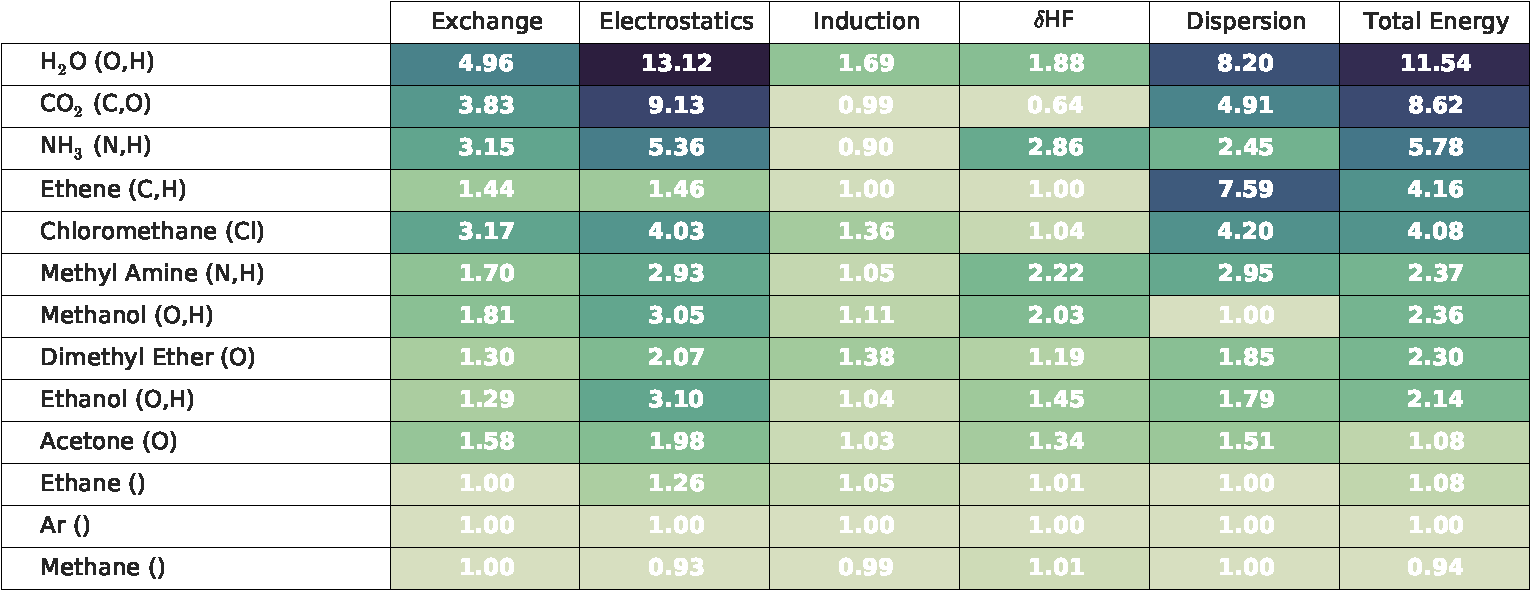
\includegraphics[width=0.9\textwidth]{anisotropic/figures/homodimer_error_ratios.pdf}
    \caption{
`Improvement Ratios' for each homomonomeric species in the
91 dimer test set. For each dimer and energy component, the improvement ratio
is calculated as the ratio of a\rmse between \isoff and \mastiff; values
greater than 1 indicate decreased errors in the anisotropic model. Entries have
been ordered according to the improvement ratio for the total energy.
            }
    \label{tab:ratios}
    \end{table}
    %%%%%%%%%%%% Error Ratios %%%%%%%%%%%%%%%


In general, the ordering of improvement ratios for exchange,
electrostatics, dispersion, and the total energies are reasonably correlated. (As stated above, our model
for anisotropic induction interactions is rather poor, and hence the
improvement ratios for induction and \dhf are relatively uncorrelated with the
other components. A good model for anisotropic induction and
\dhf might easily change this result). Physically speaking, all atomically-anisotropic
interactions arise from the same source (atomically-anisotropic
electron densities), and so the observed correlation might have been expected.
Nevertheless, there are some exceptions to this trend, such as with ethene and
acetone.
For ethene, relatively modest improvement ratios (roughly 1.4) are seen for exchange and
electrostatics, whereas dispersion shows a much greater improvement ratio of
7.6. Since ethene homomonomeric interactions are dispersion-dominated, the
improvement ratio for the total energy then roughly corresponds to that of dispersion.
A larger test set (particularly one which includes more non-polar
aromatic species) would be necessary to assess the generality of this result.
For acetone, there is good correlation between the improvement ratios for
exchange, electrostatics, and dispersion, which might lead one to suspect that
the total energy improvement ratio would also be around 1.5-2.0. Nevertheless, for this molecule, the
isotropic model benefits from error cancellation between energy components,
and the total energy a\rmse between isotropic and anisotropic models are
rather similar. 

Crucially, 
electrostatics is most definitely not the only intermolecular interaction for which
atomic-level anisotropy improves model quality. Indeed, for molecules like ethene, multipolar
anisotropy in the electrostatic model is relatively unimportant, whereas dispersion anisotropy is
essential for accurately modeling the $\pi$ interactions.
Thus, for a given system, multipolar electrostatic, dispersion, and/or short-range
anisotropies may all be important, and all relevant 
anisotropies must be accounted for in order to obtain good intermolecular
models.

\end{subsection}
\begin{subsection}{Transferability: Comparison to DFT-SAPT}
\label{sec:transferability}

From the above results it is clear that, when explicitly parameterized, an
inclusion of anisotropy can greatly enhance the accuracy of an intermolecular
potential. Nevertheless, for standard force field development, force field
parameters must be \emph{transferable} in order to be
useful in the accurate prediction of intermolecular
interactions in new chemical and/or physical environments. Indeed, in comparing
simpler models to ones that
introduce additional complexity, 
there is an ever-present danger that any accuracy
gains from the more complex functional form are simply due to
over-fitting or error cancellation,\cite{Hawkins2004} ultimately resulting in an overly-complex
model with poor predictive ability and limited transferability. 

We have previously shown how, with models
similar to \isoff\cite{McDaniel2013,Schmidt2015} or
\isaff,\cite{VanVleet2016} 
it is possible to generate transferable potentials with
applicability to a broad range of chemical and physical
environments.\cite{Schmidt2015} This transferability has been
attributed to a
combination of the physically-meaningful energy decomposition of DFT-SAPT, our
choice to parameterize on a component-by-component basis (rather than to the
total energy), our use of physically-motivated functional forms, and our 
recourse to parameters calculated on the basis of monomer
properties.\cite{VanVleet2016,McDaniel2013,Schmidt2015}

\mastiff largely shares this philosophy of force field development, and so we
might also expect it to be transferable to heteromonomeric dimers. However,
this transferability cannot be taken for granted because of the specific way
in which we have included the anisotropy. First, we have relied on several
separability ansatzes (\cref{eq:separable_anisotropic_repulsion} and
\cref{eq:aij}), and second, in doing so we have implicitly neglected
potentially important interaction functions that depend on the relative
orientation between monomers. Both of these assumptions may affect the
transferability of the resulting force field.

To assess the transferability of the \mastiff model, we analyze the extent to
which parameters developed for the homomonomeric systems can be used, without
modification, to describe the interactions of the mixed dimers. Such an out-of-sample
prediction, which is easily accomplished with out test set, is a direct
measure of the extent to which our pair potentials can be applied to new
chemical environments. For these transferable fits, parameters were fit to the
13 homomonomeric systems, and the combination rules shown in
\cref{eq:ff_form} were used
to generate force fields for the remaining heteromonomeric systems. Thus, with these
transferable fits we have essentially generated 78,000 predictions from fits
to 13,000 data points. \rmse and a\rmse for these fits are shown in
\cref{fig:rmse}, and we treat
relative differences between these quantities for the `dimer-specific' and
`transferable' fits as a measure of the extent of transferability for each force
field methodology.

Remarkably, all three force fields --- Iso-Iso, Aniso-Iso, and MASTIFF --- perform
similarly for the dimer-specific and transferable fits, both for the
individual interaction energy components and for the total interaction
energy. The degree of transferability of the \mastiff model is very
encouraging,
and indicates that the manner in which we have chosen to include the
anisotropy is meaningful and does not lead to overfitting, but rather
increases the accuracy of the intermolecular potentials for both in-sample and
out-of-sample systems.



\end{subsection}
\begin{subsection}{Comparison to Experiment: Second Virial Coefficients}

In addition to comparisons with DFT-SAPT, we have also benchmarked our force
fields against experimental second
virial coefficients, 
which offer a direct experimental measure
of the pair potential without the complication of many-body effects.
%
Still, such comparisons to experiment depend, not only on the quality of the
force field, but also on the accuracy of the benchmark electronic structure
theory used to fit the force field. 
As compared to gold-standard CCSD(T)/CBS calculations,
small ($< 1$ \kjmolold) but systematic inaccuracies can be present in
DFT-SAPT/aVTZ+m\cite{VanVleet2016} calculations, 
and so in this section we refit our
potentials to 
a CCSD(T)-F12a/\avtzm
benchmark, which serves as a computationally affordable yet accurate prediction of
the CCSD(T)/CBS limit.\cite{Knizia2009,Kalugina2014}
%
We refer to these coupled cluster-based
models with a -CC suffix, e.g. \mastiff-CC, and details of the refitting
procedure (which minimally affect the dispersion energies)
can be found earlier in \cref{sec:methods}. 
Thus, aside from quantum effects (which
are negligible for \co\cite{Bukowski1999a}  and well-benchmarked for \ho\cite{Babin2013}), our second virial
predictions should offer a fairly clean comparison between different models
and experiment.

Using the -CC potentials, we have calculated second virial coefficients for each \isoff-CC, \isaff-CC, and
\mastiff-CC and for the following systems:
\ho (\cref{fig:h2o_virial}), 
\nh (\cref{fig:nh3_virial}), 
\cl (\cref{fig:chloromethane_virial}), and
\co (\cref{fig:co2_virial}).
%
%
    %%%%%%%%%%%% H2O Comparison %%%%%%%%%%%%%
    \begin{figure}[ht]
    \centering
    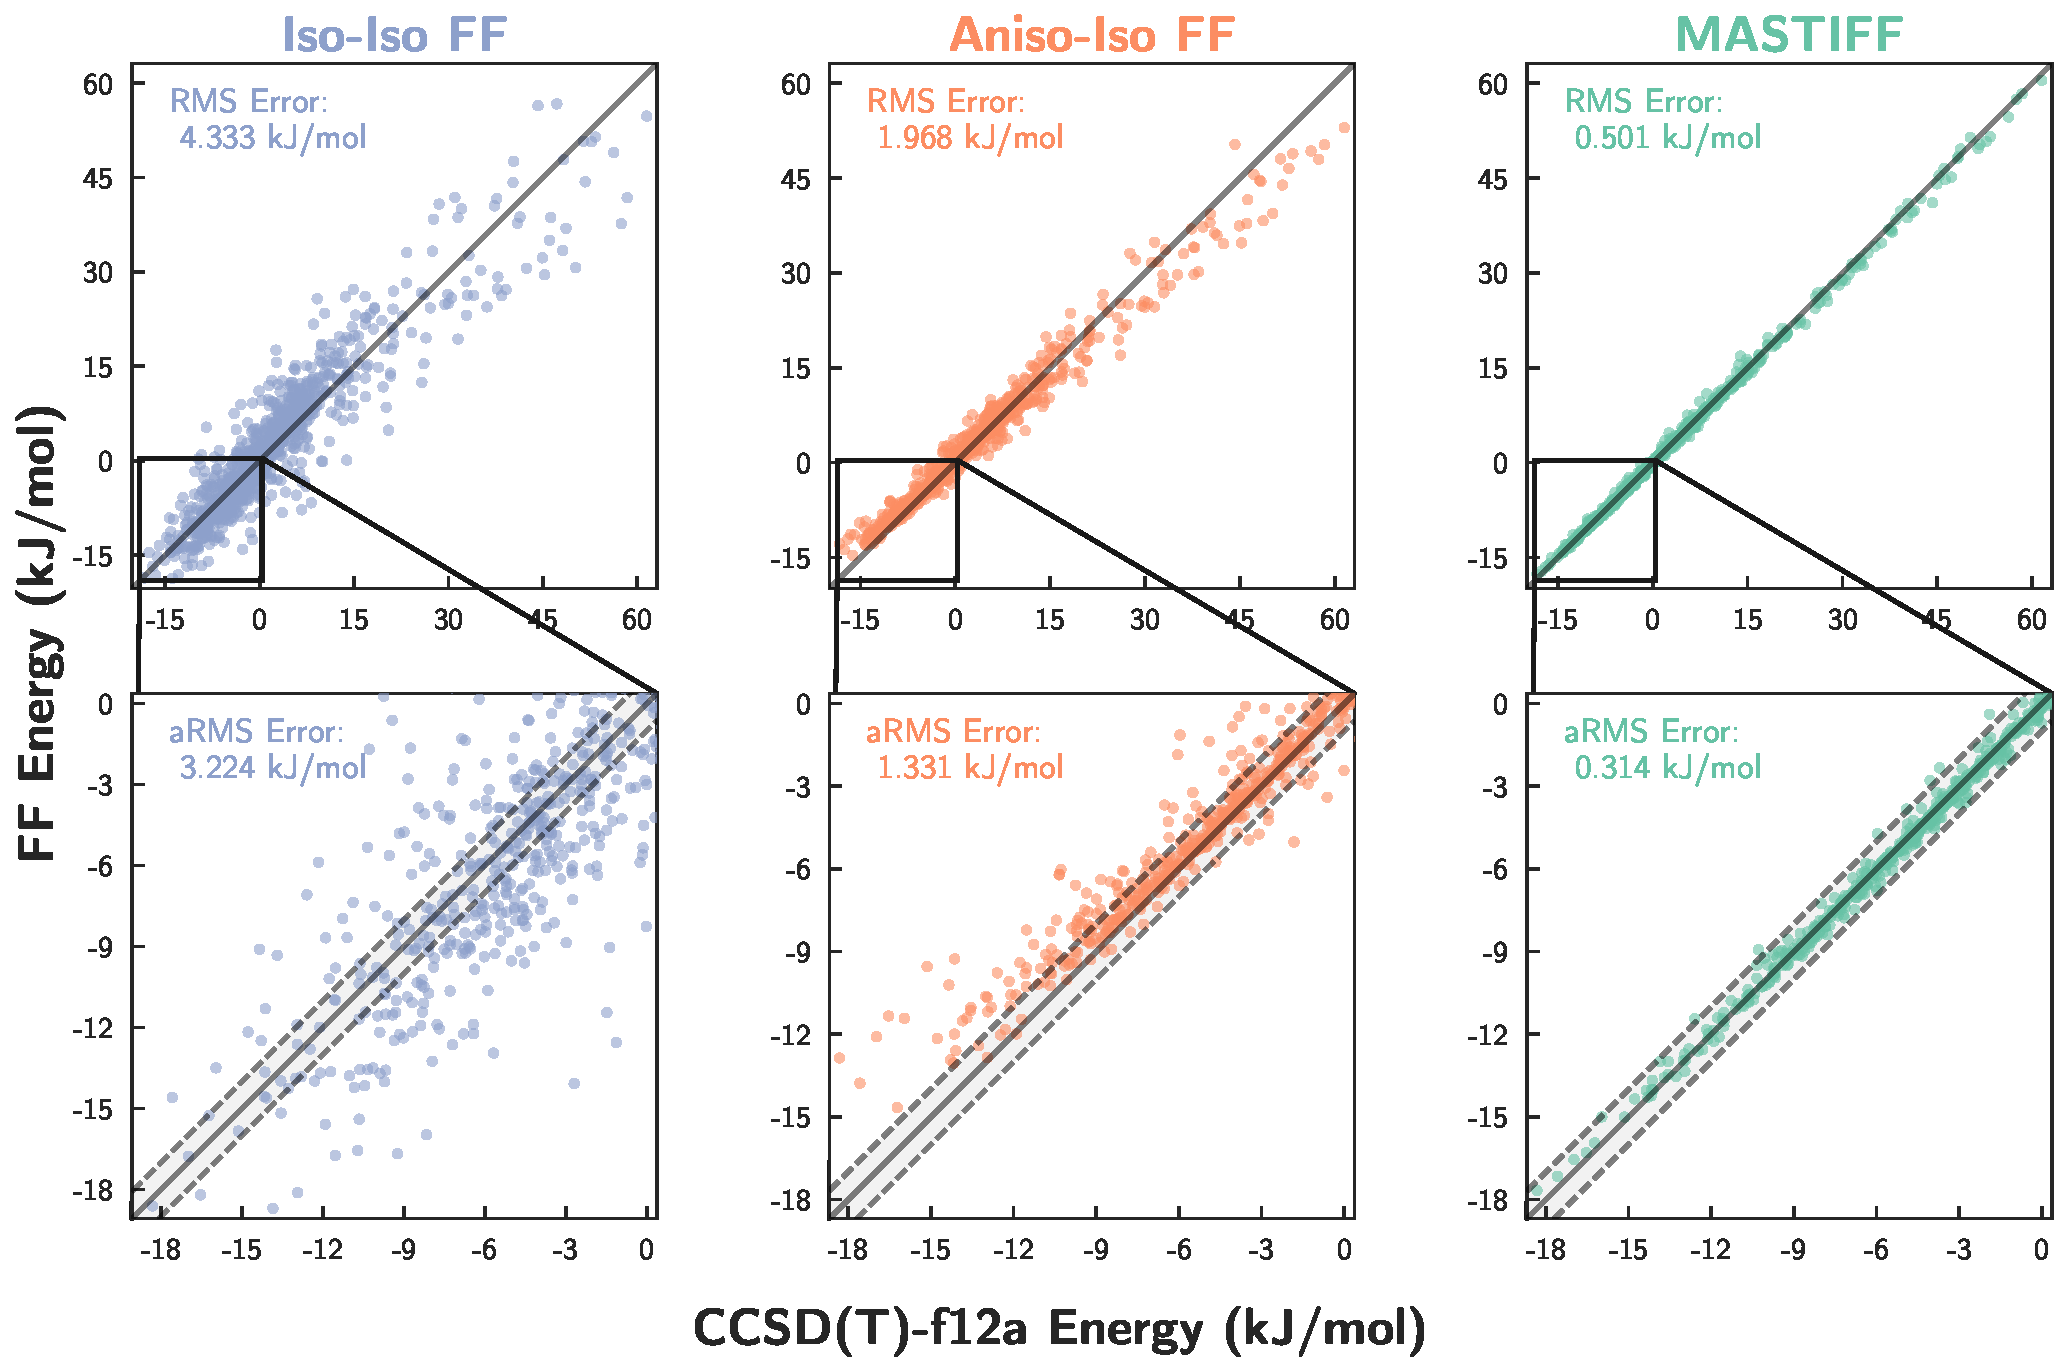
\includegraphics[width=0.9\textwidth]{anisotropic/scatterplots/h2o_h2o_comparison.pdf}
    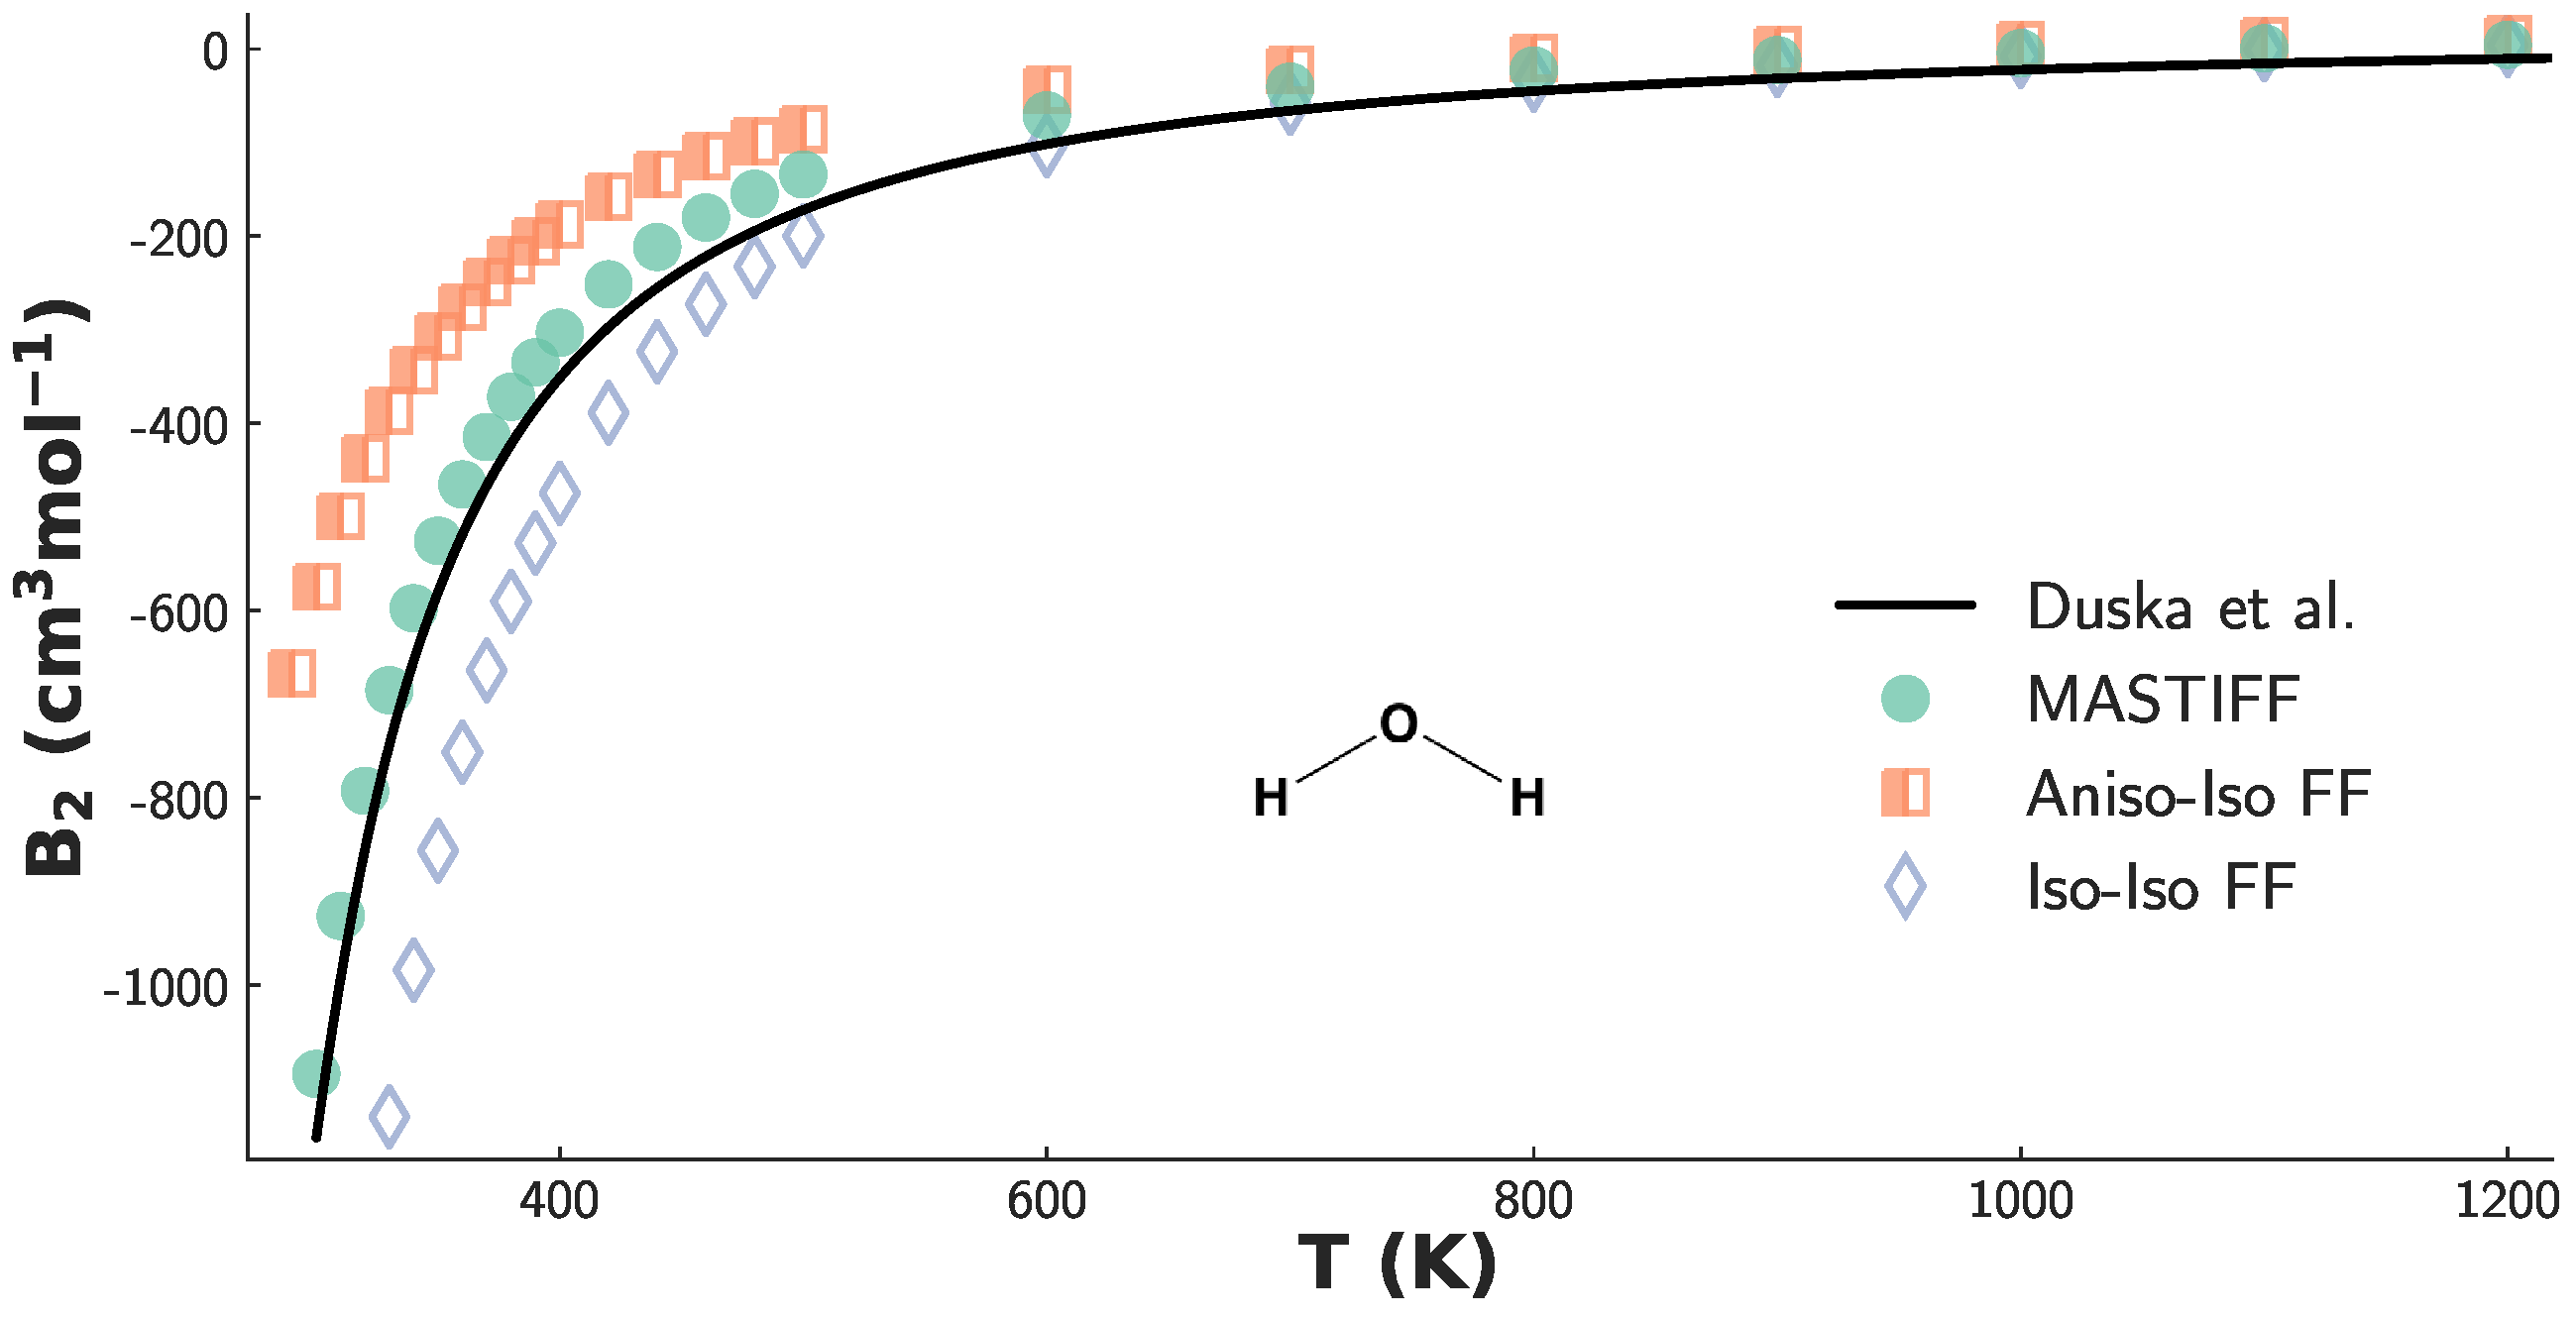
\includegraphics[width=0.9\textwidth]{anisotropic/virials/h2o/h2o_2nd_virial.pdf}
    \caption{
        Classical second virial for water. Experimental data from
            \citen{Duska2013}. 
        Note that some data points from \isoff extend below the plot area.
            }
    \label{fig:h2o_virial}
    \end{figure}
    %%%%%%%%%%%% H2O Comparison %%%%%%%%%%%%%
    %%%%%%%%%%%% H2O Comparison %%%%%%%%%%%%%
    \begin{figure}[ht]
    \centering
    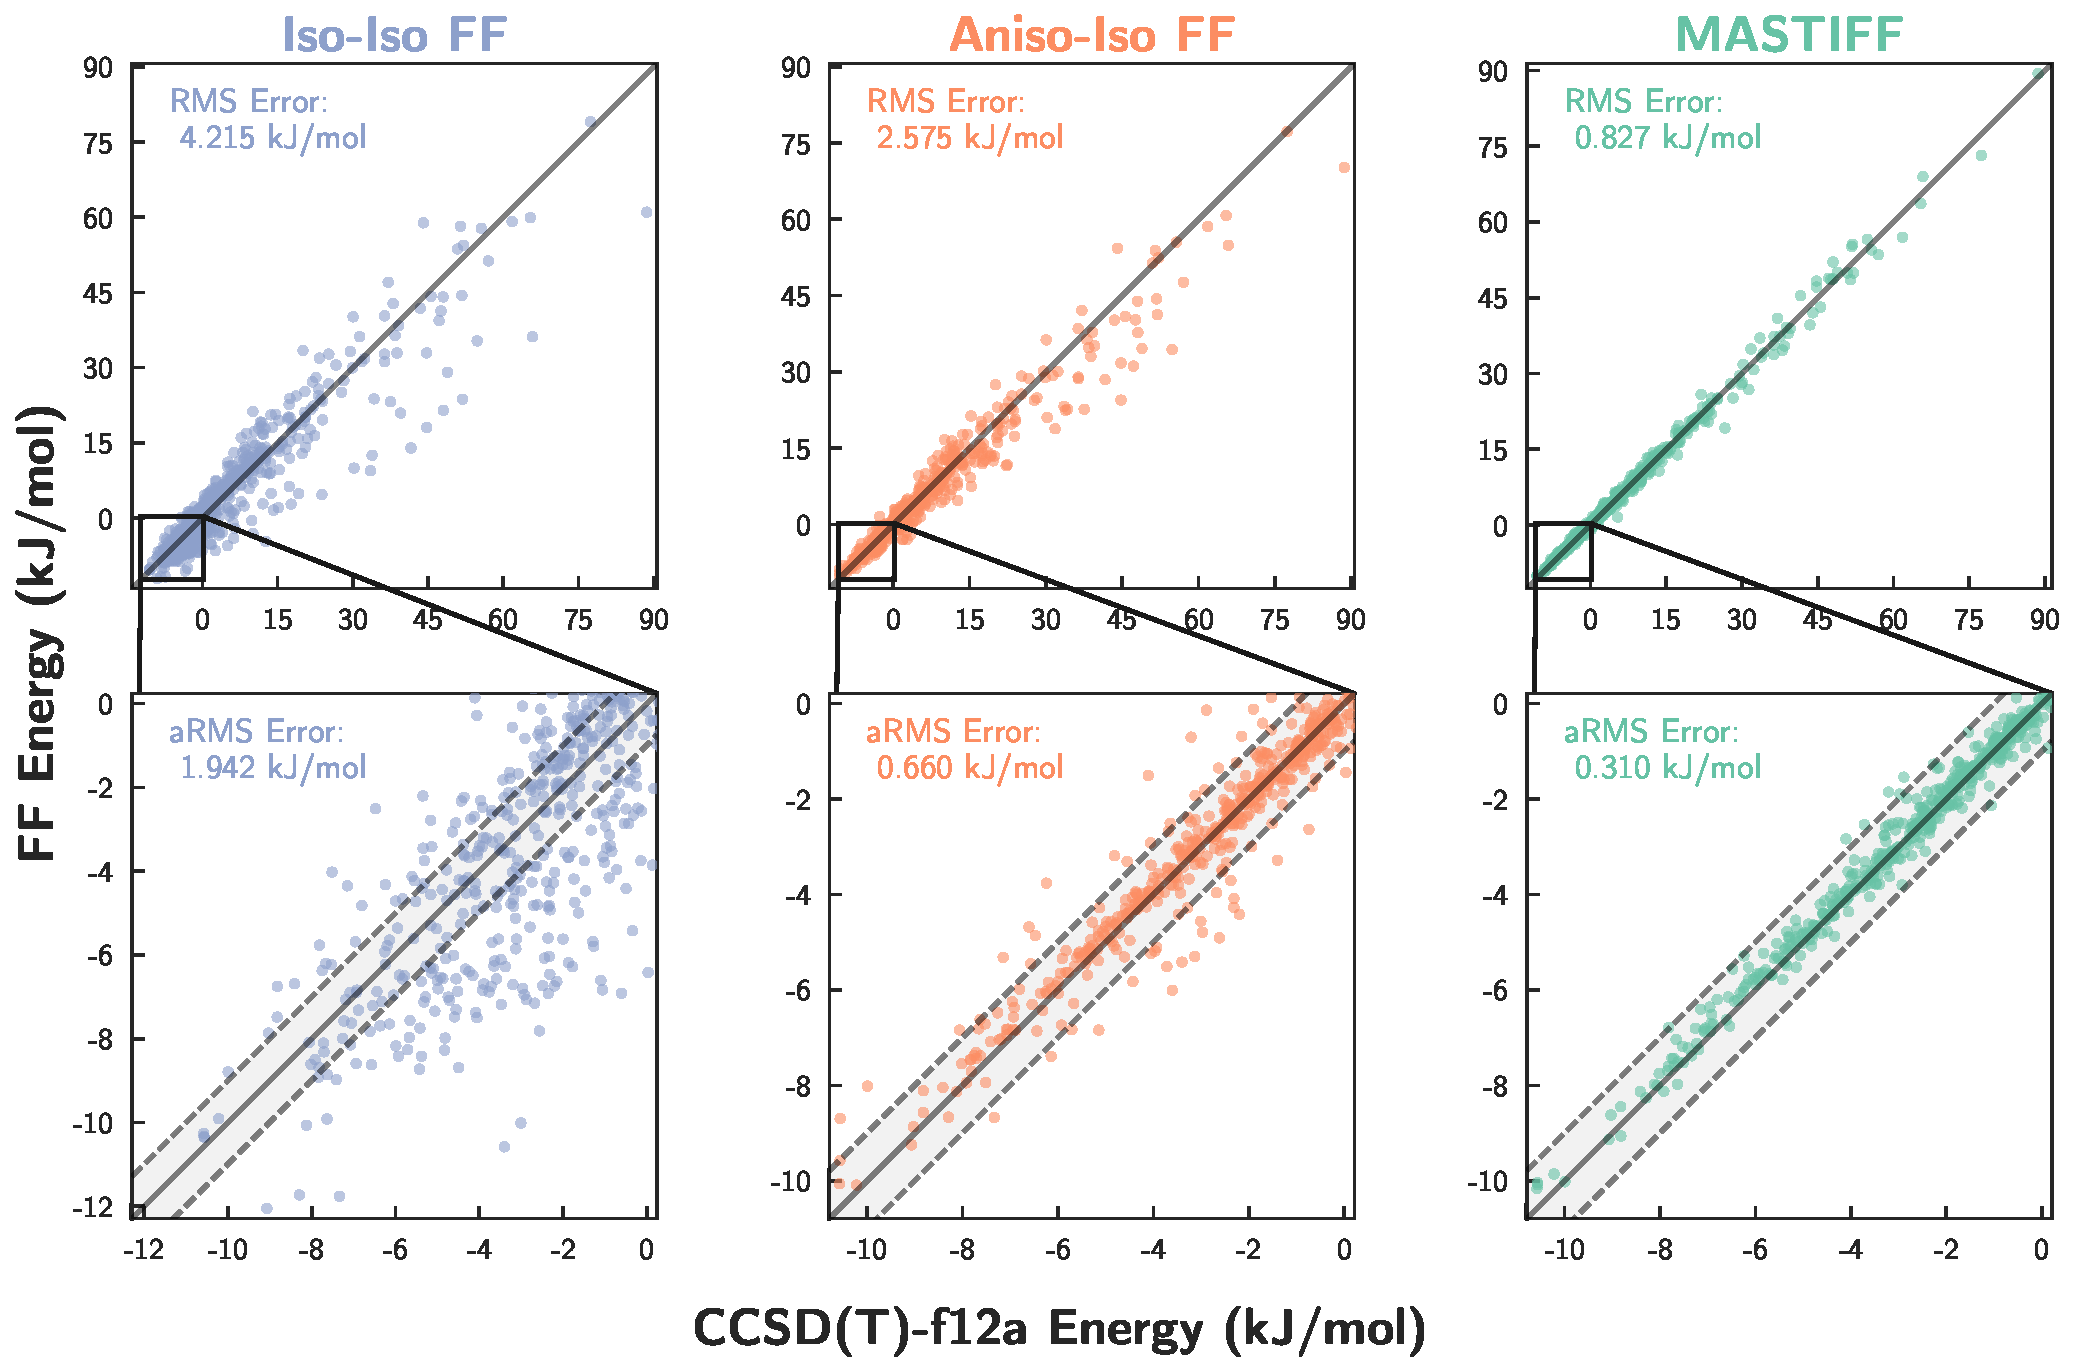
\includegraphics[width=0.9\textwidth]{anisotropic/scatterplots/nh3_nh3_comparison.pdf}
    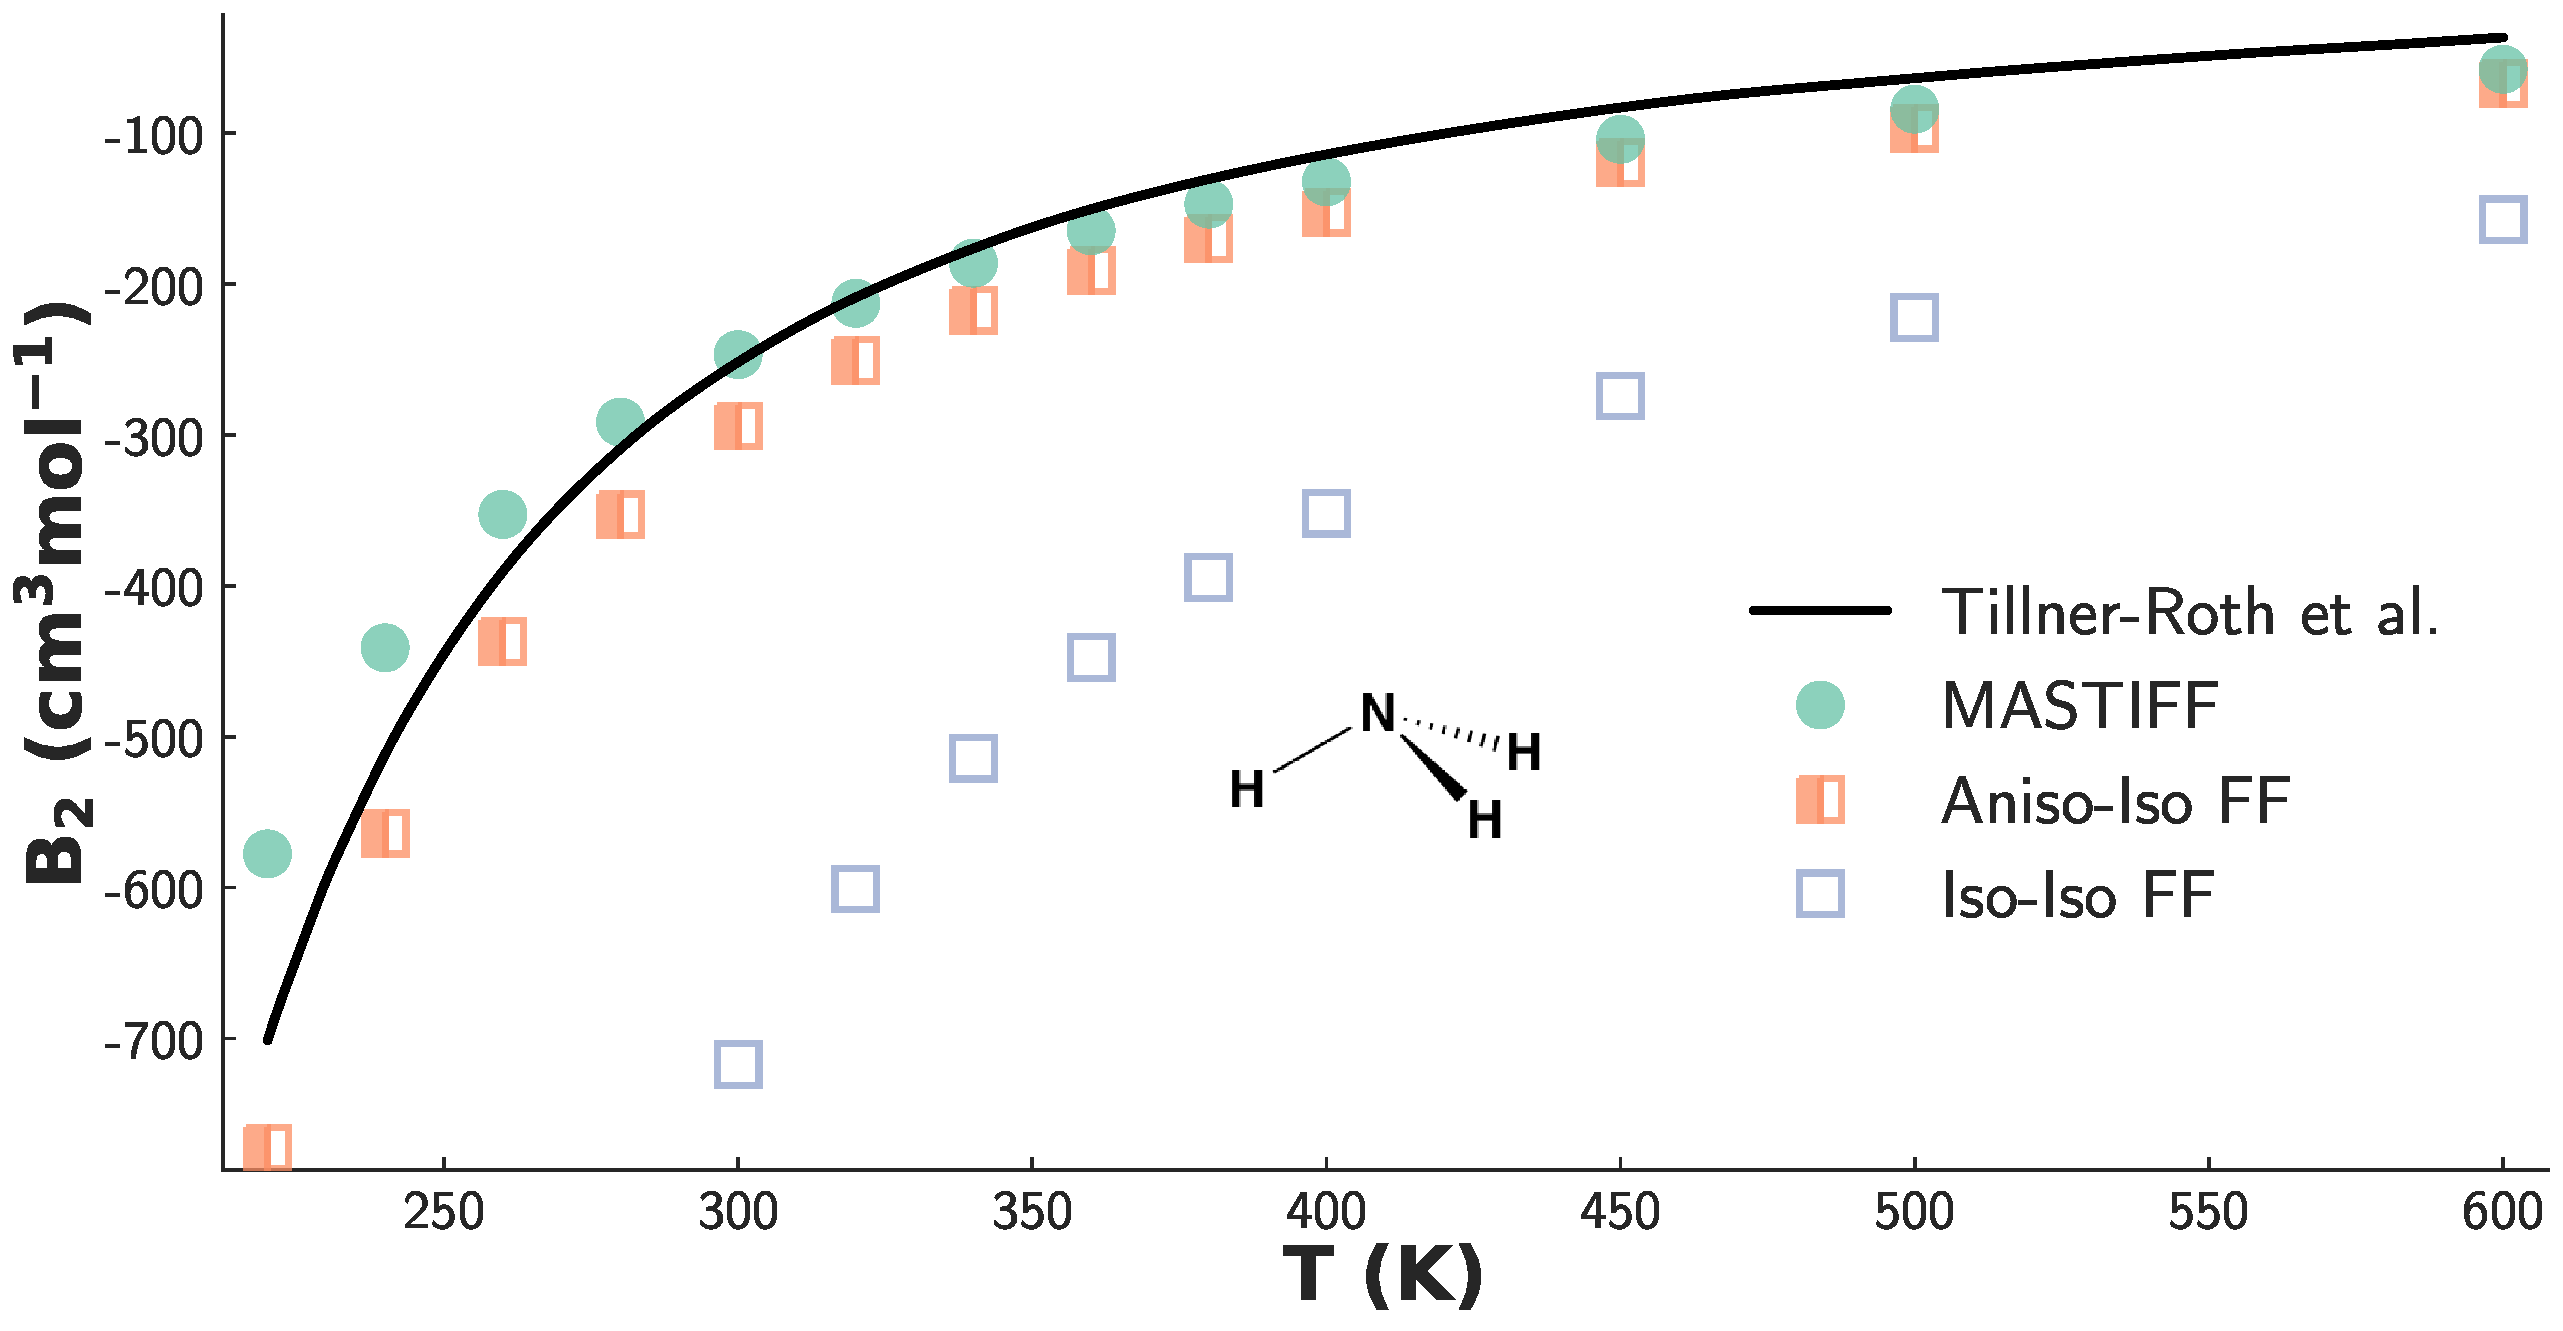
\includegraphics[width=0.9\textwidth]{anisotropic/virials/nh3/nh3_2nd_virial.pdf}
    \caption{
        Classical second virial for ammonia. Experimental data from
            \citen{tillner1993neue}.
        Note that some data points from \isoff extend below the plot area.
            }
    \label{fig:nh3_virial}
    \end{figure}
    %%%%%%%%%%%% H2O Comparison %%%%%%%%%%%%%
    %%%%%%%%%%%% H2O Comparison %%%%%%%%%%%%%
    \begin{figure}[ht]
    \centering
    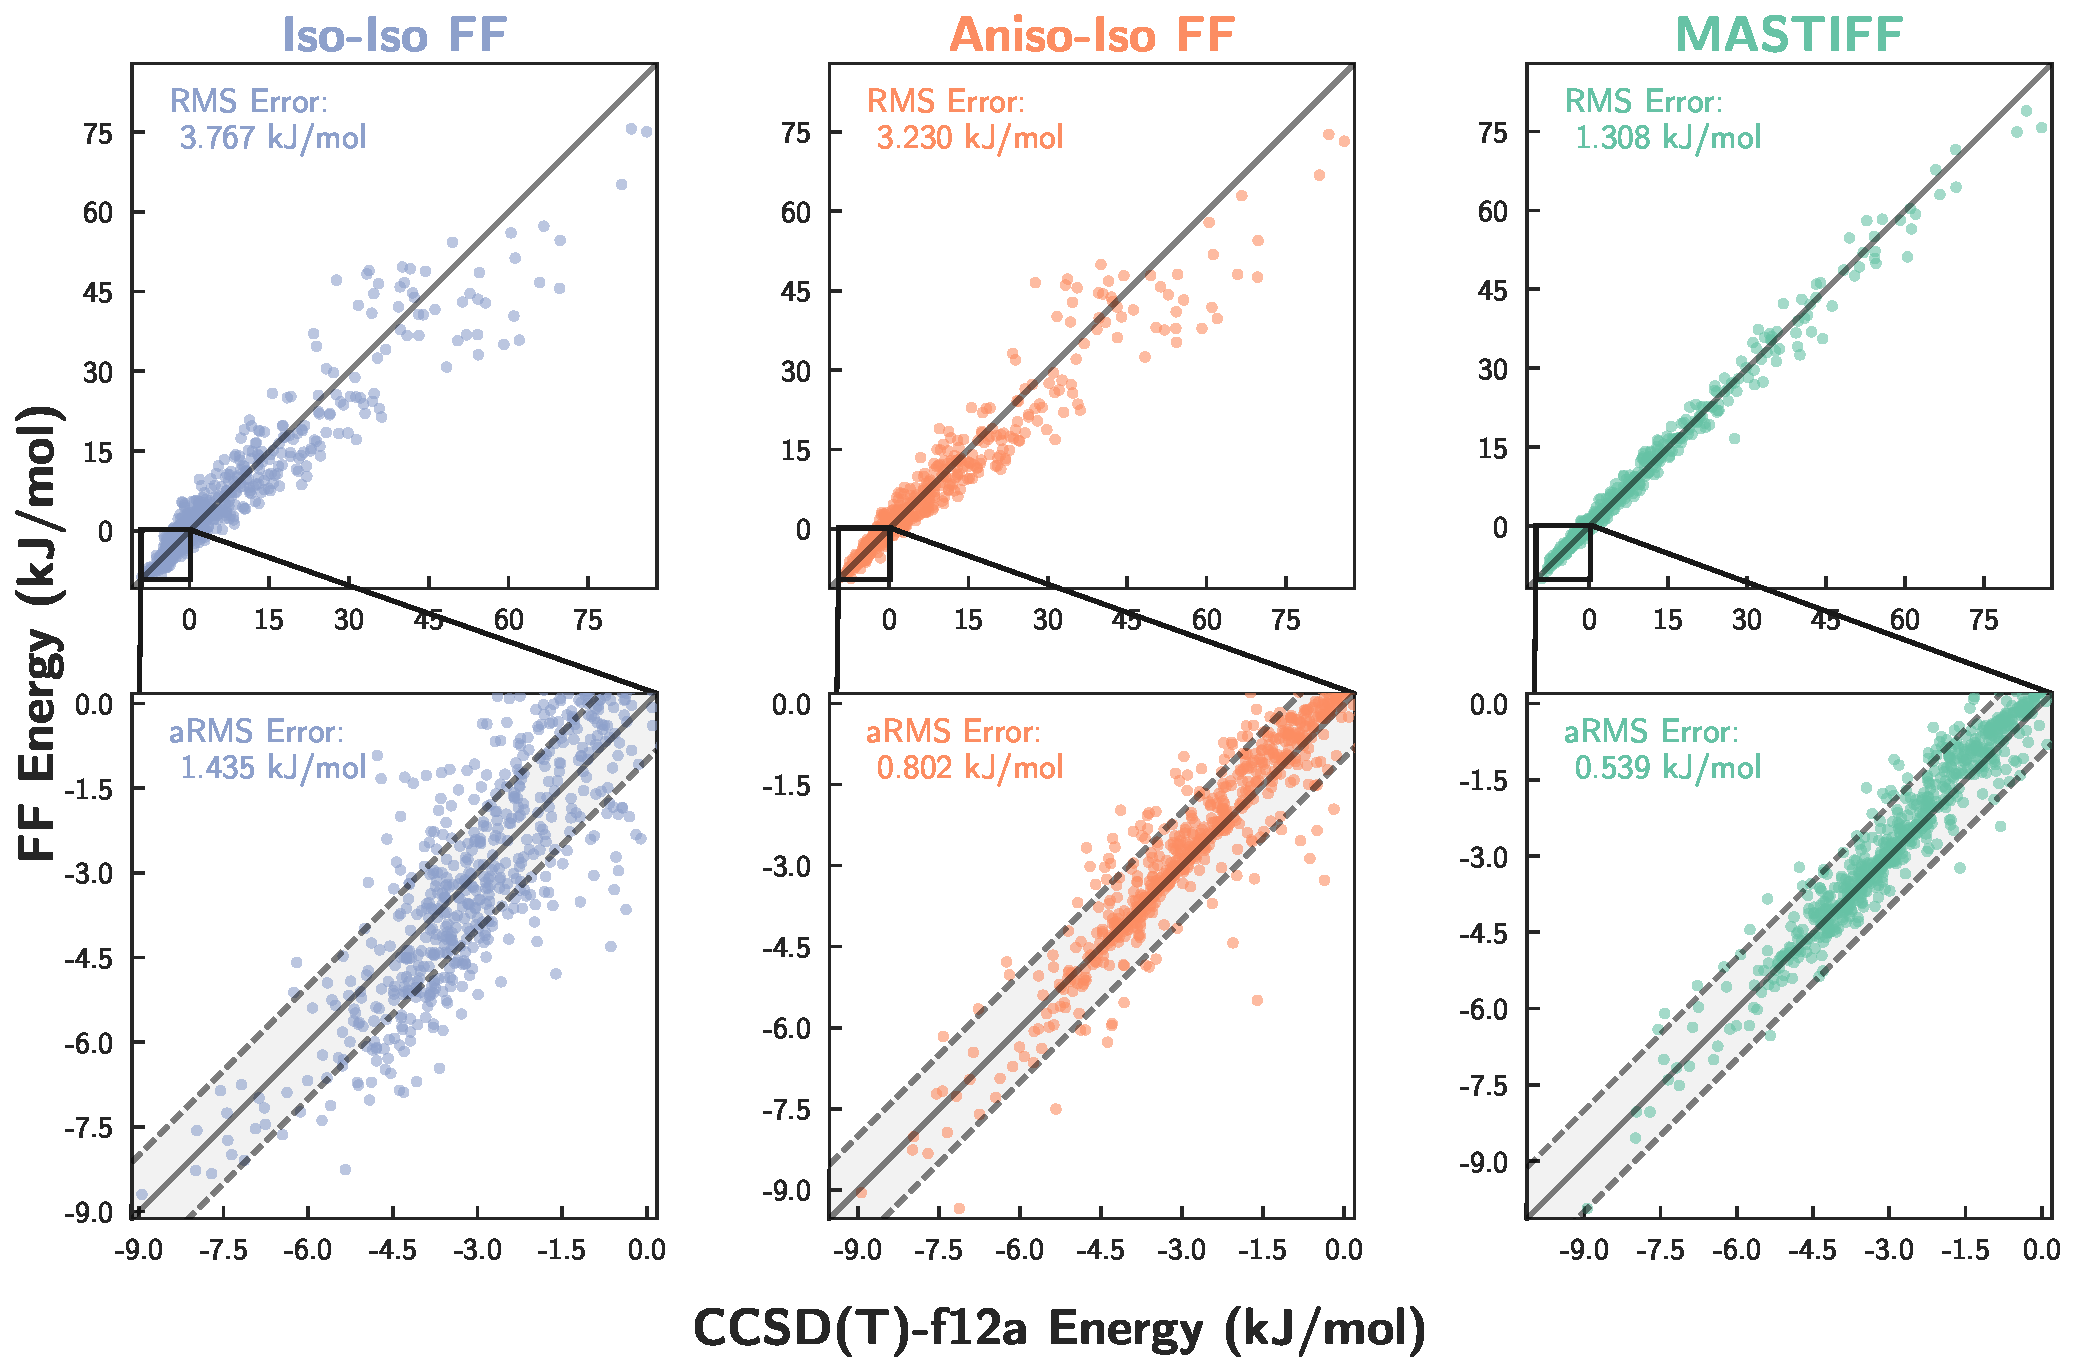
\includegraphics[width=0.9\textwidth]{anisotropic/scatterplots/chloromethane_chloromethane_comparison.pdf}
    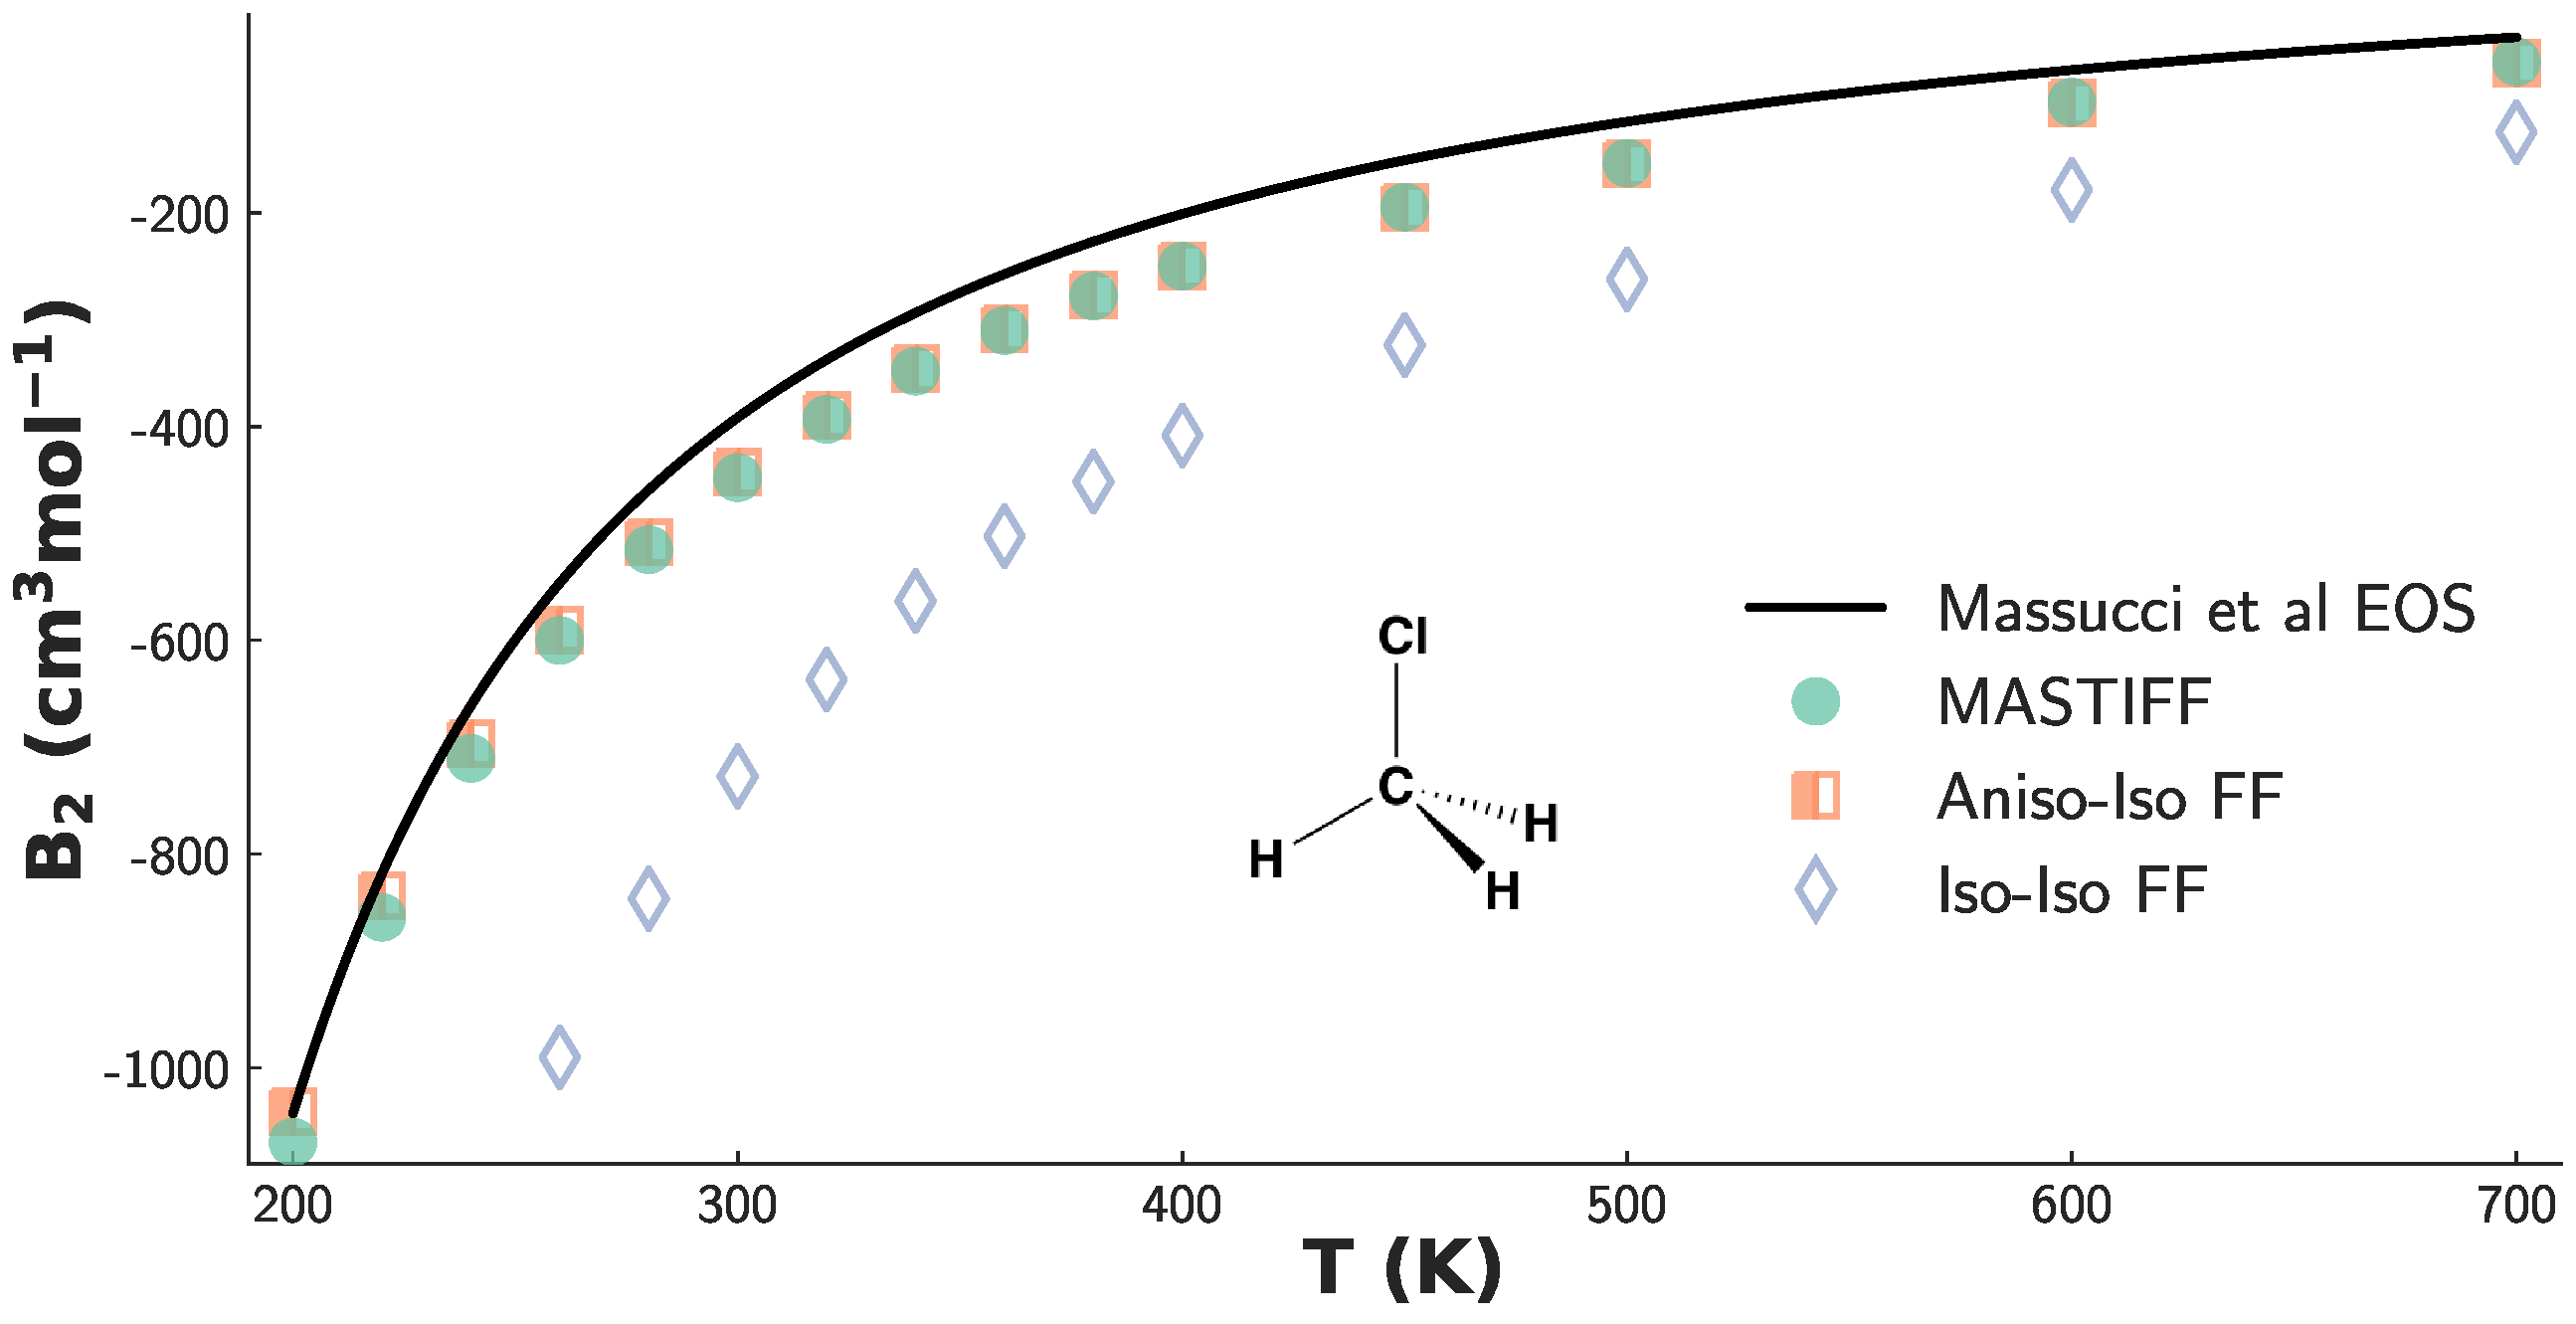
\includegraphics[width=0.9\textwidth]{anisotropic/virials/chloromethane/chloromethane_2nd_virial.pdf}
    \caption{
        Classical second virial for chloromethane. Experimental equation of
        state (EOS) from \citen{Massucci1998}.
        Note that some data points from \isoff extend below the plot area.
            }
    \label{fig:chloromethane_virial}
    \end{figure}
    %%%%%%%%%%%% H2O Comparison %%%%%%%%%%%%%
    %%%%%%%%%%%% Virial for CO2 %%%%%%%%%%%%%
    \begin{figure}[ht]
    \centering
    \includegraphics[width=0.9\textwidth]{anisotropic/scatterplots/co2_co2_comparison.pdf}
    \includegraphics[width=0.9\textwidth]{anisotropic/virials/co2/co2_2nd_virial.pdf}
    \caption{
        Classical second virial for \co. 
        Experimental data from \citen{Span1996}
            }
    \label{fig:co2_virial}
    \end{figure}
    %%%%%%%%%%%% Virial for CO2 %%%%%%%%%%%%%
%
First,
we find that the \mastiff-CC
methodology predicts virial coefficients
which closely corresponds to experimental data. Given the range of systems
tested (\co dimer interactions are dispersion dominated, while \cl, \nh, and
\ho have relatively larger electrostatic and polarization contributions), 
this suggests that, when benchmarked against high-quality electronic structure
theory, our anisotropic methodology offers a general strategy for
quantitatively accurate
pairwise potential development. Second, we note that
the \isoff-CC 
predictions are much worse than their \mastiff-CC or \isaff counterparts, 
suggesting that
an accurate treatment of long-range electrostatics is essential to obtain
accurate virial coefficients.
Finally, though \isaff-CC gives equally good predictions for some systems
(notably \cl) compared to the \mastiff-CC method, 
virial coefficients for other systems (especially \ho) are less
accurate, suggesting that dispersion and short-range
anisotropies are also important in many systems for the accurate prediction of
virial coefficients. Consequently, and in summary, 
the minimal additional computational overhead (compared to \isaff-CC) and
excellent accuracy of \mastiff-CC permits us to recommend this fully anisotropic \mastiff methodology 
for the prediction of dimer interaction energies and second virial coefficients.


\clearpage
\end{subsection}
\begin{subsection}{Comparison to Experiment: Condensed Phase Properties of \co}
\label{sec:co2}

To demonstrate the applicability of the \mastiff methodology in condensed
phase simulation, we have developed a complete
many-body potential for \co, and have run bulk simulations involving a variety
of vapor, liquid, supercritical, and solid phase points for preliminary
comparisons to experiment.  As above, we use the \mastiff-CC
potential to describe the pairwise potential and the many-body induction.
As for other many-body effects, it
is well-known\cite{Yu2012b,Hellmann2017,Oakley2009a} that three-body
dispersion, and to a lesser extent, three-body exchange, are also
important.\cite{Desgranges2015} 
Thus, 
%% after testing a few combination-rule
%% compatible (so as to be easily
%% implemented in OpenMM) three-body potentials for their ability to reproduce the
%% \citeboth{Hellmann2017} three-body interaction energy database, 
we model three-body dispersion via a modified version of the three-body dispersion potential developed by
\citeauthor{Oakley2009a} (see \cref{sec:methods}).  Three-body exchange
effects are not accounted for in our model, however 
prior work shows they are very small under the conditions studied
here.\cite{Yu2012b}

Density predictions for the vapor, liquid, and supercritical phases of \co are
shown in \cref{tab:densities}, and enthalpies of
sublimation and vaporization are shown in \cref{tab:deltah}. 
%
We find it notable and highly encouraging that
\mastiff-CC reproduces \emph{all} studied experimental properties to within a
few percent. Of particular note is our excellent reproduction of the
sublimation enthalpy, which critically depends on the lattice energy of the
solid phase. Unlike with liquid or supercritical \co, where
many dimer configurations are sampled,
the
solid consists of only four symmetry-unique
configurations. Consequently, whereas an isotropic
potential (which is in error for particular dimer
configurations, but can take advantage of error cancellation to be accurate in an average sense) 
might yield good property predictions for the liquid phase, 
it would not be expected to correctly predict the solid phase (where beneficial
error cancellation is unlikely). 
Indeed, most theories (including our previously developed SYM-3B
model,\cite{Yu2012b} nearly all popular empirically-developed \co
models,\cite{Perez-Sanchez2013} AMOEBA,\cite{Heit2016a} and many electronic
structure theories\cite{Heit2016a}) struggle to correctly predict the solid phase
properties of \co! For this reason, 
the enthalpy of sublimation is
an extremely stringent test of force field
quality,\cite{Perez-Sanchez2013} 
and our accurate reproduction
of this quantity is evidence for both the excellent quality of the \mastiff-CC
potential in specific and of the importance of atomic-level anisotropy in
general.
Though more testing is needed to confirm
the accuracy of our anisotropic force field for
other phase points, our results suggest that, crucially, the
\mastiff-CC potential is transferable across the entire phase diagram of
molecular \co, and is capable of describing the gas, liquid, supercritical,
and solid phases. 

Despite the excellent success of the \mastiff-CC model, it is also worthwhile to
address and understand its minor shortcomings. In particular, we have studied 
representative two- and three-body energies taken from a snapshot of
the liquid at 273.15 K and 100 bar. For the two-body energies, we have compared
against the extremely accurate \citeboth{Kalugina2014} potential, while for
three-body energies we have benchmarked against the \citeboth{Hellmann2017}
PES. From these results (\cref{sec:mastiff-co2_snapshots}), 
it is clear that our pairwise
\mastiff potential is highly accurate for all configurations present in the
liquid, with very small \rmse and no systematic error in the
potential, such that the total two-body energy is accurate to within 0.05\%
compared to the \citeauthor{Kalugina2014} PES. Once again, this result argues
strongly for the accuracy and transferability of the \mastiff methodology, and
suggests that an inclusion of anisotropy is essential, not only for gas-phase
clusters, but also for simulations of the bulk. By contrast, our three-body
potential is systematically in error compared to the \citeauthor{Hellmann2017}
PES. Though some of this error may be due to inaccuracies in the
benchmark potential itself as compared to coupled-cluster,\cite{Hellmann2017}
most of this error is likely due to
inaccuracies in our model for many-body \co interactions. The
atomically-isotropic treatment of three-body dispersion, neglect of
higher-order dispersion terms ,
and neglect of explicit three-body exchange
may all contribute to this error, and
an improved model for many-body \co interactions will be the subject of future
research. Indeed, it is well-known that the density can be extremely sensitive
to the treatment of many-body effects,\cite{Desgranges2015} and it is highly
probable that an improved many-body model would reduce the already small
errors observed in our \mastiff-CC predictions.
Regardless, for now we conclude that, despite some small residual errors
arising from the simplified treatment of many-body effects, our \mastiff-CC
methodology yields for an extremely accurate force field for \co with
applicability across 
a range of experimentally-important phases.



%%%%%%%%%%%%%%%%%%%%% Macroscopic Properties %%%%%%%%%%%%%%%%%%%%%%%%%%%%%%%%%%
\begin{table}
%\small
\centering
\renewcommand\arraystretch{1.1}
\begin{tabular}{@{}lccccc@{}}
\hline
\toprule

Phase & T (K) & P (bar) &  Density (g/ml) &  Exp. & \% Error  \\

\midrule
Gas       & 300    &  50  & 0.131   & 0.128 &  2.34  \\
Supercritical & 320    & 140  & 0.728   & 0.703 &  3.56  \\
Liquid    & 300    & 100  & 0.825   & 0.802 &  2.87  \\
Liquid    & 273.15 & 100  & 1.000   & 0.974 &  2.67  \\
%
\bottomrule
\hline
\end{tabular}
\caption{
    Select densities for \co across a range of experimental conditions.
    Experimental data taken from the EOS of \citen{Span1996}.
    Entries ordered by increasing experimental density.
	}
\label{tab:densities}
\end{table}
%\normalsize
%%%%%%%%%%%%%%%%%%%%% Macroscopic Properties %%%%%%%%%%%%%%%%%%%%%%%%%%%%%%%%%%


%%%%%%%%%%%%%%%%%%%%% Macroscopic Properties %%%%%%%%%%%%%%%%%%%%%%%%%%%%%%%%%%
\begin{table}
%\small
\centering
\renewcommand\arraystretch{1.1}
\begin{tabular}{@{}lccccc@{}}
\hline
\toprule

Phases & T (K) & \deltah (\kjmolold) &  Exp. & \% Error  \\

\midrule
s $\to$ g   & 194.76 & $25.0 \pm 0.15$ &  25.2  &  -0.8  \\
l $\to$ g   & 288    & 7.92   &    7.80    &   -1.4 \\
%
\bottomrule
\hline
\end{tabular}
\caption{
    Enthalpies of vaporization/sublimation for \co at several temperatures. 
    Experimental data taken from the EOS of \citen{Span1996}.
    The uncertainty in the enthalpy of sublimation is due to ambiguity in the theoretical zero-point energy for \co (see
    \cref{sec:methods}. 
	}
\label{tab:deltah}
\end{table}
%\normalsize
%%%%%%%%%%%%%%%%%%%%% Macroscopic Properties %%%%%%%%%%%%%%%%%%%%%%%%%%%%%%%%%%



\end{subsection}



%% Explain MSE Fits
%%     Exchange:
%%     Electrostatics:
%%     Dispersion: 
%%     Total Energy:



\end{section}
%%%%%%%%%%%%%%%%%%%%%%%%%%%%%%%%%% Results %%%%%%%%%%%%%%%%%%%%%%%%%%%%%%%%%%%%%%%%





%%%%%%%%%%%%%%%%%%%%%%%%%%%%% Conclusions %%%%%%%%%%%%%%%%%%%%%%%%%%%%%%%%%%%%%%%%%
\begin{section}{Conclusions and Recommendations}
\label{sec:conclusions}

We have developed a comprehensive methodology for modeling 
atomic-level anisotropy in standard intermolecular force fields. 
By treating this anisotropy through a simple extension of
standard isotropic force
fields,\cite{VanVleet2016}
%% and by accounting for this anisotropy in our models for each
%% electrostatics, exchange-repulsion, induction, and dispersion,
we have 
successfully demonstrated how this computationally-efficient treatment of atomic-level anisotropy leads to
significant improvements in models for intermolecular interactions.
Critically, 
and in contrast to popular assumption, we have shown how the accurate treatment of multipolar electrostatics 
does not \emph{by itself} account for all energetically-important effects of
atomic-level anisotropy.
Rather, our results indicate that anisotropy may need to be included in the
each electrostatic, exchange and dispersion terms in order to obtain intermolecular
force fields of the highest quality.
In the present study,
and in agreement with the more quantitative metrics proposed by others,\cite{Wheatley2012,Kramer2014} 
we have found
a comprehensive model of atomic-level anisotropy to be particularly important for obtaining sub-\kjmolold
accuracy for describing molecules with heteroatoms
(particularly ones with exposed lone pairs), carbons in multiple
bonding environments, and hydrogens bound to anisotropic heavy atoms. 
Our new intermolecular `\mastiff' force fields show great promise, not only with
respect to high-quality electronic structure benchmark energies, but also with
respect to experimental property predictions.
Importantly, \mastiff maintains high efficiency and transferability.
and can easily be implemented in common software packages such as 
OpenMM for use in condensed phase simulations.\cite{Eastman2013} 

Despite the advances presented in this Chapter, several aspects of our force
field methodology require further improvement, and will be the subject of
ongoing research. In particular, an improved description of induction effects
will become essential for accurate bulk simulations of highly polarizable
molecules such as water.  We are now actively working to develop improved
models that can describe both long-range anisotropic polarization and
short-range polarization damping, as these aspects of the force field
critically affect both the two- and many-body induction energies and
can account for a sizable fraction of the total interaction energy in
condensed phases.
We anticipate that these improved models for induction will, in
combination with an accurate description of three-body dispersion and
exchange, yield a general approach to force field development that captures
both the two- and many-body features of intermolecular interactions, in turn
enabling highly accurate, `next-generation' force field development capable of
simulating a wide array of phases and chemical environments.



\end{section}
%%%%%%%%%%%%%%%%%%%%%%%%%%%%% Conclusions %%%%%%%%%%%%%%%%%%%%%%%%%%%%%%%%%%%%%%%%%


\begin{subappendices}
%%%%%%%%%%%%%%%%%%%%%%%%%%%%% Appendix %%%%%%%%%%%%%%%%%%%%%%%%%%%%%%%%%%%%%%%%%%%%
\begin{section}{Motivation for \gij}
\label{sec:appendix}

As shown elsewhere,\cite{Stone1978,Stone1984}
an exact (under the ansatz of
radial and angular separability) model for \gij is given by Stone's $\bar{S}$-functions, 
which form a complete basis set for describing any scalar function which
depends on the relative orientation
between molecules, and are given (following Stone's
notation\cite{stone2013theory}) by the formula
% General s-function
\begin{align}
%
\bar{S}^{k_1 k_2}_{l_1 l_2 j} = 
i^{l_1 - l_2 -j}
\begin{pmatrix} l_1 & l_2 & j \\ 0 & 0 & 0 \end{pmatrix}^{-1}
\sum \limits_{m_1 m_2 m} 
[D^{l_1}_{m_1 k_1}(\Omega_1)]^*
[D^{l_2}_{m_2 k_2}(\Omega_2)]^*
C_{lm}(\theta,\phi)
\begin{pmatrix} l_1 & l_2 & j \\ m_1 & m_2 & m \end{pmatrix}.
%
\end{align}
The general form of these $\bar{S}$-functions can be quite complicated, and
involve both the Wigner $D$ rotation matrices and Wigner $3j$-symbols (quantities
in parentheses) as well as the degree ($l_1$, $l_2$, and $j$) and order
($m_1$, $m_2$, and $m$ for the global coordinate system, $k_1$ and $k_2$ for the
various local coordinate systems) of the spherical harmonic tensors. Here
subscripts reference either molecule 1 or molecule 2, and subscriptless
quantities refer to the dimer as a whole.

In order to obtain a functional form for the exchange-repulsion that is
amenable to simple combination rules (a necessary prerequisite for
transferable potentials), we must somehow be able to separate \gij into monomer
contributions. Unfortunately, many of the \sfunc depend on the relative
orientation of the dimer itself, and thus must be excluded in the development
of \emph{transferable} potentials.
Thus as a second ansatz (empirically validated by us in \cref{sec:results} and by
others\cite{Millot1992})
we neglect all contributions from \sfunc that depend
on both local coordinate systems. This leaves us with two sets of \sfunc, namely
%
\begin{align}
\bar{S}^{k0}_{l0l} = C_{lk}(\theta_i,\phi_i)
\end{align}
%
and
%
\begin{align}
\bar{S}^{0k}_{0ll} = C_{lk}(\theta_j,\phi_j)
\end{align}
%
which are simply the renormalized spherical harmonics (\cref{eq:sph_harm})
expressed in each of the two local coordinate systems.

Given our truncated expressions for the \sfunc, we now need only extend our
functional form for \fij to incorporate these anisotropic contributions.
We choose, in a manner analogous to literature precedent,
\cite{Stone2007,Mitchell2001,Price2000,Stone1988,Day2003,Torheyden2006,Totton2010,Misquitta2016,Price2010a}
to expand the \Aex{i} and \Aex{j} parameters of \cref{eq:aij} in terms of a truncated
expansion of \sfunc. 
(In principle, we could also account for anisotropy in the \B parameters of
our model for \fij. However, previous literature suggests that in practice this `hardness'
parameter can often be treated as constant, and we also neglect its possible
anisotropy in this Chapter.) 
Consequently, all short-range anisotropies are modeled in this Chapter
by the expressions given in \cref{eq:gij} and \cref{eq:vex}.

%% Finally, and as with exchange-repulsion, molecular anisotropic long-range
%% dispersion coefficients can be determined from an \sfunc expansion of the form
%% %
%% \begin{align}
%% \vdisp = - \sum\limits_{l_A l'_A l_B l'_B}
%%            \sum\limits_{L_A L_B J K_A K_B}
%%             \bar{C}_n(L_A L_B J; K_A K_B)R^{-n} S^{K_A K_B}_{L_A L_B J}
%% \end{align} 
%% %


\end{section}
%%%%%%%%%%%%%%%%%%%%%%%%%%%%% Appendix %%%%%%%%%%%%%%%%%%%%%%%%%%%%%%%%%%%%%%%%%%%%
%% \documentclass[12pt,letterpaper]{article}
%% \usepackage[margin=1in,bottom=1in]{geometry} % see geometry.pdf on how to lay out the page. There's lots.
%% 
%% \usepackage{hyperref}
%% \usepackage[journal=jacs]{chemstyle} %Other chemical formatting
%% \usepackage{chemscheme} % Chemical graphics
%% \usepackage{chemcompounds}
%% \usepackage{caption}
%% \usepackage{bpchem} % Chemical compounds
%% \usepackage{setspace}
%% \usepackage{fullpage}
%% \usepackage{graphicx}
%% \usepackage{xspace}
%% \usepackage{booktabs}
%% \usepackage{pdflscape}
%% \usepackage[sort&compress,numbers,super]{natbib}
%% \usepackage{bibentry}
%% %\usepackage{xr}
%% %\externaldocument{isa_ff}
%% \usepackage{amsmath}
%% \usepackage{longtable}
%% \usepackage{xfrac}
%% \usepackage{multirow}
%% \usepackage{dcolumn}
%% \usepackage{siunitx}
%% \usepackage{subcaption}
%% 
%% %eqref
%% \usepackage{letltxmacro}
%% \LetLtxMacro{\originaleqref}{\eqref}
%% \renewcommand{\eqref}{eq.~\originaleqref}
%% \newcommand{\Eqref}{Eq.~\originaleqref}
%% 
%% %figref
%% \newcommand{\figref}[1]{Figure~\ref{#1}}
%% \newcommand{\tabref}[1]{Table~\ref{#1}}
%% \newcommand{\secref}[1]{Section~\ref{#1}}
%% 
%% \newcommand{\super}[1]{\textsuperscript{#1}}
%% \newcommand{\sub}[1]{\textsubscript{#1}}
%% \renewcommand{\thefootnote}{\fnsymbol{footnote}}
%% \newcommand{\ra}[1]{\renewcommand{\arraystretch{#1}}}
%% \newcommand{\centercell}[1]{\multicolumn{1}{C}{#1}}
%% 
%% % Supplementary Information Labels
%% \newcommand{\beginsupplement}{%
%%         \setcounter{table}{0}
%%         \renewcommand{\thetable}{S\arabic{table}}%
%%         \setcounter{figure}{0}
%%         \renewcommand{\thefigure}{S\arabic{figure}}%
%%         \setcounter{section}{0}
%%         \renewcommand{\thesection}{S\arabic{section}}%
%%      }
%% 
%% \newcommand{\citeboth}[1]{\citeauthor{#1}\cite{#1}\xspace}
%% \newcommand*{\citen}[1]{%
%%   \begingroup
%%     \romannumeral-`\x % remove space at the beginning of \setcitestyle
%%     \setcitestyle{numbers}%
%%     ref. \cite{#1}%
%%   \endgroup   
%% }
%% 
%% \hyphenation{homodimer}
%% 
%% 
%% % ISA-FF Paper lingo
%% 
%% \newcommand{\co}{\BPChem{CO\_2}\xspace}
%% \newcommand{\ho}{\BPChem{H\_2O}\xspace}
%% \newcommand{\nh}{\BPChem{NH\_3}\xspace}
%% \newcommand{\cl}{\BPChem{CH\_3Cl}\xspace}
%% 
%% 
%% \newcommand{\isa}{BS-ISA\xspace}
%% \newcommand{\isoff}{Iso-Iso FF\xspace}
%% \newcommand{\isaff}{Aniso-Aniso FF\xspace}
%% \newcommand{\mastiff}{MASTIFF\xspace}
%% \newcommand{\saptff}{Born-Mayer-IP FF\xspace}
%% \newcommand{\bmsisaff}{Born-Mayer-sISA FF\xspace}
%% \newcommand{\ljff}{LJ FF\xspace}
%% \newcommand{\sapt}{DFT-SAPT (PBE0/AC)\xspace}
%% \newcommand{\avtz}{aug-cc-pVTZ\xspace}
%% \newcommand{\A}{\ensuremath{A_{ij}}\xspace}
%% \newcommand{\B}{\ensuremath{B_{ij}}\xspace}
%% \newcommand{\C}{\ensuremath{C_{ij,n}}\xspace}
%% \newcommand{\R}{\ensuremath{r_{ij}}\xspace}
%% 
%% \newcommand{\dhf}{\ensuremath{\delta^{\text{HF}}}\xspace}
%% 
%% \newcommand{\Asr}[1]{\ensuremath{A^{\text{sr}}_{#1}}\xspace}
%% \newcommand{\Aex}[1]{\ensuremath{A^{\text{exch}}_{#1}}\xspace}
%% \newcommand{\Ael}[1]{\ensuremath{A^{\text{elst}}_{#1}}\xspace}
%% \newcommand{\Apen}[1]{\ensuremath{A^{\text{pen}}_{#1}}\xspace}
%% \newcommand{\Aind}[1]{\ensuremath{A^{\text{ind}}_{#1}}\xspace} % AJM Not ind,sr !!!
%% \newcommand{\Adhf}[1]{\ensuremath{A^{\dhf}_{#1}}\xspace} % AJM Not ind,sr !!!
%% 
%% \newcommand{\Bisa}[1]{\ensuremath{B^{\text{ISA}}_{#1}}\xspace}
%% \newcommand{\Bip}[1]{\ensuremath{B^{\text{IP}}_{#1}}\xspace}
%% 
%% \newcommand{\etot}{\ensuremath{E_{\text{int}}}\xspace}
%% \newcommand{\erep}{\ensuremath{E^{\text{exch}}}\xspace}
%% \newcommand{\eelst}{\ensuremath{E^{\text{elst}}}\xspace}
%% \newcommand{\eind}{\ensuremath{E^{\text{ind}}}\xspace}
%% \newcommand{\edhf}{\ensuremath{E^{\dhf}}\xspace}
%% \newcommand{\edisp}{\ensuremath{E^{\text{disp}}}\xspace}
%% 
%% \newcommand{\vtot}{\ensuremath{V_{\text{FF}}}\xspace}
%% \newcommand{\vrep}{\ensuremath{V^{\text{exch}}}\xspace}
%% \newcommand{\vcp}{\ensuremath{V^{\text{pen}}}\xspace}
%% \newcommand{\vsrind}{\ensuremath{V^{\text{ind,sr}}}\xspace}
%% \newcommand{\vsrdisp}{\ensuremath{V^{\text{disp,sr}}}\xspace}
%% \newcommand{\velst}{\ensuremath{V^{\text{elst}}}\xspace}
%% \newcommand{\vind}{\ensuremath{V^{\text{ind}}}\xspace}
%% \newcommand{\vdhf}{\ensuremath{V^{\dhf}}\xspace}
%% \newcommand{\vdisp}{\ensuremath{V^{\text{disp}}}\xspace}
%% \newcommand{\vlr}{\ensuremath{V_{lr}}\xspace}
%% \newcommand{\vmultipole}{\ensuremath{\sum\limits_{tu}Q_t^iT_{tu}Q_u^j}\xspace}
%% \newcommand{\vdrude}{\ensuremath{V_{\text{shell}}}\xspace}
%% \newcommand{\vdrudeind}{\ensuremath{V_{\text{shell}}^{(2)}}\xspace}
%% \newcommand{\vdrudescf}{\ensuremath{V_{\text{shell}}^{(3-\infty)}}\xspace}
%% 
%% \newcommand{\mse}{\ensuremath{\lVert\text{MSE}\rVert}\xspace}
%% 
%% \title{\textbf{Supporting Information} \\ for \\
%% `New angles on standard force fields: a general approach for incorporating
%% atomic-level anisotropy'
%% }
%% \author{Mary J. Van Vleet, Alston J. Misquitta, J.R. Schmidt}
%% %\date{April 23, 2015} % delete this line to display the current date
%% 
%% \begin{document}
%% \beginsupplement
%% \maketitle
%% \tableofcontents
%% 
%% 
%% %%%%%%%%%%%%%%%%%%%%%%%%%%%%%%%%% SI %%%%%%%%%%%%%%%%%%%%%%%%%%%%%%%%%%%%%%%%%%%%%%
%% \onehalfspacing
%% 
%% \begin{section}{\mse Values}
%% 
%%     %%%%%%%%%%%% Average MSE %%%%%%%%%%%%%%%
%%     \begin{figure}
%%     \includegraphics[width=0.9\textwidth]{../rmse_comparisons/transferability_mae_errors.pdf}
%%     \caption{
%%     Characteristic \mse (as described in the main text) for the \isoff
%% (purple), \isaff (orange), and \mastiff (green) over the 91
%%     dimer test set. Terms and labels are as in the main text.
%%             }
%%     \label{fig:mse}
%%     \end{figure}
%%     %%%%%%%%%%%% Average MSE %%%%%%%%%%%%%%%
%% 
%% \end{section}
%% \clearpage
%% 
%% 
%% \begin{section}{Improvement Ratios}
%% 
%%     %%%%%%%%%%%% Average MSE %%%%%%%%%%%%%%%
%%     \begin{table}
%%     \includegraphics[width=0.8\textwidth]{all_error_ratios.pdf}
%%     \caption{
%% Improvement ratios (see main text) for all species in the 91 dimer test set.
%%             }
%%     \label{tab:all_ratios}
%%     \end{table}
%%     %%%%%%%%%%%% Average MSE %%%%%%%%%%%%%%%
%% 
%% \end{section}
%% \clearpage
%% 
%% 
%% 
%% \begin{section}{Monomer Geometries}
%% \label{sec:geometries}
%% 
%% Geometries for each molecule in the 91 dimer test set are listed below, in
%% alphabetical order. Also listed are the relevant energies (highest occupied
%% molecular orbital and ionization potential) for the asymptotic correction
%% required in DFT-SAPT calculations of each molecule. All asymptotic corrections
%% were performed at a PBE0/\avtz level of theory. Distances and energies are in
%% a.u.
%% 
%% \scriptsize
%% \centering
\renewcommand\arraystretch{1.1}
\newcolumntype{L}{D{.}{.}{2,6}}
\begin{longtable}{@{}rLLL@{}}
\caption{Cartesian coordinates for each molecule in the 91 dimer test set. HOMO
and I.P. values, necessary for DFT-SAPT calculations, are also shown. All units
are in a.u.}
\label{tab:geometries}
\\

\endfirsthead

\multicolumn{4}{c}%
{{\bfseries \tablename\ \thetable{} -- continued from previous page}} \\
\hline
\endhead
%% \toprule
%% Atomtype & 
%% \multicolumn{1}{c}{$Q_{00 }$} &
%% \multicolumn{1}{c}{$Q_{10 }$} &
%% \multicolumn{1}{c}{$Q_{11c}$} &
%% \multicolumn{1}{c}{$Q_{11s}$} &
%% \multicolumn{1}{c}{$Q_{20 }$} &
%% \multicolumn{1}{c}{$Q_{21c}$} &
%% \multicolumn{1}{c}{$Q_{21s}$} &
%% \multicolumn{1}{c}{$Q_{22c}$} &
%% \multicolumn{1}{c}{$Q_{22s}$} \\
%% \midrule
%% \endhead
%% 
%% \bottomrule
%% \endfoot

\multicolumn{4}{l}{\textbf{Acetone}}  \\*
\toprule
\input{acetone_geometry.tex}
\bottomrule
\multicolumn{2}{l}{HOMO:} &
-0.266741       
\\*
\multicolumn{2}{l}{I.P.:} &
0.35386979
\\*
\\

\multicolumn{4}{l}{\textbf{Ar}}  \\*
\toprule
\input{ar_geometry.tex}
\bottomrule
\multicolumn{2}{l}{HOMO:} &
-0.440599       
\\*
\multicolumn{2}{l}{I.P.:} &
0.58049447
\\*
\\

\multicolumn{4}{l}{\textbf{Chloromethane}}  \\*
\toprule
\input{chloromethane_geometry.tex}
\bottomrule
\multicolumn{2}{l}{HOMO:} &
-0.313074       
\\*
\multicolumn{2}{l}{I.P.:} &
0.41507894
\\*
\\

\multicolumn{4}{l}{\textbf{CO\sub2}}  \\*
\toprule
\input{co2_geometry.tex}
\bottomrule
\multicolumn{2}{l}{HOMO:} &
-0.394037       
\\*
\multicolumn{2}{l}{I.P.:} &
0.51235857
\\*
\\

\multicolumn{4}{l}{\textbf{Dimethyl Ether}}  \\*
\toprule
\input{dimethyl_ether_geometry.tex}
\bottomrule
\multicolumn{2}{l}{HOMO:} &
-0.272835       
\\*
\multicolumn{2}{l}{I.P.:} &
0.36469012
\\*
\\

\multicolumn{4}{l}{\textbf{Ethane}}  \\*
\toprule
\input{ethane_geometry.tex}
\bottomrule
\multicolumn{2}{l}{HOMO:} &
-0.353672       
\\*
\multicolumn{2}{l}{I.P.:} &
0.45125450
\\*
\\

\multicolumn{4}{l}{\textbf{Ethanol}}  \\*
\toprule
\input{ethanol_geometry.tex}
\bottomrule
\multicolumn{2}{l}{HOMO:} &
-0.287342       
\\*
\multicolumn{2}{l}{I.P.:} &
0.38582676
\\*
\\

\multicolumn{4}{l}{\textbf{Ethene}}  \\*
\toprule
\input{ethene_geometry.tex}
\bottomrule
\multicolumn{2}{l}{HOMO:} &
-0.288580       
\\*
\multicolumn{2}{l}{I.P.:} &
0.38518748
\\*
\\

\multicolumn{4}{l}{\textbf{H\sub2O}}  \\*
\toprule
\input{h2o_geometry.tex}
\bottomrule
\multicolumn{2}{l}{HOMO:} &
-0.333820       
\\*
\multicolumn{2}{l}{I.P.:} &
0.46592291
\\*
\\

\multicolumn{4}{l}{\textbf{Methane}}  \\*
\toprule
\input{methane_geometry.tex}
\bottomrule
\multicolumn{2}{l}{HOMO:} &
-0.403996       
\\*
\multicolumn{2}{l}{I.P.:} &
0.51955025
\\*
\\

\multicolumn{4}{l}{\textbf{Methanol}}  \\*
\toprule
\input{methanol_geometry.tex}
\bottomrule
\multicolumn{2}{l}{HOMO:} &
-0.292049       
\\*
\multicolumn{2}{l}{I.P.:} &
0.39901686
\\*
\\

\multicolumn{4}{l}{\textbf{Methyl Amine}}  \\*
\toprule
\input{methyl_amine_geometry.tex}
\bottomrule
\multicolumn{2}{l}{HOMO:} &
-0.255840       
\\*
\multicolumn{2}{l}{I.P.:} &
0.35552078
\\*
\\

\multicolumn{4}{l}{\textbf{NH\sub3}}  \\*
\toprule
\input{nh3_geometry.tex}
\bottomrule
\multicolumn{2}{l}{HOMO:} &
-0.284421       
\\*
\multicolumn{2}{l}{I.P.:} &
0.39987353
\\*
\\


\end{longtable}



%% \normalsize
%% 
%% 
%% \end{section}
\begin{section}{Local Axis Definitions}
\label{sec:mastiff-local_axis_defs}

For each molecule in the 91 dimer test set, listed below are any atom types
which have been treated anisotropically. For each anisotropic atom type, the
approximate symmetry and all
terms included in the spherical harmonic expansion are listed to the right of
the atom type. Additionally, the local axis reference frame for each
anisotropic atom type is
defined in the Axes subsection using the z-then-x convention employed by
AMOEBA and other potentials. The first column
of the axes subsection denotes the index of the anisotropic atom (atom
ordering as in \cref{sec:appendices-monomers}), and the second column denotes whether the
z or x axis is being defined. For certain local symmetries, the
choice of x-axis is unimportant, and so not every anisotropic atom type has a
defined x-axis. 
The remaining columns define the direction vector for the
axis in terms of atomic indices. The first index (often
the anisotropic atom itself) lists the start of the vector, and the endpoint
of the vector is defined as the midpoint of all subsequently listed atoms.

To use water as an example, the oxygen atom is treated anisotropically
using a spherical harmonic expansion that includes y10, y20, and y22c terms
(notation as in \citen{stone2013theory}). The z-axis points from the oxygen to
the midpoint between the two hydrogens, and the xz plane (and subsequently the
x-axis) is defined by one of
the O--H bonds. 

\begin{subsection}{Acetone}
\begin{verbatim}
OC  c2v     y10 y20 y22c

Axes
ATOM#   AXIS (z or x)   Atomic Indices defining vector (either 2 or more
integers)
1 z 1 0
1 x 0 2
\end{verbatim}
\end{subsection}
\begin{subsection}{Ar}
\begin{verbatim}
Ar

Axes
ATOM#   AXIS (z or x)   Atomic Indices defining vector (either 2 or more
integers)
\end{verbatim}
\end{subsection}
\begin{subsection}{Chloromethane}
\begin{verbatim}
Chloromethane
Cl c3v     y10 y20

Axes
ATOM#   AXIS (z or x)   Atomic Indices defining vector (either 2 or more
integers)
1 z 1 0
\end{verbatim}
\end{subsection}
\begin{subsection}{Carbon Dioxide}
\begin{verbatim}
CO2
OCO cinfv y10 y20
CCO2 dinfh y20

Axes
ATOM#   AXIS (z or x)   Atomic Indices defining vector (either 2 or more
integers)
0 z 0 1
1 z 1 0
2 z 2 0
\end{verbatim}
\end{subsection}
\begin{subsection}{Dimethyl Ether}
\begin{verbatim}
Dimethyl Ether
O c2v y10 y20 y22c

Axes
ATOM#   AXIS (z or x)   Atomic Indices defining vector (either 2 or more
integers)
0 z 0 1 2
0 x 0 1
\end{verbatim}
\end{subsection}
\begin{subsection}{Ethane}
\begin{verbatim}
Ethane

Axes
ATOM#   AXIS (z or x)   Atomic Indices defining vector (either 2 or more
integers)
\end{verbatim}
\end{subsection}
\begin{subsection}{Ethanol}
\begin{verbatim}
Ethanol
OH c2v y10 y20 y22c
HO cinfv y10 y20

Axes
ATOM#   AXIS (z or x)   Atomic Indices defining vector (either 2 or more
integers)
2 z 2 1 3
2 x 2 1
3 z 3 2
\end{verbatim}
\end{subsection}
\begin{subsection}{Ethene}
\begin{verbatim}
Ethene
CM c2v y22c
HM cinfv y10 y20

Axes
ATOM#   AXIS (z or x)   Atomic Indices defining vector (either 2 or more
integers)
0 z 0 1
0 x 0 2
1 z 1 0
1 x 1 4
2 z 2 0
3 z 3 0
4 z 4 1
5 z 5 1
\end{verbatim}
\end{subsection}
\begin{subsection}{Water}
\begin{verbatim}
H2O
OH2 c2v y10 y20 y22c
H2O cinfv y10 y20

Axes
ATOM#   AXIS (z or x)   Atomic Indices defining vector (either 2 or more
integers)
0 z 0 1 2
0 x 0 1
1 z 1 0
2 z 2 0
\end{verbatim}
\end{subsection}
\begin{subsection}{Methane}
\begin{verbatim}
Methane

Axes
ATOM#   AXIS (z or x)   Atomic Indices defining vector (either 2 or more
integers)
\end{verbatim}
\end{subsection}
\begin{subsection}{Methanol}
\begin{verbatim}
Methanol
OH1 c2v y10 y20 y22c
HO1 cinfv y10 y20

Axes
ATOM#   AXIS (z or x)   Atomic Indices defining vector (either 2 or more
integers)
1 z 1 0 5
1 x 1 0
5 z 5 1
\end{verbatim}
\end{subsection}
\begin{subsection}{Methyl Amine}
\begin{verbatim}
Methyl Amine
N1 c2v y10 y20 y22c
HN1 cinfv y10 y20

Axes
ATOM#   AXIS (z or x)   Atomic Indices defining vector (either 2 or more
integers)
1 z 1 0 5 6
1 x 1 0
5 z 5 1
6 z 6 1
\end{verbatim}
\end{subsection}
\begin{subsection}{Ammonia}
\begin{verbatim}
Ammonia
N c3v y10 y20
HN cinfv y10 y20

Axes
ATOM#   AXIS (z or x)   Atomic Indices defining vector (either 2 or more
integers)
0 z 0 1 2 3
0 x 0 1
1 z 1 0
2 z 2 0
3 z 3 0

\end{verbatim}
\end{subsection}


\end{section}
%% \clearpage
%% \begin{section}{\mastiff Parameters and Fits}
%% %\label{sec:mastiff-fits}
%% 
%% 
%% \mastiff parameters for each homomonomeric dimer are given
%% in the attached homodimer\_params.tgz file. Parameters for \isoff
%% and/or \isaff can be made available upon request. For each dimer, multipole
%% moments are listed in a .mom file, polarization parameters (thole damping
%% parameters, spring constants, and drude charges) are found in the .param file, and all other
%% parameters can be found in the fit\_exp\_coeffs\_unconstrained.out file. With the
%% exception of anisotropy parameters, which are unitless, all parameters are in
%% atomic units. 
%% 
%% homodimer\_params.tgz additionally contains fitting results for each
%% homomonomeric species. Fitting results for \isaff and for heteromonomeric
%% species can be made available upon request. For each dimer, geometries and
%% DFT-SAPT results are given in the .sapt file, and both SAPT and \mastiff
%% energies are listed (respectively, and in the same order as the .sapt file) for each energy
%% component (as discussed in the main text) in a corresponding .dat file. 
%% The energies in these .dat files correspond to the scatterplots shown in
%% \secref{sec:homodimer_fits}. Once again, all quantities are in atomic units,
%% with the exception that the energies in the .sapt file are in mH.
%% 
%% \end{section}
%% \begin{section}{\mastiff-CC Parameters}
%% 
%% \mastiff-CC paramters for \co, \nh, \cl, and \ho are given (in a .xml format
%% which can be read directly into OpenMM) in the attached
%% mastiff-cc\_reference.tgz file. Aside from the \co force field, many-body
%% effects have not been included/tested for the other \mastiff-CC force fields, and so
%% caution is advised before using these potentials in bulk simulations. Any use of
%% the \mastiff-CC potentials should reference this work and \citen{VanVleet2016}.
%% 
%% \end{section}
\begin{section}{Homodimer Fits}
\label{sec:mastiff-fits}

    %%%%%%%% All Scatter %%%%%%%%%%
    \begin{figure}
    \begin{subfigure}{\textwidth}
        \caption{Acetone Dimer}
        \includegraphics[width=0.9\textwidth]{anisotropic/si/homodimer_figures/acetone_acetone_comparison.pdf}
    \end{subfigure}
    \begin{subfigure}{\textwidth}
        \caption{Ar Dimer}
        \includegraphics[width=0.9\textwidth]{anisotropic/si/homodimer_figures/ar_ar_comparison.pdf}
    \end{subfigure}
    \end{figure}
    \begin{figure}
    \ContinuedFloat
    \begin{subfigure}{\textwidth}
        \caption{Chloromethane Dimer}
        \includegraphics[width=0.9\textwidth]{anisotropic/si/homodimer_figures/chloromethane_chloromethane_comparison.pdf}
    \end{subfigure}
    \begin{subfigure}{\textwidth}
        \caption{\co Dimer}
        \includegraphics[width=0.9\textwidth]{anisotropic/si/homodimer_figures/co2_co2_comparison.pdf}
    \end{subfigure}
    \end{figure}
    \begin{figure}
    \ContinuedFloat
    \begin{subfigure}{\textwidth}
        \caption{Dimethyl Ether Dimer}
        \includegraphics[width=0.9\textwidth]{anisotropic/si/homodimer_figures/dimethyl_ether_dimethyl_ether_comparison.pdf}
    \end{subfigure}
    \begin{subfigure}{\textwidth}
        \caption{Ethane Dimer}
        \includegraphics[width=0.9\textwidth]{anisotropic/si/homodimer_figures/ethane_ethane_comparison.pdf}
    \end{subfigure}
    \end{figure}
    \begin{figure}
    \ContinuedFloat
    \begin{subfigure}{\textwidth}
        \caption{Ethanol Dimer}
        \includegraphics[width=0.9\textwidth]{anisotropic/si/homodimer_figures/ethanol_ethanol_comparison.pdf}
    \end{subfigure}
    \begin{subfigure}{\textwidth}
        \caption{Ethene Dimer}
        \includegraphics[width=0.9\textwidth]{anisotropic/si/homodimer_figures/ethene_ethene_comparison.pdf}
    \end{subfigure}
    \end{figure}
    \begin{figure}
    \ContinuedFloat
    \begin{subfigure}{\textwidth}
        \caption{\ho Dimer}
        \includegraphics[width=0.9\textwidth]{anisotropic/si/homodimer_figures/h2o_h2o_comparison.pdf}
    \end{subfigure}
    \begin{subfigure}{\textwidth}
        \caption{Methane Dimer}
        \includegraphics[width=0.9\textwidth]{anisotropic/si/homodimer_figures/methane_methane_comparison.pdf}
    \end{subfigure}
    \end{figure}
    \begin{figure}
    \ContinuedFloat
    \begin{subfigure}{\textwidth}
        \caption{Methanol Dimer}
        \includegraphics[width=0.9\textwidth]{anisotropic/si/homodimer_figures/methanol_methanol_comparison.pdf}
    \end{subfigure}
    \begin{subfigure}{\textwidth}
        \caption{Methyl Amine Dimer}
        \includegraphics[width=0.9\textwidth]{anisotropic/si/homodimer_figures/methyl_amine_methyl_amine_comparison.pdf}
    \end{subfigure}
    \end{figure}
    \begin{figure}
    \ContinuedFloat
    \begin{subfigure}{\textwidth}
        \caption{\nh Dimer}
        \includegraphics[width=0.9\textwidth]{anisotropic/si/homodimer_figures/nh3_nh3_comparison.pdf}
    \end{subfigure}
    \caption{
    Force field fits for each homomoneric systems using the \isoff (purple),
\isaff (orange), and \mastiff (purple). 
    Two views of the fit to the total energy are displayed along with
    corresponding RMSE (aRMSE for the inset showing attractive configurations). 
    The $y=x$ line (black) indicates perfect agreement between reference energies
    and each force field, while shaded grey areas represent points within $\pm
    1$ kJ/mol agreement of the benchmark. 
     }
    \label{fig:all-scatter}
    \end{figure}
    %%%%%%%% All Scatter %%%%%%%%%%

\end{section}
\clearpage

%\begin{section}{\mastiff-CC energies for \co}
%\begin{section}{2- and 3-body \mastiff-CC \BPChem{CO\_2} energies}
\begin{section}{2- and 3-body \mastiff-CC \texorpdfstring{\co} {} energies}
\label{sec:mastiff-co2_snapshots}

    %%%%%%%%%%%% Average MSE %%%%%%%%%%%%%%%
    \begin{figure}
      \includegraphics[height=0.8\textwidth]{anisotropic/si/co2_snapshots/trimers_helmann/co2_trimer_comparison.pdf}
        \caption{
        Three-body interaction energies for \co as compared to the
        \citeboth{Hellmann2017} database of
        9401 reference trimer configurations computed at a CCSD(T) level of theory.
                }
    \label{fig:hellmann}
    \end{figure}
    %%%%%%%%%%%% Average MSE %%%%%%%%%%%%%%%

    %%%%%%%%%%%% Average MSE %%%%%%%%%%%%%%%
    \begin{figure}
      \centering
      \begin{minipage}[b]{0.4\textwidth}
      \includegraphics[height=2\textwidth]{anisotropic/si/co2_snapshots/dimer_snapshot/co2_dimer_comparison.pdf}
      \end{minipage}
      \hfill
      \begin{minipage}[b]{0.4\textwidth}
      \includegraphics[height=2\textwidth]{anisotropic/si/co2_snapshots/trimers_snapshot/co2_trimer_comparison.pdf}
      \end{minipage}
        \caption{
        Force field quality for \mastiff-CC in reproducing (left) two-body and
(right) three-body \co interaction energies. The $y=x$ line (solid) and $\pm 1$
kJ/mol boundaries (dashed lines) are shown for reference. All dimer/trimer configurations were 
taken from a snapshot of \co liquid simulated using \mastiff-CC at 273.15 K and 100 bar.
Reference energies are taken from the \citeboth{Kalugina2014} PES for the
two-body energies, and the \citeboth{Hellmann2017} PES for the three-body
energies. A total of 62,583 dimer configurations and 43,784 trimer
configurations are represented in the two plots.
                }
    \label{fig:2b_3b_comparison}
    \end{figure}
    %%%%%%%%%%%% Average MSE %%%%%%%%%%%%%%%


\end{section}
%% \clearpage
%% 
%% \singlespacing
%% 
%% \renewcommand{\baselinestretch}{1}
%% 
%% \bibliographystyle{achemso}
%% \bibliography{../library}
%% %\bibliography{rp_extras}
%% 
%% 
%% \end{document}

%% \begin{section}{Homodimer Fits}
%% \label{sec:mastiff-fits}
%% \end{section}
\end{subappendices}

\end{chapter}


\part{Unpublished Work}
\glsresetall 
% Chapter-specific definitions
\newcommand{\pbeod}{PBE0-D2\xspace}
\newcommand{\dma}{\gls{dma}\xspace}

\begin{chapter}{Ab Initio Force Fields using LMOEDA}
\label{ch:lmoeda}

\begin{section}{Preface}
The preceding sections have been devoted to a development of various methodologies for ab initio intermolecular force
field development, all generally assuming that \sapt can be used as a benchmark electronic structure
theory. Critically, and especially given the developments discussed in
\cref{ch:mastiff},
we can now usually expect our model force field energies to be within
\kjmol{\textasciitilde1} of the \sapt reference values! In spite of this
success, this high precision between the model
and \sapt energies can only lead to experimentally-accurate molecular simulation provided that the \sapt energies themselves are
accurate, either with respect to the exact underlying \pes or (in
practice)
with respect to gold-standard \ccsdt calculations. Indeed, for systems where \sapt
and \ccsdt disagree by several \kjmol{}, there is little point in developing
\sapt-based force fields with sub-\kjmol{} accuracy! This limitation raises to two
fundamentally important questions. 
First, for what types of systems might we expect \sapt to be inaccurate? Second,
for the systems where \sapt and the exact \pes are in disagreement, how
must we modify our typical methodology for ab-initio force field development?

%TODO: Fix this paragraph to focus more on the overall project's successes and
%failures.
The purpose of this chapter is to partially address these questions, all
within the specific context of 
force field development for \glspl{mof}. Note that the results presented here were
gathered from 2012--2014, so some important advances (namely those
presented in \cref{ch:isaff,ch:mastiff}) haven't been incorporated into
the force fields presented here. This is probably to the determinent of the accuracy and
transferability that might be possible with the \lmoeda-based methodology, and
(should this project be picked up in the future) it may be necessary to
refit these force fields to the functional forms and monomer-based parameters
discussed in \cref{ch:mastiff}.


\end{section}
\begin{section}{Introduction}
\glsreset{mof}

\Glspl{mof} are an increasingly important class of compounds that are
defined as porous
materials which contain inorganic nodes connected by organic linkers. Within
this general motif, more than 20,000 compounds have been reported and
studied,\cite{Furukawa2013} and this vast diversity of \mof materials shows great promise
for chemical customization and optimization. Within the past two decades, a
huge body of research has been devoted to the design and study of \mofs, and
current applications range from gas separation and storage to catalysis and
biomedical imaging.\cite{Furukawa2013}

Somewhat recently, it has been discovered that so-called \cus \mofs can be
created by activation of solvent-coordinated inorganic nodes to yield exposed
(or 'open') metal sites.\cite{Millward2005b,Dietzel2009,Dzubak2012} These \cus-\mofs have
been shown to exhibit exhibit excellent uptakes and selectivities in a number
of gas separation and storage problems,\cite{Czaja2009,Millward2005b,Dietzel2009}
making this family of compounds an excellent target for future
investigation and materials design. Owing to the vast scope of hypothetical
\cus-\mof materials, however, and the number of chemically-distinct targets
for gas separation/storage, it is unlikely that experiment alone can
be used to screen for new and promising \cus-\mof materials.\cite{Krishna2011} 
Rather, a combination of
experiment and computational modeling will be required to find (or possibly
even rationally design) optimal \cus-\mofs.\cite{Getman2012,Czaja2009,Krishna2011}

%Todo: Mention other force fields that succeed at describing cusmofs.
Despite the utility of computational studies, it remains challenging to
develop molecular models for \cus-\mofs.\cite{Dzubak2012} Because the strong
binding between metal and adsorbate leads to chemical environments
substantially different from typical coordinatively-saturated \mofs, many
standard force fields (such as UFF and DREIDING) which yield good predictions
for these \mofs frequently (and substantially!) underpredict adsorption in
\cus-\mofs, especially at low
pressures.\cite{Yazaydin2009,Krishna2011,Getman2012} While \cus-\mofs can
sometimes be studied using quantum mechanical
means,\cite{Getman2012,Valenzano2010} clearly
new and improved force fields will be required to perform in-depth simulations
and large-scale screenings of these materials.

The goal of the present chapter is to present a general 
methodology for developing accurate and transferable force fields for \cus-\mofs. 
The current study is limited to a discussion of the MOF-74 series (a
prototypical and well-studied \cus-\mof), however it
is expected that the methods presented herein might also be applicable to
other systems. After outlining this methodology
(\cref{sec:lmoeda-background,sec:lmoeda-theory}), we next show how our force
fields can be applied to accurately predict \co adsorption isotherms in
\mgmof. At the present time, we do not have results for other compounds in the
M-MOF-74 series (M = Co, Cr, Cu, Fe, Mn, Ni, Ti, V, and Zn), largely as a
result of techical challenges in the force field parameterization itself.
We discuss these technical challenges in some detail, and conclude with our
perspective on the challenges and opportunities associated with developing
transferable force fields for these and other \cus-\mof systems.



\end{section}


%% =======================
%% 
%% \mgmof has good \co capacity: \cite{Krishna2011}
%% Choice of cluster significantly impacts binding energies: \cite{Getman2012}
%% \co-\mof force field for Cu, Co, Mn, Ni-MOF-74: \cite{Haldoupis2015}
%%     Isotherms are okay (better than UFF, certainly, but still overpredicts
%%     adsorption at high loadings), and would only be applicable to \co adsorption.
%% Another \co-\mof force field for M = Co, Cr, Cu, Fe, Mg, Mn, Ni, Ti, V, and
%% Zn: \cite{Becker2017} 
%%     - Uses UFF (framework) and Trappe (CO2) as starting points, but also
%%     includes polarization. Pretty good agreement between adsorption isotherms. 
%%     - Fit Mg-MOF-74/\co potential to experiment, but then used the same
%%     scaling parameters to compute other M-MOF-74 and CH4 adsorption. Some MOFs and
%%     the CH4 isotherms are not reproduced well, but technically their model isn't
%%     site-specific.
%% "Approaching-paths" non-polarizable \co adsorption model: \cite{Lin2014}
%%     Reproduces Mg and Zn energies, and can be parameterized for both \co and
%%     h2o. Non-polarizable, so the parameters probably don't transfer well to new Mg
%%     environments.
%% 
%% \gls{sapt}
%% \gls{saptg}
%% \gls{abintff}



\begin{section}{Background and Motivation}
\label{sec:lmoeda-background}

Prior work in our group has shown how, at least for coordinatively-saturated \mofs,
accurate and transferable force fields can be generated for a wide variety of
systems by fitting force field parameters on a component-by-component basis to
reproduce an ab initio \sapt energy
decomposition.\cite{McDaniel2012,McDaniel2012a} 
While full details for this force field development methodology can be found
in \citens{McDaniel2012a,McDaniel2015}, a short workflow is as follows:
%
\begin{enumerate}
\item 
Generate a representative cluster model
from which interaction parameters can be determined for each pairwise
interaction.
An example cluster, used to parameterize Mg--\co interactions in \mgmof, is
shown in \cref{fig:lmoeda-sapt_breakdown}.
%
\item 
Using \acrshort{dftsapt} (a variant of \sapt with monomer densities given
by \dft), compute a series of representative dimer interaction energies for the model
cluster. For the cluster model in \cref{fig:lmoeda-sapt_breakdown},
representative dimers were generated by varying the position of \co with
respect to the \mof cluster, and the corresponding \dftsapt total interaction
energies are shown for a subset of representative points.
%
\item
To determine partial charges for the system, generate representative clusters
(as described in \cref{sec:lmoeda-methods}) for each the organic ligand and
the inorganic node, and perform a \dma analysis on each cluster to determine
partial charges for the overall system.
%
\item 
For each component of the \dftsapt interaction energy, 
parameterize the relevant functional forms (as detailed in \citen{McDaniel2012a} and
\cref{sec:lmoeda-theory}) to reproduce the \dftsapt component energy.
\end{enumerate}

Once parameterized, these \sapt-based \mof force fields can be used
for calculating individual adsorption isotherms or even for high-throughput
screening.\cite{McDaniel2015} 

    %%%%%%%%%%%% SAPT Breakdown %%%%%%%%%%%%%%%
    \begin{figure}
    \centering
    \includegraphics[width=1.0\textwidth]{lmoeda/sapt_breakdown.pdf}
    \caption[Model \pes for interactions between \co and \mgmof]
{
Model \pes for interactions between \co and \mgmof.  (Left) Interaction
energies between \co and a cluster model of \mgmof (shown bottom right),
computed at a \ccsdtf (black), \sapt (orange), and/or \pbeod (blue) level of
theory. Discrepancies
between \sapt and \ccsdtf in the minimum-energy region of the potential have
been highlighted. (Top right)
The structure of \co-bound \mgmof. (Bottom right) The structure of the cluster
model used for \mgmof, where the circled atom pair indicates the relevant Mg-O
radius from the x-axis in the leftmost figure.
            }
    \label{fig:lmoeda-sapt_breakdown}
    \end{figure}
    %%%%%%%%%%%% SAPT Breakdown %%%%%%%%%%%%%%%


In the generation of force fields for \cus-\mofs, we expect that many of the
advantages of the above workflow for coordinatively-saturated \mofs (such as the component-by-component based
parameterization and method for partial charge determination) will also translate
well to \cus-\mof materials. 
Nevertheless, there are two reasons why a \sapt-based methodology
cannot be used to generate such force fields. First, and as shown in
\cref{fig:lmoeda-sapt_breakdown} for a representative \mgmof cluster model,
we have empirically found \sapt to be in error for \cus-\mof-like systems compared to benchmark
\ccsdtf calculations. \dftsapt has been known to struggle with highly
ionic systems (relative to \ccsdt or \dft
methods),\cite{Lao2015a,Pastorczak2017} and so this error is perhaps not surprising.
(Possible sources of the discrepancy between \sapt and \ccsdtf will be
discussed in \cref{sec:lmoeda-future_work}.) Nevertheless, and in the absence of
fortuitous error cancellation,
predictions from an ab initio force field can only be
as good as the
level of theory that they are parameterized against. Consequently, because
\sapt underbinds \co 
by a full \kjmol{6} compared to \ccsdtf, we would not expect to see
good predictions for the \co adsorption isotherm with a \sapt-based
methodology, and a new strategy will be required.

As a second barrier to using a \sapt-based methodology, many of the compounds in the M-\mof-74 series are
open-shell. Though this poses no fundamental issue, 
in practice most implementations of \sapt (aside from the
seldom-used \sapt2012 package developed in Krzysztof Szalewicz's group at
Delaware) do not allow for computations of open-shell systems, and indeed
\sapt-based studies of open-shell compounds are very
rare.\cite{Zuchowski2008a} For these reasons, a new, open-shell-compatible electronic structure
benchmark is highly preferable.


\end{section}


%% =======================
%% 
%% \mgmof has good \co capacity: \cite{Krishna2011}
%% Choice of cluster significantly impacts binding energies: \cite{Getman2012}
%% \co-\mof force field for Cu, Co, Mn, Ni-MOF-74: \cite{Haldoupis2015}
%%     Isotherms are okay (better than UFF, certainly, but still overpredicts
%%     adsorption at high loadings), and would only be applicable to \co adsorption.
%% Another \co-\mof force field for M = Co, Cr, Cu, Fe, Mg, Mn, Ni, Ti, V, and
%% Zn: \cite{Becker2017} 
%%     - Uses UFF (framework) and Trappe (CO2) as starting points, but also
%%     includes polarization. Pretty good agreement between adsorption isotherms. 
%%     - Fit Mg-MOF-74/\co potential to experiment, but then used the same
%%     scaling parameters to compute other M-MOF-74 and CH4 adsorption. Some MOFs and
%%     the CH4 isotherms are not reproduced well, but technically their model isn't
%%     site-specific.
%% "Approaching-paths" non-polarizable \co adsorption model: \cite{Lin2014}
%%     Reproduces Mg and Zn energies, and can be parameterized for both \co and
%%     h2o. Non-polarizable, so the parameters probably don't transfer well to new Mg
%%     environments.

\begin{section}{New Methods for \cus-\mof force fields}
\label{sec:lmoeda-theory}

Based on the results for \mgmof, it is clear that, at least for \cus-\mofs, a
new methodology is required which simultaneously keeps the important advantages of the
old workflow (especially the component-by-component based parameterization,
which is essential for generating transferable force fields) while overcoming
the limitations of \sapt itself. Put differently, for \cus-\mofs we should
seek a new electronic structure theory benchmark and associated \eda 
with the following qualities:
%
\begin{enumerate}
\item High accuracy with respect to to \ccsdtf benchmark energies
\item Physically-meaningful energy decomposition into (at least)
electrostatics, exchange, induction, and dispersion
\item For systems where \sapt and \ccsdtf agree, a quantitative correspondence
between the energy decompositions of \sapt and the new method
\end{enumerate}
%
Assuming these three qualites are met, we expect to be able to generate force
fields for \cus-\mofs that are both highly accurate and maximally-compatible
with previous force fields developed for coordinatively-saturated \mof
systems. 

A substantial number of \glspl{eda} exist in the literature,
and the interested reader is referred to \citen{Pastorczak2017} for a
review and comparison of various popular methods. Aside from \sapt, which is a
perturbative method, most \edas are `variational', meaning that the
various energy components are calculated in stages from a series of constrained
relaxations of the monomer wavefunctions into the optimized
dimer wavefunction. For this reason, all variational \edas
are guaranteed to have total energies that match the result from a supermolecular
interaction energy calculation. Furthermore, these \edas are often implemented
for wavefunction and \dft methods, thus allowing for significant
flexibility (compared to the \sapt \eda) in terms of finding an \eda whose
total energy closely matches \ccsdtf. Indeed, and 
as shown in
\cref{fig:lmoeda-sapt_breakdown}, \pbeod
shows excellent agreement with \ccsdtf for a \mgmof cluster model, 
and so any \dft-compatible \eda should meet our first criteria from above.

Although all variational \edas yield the same
total interaction energy for a given level of theory, many \edas can differ substantially in terms of how
this total energy is decomposed into chemically-meaningful components. At the
time this research was completed, only a handful of variational \edas distinguished each
electrostatics, exchange, induction, and dispersion. (Notably, the recent
second-generation ALMO-EDA\cite{Horn2016b} now
separates their `frozen' energy term into electrostatic, exchange, and
dispersion components, and might thus might be worth re-investigation.) Of the
popular \eda methods available as of 2014, we found that
\lmoeda,\cite{Su2009,Chen2010}
GKS-EDA,\cite{Su2014} and PIEDA\cite{Fedorov2006} decompose the total
interaction in a manner philosophically similar to \sapt, and include each
electrostatic, exchange, induction, and dispersion terms. These three methods
thus meet our second criteria for
an optimal energy decomposition scheme for \cus-\mofs, and complete formalisms and
details for the methods can be found in \citens{Su2009,Chen2010,Su2014,Fedorov2006}.

As for the last criterion, that of maximum correspondence between \sapt and a
variational \eda, we have performed component-by-component analyses
to compare \sapt to both \lmoeda and GKS-EDA. PIEDA is known to
overestimate the relative magnitude of the polarization energy, compared to
\sapt, and thus was not considered in detail.\cite{Pastorczak2017} As for
\lmoeda and GKS-EDA (both of which are based on very similar theories, and
tend to yield similar energy decompositions), we have in
general found semi-quantitative to quantitative agreement with the \sapt
energy decomposition, particularly for the electrostatic and exchange
energies. Comparisons between \lmoeda and \sapt are shown for the \co dimer
(\cref{fig:lmoeda-co2_co2}) and for \co interacting with a model \mgmof
compound (\cref{fig:lmoeda-co2_mgmof}). GKS-EDA results are not shown, as
the \lmoeda and GKS-EDA results tend to be very similar, with the GKS-EDA
results in slightly worse agreement with \sapt. For this reason, and because
\lmoeda does the best job of meeting our three criteria above, we choose in
this work to use \lmoeda as our new benchmark \eda for fitting \cus-\mof force
fields.


    %%%%%%%%%%%% CO2 Dimer PES %%%%%%%%%%%%%%%%
    \begin{figure}
    \centering
    \includegraphics[width=1.0\textwidth]{lmoeda/co2_co2_pes.pdf}
    \caption[\lmoeda vs. \sapt \pes for the \co dimer]
{\pes and associated energy decomposition for the slipped parallel geometry of
the \co dimer as a function of
the \ch{C-C} interatomic distance. The \pes has been
computed by both \dftsapt(PBE0) (solid lines) and \lmoeda-\pbeod (dashed
lines), and each electrostatics (green), exchange (red), dispersion (blue),
induction (purple), and total energy (black) components are displayed.
Note that, for the \dftsapt energies, the \dhf contribution has been
incorporated into the \induction energy.
            }
    \label{fig:lmoeda-co2_co2}
    \end{figure}
    %%%%%%%%%%%% CO2 Dimer PES %%%%%%%%%%%%%%%%

    %%%%%%%%%%%% CO2 Mg-MOF-74 PES %%%%%%%%%%%%
    \begin{figure}
    \centering
    \includegraphics[width=1.0\textwidth]{lmoeda/co2_mgmof_pes.pdf}
    \caption[\lmoeda vs. \sapt \pes for the \co/\mgmof dimer ]
{\pes and associated energy decomposition for a \co + \ch{MgO5} cluster, 
as a function of the highlighted \ch{Mg-O} interatomic distance. 
The \pes has been
computed by both \dftsapt(PBE0) (solid lines) and \lmoeda-\pbeod (dashed
lines), and colors and labels for the energy decomposition are as in
\cref{fig:lmoeda-co2_co2}. 
            }
    \label{fig:lmoeda-co2_mgmof}
    \end{figure}
    %%%%%%%%%%%% CO2 Mg-MOF-74 PES %%%%%%%%%%%%

In addition to describing the advantages of the \lmoeda method, it is worthwhile to overview
some of its relevant shortcomings, and limitations. 
As with most variational \eda methods,\cite{Pastorczak2017} and especially for
\dft-based methods, it becomes difficult to precisely assign and separate out the true
`dispersion' energy for a system. This limitation is also true of \lmoeda,
where the dispersion energy is defined as the difference in correlation energy
between the monomer and dimer wavefunctions. For density functionals employing
Grimme's --D dispersion correction, this correction is also added to the
\lmoeda dispersion energy. For functionals that have a well-defined and
theoretically-grounded distinction between the exchange and correlation
functionals, the \lmoeda energies tend to agree well with \sapt, and we have
found good agreement (for instance) between \sapt and \lmoeda-\pbeod. With other
functionals, such as with our tests using the M06 functional, there is no
separation between the exchange and correlation functionals, and \lmoeda gives
unphysical values for both the exchange and dispersion energies in this case.
(GKS-EDA attempts to rectify this issue by changing the \lmoeda formalism for
dispersion. While this leads to qualitative agreement between \sapt and
GKS-EDA for a wider variety of functionals, the quantitative agreement for the
\pbeod functional is somewhat worsened for the systems studied herein, and we
instead use \lmoeda-\pbeod for all results in this work.)

A second, and purely practical, limitation of \lmoeda is its memory-intensive
implementation in GAMESS. As will be discussed in detail later,
calculations on a large (43 heavy atom) cluster model of \mgmof were
infeasible for us (using the Phoenix cluster in 2014) in all but the smallest VDZ
basis set, and calculations on an identical cluster model of \comof could not
be completed at all. For this reason, the \lmoeda method is practically
restricted to studies of smaller systems and/or basis sets.


\end{section}

\begin{section}{Computational Methods}
\label{sec:lmoeda-methods}

\begin{subsection}{Partial Charge Determination}

Partial charges for \mgmof were determined in a manner analagous to
\citen{McDaniel2015} using the $Q_{\text{SBU}}$ method. Two cluster models, one
a hydrogen-capped DOBDC ligand environment, and one a capped \ch{MgO5} inorganic chain,
were constructed and analysed using a \acrfull{dma}. The resulting \dma charges were
then used to obtain charge paramters for the ligand and inorganic SBU,
respectively. See \cref{sec:lmoeda-params} for final charge parameters.

\end{subsection}
\begin{subsection}{Force Field Fitting}

Two types of force field functional forms were considered in this work. The
first, a `single-exponential' functional form, exactly matches that used in
\citen{McDaniel2013}, with the exception that \dhf parameters were not fit to
the Mg atomtype. This fitting choice was due to the fact that \lmoeda only provides a
total \induction term (rather than splitting into 2\textsuperscript{nd}- and
higher-order \induction energies, as with \sapt). 

For the `double-exponential' functional form used to fit the \mgmof-Yu cluster
model, the same functional form was used as in the single-exponential case,
with the exception that two sets of short-range interaction parameters
(labeled Mg and Du in \cref{sec:lmoeda-params}) were assigned to the Mg atomic center. This
effectively meant that Mg was described by two separate exponential decays,
which enabled the much more accurate force field fits discussed in
\cref{sec:lmoeda-mgmof}.

In all cases, force fields were fit using the Fortran code described in the
Appendix of \citen{McDaniel2014a}.


\end{subsection}




\end{section}

\begin{section}{Results}
\label{sec:lmoeda-mgmof}

\begin{subsection}{Initial Force Field and Cluster Model Analysis}

Originally, we attempted to fit Mg parameters on the basis of a small, 6 heavy
atom cluster (`\mgmof-small', see \cref{fig:lmoeda-small_fit} for
chemical structure), which we felt would be
representative of the Mg environment in \mgmof. Using the functional forms
discussed in \cref{sec:lmoeda-methods}, force field parameters were fit to
reproduce \lmoeda-\pbeod energies for a variety of \co/\mgmof-small
interactions, with results shown in \cref{fig:lmoeda-small_fit}.
Though some interaction energies disagree by several \kjmol{} between
\lmoeda-\pbeod and the force field energies, overall the agreement is
reasonable, and the force field correctly reproduces trends in the interaction
energies without significant systematic error. 


    %%%%%%%%%%%% Small Energies %%%%%%%%%%%%%%%
    \begin{figure}
    \centering
    \includegraphics[width=1.0\textwidth]{lmoeda/small_energies.pdf}
    \caption[Force field fitting quality for the \mgmof-small cluster]
{Force field fitting quality for the \mgmof-small cluster. (Top left) Various
electronic structure benchmarks for \mgmof-small along with the classical
potential. Each \dftsapt (orange dot-dashed), \pbeod (blue dot-dashed), \ccsdtf (black
solid), and the \lmoeda-based force field (green dashed) are shown as a
function of the \ch{Mg-O} interatomic distance (non-bonding pair highlighted
at top right). (Bottom right) Force field fit quality, as benchmarked against
\lmoeda-\pbeod, for a semi-random set of dimer configurations of the
\mgmof-small cluster model interacting with \co. The black line
establishes the $y=x$ benchmark, and the red line represents the line of best
fit.
            }
    \label{fig:lmoeda-small_fit}
    \end{figure}
    %%%%%%%%%%%% Small Energies %%%%%%%%%%%%%%%


Based on the agreement between
\pbeod and the force field, as well as between \pbeod and \ccsdtf, we expected
to obtain good \co adsorption isotherm predictions for the \mgmof system
itself. By contrast, our computed isotherm substantially underpredicts the
experimental adsorption at low pressures, where Mg--\co interactions are known
to dominate. This underprediction strongly suggests that we had originally
underestimated the magnitude of the Mg--\co binding, a result which we were
then able to attribute to our choice of cluster model (vida infra).

    %%%%%%%%%%%% Clusters %%%%%%%%%%%%%%%%%%%%%
    \begin{figure}
    \centering
    \includegraphics[width=0.8\textwidth]{lmoeda/clusters.pdf}
    %
    \renewcommand\arraystretch{1.1}
    \begin{tabular}{@{}lccc@{}}
    \hline
    \toprule
    
    Model & \co Binding Energy & Mg--O Interatomic Distance & Mg--O--C Tilt Angle  \\ 
          & (kJ/mol) & (\AA) & ($^{\circ}$) \\ 
    
    \midrule
    \textbf{A}\cite{Valenzano2010} & \textbf{-41.5} & \textbf{2.31} &
\textbf{129}     \\
    B                           & -23.3 & 2.31 & 122     \\
    C                           & -31.4 & 2.28 & 123     \\
    D                           & -41.7 & 2.20  & 149     \\


    %
    \bottomrule
    \hline
    \end{tabular}

    \caption[Model clusters for \mgmof]
{ Various structures and cluster models for \mgmof interacting with \co. 
(A) Full periodic \mgmof structure with inset showing adsorbed \co positions. 
(B) \mgmof-small cluster, containing 6 heavy atoms (not including \co). 
(C) \citeauthor{Yu2012c} cluster model for \mgmof, denoted in text as \mgmof-Yu.
(D) \citeauthor{Dzubak2012} cluster model for \mgmof, denoted in text as
\mgmof-Dzubak.
All cluster models as shown with optimized \co positions, and bond lengths and
angles for adsorbed \co are given in the bottom table. Data for (A) was taken
from \citeauthor{Valenzano2010} using a B3LYP-D level of theory,\cite{Valenzano2010}
whereas data for (B-D) was computed in this work using \pbeod. Finally, note
that the binding energy for (A) includes framework geometry relaxation effects,
whereas (B-D) were computed using semi-rigid cluster geometries and only optimizing
the \co position and exposed \ch{MgO5} pocket.
            }
    \label{fig:lmoeda-clusters}
    \end{figure}
    %%%%%%%%%%%% Clusters %%%%%%%%%%%%%%%%%%%%%

Cluster models for the M-MOF-74 series have been investigated by several
groups, and it has been found in general that computed binding energies are
sensitive both to the size of the cluster model as well as the treatment of
geometry relaxation effects.\cite{Verma2013,Valenzano2011} Consequently, we
calculated the \co binding energies and geometries of both our original
\mgmof-small cluster as well as for two larger clusters developed in
\citens{Yu2012c,Dzubak2012}. These latter two clusters, respectively denoted
\mgmof-Yu and \mgmof-Dzubak, are the same size (each with 60 atoms), but have
made different choices as to the number of included magnesium atoms (three vs.
four) and number/location of capping atoms. To test the influence of model
cluster on the \co binding energy/geometry, we performed two sets of
optimizations of the \mgmof-Yu and \mgmof-Dzubak clusters: one in which only
the \co position was optimized, and one in which the exposed \ch{MgO5} pocket
was additionally relaxed. Binding geometries were relatively insensitive to
the geometry relaxation, though binding energies varied by \kjmol{2-5}, in
agreement with other studies that have tested geometry
relaxation effects.\cite{Verma2013} Results for the \ch{CO2 + MgO5} relaxation are shown in
\cref{fig:lmoeda-clusters}. 

Of the three studied cluster models, both \mgmof-small and \mgmof-Yu correctly
reproduce the \ch{Mg-O} interatomic distance and \ch{Mg-O-C} tilt angle. These
geometrical parameters arise primarily from electrostatic interactions between
\co and the \ch{MgO5} pocket,\cite{Valenzano2010} 
suggesting that both of these models capture such important interaction
features. By contrast, the \mgmof-Dzubak model predicts a substantially shorter binding
distance and increased tilt angle, both in contrast to results from the
periodic system. In part, these deficiencies can be attributed to spurious
\co interactions with the exposed carbonyl capping groups in the \mgmof-Dzubak
model which are not present in the periodic system or the other two cluster
models. Additionally, a Mulliken charge analysis of the 
\mgmof-Dzubak cluster yields larger partial charges for the surrounding Mg
atoms as compared to the \mgmof-Yu model, which may help explain the increased
binding and shortened \ch{Mg-O} contact in the \mgmof-Dzubak model. 
As for binding energies, there are substantial differences in binding energies
between the various cluster models, with \mgmof-small severely underbinding
These results for the \mgmof-small cluster indicate the inadequacy of such a small 
model, and likely explain the underprediction of the \co adsorption isotherm
from above. 
The \mgmof-Dzubak model shows best energetic agreement with the periodic system. 
Nevertheless, some of the \mgmof-Dzubak binding energy arises from 
truncation effects (as described above), and the energetic agreement is thus
due (at least in part) to error cancellation. Indeed, some of the binding
energy in the periodic system arises from (attractive) long-range
interactions, and thus we should expect to see a cluster model somewhat
underpredict the binding energy. 
Primarily for its good agreement in binding geometries, and reasonable
agreement in binding energy, 
we opt to use the \mgmof-Yu cluster model for the remainder of this work.

\end{subsection}
\begin{subsection}{Final Mg-MOF-74 {\co} Adsorption Isotherm}

Using our new \mgmof-Yu cluster model, we next attempted to fit new
force field paramters for Mg. As discussed earlier, and
because of the size of this new cluster (60 atoms), \lmoeda-\pbeod
calculations became cost prohibitive in all but the smallest VDZ basis set and
for a limited set of points. Starting from the minimum energy configuration
shown in \cref{fig:lmoeda-clusters}, we fit Mg parameters to a 12-point scan along the
Mg-O bond vector, with fit results shown in  
\cref{fig:lmoeda-xlarge_fit}. Interestingly, though the functional form used
in this fit was sufficient to accurately paramterize the interaction energies
in the \mgmof-small cluster, the same force field methodology proved
unsuccessful in paramterizing \mgmof-Yu interactions. We knew at the time that
this inaccuracy was probably a consequence of uncertainties in correctly
parameterizing the Mg short-range exponent. (See \cref{ch:isaff} for a full
discussion of new methods for parameterizing the short-range potential.) Nevertheless, because the Slater-ISA methodology
for short-range interactions had not yet been developed, we opted instead to
fit the Mg interactions to a double exponential functional form, with each
exponent corresponding to the ionization potential for either \ch{Mg+} or
\ch{Mg^{2+}}, the two chemical environments that we thought might correctly
represent the Mg cation. As shown in \cref{fig:lmoeda-xlarge_fit}, this
form could excellently reproduce the \mgmof-Yu model \pes.


    %%%%%%%%%%%% Xlarge Cluster Fitting %%%%%%%
    \begin{figure}
    \centering
    \includegraphics[width=1.0\textwidth]{lmoeda/xlarge_ff_fit.pdf}
    \caption[Force field fitting quality for \mgmof-Yu]
{Force field fitting quality for the \mgmof-Yu cluster. A \pbeod benchmark
(black solid) is displayed along with two force field fits: single-exponential
(red dashed) and double-exponential for Mg (blue dash-dotted). In either case,
a cut of the \pes is shown along the interatomic distance between the central
Mg atom and the closest-contact oxygen atom in \co.
            }
    \label{fig:lmoeda-xlarge_fit}
    \end{figure}
    %%%%%%%%%%%% Xlarge Cluster Fitting %%%%%%%


Using the double exponential functional form from above, we recomputed the
\mgmof \co adsorption isotherm. Before comparing to experiment, and as
recommended by others,\cite{Haldoupis2015a} we scaled the experimental
isotherm in order to account for the pore blocking effects that are common in
the M-MOF-74 series. Using this scaled isotherm, we then obtain excellent
agreement between our model potential and experiment
(\cref{fig:lmoeda-isotherm}). Crucially, this accuracy is seen both at low-
and high-pressure ranges, indicating the accuracy of the force field in
modeling both the
strong \ch{Mg-CO2} binding as well as the weaker physisorption regime.



    %%%%%%%%%%%% MgMOF Adsorption %%%%%%%%%%%%%
    \begin{figure}
    \centering
    \includegraphics[width=1.0\textwidth]{lmoeda/mgmof_isotherm.pdf}
    \caption[Predicted \co Adsorption Isotherm for \mgmof]
{Predicted \co adsorption isotherm for \mgmof. Two experimental isotherms are
shown, one as directly measured by experiment (dashed line) and one scaled to
account for pore block effects (solid line). Predictions from two force fields
are also shown, where Mg parameters for each force field were fit either to
the \mgmof-small cluster (gold triangles) or to the \mgmof-Yu cluster (purple
circles). Cluster geometries are given in \cref{fig:lmoeda_clusters}.
            }
    \label{fig:lmoeda-isotherm}
    \end{figure}
    %%%%%%%%%%%% MgMOF Adsorption %%%%%%%%%%%%%

\end{subsection}
\begin{subsection}{Transferability to Other Adsorption Isotherms}

In addition to using our Mg paramters to compute the \co adsorption isotherm,
we also used our Mg force field in conjunction with the \ch{N2} parameters
developed by \citeauthor{Yu2011}\cite{Yu2011} to predict the \ch{N2}
adsorption isotherm. These predictions were generally poor, and results are
not shown. Nevertheless, the poor \ch{N2} results suggest a lack of
transferability of our Mg parameters, possibly (and as discussed in the
section on \nameref{sec:lmoeda-future_work}) due to unphysical double-exponential
functional form used to parameterize Mg.

\end{subsection}
\begin{subsection}{Transferability to Other M-MOF-74 systems}

As a second test of transferability, we also attempted to develop force fields
for other compounds in the M-MOF-74 series, starting with \comof.
Unfortunately, the open-shell nature and increased electron count of \comof
made \lmoeda calculations computationally prohibitive for any reasonable basis
set, and these systems were not investigated further.

\end{subsection}


\end{section}

\begin{section}{Conclusions}
\label{sec:lmoeda-conclusions}

In this unpublished work, we have determined a new methodology for fitting
force fields to \cus-\mofs. 

\end{section}

\begin{section}{Future Work}
\label{sec:lmoeda-future_work}

Throughout this Chapter, we have attempted to highlight some of the key
limitations of our force field development methodology for \cus-\mofs. 
In summary, the following issues would need to be resolved in order to expand the
scope and utility of the present research:
\begin{enumerate}
%
\item \textbf{Memory Limitations with \lmoeda in GAMESS}: 
%
As evidenced in this work,
relatively large (60+ atom) cluster models are required to correctly
parameterize force fields for the M-MOF-74 system. While these cluster sizes
do not present difficulties for standard \dft calculations with reasonable
basis sets, the corresponding
\lmoeda calculations were, as implemented in the GAMESS software package,
infeasible due to memory requirements. Some time was spent attempting to
address these memory issues, particularly for the memory-intensive
Edmiston-Ruedenberg localization subroutine that is the source of the problem.
However, due to our lack of familiarity with the GAMESS software and the
\lmoeda source code, this pursuit was eventually dropped. 
%
\item \textbf{Fundamental Issues with \lmoeda}: 
%
As discussed in \cref{sec:lmoeda-theory}, the \lmoeda method has several
theoretical limitations. In particular, and especially for functionals with no
defined separation between exchange and correlation functionals, \lmoeda does
not offer a clean separation between the exchange and dispersion energies.
Furthermore, and unlike some recent \eda
methods,\cite{Misquitta2013,Horn2016b} \lmoeda cannot separate induction
into charge transfer and polarization components. 
%
\item \textbf{Transferability of the Force Field Functional Form}: 
%
While our
final force field for 
studying \co interactions in \mgmof is highly accurate (both with respect to
ab initio theory and with respect to experiment), it does not appear that this 
accuracy extends to models for the adsorption of other small molecules, such as
\ch{N2}. This transferability limitation is almost certainly due to the chosen
double-exponential functional form and/or the parameterization process used to
obtain Mg parameters, and improvements to this methodology will be essential
to make our work on the \co--\mgmof system applicable to general force field
development for \cus-\mofs. In particular, future work will require a better force field for describing
short-range interactions, as the functional forms and paramters used in this
work struggled to both accurately and transferably model the \mgmof exchange energies.
%
\end{enumerate}

While several of these issues (particularly practical limitations with the
\lmoeda implementation) have yet to be addressed in a meaningful fashion,
several recent theoretical advances may pave the way for continued work on this
project. Thus for \cus-\mofs and other systems where \dftsapt might be in
error, we offer the following recommendations:
%
\begin{enumerate}
%
\item \textbf{Improved \sapt energies}: 
%
Recently, it has been proposed that the commonly used single-exchange (`$S^2$')
approximation can lead to errors in the description of the induction
energy, particularly for ionic systems.\cite{Jansen2012,Lao2015a} 
While it is difficult to attribute errors in \sapt to a particular energy
component, it may well be that \sapt poorly describes \mgmof due to the $S^2$
treatment of the induction energy. In this case, eliminating the $S^2$
approximation might improve the \dftsapt total interaction energies, thus
enabling \sapt to be used for (at least) closed-shell \cus-\mofs.
%
\item \textbf{New \sapt Correction Schemes}: 
%
As discussed in \cref{ch:mastiff}, deviations between \sapt and \ccsdt can be
rectified by adding a \dccsdt correction to the total \sapt energy.
As discussed in \cref{ch:mastiff}, we have empirically had good success modeling this \dccsdt correction as part of
the dispersion energy. Though this partitioning choice may require adjustment
for treating \mgmof, the results in
\cref{ch:mastiff}
indicate that simply correcting (rather than entirely ignoring) the \dftsapt energies
is a promising strategy for transferable force field development.
%
\item \textbf{New \eda schemes}: 
%
Since this work was completed, a second-generation ALMO-EDA scheme has been
implemented in the Q-Chem software package.\cite{Horn2016b} Crucially, and unlike its
predecessor, this ALMO-EDA scheme now breaks up the interaction energy into
electrostatic, exchange, polarization, charge-transfer, and dispersion
components. While there is no guarantee that such an \eda could serve as the
basis for \cus-\mof force field development (see \cref{sec:lmoeda-theory}),
these and other recently developed \edas may be worth investigation, and could
eventually replace the (practically problematic) \lmoeda method.
%
\item \textbf{Improved Force Field Functional Forms}: 
%
Since 2014, we have made significant progress in developing more accurate and
transferable intermolecular force fields (see \cref{ch:isaff,ch:mastiff}), and
many of these advances particularly improve the description of the short-range
potential itself. There is a good chance that either the \isaffold or \mastiff
methodologies would yield high-quality force fields for \mgmof and other
systems. In this case, continued work on this project might be an exciting
avenue for showcasing the \mastiff methodology in the context of
accurate inorganic/organometallic force field development.
%
\end{enumerate}



\end{section}

\begin{subappendices}
\begin{section}{Force Field Parameters for {\co} and Mg-MOF-74}
\label{sec:lmoeda-params}
Final force field parameters, fit using the double-exponential functional form
above and the \mgmof-Yu cluster model, for \co and \mgmof. 
These parameters
should be read in as input into our group's lattice simulation code, see 
\url{http://schmidt.chem.wisc.edu/montecarlosimulationcodes} for details.

\tiny
\input{lmoeda/co2_mof74.pmt}
\normalsize

\end{section}
\clearpage
\begin{section}{Simulation Parameters {\co} Adsorption in Mg-MOF-74}
Lattice simulation parameters for \co adsorption in \mgmof. Of particular
importance is the `orientation\_try' keyword, which is necessary to sample the
specific binding geometries \co adopts when binding to the open-metal site.
These simulation parameters
should be read in as input into our group's lattice simulation code, see 
\url{http://schmidt.chem.wisc.edu/montecarlosimulationcodes} for details.

\tiny
\input{lmoeda/simulation_parameters.pmt}
\normalsize

\end{section}

\end{subappendices}


\end{chapter}

\glsresetall 
\begin{chapter}{Benchmark Database for Ab Initio Force Field Development}
\label{ch:database}

\end{chapter}


\part{Practical Matters}
\begin{chapter}{Workflow for Intermolecular Force Field Development}
\label{ch:workflow}

Due in part to the improvements in \cref{ch:isaff,ch:mastiff}, the development
protocol for \sapt-based, ab initio force fields is now fairly robust with
respect to many parameterization details. Consequently, much of the workflow
is now automated and requires little user input. The following sections are
designed to give future users familiarity this workflow, not only as a
``blackbox'' tool, but also as a starting point for more complex and/or
system-specific force field development. To this end, we first provide an
overview of the workflow itself, and then describe the theoretical and
practical details of each step in subsequent sections.

In order to gain expertise in practical force field development, new force field developers are encouraged to read through (in order)
\cref{ch:background,ch:workflow,ch:pointer} to obtain a conceptual
understanding of the force field development process, after which they should
work on
developng their own force field using
the semi-automated workflow (\cref{ch:workflow}) and the \pointer software
(\cref{ch:pointer}). Developing a water force field
makes for an excellent teaching example, however any interesting (and preferably
small!) molecule will suffice.

\begin{section}{Overview}

As discussed in \cref{ch:background}, our \sapt-based force field 
methodology principally requires us to parameterize the two-body interactions
for a given system of interest. These two-body (i.e. dimer)
interactions are completely defined by the 
positions and relative orientation of the two constituent monomers, and in
practice we parameterize the two-body interactions based on benchmark \sapt
energies for a series of gas-phase dimer 
%
configurations.\footnote{This philosophy of force field development was one of the most counter-intuitive ideas I
had to learn as a grad student. Still, and regardless of whether we are ultimately
interested in studying a homogeneous liquid or a heterogeneous supercritical
phase, the best starting point for ab initio force field development is always
to model all relevant gas-phase dimer interactions.}
%
We are usually interested in obtaining
transferable parameters for a new molecule or atomtype, in which case it is
often easiest to model the interactions between two identical monomers (a
so-called \homo dimer interaction). Still, there are reasons why it can
be advantageous to instead study \hetero dimer 
%
interactions,\footnote{In general, force field development based on \homo
interactions involves the fewest atomtypes, and thus the fewest number of free
parameters. Alternately, \hetero-based force field development can yield the
best accuracy for studying systems where either transferability is difficult
(see \cref{ch:lmoeda} for an example) or computational expense is an issue.
(For instance, running \sapt calculations on a napthalene dimer may be
infeasible, whereas studying napthalene-Ar interactions is easily possible.)}
%
and the workflow
described herein applies equally to studying both \homo and \hetero
%
interactions.

Regardless of the chosen dimer of study, developing force fields for the
two-body \pes involves two major steps.  First, we must
obtain benchmark two-body energies for a series of well-chosen dimer
configurations. Second, we must
calculate and/or fit all force field parameters so as to completely describe a
model for the two-body interaction energies. For the \sapt-based force fields described in
\cref{ch:isaff,ch:mastiff}, 
these two overarching steps lead to the following workflow:
%
\begin{figure}
\begin{enumerate}[I.]
\item Generate benchmark two-body energies
\label{workflow:step1}
    \begin{enumerate}[1.]
    \item Generate a series of well-chosen dimer configurations
        (see \cref{sec:workflow-geometries})
    \item Calculate \dftsapt benchmark energies for all dimer configurations from
the previous step
        (see \cref{sec:workflow-sapt})
    \item Optionally (depending on system size and the accuracy of \dftsapt
for the chosen system), calculate \ccsdt or \ccsdtf benchmark energies in
order to correct the \dftsapt energies above
        (see \cref{sec:workflow-ccsdt})
    \end{enumerate}
\item Parameterize the two-body \pes
\label{workflow:step2}
    \begin{enumerate}[1.]
    \item For each unique monomer, obtain the following monomer-specific parameters:
        \begin{enumerate}
        \item Multipole moments, $Q$
            (see \cref{sec:workflow-multipoles})
        \item \acrshort{isa} Exponents, $B$ 
            (see \cref{sec:workflow-exponents})
        \item Induced Dipole Polarizabilities, $\alpha$
            (see \cref{sec:workflow-polarizabilities})
        \item Dispersion Coefficients, $C_n$
            (see \cref{sec:workflow-dispersion})
        \end{enumerate}
    \item Obtain all remaining force field parameters by fitting a chosen
    force field functional form to the two-body benchmark energies from Step \ref{workflow:step1}
        (see \cref{ch:pointer})
        %\label{step:workflow-dimers}
    \end{enumerate}
\end{enumerate}
\caption{The workflow for \sapt-based force field development.}
\end{figure}

Aside from the last step of this workflow, which will be the subject of
\cref{ch:pointer}, the entire force field development
process has been made reasonably `black-box', and can be carried out via a
handful of input files and easy-to-use run scripts. This semi-automated workflow
for \sapt-based force field development is available for download 
at
\url{https://github.com/mvanvleet/workflow-for-force-fields}, and should be
sufficient for most routine force field development. Installation and
usage instructions are included on the website, and are also reprinted in
\cref{fig:workflow-overview} for conveninece. 


% Completion of the steps shown in
% \cref{fig:workflow-overview} will provide all the necessary electronic structure
% benchmarks and monomer parameters required for developing \sapt-based

\end{section}

%\begin{section}{Codes}
\begin{subsection}{Molpro}
\end{subsection}
\begin{subsection}{CamCASP}
\end{subsection}
\begin{subsection}{Scripts}
\end{subsection}
\end{section}


\begin{section}{Geometry Generation}
\label{sec:workflow-geometries}


\begin{subsection}{Guiding Principles}


For any given monomer(s) of interest, the first step in the force field
development process is to choose a series of optimal dimer
configurations. This `optimal' set is highly dependent on the type of force field that
is being fit, and indeed the recommendations offered below are specific to the
\sapt-based force fields described in \cref{ch:isaff,ch:mastiff}.

\begin{figure}
\centering
\includegraphics[width=1.0\textwidth]{workflow/generalized_pes.pdf}
\caption[Generalized form of a \pes showing the repulsive wall, minimum
energy, and asymptotic regions.]
        {Generalized form of a \pes showing the repulsive wall, minimum
energy, and asymptotic regions of the argon dimer. Cutoffs between the
different regions should be taken qualitatively.}
\label{fig:workflow-pes}
\end{figure}

In general, and as shown in \cref{fig:workflow-pes}, a given \pes will have (qualitatively) three different regions: a
repulsive wall, a minimum energy region, and an asymptotic region (which is
often attractive, but which may be repulsive due to unfavorable
electrostatic interactions). Due to the nature of the Boltzmann distribution, \emph{routine molecular simulation will most frequently
sample the minimum energy and asymptotic regions of the potential, making
these portions of the \pes the most important to model correctly}.
Nevertheless, and as discussed in \cref{sec:workflow-monomer_parameters}, the
asymptotic region of the \pes primarily depends on functionals forms whose
parameters are calculated from monomer properties, making 
the dimer-based fits described in \cref{ch:pointer} relatively insensitive to
inclusion of configurations in this %region.
region.\footnote{By contrast, other functional forms (e.g. Lennard-Jones) \emph{do}
have parameters that effect the asymptotic region, and for these force fields
it would be important to include this region in the parameterization process.}
%
By contrast, the fitted force field parameters largely determine the shape of
the repulsive wall and (to a lesser extent) the minimum energy regions, and so in practice we primarily
focus on including dimer configurations in these %regime.
%
regimes.\footnote{Historical note: For force field functional forms which
poorly model the repulsive wall (e.g. Lennard-Jones force fields or the \saptff
described in \cref{ch:isaff}), 
the force field fit quality is highly sensitive to the
relative representation of repulsive and attractive dimer configurations.
(Including both too few or too many repulsive configurations can be
problematic). Only with the advent of \isaffold and \mastiff has the
fit quality become strictly improved by including repulsive configurations.}
%
In other words, and based on a combination of importance in molecular
simulation and fit sensitivity to the specific parameters which we are directly
optimizing, \emph{the repulsive wall and especially the minimum energy regions are the
most important to effectively sample in order to achieve good force field fits}.

As described below, a standard procedure for the properly sampling across the
\pes has been established for the \isaffold
and \mastiff force fields. Only when fitting different functional forms will
the user need to reconsider the relative sampling of dimer configurations.

\end{subsection}
\begin{subsection}{Theory}

Assuming rigid monomer geometries, a dimer configuration can be completely
determined (without loss of generalization) by fixing the first monomer at the
origin and by placing the second monomer according to the following six variables: $r$, $\theta$, and $\phi$ determine the position
of center of mass of the second monomer, and the three-dimensional variable $\Omega$ determines the relative
orientation of the monomer about its center of mass. In practice, $\Omega$ is
most easily described by a quaternion approach, see \citen{Guibas1992}.

For both the \isaffold and \mastiff fits, dimer configurations are sampled
psuedo-randomly using Shoemake's algorithm\cite{Shoemake1992} (which ensures even sampling across
the center of mass orientation) subject to some exclusion criteria.
In particular, and in order to achieve representative sampling of the
repulsive wall and minimum energy regions, the following dimer configurations
are excluded from sampling:
\begin{enumerate}
\item Configurations with any atom-atom contact distance 
$r_{ij} \le 0.8\times(r^{\text{vdw}}_i + r^{\text{vdw}}_j)$, where $r_{ij}$ is the
contact distance and $r^{\text{vdw}}$ is the tabulated van der Waals radius
for a given element
\item Configurations with all atom-atom contact distance 
$r_{ij} \ge 1.3\times(r^{\text{vdw}}_i + r^{\text{vdw}}_j)$
\end{enumerate}


\end{subsection}
\begin{subsection}{Practicals}

In practice, generation of the dimer configurations is fairly straightforward.
The required input files -- \verb|dimer_info.dat|,
\verb|generate_grid_settings.inp|, and \verb|<mona>_<monb>.inp| --
are
listed  in
\cref{lst:workflow-generate_geometries,lst:workflow-dimer_info,lst:workflow-dimer_geom}
and using the pyridine dimer as an example.
Each input file may need to be modified for the dimer under consideration, and
comments within each input file explain any necessary system-specific changes.



Once these input files have been modified, the geometry generation process can
be carried out very simply from the main force field fitting directory by
executing the command

\begin{lstlisting}
./scripts/make_geometries.sh
\end{lstlisting}

\end{subsection}


\end{section}


\begin{section}{\sapt Benchmarks}
\label{sec:workflow-sapt}

After geometry generation, the next step 
is to run benchmark \dftsapt calculations on all dimer configurations.
For a detailed analysis of \sapt, and \dftsapt in particular, the reader is
referred to 
\citens{Jeziorski1994,Szalewicz2012,McDaniel2014a}.
\dftsapt calculations can be performed in a fairly black-box
manner, though the points are worth mention:
\begin{enumerate}
\item For best accuracy, and as described in \citen{Yu2011}, the monomer \dft
calculations need to be asymptotically-corrected (AC) for best accuracy. This
asymptotic correction is computed as the difference between the HOMO and the
vertical ionization potential for each monomer, and is calculated
automatically by running the command 
\begin{lstlisting}
./scripts/submit_ip_calcs.py
\end{lstlisting}
(The calculation takes only a few minutes for small molecules, but may take
longer for larger systems.) Importantly, the HOMO calculation should be computed
in the same basis as the \dftsapt calculations themselves.
\item Accurate \sapt dispersion energies generally require use of midbond
functions, as described in \citen{Yu2011}. Locations for the midbond functions
can be specified in the \verb|dimer_info.dat| file. For most small molecules
(such as those described in \cref{ch:isaff}), it is
often sufficient to place a single midbond at the midpoint between each
monomer's center of mass. For larger molecules, additional midbonds
(especially ones near close-contact interaction sites) may be required.
\item The included workflow assumes an \avtzm basis set (where the +m represents
the midbond functions). This is generally sufficiently accurate for most
systems, though an \avqzm basis set should be used when possible to ensure
convergence of the \dftsapt dispersion energies.
\end{enumerate}

Once the appropriate midbond functions have been added to the
\verb|dimer_info.dat| input file, and the AC calculations have finished, the
\dftsapt input files can be generated by executing the command

\begin{lstlisting}
./scripts/make_sapt_ifiles.py
\end{lstlisting}

The resulting input files can then be run using the Molpro software, either in
serial or in parallel. \emph{Care should be taken to ensure that multiple
calculations do not end up on the same compute note, as this can often result
in i/o caching issues and reduced computational efficiency.}

\end{section}


\begin{section}{\ccsdt Calculations}
\label{sec:workflow-ccsdt}

When affordable, \ccsdt calculations should be run on (at least a subset of) the
dimer configurations, both in order to benchmark the \dftsapt energies and to
provide a \dccsdt correction for later force field fitting.
Recently, an explicitly-correlated \ccsdtf method has been proposed, which for
practical purposes is identical to \ccsdt but with faster basis set
convergence.\cite{Knizia2009}
Usually \ccsdtf{a}/\avtzm is an excellent
approximation of the \ccsdt/CBS limit. The input files for \ccsdtf/\avtzm
calculations can be set up by executing the command
%
\begin{lstlisting}
./scripts/make_ccsdt_ifiles.py
\end{lstlisting}
%
and by running each input file using the \molpro software package.


\end{section}

\begin{section}{Monomer-Based Parameterization}
\label{sec:workflow-monomer_parameters}

\begin{subsection}{The \camcasp software}

\camcasp is a collection of scripts and programs useful for (among other
things) the calculation of distributed multipoles and
polarizabilities.\cite{camcasp5.8} Of particular theoretical importance is the
distribution method, as this determines how the various molecular properties
of interest should be mapped onto corresponding atom-in-molecule properties. Currently, two
main distribution (or `charge partitioning') schemes are available in \camcasp:
\dma\cite{Stone2005} and
\isa.\cite{Misquitta2014} The theory behind the \isa procedure has already been detailed in
\cref{ch:background}, and monomer property calculations using \dma are
described in 
\citen{Stone2005,Misquitta2006,McDaniel2014a}. In general, and where
available, \isa-based properties are to be preferred, and we recommend an
\isa-based parameterization scheme for obtaining multipoles and
atom-in-molecule exponents. A \dma-based method is currently required for
obtaining dispersion coefficients and static polarizabilities, though
\isa-based strategies for these properties are under active development, and
a workflow for obtaining
\isa-based dispersion coefficients are discussed below. A complete overview of
available properties and distribution schemes, along with relevant references,
are listed in \cref{tab:workflow-distribution_schemes}.


\begin{table}[ht]
\centering
\begin{tabular}{@{}lcc@{}}
\hline
\toprule
\multirow{2}{*}{Property}
& \multicolumn{2}{c}{Parameterization Scheme} \\
\cmidrule{2-3} 
                         &  ISA                                    & DMA          \\ 
\midrule
\multirow{2}{*}{Multipoles}               & \cref{sec:workflow-multipoles}          &                      --               \\  
                                          & \citen{Misquitta2014}                   & \citen{Stone2005,McDaniel2014a}                 \\  
\addlinespace
\multirow{2}{*}{Exponents}                &  \cref{sec:workflow-exponents}          & \multirow{2}{*}{--}                   \\ 
                                          &  \citen{VanVleet2016}                   &                                       \\ 
\addlinespace
\multirow{2}{*}{Polarizabilities}         &  \multirow{2}{*}{--}                    & \cref{sec:workflow-polarizabilities}  \\ 
                                          &                                         & \citen{McDaniel2013}                  \\ 
\addlinespace
\multirow{2}{*}{Dispersion Coefficients}  &  \cref{sec:workflow-dispersion}         & \cref{sec:workflow-dispersion}        \\ 
                                          &  --                                     & \citen{McDaniel2013}        \\ 
\addlinespace
\bottomrule
\hline
\end{tabular}
\caption
[Overview of \isa- and \dma-based methods for obtaining distributed monomer
properties]
{Overview of \isa- and \dma-based methods for obtaining distributed monomer
properties. Details for each monomer parameterization are given in the listed
section and/or reference.}
\label{tab:workflow-distribution_schemes}
\end{table}

\end{subsection}



%%%%%%%%%%%%%%%% MULTIPOLES %%%%%%%%%%%%%%%%%%%%%%%%%%%
\begin{subsection}{Multipoles}
\label{sec:workflow-multipoles}

\begin{subsubsection}{Overview}

\isa-based multipoles are described in detail in \citen{Misquitta2014}, and can
be calculated using the \camcasp software. To set-up the \isa calculations,
execute the command
%
\begin{lstlisting}
./scripts/make_isa_files.py
\end{lstlisting}
%
which creates the necessary \isa files for calculating both distributed
multipoles and exponents (see \cref{sec:workflow-exponents}). After running
these calculations (a process which may require several hours, depending on
the molecule), the multipoles can be extracted simply by running
%
\begin{lstlisting}
./scripts/workup_isa_charges.py
\end{lstlisting}
%
This work-up script produces several output files,
\begin{itemize}
\item \verb|<monomer>_ISA_L4.mom|
\item \verb|<monomer>_ISA_L2.mom|
\item \verb|<monomer>_ISA_L0.mom|
%\item \verb|<monomer>_ISA_L4_to_L0.mom|
\end{itemize}
which correspond to multipole moments for various long-range electrostatic
models. Using Stone's notation,\cite{stone2013theory} the $Lx$ notation refers
to the highest order of multipole moments ($L0$ = point charges, $L1$ =
dipoles, $L2$ = quadrupoles, etc.) included in the model. The $L4$ model is
output by the \camcasp software package, and the $L2$ and $L0$ models are
generate by rank-truncation (that is, neglect) of the higher-order multipole
moments. 
For most routine
force field development, the $L2$ model is preferred, however below we
discuss situations in which different electrostatic models may be desirable.

\end{subsubsection}
\begin{subsubsection}{Advanced Multipole Parameterization Options}

For many molecules, and for the purposes of obtaining sub-\kjmol{} accuracy
force fields, it is often important to model the long-range electrostatics
using \isa-based multipoles truncated to quadrupolar (i.e. `rank 2' or
$L2$)\cite{stone2013theory} contributions.
Nevertheless, due to computational and/or software limitations, there may be
practical cases where it becomes advantageous to exclude higher-order
multipole moments.\cite{Cardamone2014} In these cases, 
two additional types of long-range electrostatic models are possible. For
reasonably isotropic molecules, one option is to further truncate the \isa
multipoles to point charge contributions, yielding a so-called `atom-centered
point charge model'. For more anisotropic functional groups, such as those
described in \citen{Kramer2014}, an atom-centered point charge model can be
insufficiently accurate, making it 
necessary to model the long-range electrostatics with additional 
`off-center' point charges. Given a well-chosen set of off-site charges, 
an off-site point charge model usually can reasonably reproduce the effects of the
neglected higher-order multipole moments.\cite{Dixon1997}
%% (Using water as an example, off-site charges have been shown to substantially improve
%% force field accuracy, and can either be placed in a
%% tetrahedral arrangement, requiring two additional charge sites, or in the
%% \ch{H-O-H} plane itself, requiring one additional charge site.\cite{Tran2016}) 
Locations for the off-center charges are often manually tuned or optimized
in a system-specific manner, though some recent work suggests the
possibility of using non-empirical methods to directly calculate/optimize 
positions for the extra-atom sites.\cite{Chaudret2013,Unke2017} 

For an atom-centered point charge model, the output of the
\verb|workup_isa_charges.py| script automatically provides the required
rank-truncated multipole file (listed as \verb|<monomer>_ISA_L0.mom| in the \verb|isa/|
sub-directory). Note that, because the \verb|<monomer>_ISA_L0.mom| file is given as a
simple rank-truncation of the more complete \verb|<monomer>_ISA_L2.mom|
multipoles, the $L0$ moments (that is, point charges) are identical between the two files.

For developing rank-transformed point charge models, \citeauthor{Ferenczy1997} has
programmed a method for calculating electrostatic potential-fitted charges,
which can be thought of as a `rank transformation' procedure. The author's
MULFIT program can be 
downloaded online at
\url{http://www-stone.ch.cam.ac.uk/pub/gdma/index.php}, and documentation for
the program is found in the \verb|documentation/| subdirectory of the
workflow. Assuming the \verb|mulfit| executable is in your \verb|$PATH|, the
rank transformation can be performed using the following steps:
%
\begin{lstlisting}[language=bash]
cp templates/mulfit.inp isa/<monomer>/OUT/
cd isa/<monomer>/OUT/
mulfit < mulfit.inp
\end{lstlisting}
%
where the default \verb|mulfit.inp| file is set to take in the $L4$ rank
multipoles and rank-transform them to an $L0$ model. In this case, note that
the $L0$ moments between the rank-transformed and rank-truncated moments will
\emph{not} be identical, and testing is required to ascertain which
moments yield optimal force field parameters.

The MULFIT program can additionally be used to develop off-site point charge models. In
this case, the input multipole file (default \verb|ISA_L4.mom|) should be
edited to include the additional sites, and an example of the required syntax
is given in \verb|documentation/examples/ISA_L4_offsites.mom| using a
4-site water model as an example. Note that the MULFIT program does not help
optimize the position(s) of the off-site charge(s), and thus the task of choosing
the number and position(s) of the off-site(s) is left to
the user.

After fitting multipole parameters with the MULFIT program, the program output
gives two indications of fit quality. First, the agreement between the total
reference and fitted multipoles moments is listed, and this should be taken as
a primary indication of multipole quality. Second, the program gives a
`Goodness of fit' parameter, expressed as an energy. While difficult to
interpret in an absolute sense, in comparing different rank-transformed models
we have generally found that models with lower `Goodness of fit' parameters
yield better force field fits.

\end{subsubsection}
\end{subsection}
%%%%%%%%%%%%%%%% MULTIPOLES %%%%%%%%%%%%%%%%%%%%%%%%%%%

%%%%%%%%%%%%%%%% EXPONENTS %%%%%%%%%%%%%%%%%%%%%%%%%%%%
\begin{subsection}{ISA Exponents}
\label{sec:workflow-exponents}

%\begin{subsubsection}{Overview}

As described in \cref{ch:background,ch:isaff}, the \isa procedure
produces a set of distributed \aim electron densities. The
orientational average of each of these \aim densities, or
`shape-functions', are spherically-symmetric functions that describe the
radial decay of the \aim density.\cite{Misquitta2014} As described in
\cref{ch:isaff}, and using the algorithm detailed in 
\cref{sec:workflow-exponent_algorithm},
the shape-functions can be fit to a Slater-type function in
order to yield an isotropic, exponentially-decaying model for the \isa
densities. Importantly, the Slater-exponents in this density model directly
yield the exponents necessary to describe short-range effects (such as
exchange-repulsion and charge penetration) in the two-body force
field (see \cref{eq:isaff_FILL}).

Assuming the \isa calculations have already been run to obtain multipole
moments (see previous section), the \isa exponents can be obtained very simply
by running the command
%
\begin{lstlisting}
./scripts/workup_isa_exponents.py
\end{lstlisting}
%
The resulting exponents are given in the file \verb|isa/<monomer>.exp|, which
uses a file format recognized by the \pointer pre-prossessing scripts (see
\cref{ch:pointer}).

\end{subsection}
%%%%%%%%%%%%%%%% EXPONENTS %%%%%%%%%%%%%%%%%%%%%%%%%%%%


%%%%%%%%%%%%%%%% DISPERSION %%%%%%%%%%%%%%%%%%%%%%%%%%%
\begin{subsection}{Dispersion Coefficients}
\label{sec:workflow-dispersion}

\begin{subsubsection}{Theory}

Dispersion coefficients can also be determined from distributed molecular
(that is, \aim)
property calculations using either an \isa- or \dma-based approach. The method
for obtaining distributed dispersion coefficients has been described in detail elsewhere for an assortment of \dma-based
approaches,
\cite{Williams2003,Misquitta2008,McDaniel2012,McDaniel2013,stone2013theory,McDaniel2014a}
and \citen{McDaniel2014a} in particular provides a useful summary of the
different equations and molecular properties that are needed to derive
the types of dispersion models used in \cref{ch:isaff,ch:mastiff}.
In brief, \aim dispersion energies can be obtained by integrating over
distributed 
frequency-dependent polarizabilities for each monomer.
%% \begin{align}
%% E^{ab}_\text{disp} = - \frac{\hbar}{2\pi} T^{ab}_{tu} T^{ab}_{t'u'}
%% \int\limits_{0}^{\infty} 
%% \alpha^a_{tt'} (i\omega) \alpha^b_{uu'} (i\omega) d\omega
%% \end{align}
%% where here 
%% $\alpha$ is the frequency-dependent polarizability for atom $a$ or $b$, $T$
%% is an interaction function (see Appendix F in \citen{stone2013theory} for
%% details), and
%% the subscripts $t,t',u,u'$ represent the rank and order (e.g. t = 11c, to use
%% Stone's notation\cite{stone2013theory}) of the associated spherical harmonic
%% component. 
Under the simplifying assumption that we can treat these polarizabilities as
isotropic,
the dispersion energy expression is given by
\begin{align}
\label{eq:workflow-edisp}
E^{ab}_{\text{disp}} &\approx - \frac{C^{ab}_6}{r_{ab}^6} - \frac{C^{ab}_8}{r_{ab}^8} - \ldots
\end{align}
for each atom pair, where 
\begin{align}
\label{eq:workflow-c6}
C^{ab}_6 &= \frac{3}{\pi} \int\limits_{0}^{\infty} \bar{\alpha}^a_{1}
(i\omega) \bar{\alpha}^b_{1} (i\omega) d\omega , \\
%
C^{ab}_8 &= \frac{15}{2\pi} \int\limits_{0}^{\infty} 
\bar{\alpha}^a_{1} (i\omega) \bar{\alpha}^b_{2} (i\omega) 
+ \bar{\alpha}^a_{2} (i\omega) \bar{\alpha}^b_{1} (i\omega) 
d\omega , 
\label{eq:workflow-c8}
\end{align}
and the higher order terms are defined analagously. $C^{ab}_n$ are the
atom-atom dispersion coefficients, and $\bar{\alpha}_l$ are the
rank $l$, isotropic, frequency-dependent polarizabilities. 
The formalisms in \cref{eq:workflow-c6,eq:workflow-c8} can be somewhat
involved,
but for our purposes the important take-away is the understanding that the dispersion
coefficients can be entirely determined by calculating the frequency-dependent
polarizabilities for each atom in its molecular environment.

Although it is straightforward to calculate \emph{molecular} frequency-dependent
polarizabilities, a central difficulty in obtaining transferable dispersion
coefficients is that we must have some physically-meaningful method for extracting distributed
\emph{\acrlong{aim}} polarizabilities from a molecular calculation. Many
distribution strategies exist in the literature, and here we mention two such
techniques. First, and as is used throughout this work, one can use a
\dma-based approach to partition the polarizabilities into \aim
contributions. In this case, and due to deficiencies in the \dma partitioning
scheme,
the resulting atomic polarizabilities are not always 
positive-definite, which is unphysical and can lead to a breakdown in
transferable parameterization.\cite{Williams2003}
To correct for this undesirable behavior, \citeauthor{McDaniel2013} have
proposed an constrained
optimization process whereby atomic polarizabilities can be iteratively fit to a library
of molecular polarizabilities.\cite{McDaniel2013} Although this process requires a reasonably
large library of representative atomtypes, the fitting
procedure does result in transferable atomic polarizabilities. Practical
details for this procedure are discussed in \cref{sec:workflow-jesse}.

As an alternative to the \dma-based polarization partitioning scheme, recently
Misquitta has developed an \isa-based partitioning scheme to extract the
atomic frequency-dependent polarizabilities. While this approach requires
further testing, in a manner analagous to our discussion of multipole moments (see \cref{ch:background} and
\citen{Misquitta2014}) the resulting `\isa-pol' method leads to a more
physically-meaningful partitioning of the molecular polarizabilities, which in
turn enables us to determine transferable dispersion coefficients without
resorting to the library-based paramterization process. Practical
issues with \isa-pol are the subject of \cref{sec:workflow-alston}, and a
comparison between the two methods for obtaining dispersion coefficients is
given in \cref{sec:workflow-dispersion_comparison}.



========================


In
particular, dispersion parameters are obtained from frequency dependent
polarizabilities: the linear response of a molecule to an electric field
generated by a point charge.

\cite{Williams2003,Misquitta2008}

calculations of the frequency
dependent polarizabilities associated with a given molecule.

\end{subsubsection}

\begin{subsubsection}{Iterative-\dma-pol}
\label{sec:workflow-jesse}

As described in \citen{McDaniel2014a}, the iterative-\dma-pol (\idma) method of
\citeauthor{McDaniel2013} performs a constrained optimization of
atomtype-specific frequency dependent polarizabilities by fitting all
polarizabilities to reproduce the so-called `point-to-point response',
$\alpha_{PQ}$. This `point-to-point' response is a
molecular quantity that
describes the change in electrostatic potential at point P due to an induced
change in the electron density of a molecule caused by a point charge
perturbation $q_Q$ at point Q. For an isotropic polarizability model,
%
\begin{align}
\label{eq:workflow-apq}
\alpha_{PQ} = -q_Q \sum\limits_{a,lm} T^{Pa}_{0,lm} \bar{\alpha}^a_l T^{aQ}_{lm,0}
\end{align}
%
where the $T$ are the spherical interaction functions described above and in
\citen{stone2013theory}. Aside from the isotropic polarizabilities
$\bar{\alpha}^a_l$, all quantities in \cref{eq:workflow-apq} are directly
calculated in \camcasp, enabling us to fit
the isotropic polarizabilities based on a \camcasp properties calculation.

The \idma method has a few additional dependencies: 
\begin{enumerate}
\item The \idma fiting program itself, which can be downloaded at
\url{https://github.com/mvanvleet/p2p-fitting}. Three executables
(\verb|main_dispersion|, \verb|main_drude|, and \verb|localize.sh|) need to be added to your bash
\verb|$PATH| for the scripts listed in this section to work properly.
%
\item \camcasp, which can be downloaded from 
\url{http://www-stone.ch.cam.ac.uk/programs/camcasp.html}. \camcasp also
requires several environment variables to be added to your bash \verb|$PATH|, and some of these
environment variables are also used by the \idma fitting program.
%
\end{enumerate}
and two additional input files:
\begin{enumerate}
\item \verb|input/<monomer>.atomtypes|: The \idma fitting program performs
a constrained optimization whereby the $\bar{\alpha}^a_l$ are set to be
identical for atoms with the same atomtype. Consequently, the
\verb|<monomer>.atomtypes| input file is required to specify the atomtypes in
each monomer. This .atomtypes file has the same
format as an .xyz file, with the exception that the element names for each atom
are replaced with a user-defined atomtype. See
\cref{lst:workflow-pyridine.atomtypes} for an example.
%
\item \verb|templates/dispersion_base_constraints.index|: As described below,
with \idma it is usually advisable to only fit one or two atomtype polarizabilities at a
time, with the remaining atomtype polarizabilities read in as hard
constraints. The \verb|dispersion_base_constraints.index| file lists these
hard constraints in a block format, 

\begin{minipage}{\linewidth}
%[float,floatplacement=H]
\begin{lstlisting}
CT
1 
 7.14483224 7.11095841 6.87452508 6.19718464 4.87589777 
 3.17818610 1.56461102 0.51670933 0.09175313 0.00367230 
2 
 20.26394042 20.00584110 17.66562710 14.33668329 12.03179893 
 11.49156262 7.86254302 3.10936998 0.53746459 0.01774391 
3 
 77.37303638 73.13014787 24.68682297 -13.48390193 0.40172836 
 29.76747226 34.31668916 17.88515654 3.13260459 0.10137127

\end{lstlisting}
\end{minipage}
which lists each constrained atomtype along with 10 frequency-dependent
polarizabilities for each polarizability rank (1-3). (\camcasp uses numerical
integration to solve \cref{eq:workflow-c6}, and the 10 polarizabilities per
rank correspond to the frequencies \camcasp needs to perform the numerical
quadrature. See the
\href{http://www-stone.ch.cam.ac.uk/programs/camcasp.html}{\camcasp user
manual} for details.) Each polarizability block should be separated by a blank
line, and the atomtypes listed in the .index file \emph{must} match those in
the .atomtypes file for any hard constraints to be applied. 
Previously-fit atomtype polarizabilities from \citen{McDaniel2013} are already included in 
\verb|dispersion_base_constraints.index| so as to minimize the number of hard
constraints that the user will need to add manually.
\end{enumerate}

Once all required input files have been created, and assuming the IP calculations
from \cref{sec:workflow-sapt} have already been performed,
the \camcasp calculations necessary to run the \idma program
can be performed by executing the command 
%
\begin{lstlisting}
./scripts/make_dmapol_files.py
\end{lstlisting}
%
and running the resulting input files through the \camcasp software (a process
which can take several hours).
Once the \camcasp calculations finish, dispersion coefficients can be obtained by running the following
work-up script:
%
\begin{lstlisting}
./scripts/workup_dispersion_files.sh
\end{lstlisting}
%
The resulting dispersion coefficients will be listed in the
\verb|dispersion/<monomer>.cncoeffs| output file.

When generating dispersion coefficients using \idma, the following sanity-checks should
always be performed:
\begin{enumerate}
\item The \verb|<monomer>_fit_dispersion.out| file lists the number and names of
unconstrained atomtypes. Ensure that the fit atomtypes match your
expectations, and that the number of fit atomtypes is kept relatively small
(1-2 max). If you need to fit multiple atomtypes simultaneously, or you obtain
unphysical disperion coefficients (see next point), you'll likely need to
utilize the iterative fitting algorithm outlined in 
\citen{McDaniel2013}.\footnote{Scripts to perform this iterative fitting
algorithm can be made available
upon request.}
%
\item Dispersion coefficients should always be positive. Any negative
dispersion coefficients are likely a sign of unphysical atomic
polarizabilities (see next point).
%
\item Phsyically-speaking, the atomic polarizabilities at each rank should be positive
definite, and monotomically-decreasing.\cite{Williams20013,stone2013theory} Unphysical behavior (especially at
rank 3) is sometimes unavoidable, but often indicates poor fit quality and can
lead to inaccurate and/or non-transferable dispersion coefficients. Always
check the output \verb|.casimir| files for the physicality
(positive-definiteness and monatomic-decrease) of the frequency-dependent
polarizabilities for each atomtype and each rank.
%
\end{enumerate}


Finally, given a set of physical atomic polarizabilities and dispersion
coefficients, dispersion coefficients from the \idma method can be worked-up
using the post-processing scripts described in
\cref{sec:workflow-cn_postprocess}.

\end{subsubsection}
\begin{subsubsection}{Alston's Method}
\label{sec:workflow-alston}

give brief theoretical overview of the ISA-pol method

%% αlm,l0m0(ω) = Z Z Qˆ lm(r)α(r, r 0 |ω)Qˆ l 0m0(r 0)drdr 0
%% = Z Z Qˆ lm(r)1α(r, r 0 |ω)1Qˆ l 0m0(r 0)drdr 0
%% = X a X b Z Z Qˆ lm(r)pa(r)α(r, r 0 |ω)pb(r 0)Qˆ l 0m0(r 0)drdr 0 
%% = X a X b α ab lm,l0m0(ω) 

\end{subsubsection}
\begin{subsubsection}{Dispersion Coefficient Post-processing}
\label{sec:workflow-cn_postprocess}

compare the two methods

why are the disp. coeffs not asymptotically-exact?

\end{subsubsection}


\end{subsection}
%%%%%%%%%%%%%%%% DISPERSION %%%%%%%%%%%%%%%%%%%%%%%%%%%

%%%%%%%%%%%%%%%% POLARIZATION %%%%%%%%%%%%%%%%%%%%%%%%%
\begin{subsection}{Polarization Charges}
\label{sec:workflow-polarizabilities}

\begin{subsubsection}{Theory}

In addition to frequency-dependent polarizabilities, some of the same techniques
described in \cref{sec:workflow-dispersion} can be applied to obtain the
drude oscillator charges that get used in modeling the
induction energy. Though in principle \isa-based polarizabilities could be
used, this technique has not yet been developed. Instead, an \idma-type
procedure can be used to extract the necessary polarization parameters. The
algorithms used to perform this procedure are described in Appendix A of
\citen{McDaniel2014a}. Due to the reduced number of coefficients that need to
be fit, this optimization is generally more robust, and leads to more
transferable dispersion parameters, than the algorithms described in
\cref{sec:workflow-dispersion}.

\end{subsubsection}
\begin{subsubsection}{Practicals}

The drude oscillator fitting code has the same dependencies and input files as
\idma, with the exception that the \verb|dispersion_base_constraints.index|
file is replaced with the following constraint file:
\begin{enumerate}
\item \verb|drude_base_constraints.index|: As with \idma,
it is usually advisable to only fit a few atomtype static polarizabilities at a
time, with the remaining atomtype polarizabilities read in as hard
constraints. The \verb|drude_base_constraints.index| file lists these
hard constraints in a block format, 

\begin{minipage}{\linewidth}
%[float,floatplacement=H]
\begin{lstlisting}
C
1
0.0

N     
1
-11.7529643 

H     
1
-1.254

\end{lstlisting}
\end{minipage}
which lists each constrained atomtype along with the rank 1 static
polarizabilities, separated by a blank line. Unlike with the generation of
dispersion coefficients, an initial guess must be given for \emph{all}
atomtypes in the \verb|<monomer>.atomtypes| input file.
The format for the  \verb|drude_base_constraints.index| is such that
positive polarizabilities correspond to these initial guesses, whereas zero or
negative entries for the polarizabilities indicate that the atomtype should be
treated as a hard constraint.
Previously-fit atomtype polarizabilities from \citen{McDaniel2013} are already included in 
\verb|drude_base_constraints.index| so as to minimize the number of hard
constraints that the user will need to add manually, and these hard
constraints should be used whenever possible.
\end{enumerate}

Assuming that the \idma calculations have already been run in \camcasp, the
drude oscillator coefficients can be obtained simply by executing
%
\begin{lstlisting}
./scripts/workup_drude_files.sh
\end{lstlisting}
%
As with the dispersion coefficients, care should be taken to ensure that the
resulting drude oscillator charges are physically-meaningful (i.e. negative).

\end{subsubsection}


\end{subsection}
%%%%%%%%%%%%%%%% POLARIZATION %%%%%%%%%%%%%%%%%%%%%%%%%

\end{section}

\begin{section}{Dimer-Based Parameterization}
\label{sec:workflow-dimer_parameters}

After obtaining monomer parameters for a given system of interest, the final
remaining task is to fit the remaining force field parameters to reproduce the
\dftsapt calculations performed earlier in the Workflow. Dimer-based
parameterization is carried out by the \pointer program, which will be the
subject of the next chapter. The Workflow is useful for preparing input
files for this dimer-based parameterization, as follows:
%
\begin{lstlisting}
./scripts/workup_sapt_energies.py
./scripts/gather_pointer_input_files.py
\end{lstlisting}
%
For modeling off-site point charges, the following additional steps are
required (assuming the offites .xyz file has already been added to the input
directory):
\begin{lstlisting}
cd geometries
mkdir xyz
mv * xyz
cd ../
./scripts/get_sapt_file_wi_offsites.py
\end{lstlisting}
%
The output of these scripts will generate a .sapt file (containing results
from the \dftsapt calculations, with atomtype
labels taken from each \verb|input/<monomer>.atomtypes| file) and a new
directory, \verb|ff_fitting|, which automatically sets up all of the input files and monomer
parameters needed to easily run the \pointer fitting code. The theory and
practice of the \pointer fitting code is the subject of the next chapter,
however in practice the software can be run very simply by modifying the
required input files (see \cref{sec:pointer-pointer} for details) and running
\begin{lstlisting}
cd ff_fitting
(modify input scripts)
./run_pointer.py
\end{lstlisting}

\end{section}


\begin{subappendices}
\begin{section}{Input Scripts}

In total, the workflow for force field development requires four input files,
as follows:

\scriptsize
\lstinputlisting[language=bash,
                 caption=generate\_grid\_settings.inp,
                 label=lst:workflow-generate_geometries]{workflow/generate_grid_settings.inp}
\normalsize

\scriptsize
\lstinputlisting[language=bash,
                 caption=dimer\_info.dat,
                 label=lst:workflow-dimer_info]{workflow/dimer_info.dat}
\normalsize

\scriptsize
\lstinputlisting[language=bash,
                 caption=pyridine\_pyridine.inp,
                 label=lst:workflow-dimer_geom]{workflow/pyridine_pyridine.inp}
\normalsize

\scriptsize
\lstinputlisting[language=bash,
                 caption=pyridine.atomtypes,
                 label=lst:workflow-pyridine.atomtypes]{workflow/pyridine_pyridine.inp}
\normalsize

\end{section}
\begin{section}{Algorithm for Obtaining ISA Exponents}
\label{sec:workflow-exponent_algorithm}

Unphysical asymptotic charge density decays occasionally arise in the
\isa 
procedure due to basis set incompleteness and numerical instabilities. These
unphysical decays can
skew optimization of \isa-based exponents, $B_i^{ISA}$, and need to be corrected.
Generally speaking, there exists some range of distances in the valence region
that \emph{does} exhibit the expected exponential decay; we extrapolate the
decay from this intermediate region to describe the asymptotic region using
the following algorithm:

\begin{enumerate}

\item Take the log of each atomic density (henceforth logdens) to linearize
the asymptotic density.
\label{step1}
\item Compute the 2\super{nd} derivative of logdens. This can be
done analytically, as the \isa procedure outputs an analytical expression (in
terms of Gaussian basis functions) for the atomic density.
\label{step2}
\item Determine the `intermediate region' of exponential decay by locating the
largest range where the 2\super{nd} derivative of logdens is zero
to within a fixed tolerance.  Here we utilize a tolerance of 0.3 a.u. (absolute cutoff)
or 190\% of the smallest exponent in the Gaussian basis set (relative cutoff),
whichever is smaller.  
The latter cutoff accounts for the eventual asymptotic Gaussian-type decay
dictated by the smallest $\zeta$ in the ISA basis.
The endpoints of this intermediate region are denoted $r1$ and $r2$, respectively.
\item Calculate the slope $m$ and intercept $b$ for the line defined by
$r1$, $r2$, and their respective values of logdens. 
\label{step3}
\item Replace all values of logdens after $r2$ with $mr + b$.  The resulting
atomic density is labeled in the main text as `Asymptotically-corrected ISA
densities'.
\label{step4}

\end{enumerate}

A visual of these steps is shown in \ref{fig:acetone-extrapolation}.


    %%%%%%%%% Bij Combination Rule %%%%%%%%%%%
    \begin{figure}
    \includegraphics[width=0.9\textwidth]{workflow/acetone_extrapolation.pdf}
    \caption
        [Linear extrapolation algorithm for the methyl carbon in acetone.]
        {
        Linear extrapolation algorithm for the methyl carbon in acetone.
Depicted are (in legend order) Steps \ref{step1}, \ref{step2}, \ref{step3},
and \ref{step4} in the extrapolation algorithm. Note that some portions of the
$2^{nd}$ derivative extend off the graph; also note that most of logdens
is located underneath the asymptotically-corrected curve.
           		  }
    \label{fig:acetone-extrapolation}        
    \end{figure}
    %%%%%%%%% Bij Combination Rule %%%%%%%%%%%




\end{section}
\end{subappendices}


\end{chapter}

\glsreset{pointer}
\begin{chapter}{POInter: A Program for Intermolecular Force Field Optimization}
\label{ch:pointer}

\begin{section}{Overview}
\begin{subsection}{What is \pointer?}

overview

\end{subsection}
\begin{subsection}{What parameters do we get from \pointer?}



\newcommand{\bij}{\textcolor{black}{B_{ij}}}
\newcommand{\bijr}{\bij r}
\newcommand{\vmultipolecolor}{\ensuremath{\sum\limits_{tu}\textcolor{mon}{Q_t^i}T_{tu}\textcolor{mon}{Q_u^j}}\xspace}
%% \begin{align}
%% \label{eq:pointer-ff_form}
%% \vdisp_{ij}
%% \intertext{where}
%% \begin{split}
%% \label{eq:ff_details}
%% \A &= \color{fit} A_iA_j \\
%% \B &= \sqrt{\textcolor{cfit}{B_iB_j}} \\
%% \C &= \sqrt{\textcolor{mon}{C_{i,2n}C_{j,2n}}} \\
%% P(\bij,r_{ij}) &= \frac13 (\bij r_{ij})^2 + \bij r_{ij} + 1 \\
%% f_{2n}(x) &= 1 - e^{-x} \sum \limits_{k=0}^{2n} \frac{(x)^k}{k!} \\
%% x &= \bijr_{ij} - \frac{2 \bij^2 r_{ij} + 3 \bij }
%% { \bij^2 r_{ij}^2 + 3 \bij r_{ij} + 3} r_{ij}
%% %\thinmuskip
%% \vrep_{ij} &= \textcolor{fit}{\Aex{ij}} P(\bij, r_{ij}) \exp(-\bijr_{ij}) \\
%% \velst_{ij} &= -\textcolor{fit}{\Ael{ij}} P(\bij, r_{ij}) \exp(-\bijr_{ij}) +
%% \vmultipolecolor
%% \\
%% \vind_{ij} &= -\textcolor{fit}{\Aind{ij}} P(\bij, r_{ij}) \exp(-\bijr_{ij}) + \textcolor{mon}{\vdrudeind} \\
%% \vdhf_{ij} &= -\textcolor{fit}{\Adhf{ij}} P(\bij, r_{ij}) \exp(-\bijr_{ij}) +
%% \textcolor{mon}{\vdrudescf} \\
%% \vdisp_{ij} &= -\textcolor{disp}{\Adisp{ij}} \sum\limits_{n=3}^{6} f_{2n}(x)
%% \frac{\textcolor{mon}{C_{ij,2n}}}{r_{ij}^{2n}} \\
%% %\thinmuskip
%% \vtot &= \sum\limits_{ij} \vrep_{ij} + \velst_{ij} + \vind_{ij} + \vdhf_{ij} +
%% \end{split}
%% \end{align}
%

\end{subsection}

========================================



What is \pointer

input and output parameters (as a workflow chart?)
    or as highlighted equation workflow

any important algorithmic details of the code

required input
    sapt file
    anisotropy file
    settings file
    (for advanced users) defaults file

tricky (i.e. not-yet-standardized) aspects of parameterization
    ccsdt correction
    electrostatics
        electrostatic damping (discuss how to change sapt file!)
        off-site point charges
    polarization damping - how to choose?
    exponents - when to fit vs. hold fixed?
    dispersion - when and how to fit (ccsdt correction vs sapt, how to choose
        asymptotic correction factor, caution in fitting)

documentation of various options and settings

wiki

Release version number

\end{section}

\begin{section}{Documentation}
\end{section}

\begin{section}{Examples}
\end{section}

\end{chapter}


\part{Conclusions and Future Work}
\begin{chapter}{Future Work}
\label{ch:future_work}

\end{chapter}

\begin{chapter}{Conclusions and Future Directions}
\label{ch:conclusions}

In this dissertation, we have presented a systematic methodology for improved
ab initio force field development on the basis of \sapt and \isa calculations.
Critically, the strategies developed herein allow for accurate and
physically-based modeling of short-range effects in intermolecular force
fields, and enable accurate, transferable, and cost-effective treatment of the
important atomic-level anisotropies that are typical of many organic
compounds. These improved methodologies for ab initio force field development
have culminated in our \mastiff model for intermolecular interactions, and we
are approaching the stage where \mastiff can be used in the generation of
broadly-applicable force fields for large-scale molecular simulation. 

Before such large-scale simulations can become a possibility, fundamental limitations in
\mastiff  will be need to be
adddressed, specifically with regards to the induction model.
In particular, future work should focus on improved and more accurate treatment of the long-range polarization, 
the development of new models to more physically treat the polarization
damping, and the decomposition of the total induction energy into
charge-transfer and polarization contributions.
Though much work is needed to outline
specific strategies to tackle each of these issues, it is hoped that
regularized \sapt methods (\citen{Misquitta2013}), which can perform the
charge-transfer/polarization decomposition, and the \isa-pol method
(\cref{ch:workflow}), which can naturally partition the long-range polarization
energies and quantify higher-order and/or anisotropic polarizabilities, might
be of good service in this endeavor. 

Assuming challenges in modeling the induction energy can be met, a second goal
for future study should be the application of \mastiff to the wide range of
chemical problems where atomic-level anisotropy is particularly important.
These applications can initially consist of ab initio force field development
for specific molecules, and we are already in the process of developing and
testing models for industrially important compounds where
isotropic force fields have known accuracy issues, such as with benzene and
ethene.
%TODO: citations here
Later, emphasis should be placed on generating transferable anisotropic ab initio force
fields for general \emph{classes} of molecules, such that the \mastiff model
can be developed into a general, all-purpose model for accurate molecular
simulation. The development of these general force fields will require us to address various
challenges not yet considered with the \mastiff methodology, such as the
treatment of flexible monomer geometries and the generalization of
atom-specific anisotropic parameters into transferable and general atom type parameters.
Nevertheless, and assuming these challenges can be overcome, it is hoped that
\mastiff and related ab initio force fields will lead to increasingly accurate
and robust models for molecular \glspl{pes},
such that the complex, inherently anisotropic details of
intermolecular interactions may be routinely studied in
large-scale molecular simulation.

\end{chapter}


\part{Codes}
\begin{appendices}

\begin{chapter}{Force Field Development Workflow}

\begin{figure}
\centering
\includegraphics[page=1,width=1.0\textwidth]{workflow/github_readme.pdf}
%\caption[GitHub Overview for FF Workflow]{Workflow 1!}
\phantomcaption
\end{figure}
\begin{figure}\ContinuedFloat
\centering
\includegraphics[page=2,width=1.0\textwidth]{workflow/github_readme.pdf}
%\caption[GitHub Overview for FF Workflow]{Workflow 2!}
\phantomcaption
\end{figure}
\begin{figure}\ContinuedFloat
\centering
\includegraphics[page=3,width=1.0\textwidth]{workflow/github_readme.pdf}
\caption[The Semi-Automated Workflow for Force Field Development]{An overview
of the semi-automated force field
development process. The full workflow and required scripts can be found at
\url{https://github.com/mvanvleet/workflow-for-force-fields}.}
%\includepdf[pages={1-},scale=0.75]{workflow/github_readme.pdf}
\label{fig:workflow-overview}
\end{figure}

\end{chapter}

\clearpage



\begin{section}{Monomer Geometries}
\label{sec:appendices-monomers}
\end{section}

\end{appendices}

%% Do you have appendices?  If so, add them here, just like chapters.
% \begin{appendices}
% \include{backmatter/appendix1}
% \end{appendices}

%% Are you a big nerd with a colophon?  Add it here.
%% \begin{colophon}
%% \svnidlong{$LastChangedBy$}{$LastChangedRevision$}{$LastChangedDate$}{$HeadURL: http://freevariable.com/dissertation/trunk/frontmatter.tex $}
\vcinfo{}

This template uses Gyre Pagella by default.  (I used Arno Pro in my dissertation.)

Feel free to give me a shout-out in your colophon or acks if this template is useful for you.  Good luck!

%% \end{colophon}

%% McBride is a very nice style (some version is included in this distribution)
%\bibliographystyle{mcbride}
\bibliographystyle{achemso}
\bibliography{/Users/mvanvleet/Documents/library}

%% \setglossarystyle{listhypergroup}
%% \printglossary[type=\acronymtype]
%% \newpage
%% \setglossarystyle{listhypergroup}
%% \printglossary[type=main]

%% Want an index?  Neither did I.
%\printindex

\end{document}
